\documentclass[12pt, twoside]{memoir}
\usepackage[paperwidth=210mm, paperheight=297mm,bindingoffset=0mm]{geometry}
%\usepackage[margin=3cm]{geometry}
\usepackage[T1]{fontenc}
\usepackage{tgtermes}
\usepackage{bbm}
\usepackage{mathbbol}
\usepackage[]{enumitem}
\setlist[enumerate,1]{itemsep=1pt, parsep=0pt, listparindent=\parindent}
\setlist[enumerate,2]{ref=\theenumii, itemsep=1pt, parsep=0pt, listparindent=\parindent}
\setlist[itemize,1]{itemsep=1pt, parsep=0pt, listparindent=\parindent}
\setlist[itemize,2]{itemsep=1pt, parsep=0pt, listparindent=\parindent}
\usepackage{titling}
\usepackage{mathtools}
\usepackage[backend=biber,
style=numeric,
%style=alphabetic,
%style=reading,
sorting=ynt
]{biblatex}
\addbibresource{PhD_Thesis.bib}
\usepackage{tocbibind}
\usepackage{listings}
\usepackage{setspace}
\usepackage{rotating}
\usepackage{diagbox}
\usepackage{pifont}

\usepackage{xcolor}
\usepackage[bottom]{footmisc} %to place footnote at bottom of the page 
\usepackage{amssymb}
%\usepackage[protrusion=true,expansion=true]{microtype}
\usepackage{blindtext}
\usepackage{etoolbox}
\usepackage{graphicx}              % to include figures
\usepackage{amsmath}               % great math stuff
\usepackage{amsfonts}              % for blackboard bold, etc
\usepackage{amsthm}                % better theorem environments
\usepackage[pdfencoding=auto, psdextra]{hyperref}
\hypersetup{citecolor=red}
\usepackage{cleveref}
\numberwithin{equation}{section}
\usepackage{caption}
\usepackage{float}

\hypersetup{
colorlinks=true,
linkcolor=blue
}

%% BEGIN TITLE
\def\changemargin#1#2{\list{}{\rightmargin#2\leftmargin#1}\item[]}
\let\endchangemargin=\endlist 

\makeatletter
\def\maketitle{%
  \null
  \thispagestyle{empty}%
  \vfill
  \begin{center}\leavevmode
    \normalfont
    {\LARGE \bfseries \raggedleft \@author\par}%
    \hrulefill\par
    {\huge  \raggedright 
    	\begin{changemargin}{0cm}{5cm} \@title
		\end{changemargin}}%
    {\LARGE  \raggedright 
    	\begin{changemargin}{0cm}{5cm} \@date
		\end{changemargin} \par}%
  \end{center}%
  \vfill
  \null
  \cleardoublepage
  }
\makeatother
\author{DESMOND LAU}
\title{GENERATION AS COMPUTATION} 
\date{\textit{Generalised Computation \\ in the Set-Theoretic Universe \\ and Beyond}}

\newtheorem{thm}{Theorem}[section]
\newtheorem{lem}[thm]{Lemma}
\newtheorem{prop}[thm]{Proposition}
\newtheorem{cor}[thm]{Corollary}
\newtheorem{conj}[thm]{Conjecture}
\newtheorem{ques}[thm]{Question}
\newtheorem*{claim}{Claim}
\newtheorem{claim2}[thm]{Claim}
\theoremstyle{definition}
\newtheorem{defi}[thm]{Definition}
\theoremstyle{remark}
\newtheorem*{rem*}{Remark}
\newtheorem{rem}[thm]{Remark}
\newtheorem{ex}[thm]{Example}
\newtheorem{ob}[thm]{Observation}
\newtheorem{fact}[thm]{Fact}
\newtheorem{con}[thm]{Convention}
\newtheorem{diff}[thm]{Difficulty}

\theoremstyle{definition}
\newtheorem{innercustomthm}{Theorem}
\newenvironment{customthm}[1]
  {\renewcommand\theinnercustomthm{#1}\innercustomthm}
  {\endinnercustomthm}

\theoremstyle{definition}
\newtheorem{innercustomlem}{Lemma}
\newenvironment{customlem}[1]
  {\renewcommand\theinnercustomlem{#1}\innercustomlem}
  {\endinnercustomlem}

\theoremstyle{definition}
\newtheorem{innercustomdef}{Definition}
\newenvironment{customdef}[1]
  {\renewcommand\theinnercustomdef{#1}\innercustomdef}
  {\endinnercustomdef}

\theoremstyle{remark}
\newtheorem{innercustomfact}{Fact}
\newenvironment{customfact}[1]
  {\renewcommand\theinnercustomfact{#1}\innercustomfact}
  {\endinnercustomfact}

\newcommand{\bd}[1]{\mathbf{#1}}  % for bolding symbols
\newcommand{\RR}{\mathbb{R}}      % for Real numbers
\newcommand{\ZZ}{\mathbb{Z}}      % for Integers
\newcommand{\col}[1]{\left[\begin{matrix} #1 \end{matrix} \right]}
\newcommand{\comb}[2]{\binom{#1^2 + #2^2}{#1+#2}}
\newcommand{\eq}{=}

\newcommand{\blankpage}{
\newpage
\thispagestyle{empty}
\mbox{}
\newpage
}

\renewcommand{\cftbookfont}{}
\renewcommand{\cftchapterfont}{}
\renewcommand{\cftchapterpagefont}{}

\renewcommand{\listfigurename}{Figures}
\renewcommand{\listtablename}{Tables}


\AtBeginDocument{\addtocontents{toc}{\protect\thispagestyle{simple}}} 
\OnehalfSpacing

%%% BEGIN DOCUMENT

\begin{document}

\let\cleardoublepage\clearpage


\maketitle


\blankpage

\frontmatter

\clearpage
\thispagestyle{empty}

\null\vfill

\begin{center}
\Large \textit{Supervised by}
\end{center}

\begin{center}
\Large Frank Christian Stephan
\end{center}
\vfill\null

\null\vfill
\begin{center}
\large in partial fulfillment of the requirements for the degree of
\end{center}
\begin{center}
\large Ph.D in Computer Science
\end{center}

\vfill\null

\clearpage

\null\vfill

\begin{flushleft}
\textit{Generation as Computation: Generalised Computation in the Set-Theoretic Universe and Beyond} 

\medskip

\copyright \ \the\year \ Desmond Lau

\bigskip





ALL RIGHTS RESERVED

\end{flushleft}

\chapter{Acknowledgements}
\thispagestyle{simple}
<Insert acknowledgements here>

\blankpage

\chapter{Abstract}
\thispagestyle{simple}
In this thesis, we approach generalised computation from a set-theoretic perspective, and argue that in its most general form, computation is just set generation with parameters. Armed with this equivalence, we explore different notions of generalised computation within and without the set-theoretic universe, $V$. It is observed that these notions naturally induce relative computability relations, each giving rise to its own degrees of computability. Employing methods and tools from set theory, we are able to derive non-trivial local and global properties of various classes of degrees of computability that arise in this fashion.

\blankpage

\tableofcontents*

\chapter{List of Figures and Tables}
\thispagestyle{simple}
\listoffigures*
\listoftables*

\clearpage

\chapter{Overview}
\thispagestyle{simple}
\emph{Just what is a computation?} This thesis seeks to give the most general answers. We first make sense of a generalisation of computation to arbitrary sets within our conventional mathematical universe (also known as the \emph{set-theoretic universe}), before using the results thereof to justify a souped-up version that is applicable beyond this universe. Such generalisations are considered models or notions of \textit{generalised computation}. Generation, the process through which a structure or set is generated from parameters, is an important thread connecting the different notions of generalised computation.

The reader may refer to Figure \ref{overview} for a summary of the main contributions of this thesis.

\subsection*{Within the Set-theoretic Universe}

We analyse Gurevich's original conception of abstract algorithms as a candidate for generalised computation, through the lens of set-theoretic foundations. It must be acknowledged that his formal definition of a sequential algorithm is among the most general yet for finitary computation. Indeed, its appeal to first-order structures as \textit{abstract states} allows for easy formalisation of pseudocode at varying levels of abstraction. However, attempts at generalising Gurevich's idea to incorporate computations with arbitrarily large input/output sizes have so far been wanting. We thus propose, through a particular sequence of modifications, an adaptation of sequential algorithms for (reasonably intuitive formalisations of) the kind of infinitary computation one might encounter in general mathematics.  

The modifications we carry out are natural and well-motivated; the reader can hopefully verify this by following our thought process as detailed in Section \ref{sect82}. Consequently, we obtain two classes of abstract algorithms for set computation, namely \textit{generalised sequential algorithms} (\textit{GSeqAs}, Defintion \ref{def224}) and \textit{generalised sequential algorithms with parameters} (\textit{GSeqAPs}, Definition \ref{def836}). It is straightforward to derive from each class, certain relative computability relations on sets, which are analogous to the Turing reducibility relation on reals. We focus on two such relations derived from GSeqAPs, denoted $\leq^P$ (Definition \ref{def839}) and $\leq^{P, s}$ (Definition \ref{def8329}). These relations are shown to possess nice properties not found in more popular notions of relative computability (Table \ref{table3} and Subsection \ref{subsec22}). By leveraging on Koepke's analysis of $\alpha$-machines, we then prove that $\leq^P$ is equivalent to the relative constructibility relation in set theory (Theorem \ref{thm275}). 

Theorem \ref{thm275}, as well as Corollary \ref{cor8343}, provides evidence in support of set generation via G\"{o}del's (relativised) $L$-hierarchy as an economical approach to generalised computation.

\subsection*{Beyond the Set-theoretic Universe}

Adopting a multiversal vantage point, we swop out $L$ (the constructible universe) for $V$ (the full universe) in the set generation machinery, and examine the things we can derive definitively about the effected relative computability relation on the relevant sets outside $V$. These sets are exactly the generators of small extensions of $V$ (Definition \ref{def913}). Moreover, they can be naturally stratified into degrees of computability through $V$ (Definition \ref{def9111}). As a collection, the said degrees exhibit structural properties that distinguish them from better-studied set-theoretic multiverses, such as the outward generic multiverse (Definition \ref{def9116}). Past some basic motivating comparisons in Subsection \ref{genmul}, we investigate the accessibility of small extensions of $V$ from within $V$ itself. In some sense, accessible small extensions of this kind correspond to global properties of the ``$V$-degrees'' one can (fuzzily) determine in $V$.

Inspired by the semantics of set-theoretic forcing, we argue that any ``easily first-order evaluable'' method of (non-constructively) accessing outer models of $V$ definable in $V$ ought to be expressible as a class of \textit{theories with constraints in interpretation} (Definition \ref{TCIdef}). This tenet is encapsulated by our analysis of \textit{local method definitions} (Definition \ref{def923}), which takes up much of Section \ref{chap7}. The complexity of local method definitions can be compared using $M$-reducibility (Definition \ref{def9210}). Further, bounding the complexity of the first-order components of local method definitions gives rise to a natural hierarchy of definitions with respect to $M$-reducibility. We call this hierarchy the \textit{local method hierarchy} (Definition \ref{def339}). Two key theorems related to the local method hierarchy are then proven. First, it turns out that the hierarchy collapses in a curious manner (Theorem \ref{prop252'}). Second, set forcing is shown to fit into a relatively low rung of the hierarchy, as it is both $\Sigma_1$ and $\Pi_2$ (Theorem \ref{thm351}).

\subsection*{Our Main Tools}

Studying general set forcing semantics by framing them as problems in forcing with language fragments, going through TCIs as a conduit, is a major theme of this thesis. In fact, this chain of thought is instrumental in proving the main results of Chapter \ref{chap7}, particularly Theorem \ref{thm351}. For better compartmentalisation and modularisation of knowledge and techniques, we extract the key ideas employed in the proofs of the aforementioned results and present them in a more general context. These ideas are packaged as technical theorems about forcing with language fragments in Chapter \ref{setupsec} and about TCIs in Chapter \ref{TCIsec}, which are then applied rather straightforwardly in Chapter \ref{chap7}. While technical, these theorems are also interesting in their own right, for they open up intriguing avenues for investigation within their respective set-theoretic contexts, some of which we shall briefly explore. As such, our choice of presentation allows us to kill two birds with one stone. 

Set-theoretic forcing with language fragments as conditions can be analysed akin to how Robinson forcing is analysed model-theoretically. Sufficiently generic theories produced by such forcing notions turn out to amalgamate sufficiently simple properties, as long as these properties are ``sufficiently possible'' in outer models of $V$ (Theorem \ref{uni}). This discovery spurs us to create a framework (Section \ref{forframe}) for the construction of forcing notions based on certain types of specifications. The primary draw of our framework is a uniform and absolute (Lemma \ref{Pisabs}) method of generating a forcing notion that satisfies a given list of specified properties (modulo some hypotheses), from parameters codifying the said properties (Lemma \ref{main2}). Furthermore, the modularisability of the method --- and thus the framework --- is apparent in its first applications to problems of set-theoretic interest (Section \ref{sect2}). In fact, with only straightforward modifications, iteratively more complicated versions of a (class of) forcing notion can be constructed to prove increasingly stronger theorems incorporating small solutions to the \textit{Namba extension problem} (Theorems \ref{notion1}, \ref{notion2} and \ref{notion3}).

Theories with constraints in interpretation (TCIs) are basically first-order theories with additional set constraints imposed on the interpretation of symbols in their signatures. These constraints are generally not first-order expressible. TCIs are conceived as a means to express and generalise the notion of substructures satisfying a first-order theory. Indeed, for every first-order structure $\mathfrak{A}$ and every first-order theory $T$ over the same language, there is a canonical TCI whose models are exactly the substructures of $\mathfrak{A}$ satisfying $T$. Since the existence of substructures satisfying a particular theory can be independent of $\mathsf{ZFC}$, we appeal to outer models of $V$ when defining the consistency of a TCI (Definition \ref{TCIcon}). A key realisation is that Henkin models of TCIs can be built from canonically associated theories in a uniform and absolute manner: the non-first-order constraints pose no obstacles (Lemmas \ref{mcequiv} and \ref{mcequiv2}). Using the forcing framework of Section \ref{forframe}, we can then construct a canonical forcing notion $\mathbb{P}(\mathfrak{T})$ for every $\Pi_2$ TCI $\mathfrak{T}$, such that sufficiently generic filters of $\mathbb{P}(\mathfrak{T})$ always give rise to Henkin models of $\mathfrak{T}$ (Theorem \ref{genericmodels}). By leveraging on the connection between forcing and generic reals, strong computability-theoretic analogues of this result can be shown (see e.g. Theorem \ref{lastthm} and Corollary \ref{rlcor}).

\begin{sidewaysfigure}
    \centering
    \centerline{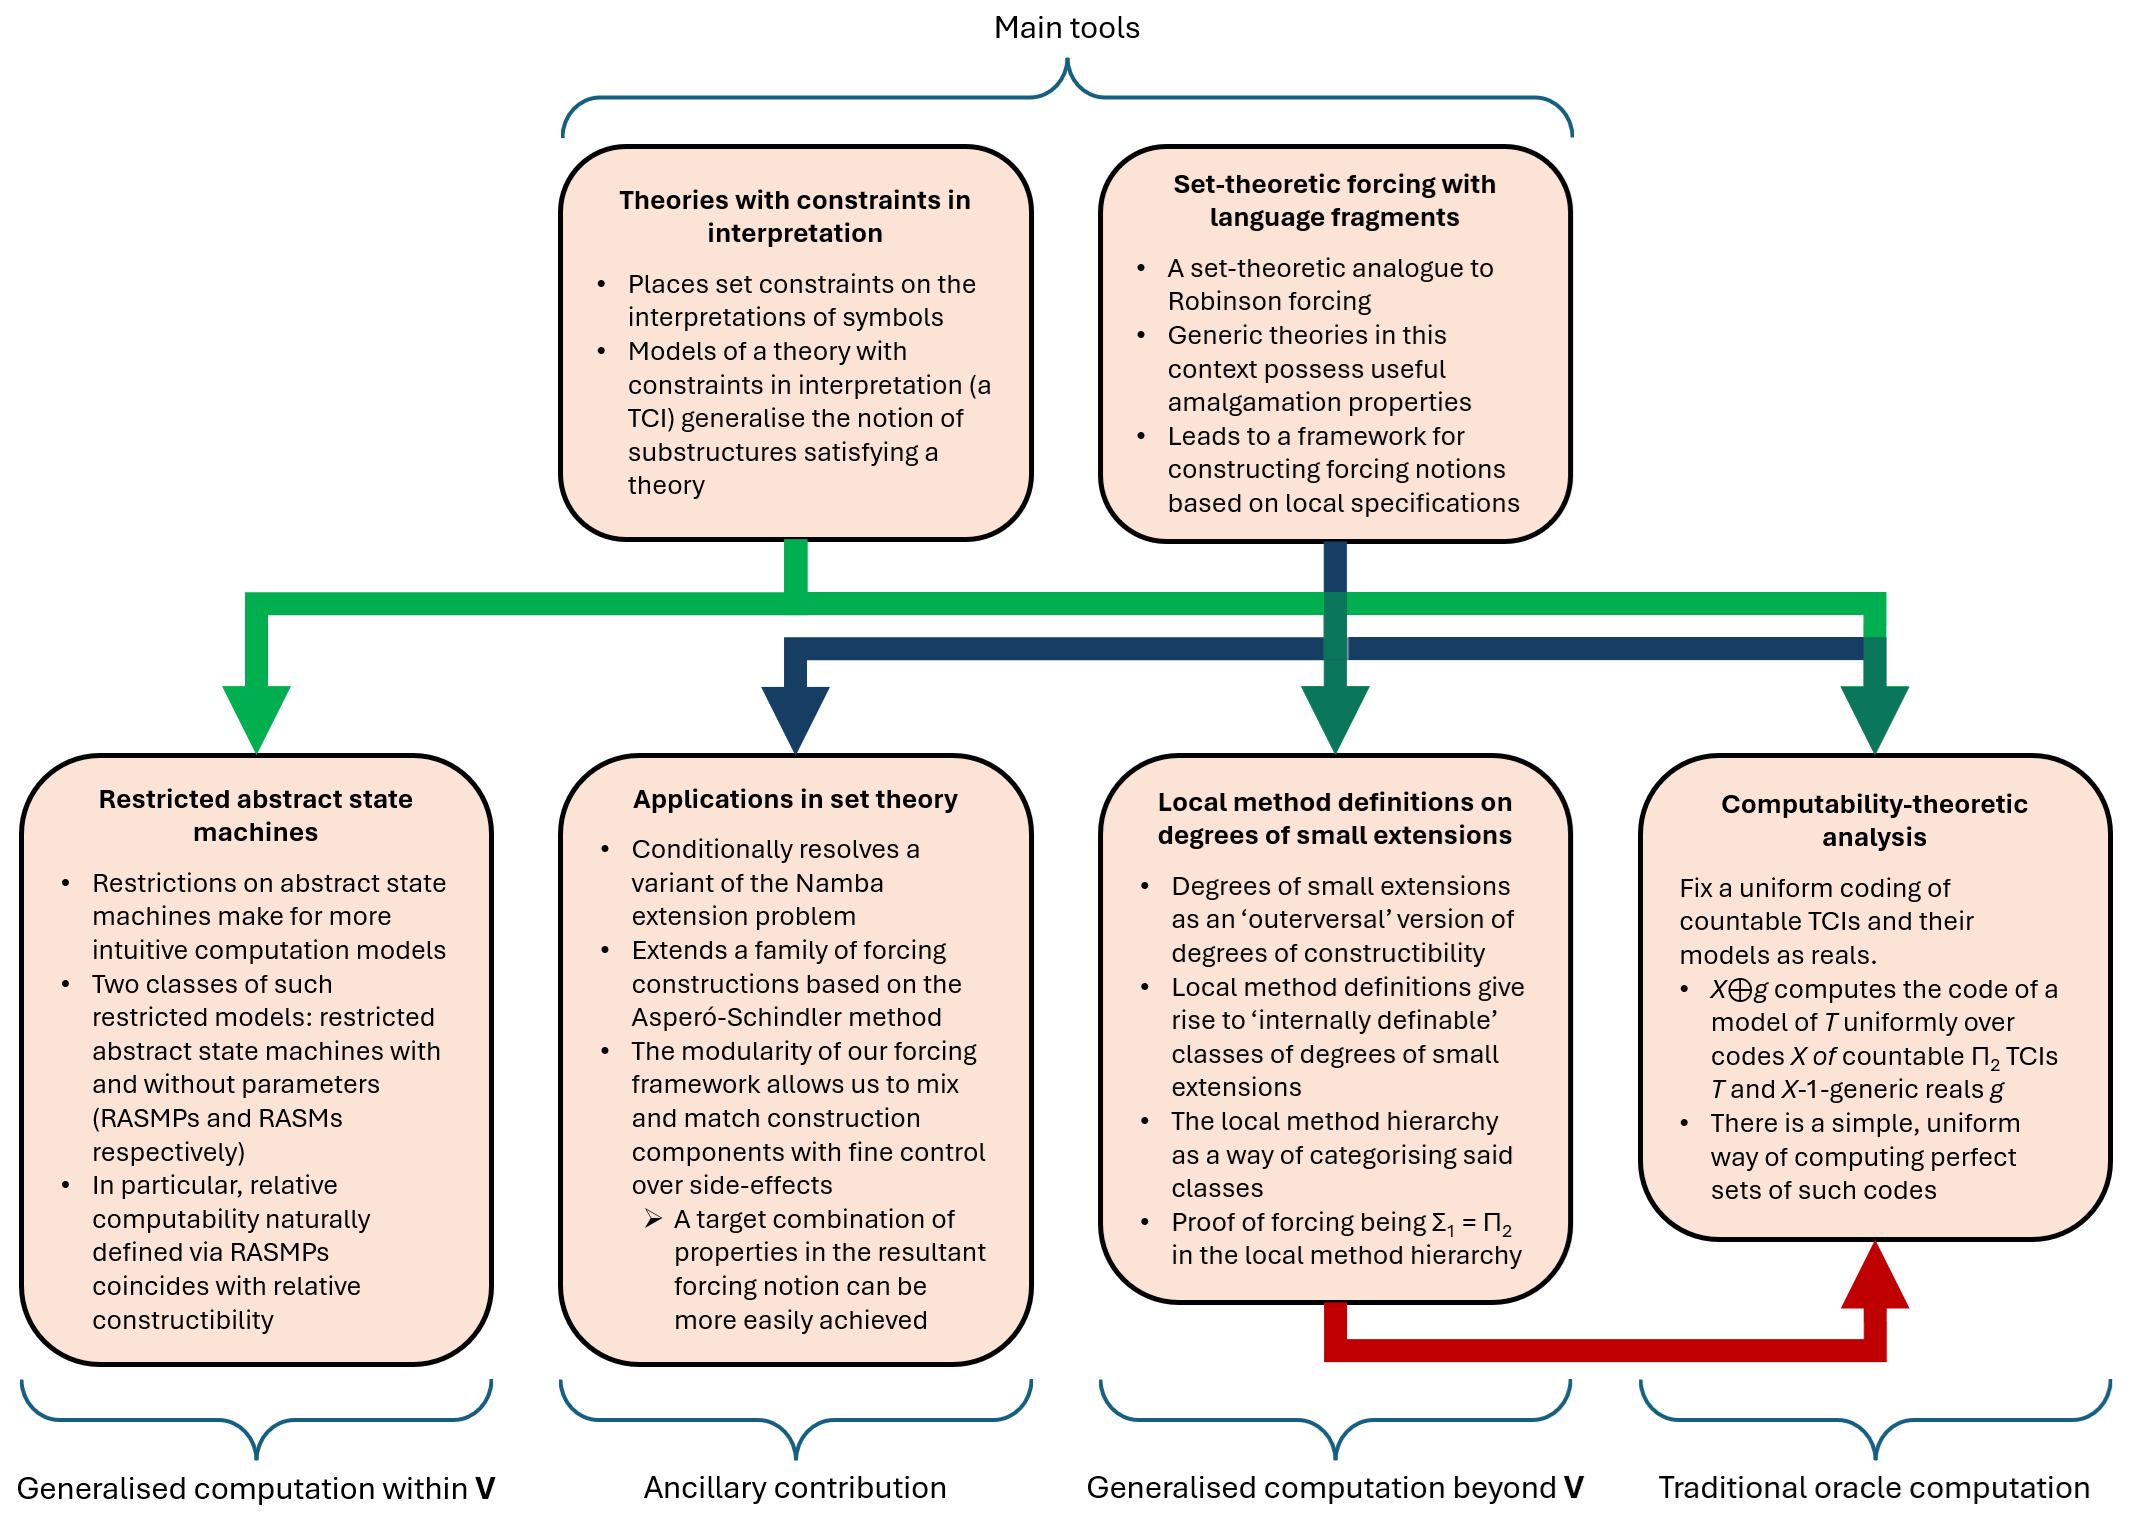
\includegraphics[width=\textwidth]{Overview_Chart.png}}
    \captionsetup{width=0.9\textwidth, format=hang}
    \caption[Key components of thesis]{An overview of this thesis in the form of a flowchart --- or to be more precise --- a summary of the key components of the author's contributions, together with the relations among them.}
    \label{overview}
\end{sidewaysfigure}

\clearpage

\blankpage

\mainmatter

\part{Background and Preamble}

\chapter{Introduction}\label{sect1}

A significant impetus for formalisations of computation in the early 20th century stemmed from Hilbert's programme, a programme which aimed ``to justify classical systems, in particular arithmetic, in terms of notions as intuitively clear as possible'' \cite{godelcw2}. In what might be aptly termed a fruitful detour, the models of computation thus formalised became the basis for a distinct but no less deep area of research: theoretical computer science. The vast majority of computer scientists now agree that the power of finitary computation is exactly captured by any (all) of the esteemed models conceived some 90 years ago. This consensus is the famous Church-Turing thesis.

In 1958, past Kleene's coining of the ``Church-Turing thesis'' in \cite{kleene}, G\"{o}del argued that Hilbert's original search space for his ``intuitively clear'' notions --- ``the domain of `finitary mathematics''' --- was unnaturally restrictive, for ``one has to admit at least some abstract notions in a consistency proof; the necessity of this is shown both by the second incompleteness theorem and by our experience with known consistency proofs, all of which appeal at some point to an abstract notion'' \cite{godelcw2}. Here, the word ``abstract'' was used to mean ``far from finitary/finitistic'', according to Troelstra. In the same work, G\"{o}del informally described a notion of potentially infinitary computation built inductively from natural numbers. As a class of objects, he called this notion \textit{computable functions of finite type}, wherein ``a computable function of type $(\sigma)\tau$ is a well-defined mathematical prodecure which, when applied to a computable function of type $\sigma$, yields a computable function of type $\tau$. Here a `well-defined mathematical procedure' must be taken as an understood primitive notion''. Hence, some level of tolerance is implied for such procedures to possess infinitary content, insofar as they are intuitively ``atomic'' for their purposes and within their contexts. It seems then that, like models of finitary computation, models of infinitary computation can too find their roots in Hilbert's programme.

If G\"{o}del's conception of infinitary computation in 1958 were informal and implicit, do explicit and formal conceptions exist? The answer is an emphatic ``\textit{Yes.}'' In fact, such models of infinitary computation are not new. Well-known exemplars go back as far as the 1980s, in the form of Blum-Shub-Smale (BSS) machines \cite{bss}. BSS machines were born from the study of dynamical systems, as their inventors investigated how iterated applications of simple functions on real numbers can give rise to unexpected complexity. About a decade later, Hamkins and Lewis unveiled a class of infinitary extensions of classical Turing machines, which they termed infinite time Turing machines, or ITTMs \cite{ittm}. Unlike BSS machines, ITTMs were intended more as a philosophical exploration in and of itself than a mathematical tool, even though they provide machine models corresponding to some complexity classes in (effective) descriptive set theory. Note that both BSS machines and ITTMs are computation models with reals as their intended input and output. More recent conceptions of a similar flavour include the MS-machines by Yang (see e.g. \cite{yangyue}).

Even older are implicit but formal models of infinitary computation. Many can be traced back to the 1960s, when Takeuti \cite{takeuti}, Kreisel and Sacks \cite{kreiselsacks} and others independently came up with notions of computability and relative computability on arbitrary sets of ordinals. Due to their ample similarities, the ideas associated with these notions eventually coalesced into a field now known as $\alpha$-recursion theory. Another formalisation of computability on infinite classes, formulated in the 1970s by Normann \cite{normann}, went on to become the central subject of study in $E$-recursion theory. The aforementioned notions only implicitly model infinitary computation because they define what it means to be (relatively) computable without explicitly defining what a computation entails. However, since computable classes in both paradigms are exactly those definable by certain types of formulas over a model of set theory, one can argue that it is justifiable to view formulas in general as an analogue of programs. 

Notably, the ``formulas as programs'' viewpoint already arises in classical computability theory, when one is introduced to the (relativised) arithmetical hierarchy. Oft-repeated in this context is the idea that oracle machines, from a functional perspective, are just sufficiently simple parametrised formulas in the language of arithmetic. As an implication, classical computation is but a kind of first-order definition (in the model-theoretic sense), which in turn, is precisely how most sets are generated. Following this line of thought, $\alpha$-recursion theory and $E$-recursion theory appear to be rather natural studies of how classical computation might generalise to the infinite. This prompts the following question.
\begin{align}\label{motqn}
\begin{split}
    & \textit{What happens if we take the common thread that is ``definable set} \\ 
    & \textit{generation as computation'' to its logical extreme?}
\end{split}
\end{align}
As the reader will discover in the subsequent chapters, (\ref{motqn}) is the motivating question of this thesis.

It is important to note that (\ref{motqn}) is neither a frivolous question nor a purely philosophical musing. In the field of set theory, where all kinds of large infinite objects are regularly dealt with, ``definable set generation as computation'' is a creed sometimes invoked without elaboration, as if it is self-evident. When we examine the inductive, hierarchical construction of the constructible universe $L$, it is easy to see that every set can be defined by a formula of some specific form, parametrised by ordinals. Such a formula is sometimes called a \textit{code} of the particular set it defines (as in, say, \cite{koepke1}). The word ``code'' is used here as a synonym for ``recipe'', and indeed ``program'', through which a mathematical object can be computed. Another salient example of using ``code'' in this manner can be found in the definition of \textit{Borel codes} in descriptive set theory. If the association of ``code'' with computation seemed tenuous, more obvious and extreme invocations of ``definable set generation as computation'' can be exhibited. For example, a set theorist's answer to a question on MathOverflow draws parallels between a very involved inner model construction (of far higher complexity than the construction of $L$) and an algorithm \cite{grigor}.

Should the reader remain unconvinced of our premise of ``definable set generation as computation'', we present a higher analogue of the Church-Turing thesis in Section \ref{chap6}, where we identify three apparently unrelated models of generalised computation (\ref{gct1} to \ref{gct3}) as equivalent. Actually, that \ref{gct1} and \ref{gct3} are equivalent (Theorem \ref{thm275} and Corollary \ref{cor8343}) is implied by the results in \cite{koepke1}. Our original contribution is the independent formulation of a witness for \ref{gct2} within the same section. To add weight to our argument, we formalise a version of abstract algorithms while abiding by principles that are deemed necessary in models of classical computation. These principles, namely
\begin{itemize}
    \item \textit{boundedness}: ``there is a fixed finite bound on the number of configurations a computor can immediately recognise'', and
    \item \textit{locality}: ``a computor can change only immediately recognisable (sub)configurations'',
\end{itemize}
are isolated by Sieg in \cite{sieg} based on the beliefs espoused by Turing in the latter's works.

\section{Chapteral Content and Dependencies}

For a rough dependency chart of the chapters following this one, see Figure \ref{chapteral}. In the next few paragraphs, slightly more details are given.

Chapters \ref{sect15} to \ref{chap4} lay the technical foundation for the rest of the thesis. Potential philosophical and meta-theoretic concerns are addressed, prerequisite knowledge highlighted, and background readings recommended. Important definitions and conventions are made explicit, especially those that are more niched, and those that lack community consensus. Consequentially, the topics related to forcing and generic iterations --- found in Chapters \ref{subs24} and \ref{chap4} --- are given more careful and comprehensive treatments than the others. All chapters subsequent to Chapters \ref{sect15} and \ref{subs24} depend on them, whereas the material in Chapter \ref{chap4} is only referenced in Section \ref{ss43}.

Chapter \ref{setupsec} concerns itself with the development of our central framework for forcing. The technical machinery of this chapter is concentrated on Theorem \ref{uni}, which itself is a generalisation of Lemma \ref{main2}. On the other hand, Lemma \ref{main2} is the accessible and more applicable backbone of much of this thesis, a throughline tying all following chapters, short of Chapter \ref{chap6}, together. Other than Chapter \ref{chap6}, Section \ref{subs51} is notable for not depending on Lemma \ref{main2}, nor in fact, on any of Chapter \ref{setupsec}'s technology.

Chapter \ref{TCIsec} introduces the notions of (first-order) TCIs and models of TCIs, before relating them to forcing and genericity. In particular, Section \ref{subs51} develops the basic theory of TCIs and their models, and can be read right after Chapter \ref{sect15}. The other sections depend in part on the results of Chapter \ref{setupsec}, and give applications of Chapter \ref{setupsec}'s forcing framework to more general contexts of genericity. Here, genericity is investigated in both set-theoretic and computability-theoretic senses of the word. Even though Chapters \ref{chap6} and \ref{chap7} both depend on this chapter, Chapter \ref{chap6} only requires the material in Section \ref{subs51}.

The entirety of Chapter \ref{sect2} is devoted to applying the forcing framework developed in Chapter \ref{setupsec} to variants of the Namba extension problem. Said framework is used to construct specific forcing notions that give rise to generic extensions satisfying various sets of requirements. We start with a relatively simple construction in Theorem \ref{notion1}, before extending it to solve a more difficult problem in Theorem \ref{notion2}. No other chapter is dependent on what transpires here. (N.B. The proof of Lemma \ref{lem339} references Remark \ref{rempp} in parentheses, but there is no strict dependency --- the low level subtleties in the remark are unnecessary and might detract from the clarity of the proof.)

Chapters \ref{chap6} and \ref{chap7} are both primary payoffs of the tools we build in Part \ref{part2}, as well as the end product of our programme on generalised computation that is pretty much entirely the subject of this thesis. They are also terminal nodes in the chapteral dependency chart, in the sense that no chapters depend on either of them.

In Chapter \ref{chap6}, we adapt Gurevich's sequential algorithms for the purpose of infinitary computation, to obtain two classes of generalised algorithms. From each class, a relative computability relation on sets is derived. These relative computability relations can be viewed as analogues of the Turing reducibility relation on reals. One such relation is then shown to be equivalent to the relative constructibility relation in set theory. This chapter only assumes the reader is familiar with the basic properties of TCIs, and thus can be read right after Section \ref{subs51}.

In Chapter \ref{chap7}, we define a relative computability relation with the set-theoretic universe $V$ as a basis, before investigating what it means to access subclasses of degrees of this relation from within $V$ itself. We next introduce a paradigm to compare different methods of such access, one of which is (set) forcing. As it turns out, within this paradigm, forcing is exactly $\Sigma_1$ which in turn is exactly $\Pi_2$. It would not be a stretch to say that this chapter is the culmination of the main results of Part \ref{part2}, and is therefore highly dependent on Chapters \ref{setupsec} and \ref{TCIsec}.

\begin{figure}[!ht]
    \centering
    \centerline{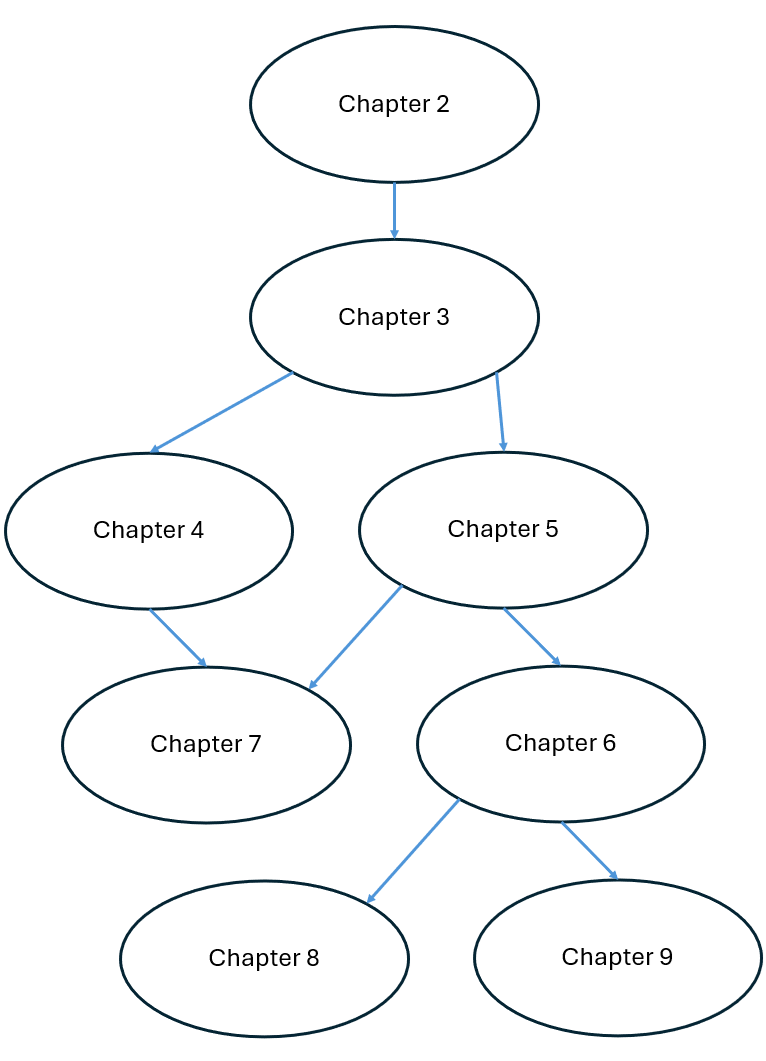
\includegraphics[width=0.95\textwidth]{Chapteral_Dependencies.png}}
    \captionsetup{width=\textwidth, format=hang}
    \caption[Dependencies among chapters]{A bare-bones chart of dependencies among Chapters 2 to 9.}
    \label{chapteral}
\end{figure}

\chapter{Preliminaries}\label{sect15}

\section{The Meta-theory}\label{subs21}

At the meta-level, it suffices to assume $\mathsf{ZFC}$. We frame relative consistency proofs involving additional assumptions as proofs of statements of the form $$\text{``}\mathrm{Con}(\mathsf{ZFC} + \phi) \implies \mathrm{Con}(\mathsf{ZFC} + \psi)\text{''}$$ over $\mathsf{ZFC}$, where $\phi$ is the conjunction of the relevant assumptions. Implicit are the invocations of G\"{o}del's completeness theorem at the meta-level, whenever we argue using models (a.k.a. \emph{universes}) of set theory.

Our meta-theoretic approach to forcing is only slightly more complicated. Conventionally we start with a countable transitive model of $\mathsf{ZFC}$, called a \emph{ground model}, which is not guaranteed to exist by our meta-theory. There are many ways to sidestep this problem and treat the statement ``countable transitive ground model'' as a convenient abuse of notation, a few of which are noted by Kunen in IV.5 of \cite{kunen}. We adopt the first approach detailed in IV.5.1 of \cite{kunen}, an approach that is pretty much standard in the community, and one we feel is most immediately and formally accessible.

\section{Basic Mathematical Logic}

Unless specified otherwise, we follow the standard definitions of concepts related to the syntax and semantics of first-order logic, as seen in e.g. \cite{enderton}.

\begin{con}\label{firstconv}
\leavevmode
\begin{enumerate}[label=(\arabic*)]
    \item We call any set of first order formulas a \emph{first-order language}.
    \item We assume the first-order languages we consider to contain only $\neg, \wedge, \vee, \implies, \iff$ as their zeroth-order logical symbols, interpreted semantically in the usual sense. 
    \item Each first-order logical symbol is identified with a unique member of $H(\omega) \setminus \omega$.
    \item Given a first-order language $\mathcal{L}$, let $\mathrm{Ter}(\mathcal{L})$ denote the set of all terms occurring in (some formula in) $\mathcal{L}$.
    \item The signature (in the abstract) can contain only relation symbols of a non-zero finite arity, function symbols of a non-zero finite arity, and constant symbols, identified as follows:
    \begin{itemize}
        \item a $n$-ary relation symbol is a triple of the form $(X, 0, n)$,
        \item a $n$-ary function symbol is a triple of the form $(X, 1, n)$, and
        \item a constant symbol is a pair of the form $(X, 2)$.
    \end{itemize}
    We call any such symbol a \emph{signature-related symbol}.
    \item A \emph{form-preserving signature embedding} is an injective function from a set of signature-related symbols into the class of signature-related symbols, such that
    \begin{itemize}
        \item $n$-ary relation symbols are mapped to $n$-ary relation symbols,
        \item $n$-ary function symbols are mapped to $n$-ary function symbols, and
        \item constant symbols are mapped to constant symbols.
    \end{itemize}
    \item\label{227} We will assume that the class of signature-related symbols is disjoint from the set of first-order logical symbols.
    \item An interpretation of a signature $\sigma$ is a function that maps
    \begin{itemize}
        \item each $n$-ary relation symbol in $\sigma$ to an $n$-ary relation,
        \item each $n$-ary function symbol in $\sigma$ to an $n$-ary function, and
        \item each constant symbol in $\sigma$ to a set.
    \end{itemize}
    Here, 
    \begin{itemize}
        \item an $n$-ary relation is formally a function from $A^n$ into $2$, for some set $A$, and
        \item an $n$-ary function is formally a function from $A^n$ into $A^n$, for some set $A$.
    \end{itemize}
    \item A first-order structure $\mathfrak{A}$ is presented in the form $(A; \mathcal{I})$, where $A$ is the base set of $\mathfrak{A}$ and $\mathcal{I}$ is an interpretation of some signature $\sigma$, such that whenever $\dot{X} \in \sigma$, $\mathcal{I}(\dot{X})$ --- which denotes \emph{the interpretation of} $\dot{X}$ \emph{in} $\mathfrak{A}$ --- fulfils the following.
    \begin{enumerate}[label=(\alph*)]
        \item If $\dot{X}$ is an $n$-ary relation or function symbol, then $dom(\mathcal{I}(\dot{X})) = A^n$.
        \item If $\dot{X}$ is a constant symbol, then $\mathcal{I}(\dot{X}) \in A$.
    \end{enumerate}
    In this presentation, the signature of $\mathfrak{A}$ --- denoted as $\sigma(\mathfrak{A})$ --- is simply $dom(\mathcal{I})$. Furthermore, we shall \begin{itemize}
        \item refer to $\mathcal{I}$ as $\mathcal{I}^{\mathfrak{A}}$ when there is no need to mention $A$, and
        \item refer to $\mathcal{I}(\dot{X})$ as $\dot{X}^{\mathfrak{A}}$ when there is no need to mention $\mathcal{I}$.
    \end{itemize} 
    
    In contexts where the correspondence between a signature and its interpretation is clear, we might write $(A; \mathcal{I})$ as $(A; \Vec{S})$, where $\Vec{S}$ is some ordering of $ran(\mathcal{I})$.
    \item\label{224} The variables occurring in any first-order formula must come from a fixed countably infinite set $\mathrm{Var}$. We will assume that $\mathrm{Var}$ is disjoint from both the set of first-order logical symbols and the class of signature-related symbols.
    \item A string over a vocabulary set $\Sigma$ is a member of $\Sigma^{< \omega}$.
    \item We sometimes define procedures in which subformulas of a first-order formula are replaced by other formulas. In these cases, for convenience's sake, what follows will be adopted.
    \begin{quote}
        Let 
        \begin{itemize}
            \item $\phi$ be a first-order formula, 
            \item $\varphi$ be a subformula of $\phi$, and
            \item $\ulcorner x \urcorner$ be a variable occurring in $\phi$.
        \end{itemize}
        Suppose we are to replace $\varphi$ in $\phi$ with some formula $\varphi'$. Let $\ulcorner y \urcorner$ be a bound variable in $\varphi'$. Unless otherwise stated, we always assume $$\ulcorner x \urcorner \neq \ulcorner y \urcorner \text{.}$$        
    \end{quote}
\end{enumerate}
\end{con}

We write ``structure(s)'' as the abbreviation of ``first-order structure(s)'' henceforth. There should be no confusion as these are the only type of structures we will be dealing with.

\begin{defi}
Given any set $X$ and any signature $\sigma$, the \emph{language associated with} $(X; \sigma)$ is the set of first-order formulas over $\sigma$ with parameters from $X$. Similarly, given any structure $\mathfrak{A} = (A; \mathcal{I})$, the \emph{language associated with} $\mathfrak{A}$ is the set of first-order formulas over the signature of $\mathfrak{A}$ with parameters from $A$.
\end{defi}

\begin{defi}
For any structure $\mathfrak{A} = (A; \mathcal{I})$, a $\mathfrak{A}$\emph{-valuation} is a function from $\mathrm{Var}$ into $A$.
\end{defi}

\begin{defi}
The \emph{size of a structure} $\mathfrak{A} = (A; \mathcal{I})$ is equal to $$max\{|A|, |\mathcal{I}|\}.$$ We say $\mathfrak{A}$ is a \emph{countable structure} iff its size is a countable cardinal.
\end{defi}

\begin{defi}\label{def25}
Let $\phi$ be a first-order formula over a signature $\sigma$. We inductively define what it means for $\phi$ to be $\Pi_n$ or $\Sigma_n$ as $n$ ranges over the natural numbers.
\begin{enumerate}[label=(\arabic*)]
    \item If $n = 0$, then $\phi$ is $\Pi_0$ iff $\phi$ is $\Sigma_0$ iff $\phi$ is quantifier-free.
    \item\label{3292} If $n = m + 1$ for some $m < \omega$, then 
    \begin{enumerate}[label=(\alph*)]
        \item\label{3292a} $\phi$ is $\Pi_n$ iff there is a $\Sigma_m$ formula $\varphi$, a number $k < \omega$, and variable symbols $x_1, \dots, x_k$ not bound in $\varphi$, such that 
        \begin{equation*}
            \phi = \ulcorner \forall x_1 \dots \forall x_k \ \varphi \urcorner \text{, and}
        \end{equation*}
        \item\label{3292b} $\phi$ is $\Sigma_n$ iff there is a $\Pi_m$ formula $\varphi$, a number $k < \omega$, and variable symbols $x_1, \dots, x_k$ not bound in $\varphi$, such that 
        \begin{equation*}
            \phi = \ulcorner \exists x_1 \dots \exists x_k \ \varphi \urcorner \text{.}
        \end{equation*}
    \end{enumerate}
\end{enumerate}
Note that if $k = 0$ in \ref{3292}\ref{3292a} and \ref{3292}\ref{3292b}, then $\phi$ is $\Sigma_m$ and $\Pi_m$ respectively.
\end{defi}

\begin{defi}
Let $X$ and $Y$ be finite tuples. Then $X^\frown Y$ denotes the concatenation of $X$ with $Y$. More formally, 
\begin{equation*}
    X^\frown Y := X \cup \{(|X|+i, y) : (i, y) \in Y\} \text{.}
\end{equation*}
Notice that the operation $^\frown$ is associative on finite tuples.
\end{defi}

\section{Basic Set Theory}

Unless specified otherwise, we follow the standard definitions of concepts typically encountered in a foundational set theory course, following e.g. \cite{jechhrbacek}.

\begin{con}
\leavevmode
\begin{enumerate}[label=(\arabic*)]
    \item Unless otherwise specified, $V$ always refers to the universe we are currently working in. For all practical purposes, we can assume it is a countable transitive model of $\mathsf{ZFC}$, so that it doubles as a ground model in case forcing arguments are to be run.
    \item We adopt the set-theoretic interpretation of functions as sets of ordered pairs satisfying certain properties. So when we say a function is definable, we actually mean its graph is definable as a set --- usually a subset of an ambient structure that should be clear in context, if not explicitly mentioned.
    \item We fix in $V$, a distinguished first-order relation symbol $\ulcorner \in \urcorner$.
    \item A first-order formula is \emph{in the language of set theory} iff it is a formula over the signature $\{\ulcorner \in \urcorner\}$.
    \item\label{stcon1} We say a structure $\mathfrak{A}$ is \emph{a structure in the language of set theory} iff 
    \begin{itemize}
        \item the signature of $\mathfrak{A}$ is the singleton set $\{\ulcorner \in \urcorner\}$, and
        \item $\mathfrak{A}$ interprets $\ulcorner \in \urcorner$ as the membership relation on $V$ restricted to the base set of $\mathfrak{A}$.
    \end{itemize}
    More formally, $$\mathfrak{A} = (A; \mathcal{I}) \text{ and } \mathcal{I} = \{(\ulcorner \in \urcorner, \in \cap \ A)\},$$ where $\in$ is the membership relation on $V$. In this case, we can just write $\mathfrak{A} = (A; \in)$.
    \item A first-order formula is \emph{in a possibly expanded language of set theory} iff it is a formula over some signature $\sigma$ satisfying $\ulcorner \in \urcorner \in \sigma$.
    \item We say a structure $\mathfrak{A}$ is \emph{a structure in a possibly expanded language of set theory} iff we omit the cardinality requirement on the signature of $\mathfrak{A}$ in \ref{stcon1}. More formally, $$\mathfrak{A} = (A; \mathcal{I}) \text{ and } \mathcal{I} = \{(\ulcorner \in \urcorner, \in \cap \ A)\} \cup \Vec{X},$$ where $\Vec{X}$ is some function and $\in$ is the membership relation on $V$. In this case, we can just write $\mathfrak{A} = (A; \in, \Vec{X})$.
    \item\label{idu} We identify a universe of set theory $W$ with the structure $(W; \in)$. This should not cause confusion in the circumstances we find ourselves in.
    \item When $\alpha$ and $\beta$ are ordinals, we write ``$\alpha < \beta$'' to mean ``$\alpha \in \beta$''.
    \item A natural number is a member of the ordinal $\omega$. In other words, we view $\omega$ as the set of all natural numbers.
    \item A real is a subset of $\omega$. We identify a real with its characteristic function on $\omega$, as is standard in computability theory. As in \ref{idu}, this ambiguity should not cause any confusion.
\end{enumerate}
\end{con}

We overload and expand on Definition \ref{def25} when dealing with the special case of set-theoretic languages. 

\begin{defi}[L\'{e}vy hierarchy]\label{def27}
Let $\phi$ be a first-order formula over a possibly expanded language of set theory. We inductively define what it means for $\phi$ to be $\Delta_n$, $\Pi_n$ or $\Sigma_n$ as $n$ ranges over the natural numbers.
\begin{enumerate}[label=(\arabic*)]
    \item\label{def271} If $n = 0$, then $\phi$ is $\Delta_n$ iff $\phi$ is $\Pi_n$ iff $\phi$ is $\Sigma_n$ iff every quantifier occurring in $\phi$ is bounded by $\in$.
    \item\label{2712} If $n = m + 1$ for some $m < \omega$, then 
    \begin{enumerate}[label=(\alph*)]
        \item\label{2712a} $\phi$ is $\Pi_n$ iff there is a $\Sigma_m$ formula $\varphi$, a number $k < \omega$, and variable symbols $x_1, \dots, x_k$ not bound in $\varphi$, such that 
        \begin{equation*}
            \phi = \ulcorner \forall x_1 \dots \forall x_k \ \varphi \urcorner \text{,}
        \end{equation*}
        \item\label{2712b} $\phi$ is $\Sigma_n$ iff there is a $\Pi_m$ formula $\varphi$, a number $k < \omega$, and variable symbols $x_1, \dots, x_k$ not bound in $\varphi$, such that 
        \begin{equation*}
            \phi = \ulcorner \exists x_1 \dots \exists x_k \ \varphi \urcorner \text{, and}
        \end{equation*}
        \item $\phi$ is $\Delta_n$ iff 
        \begin{itemize}[label=$\circ$]
            \item $\phi$ is $\Pi_n$, and
            \item for some $\Sigma_n$ formula $\varphi$,
            \begin{equation*}
                \mathsf{ZFC} \vdash \phi \iff \varphi \text{.}
            \end{equation*}
        \end{itemize}
    \end{enumerate}
\end{enumerate}
Note that if $k = 0$ respectively in \ref{2712}\ref{2712a} and \ref{2712}\ref{2712b}, then $\phi$ is $\Sigma_m$ and $\Pi_m$ respectively.
\end{defi}

Most of the time, the context should indicate clearly which interpretation to adopt. Nevertheless, we shall try as much as possible to disambiguate things in this respect, and highlight each time Definition \ref{def27} is used instead of Definition \ref{def25}.

\begin{defi}
Let $X$ be a set and $\mathfrak{A}$ be a structure in a possibly expanded language of set theory with base set $A$. We say $X$ is \emph{definable in the language associated with} $\mathfrak{A}$ iff $$X = \{y \in A : \mathfrak{A} \models \phi(y)\}$$ for some formula $\phi$ with one free variable in the language associated with $\mathfrak{A}$.
\end{defi}

\begin{defi}\label{def29}
Let 
\begin{itemize}
    \item $X$ be a set,
    \item $\mathfrak{A}$ be a structure in a possibly expanded language of set theory with base set $A$, and
    \item $n < \omega$. 
\end{itemize} 
We say $X$ is $\Sigma_n$\emph{-definable} (resp. $\Pi_n$\emph{-definable} and $\Delta_n$\emph{-definable}) \emph{in the language associated with} $\mathfrak{A}$ iff $$X = \{y \in A : \mathfrak{A} \models \phi(y)\}$$ for some $\Sigma_n$ (resp. $\Pi_n$ and $\Delta_n$) formula (in accordance with Definition \ref{def27}) $\phi$ with one free variable in the language associated with $\mathfrak{A}$.
\end{defi}

We can generalise Definition \ref{def29} by relaxing the language requirement.

\begin{defi}
Let 
\begin{itemize}
    \item $X$ be a class, 
    \item $\mathfrak{A}$ be a structure in a possibly expanded language of set theory with base class $A$ and signature $\sigma$, such that 
    \begin{itemize}[label=$\circ$]
        \item $A$ is transitive, and
        \item $\mathfrak{A} \models \mathsf{ZFC}$, and
    \end{itemize}
    \item $n < \omega$.
\end{itemize}
We say $X$ is $\Sigma_n$\emph{-definable} (resp. $\Pi_n$\emph{-definable} and $\Delta_n$\emph{-definable}) \emph{in} $\mathfrak{A}$ iff $$X = \{y \in A : \mathfrak{A} \models \phi(y)\}$$ for some $\Sigma_n$ (resp. $\Pi_n$ and $\Delta_n$) formula (in the sense of Definition \ref{def27}) $\phi$ with one free variable over $\sigma$.

If in addition,
\begin{itemize}
    \item $\mathfrak{A} = (A; \in)$, and
    \item $\sigma = \{\ulcorner \in \urcorner\}$,
\end{itemize}
we may identify $\mathfrak{A}$ with $A$ and say $X$ is $\Sigma_n$\emph{-definable} (resp. $\Pi_n$\emph{-definable} and $\Delta_n$\emph{-definable}) \emph{in} $A$ iff $X$ is $\Sigma_n$-definable (resp. $\Pi_n$-definable and $\Delta_n$-definable) in $\mathfrak{A}$. 

We say $X$ is $\Sigma_n$\emph{-definable} (resp. $\Pi_n$\emph{-definable} and $\Delta_n$\emph{-definable}) iff $X$ is $\Sigma_n$-definable (resp. $\Pi_n$-definable and $\Delta_n$-definable) in $\mathfrak{A}'$ for every structure $\mathfrak{A}'$ in a possibly expanded language of set theory such that
\begin{enumerate}[label=(\alph*)]
    \item $\mathfrak{A}'$ has a transitive base class, and
    \item $\mathfrak{A}' \models \mathsf{ZFC}$.
\end{enumerate}
\end{defi}

\begin{defi}
Let $A$ and $X$ be classes. We say $X \in \mathbf{\Sigma_n}(A)$ (resp. $X \in \mathbf{\Pi_n}(A)$ and $X \in \mathbf{\Delta_n}(A)$) iff
\begin{enumerate}[label=(\alph*)]
    \item $X$ is $\Sigma_n$-definable (resp. $\Pi_n$-definable and $\Delta_n$-definable) in $A$, and
    \item $X \subset ORD$.
\end{enumerate}
\end{defi}

\begin{defi}
Let $\mathfrak{A}$ be a structure in a possibly expanded language of set theory. When we say 
\begin{equation}\label{eq11}
    \text{``}\mathfrak{A} \textit{ is a model of a sufficiently strong set theory'',} 
\end{equation}
we mean to emphasise the low strength of the set theory $\mathfrak{A}$ satisfies. 

In more concrete terms, what we typically term a \emph{set theory}, is a set of first-order formulas in the language of set theory. Examples of set theories include
\begin{enumerate}[label=(\roman*)]
    \item the set of axioms of $\mathsf{ZFC}$, and
    \item the set of axioms of \textit{Kripke-Platek set theory} (\emph{without infinity}), denoted $\mathsf{KP}$, which is a much weaker theory than $\mathsf{ZFC}$.
\end{enumerate} 
For convenience's sake, one may always assume (\ref{eq11}) to mean 
\begin{quote}
    $\text{``}\mathfrak{A} \models T \text{ for some set theory } T \text{ such that}$ 
    \begin{itemize}
        \item $\mathsf{KP} \subset T$, and
        \item $T \vdash \ulcorner \forall x \ (\text{``} x \text{ is Dedekind-finite} \implies x \text{ is finite''}) \urcorner$''.
    \end{itemize}
\end{quote}
\end{defi}

\begin{defi}
Given (externally) a class $\mathbf{M}$ of classes, we say a definition $\varphi$ in $n$ variables --- for some finite number $n$ --- is \emph{absolute for} $\mathbf{M}$ iff for every two members $X, Y$ of $\mathbf{M}$ such that $X \subset Y$, and for every sequence $\Vec{x}$ of $n$ members of $X$,
\begin{equation*}
    X \models \varphi(\Vec{x}) \iff Y \models \varphi(\Vec{x}) \text{.}
\end{equation*}
\end{defi}

\begin{defi}\label{inoutmodels}
We say $V'$ is a \emph{weak inner model} of $W$ (or equivalently, $W$ is a \emph{weak outer model} of $V'$) iff
\begin{enumerate}[label=(\alph*)]
    \item $V'$ and $W$ are both models of $\mathsf{ZFC}$,
    \item $V' \subset W$, and
    \item $V'$ is a \textit{transitive class in} $W$, that is, $x \cap W \subset V'$ for each $x \in V'$.
\end{enumerate}
If in addition, $V'$ and $W$ share the same ordinals i.e. $ORD^{V'} = ORD^W$, then $V'$ is an \emph{inner model} of $W$ (or equivalently, $W$ is an \emph{outer model} of $V'$).
\end{defi}
\begin{defi}
Let $Y$ be any set.

We say $X$ \emph{codes} $Y$ (or equivalently, $X$ \emph{is a code of} $Y$) iff 
\begin{enumerate}[label=(\alph*)]
    \item $X$ is a set of ordinals, and
    \item every transitive model of $\mathsf{ZFC - Powerset}$ containing $X$ also contains $Y$.
\end{enumerate}

$X$ \emph{codes} $Y$ \emph{as a real} iff $X$ codes $Y$ and $X \subset \omega$.

$Y$ \emph{has a real code} (or equivalently, $Y$ \emph{can be coded as a real}) iff $X$ codes $Y$ as a real for some $X$.
\end{defi}

\begin{lem}\label{setcode}
Let $X$ be a set with $|trcl(X)| = \kappa$. Then there is $A \subset \kappa$ such that $A$ codes $X$.

In particular, any set with a countable transitive closure has a real code.
\end{lem}

\begin{proof}
Let $Y := trcl(X) \cup \{X\}$. Note that 
\begin{equation}\label{trcluni}
    X \text{ is the unique } \! \in \!\text{-maximal member of } Y
\end{equation} 
in any transitive model of $\mathsf{ZFC - Powerset}$ containing $Y$. Choose any bijection $f$ from $Y$ into $\kappa$. Define $$R := \{(f(x), f(y)) \in \kappa \times \kappa : x, y \in Y \text{ and } x \in y\}.$$ Now $R$ can be thought of as a subset $A$ of $\kappa$ via the canonical G\"{o}del numbering of pairs. If $V'$ is a transitive model of $\mathsf{ZFC - Powerset}$ containing $A$, then we can recover $R$ in $V'$ by computing the inverse of $A$ under G\"{o}del's pairing function. The Mostowski collapse function works on $R$ in $V'$ to give us $Y \in V'$. This implies $X \in V'$ since $X$ is definable from $Y$ according to (\ref{trcluni}). 
\end{proof}

Notice that the decoding process of $A$ to obtain $X$, as described in the proof of Lemma \ref{setcode}, is absolute for transitive models of $\mathsf{ZF}$, because all of its components are. 

\section{Basic Computability Theory}

Unless specified otherwise, we follow the standard definitions of concepts typically encountered in a foundational computability theory course, following e.g. \cite{soarebook}.

\begin{con}\label{comcon}
\leavevmode
\begin{enumerate}[label=(\arabic*)]
    \item\label{cc1} We call a Turing machine equipped with an oracle, an oracle machine. Vanilla Turing machines without oracles can be thought of as oracle machines of which state transition functions do not depend on oracle reads. Further, any oracle machine with trivial (e.g. empty) oracle input can be simulated by a vanilla Turing machine. So for convenience, and since we often require the use of oracles, we do not distinguish between Turing machines and oracle machines. In fact, from now on we will only mention oracle machines.
    \item\label{ctc} Oracle machines are always assumed to take as input, some natural number. More than that, we shall assume that every natural number is a valid input for every oracle machine. This is obviously an abstraction, but it is an easy one to realise. This is because every natural number can be uniquely represented by a finite binary string, and so by the usual definition of an oracle machine, any machine with alphabet size $2$ is a realisation.
    \item To follow up on \ref{ctc}, every binary string $\tau \in 2^{< \omega}$ represents a (unique) natural number, and we write $\langle \tau \rangle$ to mean the natural number $\tau$ represents.
    \item We will, whenever a suitable context arises, use the term ``oracle machine'' to mean ``Turing functional with oracle''. In other words, if an oracle machine halts on any input, it must return either $0$ or $1$. 
    \item There is a computable enumeration of (the finite codes of) all oracle machines, so that it is always possible to simulate the $e$-th oracle machine for $s$ steps, as long as $e$ and $s$ are natural numbers.
    \item We fix in advance, a computable enumeration of oracle machines, so that for any $e \in \omega$, $\Phi_e$ refers to the $e$-th oracle machine in this particular enumeration.
\end{enumerate}
\end{con}

\begin{defi}
If $\Phi$ is an oracle machine and $A \subset \omega$, we write $\Phi^A$ to mean the set
\begin{equation*}
    \{n \in \omega : \Phi \text{ with oracle input } A \text{ halts on input } n \text{ and returns } 1\} \text{.}
\end{equation*}
The appearance of $\Phi^A$ always implicitly implies $\Phi$ with oracle input $A$ halts on every natural number input.
\end{defi}

\begin{defi}
If $A \subset \omega$, $X \subset 2^{< \omega}$ and $\Phi$ is an oracle machine, we overload $\Phi^A$ so that also, $\Phi^A = X$ iff
\begin{equation*}
    \Phi^A = \{\langle \tau \rangle : \tau \in X\} \text{.}
\end{equation*}
\end{defi}

\begin{defi}
Let $A \subset \omega$. Then $A'$ denotes the \emph{relativised halting problem for} $A$, i.e. $$A' := \{e \in \omega : \Phi_e \text{ with oracle input } A \text{ halts on input } e\} \text{.}$$ 
\end{defi}

By \ref{cc1} of Convention \ref{comcon}, $\emptyset'$ is Turing-equivalent to typical definitions of the standard halting problem.

\begin{defi}
We call the signature $$\{+, \times, 0, 1, \leq\}$$ \emph{the language of arithmetic}. 
\end{defi}

\begin{defi}
By the \emph{standard natural number structure} $\mathbb{N}$, we mean the first-order structure with base set $\omega$ interpreting the language of arithmetic such that
\begin{enumerate}[label=(\alph*)]
    \item $+$ is interpreted to mean addition on the natural numbers,
    \item $\times$ is interpreted to mean multiplication on the natural numbers,
    \item $0$ and $1$ are interpreted to mean ordinals $0$ and $1$ respectively, and
    \item $\leq$ is interpreted to mean the total ordering of the natural numbers.
\end{enumerate} 
In other words, we really write $\mathbb{N}$ to mean the standard structure on the natural numbers over the language of arithmetic.
\end{defi}

\begin{defi}[Arithmetical hierarchy]
Let $\phi$ be a first-order formula over the language of arithmetic. We inductively define what it means for $\phi$ to be $\Delta^0_n$, $\Pi^0_n$ or $\Sigma^0_n$ as $n$ ranges over the natural numbers.
\begin{enumerate}[label=(\arabic*)]
    \item If $n = 0$, then $\phi$ is $\Delta^0_n$ iff $\phi$ is $\Pi^0_n$ iff $\phi$ is $\Sigma^0_n$ iff every quantifier occurring in $\phi$ is bounded by $\leq$.
    \item If $n = m + 1$ for some $m < \omega$, then 
    \begin{enumerate}[label=(\alph*)]
        \item $\phi$ is $\Pi^0_n$ iff there is a $\Sigma^0_m$ formula $\varphi$, a number $k < \omega$, and variable symbols $x_1, \dots, x_k$ not bound in $\varphi$, such that 
        \begin{equation*}
            \phi = \ulcorner \forall x_1 \dots \forall x_k \ \varphi \urcorner \text{,}
        \end{equation*}
        \item $\phi$ is $\Sigma^0_n$ iff there is a $\Pi^0_m$ formula $\varphi$, a number $k < \omega$, and variable symbols $x_1, \dots, x_k$ not bound in $\varphi$, such that 
        \begin{equation*}
            \phi = \ulcorner \exists x_1 \dots \exists x_k \ \varphi \urcorner \text{, and}
        \end{equation*}
        \item $\phi$ is $\Delta^0_n$ iff 
        \begin{itemize}[label=$\circ$]
            \item $\phi$ is $\Pi^0_n$, and
            \item for some $\Sigma^0_n$ formula $\varphi$,
            \begin{equation*}
                \mathsf{ZFC} \vdash \phi \iff \varphi \text{.}
            \end{equation*}
        \end{itemize}
    \end{enumerate}
\end{enumerate}
Note that if $k = 0$ respectively in \ref{2712}\ref{2712a} and \ref{2712}\ref{2712b}, then $\phi$ is $\Sigma^0_m$ and $\Pi^0_m$ respectively.
\end{defi}

\begin{defi}
For $X \subset 2^{< \omega}$, we say $X$ is a \emph{tree} iff $X$ is closed under predecessors with respect to the subset relation. More formally, $X$ is a tree iff whenever $\tau_1 \in X$ and $\tau_2 \in 2^{< \omega}$, 
\begin{equation*}
    \tau_2 \subset \tau_1 \implies \tau_2 \in X \text{.}
\end{equation*}
Often, we say $X$ \textit{is a subtree of} $2^{<\omega}$ when we mean $X \subset 2^{< \omega}$ and $X$ is a tree.
\end{defi}

\begin{defi}
If $X \subset 2^{< \omega}$ is a tree, then
\begin{equation*}
    [X] := \{x \in 2^{\omega} : x \text{ is a branch through } X\} \text{.}
\end{equation*}
\end{defi}

\begin{defi}
Let $X \subset 2^{< \omega}$ be a tree. Then $\tau$ is a splitting node in $X$ iff $\tau^\frown (0) \in X$ and $\tau^\frown (1) \in X$.
\end{defi}

\begin{defi}
A set $X \subset 2^{< \omega}$ is a \emph{perfect tree} iff $X$ is a tree, and for every $\tau_1 \in X$ there is $\tau_2$ such that $\tau_1 \subset \tau_2$ and $\tau_2$ is a splitting node in $X$.

A set $X \subset 2^{< \omega}$ is a \emph{uniformly splitting tree} iff $X$ is a tree, and for every splitting node $\tau_1$ in $X$ and every $\tau_2 \in X$, 
\begin{equation*}
    |\tau_1| = |\tau_2| \implies \tau_2 \text{ is a splitting node in } X \text{.}
\end{equation*}
\end{defi}

Notice that whenever $X$ is a perfect tree, $[X]$ is a perfect set in the Cantor space $2^{\omega}$.

\begin{defi}
Let $n < \omega$. A real $A \in 2^{\omega}$ is $n$\emph{-generic} iff for each $\Sigma^0_n$ formula $\phi$ over the language of arithmetic with a single free variable $x$, one of the following holds.
\begin{enumerate}[label=(\alph*)]
    \item For some $n < \omega$, $A \restriction n \in D_{\phi}$, where $$D_{\phi} := \{\tau \in 2^{< \omega} : \mathbb{N} \models \phi[x \mapsto \langle \tau \rangle]\} \text{.}$$
    \item For some $n < \omega$, whenever $A \restriction n \subset \tau \in 2^{< \omega}$, $\tau \not\in D_{\phi}$.
\end{enumerate}
\end{defi}

There is an somewhat intuitive way to relativise $n$-genericity to arbitrary reals. We first expand the language of arithmetic to include a new unary relation symbol $\dot{P}$, so that the expanded signature is $\sigma(\mathbb{N}) \cup \{\dot{P}\}$.

\begin{defi}
Let $X \in 2^{\omega}$. Then $(\mathbb{N}; X)$ denotes the unique expansion $\mathfrak{A}$ of $\mathbb{N}$ such that
\begin{enumerate}[label=(\alph*)]
    \item $\mathfrak{A}$ is a ($\sigma(\mathbb{N}) \cup \{\dot{P}\}$)-structure, and
    \item $\dot{P}^{\mathfrak{A}}= X$.
\end{enumerate}
\end{defi}

\begin{defi}
Let $\phi$ be a first-order formula over the signature $\sigma(\mathbb{N}) \cup \{\dot{P}\}$. We inductively define what it means for $\phi$ to be $\Delta^{0,+}_n$, $\Pi^{0, +}_n$ or $\Sigma^{0, +}_n$ as $n$ ranges over the natural numbers.
\begin{enumerate}[label=(\arabic*)]
    \item If $n = 0$, then $\phi$ is $\Delta^{0, +}_n$ iff $\phi$ is $\Pi^{0, +}_n$ iff $\phi$ is $\Sigma^{0, +}_n$ iff every quantifier occurring in $\phi$ is bounded by $\leq$.
    \item If $n = m + 1$ for some $m < \omega$, then 
    \begin{enumerate}[label=(\alph*)]
        \item $\phi$ is $\Pi^{0, +}_n$ iff there is a $\Sigma^{0, +}_m$ formula $\varphi$, a number $k < \omega$, and variable symbols $x_1, \dots, x_k$ not bound in $\varphi$, such that 
        \begin{equation*}
            \phi = \ulcorner \forall x_1 \dots \forall x_k \ \varphi \urcorner \text{,}
        \end{equation*}
        \item $\phi$ is $\Sigma^{0, +}_n$ iff there is a $\Pi^{0, +}_m$ formula $\varphi$, a number $k < \omega$, and variable symbols $x_1, \dots, x_k$ not bound in $\varphi$, such that 
        \begin{equation*}
            \phi = \ulcorner \exists x_1 \dots \exists x_k \ \varphi \urcorner \text{, and}
        \end{equation*}
        \item $\phi$ is $\Delta^0_n$ iff 
        \begin{itemize}[label=$\circ$]
            \item $\phi$ is $\Pi^{0, +}_n$, and
            \item for some $\Sigma^{0, +}_n$ formula $\varphi$,
            \begin{equation*}
                \mathsf{ZFC} \vdash \phi \iff \varphi \text{.}
            \end{equation*}
        \end{itemize}
    \end{enumerate}
\end{enumerate}
Note that if $k = 0$ respectively in \ref{2712}\ref{2712a} and \ref{2712}\ref{2712b}, then $\phi$ is $\Sigma^{0, +}_m$ and $\Pi^{0, +}_m$ respectively.
\end{defi}

\begin{defi}
Let $n < \omega$ and $X \in 2^{\omega}$. A real $A \in 2^{\omega}$ is $X$-$n$\emph{-generic} iff for each $\Sigma^{0, +}_n$ formula $\phi$ over the signature $\sigma(\mathbb{N}) \cup \{\dot{P}\}$ with a single free variable $x$, one of the following holds.
\begin{enumerate}[label=(\alph*)]
    \item For some $n < \omega$, $A \restriction n \in D^+_{\phi}(X)$, where $$D^+_{\phi}(X) := \{\tau \in 2^{< \omega} : (\mathbb{N}; X) \models \phi[x \mapsto \langle \tau \rangle]\} \text{.}$$
    \item For some $n < \omega$, whenever $A \restriction n \subset \tau \in 2^{< \omega}$, $\tau \not\in D^+_{\phi}(X)$.
\end{enumerate}
\end{defi}

\chapter{Forcing and Genericity}\label{subs24}

Forcing is a technique invented by Cohen in \cite{cohen1} to prove that the continuum hypothesis is independent of $\mathsf{ZFC}$. It has since taken on a life of its own, becoming an indispensable tool in set theory, and even in other branches of logic. The modern treatment of forcing is largely due to Scott, Solovay, Silver, and Rowbottom, as communicated by Shoenfield in \cite{shoenfield}. Towards some semblance of completeness, we shall give a very brief and high-level introduction to forcing here.

\section{A Primer on Forcing}

In a typical application of forcing, we start with a countable transitive model of set theory called the \emph{ground model}, following the meta-theoretic convention highlighted in Section \ref{subs21}. The usual forcing argument can be rewritten to occur entirely in the ground model with respect to a \emph{forcing notion} that lives therein. Exactly because of this, we often forget the fact that our ground model is a countable transitive model, or at least we eschew mentioning it. This is also why our ground model is conventionally taken to be $V$ itself. 

Forcing parlance dictates a forcing notion to just be a partial order. 

\begin{defi}
Let $\mathbb{P} = (P, \leq_{\mathbb{P}})$ be a forcing notion, $D \subset P$ and $A$ be any set. We say a subset $g$ of $P$ \emph{meets} $D$ \emph{with respect to} $\mathbb{P}$ \emph{in} $A$ iff $$g \cap \{p \in P : p \in D \text{ or } \forall q \ (q \leq_{\mathbb{P}} p \implies q \not\in D)\} \cap A \neq \emptyset.$$ We say $g$ \emph{meets} $D$ \emph{with respect to} $\mathbb{P}$ iff $g$ meets $D$ with respect to $\mathbb{P}$ in $V$.
\end{defi}

\begin{defi}
Let $\mathbb{P} = (P, \leq_{\mathbb{P}})$ be a forcing notion and $\mathfrak{A} = (A; \in, \Vec{X})$ be a structure in a possibly expanded language of set theory. We say a subset $g$ of $P$ is $\mathbb{P}$\emph{-generic over} $\mathfrak{A}$ (or $g$ is a $\mathbb{P}$\emph{-generic subset over} $\mathfrak{A}$) iff $g$ meets $D$ with respect to $\mathbb{P}$ in $A$ for all $D$ such that
\begin{enumerate}[label=(\alph*)]
    \item $D \subset P$, and
    \item $D$ is definable in the language associated with $\mathfrak{A}$.
\end{enumerate}
If in addition, $g$ is a filter on $\mathbb{P}$, then we call $g$ a $\mathbb{P}$\emph{-generic filter over} $\mathfrak{A}$.
\end{defi}

\begin{defi}
Let $\mathbb{P} = (P, \leq_{\mathbb{P}})$ be a forcing notion and $\mathfrak{A} = (A; \in, \Vec{X})$ be a structure in a possibly expanded language of set theory. Further, let $n < \omega$. We say a subset $g$ of $P$ is $\mathbb{P}$\emph{-}$\Sigma_n$\emph{-generic} (resp. $\mathbb{P}$\emph{-}$\Pi_n$\emph{-generic} and $\mathbb{P}$\emph{-}$\Delta_n$\emph{-generic}) \emph{over} $\mathfrak{A}$ iff $g$ meets $D$ with respect to $\mathbb{P}$ in $A$ for all $D$ such that
\begin{enumerate}[label=(\alph*)]
    \item $D \subset P$, and
    \item $D$ is $\Sigma_n$-definable (resp. $\Pi_n$-definable and $\Delta_n$-definable) in the language associated with $\mathfrak{A}$.
\end{enumerate}
If in addition, $g$ is a filter on $\mathbb{P}$, then we call $g$ a $\mathbb{P}$\emph{-}$\Sigma_n$\emph{-generic} (resp. $\mathbb{P}$\emph{-}$\Pi_n$\emph{-generic} and $\mathbb{P}$\emph{-}$\Delta_n$\emph{-generic}) \emph{filter over} $\mathfrak{A}$.
\end{defi}

\begin{defi}
Let $\mathbb{P}$ be a forcing notion and $\mathfrak{A} = (A; \in, \Vec{X})$ be a structure in a possibly expanded relational language of set theory. A set $x$ is a $(\mathbb{P}, \mathfrak{A})$\emph{-generic object} iff there exists $g$ a $\mathbb{P}$-generic filter over $\mathfrak{A}$ such that
\begin{enumerate}[label=(\alph*)]
    \item $x$ is definable in the language associated with $(A \cup \{g\}; \in, \Vec{X})$, and
    \item $g$ is definable in the language associated with $(A \cup \{x\}; \in, \Vec{X})$,
\end{enumerate}
in which case we say $g$ \emph{witnesses} $x$ is a $(\mathbb{P}, \mathfrak{A})$-generic object.
\end{defi}

\begin{defi}
Let $x$ be any set. We call $x$ a \emph{generic object} iff there is a pair $(\mathbb{P}, \mathfrak{A})$ for which $x$ is a $(\mathbb{P}, \mathfrak{A})$-generic object. We call $x$ a $V$\emph{-generic object} iff there is $\mathbb{P}$ for which $x$ is a $(\mathbb{P}, V)$-generic object.
\end{defi}

\begin{ob}\label{ob0}
Let $\mathbb{P} = (P, \leq_{\mathbb{P}})$ be a forcing notion and $X$ be any set. Then there is a structure $\mathfrak{A} = (A; \in) \in V$ such that in every weak outer model of $V$, 
\begin{align*}
    x \text{ is a } (\mathbb{P}, \mathfrak{A}) \text{-generic object} \iff x \text{ is a } (\mathbb{P}, V) \text{-generic object}
\end{align*}
for all $x \subset X$. In fact, we can choose $A$ to be $H(\kappa)$ for any $\kappa > |trcl(\{P, X\})|$.
\end{ob}

Observation \ref{ob0} allows us to refer to $(\mathbb{P}, V)$-generic objects for any forcing notion $\mathbb{P}$, without needing to quantify over all formulas.

There are looser definitions of a generic filter or a generic object in the literature. For example, we can require the filter to only meet subsets with definitions belonging to a certain complexity class, as is commonly seen in computability theory. Informally then, the study of genericity boils down to observing the effects of a filter meeting a bunch of subsets. 

Chapter \ref{sect1} hinted at a key difference between forcing theory and the study of partial orders in order theory, and that is the nature of the properties studied apropos of their common subjects. In order theory, only first-order properties of partial orders are considered, whereas forcing theory concerns itself with their higher-order properties. Now, another such differentiating factor is the overwhelming focus on generic objects in forcing theory. In fact, so much attention is paid to generic objects in forcing theory that one might as well call it \emph{genericity theory}.

The crux of forcing is the analysis of generic filters (which may not exist in $V$) of a forcing notion $\mathbb{P} \in V$ via the \emph{forcing relation} $\Vdash_{\mathbb{P}}$ defined on $\mathbb{P}$ in $V$. Forcing relations are the trick to reasoning about extensions of $V$ without needing to step out of $V$.

Given a forcing notion $\mathbb{P}$ in $V$, the class of $\mathbb{P}$-names in $V$ --- denoted $V^{\mathbb{P}}$ --- and the forcing relation $\Vdash_{\mathbb{P}}^V$ (which relates elements of $\mathbb{P}$ with formulas parametrised by $\mathbb{P}$-names in $V$), are both essential to a forcing argument involving $\mathbb{P}$ carried out in $V$. These two classes are uniformly definable in $V$ over the class of all forcing notions $\mathbb{P}$. $\mathbb{P}$-names in $V$ are ``evaluated at" a $\mathbb{P}$-generic filter $g$ over $V$ to obtain the $\mathbb{P}$-generic extension $V[g]$, which is necessarily countable and transitive. In other words, if $g$ is a $\mathbb{P}$-generic filter over $V$, then
\begin{equation*}
    V \subset V[g] = \{\dot{x}[g] : \dot{x} \in V^{\mathbb{P}}\},
\end{equation*}
where $\dot{x}[g]$ means ``$x$ evaluated at $g$". The evaluation procedure is done outside $V$ because $g$ typically (in order to be of use at all) does not exist in $V$. 

\begin{con}
When it is clear that the background universe is $V$, we suppress mention of $V$ when writing forcing relations in $V$. This means that given a forcing notion $\mathbb{P}$ in $V$, $\Vdash_{\mathbb{P}}$ is used interchangeably with $\Vdash_{\mathbb{P}}^V$.
\end{con}

\begin{defi}
We call $W$ a \emph{generic extension} (or a \emph{forcing extension}) of $V$ iff there exists a forcing notion $\mathbb{P}$ in $V$ and a $\mathbb{P}$-generic filter $g$ over $V$, such that $W = V[g]$.
\end{defi}

\begin{defi}
We write ``$\Vdash_{\mathbb{P}} \phi$" to mean $$\text{``} \forall p \ (p \in \mathbb{P} \implies p \Vdash_{\mathbb{P}} \phi) \text{''.}$$ 
\end{defi}

\begin{rem}
A theorem fundamental to the technique of forcing intricately connects the forcing relation $\Vdash_{\mathbb{P}}^V$ with truth in $\mathbb{P}$-generic extensions. It goes as follows:
\begin{quote}
If $\mathbb{P}$ is a forcing notion in $V$, $p \in \mathbb{P}$, $\phi$ is a formula with $n$ free variables, and $\dot{x}_1$, \dots, $\dot{x}_n$ are $\mathbb{P}$-names in $V$, then
\begin{enumerate}[label=(\alph*)]
    \item 
    \!
    $\begin{aligned}[t]
    & p \Vdash_{\mathbb{P}} \phi(\dot{x}_1, \dots, \dot{x}_n) \iff \\
    & \forall g \ ((g \text{ is } \mathbb{P} \text{-generic over } V \text{ and } p \in g) \\
    & \implies V[g] \models \phi(\dot{x}_1[g], \dots, \dot{x}_n[g])), \text{ and}
    \end{aligned}$
    \item 
    \!
    $\begin{aligned}[t]
    \forall g \ ( & (g \text{ is } \mathbb{P} \text{-generic over } V \text{ and } V[g] \models \phi(\dot{x}_1[g], \dots, \dot{x}_n[g])) \\
    & \implies \exists q \ (q \Vdash_{\mathbb{P}} \phi(\dot{x}_1, \dots, \dot{x}_n) \text{ and } q \in g)) \text{.}
    \end{aligned}$
\end{enumerate}
\end{quote}
This theorem, colloquially known as the \emph{forcing theorem}, enables us to reason about truth in generic extensions from within the ground model, and often reduces the argument from one about semantic entailment to one pertaining to combinatorial properties of partial orders. For a technical lowdown of forcing terminology and the proof of the forcing theorem, the reader is encouraged to read Chapter IV of \cite{kunen}. 
\end{rem}

\section{Miscellaneous Properties of Forcing Notions}\label{sectmpfc}

\begin{defi}
Let $\mathbb{P} = (P, \leq_{\mathbb{P}})$ be a forcing notion and $X$ be any set. The \emph{upward closure of} $X$ \emph{in} $\mathbb{P}$, denoted $\mathrm{UC}(\mathbb{P}, X)$, is the set $$\{p \in P : \exists q \ (q \in X \text{ and } q \leq_{\mathbb{P}} p)\}.$$
\end{defi}

\begin{defi}
If $\mathbb{B}$ is a boolean algebra with base set $B$ and least element $\mathbb{0}$, then $\mathbb{B}^+$ denotes the partial order reduct of $\mathbb{B}$ restricted to $B \setminus \{\mathbb{0}\}$.
\end{defi}

\begin{defi}
Let $\mathbb{P} = (P, \leq_{\mathbb{P}})$ and $\mathbb{Q} = (Q, \leq_{\mathbb{Q}})$ be preorders. We say $\pi$ is an \emph{embedding from} $\mathbb{P}$ \emph{into} $\mathbb{Q}$ iff $\pi$ is an injective function from $P$ into $Q$ satisfying
\begin{enumerate}[label=(\alph*)]
    \item $p_1 \leq_{\mathbb{P}} p_2 \iff \pi(p_1) \leq_{\mathbb{Q}} \pi(p_2)$, and
    \item $p_1 \ \bot_{\mathbb{P}} \ p_2 \implies \pi(p_1) \ \bot_{\mathbb{Q}} \ \pi(p_2)$.
\end{enumerate}
\end{defi}

\begin{defi}
Let $\mathbb{P} = (P, \leq_{\mathbb{P}})$ and $\mathbb{Q} = (Q, \leq_{\mathbb{Q}})$ be preorders. An embedding $\pi$ from $\mathbb{P}$ into $\mathbb{Q}$ is \emph{complete} iff for every maximal antichain $A$ of $\mathbb{P}$, $$\{\pi(p) : p \in A\}$$ is a maximal antichain of $\mathbb{Q}$.
\end{defi}

\begin{defi}
Let $\mathbb{P} = (P, \leq_{\mathbb{P}})$ and $\mathbb{Q} = (Q, \leq_{\mathbb{Q}})$ be preorders. An embedding $\pi$ from $\mathbb{P}$ into $\mathbb{Q}$ is \emph{dense} iff $ran(\pi)$ is dense in $\mathbb{Q}$.
\end{defi}

\begin{fact}\label{dic}
Let $\mathbb{P}$ and $\mathbb{Q}$ be preorders. Then every dense embedding from $\mathbb{P}$ into $\mathbb{Q}$ is a complete embedding from $\mathbb{P}$ into $\mathbb{Q}$.
\end{fact}

\begin{defi}
Let $\mathbb{P} = (P, \leq_{\mathbb{P}})$ be a preorder. Define \begin{align*}
    w(\leq_{\mathbb{P}}) := \ & \{(p, q) \in P \times P : \{q' : q' \leq_{\mathbb{P}} q\} \text{ is dense below } p\} \text{, and} \\
    w(\mathbb{P}) := \ & (P, w(\leq_{\mathbb{P}})) \text{.}
\end{align*}
\end{defi}

\begin{fact}\label{wfixedp}
For any preorder $\mathbb{P}$, $w(w(\mathbb{P})) = w(\mathbb{P})$.
\end{fact}

\begin{fact}\label{seppre}
If $\mathbb{P} = (P, \leq_{\mathbb{P}})$ is a preorder, then $w(\mathbb{P})$ is also a preorder.
\end{fact}

\begin{defi}
A preorder $\mathbb{P}$ is \emph{separative} iff $w(\mathbb{P}) = \mathbb{P}$.
\end{defi}

\begin{fact}\label{bcompletion}
If $\mathbb{P}$ is a separative forcing notion, then there is a unique (up to isomorphism) complete boolean algebra $B(\mathbb{P})$ such that a dense embedding exists from $\mathbb{P}$ into $B(\mathbb{P})^+$.
\end{fact}

Fix a preorder $\mathbb{P} = (P, \leq_{\mathbb{P}})$. Note that by Fact \ref{seppre}, $w(\leq_{\mathbb{P}})$ induces an equivalence relation on $P$. To wit, for any $p, q \in P$, let $$p \sim_{\mathbb{P}} q \text{ iff } (p, q) \in w(\leq_{\mathbb{P}}) \text{ and } (q, p) \in w(\leq_{\mathbb{P}}) \text{.}$$ Then $\sim_{\mathbb{P}}$ is an equivalence relation on $P$. 

\begin{defi}
Given a preorder $\mathbb{P}$, call $$s(\mathbb{P}) := w(\mathbb{P}) / \sim_{\mathbb{P}}$$ the \emph{separative quotient} of $\mathbb{P}$.
\end{defi}

\begin{rem}
By Fact \ref{wfixedp}, $s(\mathbb{P})$ is a separative forcing notion given any preorder $\mathbb{P}$.
\end{rem}

\begin{defi}
Given preorders $\mathbb{P}$ and $\mathbb{Q}$, we say $\mathbb{P} \lessdot \mathbb{Q}$ iff there is a complete embedding from $s(\mathbb{P})$ into $B(s(\mathbb{Q}))^+$.
\end{defi}

\begin{fact}\label{forpre}
The relation $\lessdot$ is a preordering of the class of all preorders. Hence it also pre-orders the class of all forcing notions.
\end{fact}

\begin{defi}\label{comdef}
Preorders $\mathbb{P}$ and $\mathbb{Q}$ are \emph{forcing equivalent} iff $\mathbb{P} \lessdot \mathbb{Q}$ and $\mathbb{Q} \lessdot \mathbb{P}$.
\end{defi}

\begin{rem}\label{sepeq}
By Facts \ref{dic}, \ref{wfixedp}, \ref{bcompletion} and Definition \ref{comdef}, for any preorder $\mathbb{P}$, $\mathbb{P}$ and $w(\mathbb{P})$ are forcing equivalent.
\end{rem}

\begin{fact}\label{defor}
Let $\mathbb{P}$ and $\mathbb{Q}$ be preorders. If there is a dense embedding from $\mathbb{P}$ into $\mathbb{Q}$, then $\mathbb{P}$ and $\mathbb{Q}$ are forcing equivalent.
\end{fact}

\begin{defi}
Let $\mathbb{P} = (P, \leq_{\mathbb{P}})$ and $\mathbb{Q} = (Q, \leq_{\mathbb{Q}})$ be preorders. We say $\pi$ is a \emph{weak embedding from} $\mathbb{P}$ \emph{into} $\mathbb{Q}$ iff $\pi$ is an embedding from $w(\mathbb{P})$ into $w(\mathbb{Q})$.
\end{defi}

\begin{defi}
Let $\mathbb{P} = (P, \leq_{\mathbb{P}})$ and $\mathbb{Q} = (Q, \leq_{\mathbb{Q}})$ be preorders. A weak embedding $\pi$ from $\mathbb{P}$ into $\mathbb{Q}$ is \emph{dense} iff $\pi$ is dense as an embedding from $w(\mathbb{P})$ into $w(\mathbb{Q})$.
\end{defi}

\begin{rem}\label{dwefor}
Let $\mathbb{P}$ and $\mathbb{Q}$ be preorders. By Remark \ref{sepeq} and Fact \ref{defor}, if there is a dense weak embedding from $\mathbb{P}$ into $\mathbb{Q}$, then $\mathbb{P}$ and $\mathbb{Q}$ are forcing equivalent.
\end{rem}

\begin{defi}
If $\mathbb{P} = (P, \leq_{\mathbb{P}})$ is a forcing notion and $p \in P$, we let $g_p (\mathbb{P})$ denote the set $$\{q \in P : p \not \! \! \bot_{\mathbb{P}} \ q\}.$$
\end{defi}

\begin{defi}
Let $\mathbb{P} = (P, \leq_{\mathbb{P}})$ be a forcing notion. A member $p$ of $P$ is an \emph{atom} of $\mathbb{P}$ iff $$\forall q_1 \ \forall q_2 \ ((q_1 \leq_{\mathbb{P}} p \text{ and } q_2 \leq_{\mathbb{P}} p) \implies q_1 \not \! \! \bot_{\mathbb{P}} \ q_2).$$
\end{defi}

\begin{lem}\label{gpgeneric}
If $\mathbb{P} = (P, \leq_{\mathbb{P}})$ is a forcing notion and $p$ is an atom of $\mathbb{P}$, then $g_p (\mathbb{P})$ is a $\mathbb{P}$-generic filter over $V$.
\end{lem}

\begin{proof}
If $D$ is dense in $\mathbb{P}$, then there is $q \in D$ with $q \leq_{\mathbb{P}} p$. Obviously, $q \in g_p (\mathbb{P})$. Therefore $g_p (\mathbb{P})$ is a $\mathbb{P}$-generic subset over $V$. To see that $g_p (\mathbb{P})$ is a filter, let $q_1$ and $q_2$ be members of $g_p (\mathbb{P})$. By the definition of $g_p (\mathbb{P})$, there are $r_1$ and $r_2$ such that 
\begin{enumerate}[label=(\alph*)]
    \item $r_1 \leq_{\mathbb{P}} q_1$, 
    \item $r_1 \leq_{\mathbb{P}} p$,
    \item $r_2 \leq_{\mathbb{P}} q_2$,
    \item $r_2 \leq_{\mathbb{P}} p$.
\end{enumerate}
As $p$ is an atom of $\mathbb{P}$, it must be the case that $r_1 \not \! \! \bot_{\mathbb{P}} \ r_2$, which means $q_1 \not \! \! \bot_{\mathbb{P}} \ q_2$.
\end{proof}

\begin{defi}
A forcing notion $\mathbb{P}$ is \emph{atomic} iff the set of atoms of $\mathbb{P}$ is dense in $\mathbb{P}$.
\end{defi}

\begin{defi}
A forcing notion $\mathbb{P} = (P, \leq_{\mathbb{P}})$ is \emph{atomless} iff no member of $P$ is an atom of $\mathbb{P}$.
\end{defi}

\begin{defi}
Let $\mathbb{P} = (P, \leq_{\mathbb{P}})$ and $\mathbb{Q} = (Q, \leq_{\mathbb{Q}})$ be forcing notions. We say $\mathbb{P}$ is a \emph{regular suborder} of $\mathbb{Q}$, denoted $\mathbb{P} \lessdot \mathbb{Q}$, iff 
\begin{enumerate}[label=(\alph*)]
    \item $\mathbb{P}$ is a suborder of $\mathbb{Q}$, and
    \item for all $q \in Q$ there is $p \in P$ such that every $p' \leq_{\mathbb{P}} p$ is compatible with $q$ in $\mathbb{Q}$.
\end{enumerate}
\end{defi}

\begin{fact}\label{regsubo}
If $\mathbb{P} = (P, \leq_{\mathbb{P}}) \lessdot \mathbb{Q}$, then for every $\mathbb{Q}$-generic filter $g$ over $V$, $g \cap P$ is a $\mathbb{P}$-generic filter over $V$.
\end{fact}

By many measures, Cohen forcing is the simplest non-empty atomless forcing notion.

\begin{defi}
Define
\begin{align*}
    C := \ & 2^{< \omega} \text{, and} \\
    \leq_{\mathbb{C}} \ := \ & \{(p, q) : q \subset p\} \text{.}
\end{align*}
Call the forcing notion $\mathbb{C} := (C, \leq_{\mathbb{C}})$ \emph{Cohen forcing}.
\end{defi}

\begin{defi}\label{cefdef}
Let $f : H(\omega) \longrightarrow \omega$ be an injection. We say $f$ is a \emph{computable encoding function of} $(H(\omega); \in)$ iff $f$ satisfies all of the following conditions.
\begin{enumerate}[label=(\alph*)]
    \item $ran(f)$ is a computable subset of $\omega$.
    \item The image of the set 
    \begin{equation*}
        \{(f(x), f(y)) \in \omega \times \omega : x, y \in H(\omega) \text{ and } x \in y\}
    \end{equation*}
    under G\"{o}del's pairing function is a computable subset of $\omega$.
    \item The graph of $f$, i.e. the set 
    \begin{equation*}
        \{(x, f(x)) : x \in H(\omega)\} \text{,}
    \end{equation*}
    is $\Delta_1$-definable in the language associated with $(H(\omega); \in)$.
\end{enumerate}
\end{defi} 

The next fact will be invoked in Section \ref{sect4.3}, when we deal with generic reals in the context of computability theory.

\begin{fact}\label{f3230}
Let 
\begin{enumerate}[label=(\alph*)]
    \item $n < \omega$,
    \item $A \in 2^{\omega}$,
    \item $f$ be a computable encoding function of $(H(\omega); \in)$, and
    \item $X \subset H(\omega)$.
\end{enumerate}
Then the set $$\{A \restriction m : m < \omega\}$$ is a $\mathbb{C}$-$\Sigma_n$-generic filter over $(H(\omega); \in, X)$ iff $A$ is $(f" X)$-$n$-generic.
\end{fact}

\chapter{Other Topics in Set Theory}\label{chap4}

\section{Universally Baire Sets and Productive Classes}\label{ss25}

\begin{defi}[Feng-Magidor-Woodin]
Let 
\begin{itemize}
    \item $1 \leq k < \omega$, 
    \item $D \in \mathcal{P}(\mathbb{R}^k)$, and
    \item $T$ and $U$ be trees on ${^{k}{\omega}} \times \lambda$ for some cardinal $\lambda$.
\end{itemize} 
We say $T$ and $U$ \emph{witness} $D$ \emph{is universally Baire} iff 
\begin{enumerate}[label=(\alph*)]
    \item $D = p[T]$, and
    \item $\Vdash^V_{\mathbb{P}} ``p[U] = \mathbb{R}^k \setminus p[T]"$ for all set forcing notions $\mathbb{P}$.
\end{enumerate}
We say $D$ is \emph{universally Baire} iff there are trees $T$ and $U$ witnessing $D$ is universally Baire.
\end{defi}

The definition of universally Baire sets of reals first appeared in \cite[Section 2]{fmw}. 

If $T$ and $U$ witness $D$ is universally Baire, then we can read off $T$ an unambiguous version of $D$, which we denote $D^*$, in any generic extension of $V$. Essentially, we let $(D^*)^{V[g]} = (p[T])^{V[g]}$ for any poset $\mathbb{P} \in V$ and any $\mathbb{P}$-generic filter $g$ over $V$.

Note also that if
\begin{itemize}
    \item $T$ and $U$ witness $D$ is universally Baire, and
    \item $T'$ and $U'$ witness $D$ is universally Baire,
\end{itemize}
then for all set forcing notions $\mathbb{P}$, 
\begin{equation*}
    \Vdash^V_{\mathbb{P}} ``p[T] = p[T']",
\end{equation*}
so the evaluation of $D^*$ is independent of the witnesses for $D$ being universally Baire.

\begin{defi}
Let $\Gamma^{\infty}$ denote the set of all universally Baire sets of reals, i.e. 
\begin{equation*}
    \Gamma^{\infty} := \{D \in \bigcup_{1 \leq k < \omega} \mathcal{P}(\mathbb{R}^k) : D \text{ is universally Baire}\}.
\end{equation*}
\end{defi}

\begin{defi}
Let $\Gamma \subset \bigcup_{1 \leq k < \omega} \mathcal{P}(\mathbb{R}^k)$. We say $\Gamma$ is \emph{productive} iff
\begin{enumerate}[label=(\alph*)]
    \item $\Gamma \subset \Gamma^{\infty}$,
    \item $\Gamma$ is closed under complements, i.e. for all $k < \omega$, if $D \in \Gamma \cap \mathcal{P}(\mathbb{R}^{k+1})$, then $\mathbb{R}^{k+1} \setminus D \in \Gamma$,
    \item $\Gamma$ is closed under projections, i.e. for all $k < \omega$, if $D \in \Gamma \cap \mathcal{P}(\mathbb{R}^{k+2})$, then
    \begin{equation*}
        \exists^{\mathbb{R}} D := \{\Vec{x} \in \mathbb{R}^{k+1} : \exists y \ (\Vec{x}^{\frown}(y) \in D)\} \in \Gamma,
    \end{equation*}
    and
    \item the closure of $\Gamma$ under projections is preserved by set forcing notions in a strong way: for all $k < \omega$, if $D \in \Gamma \cap \mathcal{P}(\mathbb{R}^{k+2})$, then
    \begin{equation*}
        (\exists^{\mathbb{R}} D)^* = \{\Vec{x} \in \mathbb{R}^{k+1} : \exists y \ (\Vec{x}^{\frown}(y) \in D^*)\}
    \end{equation*}
    in all generic extensions of $V$.
\end{enumerate}
\end{defi}

\begin{lem}\label{prod}
Let $\Gamma  = \bigcup_{1 \leq k < \omega} P(\mathbb{R}^{k}) \cap L(\Gamma, \mathbb{R})$ be productive, $D \in \Gamma$, and $\phi$ be a projective formula. If $\Vec{s} \in {^{< \omega}{\mathbb{R}}}$ and $arity(\phi) = dom(\Vec{s}) + 1$, then 
\begin{equation*}
    V \models \phi(\Vec{s}, D) \iff \ \Vdash^V_{\mathbb{P}} \phi(\Vec{s}, D^*)
\end{equation*}
for all set forcing notions $\mathbb{P}$.
\end{lem}
\begin{proof}
By induction on the length of $\phi$.
\end{proof}

\section{Generic Iterations}

We want to first define a fragment of $\mathsf{ZFC}$ rich enough to 
\begin{itemize}
    \item allow for basic analyses of generic ultrapowers, and
    \item be preserved by the generic ultrapowers we will be using.
\end{itemize}
To this end, we follow \cite[Section 3.1]{woodin}.

\begin{defi}[Woodin]\label{nota1}
Let $\mathsf{ZFC}^*$ be the conjunction of $$\mathsf{ZFC} - \mathsf{Replacement} - \mathsf{Powerset}$$ and the following schema:
\begin{quote}
    ``Given any nonempty class of functions $\mathcal{R}$ with
    \begin{itemize}
        \item $dom(f) < \omega_1$ and
        \item $f \restriction \alpha \in \mathcal{R}$
    \end{itemize}
    for all $f \in \mathcal{R}$ and all $\alpha \in dom(f)$, there is $\beta \leq \omega_1$ and a function $g$ with domain $\beta$ such that
    \begin{enumerate}[label=(\alph*)]
        \item $g \not \in \mathcal{R}$,
        \item for all $\gamma < \beta$, $g \restriction \gamma \in \mathcal{R}$, and
        \item if $\beta = \gamma + 1$, then $g \restriction \gamma$ is $\subset$-maximal in $\mathcal{R}$.''
    \end{enumerate}
\end{quote}
\end{defi}

Informally, the schema found in the block quote in Definition~\ref{nota1} says that every tree of height at most $\omega_1$ has a path.

\begin{defi}\label{def257}
For $\alpha \leq \omega_1$, we say a class $$\mathfrak{C} = \langle \bar{N}_i = (N_i; \tilde{\in}_i, I_i), \sigma_{ij} : i \leq j < \alpha \rangle$$ is a \emph{generic iteration} iff 
\begin{enumerate}[label=(\alph*)]
    \item $\tilde{\in}_0$ is a binary relation on $N_0$ interpreting $\ulcorner \in \urcorner$ in the language of set theory,
    \item $I_0$ is a unary relation on $N_0$,
    \item $(N_0; \tilde{\in}_0) \models \mathsf{ZFC}^*$,
    \item $\bar{N}_0 \models ``I_0$ is a normal uniform ideal on $\omega_1"$, 
    \item for all $i < \alpha$, $\sigma_{ii} = id_{N_i}$,
    \item for all $i < \alpha$ such that $i + 1 < \alpha$, there is $g_{i}$ a $\mathcal{P}(\omega_1)^{\bar{N}_{i}} / I$-generic filter over $N_{i}$ such that 
    \begin{itemize}[label=$\circ$]
        \item $N_{i + 1} = Ult(N_{i}, g_{i})$, and
        \item $\sigma_{i(i + 1)} : N_{i} \longrightarrow N_{i + 1}$ is the corresponding ultrapower embedding,
    \end{itemize}
    \item for all limit ordinals $k < \alpha$, $(\bar{N}_{k}, \langle \sigma_{ik} : i < k \rangle)$ is the direct limit of $\langle \bar{N}_i, \sigma_{ij} : i \leq j < k \rangle$, and
    \item for all $i \leq j \leq k < \alpha$, $\sigma_{ik} = \sigma_{jk} \circ \sigma_{ij}$.
\end{enumerate}
In this case, we call $\alpha$ the \emph{length} of $\mathfrak{C}$.
\end{defi}

\begin{defi}
For $\alpha \leq \omega_1$ and any class $\bar{N}$, a class $$\langle \bar{N}_i, \sigma_{ij} : i \leq j < \alpha \rangle$$ is a \emph{generic iteration of} $\bar{N}$ iff 
\begin{enumerate}[label=(\alph*)]
    \item $\langle \bar{N}_i, \sigma_{ij} : i \leq j < \alpha \rangle$ is a generic iteration, and
    \item $\bar{N} = \bar{N}_0$.
\end{enumerate}
\end{defi}

\begin{defi}
A generic iteration $$\langle \bar{N}_i = (N_i; \tilde{\in}_i, I_i), \sigma_{ij} : i \leq j < \alpha \rangle$$ is \emph{well-founded} iff for all $i < \alpha$, $\tilde{\in}_i$ is a well-founded relation on $N_i$.
\end{defi}

Following convention, if $$\langle \bar{N}_i, \sigma_{ij} : i \leq j < \alpha \rangle$$ is a well-founded generic iteration, we shall identify 
\begin{itemize}
    \item each $\bar{N}_i$ with its transitive collapse, and
    \item each $\sigma_{ij}$ with the unique embedding that commutes with $\sigma_{ij}$ and the transitive collapse isomorphisms of $\bar{N}_i$ and $\bar{N}_j$.
\end{itemize}

\begin{defi}
For any class $\bar{N}$, $\bar{N}$ is \emph{generically iterable} iff  
\begin{enumerate}[label=(\alph*)]
    \item for some $\sigma_{00}$, $\langle \bar{N}_0, \sigma_{00} \rangle$ is a generic iteration of $\bar{N}$, and
    \item every generic iteration of $\bar{N}$ is well-founded.
\end{enumerate}
\end{defi}

\begin{defi}
Given a class $\bar{N} = (N; \in, I)$, we say 
\begin{equation*}
    \bar{N} \models ``I \text{ is a precipitous ideal on } \omega_1"
\end{equation*}
iff
\begin{enumerate}[label=(\alph*)]
    \item for some $\sigma_{00}$, $\langle \bar{N}_0, \sigma_{00} \rangle$ is a generic iteration of $\bar{N}$, and
    \item every generic iteration of $\bar{N}$ of length $2$ is well-founded.
\end{enumerate}
\end{defi}

\begin{fact}\label{satipre}
If $\bar{N} = (N; \in, I)$ is such that 
\begin{itemize}
    \item for some $\sigma_{00}$, $\langle \bar{N_0}, \sigma_{00} \rangle$ is a generic iteration of $\bar{N}$, and
    \item $\bar{N} \models ``I \text{ is a saturated ideal on } \omega_1"$,
\end{itemize}
then
\begin{equation*}
    \bar{N} \models ``I \text{ is a precipitous ideal on } \omega_1".
\end{equation*}
\end{fact}

\begin{lem}\label{gisubset}
If $\bar{N}_0$ is generically iterable, $J$ is a normal uniform ideal on $\omega_1$, and $$\langle \bar{N}_i = (N_i; \in, I_i), \sigma_{ij} : i \leq j \leq \omega_1 \rangle$$ is a generic iteration of $\bar{N}_0$, then $I_{\omega_1} \subset J$.
\end{lem}
\begin{proof}
As $\mathrm{NS}_{\omega_1}$ is the smallest normal uniform ideal on $\omega_1$, it suffices to show $I_{\omega_1} \subset \mathrm{NS}_{\omega_1}$. Note that $$C = \{\omega_1^{\bar{N}_i} : i < \omega_1\}$$ is a club in $\omega_1$. Now let $x \in I_{\omega_1}$, so that for some $i < \omega_1$, there is $x_i \in I_i$ for which $\sigma_{i\omega_1}(x_i) = x$. Since 
\begin{equation*}
    \bar{N}_{j+1} \cong Ult(\bar{N}_j, g_j := \{y \in \mathcal{P}(\omega_1)^{\bar{N}_j} : \omega_1^{\bar{N}_j} \in \sigma_{j(j+1)}(y)\})
\end{equation*}
and
\begin{equation*}
    g_j \cap I_j = \emptyset
\end{equation*}
for all $i \leq j < \omega_1$, we have 
\begin{equation*}
    \omega_1^{\bar{N}_j} \not\in \sigma_{i(j+1)}(x_i) = x \restriction (\omega_1^{\bar{N}_{j+1}}) 
\end{equation*}
for all $i \leq j < \omega_1$, whence $$x \cap (C \setminus \omega_1^{\bar{N}_i}) = \emptyset.$$ This means $x \in \mathrm{NS}_{\omega_1}$, and we are done.
\end{proof}

\begin{lem}\label{itercopy}
Suppose 
\begin{itemize}
    \item for some $\sigma_{00}$, $\langle \bar{N}_0, \sigma_{00} \rangle$ is a generic iteration of $\bar{N} = (N; \in, I)$,
    \item for some $\pi_{00}$, $\langle \bar{M}_0, \pi_{00} \rangle$ is a generic iteration of $\bar{M} = (M; \in, I)$,
    \item $\bar{N} \in M$,
    \item $\bar{N} \models ``\text{every } {\omega_1^{\bar{M}}} \text{-sequence is a set}"$,
    \item $N$ contains all maximal antichains of $(\mathcal{P}(\omega_1) / I)^{M}$.
\end{itemize}
Then for each generic iteration $$\langle \bar{N}_i = (N_i; \in, I_i), \sigma_{ij} : i \leq j \leq \alpha \rangle$$ of $\bar{N}$, there is a unique generic iteration $$\langle \bar{M}_i = (M_i; \in, I_i), \pi_{ij} : i \leq j \leq \alpha \rangle$$ of $\bar{M}$ such that for all $i \leq j \leq \alpha$,
\begin{enumerate}[label=(\alph*)]
    \item $\pi_{0i}(N) = N_i$,
    \item $\bar{N}_i \models ``\text{every } {\omega_1^{\bar{M}_i}} \text{-sequence is a set}"$,
    \item $N_i$ contains all maximal antichains of $(\mathcal{P}(\omega_1) / I_i)^{M_i}$, and
    \item $\pi_{ij} \restriction N_i = \sigma_{ij}$.
\end{enumerate}
\end{lem}
\begin{proof}
By induction on $\gamma$.
\end{proof}

Lemma~\ref{itercopy} is a modified version of \cite[Lemma 1.5]{larson}: instead of requiring $N$ to contain $\mathcal{P}(\mathcal{P}(\omega_1) / I)^{M}$, we only require it to contain all the maximal antichains of $(\mathcal{P}(\omega_1) / I)^{M}$. These two lemmas share the same proof.

\begin{lem}\label{iterlength}
Suppose
\begin{itemize}
    \item $M$ is a transitive model of $\mathsf{ZFC}$,
    \item $\bar{M} := (M; \in, J) \models ``J$ is a precipitous ideal on $\omega_1"$, and
    \item for some $\alpha \in \omega_1^V \cap M$, $$\mathfrak{C} = \langle \bar{M}_i, \pi_{ij} : i \leq j \leq \alpha \rangle$$ is a generic iteration of $\bar{M}$.
\end{itemize}
Then $\mathfrak{C}$ is well-founded.
\end{lem}
\begin{proof}
This follows from \cite[Lemma 1.6]{larson}.
\end{proof}

\begin{lem}\label{lift}
Let $V \subset W$ be transitive models of $\mathsf{ZFC}$, such that 
\begin{enumerate}[label=(\arabic*)]
    \item $V$ is definable in $W$,
    \item $V \models ``\mathrm{NS}_{\omega_1}$ is saturated'', and
    \item $\omega_1^W \in V$.
\end{enumerate}
If 
\begin{itemize}
    \item $\lambda \leq \kappa \leq \omega_1^W$, and
    \item in $W$, $$\langle \bar{M}_i = (M_i; \in, J_i), \pi_{ij} : \lambda \leq i \leq j \leq \kappa \rangle$$ is a generic iteration of $(H(\omega_2)^V; \in, \mathrm{NS}_{\omega_1}^V)$
\end{itemize}
then $\pi_{\lambda \kappa}$ lifts to a generic ultrapower map $\pi^{+}_{\lambda \kappa} : V \longrightarrow M^+$, for some inner model $M^+$ of $W$.
\end{lem}
\begin{proof}
With Fact~\ref{satipre} in mind, the lemma follows immediately from applications of Lemmas \ref{itercopy} and~\ref{iterlength} in $W$, with $$(V; \in, \mathrm{NS}_{\omega_1}^V)$$ in place of $\bar{M}$.
\end{proof}

\section{\texorpdfstring{$\mathbb{P}_{max}$}{P-max} Forcing}\label{ss27}

We start by overloading what it means to be a generic iteration.

\begin{defi}\label{def269}
A class
\begin{equation*}
    \mathfrak{C} = \langle \bar{N}_i = (N_i; \tilde{\in}_i, I_i, a_i), \sigma_{ij} : i \leq j < \alpha \rangle
\end{equation*}
is a \emph{generic iteration} iff
\begin{enumerate}[label=(\alph*)]
    \item $a_i \in N_i$ for all $i < \alpha$,
    \item $\langle (N_i; \tilde{\in}_i, I_i), \sigma_{ij} : i \leq j < \alpha \rangle$ is generic iteration in the sense of Definition \ref{def257}, and
    \item $\sigma_{ij}(a_i) = a_j$.
\end{enumerate}
\end{defi}

Going forward, unless specified otherwise or under clear context, the term ``generic iteration'' will be used in the sense of Definition \ref{def269}.

\begin{defi}\label{pmax}
The conditions of $\mathbb{P}_{max}$ are exactly the structures $\bar{N} = (N; \in, I, a)$ such that
\begin{enumerate}[label=(\alph*)]
    \item $N$ is countable and transitive,
    \item $\bar{N} \models \mathsf{ZFC}^* + \mathsf{MA}(\omega_1)$,
    \item $I \subset N$,
    \item $x \cap I \in N$ for all $x \in N$,
    \item $\bar{N} \models ``I$ is a normal uniform ideal on $\omega_1"$, 
    \item $a \in N$
    \item $\bar{N} \models ``a \subset \omega_1$ and $\omega_1 = \omega_1^{L[a, x]}$ for some real $x"$, and
    \item $(N; \in, I)$ is generically iterable.
\end{enumerate}
Let $\leq_{\mathbb{P}_{max}}$ be a binary relation on the conditions of $\mathbb{P}_{max}$, such that $$\bar{M} = (M; \in, J, b) \leq_{\mathbb{P}_{max}} \bar{N} = (N; \in, I, a)$$ iff one of the following conditions hold:
\begin{enumerate}[label=(\roman*)]
    \item $\bar{M} = \bar{N}$, or 
    \item $\bar{N} \in M$ and
    \begin{align*}
        \bar{M} \models `` & \text{there is a generic iteration } \\ 
        & \langle \bar{N}_i = (N_i; \in, I_i, a_i), \sigma_{ij} : i \leq j \leq \omega_1 \rangle \\
        & \text{of } \bar{N} \text{ such that} \\
        & a_{\omega_1} = b \text{ and } J \cap N_{\omega_1} = I_{\omega_1}".
    \end{align*}
\end{enumerate}
We can easily check that $\leq_{\mathbb{P}_{max}}$ is a partial ordering.
\end{defi}

Although the theory of $\mathbb{P}_{max}$ forcing is replete with remarkable combinatorial arguments, one need not understand these arguments to appreciate our $\mathbb{P}_{max}$-related work in Section \ref{ss43}. As such, we present only the following curious lemma.

\begin{lem}\label{ho2}
Assume $\mathrm{NS}_{\omega_1}$ is saturated, $MA(\omega_1)$ holds, $2^{\omega_1} = \omega_2$, and $A \subset \omega_1$ is such that $\omega_1^{L[A]} = \omega_1$. Then $$\Vdash_{Col(\omega, \omega_2)} (H(\omega_2)^{\dot{V}}; \in, \mathrm{NS}_{\omega_1}^{\dot{V}}, A) \in \mathbb{P}_{max}.$$
\end{lem}
\begin{proof}
First, note that $|H(\omega_2)| = \aleph_2$, so $$\Vdash_{Col(\omega, \omega_2)} ``H(\omega_2)^{\dot{V}} \text{ is countable}".$$ Next, we can invoke Lemma~\ref{lift} with $V^{Col(\omega, \omega_2)}$ in place of $W$, to give us the generic iterability of $$(H(\omega_2)^{V}; \in, \mathrm{NS}_{\omega_1}^V)$$ in $V^{Col(\omega, \omega_2)}$. It is easy to check that $$(H(\omega_2)^{V}; \in, \mathrm{NS}_{\omega_1}^V, A)$$ satisfies the other prerequisites (as per Definition \ref{pmax}) of being a $\mathbb{P}_{max}$ condition in $V^{Col(\omega, \omega_2)}$. 
\end{proof}

Lemma \ref{ho2} is a first step towards deriving the $Col(\omega, \omega_2)$-name $\dot{p}$ in Fact \ref{fact434}. It is also why the structure 
\begin{equation*}
    (H(\omega_2); \in, \mathrm{NS}_{\omega_1}, A)
\end{equation*}
is instrumental in the proof of Theorem \ref{notion2}.

\blankpage

\part{Building Our Tools}\label{part2}

\chapter{Forcing with Language Fragments}\label{setupsec}

In model theory, a Henkin construction involves building a model of a theory over a language, from terms of that language. When such a construction is unequivocally guided by a given theory, we can safely identify the resulting term model with said theory. As such, we have the following viable means of proving the existence of a object with property $P$: 
\begin{enumerate}
    \item Translate $P$ into a specification $S$ for a theory, such that the unique term model of any theory satisfying $S$ has property $P$.
    \item Prove that a theory satisfying $S$ exists.
\end{enumerate}
In a similar fashion, we can force the existence of an object with property $P$ by forcing the existence of a theory satisfying $S$. Naturally, this leads to forcing notions with conditions being fragments of the language over which a theory satisfying $S$ is defined.

The idea of forcing models of a theory has been studied by model theorists since the 1970s, under the label \emph{model-theoretic forcing}. Robinson's original approach to this type of forcing involves notions of which conditions are finite consistent fragments of a Henkin theory $T$. One can then argue that a sufficiently generic filter over such a forcing notion gives us an elementary diagram of an existentially closed model of $T$. Thanks to the many model theorists who built upon Robinson's pioneering work, among whom Barwise is probably the most notable, more intricate relationships between the properties of language fragments in forcing notions and the properties of resultant generic theories were uncovered (see e.g. \cite{keisler}).

More recently, set theorists have leveraged on model-theoretic forcing to generate conditions of the forcing notions used in various relative consistency proofs. Jensen initiated the use of Barwise theory in arguments regarding combinatorial properties of forcing notions, in his remarkably original theory on $\mathcal{L}$-forcing (see \cite{lforcing}). Further works and applications in this direction include \cite{doebler}. However, in these cases, the languages (usually denoted $\mathcal{L}$) specified in the construction of forcing notions seem very much specialised for their use cases, and it is not immediately clear how much of the analysis of one forcing notion can be recycled in the analysis of another. 

Asper\'{o} and Schindler are perhaps the first to present a construction with plain language fragments as forcing conditions, in their seminal work \cite{schindler}. Here, unlike in previous works, all model-theoretic arguments and constructions are deferred to theories produced via forcing. It quickly became clear that this approach is spiritually similar to, yet spiritually expands on, that of model-theoretic forcing. This realisation might lead one to wonder, \textit{what are some general theorems about sufficiently generic theories in the context of set-theoretic forcing with language fragments?}

We attempt to answer the aforementioned question in this chapter. In doing so, we also develop tools to help streamline and modularise the analysis and construction of forcing notions similar to the Asper\'{o}-Schindler ones.

More precisely, this chapter details a framework for constructing forcing notions with fragments of a language $\mathcal{L}$ as conditions, based on specifications of a theory over $\mathcal{L}$. To state these specifications, a ``meta-language'' dependent on $\mathcal{L}$ is required. Our goal is to ensure that the generic filters of each forcing notion constructed in this way always give rise to theories satisfying the given specifications. We will make the relevant technical terms and concepts precise as we build our framework over the subsequent three sections.

The main result in this chapter is Theorem \ref{uni}, which is stated and proven in greater generality than is needed for our framework. From Theorem \ref{uni} we derive Lemma \ref{main2}, a primary workhorse of this thesis. Notice that even as a special case of Theorem \ref{uni}, Lemma \ref{main2} already generalises the constructions and much of the analyses of the forcing notions referenced in this chapter so far.

\section{General Languages and Meta-languages}

The initial step in the development of our framework involves the ability to potentially interpret any set as a language. 

\begin{defi}\label{neg}
The canonical negation function $\neg$ on $V$ is defined as follows. 
\begin{align*}
    \neg x := \neg(x) = 
    \begin{cases}
        y & \text{if } x = \ulcorner \neg y \urcorner \text{ for some } y \\
        \ulcorner \neg x \urcorner & \text{otherwise}.
    \end{cases}
\end{align*}
\end{defi}

Basically, $\neg$ takes a member of $\mathcal{L}$ as input, and check whether it is a string with first (leftmost) character $\ulcorner \neg \urcorner$. If so, it removes the leading $\ulcorner \neg \urcorner$; otherwise, it ``casts'' the input as a string (mapping the input to a string of length 1 containing the input as the only character, if the input is not already a string) and prepend $\ulcorner \neg \urcorner$ to the result. For ease of argument, we identify the string containing a single character $x$ with $x$ itself. 

\begin{rem}\label{rem32}
Note that $\neg$ is $\Delta_0$-definable with a single parameter $\ulcorner \neg \urcorner$, which we assume is in every $\mathfrak{A}$ satisfying
\begin{itemize}
    \item $\mathfrak{A}$ is a structure in a possibly expanded language of set theory, and
    \item $\mathfrak{A}$ is a ``sufficiently transitive'' (see \ref{343} of Definition \ref{lsuitable} for a formal treatment of ``sufficiently transitive'') model of a sufficiently strong set theory.
\end{itemize} 
So the definition of $\neg$ is absolute for all such structures $\mathfrak{A}$.
\end{rem}

We sometimes abuse notation and use $\neg$ the function and $\ulcorner \neg \urcorner$ the first-order logical symbol interchangeably. However, we take special care to distinguish them wherever is crucial in our definitions and arguments.

\begin{defi}
A set $\mathcal{L}$ is \emph{closed under negation} iff for each $\phi \in \mathcal{L}$, $\neg \phi \in \mathcal{L}$.
\end{defi}

Before we proceed, fix a set $\mathcal{L}$ that is closed under negation and does not contain any variable symbol. We will stick to this $\mathcal{L}$ for the rest of this chapter.

\begin{defi}\label{lsuitable}
A structure $\mathfrak{A} = (A; \in, \Vec{R})$ in a possibly expanded language of set theory is $\mathcal{L}$\emph{-suitable} iff
\begin{enumerate}[label=(\alph*)]
    \item $\Vec{R}$ is a set of relations on $A$,
    \item\label{342} $\mathfrak{A}$ is a model of a sufficiently strong set theory,
    \item\label{343} $A$ is $\mathfrak{A}$\emph{-finitely transitive}: that is, 
    \begin{equation*}
        \mathfrak{A} \models \text{``} x \text{ is finite''} \implies x \subset A 
    \end{equation*}
    whenever $x \in A$, 
    \item $\mathcal{L} \subset A$, and
    \item $\mathcal{L}$ is $\Pi_1$-definable in the language associated with $\mathfrak{A}$.
\end{enumerate}
\end{defi}

We can think of $\mathfrak{A}$ as a first-order structure expanding on $(A; \in)$, for constants and functions interpreted over the base set $A$ can be represented by relations on $A$. In typical scenarios, $\mathfrak{A}$ is
\begin{itemize}
    \item \emph{either} an expansion of a transitive model of $\mathsf{ZFC - Powerset - Infinity}$,
    \item \emph{or} an elementary substructure of some expansion of a transitive model of \\ $\mathsf{ZFC - Powerset - Infinity}$.
\end{itemize} 
Any such $\mathfrak{A}$ immediately satisfies \ref{342} and \ref{343} of Definition \ref{lsuitable}. 

The requirement for $\mathcal{L}$ to be $\Pi_1$-definable in the language associated with $\mathfrak{A}$ is only there so that the proof of Theorem \ref{uni} can go through given its hypothesis.

\begin{rem}\label{rem35}
Let $\mathfrak{A} = (A; \in, \Vec{R})$ be a $\mathcal{L}$-suitable structure in a possibly expanded language of set theory. Then the following can be deduced from \ref{342} and \ref{343} of Definition \ref{lsuitable}.
\begin{enumerate}[label=(\arabic*)]
    \item\label{351} $H(\omega) \subset A$.
    \item\label{352} For each $x \in A$, it must be the case that
    \begin{equation*}
        \mathfrak{A} \models \text{``} x \text{ is non-empty''} \iff x \text{ is non-empty.}
    \end{equation*}
    \item\label{353} For each $x \in A$, it must be the case that
    \begin{equation*}
        \mathfrak{A} \models \text{``} x \text{ is Dedekind-finite''} \iff x \text{ is finite.}
    \end{equation*}
    \item\label{354} $A$ is \emph{finitely transitive}. That is, for each $x \in A$, it must be the case that
    \begin{equation*}
        x \text{ is finite} \implies x \subset A \text{.}
    \end{equation*}
\end{enumerate}
\end{rem}

Fix a $\mathcal{L}$-suitable $\mathfrak{A} = (A; \in, \Vec{R})$ for the rest of this chapter, unless otherwise stated.

\begin{defi}
Define $\mathcal{L}^{*}_{\mathfrak{A}}$ to be the language associated with $(A; \{\in, \Vec{R}, E\})$, where $E$ is a unary predicate symbol not occurring in $\Vec{R}$. 
\end{defi}

We want to use $\mathcal{L}^{*}_{\mathfrak{A}}$ to reason about subsets of $\mathcal{L}$. Intuitively, a richer $\mathfrak{A}$ should allow us to formulate more statements about these subsets. Certain subsets of $\mathcal{L}$ are particularly interesting.

\begin{defi}\label{lnice}
A set $\Sigma$ is $\mathcal{L}$-\emph{nice} iff $\Sigma \subset \mathcal{L}$ and for all $\phi \in \mathcal{L}$, 
\begin{itemize}
    \item $\{\phi, \neg \phi\} \not\subset \Sigma$, and
    \item either $\phi \in \Sigma$ or $\neg \phi \in \Sigma$.
\end{itemize}
\end{defi}

\begin{defi}
Let $\phi\in \mathcal{L}^{*}_{\mathfrak{A}}$. Define $\mathsf{pos}(\phi)$ to be the formula in $\mathcal{L}^{*}_{\mathfrak{A}}$ resulting from the following operation: 
\begin{quote}
    for each subformula $\varphi$ of $\phi$, if $\varphi = \ulcorner \neg E(x) \urcorner$ for some $x \in \mathcal{L}$, then replace $\varphi$ with $\ulcorner E(\neg x) \urcorner$.
\end{quote}
\end{defi}

\begin{defi}
Let $\phi\in \mathcal{L}^{*}_{\mathfrak{A}}$ and $\nu$ be any subset of a $\mathfrak{A}$-valuation. Then $\nu^*(\phi)$ is defined to be the sentence in $\mathcal{L}^{*}_{\mathfrak{A}}$ resulting from the following operation:
\begin{quote}
for each $c \in dom(\nu)$, replace every free occurrence of $c$ in $\phi$ with $\nu(c)$.
\end{quote}
\end{defi}

\begin{defi}\label{models}
Let $\phi \in \mathcal{L}^{*}_{\mathfrak{A}}$ and $\nu$ be a $\mathfrak{A}$-valuation. We say $X \models^*_{\mathfrak{A}, \nu} \phi$ iff $$(A; \in, \Vec{R}, X \cap A) \models \nu^*(\phi)(\Vec{x}; \in, \Vec{R}, E).$$ 
We say $X \models^*_{\mathfrak{A}} \phi$ iff for every $\mathfrak{A}$-valuation $\nu$, $X \models^*_{\mathfrak{A}, \nu} \phi$.

If $\Gamma \subset \mathcal{L}^*_{\mathfrak{A}}$ then we say
\begin{align*}
    X \models^*_{\mathfrak{A}, \nu} \Gamma \text{ iff } & X \models^*_{\mathfrak{A}, \nu} \phi \text{ for all } \phi \in \Gamma, \text{ and} \\ 
    X \models^*_{\mathfrak{A}} \Gamma \text{ iff } & X \models^*_{\mathfrak{A}} \phi \text{ for all } \phi \in \Gamma.
\end{align*}
\end{defi}

\begin{rem}\label{def2}
Let $\phi \in \mathcal{L}^{*}_{\mathfrak{A}}$ be a sentence and $p \in A \cap \mathcal{P}(A)$. Then by Definition \ref{models}, $p \models^*_{\mathfrak{A}} \phi$ iff 
\begin{equation}\label{eq31}
    (A; \in, \Vec{R}, p) \models \phi(\Vec{x}; \in, \Vec{R}, E).
\end{equation}
Derive $\phi'$ from $\phi$ by replacing every subformula of $\phi$ of the form $\ulcorner E(x) \urcorner$ with $\ulcorner x \in p \urcorner$, so that the symbol $\ulcorner E \urcorner$ does not occur in $\phi'$. It is easy to see that the quantification structure of $\phi'$ is identical to that of $\phi$, and moreover, (\ref{eq31}) is semantically equivalent to $$\mathfrak{A} = (A; \in, \Vec{R}) \models \phi'(\Vec{x}; \in, \Vec{R}).$$ In particular, if $C$ is such that $C = A$ or $C$ occurs in $\Vec{R}$, then $$\{p \in C : p \models^*_{\mathfrak{A}} \phi\}$$ is a subset of $A$ that is definable in the language associated with $\mathfrak{A}$. This definition is absolute for transitive models of $\mathsf{ZFC - Powerset}$.
\end{rem}

Note that for any $\mathcal{L}$-nice $\Sigma$ and any $x \in \mathcal{L}$, $$x \not\in \Sigma \iff \neg x \in \Sigma,$$ so applying $\mathsf{pos}$ to a $\mathcal{L}^{*}_{\mathfrak{A}}$ formula does not alter its meaning with respect to $\mathcal{L}$-nice sets. More formally, we have the next lemma.

\begin{lem}\label{corr}
Let $\phi \in \mathcal{L}^{*}_{\mathfrak{A}}$ and $\nu$ be a $\mathfrak{A}$-valuation. Then for every $\mathcal{L}$-nice $\Sigma$ in every weak outer model of $V$, $$\Sigma \models^*_{\mathfrak{A}, \nu} \phi \iff \Sigma \models^*_{\mathfrak{A}, \nu} \mathsf{pos}(\phi).$$
\end{lem}

\begin{proof}
By induction on the length of $\phi$, while taking note of the following.
\begin{itemize}
    \item $\Sigma$ being $\mathcal{L}$-nice means that for all $x \in \mathcal{L}$, $$\Sigma \models^*_{\mathfrak{A}} \ulcorner \neg E(x) \urcorner \iff \Sigma \models^*_{\mathfrak{A}} \ulcorner E(\neg x) \urcorner.$$ 
    \item If $\phi = \ulcorner \neg \varphi \urcorner$ and $\phi \neq \ulcorner \neg E(x) \urcorner$ for any $x$, then $\mathsf{pos}(\phi) = \ulcorner \neg \mathsf{pos}(\varphi) \urcorner$.
    \item If $\phi = \ulcorner \varphi_1 \wedge \varphi_2 \urcorner$, then $\mathsf{pos}(\phi) = \ulcorner \mathsf{pos}(\varphi_1) \wedge \mathsf{pos}(\varphi_2) \urcorner$.
    \item If $\phi = \ulcorner \exists y \ \varphi \urcorner$, then $\mathsf{pos}(\phi) = \ulcorner \exists y \ \mathsf{pos}(\varphi) \urcorner$.
\end{itemize}
The rest of the details are standard.
\end{proof}

\begin{defi}
If $\phi \in \mathcal{L}^{*}_{\mathfrak{A}}$, we say $\phi$ is $(\mathfrak{A}, \mathcal{L})$\emph{-satisfiable} iff there are $\nu$, $W$ and $X$ such that
\begin{enumerate}[label=(\alph*)]
    \item $\nu$ is a $\mathfrak{A}$-valuation,
    \item $W$ is a weak outer model of $V$,
    \item $X \in W \cap \mathcal{P}(\mathcal{L)}$, and
    \item $X \models^*_{\mathfrak{A}, \nu} \phi$,
\end{enumerate}
in which case the triple $(\nu, W, X)$ is said to \emph{witness the} $(\mathfrak{A}, \mathcal{L})$\emph{-satisfiability of} $\phi$.
\end{defi}

\begin{defi}
For any $\phi \in \mathcal{L}^{*}_{\mathfrak{A}}$, define $\mathsf{set}(\phi)$ to be the unique pair $(p, q)$ such that
\begin{align*}
q = \ & \{x \in \mathcal{L} : \ulcorner E(x) \urcorner \text{ is a subformula of } \phi\} \text{, and} \\
p = \ & \{x \in q : \ulcorner (\neg E(x)) \urcorner \text{ is not a subformula of } \phi\} \text{.}
\end{align*}
\end{defi}

\begin{defi}
Let $\phi \in \mathcal{L}^{*}_{\mathfrak{A}}$ and $\nu$ be a $\mathfrak{A}$-valuation. For any sets $p$ and $q$, we say $\phi$ \emph{is} $\models^*_{\mathfrak{A}, \nu}$\emph{-true for} $(p, q)$ iff $p \subset q \subset \mathcal{L}$ and for all $W$ and $X$ such that
\begin{itemize}
    \item $W$ is a weak outer model of $V$, and
    \item $X \in W \cap \mathcal{P}(\mathcal{L)}$, 
\end{itemize}
it must be true that $$X \cap q = p \implies X \models^*_{\mathfrak{A}, \nu} \phi \text{.}$$

We say $\phi$ \emph{is} $\models^*_{\mathfrak{A}}$ \emph{-true for} $(p, q)$ iff for every $\mathfrak{A}$-valuation $\nu$, $\phi$ is $\models^*_{\mathfrak{A}, \nu}$-true for $(p, q)$.

We say $\phi$ \emph{is} $\models^*_{\mathfrak{A}, \nu}$\emph{-true for} $p$ iff $\phi$ is $\models^*_{\mathfrak{A}, \nu}$-true for $(p, p)$.
\end{defi}

For our purposes, being $\models^*_{\mathfrak{A}, \nu}$-true can be too strong a requirement; it is often enough to narrow the scope of our ``test models'' to just $\mathcal{L}$-nice sets. This motivates the following definition.

\begin{defi}
Let $\phi \in \mathcal{L}^{*}_{\mathfrak{A}}$ and $\nu$ be a $\mathfrak{A}$-valuation. For any sets $p$ and $q$, we say $\phi$ \emph{is} $\models^*_{\mathfrak{A}, \nu}$\emph{-nice for} $(p, q)$ iff  $p \subset q \subset \mathcal{L}$ and for all $W$ and $X$ such that
\begin{itemize}
    \item $W$ is a weak outer model of $V$, and
    \item $X \in W \cap \mathcal{P}(\mathcal{L)}$, 
\end{itemize}
it must be true that $$X \text{ is } \mathcal{L} \text{-nice and } X \cap q = p \implies X \models^*_{\mathfrak{A}, \nu} \phi.$$


We say $\phi$ \emph{is} $\models^*_{\mathfrak{A}}$ \emph{-nice for} $(p, q)$ iff for every $\mathfrak{A}$-valuation $\nu$, $\phi$ is $\models^*_{\mathfrak{A}, \nu}$-nice for $(p, q)$.

We say $\phi$ \emph{is} $\models^*_{\mathfrak{A}, \nu}$\emph{-nice for} $p$ iff $\phi$ is $\models^*_{\mathfrak{A}, \nu}$-nice for $(p, p)$.
\end{defi}

\begin{defi}\label{lsub}
Let $\mathcal{L}^{*}_{0, \mathfrak{A}}$ consist of all $\Delta_0$ formulas (in a accordance with Definition \ref{def27}) in the language associated with $\mathfrak{A}$. Obviously, $\mathcal{L}^{*}_{0, \mathfrak{A}} \subset \mathcal{L}^{*}_{\mathfrak{A}}$.

Let $\mathcal{L}^{*}_{1, \mathfrak{A}}$ be the smallest $\mathcal{L}'$ satisfying the following conditions:
\begin{enumerate}[label=(\alph*)]
    \item $\mathcal{L}^{*}_{0, \mathfrak{A}} \subset \mathcal{L}'$,
    \item $\{\ulcorner E(x) \urcorner : x \in \mathrm{Ter}(\mathcal{L}^{*}_{0, \mathfrak{A}})\} \subset \mathcal{L}'$,
    \item if 
    \begin{itemize}[label=$\circ$]
        \item $\phi \in \mathcal{L}'$,
        \item $\ulcorner z \urcorner$ is a variable not bound in $\phi$, and
        \item $\ulcorner p \urcorner$ is either a constant or a variable not bound in $\phi$,
    \end{itemize} 
    then $$\ulcorner \forall z \ ((z \in p \wedge \text{``}\emptyset \neq p \text{ and } p \text{ is Dedekind-finite''}) \implies \phi) \urcorner \in \mathcal{L}',$$
    \item $\mathcal{L}'$ is closed under all zeroth-order logical operations.
\end{enumerate}
A first-order formula $\phi$ is $\mathcal{L}^{*}_{\mathfrak{A}}$-$\Delta_0$ iff $\phi \in \mathcal{L}^{*}_{1, \mathfrak{A}}$. 
\end{defi}

We should perhaps highlight the following trivial observations. 
\begin{enumerate}[label=(\Roman*)]
    \item\label{s31I} The statement $$\text{``}\emptyset \neq p \text{ and } p \text{ is Dedekind-finite''}$$ can be expressed as a $\Pi_1$ formula (\emph{a la} Definition \ref{def27}) in the language associated with $\mathfrak{A}$. In fact, the clause $$\text{``} p \text{ is Dedekind-finite''}$$ can be omitted from said statement without loss of generality if 
    \begin{equation*}
        \mathfrak{A} \models \text{``every set is Dedekind-finite'',}
    \end{equation*}
    leaving us with a $\Delta_0$ formula.
    \item $\mathcal{L}^{*}_{1, \mathfrak{A}} \subset \mathcal{L}^{*}_{\mathfrak{A}}$.
\end{enumerate}

\begin{rem}
As $\mathfrak{A}$ is a first-order structure interpreting only relation symbols, the terms occurring in $\mathcal{L}^{*}_{0, \mathfrak{A}}$ (i.e. $\mathrm{Ter}(\mathcal{L}^{*}_{0, \mathfrak{A}})$) are either variables or constant symbols representing members of $A$. In the usual fashion, we identify each member of $A$ with its corresponding constant symbol, and have $\mathfrak{A}$ interpret each constant symbol as its corresponding member of $A$.
\end{rem}

\begin{defi}
We define the subset $\mathcal{D}$ of $\mathcal{L}^{*}_{1, \mathfrak{A}}$ to contain formulas of the form $$\ulcorner \bigvee_{i < m} (\bigwedge_{j < n_i} L_{ij}) \urcorner,$$ wherein for every $i < m$ and every $j < n_i$, there is $P_{ij}$ such that
\begin{enumerate}[label=(\alph*)]
    \item $P_{ij} \in \mathcal{L}^{*}_{0, \mathfrak{A}}$ or $P_{ij} \in \mathcal{L}^{*}_{\mathfrak{A}}$ is of the form $\ulcorner E(x) \urcorner$, and 
    \item $L_{ij} = P_{ij}$ or $L_{ij} = \ulcorner \neg P_{ij} \urcorner$.
\end{enumerate}
\end{defi}

\begin{defi}
Let $\phi$ be a $\mathcal{L}^{*}_{\mathfrak{A}}$ formula. Define $\mathrm{QA}(\phi)$ to be the set of all subformulas of $\phi$ beginning with a quantifier and of which no prefix is a subformula of $\phi$.
\end{defi}

\begin{defi}
Given any $\mathcal{L}^{*}_{\mathfrak{A}}$ formula $\phi$, a $\phi$\emph{-max peeling} is a maximal member of $\mathrm{QA}(\phi)$ with respect to set inclusion.
\end{defi}

\begin{rem}\label{rem320}
Notice that if $\phi$ is a $\mathcal{L}^{*}_{\mathfrak{A}}$ formula, then any two distinct $\phi$-max peelings must not overlap in $\phi$.
\end{rem} 

\begin{defi}
Given a $\mathcal{L}^{*}_{\mathfrak{A}}$-$\Delta_0$ formula $\phi$, we say $\phi$ is \emph{safe} iff every occurrence of $\ulcorner E \urcorner$ in $\phi$ lies outside the scope of any quantifier. In particular, every member of $\mathcal{D}$ is a safe $\mathcal{L}^{*}_{\mathfrak{A}}$-$\Delta_0$ formula.
\end{defi}

There are algorithms to convert arbitrary propositional formulas into disjunctive normal forms. Fix one such algorithm, call it $\mathsf{P_1}$. If $\phi$ is a $\mathcal{L}^{*}_{\mathfrak{A}}$-$\Delta_0$ formula, then we can apply $\mathsf{P_1}$ on $\phi$ by viewing each $\phi$-max peeling as a(n atomic) proposition. Have $\mathsf{DNF}_1$ denote the function that takes $\phi$ to the result of this application of $\mathsf{P_1}$. It is always possible to choose $\mathsf{P_1}$ in a way that guarantees
\begin{enumerate}[label=(\Roman*)]
    \setcounter{enumi}{2}
    \item\label{s323} $\mathsf{DNF}_1(\phi) = \mathsf{DNF}_1(\mathsf{DNF}_1(\phi))$ for all $\mathcal{L}^{*}_{\mathfrak{A}}$-$\Delta_0$ formulas $\phi$, and
    \item\label{s324} $\mathsf{DNF}_1$ commutes with substitution of literals modulo double-negation elimination.
\end{enumerate}
For convenience of analysis, we shall do so.

\begin{rem}\label{rem322}
Due to the nature of conversion algorithms such as $\mathsf{P_1}$, whenever $\phi$ is a $\mathcal{L}^{*}_{\mathfrak{A}}$-$\Delta_0$ formula, $\mathsf{DNF}_1(\phi)$ must be logically equivalent to $\phi$. If in addition, $\phi$ is safe, then $\mathsf{DNF}_1(\phi)$ is a formula in $\mathcal{D}$.
\end{rem}

Let $\mathsf{WNF}$ be the function with domain
\begin{equation*}
    \{\phi: \phi \text{ is a } \mathcal{L}^{*}_{\mathfrak{A}}\text{-}\Delta_0 \text{ formula}\} 
\end{equation*} 
defined by the following recursive procedure.

\begin{quote}
    \underline{$\mathsf{Procedure}$ $\mathsf{P_W}$}

    On input $\phi$:
    \begin{enumerate}[label=(\arabic*)]
        \item Set $\phi' := \mathsf{DNF}_1(\phi)$.
        \item If there is no $\phi'$-max peeling containing $\ulcorner E \urcorner$, return $\phi'$.
        \item For each $\phi'$-max peeling $\varphi$ containing $\ulcorner E \urcorner$ (the order does not matter because of Remark \ref{rem320}:
        \begin{enumerate}[label=(F\arabic*), leftmargin=30pt]
            \item Necessarily, for some $\ulcorner p \urcorner$ and $\varphi'$,
                \begin{align*}
                    \varphi = \ulcorner \forall z \ ( & (z \in p \wedge \text{``}\emptyset \neq p \text{ and } p \text{ is Dedekind-finite''}) \\
                    & \implies \varphi') \urcorner \text{.}
                \end{align*}
            \item Replace $\varphi'$ with $\mathsf{P_W}(\varphi')$ in $\phi'$.
        \end{enumerate}
        \item Return $\phi'$.
    \end{enumerate}
\end{quote}

\begin{rem}\label{rem321}
Obviously, $\mathsf{P_W}$ always terminates and returns a $\mathcal{L}^{*}_{\mathfrak{A}}$-$\Delta_0$ formula. Furthermore, routine code tracing with the aid of Remark \ref{rem322} and the fact that $\mathsf{P_W}$ returns the result of a function call of $\mathsf{DNF}_1$ whenever its base case is fulfilled, allows us to ascertain that the output of $\mathsf{P_W}$ is always logically equivalent to its input. In other words, 
\begin{equation*}
    \mathsf{WNF}(\phi) \text{ is logically equivalent to } \phi
\end{equation*}
whenever $\phi$ is a $\mathcal{L}^{*}_{\mathfrak{A}}$-$\Delta_0$ formula. We can therefore, without loss of generality, assume every $\mathcal{L}^{*}_{\mathfrak{A}}$-$\Delta_0$ formula we encounter to be a member of $ran(\mathsf{WNF})$.
\end{rem}

Now let $\mathsf{DNF}$ be the function with domain
\begin{equation*}
    \mathrm{FV} := \{\phi: \phi \text{ is a } \mathcal{L}^{*}_{\mathfrak{A}}\text{-}\Delta_0 \text{ formula}\} \times \{\nu : \nu \text{ is a } \mathfrak{A}\text{-valuation}\} 
\end{equation*} 
defined by the following recursive procedure.
\begin{quote}
    \underline{$\mathsf{Procedure}$ $\mathsf{P_0}$}

    On input $(\phi, \nu)$:
    \begin{enumerate}[label=(\arabic*)]
        \item Set $\phi' := \mathsf{DNF}_1(\phi)$.
        \item If there is no $\phi'$-max peeling containing $\ulcorner E \urcorner$, return $\phi'$.
        \item For each $\phi'$-max peeling $\varphi$ containing $\ulcorner E \urcorner$ (the order does not matter because of Remark \ref{rem320}):
        \begin{enumerate}[label=(F\arabic*), leftmargin=30pt]
            \item Necessarily, for some $\ulcorner p \urcorner$ and $\varphi'$,
                \begin{align*}
                    \varphi = \ulcorner \forall z \ ( & (z \in p \wedge \text{``}\emptyset \neq p \text{ and } p \text{ is Dedekind-finite''}) \\
                    & \implies \varphi') \urcorner \text{.}
                \end{align*}
                There are only two possible cases.
                \begin{enumerate}[label=Case \arabic*:, leftmargin=50pt]
                    \item\label{f1c1} $\varphi$ is a conjunct of a disjunct of $\phi$'.
                    \item\label{f1c2} $\ulcorner \neg \varphi \urcorner$ is a conjunct of a disjunct of $\phi$'.
                \end{enumerate}
                For our next step, we consider these two cases separately.
            
            \item\label{step3} \underline{In the event of \ref{f1c1}}
            
            If $\ulcorner p \urcorner$ is a not a free variable, then it must be a constant symbol. In this case, we check if 
            \begin{equation*}
                \mathfrak{A} \models \text{``}\emptyset \neq p \text{ and } p \text{ is Dedekind-finite''.}
            \end{equation*}
            If so, then it follows from \ref{352} to \ref{354} of Remark \ref{rem35} that 
            \begin{enumerate}[label=(\alph*)]
                \item $\ulcorner p \urcorner^{\mathfrak{A}}$, the interpretation of $\ulcorner p \urcorner$ by $\mathfrak{A}$, is indeed a non-empty finite set, and
                \item $\ulcorner p \urcorner^{\mathfrak{A}} \subset A$;
            \end{enumerate}
            we can --- and shall --- thus replace $\varphi$ with 
            \begin{equation*}
                \ulcorner \bigwedge \{\varphi'[z \mapsto a] : a \in \ulcorner p \urcorner^{\mathfrak{A}}\} \urcorner
            \end{equation*}
            in $\phi'$. If not, replace $\varphi$ with $\ulcorner \text{``} \emptyset = \emptyset \text{''} \urcorner$ in $\phi'$. 
        
            Next, consider the case where $\ulcorner p \urcorner$ is a free variable. In this case, we check if
            \begin{equation*}
                \mathfrak{A} \models \text{``}\emptyset \neq \nu(p) \text{ and } \nu(p) \text{ is Dedekind-finite''.}
            \end{equation*}
            If so, then it follows from \ref{352} to \ref{354} of Remark \ref{rem35} that 
            \begin{enumerate}[label=(\alph*)]
                \setcounter{enumiii}{2}
                \item $\nu(p)$ is indeed a non-empty finite set, and
                \item $\nu(p) \subset A$;
            \end{enumerate} 
            we shall thus replace $\varphi$ with 
            \begin{equation*}
                \ulcorner p = \nu(p) \wedge \bigwedge \{\varphi'[z \mapsto a] : a \in \nu(p)\} \urcorner
            \end{equation*}
            in $\phi'$. Otherwise, replace $\varphi$ with 
            \begin{equation*}
                \ulcorner \neg \text{``}\emptyset \neq p \text{ and } p \text{ is Dedekind-finite''} \urcorner
            \end{equation*}
            in $\phi'$.
            
            \underline{In the event of \ref{f1c2}}
            
            If $\ulcorner p \urcorner$ is a not a free variable, then it must be a constant symbol. In this case, we check if 
            \begin{equation*}
                \mathfrak{A} \models \text{``}\emptyset \neq p \text{ and } p \text{ is Dedekind-finite''.}
            \end{equation*}
            If so, then it follows from \ref{352} to \ref{354} of Remark \ref{rem35} that 
            \begin{enumerate}[label=(\alph*)]
                \setcounter{enumiii}{4}
                \item $\ulcorner p \urcorner^{\mathfrak{A}}$, the interpretation of $\ulcorner p \urcorner$ by $\mathfrak{A}$, is indeed a non-empty finite set, and
                \item $\ulcorner p \urcorner^{\mathfrak{A}} \subset A$;
            \end{enumerate}
            we can --- and shall --- thus replace $\varphi$ with 
            \begin{equation*}
                \ulcorner \bigvee \{\neg \varphi'[z \mapsto a] : a \in \ulcorner p \urcorner^{\mathfrak{A}}\} \urcorner
            \end{equation*}
            in $\phi'$. If not, replace $\varphi$ with $\ulcorner \text{``} \emptyset \neq \emptyset \text{''} \urcorner$ in $\phi'$. 
        
            Next, consider the case where $\ulcorner p \urcorner$ is a free variable. In this case, we check if
            \begin{equation*}
                \mathfrak{A} \models \text{``}\emptyset \neq \nu(p) \text{ and } \nu(p) \text{ is Dedekind-finite''.}
            \end{equation*}
            If so, then it follows from \ref{352} to \ref{354} of Remark \ref{rem35} that 
            \begin{enumerate}[label=(\alph*)]
                \setcounter{enumiii}{6}
                \item $\nu(p)$ is indeed a non-empty finite set, and
                \item $\nu(p) \subset A$; 
            \end{enumerate}
            we shall thus replace $\varphi$ with
            \begin{equation*}
                \ulcorner p = \nu(p) \wedge \bigvee \{\neg \varphi'[z \mapsto a] : a \in \nu(p)\} \urcorner
            \end{equation*}
            in $\phi'$. Otherwise, replace $\varphi$ with 
            \begin{equation*}
                \ulcorner \text{``} \emptyset \neq \emptyset \text{''} \urcorner
            \end{equation*}
            in $\phi'$.
        \end{enumerate}
        
        \item With the value of $\phi'$ updated as per Step \ref{step3}, call $\mathsf{P_0}(\phi', \nu)$.
    \end{enumerate}
\end{quote}

\begin{rem}\label{rem324}
That $\mathsf{P_0}$ always terminates and returns a safe $\mathcal{L}^{*}_{\mathfrak{A}}$-$\Delta_0$ formula can be easily verified. Furthermore, since 
\begin{itemize}
    \item Remark \ref{rem322} holds,
    \item $\mathsf{P_0}$ returns the result of a function call of $\mathsf{DNF}_1$ right before termination, and
    \item the atomic nature of each $\phi$-max peeling in the running of $\mathsf{P_1}$ on input $\phi$ means $\mathsf{DNF}_1(\phi)$ cannot be safe if $\phi$ is not,
\end{itemize}
$\mathsf{P_0}$ must return a member of $\mathcal{D}$. We can thus conclude that $\mathsf{DNF}$ is a function from $\mathrm{FV}$ into $\mathcal{D}$.
\end{rem}

The next two propositions can be verified by routine --- if tedious --- applications of mathematical induction, with \ref{s323} and \ref{s324} in mind.

\begin{prop}\label{prop321}
Let $\phi \in ran(\mathsf{WNF})$. Then for any $\mathfrak{A}$-valuation $\nu$,
\begin{equation*}
    \mathsf{pos}(\mathsf{DNF}(\phi, \nu)) = \mathsf{DNF}(\mathsf{pos}(\phi), \nu) \text{.}
\end{equation*}
\end{prop}

\begin{prop}\label{p320}
Let $X$ be a set in some weak outer model of $V$, $(\phi, \nu) \in \mathrm{FV}$, and $\nu'$ be a $\mathfrak{A}$-valuation. Then
\begin{enumerate}[label=(\arabic*)]
    \item\label{p3201} $\mathsf{DNF}(\nu^*(\phi), \nu')$ is a sentence and $$X \models^*_{\mathfrak{A}, \nu} \phi \iff X \models^*_{\mathfrak{A}} \mathsf{DNF}(\nu^*(\phi), \nu') \text{,}$$
    \item\label{p3202} $X \models^*_{\mathfrak{A}, \nu} \phi \implies X \models^*_{\mathfrak{A}, \nu} \mathsf{DNF}(\phi, \nu)$,
    \item\label{p3203} $X \models^*_{\mathfrak{A}, \nu'} \mathsf{DNF}(\phi, \nu) \implies X \models^*_{\mathfrak{A}, \nu'} \phi$,
\end{enumerate}
\end{prop}

\begin{defi}\label{LSigma1}
A first-order formula $\phi$ is $\mathcal{L}^{*}_{\mathfrak{A}}$-$\Sigma_1$ iff it is of the form $$\ulcorner \exists y_1 \dots \exists y_j \ \phi \urcorner,$$
where 
\begin{enumerate}[label=(\alph*)]
    \item $j < \omega$,
    \item $\phi$ is $\mathcal{L}^{*}_{\mathfrak{A}}$-$\Delta_0$,
    \item $y_1, \dots, y_j$ are variables not bound in $\phi$.
\end{enumerate}
\end{defi}

\begin{defi}\label{LPi2}
A first-order formula $\phi$ is $\mathcal{L}^{*}_{\mathfrak{A}}$-$\Pi_2$ iff it is of the form $$\ulcorner \forall x_1 \dots \forall x_i \ \phi \urcorner,$$
where 
\begin{enumerate}[label=(\alph*)]
    \item $i < \omega$,
    \item $\phi$ is $\mathcal{L}^{*}_{\mathfrak{A}}$-$\Sigma_1$,
    \item $x_1, \dots, x_i$ are variables not bound in $\phi$.
\end{enumerate}
\end{defi}

\begin{rem}\label{snpn}
Analogous to what the classification of general first-order formulas in prenex normal form, we can very naturally build on Definitions \ref{lsub}, \ref{LSigma1} and \ref{LPi2}, and inductively define $\mathcal{L}^{*}_{\mathfrak{A}}$-$\Sigma_n$ and $\mathcal{L}^{*}_{\mathfrak{A}}$-$\Pi_n$ sentences for all $n < \omega$. The only reason we did not is because our theorems and analyses neither mention nor require formulas outside of $\mathcal{L}^{*}_{\mathfrak{A}}$-$\Pi_2$.  
\end{rem}

Note also that in the definition of $\mathcal{L}^{*}_{\mathfrak{A}}$-$\Delta_0$ formulas, members of $\mathcal{L}^{*}_{0, \mathfrak{A}}$ are regarded, for all practical purposes, as atomic formulas. Further, bounded quantification is limited to finite sets --- more in the spirit of arithmetical bounded quantification than the usual set-theoretic one. This is not merely a cosmetic choice, for extending bounded quantification to countable sets would render Theorem \ref{uni} false, as we shall show in Lemma \ref{lem339}.

\begin{lem}\label{exist}
Let $\phi$ be a $\mathcal{L}^{*}_{\mathfrak{A}}$-$\Sigma_1$ formula and $(\nu, W, X)$ witness the $(\mathfrak{A}, \mathcal{L})$-satisfiability of $\phi$. Then there are finite sets $p \in A \cap \mathcal{P}(\mathcal{L})$ and $q \in A \cap \mathcal{P}(\mathcal{L})$ such that $X \cap q = p$ and $\phi$ is $\models^*_{\mathfrak{A}, \nu}$-true for $(p, q)$.

Moreover, if $\phi$ is a $\mathcal{L}^{*}_{\mathfrak{A}}$-$\Delta_0$ sentence, then $\phi$ is $\models^*_{\mathfrak{A}}$-true for $(p, q)$.
\end{lem}

\begin{proof}
By induction on the length of $\phi$. We work in $W$ throughout.
\begin{enumerate}[label=Case \arabic*:, leftmargin=50pt]
    \item\label{5132c1} $\phi$ is $\mathcal{L}^{*}_{\mathfrak{A}}$-$\Delta_0$. By \ref{p3201} of Proposition \ref{p320}, $$X \models^*_{\mathfrak{A}} \mathsf{DNF}(\nu^*(\phi), \nu')$$ for some (in fact, any) $\mathfrak{A}$-valuation $\nu'$. Next, since $\mathsf{DNF}(\nu^*(\phi), \nu') \in \mathcal{D}$ according to Remark \ref{rem324}, there is a disjunct $\varphi$ of $\mathsf{DNF}(\nu^*(\phi), \nu')$ for which $X \models^*_{\mathfrak{A}} \varphi$. 
    
    Let $(p, q)$ be $\mathsf{set}(\varphi)$. Then $p$ and $q$ are finite sets with $p \subset q \subset \mathcal{L}$. Since $(A; \in)$ models enough set theory and $\mathcal{L} \subset A$, we too have $\{p, q\} \subset A$. As $\varphi$ has all occurrences of literals over $\{E\}$ being conjuncts, due to 
    \begin{itemize}
        \item $\varphi$ being a disjunct of $\mathsf{DNF}(\nu^*(\phi), \nu')$,
        \item the definition of $\mathcal{D}$, and 
        \item the fact that $\mathsf{DNF}(\nu^*(\phi), \nu') \in \mathcal{D}$, 
    \end{itemize} 
    we must have $$X \cap q = p.$$ Fix $X' \subset \mathcal{L}$ in any weak outer model of $V$. It is now clear that $$X' \cap q = p \implies X' \models^*_{\mathfrak{A}} \varphi \implies X' \models^*_{\mathfrak{A}} \mathsf{DNF}(\nu^*(\phi), \nu').$$ By \ref{p3201} of Proposition \ref{p320} again, $$X' \models^*_{\mathfrak{A}, \nu} \phi \text{.}$$ We have thus shown that $\phi$ is $\models^*_{\mathfrak{A}, \nu}$-true for $(p, q)$.

    If $\phi$ is a sentence, then whenever $\nu''$ is a $\mathfrak{A}$-valuation,
    \begin{equation*}
        \nu^*(\phi) = (\nu'')^*(\phi) \text{,}
    \end{equation*}
    and so
    \begin{equation*}
        \mathsf{DNF}(\nu^*(\phi), \nu') = \mathsf{DNF}((\nu'')^*(\phi), \nu') \text{.}
    \end{equation*}
    But this means $\phi$ is $\models^*_{\mathfrak{A}, \nu''}$-true for $(p, q)$ for all $\mathfrak{A}$-valuations $\nu''$, or equivalently, $\phi$ is $\models^*_{\mathfrak{A}}$-true for $(p, q)$.
    \item $\phi = \ulcorner \exists y \ \phi' \urcorner$ for some $y$ and $\phi'$. Then there must be a $\mathfrak{A}$-valuation $\nu'$ that agrees with $\nu$ on the free variables of $\phi$, for which $$X \models^{*}_{\mathfrak{A}, \nu'} \phi'.$$ By the induction hypothesis, there are finite sets $p \in A \cap \mathcal{P}(\mathcal{L})$ and $q \in A \cap \mathcal{P}(\mathcal{L})$ satisfying 
    \begin{enumerate}[label=(\alph*)]
        \item $X \cap q = p$ and
        \item $\phi'$ is $\models^*_{\mathfrak{A}, \nu'}$-true for $(p, q)$. 
    \end{enumerate}
    Since $(\nu')^*(\phi')$ logically implies $\nu^*(\phi)$, it must also be that $\phi$ is $\models^{*}_{\mathfrak{A}, \nu}$-true for $(p, q)$. \qedhere
\end{enumerate}
\end{proof}

For any free variable $x$ and any $\mathcal{L}^{*}_{\mathfrak{A}}$ formula $\phi$, it is often a desideratum (if not an imperative) in practice to have $\phi$ explicitly ``guarantee $E(\neg x)$ insofar as $x$ is a member of $\mathcal{L}$'', whenever $\ulcorner \neg E(x) \urcorner$ occurs in $\phi$. Towards this end, we are incentivised to augment $\phi$ with a suitable gadget.

\begin{defi}\label{check}
Let $\phi$ be a $\mathcal{L}^{*}_{\mathfrak{A}}$-$\Delta_0$ formula. Define $\mathsf{check}(\phi)$ to be the unique result of replacing every atomic subformula $\varphi$ of $\phi$ satisfying
\begin{equation*}
    \varphi = \ulcorner \neg E(x) \urcorner \text{ for some variable } x 
\end{equation*}
with 
\begin{equation*}
    \ulcorner (\varphi \wedge (\text{``} x \in \mathcal{L} \text{''} \implies \text{``} E(\neg x) \text{''})) \urcorner
\end{equation*}
in $\phi$.
\end{defi}

\begin{rem}\label{shcs}
In the definition of $\mathsf{check}$, $\text{``} E(\neg x) \text{''}$ is a shorthand for both $$\ulcorner \exists z \ (\text{``} z = \neg (x) \text{''} \wedge E(z)) \urcorner$$ and $$\ulcorner \forall z \ (\text{``} z = \neg (x) \text{''} \implies E(z)) \urcorner,$$ where $\neg (\cdot)$ is the negation function on $V$ (see Definition \ref{neg}), so that ``$z = \neg (x)$'' is expressible as a formula in $\mathcal{L}^{*}_{0, \mathfrak{A}}$ by Remark \ref{rem32}. Particularly, since 
\begin{itemize}
    \item $\text{``} E(\neg x) \text{''}$ means exactly $$\ulcorner \forall z \ (\text{``} z = \neg (x) \text{''} \implies E(z)) \urcorner,$$ and
    \item $\mathfrak{A}$ is a model of a sufficiently strong set theory,
\end{itemize} 
we have that
\begin{align*}
    & X \models^*_{\mathfrak{A}, \nu} \text{``} E(\neg x) \text{''} \iff \\
    & X \models^*_{\mathfrak{A}, \nu} \ulcorner \exists p \ \forall z \ ((z \in p \wedge \text{``}\emptyset \neq p \text{ and } p \text{ is Dedekind-finite''}) \\
    & \mspace{125mu} \implies (\text{``} z = \neg (x) \text{''} \implies E(z))) \urcorner
\end{align*}
in case 
\begin{enumerate}[label=(\alph*)]
    \item $X$ is a set in some weak outer model of $V$,
    \item $\nu$ is a $\mathfrak{A}$-valuation, and
    \item $\ulcorner p \urcorner$ is a variable outside $\{\ulcorner x \urcorner, \ulcorner z \urcorner\}$ bound in neither (the formal statement of)
    \begin{equation*}
        \text{``} z = \neg (x) \text{''}
    \end{equation*}
    nor (the formal statement of)
    \begin{equation*}
        \text{``}\emptyset \neq p \text{ and } p \text{ is Dedekind-finite''.}
    \end{equation*}
\end{enumerate} 
As an implication, if $\ulcorner \exists x_1 \dots \exists x_n \ \phi \urcorner$ is a $\mathcal{L}^{*}_{\mathfrak{A}}$-$\Sigma_1$ formula with $\phi \in ran(\mathsf{WNF})$, then we can show by induction on the complexity of $\phi$, noting
\begin{itemize}
    \item the recursive structure of $\mathsf{P_W}$, 
    \item how $\mathsf{DNF_1}$ is used in $\mathsf{P_W}$, and
    \item Remark \ref{rem322}, 
\end{itemize}
that there exists a $\mathcal{L}^{*}_{\mathfrak{A}}$-$\Sigma_1$ formula $\varphi$ satisfying $$X \models^*_{\mathfrak{A}, \nu} \ulcorner \exists x_1 \dots \exists x_n \ \mathsf{check}(\mathsf{pos}(\phi)) \urcorner \iff X \models^*_{\mathfrak{A}, \nu} \varphi$$ for every $\mathfrak{A}$-valuation $\nu$ and every set $X$ found in a weak outer model of $V$.

We may thus assume, without loss of generality, that formulas of the form $$\ulcorner \exists x_1 \dots \exists x_n \ \mathsf{check}(\mathsf{pos}(\phi)) \urcorner$$ are $\mathcal{L}^{*}_{\mathfrak{A}}$-$\Sigma_1$, as long as $n < \omega$ and $\phi \in ran(\mathsf{WNF})$.
\end{rem}

The fact below can be derived from definitions through straightforward variable tracing.

\begin{fact}\label{fact330}
The functions $\mathsf{check}$ and $\mathsf{DNF}$ commute. To be precise, let $\phi$ be a $\mathcal{L}^{*}_{\mathfrak{A}}$-$\Delta_0$ formula and $\nu$ be a $\mathfrak{A}$-valuation. Then $\mathsf{check}(\mathsf{DNF}(\phi, \nu))$ and $\mathsf{DNF}(\mathsf{check}(\phi)$ are logically equivalent. As such, without loss of generality, we can assume
\begin{equation}\label{eq31'}
    \mathsf{check}(\mathsf{DNF}(\phi, \nu)) = \mathsf{DNF}(\mathsf{check}(\phi), \nu) \text{.}
\end{equation}
In fact, (\ref{eq31'}) already holds if $\phi \in ran(\mathsf{WNF})$.
\end{fact}

\begin{lem}\label{postrue}
Let 
\begin{itemize}
    \item $\phi = \ulcorner \bigwedge \mathrm{S} \wedge \bigwedge \mathrm{T} \urcorner$ for some 
    \begin{itemize}[label=$\circ$]
        \item $S$ is a finite subset of $\mathcal{L}^{*}_{0, \mathfrak{A}}$, and
        \item $T$ is a finite subset of $\mathcal{L}^{*}_{\mathfrak{A}}$ containing only formulas either of the form $\ulcorner E(x) \urcorner$ or of the form $\ulcorner \neg E(x) \urcorner$,
    \end{itemize}
    \item $\nu$ be a $\mathfrak{A}$-valuation, and
    \item $\Sigma \subset \mathcal{L}$ in some weak outer model of $V$.
\end{itemize}
If $\Sigma \models^*_{\mathfrak{A}, \nu} \mathsf{check}(\mathsf{pos}(\phi))$, then $\mathsf{check}(\mathsf{pos}(\phi))$ is $\models^*_{\mathfrak{A}, \nu}$-nice for $\Sigma$.
\end{lem}

\begin{proof}
By the form of $\mathsf{check}(\mathsf{pos}(\phi))$, it is sufficient to prove that whenever 
\begin{itemize}
    \item $\Sigma' \supset \Sigma$,
    \item $\Sigma'$ is $\mathcal{L}$-nice, and
    \item $\varphi$ is a subformula of $\nu^*(\mathsf{check}(\mathsf{pos}(\phi)))$ of the form $\ulcorner E(x) \urcorner$,
\end{itemize}
 $\Sigma \models^*_{\mathfrak{A}} \varphi \iff \Sigma' \models^*_{\mathfrak{A}} \varphi$. 
 
That $\Sigma \subset \Sigma'$ means $$\Sigma \models^*_{\mathfrak{A}} \varphi \implies \Sigma' \models^*_{\mathfrak{A}} \varphi,$$ so it is sufficient to prove $$\Sigma \models^*_{\mathfrak{A}} \ulcorner \neg \varphi \urcorner \implies \Sigma' \models^*_{\mathfrak{A}} \ulcorner \neg \varphi \urcorner.$$ We examine the possible cases below.
\begin{enumerate}[label=Case \arabic*:, leftmargin=50pt]
    \item $x \not\in \mathcal{L}$. Then $x \not\in \Sigma'$, so $\Sigma' \models^*_{\mathfrak{A}} \ulcorner \neg \varphi \urcorner$.
    \item\label{5136c2} $x \in \mathcal{L}$ and $\varphi$ occurs in $\mathsf{pos}(\phi)$. Then $x$ cannot be a variable symbol. Since $\mathsf{check}(\mathsf{pos}(\phi))$ logically implies $\mathsf{pos}(\phi)$ and $$\Sigma \models^*_{\mathfrak{A}, \nu} \mathsf{check}(\mathsf{pos}(\phi)),$$ also $$\Sigma \models^*_{\mathfrak{A}, \nu} \mathsf{pos}(\phi).$$ By the definition of $\mathsf{pos}$, $\ulcorner \neg \varphi \urcorner$ must not occur in $\mathsf{pos}(\phi)$, so $\varphi$ is a conjunct of $\mathsf{pos}(\phi)$, and $\Sigma \models^*_{\mathfrak{A}} \varphi$. As a result, $$\Sigma \models^*_{\mathfrak{A}} \ulcorner \neg \varphi \urcorner \implies \Sigma' \models^*_{\mathfrak{A}} \ulcorner \neg \varphi \urcorner$$ trivially holds.
    \item $x \in \mathcal{L}$, $\varphi$ does not occur in $\mathsf{pos}(\phi)$ and moreover, $\ulcorner \neg \varphi \urcorner$ does not occur in $\nu^*(\mathsf{check}(\mathsf{pos}(\phi)))$. 
    
    If $\varphi$ occurs in $\nu^*(\mathsf{pos}(\phi))$ then by the same argument as in \hyperref[5136c2]{Case 2}, $\Sigma \models^*_{\mathfrak{A}} \varphi$ and we have our desired conclusion. Otherwise, $\varphi$ occurs as a subformula of $\nu^*(\varphi')$ for some $\varphi'$ of the form $$\ulcorner (\text{``} x \in \mathcal{L} \text{''} \implies \text{``} E(\neg x) \text{''}) \urcorner \text{,}$$ where $x$ is a variable. By the fact that $$\Sigma \models^*_{\mathfrak{A}, \nu} \mathsf{check}(\mathsf{pos}(\phi)),$$ $\Sigma \models^*_{\mathfrak{A}} \ulcorner \neg \varphi \urcorner$ means $x \not \in \mathcal{L}$, in which case also $\Sigma' \models^*_{\mathfrak{A}} \ulcorner \neg \varphi \urcorner$.
    \item $x \in \mathcal{L}$, $\varphi$ does not occur in $\mathsf{pos}(\phi)$ and moreover, $\ulcorner \neg \varphi \urcorner$ occurs in \\ $\nu^*(\mathsf{check}(\mathsf{pos}(\phi)))$. 
    
    Here $\ulcorner \neg \varphi \urcorner$ must occur in $\nu^*(\mathsf{pos}(\phi))$, so by the definition of $\mathsf{check}$, $$\ulcorner (\text{``} x \in \mathcal{L} \text{''} \implies E(\neg x)) \urcorner$$ occurs in $\nu^*(\mathsf{check}(\mathsf{pos}(\phi)))$. Now $$\Sigma \models^*_{\mathfrak{A}, \nu} \mathsf{check}(\mathsf{pos}(\phi))$$ implies either $x \not \in \mathcal{L}$ or $\neg x \in \Sigma$. 
    \begin{enumerate}[label=Subcase \arabic*:, leftmargin=60pt]
        \item $x \not \in \mathcal{L}$. Then clearly $x \not \in \Sigma'$, so $\Sigma' \models^*_{\mathfrak{A}} \ulcorner \neg \varphi \urcorner$.
        \item $\neg x \in \Sigma$. Then $\neg x \in \Sigma'$ because $\Sigma \subset \Sigma'$. Since $\Sigma'$ is $\mathcal{L}$-nice, it must be that $x \not \in \Sigma'$. We thus also have $\Sigma' \models^*_{\mathfrak{A}} \ulcorner \neg \varphi \urcorner$. \qedhere
    \end{enumerate}
\end{enumerate}
\end{proof}

\begin{rem}\label{rem328}
It will be useful to note that if $\varphi$ is a member of $\mathcal{D}$, then every disjunct $\phi$ of $\varphi$ takes the form required of $\phi$ in (the hypothesis of) Lemma \ref{postrue}.
\end{rem}

\section{Forcing Notions and Universal Sentences}

In model-theoretic forcing, one usually considers fragments of consistent Henkin extensions of some theory $T$, ordered by reverse set inclusion. Given such a poset $\mathbb{P}$, one then obtains what we call a \textit{generic (Henkin) theory} $T'$ from a sufficiently generic filter $G$ on $\mathbb{P}$, by setting $$T' = \bigcup G \text{.}$$ Since the study of model-theoretic forcing focuses on properties of generic theories, it is essentially an examination of the consequences of genericity --- the act of ``meeting enough dense subsets'' --- on the set of statements and properties it amalgamates. Should we generalise this line of study to the context of set-theoretic forcing, where the generic filters of interest typically do not exist in $V$, it makes sense to also consider Henkin theories for which certain constant symbols take on fixed interpretations in $V$. However, to do so in a non-trivial manner, the original consistency requirement imposed on conditions of $\mathbb{P}$ would have to be modified.

More formally, we shall consider an arbitrary forcing notion $\mathbb{P}$ with conditions being fragments of $\mathcal{L}$, ordered by reverse inclusion. We want to analyse $\mathbb{P}$-genericity by looking at $\mathcal{L}^{*}_{\mathfrak{A}}$-expressible properties of generic filters on $\mathbb{P}$, under various assumptions.

\begin{defi}
A pair $(\mathfrak{A} = (A; \in, \Vec{R}), \mathbb{P} = (P, \leq_P))$ is \emph{good for} $\mathcal{L}$ iff 
\begin{enumerate}[label=(\alph*)]
    \item $\mathfrak{A}$ is $\mathcal{L}$-suitable,
    \item $\emptyset \neq P \subset \mathcal{P}(\mathcal{L}) \cap A$, and
    \item for all $\{p, q\} \subset P$, $p \leq_P q$ iff $q \subset p$.
\end{enumerate}
\end{defi}

For the rest of this section, unless otherwise stated, we fix a forcing notion $\mathbb{P} = (P, \leq_P))$ for which
\begin{itemize}
    \item $\mathbb{P}$ is $\Sigma_1$-definable in the language associated with $\mathfrak{A}$, and
    \item $(\mathfrak{A}, \mathbb{P})$ is good for $\mathcal{L}$.
\end{itemize}
Similar in motivation to the final bullet point in Definition \ref{lsuitable}, the requirement for $\mathbb{P}$ to be $\Sigma_1$-definable in the language associated with $\mathfrak{A}$ is only there so that the proof of Theorem \ref{uni} can go through given its hypothesis.

\begin{defi}
For $p \in P$, a $p$\emph{-candidate for} $(\mathfrak{A}, \mathbb{P}, \mathcal{L})$\emph{-universality} is a set $\Sigma$ for which
\begin{enumerate}[label=(\alph*)]
   \item $p \subset \Sigma$,
   \item for each $x \in [\Sigma]^{<\omega}$, there is $q \in P$ with $p \cup x \subset q$, and 
   \item $\Sigma$ is $\mathcal{L}$-nice.
\end{enumerate}
\end{defi}

\begin{defi}
Let $\phi \in \mathcal{L}^{*}_{\mathfrak{A}}$ be a sentence and $p \in P$. We say $\phi$ is $(\mathfrak{A}, \mathbb{P}, \mathcal{L})$\emph{-universal for $p$} iff for all $q \leq_P p$ there is a set $\Sigma$ in some weak outer model of $V$ such that $\Sigma$ is a $q$-candidate for $(\mathfrak{A}, \mathbb{P}, \mathcal{L})$-universality and $\Sigma \models^*_{\mathfrak{A}} \phi$.

We say $\phi$ is $(\mathfrak{A}, \mathbb{P}, \mathcal{L})$\emph{-universal} iff for all $p \in P$, $\phi$ is $(\mathfrak{A}, \mathbb{P}, \mathcal{L})$-universal for $p$. 

For $\Gamma \subset \mathcal{L}^{*}_{\mathfrak{A}}$, we say $\Gamma$ is $(\mathfrak{A}, \mathbb{P}, \mathcal{L})$\emph{-universal} (\emph{for $p$}) iff $\phi$ is $(\mathfrak{A}, \mathbb{P}, \mathcal{L})$-universal (for $p$) for all $\phi \in \Gamma$.
\end{defi}

\begin{rem}\label{rem341}
We can view each $p \in P$ as representing a set of $\mathcal{L}^{*}_{\mathfrak{A}}$ sentences, namely the set
\begin{equation*}
    \mathrm{Sn}(p) := \{\ulcorner E(x) \urcorner : x \in p\} \text{.}
\end{equation*}
Then $\phi$ being $(\mathfrak{A}, \mathbb{P}, \mathcal{L})$-universal for some $p^* \in P$ just means that, for all $p \leq_{\mathbb{P}} p^*$, $\phi$ is jointly consistent with $\mathrm{Sn}(p)$ over the relation $\models^{*}_{\mathfrak{A}}$ in some weak outer model of $V$.
\end{rem}

For notational convenience in the proofs to follow, we introduce the following definition.

\begin{defi}
For $p \in P$, let $\mathcal{F}_p$ denote the set 
\begin{equation*}
    \{\Sigma : \Sigma \text{ is a } p \text{-candidate for } (\mathfrak{A}, \mathbb{P}, \mathcal{L}) \text{-universality in some weak outer model of } V\}.
\end{equation*}
\end{defi}

\begin{thm}\label{uni}
Let 
\begin{itemize} 
    \item $W$ be a weak outer model of $V$,
    \item $g \in W$ be a $\mathbb{P}$-$\Sigma_1$-generic filter over $\mathfrak{A}$,
    \item $p \in g$, and
    \item $\phi$ be a $\mathcal{L}^{*}_{\mathfrak{A}}$-$\Pi_2$ sentence which is $(\mathfrak{A}, \mathbb{P}, \mathcal{L})$-universal for $p$.
\end{itemize} 
Then $\bigcup g$ is $\mathcal{L}$-nice and $\bigcup g \models^{*}_{\mathfrak{A}} \phi$.
\end{thm}
\begin{proof}
We prove $\bigcup g \models^{*}_{\mathfrak{A}} \phi$ by induction on the length of $\phi$. The proof that $\bigcup g$ is $\mathcal{L}$-nice will surface as a part of the induction argument.
\begin{enumerate}[label=Case \arabic*:, leftmargin=50pt]
    \item\label{526c1} $\phi$ is $\mathcal{L}^{*}_{\mathfrak{A}}$-$\Delta_0$. By way of contradiction, assume $\bigcup g \models^{*}_{\mathfrak{A}} \neg \phi$. Since $\neg \phi$ is also a $\mathcal{L}^{*}_{\mathfrak{A}}$-$\Delta_0$ sentence, Lemma~\ref{exist} tells us there are finite sets $p^{\dagger} \in A \cap \mathcal{P}(\mathcal{L})$ and $q^{\dagger} \in A \cap \mathcal{P}(\mathcal{L})$ such that $\bigcup g \cap q^{\dagger} = p^{\dagger}$ and $\neg \phi$ is $\models^{*}_{\mathfrak{A}}$-true for $(p^{\dagger}, q^{\dagger})$.

    For each $z \in p^{\dagger} \subset \bigcup g$, pick a $p_z \in g$ such that $z \in p_z$. Since $g$ is a filter, there is some $p^* \in g$ for which $$p^{\dagger} \subset (\bigcup_{z \in p^{\dagger}} p_z) \cup p \subset p^*.$$ If $p' \leq_{P} p^*$, then $p' \leq_{P} p$, so by $\phi$ being $(\mathfrak{A}, \mathbb{P}, \mathcal{L})$-universal for $p$, there is $\Sigma \in \mathcal{F}_{p'}$ with $\Sigma \models^*_{\mathfrak{A}} \phi$. Now, necessarily $p^{\dagger} \subset \Sigma$ and $\Sigma \cap q^{\dagger} \neq p^{\dagger}$, whence $p^{\dagger} \subsetneq \Sigma \cap q^{\dagger}$. By the fact that $\Sigma$ is a $p'$-candidate for $(\mathfrak{A}, \mathbb{P}, \mathcal{L})$-universality, we can find $q \in P$ with $$p' \cup (\Sigma \cap q^{\dagger}) \subset q.$$ As a consequence, $q \leq_P p'$ and $p^{\dagger} \subsetneq q \cap q^{\dagger}$.
    
    We have thus shown that the set $$D_1 := \{q \in P : p^{\dagger} \subsetneq q \cap q^{\dagger}\}$$ is dense below $p^*$ in $\mathbb{P}$. Given the fact that $\mathbb{P}$ is $\Sigma_1$-definable in the language associated with $\mathfrak{A}$, $D_1$ obviously has the same property, so $g$ must meet $D_1$ with respect to $\mathbb{P}$. As $p^* \in g$, we can conclude $g \cap D_1 \neq \emptyset$, and let $q^* \in g \cap D_1$. But then $p^{\dagger} \subsetneq q^* \cap q^{\dagger}$, which implies $$p^{\dagger} \subsetneq q^* \cap q^{\dagger} \subset \bigcup g \cap q^{\dagger} = p^{\dagger},$$ a contradiction. 
    
    \item $\phi$ is $\mathcal{L}^{*}_{\mathfrak{A}}$-$\Sigma_1$ but not $\mathcal{L}^{*}_{\mathfrak{A}}$-$\Delta_0$. Then $\phi$ is of the form $\ulcorner \exists x_1 \dots \exists x_n \ \phi^* \urcorner$ for some 
    \begin{itemize}
        \item $\mathcal{L}^{*}_{\mathfrak{A}}$-$\Delta_0$ formula $\phi^*$,
        \item $n$ such that $1 \leq n < \omega$, and
        \item $\{x_1, \dots, x_n\}$ the set of free variables of $\phi^*$.
    \end{itemize} 
    
    We first show that $\bigcup g$ is $\mathcal{L}$-nice. Obviously, $\bigcup g \subset \mathcal{L}$, so we need only consider the other two conditions of being $\mathcal{L}$-nice. To that end, define $$\varphi_x := \ulcorner (E(x) \vee E(\neg x)) \wedge (\neg E(x) \vee \neg E(\neg x)) \urcorner$$ for each $x \in \mathcal{L}$. Note that the $\varphi_x$'s are $\mathcal{L}^{*}_{\mathfrak{A}}$-$\Delta_0$ sentences. Moreover, $X \models^{*}_{\mathfrak{A}} \varphi_x$ for every $\mathcal{L}$-nice set $X$ and every $x \in \mathcal{L}$. 
    
    Let $x \in \mathcal{L}$ and $p' \leq_{P} p$. That $\phi$ is $(\mathfrak{A}, \mathbb{P}, \mathcal{L})$-universal for $p$ means $\mathcal{F}_{p'} \neq \emptyset$, so choose any $\Sigma \in \mathcal{F}_{p'}$. We must have $\Sigma \models^{*}_{\mathfrak{A}} \varphi_x$ because $\Sigma$ is $\mathcal{L}$-nice. This allows us to conclude that for all $x \in \mathcal{L}$, $\varphi_x$ is $(\mathfrak{A}, \mathbb{P}, \mathcal{L})$-universal for $p$. As \hyperref[526c1]{Case 1} has been proven, we can apply it to yield $$\bigcup g \models^{*}_{\mathfrak{A}} \varphi_x \text{ for all } x \in \mathcal{L},$$ which is just another way of saying $\bigcup g$ fulfils the last two conditions of Definition \ref{lnice}. We have thus shown that $\bigcup g$ is $\mathcal{L}$-nice. 
    
    Once more, let $p' \leq_{P} p$, so that there is $\Sigma \in \mathcal{F}_{p'}$ for which $\Sigma \models^{*}_{\mathfrak{A}} \phi$. By Remark \ref{rem321}, we can safely assume $\phi^* \in ran(\mathsf{WNF})$. Then there is $\nu$ such that $\nu$ is a $\mathfrak{A}$-valuation and $\Sigma \models^{*}_{\mathfrak{A}, \nu} \phi^*$. According to $\ref{p3202}$ of Proposition \ref{p320}, it must be the case that
    \begin{equation}\label{eq32'}
        \Sigma \models^{*}_{\mathfrak{A}, \nu} \phi'\text{,}
    \end{equation}
    where
    \begin{align*}
        \phi' := \mathsf{DNF}(\phi^*, \nu) \text{.} 
    \end{align*}
    Define two other $\mathcal{L}^{*}_{\mathfrak{A}}$ sentences as follows: 
    \begin{align*}
        \phi'' := \ & \mathsf{check}(\mathsf{pos}(\phi^*)) \\
        \phi''' := \ & \ulcorner \bigvee \{\mathsf{check}(\mathsf{pos}(\psi)) : \psi \text{ is a disjunct of } \phi'\} \urcorner \text{.}
    \end{align*}
    Clearly,  
    \begin{equation*}
        \phi''' = \mathsf{check}(\mathsf{pos}(\phi')) \text{,}
    \end{equation*}
    from which, citing Proposition \ref{prop321} and Fact \ref{fact330}, we can conclude
    \begin{equation}\label{eq32f}
        \phi''' = \mathsf{DNF}(\phi'', \nu) \text{.}
    \end{equation}
    Finally, set
    \begin{equation*}
        \phi^{\dagger} := \ulcorner \exists x_1 \dots \exists x_n \ \phi'' \urcorner \text{.}
    \end{equation*}
    It is imperative to highlight that $\phi^{\dagger}$ depends on $\phi^*$, and thus on $\phi$, but not on any $\mathfrak{A}$-valuation.

    \begin{rem}\label{rem339}
    Note that we have just described a constructive procedure which converts an arbitrary $\mathcal{L}^{*}_{\mathfrak{A}}$-$\Sigma_1$ sentence $\phi$ into another $\mathcal{L}^{*}_{\mathfrak{A}}$-$\Sigma_1$ sentence $\phi^{\dagger}$. Indeed, this procedure makes sense even if $n = 0$ in the expansion of $\phi$, i.e. even if $\phi \in \mathcal{L}^{*}_{\mathfrak{A}}$-$\Delta_0$. From now on, call the function associated with this procedure $\mathsf{Conv}$, so that both the domain and codomain of $\mathsf{Conv}$ are equal to
    \begin{equation*}
        \{\phi: \phi \text{ is a } \mathcal{L}^{*}_{\mathfrak{A}}\text{-}\Sigma_1 \text{ sentence}\} \text{.}
    \end{equation*}
    \end{rem}

    \begin{claim2}\label{claim335}
    There exists $q \in P$ for which $q \leq_P p'$ and $q \models^{*}_{\mathfrak{A}} \phi^{\dagger}$.
    \end{claim2}

    \begin{proof}
    Beginning with (\ref{eq32'}), we observe that there ought to be some $\varphi$ for which $\varphi$ is a disjunct of $\phi'$ and $\Sigma \models^{*}_{\mathfrak{A}} \nu^*(\varphi)$. $\Sigma$ being $\mathcal{L}$-nice and Lemma \ref{corr} gives us $\Sigma \models^{*}_{\mathfrak{A}} \mathsf{pos}(\nu^*(\varphi))$. 
    Since literals of the form $$\ulcorner \neg E(x) \urcorner \text{ for some } x \in \mathcal{L}$$ do not occur in $\mathsf{pos}(\nu^*(\varphi))$, following the proof of \hyperref[5132c1]{Case 1} of Lemma \ref{exist}, there must be a finite set $p^{\dagger} \in A \cap \mathcal{P}(\Sigma)$ such that $$\mathsf{set}(\mathsf{pos}(\nu^*(\varphi))) = (p^{\dagger}, p^{\dagger})$$ and $\mathsf{pos}(\nu^*(\varphi))$ is $\models^{*}_{\mathfrak{A}}$-true for $p^{\dagger}$. By the fact that $\Sigma$ is a $p'$-candidate for $(\mathfrak{A}, \mathbb{P}, \mathcal{L})$-universality, we can find $q \in P$ with $$p' \cup p^{\dagger} \subset q.$$ In particular, $q \leq_P p'$ and $q \models^{*}_{\mathfrak{A}} \mathsf{pos}(\nu^*(\varphi))$.
    
    That $\phi$ is $(\mathfrak{A}, \mathbb{P}, \mathcal{L})$-universal for $p$ tells us that $q$ can be extended to a $\mathcal{L}$-nice set. Necessarily, $q$ must be ``internally consistent'' in the following sense:
    \begin{align*}
        q \models^{*}_{\mathfrak{A}} \ulcorner \neg E(x) \urcorner \text{ whenever } & x \in \mathcal{L} \text{ and } \\
        & \ulcorner \neg E(x) \urcorner \text{ occurs in } \nu^*(\varphi).
    \end{align*} 
    If $x \in \mathcal{L}$ and $\ulcorner \neg E(x) \urcorner$ occurs in $\nu^*(\mathsf{pos}(\varphi))$, then $\ulcorner \neg E(x) \urcorner$ already occurs in $\nu^*(\varphi)$. Consequently, $q \models^{*}_{\mathfrak{A}} \ulcorner \neg E(x) \urcorner$. We have thus established 
    \begin{equation}\label{eq32}
        q \models^{*}_{\mathfrak{A}} \nu^*(\mathsf{pos}(\varphi)).
    \end{equation} 
    Let $\varphi'$ be of the form $$\ulcorner (\text{``}x \in \mathcal{L} \text{''} \implies \text{``} E(\neg x) \text{''}) \urcorner \text{,}$$ where $x$ is a variable such that $\ulcorner \neg E(x) \urcorner$ occurs in $\mathsf{pos}(\varphi)$. Then the fact that $q \models^{*}_{\mathfrak{A}} \mathsf{pos}(\nu^*(\varphi))$ must imply $q \models^{*}_{\mathfrak{A}} \nu^*(\varphi')$. Bearing the definition of $\mathsf{check}$ in mind, this allows us to ascertain that $$q \models^{*}_{\mathfrak{A}} \nu^*(\mathsf{check}(\mathsf{pos}(\varphi)))$$ follows from (\ref{eq32}). As $\nu^*(\mathsf{check}(\mathsf{pos}(\varphi)))$ logically implies $\nu^*(\phi''')$, we have $q \models^{*}_{\mathfrak{A}} \nu^*(\phi''')$ as well. Invoking (\ref{eq32f}) and \ref{p3203} of Proposition \ref{p320} now would yield $q \models^{*}_{\mathfrak{A}, \nu} \phi''$, from which
    \begin{equation*}
        q \models^{*}_{\mathfrak{A}} \phi^{\dagger}
    \end{equation*}
    logically follows.
    \end{proof}

    \begin{claim2}\label{claim341}
    For every pair $(\Sigma', \Sigma'')$ in any weak outer model of $V$ such that $\Sigma''$ is $\mathcal{L}$-nice and $\Sigma' \subset \Sigma''$, we must observe
    \begin{equation*}
        \Sigma' \models^{*}_{\mathfrak{A}} \phi^{\dagger} \implies \Sigma'' \models^{*}_{\mathfrak{A}} \phi \text{.}
    \end{equation*}
    \end{claim2}

    \begin{proof}
    Assume 
    \begin{itemize}
        \item $(\Sigma', \Sigma'')$ is in some weak outer model of $V$,
        \item $\Sigma''$ is $\mathcal{L}$-nice,
        \item $\Sigma' \subset \Sigma''$, and 
        \item $\Sigma' \models^{*}_{\mathfrak{A}} \phi^{\dagger}$.
    \end{itemize} 
    By \ref{p3202} of Proposition \ref{p320}, this means we can find $\nu'$ and $\varphi^*$ such that
    \begin{enumerate}[label=(\alph*)]
        \item $\nu'$ is a $\mathfrak{A}$-valuation, 
        \item $\varphi^*$ is a disjunct of $\mathsf{DNF}(\phi'', \nu')$, and
        \item $\Sigma' \models^{*}_{\mathfrak{A}, \nu'} \varphi^*$.
    \end{enumerate}
    By an argument similar to that which led us to (\ref{eq32f}), $\varphi^*$ must be a disjunct of 
    \begin{equation*}
        \ulcorner \bigvee \{\mathsf{check}(\mathsf{pos}(\psi)) : \psi \text{ is a disjunct of } \mathsf{DNF}(\phi^*, \nu')\} \urcorner \text{,}
    \end{equation*}
    and so 
    \begin{equation*}
        \varphi^* = \mathsf{check}(\mathsf{pos}(\psi))
    \end{equation*}
    for some disjunct $\psi$ of $\mathsf{DNF}(\phi^*, \nu')$. Seeing that $\Sigma''$ is $\mathcal{L}$-nice and recalling Remark \ref{rem328}, we are permitted to apply Lemma \ref{postrue} to obtain $$\Sigma'' \models^{*}_{\mathfrak{A}, \nu'} \mathsf{check}(\mathsf{pos}(\psi)),$$ or equivalently, $$\Sigma'' \models^{*}_{\mathfrak{A}} (\nu')^*(\mathsf{check}(\mathsf{pos}(\psi))).$$
    
    According to the definition of $\mathsf{check}$ in Definition \ref{check}, it is immediate that $(\nu')^*(\mathsf{check}(\mathsf{pos}(\psi)))$ logically implies $(\nu')^*(\mathsf{pos}(\psi))$, so we also have $$\Sigma'' \models^{*}_{\mathfrak{A}} (\nu')^*(\mathsf{pos}(\psi)).$$ By Lemma \ref{corr} and the fact that $\Sigma''$ is $\mathcal{L}$-nice, $$\Sigma'' \models^{*}_{\mathfrak{A}} (\nu')^*(\psi).$$ That $(\nu')^*(\psi)$ logically implies $(\nu')^*(\mathsf{DNF}(\phi^*, \nu'))$ then yields $$\Sigma'' \models^{*}_{\mathfrak{A}, \nu'} \mathsf{DNF}(\phi^*, \nu').$$ Now we can invoke \ref{p3203} of Proposition \ref{p320} to arrive at 
    \begin{equation*}
        \Sigma'' \models^{*}_{\mathfrak{A}, \nu'} \phi^* \text{,}
    \end{equation*}
    from which 
    \begin{equation*}
        \Sigma'' \models^{*}_{\mathfrak{A}} \phi
    \end{equation*}
    logically follows.
    \end{proof}

    Claim \ref{claim335} informs us that the set $$D_2 := \{q \in P : q \models^{*}_{\mathfrak{A}} \phi^{\dagger}\}$$ is dense below $p$ in $\mathbb{P}$. With reference to \ref{s31I} and Remarks \ref{def2} and \ref{shcs}, as well as Definition \ref{def27} for what it means to be a $\Sigma_1$ formula, $D_2$ is $\Sigma_1$-definable in the language associated with $\mathfrak{A}$, since
    \begin{itemize}
        \item $\mathbb{P}$ is $\Sigma_1$-definable in the language associated with $\mathfrak{A}$,
        \item we may safely assume $\phi^{\dagger}$ to be $\mathcal{L}^{*}_{\mathfrak{A}}$-$\Sigma_1$,
        \item the act of replacing every subformula of $\phi^{\dagger}$ of the form $\ulcorner E(x) \urcorner$ with $\ulcorner x \in q \urcorner$ does not alter the quantification structure of $\phi^{\dagger}$,
        \item $\mathfrak{A}$ being a model of a sufficiently strong set theory means that for each 
        \begin{itemize}[label=$\circ$]
            \item $\Sigma_1$ formula $\varphi^+$, and
            \item pair of variables $\{\ulcorner z \urcorner, \ulcorner p \urcorner\}$ with both $\ulcorner z \urcorner$ and $\ulcorner p \urcorner$ not being bound in $\varphi^+$,
        \end{itemize}
        there exists a $\Sigma_1$ formula $\phi^+$ satisfying
        \begin{align*}
            X \models^*_{\mathfrak{A}, \nu} \ulcorner \forall z \ (z \in p \implies \varphi^+) \urcorner \iff X \models^*_{\mathfrak{A}, \nu} \phi^+
        \end{align*}
        in case 
        \begin{itemize}[label=$\circ$]
            \item $X$ is a set in some weak outer model of $V$, and
            \item $\nu$ is a $\mathfrak{A}$-valuation, 
        \end{itemize}
        and thus,
        \item one can assume without loss of generality, that the result of replacing every subformula of $\phi^{\dagger}$ of the form $\ulcorner E(x) \urcorner$ with $\ulcorner x \in q \urcorner$, is a $\Sigma_1$ formula in the language associated with $\mathfrak{A}$.
    \end{itemize}
    Thus $g$ must meet $D_2$ with respect to $\mathbb{P}$. As $p \in g$, $g \cap D_2 \neq \emptyset$. Choose any $q^* \in g \cap D_2$. Obviously, $q^* \subset \bigcup g$ and $(q^*, \bigcup g) \in V[g]$.

    We have also shown that $\bigcup g$ is $\mathcal{L}$-nice. As a result, the pair $(q^*, \bigcup g)$ satisfies the hypothesis of Claim \ref{claim341}. Applying Claim \ref{claim341} to $(q^*, \bigcup g)$ then gives us
    \begin{equation*}
        q^* \models^{*}_{\mathfrak{A}} \phi^{\dagger} \implies \bigcup g \models^{*}_{\mathfrak{A}} \phi \text{.}
    \end{equation*}
    Now $q^* \in D_2$ just means $$q^* \models^{*}_{\mathfrak{A}} \phi^{\dagger},$$ so necessarily, 
    \begin{equation*}
        \bigcup g \models^{*}_{\mathfrak{A}} \phi \text{.}
    \end{equation*}
    
    \item\label{526c3} $\phi = \ulcorner \forall x \ \varphi(x, \Vec{d}) \urcorner$ for some $x$, $\varphi$ and $\Vec{d}$. Then for each $a \in A$, $\varphi(a, \Vec{d})$ is $(\mathfrak{A}, \mathbb{P}, \mathcal{L})$-universal for $p$. By the induction hypothesis, $$\bigcup g \models^{*}_{\mathfrak{A}} \varphi(a, \Vec{d})$$ for all $a \in A$, so also $$\bigcup g \models^{*}_{\mathfrak{A}} \phi.$$ \qedhere
\end{enumerate}
\end{proof}

The upshot of Remark \ref{rem339} and Claims \ref{claim335} and \ref{claim341}, given the choice of parameters therein, is the general fact below. 

\begin{fact}\label{fact336}
Let $\phi$ be a $\mathcal{L}^{*}_{\mathfrak{A}}$-$\Sigma_1$ formula, and $\Sigma$ a $\mathcal{L}$-nice set in some weak outer model of $V$.
Assume $\Sigma \models^{*}_{\mathfrak{A}} \phi$. Then
\begin{enumerate}[label=(\arabic*)]
    \item\label{3363} for every pair $(\Sigma', \Sigma'')$ in any weak outer model of $V$ such that $\Sigma''$ is $\mathcal{L}$-nice and $\Sigma' \subset \Sigma''$,
    \begin{equation*}
        \Sigma' \models^{*}_{\mathfrak{A}} \mathsf{Conv}(\phi) \implies \Sigma'' \models^{*}_{\mathfrak{A}} \phi \text{,}
    \end{equation*}
    and
    \item\label{3361} for every $p \in P$ with $\Sigma \in \mathcal{F}_p$, we can find $q \in P$ such that
    \begin{enumerate}[label=(\alph*)]
        \item $q \leq_P p$, and
        \item\label{3362} $q \models^{*}_{\mathfrak{A}} \mathsf{Conv}(\phi)$. 
    \end{enumerate}
\end{enumerate}
\end{fact}

\begin{rem}\label{endremmain}
Let $p$ be an arbitrary member of $P$ and define $$\mathbb{P}_{\leq p} := (\{q \in P : q \leq_{\mathbb{P}} p\}, \leq_{\mathbb{P}}).$$ Then 
\begin{enumerate}[label=(\arabic*)]
    \item $\mathbb{P}_{\leq p}$ is $\Sigma_1$-definable in the language associated with $\mathfrak{A}$, 
    \item $(\mathfrak{A}, \mathbb{P}_{\leq p})$ is good for $\mathcal{L}$, 
    \item any $\mathcal{L}^{*}_{\mathfrak{A}}$-$\Pi_2$ sentence which is $(\mathfrak{A}, \mathbb{P}, \mathcal{L})$-universal for $p$ is also $(\mathfrak{A}, \mathbb{P}_{\leq p}, \mathcal{L})$-universal, and
    \item whenever $g$ is a $\mathbb{P}$-$\Sigma_1$-generic filter over $\mathfrak{A}$ containing $p$, $$g \cap \{q \in P : q \leq_{\mathbb{P}} p\}$$ is a $\mathbb{P}_{\leq p}$-$\Sigma_1$-generic filter over $\mathfrak{A}$.
\end{enumerate}
Consequently, Theorem \ref{uni} is equivalent to, and can be restated as:
\end{rem}

\begin{customlem}{5.2.6$'$}\label{lem329p}
Let 
\begin{itemize} 
    \item $W$ be a weak outer model of $V$,
    \item $g \in W$ be a $\mathbb{P}$-$\Sigma_1$-generic filter over $\mathfrak{A}$, and
    \item $\phi$ be a $\mathcal{L}^{*}_{\mathfrak{A}}$-$\Pi_2$ sentence which is $(\mathfrak{A}, \mathbb{P}, \mathcal{L})$-universal.
\end{itemize} 
Then $\bigcup g$ is $\mathcal{L}$-nice and $\bigcup g \models^{*}_{\mathfrak{A}} \phi$.
\end{customlem}

\begin{rem}\label{rem331}
The proof of Theorem \ref{uni} can be reused to prove the following variation of said lemma.
\end{rem}

\begin{lem}\label{lem332}
Let $1 \leq n < \omega$. Assume $\mathcal{L}$ is $\Pi_n$-definable in the language associated with $\mathfrak{A}$, instead of just being $\Pi_1$-definable. Further assume $\mathbb{P}$ is $\Sigma_n$-definable in the language associated with $\mathfrak{A}$, instead of just being $\Sigma_1$-definable. Let 
\begin{itemize} 
    \item $W$ be a weak outer model of $V$,
    \item $g \in W$ be a $\mathbb{P}$-$\Sigma_n$-generic filter over $\mathfrak{A}$, 
    \item $p \in g$, and
    \item $\phi$ be a $\mathcal{L}^{*}_{\mathfrak{A}}$-$\Pi_2$ sentence which is $(\mathfrak{A}, \mathbb{P}, \mathcal{L})$-universal for $p$.
\end{itemize} 
Then $\bigcup g$ is $\mathcal{L}$-nice and $\bigcup g \models^{*}_{\mathfrak{A}} \phi$.
\end{lem}

By recycling the argument in Remark \ref{endremmain} with 
\begin{itemize}
    \item ``$\Sigma_n$-definable'' in place of ``$\Sigma_1$-definable'', 
    \item ``$\mathbb{P}$-$\Sigma_n$-generic'' in place of ``$\mathbb{P}$-$\Sigma_1$-generic'', and
    \item ``$\mathbb{P}_{\leq_p}$-$\Sigma_n$-generic'' in place of ``$\mathbb{P}_{\leq_p}$-$\Sigma_1$-generic'',
\end{itemize}
we can conclude that Lemma \ref{lem332} is equivalent to, and can be restated as:

\begin{customlem}{5.2.13$'$}\label{lem332p}
Let $1 \leq n < \omega$. Assume $\mathcal{L}$ is $\Pi_n$-definable in the language associated with $\mathfrak{A}$, instead of just being $\Pi_1$-definable. Further assume $\mathbb{P}$ is $\Sigma_n$-definable in the language associated with $\mathfrak{A}$, instead of just being $\Sigma_1$-definable. Let 
\begin{itemize} 
    \item $W$ be a weak outer model of $V$,
    \item $g \in W$ be a $\mathbb{P}$-$\Sigma_n$-generic filter over $\mathfrak{A}$, and
    \item $\phi$ be a $\mathcal{L}^{*}_{\mathfrak{A}}$-$\Pi_2$ sentence which is $(\mathfrak{A}, \mathbb{P}, \mathcal{L})$-universal.
\end{itemize} 
Then $\bigcup g$ is $\mathcal{L}$-nice and $\bigcup g \models^{*}_{\mathfrak{A}} \phi$.
\end{customlem}

\begin{rem}\label{rem333}
The astute reader may notice that \hyperref[526c3]{Case 3} of the inductive step in the inductive proof of Theorem \ref{uni} seems insubstantial and tagged on. Indeed, removing the need to consider said case in Theorem \ref{uni} does not weaken the lemma. More precisely, by arguments similar to the proof of Lemma \ref{univer}, substituting ``$\mathcal{L}^{*}_{\mathfrak{A}}$-$\Sigma_1$'' for ``$\mathcal{L}^{*}_{\mathfrak{A}}$-$\Pi_2$'' in any of Lemmas \ref{uni}, \ref{lem329p}, \ref{lem332} and \ref{lem332p} always returns a statement of equivalent strength.
\end{rem}

\begin{rem}
In light of Remark \ref{rem341}, and in the spirit of model-theoretic forcing, Theorem \ref{uni} can be seen as a version of compactness theorem ``relativised to $\mathbb{P} \restriction p$''.
\end{rem}

As a display of reciprocity, Theorem \ref{uni} allows us to simplify our verification procedures for the universality of certain $\mathcal{L}^{*}_{\mathfrak{A}}$-$\Pi_2$ sentences. 

\begin{lem}\label{univer}
Let $p \in P$ and $\phi(x)$ be a $\mathcal{L}^{*}_{\mathfrak{A}}$-$\Pi_2$ formula with $x$ as its only free variable. Suppose for each $a \in A$, $\phi(a)$ is $(\mathfrak{A}, \mathbb{P}, \mathcal{L})$-universal for $p$. Then
\begin{equation*}
    \varphi := \ulcorner \forall x \ \phi(x) \urcorner
\end{equation*}
is a $\mathcal{L}^{*}_{\mathfrak{A}}$-$\Pi_2$ sentence $(\mathfrak{A}, \mathbb{P}, \mathcal{L})$-universal for $p$.
\end{lem}
\begin{proof}
Clearly $\varphi$ is a $\mathcal{L}^{*}_{\mathfrak{A}}$-$\Pi_2$ sentence. Fix $q \leq_P p$. It suffices to find a set $\Sigma$ fulfilling
\begin{enumerate}[label=(\alph*)]
    \item $\Sigma$ is a $q$-candidate for $(\mathfrak{A}, \mathbb{P}, \mathcal{L})$-universality, and 
    \item $\Sigma \models^{*}_{\mathfrak{A}} \varphi$.
\end{enumerate}

Choose any $\mathbb{P}$-$\Sigma_1$-generic filter $g$ over $\mathfrak{A}$ from amongst the weak outer models of $V$, such that $q \in g$. Note that for each $a \in A$, $\phi(a)$ is a $\mathcal{L}^{*}_{\mathfrak{A}}$-$\Pi_2$ sentence $(\mathfrak{A}, \mathbb{P}, \mathcal{L})$-universal for $q$, since $\phi(a)$ is $(\mathfrak{A}, \mathbb{P}, \mathcal{L})$-universal for $p$ and $(\mathfrak{A}, \mathbb{P}, \mathcal{L})$-universality is inherited downwards in $\mathbb{P}$. By Theorem \ref{uni},
\begin{equation*}
    \bigcup g \models^{*}_{\mathfrak{A}} \phi(a) \text{ for all } a \in A \text{.}
\end{equation*}
But this just means 
\begin{equation*}
    \bigcup g \models^{*}_{\mathfrak{A}} \varphi \text{.}
\end{equation*}
We know $\bigcup g$ is $\mathcal{L}$-nice due to Theorem \ref{uni}. That $\bigcup g$ is a $q$-candidate for $(\mathfrak{A}, \mathbb{P}, \mathcal{L})$-universality then follows from the fact that $g$ is a filter containing $q$. All in all, we have shown that $\bigcup g$ is the $\Sigma$ we are looking for.
\end{proof}

A natural strengthening of Theorem \ref{uni} is to have $\phi$ be an arbitrary $\mathcal{L}^{*}_{\mathfrak{A}}$-$\Pi_3$ sentence which is $(\mathfrak{A}, \mathbb{P}, \mathcal{L})$-universal for $p$. As per \hyperref[526c3]{Case 3} in the proof of Theorem \ref{uni} (and as noted in Remark \ref{rem333}), we can always get the outermost universal quantification for free, so we only have to prove the strengthened lemma assuming $\phi$ is $\mathcal{L}^{*}_{\mathfrak{A}}$-$\Sigma_2$ instead of $\mathcal{L}^{*}_{\mathfrak{A}}$-$\Pi_3$. However, the nice ``characterisation'' of $\mathcal{L}^{*}_{\mathfrak{A}}$-$\Pi_2$ sentences we will uncover in Section \ref{TCIsec} (brought about by Theorems \ref{genericmodels} and \ref{revgenmodels}) seems to suggest that such a strengthening is impossible. With Remark \ref{endremmain} in mind, it makes sense to ask the following question.

\begin{enumerate}[label=(Q\arabic*)]
    \setcounter{enumi}{-1}
    \item\label{qn0} Are there sets $\mathfrak{A}'$, $\mathcal{L}'$, $\mathbb{P}' = (P', \leq_{\mathbb{P}'})$, $W$, $g$, and $\phi$ such that
    \begin{enumerate}[label=(\alph*)]
        \item $\mathcal{L}'$ is closed under negation,
        \item $\mathbb{P}'$ is $\Sigma_1$-definable in the language associated with $\mathfrak{A}'$,
        \item $(\mathfrak{A}', \mathbb{P}')$ is good for $\mathcal{L}'$,
        \item $W$ is a weak outer model of $V$,
        \item $g \in W$ is a $\mathbb{P}'$-$\Sigma_1$-generic filter over $\mathfrak{A}'$,
        \item $\phi$ is a $\mathcal{L}^{*}_{\mathfrak{A}'}$-$\Sigma_2$ sentence which is $(\mathfrak{A}', \mathbb{P}', \mathcal{L}')$-universal, and
        \item $\bigcup g \not \models^{*}_{\mathfrak{A}'} \phi$?
    \end{enumerate}
\end{enumerate}

We shall defer answering \ref{qn0} until the next section. 

\section{A High-level Framework}\label{forframe}

Fix a set of $\mathcal{L}^*_{\mathfrak{A}}$-$\Pi_2$ sentences, $\Gamma$, for this section.

In the previous section, we saw how a forcing notion $\mathbb{P}$ can generate witnesses to certain $\mathcal{L}^*_{\mathfrak{A}}$-$\Pi_2$ sentences when $\mathbb{P}$ is definable in the language associated with $\mathfrak{A}$ and $(\mathfrak{A}, \mathbb{P})$ is good for $\mathcal{L}$. Leveraging on this fact, we shall develop a framework for defining forcing notions that generate witnesses to a given set of $\mathcal{L}^*_{\mathfrak{A}}$-$\Pi_2$ sentences. 

This framework both generalises and is inspired by the forcing construction Asper\'{o} and Schindler carried out in the proof of the main theorem of \cite{schindler}.

\begin{defi}
A set $B$ is $\mathcal{L}$\emph{-closed under finite extensions} iff
\begin{enumerate}[label=(\alph*)]
    \item $B \subset \mathcal{P}(\mathcal{L})$, and
    \item for all $x \in B$ and all $y \in [\mathcal{L}]^{< \omega}$, $x \cup y \in B$.
\end{enumerate}
\end{defi}

\begin{defi}
For any $\Sigma$ and any $p$, we say $\Sigma$ $\Gamma(\mathcal{L}, \mathfrak{A})$\emph{-certifies} $p$ iff 
\begin{enumerate}[label=(\alph*)]
    \item $p \subset \Sigma$,
    \item $\Sigma$ is $\mathcal{L}$-nice, and
    \item $\Sigma \models^*_{\mathfrak{A}} \Gamma$.
\end{enumerate}
\end{defi}

It is easy to see that if $\mathcal{L}$, $\mathfrak{A}$, $\Gamma$, $\Sigma$ and $p$ are such that $\Sigma$ $\Gamma(\mathcal{L}, \mathfrak{A})$-certifies $p$, then $\Sigma$ $\Gamma(\mathcal{L}, \mathfrak{A})$-certifies $q$ for all $q \subset \Sigma$, and furthermore, $\Sigma$ $\Gamma'(\mathcal{L}, \mathfrak{A})$-certifies $p$ for all $\Gamma' \subset \Gamma$. This gives us the following proposition.

\begin{prop}\label{certgood}
Let $|\mathcal{L}| \leq \lambda$ and $B$ be $\mathcal{L}$-closed under finite extensions. If we define $\mathbb{P} := (P, \leq_{\mathbb{P}})$, where
\begin{align*}
    P := \ & \{p \in B : \ \Vdash_{Col(\omega, \lambda)} \exists \Sigma \ (``\Sigma \ \Gamma(\mathcal{L}, \mathfrak{A}) \text{-certifies } p")\}, \text{ and} \\
    \leq_{\mathbb{P}} \ := \ & \{(p, q) \in P \times P : q \subset p\},
\end{align*}
then as long as $P \neq \emptyset$, 
\begin{enumerate}[label=(\alph*)]
    \item $(\mathfrak{A}, \mathbb{P})$ is good for $\mathcal{L}$, and
    \item whenever $p \in P$ and $\Sigma$ $\Gamma'(\mathcal{L}, \mathfrak{A})$-certifies $p$ for some $\Gamma' \supset \Gamma$, $\Sigma$ is a $p$-candidate for $(\mathfrak{A}, \mathbb{P}, \mathcal{L})$-universality.
\end{enumerate}
\end{prop}

\begin{lem}\label{inout}
Let $|trcl(\mathfrak{A})| \leq \lambda$ and $p \subset \mathcal{L}$. Assume there is $\Sigma$ in a weak outer model $W$ of $V$ such that $\Sigma$ $\Gamma(\mathcal{L}, \mathfrak{A})$-certifies $p$. Then $$\Vdash_{Col(\omega, \lambda)} \exists \Sigma \ (``\Sigma \ \Gamma(\mathcal{L}, \mathfrak{A}) \text{-certifies } p").$$
\end{lem}

\begin{proof}
Suppose otherwise, so there is $q \in Col(\omega, \lambda)$ such that
\begin{align}
    \label{eq10} q \Vdash_{Col(\omega, \lambda)} \ \neg \psi,
\end{align}
where $$\psi := \exists \Sigma \ (``\Sigma \ \Gamma(\mathcal{L}, \mathfrak{A}) \text{-certifies } p").$$

Let $g$ be $Col(\omega, \lambda)$-generic over $W$ with $q \in g$, so that $g$ is also $Col(\omega, \lambda)$-generic over $V$. First, that $W \models \psi$ means $W[g] \models \psi$. Next, notice that if $\varphi(\Sigma, y)$ is the conjunction of the statements
\begin{itemize}
    \item $y = \{\phi \in \mathcal{L}^*_{\mathfrak{A}} : \Sigma \models^*_{\mathfrak{A}} \phi\}$,
    \item $\Gamma \subset y$, 
    \item $p \subset \Sigma$, and
    \item $``\Sigma \text{ is } \mathcal{L}\text{-nice}"$, 
\end{itemize}
then $\varphi$ is a $\Sigma_1$ (in fact, $\Delta_1$, although that delineation is unnecessary here) formula in the language of set theory (see Definition \ref{def27}), with parameters among $p, \mathfrak{A}, \mathcal{L}, \mathcal{L}^*_{\mathfrak{A}}, \Gamma$. This is because $\varphi$ is equivalent to the statement of there being a function $f$ with domain $\mathcal{L}^*_{\mathfrak{A}}$ --- a $\Delta_0$-definable subset of $A$ --- and codomain $\{0, 1\}$, such that 
\begin{enumerate}[label=(\alph*)]
    \item $f$ fulfils the inductive properties of Tarski's definition of the satisfaction relation, applied to the structure $(A; \in, \Vec{R}, \Sigma)$,
    \item $y = \{\phi \in \mathcal{L}^*_{\mathfrak{A}} : f(\phi) = 1\}$, 
    \item $\Gamma \subset y$,
    \item $p \subset \Sigma$, and
    \item $``\Sigma \text{ is } \mathcal{L}\text{-nice}"$,
\end{enumerate}
every of which aforementioned points is expressible as $\Delta_0$ formulas (following Definition \ref{def27}) in the language of set theory. Note also that whenever $\varphi(\Sigma, y)$ holds, $\Sigma$, $y$ and any witness $f$ must have transitive closures of cardinalities no larger than $\lambda$. Moreover, we have $$\psi \iff \exists \Sigma \ \exists y \ \varphi(\Sigma, y).$$ As $p, \mathfrak{A}, \mathcal{L}, \mathcal{L}^*_{\mathfrak{A}}, \Gamma$ are subsets of $trcl((p, \mathfrak{A}, \mathcal{L}, \mathcal{L}^*_{\mathfrak{A}}, \Gamma))$ and $|trcl((p, \mathfrak{A}, \mathcal{L}, \mathcal{L}^*_{\mathfrak{A}}, \Gamma))| \leq \lambda$, the structure $$\mathfrak{B} := (trcl((p, \mathfrak{A}, \mathcal{L}, \mathcal{L}^*_{\mathfrak{A}}, \Gamma)); \in, p, \mathfrak{A}, \mathcal{L}, \mathcal{L}^*_{\mathfrak{A}}, \Gamma)$$ can be coded as a real in $V[g]$, by Lemma \ref{setcode}. This means that in all weak outer models of $V[g]$, $\psi$ can be thought of as a $\mathbf{\Sigma^1_1}$ sentence involving a real code of $\mathfrak{B}$ found in $V[g]$. In particular, by Mostowski's absoluteness theorem, $\psi$ is absolute for $V[g]$ and $W[g]$. Now $W[g] \models \psi$ implies $V[g] \models \psi$, contradicting (\ref{eq10}).
\end{proof}

Note that the proof of Lemma \ref{inout} does not require that $\Gamma$ contains only $\mathcal{L}^*_{\mathfrak{A}}$-$\Pi_2$ sentences. Indeed, for a litany of properties $K$, the existence of an object satisfying $K$ is absolute between $V$ and its weak outer models and hence, between $V$ and its forcing extensions. However, it is often useful --- if not integral --- to have a proper handle on such an object. It is towards this end that we are often interested in the existence of a $V$-generic object $k$ such that $k$ satisfies $K$ in $V[k]$.

Specifying ``$k$ satisfies $K$'' to be ``$k \models^{*}_{\mathfrak{A}} \Gamma$'', the following lemma is thus well-motivated. 

\begin{lem}\label{main2}
Let $W$, $\lambda$, $B$, $P$, $\mathbb{P}$ and $g$ be such that
\begin{itemize}
    \item $|trcl(\mathfrak{A})| \leq \lambda$,
    \item $B$ is $\mathcal{L}$-closed under finite extensions,
    \item $P = \{p \in B : \ \Vdash_{Col(\omega, \lambda)} \exists \Sigma \ (``\Sigma \ \Gamma(\mathcal{L}, \mathfrak{A}) \text{-certifies } p")\}$,
    \item $\mathbb{P} = (P, \supset \cap \ (P \times P))$, 
    \item $\mathbb{P}$ is $\Sigma_1$-definable in the language associated with $\mathfrak{A}$,
    \item $W$ is a weak outer model of $V$, and
    \item $g \in W$ is a $\mathbb{P}$-$\Sigma_1$-generic filter over $\mathfrak{A}$.
\end{itemize}
If there is $\Sigma$ in a weak outer model $W'$ of $V$ such that $\Sigma$ $\Gamma(\mathcal{L}, \mathfrak{A})$-certifies $\emptyset$, then $\bigcup g$ $\Gamma(\mathcal{L}, \mathfrak{A})$-certifies $\emptyset$.

In particular, if $g$ is $\mathbb{P}$-generic over $V$, then $\bigcup g$ $\Gamma(\mathcal{L}, \mathfrak{A})$-certifies $\emptyset$ in $V[g] = V[\bigcup g]$.
\end{lem}

\begin{proof}
The general statement is clear from Theorem \ref{uni}, Remark \ref{endremmain}, Proposition \ref{certgood} and Lemma \ref{inout}. That $\bigcup g$ $\Gamma(\mathcal{L}, \mathfrak{A})$-certifies $\emptyset$ is absolute for transitive models of $\mathsf{ZFC - Powerset}$, so if $g$ is $\mathbb{P}$-generic over $V$, then  $\bigcup g$ $\Gamma(\mathcal{L}, \mathfrak{A})$-certifies $\emptyset$ in $V[g]$. Moreover, since $g = [\bigcup g]^{< \omega}$, we have $V[g] = V[\bigcup g]$.
\end{proof}

We are now equipped to tackle \ref{qn0}. In the presence of Proposition \ref{certgood}, the next lemma implies an affirmative answer to \ref{qn0}.

\begin{lem}\label{lem339}
There are $W$, $\mathfrak{A}'$, $\mathcal{L}'$, $\Gamma'$, $P'$, $\mathbb{P}'$, $g$ and $\phi$ such that
\begin{enumerate}[label=(\alph*)]
    \item\label{3391} $\mathcal{L}'$ is closed under negation,
    \item\label{3392} $\mathfrak{A}'$ is $\mathcal{L}'$-suitable,
    \item\label{3393} $\Gamma'$ is a set of $\mathcal{L}^{*}_{\mathfrak{A}'}$-$\Pi_2$ sentences,
    \item\label{3394} $P' = \{p \in [\mathcal{L}']^{< \omega} : \ \Vdash_{Col(\omega, |trcl(\mathfrak{A}')|)} \exists \Sigma \ (``\Sigma \ \Gamma'(\mathcal{L}', \mathfrak{A}') \text{-certifies } p")\} \neq \emptyset$,
    \item\label{3395} $\mathbb{P}' = (P', \supset \cap \ (P' \times P'))$, 
    \item\label{3396} $\mathbb{P}'$ is $\Sigma_1$-definable in the language associated with $\mathfrak{A}'$,
    \item\label{3397} $W$ is a weak outer model of $V$,
    \item\label{3398} $g \in W$ is a $\mathbb{P}'$-generic filter over $\mathfrak{A}'$,
    \item\label{3399} $\phi$ is a $\mathcal{L}^{*}_{\mathfrak{A}'}$-$\Sigma_2$ sentence which is $(\mathfrak{A}', \mathbb{P}', \mathcal{L}')$-universal, and
    \item\label{33910} $\bigcup g \not \models^{*}_{\mathfrak{A}'} \phi$.
\end{enumerate}
\end{lem}

\begin{proof}
Let $\mathcal{L}'$ be the closure under negation of the following set of expressions (strings):
\begin{equation*}
    \{\ulcorner \dot{F} (\alpha) = \beta \urcorner : (\alpha, \beta) \in \omega_1 \times \omega_2\}
\end{equation*}
Clearly, \ref{3391} holds. Set $\mathfrak{A}'$ to be $(H((2^{\omega_2})^+); \in)$, so that \ref{3392} holds. Using a natural notational shorthand for passing parameters into $\mathcal{L}'$ formulas (see Remark \ref{rempp} in the next part for more information), define 
\begin{align*}
    \Gamma' := \{ & \ulcorner \forall \alpha < \omega_1 \ \exists \beta \ (E(\ulcorner \dot{F}(\alpha) = \beta \urcorner)) \urcorner, \\ 
    & \ulcorner \forall \alpha \ \forall \beta \ \forall \gamma \ ((E(\ulcorner \dot{F}(\alpha) = \beta \urcorner) \wedge E(\ulcorner \dot{F}(\alpha) = \gamma \urcorner)) \implies \beta = \gamma) \urcorner\} \text{,}
\end{align*}
and observe that \ref{3393} is satisfied (refer again to Remark \ref{rempp} for justification of the shorthand not underselling the complexity of any $\mathcal{L}^{*}_{\mathfrak{A}'}$-$\Pi_2$ formula it abbreviates). 

Next, set 
\begin{gather*}
    P' := \{p \in [\mathcal{L}']^{< \omega} : \ \Vdash_{Col(\omega, |trcl(\mathfrak{A}')|)} \exists \Sigma \ (``\Sigma \ \Gamma'(\mathcal{L}', \mathfrak{A}') \text{-certifies } p")\} \\
    \mathbb{P}' := (P', \supset \cap \ (P' \times P'))
\end{gather*}
to satisfy \ref{3395} and \ref{3396}, since $[\mathcal{L}']^{< \omega} \in H((2^{\omega_2})^+)$ implies $\mathbb{P}' \in H((2^{\omega_2})^+)$.

\begin{defi}
Given a set $X$, let $\Sigma(X)$ denote
\begin{align*}
    & \{\ulcorner \dot{F} (\alpha) = \beta \urcorner : (\alpha, \beta) \in (\omega_1 \times \omega_2) \cap X\} \ \cup \\
    & \{\ulcorner \neg \dot{F} (\alpha) = \beta \urcorner : (\alpha, \beta) \in (\omega_1 \times \omega_2) \setminus X\} \text{.}
\end{align*}
\end{defi}

Note that for any $Z$ in an weak outer model of $V$, 
\begin{equation*}
    Z \cap (\omega_1 \times \omega_2) \text{ is a function from } \omega_1 \text{ into } \omega_2 \iff \Sigma(Z) \ \Gamma'(\mathcal{L}', \mathfrak{A}') \text{-certifies } \emptyset \text{.}
\end{equation*}
As there already exist functions from $\omega_1$ into $\omega_2$ in $V$, $\emptyset \in P'$ by Lemma \ref{inout}, giving us \ref{3394}. It suffices to show that \ref{3397} to \ref{33910} hold for
\begin{itemize}
    \item any $\mathbb{P}'$-generic filter $g$ over $V$ (and thus over $\mathfrak{A}$),
    \item $W := V[g]$, and
    \item $\phi := \ulcorner \exists f \in {^{\omega}{\omega_2}} \ \forall n < \omega \ (E(\ulcorner \dot{F}(n) = f(n) \urcorner)) \urcorner$.
\end{itemize}
Trivially, \ref{3397} and \ref{3398} are done. Further, $\phi$ is a $\mathcal{L}^{*}_{\mathfrak{A}'}$-$\Sigma_2$ sentence, seeing that ${^{\omega}{\omega_2}} \in H((2^{\omega_2})^+)$.

Choose any $p \in P'$. It is not hard to verify that there exists 
\begin{equation*}
    p^* \in Col(\omega_1, \omega_2) = (\bigcup \{{^{\alpha}{\omega_2}} : \alpha < \omega_1\}, \supset)
\end{equation*} 
for which $p \subset \Sigma(q^*)$ whenever $q^*$ extends $p^*$ in $Col(\omega_1, \omega_2)$. Let $h$ be a $Col(\omega_1, \omega_2)$-generic filter over $V$ containing $p^*$. Then in $V[h]$, 
\begin{equation*}
    \Sigma(\bigcup h) \ (\Gamma' \cup \{\phi\})(\mathcal{L}', \mathfrak{A}') \text{-certifies } p \text{.}
\end{equation*}
According to Proposition \ref{certgood}, we arrive at \ref{3399}.

Finally, choose any $f^* \in {^{\omega}{\omega_2}}$. Due to the straightforward observation that 
\begin{align*}
    D_{f^*} := \{p \in P' : \exists n < \omega \ \exists \beta < \omega_2 \ ( & (\ulcorner \dot{F}(n) = \beta \urcorner \in p \wedge f(n) \neq \beta) \ \vee \\
    & (\ulcorner \neg \dot{F}(n) = \beta \urcorner \in p \wedge f(n) = \beta))\}
\end{align*}
is dense in $\mathbb{P}'$, we must have $\bigcup g \models^{*}_{\mathfrak{A}'} \varphi_{f^*}$, where
\begin{equation*}
    \varphi_{f^*} := \ulcorner \neg \forall n < \omega \ (E(\ulcorner \dot{F}(n) = f^*(n) \urcorner)) \urcorner \text{.}
\end{equation*}
Having $f^*$ range over ${^{\omega}{\omega_2}}$ then nets us \ref{33910}.
\end{proof}

Had we, in the proof of Lemma \ref{lem339}, defined $P'$ to be
\begin{equation*}
    P' := \{p \in [\mathcal{L}']^{< \omega_1} : \ \Vdash_{Col(\omega, |trcl(\mathfrak{A}')|)} \exists \Sigma \ (``\Sigma \ \Gamma'(\mathcal{L}', \mathfrak{A}') \text{-certifies } p")\}
\end{equation*}
instead of
\begin{equation*}
    P' := \{p \in [\mathcal{L}']^{< \omega} : \ \Vdash_{Col(\omega, |trcl(\mathfrak{A}')|)} \exists \Sigma \ (``\Sigma \ \Gamma'(\mathcal{L}', \mathfrak{A}') \text{-certifies } p")\} \text{,}
\end{equation*}
$\mathbb{P}' = (P', \supset \cap \ (P' \times P'))$ would have been forcing equivalent to $Col(\omega_1, \omega_2)$. In fact, with straightforward modifications to $\mathfrak{A}'$, $\mathcal{L}'$, $\Gamma'$ and $P'$, a more general observation can be made.

\begin{ob}\label{ob259}
Let $\kappa$ and $\lambda$ be infinite cardinals such that $\kappa \leq \lambda$. Then there are sets $\mathfrak{A}'$, $\mathcal{L}'$, $\Gamma'$, $P'$ and $\mathbb{P}'$ such that
\begin{enumerate}[label=(\alph*)]
    \item $\mathfrak{A}'$ is $\mathcal{L}'$-suitable, 
    \item $\Gamma'$ contains only $\mathcal{L}'^*_{\mathfrak{A}'}$-$\Pi_2$ sentences, and
    \item $P' = \{p \in [\mathcal{L}']^{< \kappa} : \ \Vdash_{Col(\omega, |trcl(\mathfrak{A}')|)} \exists \Sigma \ (``\Sigma \ \Gamma' (\mathcal{L}', \mathfrak{A}') \text{-certifies } p")\}$,
    \item $\mathbb{P}' = (P', \supset \cap \ (P' \times P'))$, and
    \item $\mathbb{P}'$ is forcing equivalent to $Col(\kappa, \lambda)$.
\end{enumerate}
\end{ob}

One might wonder whether Theorem \ref{uni} still holds if we expand $\mathcal{L}^{*}_{\mathfrak{A}}$ to somehow include infinite conjunctions (and thus, naturally, disjunctions). By Lemma \ref{lem339}, the answer is ``no'', because the formula $\phi$ defined in the proof of Lemma \ref{lem339} can be rewritten in a straightforward manner such that it bears witness to the failure of Theorem \ref{uni}. In fact, should we just 
\begin{itemize}
    \item close the set of $\mathcal{L}^{*}_{\mathfrak{A}}$-$\Delta_0$ formulas under countably infinite conjunctions, and
    \item not alter the way $\mathcal{L}^{*}_{\mathfrak{A}}$-$\Sigma_n$ formulas and $\mathcal{L}^{*}_{\mathfrak{A}}$-$\Pi_n$ formulas are defined from $\mathcal{L}^{*}_{\mathfrak{A}}$-$\Delta_0$ formulas, for $n \in \omega \setminus \{0\}$,
\end{itemize}
then the said $\phi$ hence rewritten is a $\mathcal{L}^{*}_{\mathfrak{A}}$-$\Sigma_1$ sentence.

This section shall be concluded with another absoluteness result. This time, instead of looking for witnesses in forcing extensions, we turn our focus to the forcing notions themselves.

\begin{lem}\label{Pisabs}
The definition of $\mathbb{P}$ from parameters $B$, $\mathcal{L}$, $\mathfrak{A}$, $\Gamma$ in Proposition \ref{certgood}, where $\lambda$ is additionally specified to be $|trcl(\mathfrak{A})|$, is absolute for transitive models of $\mathsf{ZFC}$.
\end{lem}

\begin{proof}
It suffices to show that the set 
\begin{equation}\label{setdef}
    \{p \in B : \ \Vdash_{Col(\omega, |trcl(\mathfrak{A})|)} \exists \Sigma \ (``\Sigma \ \Gamma(\mathcal{L}, \mathfrak{A}) \text{-certifies } p")\}
\end{equation}
is absolute for transitive models of $\mathsf{ZFC}$. 

Let $V'$ and $W$ be transitive models of $\mathsf{ZFC}$ such that $\{B, \mathcal{L}, \mathfrak{A}, \Gamma\} \subset V' \subset W$. Have $P^{V'}$ and $P^W$ denote the versions of the set (\ref{setdef}) defined in $V'$ and $W$ respectively. We want to prove $P^{V'} = P^W$. 

First note that $$ Col(\omega, |trcl(\mathfrak{A})|)^{V'} = Col(\omega, |trcl(\mathfrak{A})|^{V'}) \cong Col(\omega, |trcl(\mathfrak{A})|^W) = Col(\omega, |trcl(\mathfrak{A})|)^W$$ in $W$, so 
\begin{equation}\label{iffpw}
    p \in P^W \iff \ \Vdash_{Col(\omega, |trcl(\mathfrak{A})|)^{V'}} \exists \Sigma \ (``\Sigma \ \Gamma(\mathcal{L}, \mathfrak{A}) \text{-certifies } p")
\end{equation}
in $W$. Since any forcing extension of $W$ is a weak outer model of $V$, a direct application of Lemma \ref{inout} gives us $P^W \subset P^{V'}$. Next, fix any $p \in P^{V'}$ and any $Col(\omega, |trcl(\mathfrak{A})|)^{V'}$-generic filter $g$ over $W$. Now $g$ is also a $Col(\omega, |trcl(\mathfrak{A})|)^{V'}$-generic filter over $V'$, so $V'[g]$ and $W[g]$ are transitive models of $\mathsf{ZFC}$ and moreover, $V'[g] \subset W[g]$. By the definition of $P^{V'}$ in $V'$, $$V'[g] \models ``\Sigma \ \Gamma(\mathcal{L}, \mathfrak{A}) \text{-certifies } p"$$ for some $\Sigma \in V'[g]$. That $\Sigma \ \Gamma(\mathcal{L}, \mathfrak{A})$-certifying $p$ is absolute for transitive models of $\mathsf{ZFC}$ implies $$W[g] \models ``\Sigma \ \Gamma(\mathcal{L}, \mathfrak{A}) \text{-certifies } p".$$ We have thus shown $$W \models (\Vdash_{Col(\omega, |trcl(\mathfrak{A})|)^{V'}} \exists \Sigma \ (``\Sigma \ \Gamma(\mathcal{L}, \mathfrak{A}) \text{-certifies } p")),$$ whence $p \in P^W$ by (\ref{iffpw}). This allows us to conclude $P^{V'} = P^W$.
\end{proof}

\chapter{Theories with Constraints in Interpretation}\label{TCIsec}

In the previous chapter, we discussed a method of forcing the cofinality of regular cardinals within an interval to be $\omega$. The idea of changing cofinalities via forcing involves extracting a cofinal function from an existing relation $R$ on a structured set $A$. We can couple the structure on $A$ with $R$ to form a new structure $\mathfrak{A}$ that sets the context of the problem. Then a subset of $R$ being a cofinal function becomes a definable property over $\mathfrak{A}$. Compare and contrast this with the notion of a first-order theory, which defines a property over nothing more than a vocabulary; it makes sense that the addition of a structure interpreting said vocabulary would allow us to define more intricate properties. 

Essentially, a structure can be used to provide additional constraints to a first-order theory, and forcing-related questions can often be framed as consistency questions that ask about the existence of models of first-order theories satisfying such constraints. This chapter is dedicated to studying the aforementioned models, with a focus on their relationship with genericity.

\section{Definitions and Basic Properties}\label{subs51}

We first make precise the notion of first-order theories with added constraints, so that we can compare these mathematical objects with the first-order theories we are familiar with. 

\begin{defi}\label{TCIdef}
A \emph{first-order theory with constraints in interpretation} (\emph{first-order TCI}) --- henceforth, just \emph{theory with constraints in interpretation} (\emph{TCI}) --- is a tuple $(T, \sigma, \dot{\mathcal{U}}, \vartheta)$, where
\begin{enumerate}[label=(\alph*)]
    \item $T$ is a first order theory with signature $\sigma$,
    \item $\dot{\mathcal{U}}$ is a unary relation symbol not in $\sigma$,
    \item $\vartheta$ is a function (the \emph{constraint function}) with domain $\sigma \cup \{\dot{\mathcal{U}}\}$, 
    \item if $x \in ran(\vartheta)$, then there is $y$ such that 
    \begin{enumerate}[label=(\roman*)]
        \item either $x = (y, 0)$ or $x = (y, 1)$, and
        \item if $\vartheta(\dot{\mathcal{U}}) = (z, a)$, then $y \subset z^n$ for some $n < \omega$, and
    \end{enumerate}
    \item if $\vartheta(\dot{\mathcal{U}}) = (z, a)$, then 
    \begin{enumerate}[label=(\roman*)]
        \item $z \cap z^n = \emptyset$ whenever $1 < n < \omega$, and
        \item $z^m \cap z^n = \emptyset$ whenever $1 < m < n < \omega$.
    \end{enumerate}
\end{enumerate}
\end{defi}

\begin{defi}
Let $(T, \sigma, \dot{\mathcal{U}}, \vartheta)$ be a TCI. We say $$\mathcal{M} := (U; \mathcal{I}) \models^* (T, \sigma, \dot{\mathcal{U}}, \vartheta)$$ --- or $\mathcal{M}$ \emph{models} $(T, \sigma, \dot{\mathcal{U}}, \vartheta)$ --- iff all of the following holds:
\begin{enumerate}[label=(\alph*)]
    \item $\mathcal{M}$ is a structure,
    \item $\sigma$ is the signature of $\mathcal{M}$,
    \item $\mathcal{M} \models T$,
    \item if $\vartheta(\dot{\mathcal{U}}) = (y, 0)$, then $U \subset y$,
    \item if $\vartheta(\dot{\mathcal{U}}) = (y, 1)$, then $U = y$, and
    \item for $\dot{X} \in \sigma$,
    \begin{enumerate}[label=(\roman*)]
        \item if $\dot{X}$ is a constant symbol and $\vartheta(\dot{X}) = (y, z)$, then $\mathcal{I}(\dot{X}) \in y \cap U$,
        \item if $\dot{X}$ is a $n$-ary relation symbol and $\vartheta(\dot{X}) = (y, 0)$, then $\mathcal{I}(\dot{X}) \subset y \cap U^{n}$,
        \item if $\dot{X}$ is a $n$-ary relation symbol and $\vartheta(\dot{X}) = (y, 1)$, then $\mathcal{I}(\dot{X}) = y \cap U^{n}$,
        \item if $\dot{X}$ is a $n$-ary function symbol and $\vartheta(\dot{X}) = (y, 0)$, then $$\{z \in U^{n+1} : \mathcal{I}(\dot{X})(z \! \restriction_n) = z(n)\} \subset y \cap U^{n+1}, \text{ and}$$
        \item if $\dot{X}$ is a $n$-ary function symbol and $\vartheta(\dot{X}) = (y, 1)$, then $$\{z \in U^{n+1} : \mathcal{I}(\dot{X})(z \! \restriction_n) = z(n)\} = y \cap U^{n+1}.$$
    \end{enumerate}
\end{enumerate}
We say $(T, \sigma, \dot{\mathcal{U}}, \vartheta)$ has a model if there exists $\mathcal{M}$ for which $\mathcal{M} \models^* (T, \sigma, \dot{\mathcal{U}}, \vartheta)$.
\end{defi}

\begin{ex}
Let $T$ be any first-order theory over the signature $\sigma$, $\dot{\mathcal{U}}$ be a unary relation symbol not in $\sigma$, and $A$ be any set. Define $\vartheta$ on $\sigma \cup \{\dot{\mathcal{U}}\}$ such that
\begin{enumerate}[label=(\alph*)]
    \item $\vartheta(\dot{\mathcal{U}}) = (A, 1)$,
    \item $\vartheta(\dot{X}) = (A, 0)$ whenever $\dot{X} \in \sigma$ is a constant symbol,
    \item $\vartheta(\dot{X}) = (A^n, 0)$ whenever $\dot{X} \in \sigma$ is a $n$-ary relation symbol, and
    \item  $\vartheta(\dot{X}) = (A^{n+1}, 0)$ whenever $\dot{X} \in \sigma$ is a $n$-ary function symbol.
\end{enumerate}
If we set $\mathfrak{T} := (T, \sigma, \dot{\mathcal{U}}, \vartheta)$, then the models of $\mathfrak{T}$ are precisely the models of $T$ with base set $A$.
\end{ex}

\begin{defi}
Let $\mathfrak{A}$ and $T$ be a structure and a first-order theory respectively, over the same signature $\sigma$. Define $$\mathrm{Sub}(\mathfrak{A}, T) := \{\mathfrak{B} : \mathfrak{B} \text{ is a substructure of } \mathfrak{A} \text{ and } \mathfrak{B} \models T\}.$$ Members of $\mathrm{Sub}(\mathfrak{A}, T)$ are called $T$-substructures of $\mathfrak{A}$.
\end{defi}

\begin{ex}\label{2ndex}
Let $T$ be any first-order theory over the signature $\sigma$, and $\mathfrak{A} = (A; \mathcal{I})$ be a structure interpreting $\sigma$. Define $\vartheta$ on $\sigma \cup \{\dot{\mathcal{U}}\}$ such that
\begin{enumerate}[label=(\alph*)]
    \item $\vartheta(\dot{\mathcal{U}}) = (A, 0)$,
    \item $\vartheta(\dot{X}) = (\{\mathcal{I}(\dot{X})\}, 1)$ whenever $\dot{X} \in \sigma$ is a constant symbol,
    \item $\vartheta(\dot{X}) = (\mathcal{I}(\dot{X}), 1)$ whenever $\dot{X} \in \sigma$ is a $n$-ary relation symbol, and
    \item  $\vartheta(\dot{X}) = (R_{\mathcal{I}}(\dot{X}), 1)$ whenever $\dot{X} \in \sigma$ is a $n$-ary function symbol, where $$R_{\mathcal{I}}(\dot{X}) := \{z \in A^{n+1} : \mathcal{I}(\dot{X})(z \! \restriction_n) = z(n)\}.$$
\end{enumerate}
If we set $\mathfrak{T} := (T, \sigma, \dot{\mathcal{U}}, \vartheta)$, then $$\{ \text{models of } \mathfrak{T}\} = \mathrm{Sub}(\mathfrak{A}, T).$$
\end{ex}

\begin{defi}
Let $T$ be any first-order theory over the signature $\sigma$, and $\mathfrak{A} = (A; \mathcal{I})$ be a structure interpreting $\sigma$. We use $\mathfrak{T}(\mathfrak{A}, T)$ to denote the TCI $\mathfrak{T}$ generated from $\mathfrak{A}$ and $T$ via the procedure described in Example \ref{2ndex}.
\end{defi}

In practice, we can view forcing as a technique to refine structures that provably exist in $V$. Often, such refinements cannot be carried out in $V$, for any successful attempt would result in objects that cannot exist in $V$. In each of these cases, forcing can be used to extend $V$ to include an instance of the refined structure. The way we define TCIs allows them to specify --- and act as blueprints for --- refinements of this ilk. If $\mathfrak{T}$ is a TCI specifying a particular refinement, then models of $\mathfrak{T}$ correspond to the results of said refinement. We hope the next example can help illustrate our aforementioned idea of specification.

\begin{ex}\label{3rdex}
Let $\dot{\mathcal{U}}$ be a unary relation and $\dot{R}$ be a binary relation. Define $\vartheta$ on $\{\dot{\mathcal{U}}, \dot{R}\}$ such that $\vartheta(\dot{\mathcal{U}}) = (\omega_1, 1)$ and $\vartheta(\dot{R}) = (\omega_1 \times \omega, 0)$. Set $T$ to contain exactly the sentences 
\begin{gather*}
    \ulcorner \forall x \ \exists y \ (\dot{R}(x, y)) \urcorner \text{,} \\
    \ulcorner \forall x \ \forall y \ \forall z \ ((\dot{R}(x, y) \wedge \dot{R}(x, z)) \implies y = z) \urcorner \text{ and} \\
    \ulcorner \forall x \ \forall y \ \forall z \ ((\dot{R}(x, z) \wedge \dot{R}(y, z)) \implies x = y) \urcorner \text{.}
\end{gather*}
Now $\mathfrak{T} := (T, \{\dot{R}\}, \dot{\mathcal{U}}, \vartheta)$ is a TCI that specifies a refinement of the structure $$\mathfrak{A} := (\omega_1; \{(\dot{R}, \omega_1 \times \omega)\})$$ to some $$\mathfrak{A}' := (\omega_1; \{(\dot{R}, F)\}),$$ where $F \subset \omega_1 \times \omega$ is an injection from $\omega_1$ into $\omega$. As an implication, $\mathfrak{T}$ must not have any model in $V$. However, a weak outer model of $V$ in which $\omega_1^V$ is collapsed to $\omega$ necessarily contains models of $\mathfrak{T}$.
\end{ex}

Example \ref{3rdex} reminds us that the existence of models for a TCI is not absolute between $V$ and its (weak) outer models. There is thus a fundamental difference between the model existence of a TCI and that of a first-order theory. This should reflect in our definition of what it means for a TCI to be consistent.

\begin{defi}\label{TCIcon}
A TCI $(T, \sigma, \dot{\mathcal{U}}, \vartheta)$ is \emph{consistent} iff $(T, \sigma, \dot{\mathcal{U}}, \vartheta)$ has a model in some outer model of $V$. 
\end{defi}

\begin{rem}\label{promise}
It might seem at first glance, that the the consistency of a TCI is not a first-order property in the language of set theory, since it involves quantifying over outer models of $V$. This is not a real problem, as we shall see in the next section, because said definition is equivalent to a first-order property at the metalevel.
\end{rem}

\begin{defi}
A TCI $(T, \sigma, \dot{\mathcal{U}}, \vartheta)$ is \emph{finitely consistent} iff for all finite $T' \subset T$, $(T', \sigma, \dot{\mathcal{U}}, \vartheta)$ is consistent. 
\end{defi}

\begin{defi}
A TCI $(T, \sigma, \dot{\mathcal{U}}, \vartheta)$ is $\Pi_n$ iff $T$ contains only $\Pi_n$ sentences.

A TCI $(T, \sigma, \dot{\mathcal{U}}, \vartheta)$ is $\Sigma_n$ iff $T$ contains only $\Sigma_n$ sentences.

A TCI $(T, \sigma, \dot{\mathcal{U}}, \vartheta)$ is $\Sigma_n \cup \Pi_n$ iff every sentence in $T$ is either $\Sigma_n$ or $\Pi_n$.
\end{defi}

As $\Pi_2$ TCIs will be the focus of the next two sections, it is perhaps helpful to recapitulate on some examples of first-order $\Pi_2$ theories.

\begin{ex}
We may check, in a manner more fastidious than necessary, that the theory of groups --- call it $T_{\mathrm{group}}$ --- is $\Pi_2$.

This theory has signature $\sigma(T_{\mathrm{group}}) = \{\ulcorner \bullet \urcorner, \ulcorner 1 \urcorner\}$, where $\ulcorner \bullet \urcorner$ is a binary function symbol and $\ulcorner 1 \urcorner$ is a constant symbol. Abiding by conventions, we shall write $$\ulcorner a \bullet b \urcorner$$ to mean $$\ulcorner \bullet(a, b) \urcorner \text{.}$$ $T_{\mathrm{group}}$ is a simple theory with the following three sentences (axioms):
\begin{enumerate}[label=(\arabic*)]
    \item $\ulcorner \forall x \ \forall y \ \forall z \ (x \bullet (y \bullet z) = (x \bullet y) \bullet z) \urcorner$ (associativity),
    \item $\ulcorner \forall x \ (x \bullet 1 = x \wedge 1 \bullet x = x) \urcorner$ (existence of identity),
    \item $\ulcorner \forall x \ \exists y \ (x \bullet y = 1 \wedge y \bullet x = 1) \urcorner$ (existence of inverses).
\end{enumerate}
Each of these three sentences is easily seen to be $\Pi_2$.
\end{ex}

Further examples of first-order $\Pi_2$ theories include the theories of
\begin{itemize}
    \item rings,
    \item fields,
    \item algebraically closed fields,
    \item partial orders,
    \item total orders,
    \item ordered fields,
    \item real closed fields.
\end{itemize}

TCIs allow natural constraints that are not first-order definable to be imposed on the models of a theory. However, they are not a ``true'' generalisation of first-order theories because their models have uppers bounds in size. In fact, we can show that the size limitation of models of TCIs is in some sense, the only shortcoming of TCIs \emph{vis-a-vis} first-order theories. 

\begin{lem}\label{lem511}
Let $T$ be a first-order theory over the signature $\sigma$, and $\dot{\mathcal{U}}$ be a unary relation symbol not in $\sigma$. For every cardinal $\kappa$, there is a TCI $\mathfrak{T}$ such that 
\begin{enumerate}[label=(\alph*)]
    \item $\mathfrak{T} = (T, \sigma, \dot{\mathcal{U}}, \vartheta)$ for some $\vartheta$, and
    \item every model $\mathfrak{A} = (A; \mathcal{I})$ of $T$ with $|A| \leq \kappa$ is isomorphic to some model of $\mathfrak{T}$.
\end{enumerate}
\end{lem}

\begin{proof}
Define 
\begin{align*} 
    \vartheta (\dot{\mathcal{U}}) := \ & (\kappa, 0) \\
    \vartheta (\dot{X}) := \ & (\kappa, 0) \text{ if } \dot{X} \text{ is a constant symbol} \\
    \vartheta (\dot{X}) := \ & (\kappa^n, 0)  \text{ if } \dot{X} \text{ is a } n \text{-ary relation symbol} \\
    \vartheta (\dot{X}) := \ & (\kappa^{n + 1}, 0)  \text{ if } \dot{X} \text{ is a } n \text{-ary function symbol.} 
\end{align*}
Then $$\mathfrak{T} := (T, \sigma, \dot{\mathcal{U}}, \vartheta)$$ is as required.
\end{proof}

It turns out that there is an analogue of the downward Lowenheim-Skolem theorem for TCIs.

\begin{lem}\label{DLS}
Let 
\begin{itemize}
    \item $\mathfrak{T} = (T, \sigma, \dot{\mathcal{U}}, \vartheta)$ be a TCI,
    \item $y$ be a set, and
    \item $\alpha$ be an infinite ordinal. 
\end{itemize}
Assume that $\vartheta(\dot{\mathcal{U}}) = (y, 0)$ and in some weak outer model $W$ of $V$, there is a pair $(\mathcal{M}, f)$ such that
\begin{enumerate}[label=(\alph*)]
    \item $\mathcal{M} = (U; \mathcal{I}) \models^* \mathfrak{T}$, and
    \item $f : \alpha \longrightarrow U$ is a bijection.
\end{enumerate}
Then for every $\beta$ with $\omega \leq \beta \leq \alpha$, there is a pair $(\mathcal{M}', f')$ in $W$ such that 
\begin{enumerate}[label=(\alph*)']
    \item $\mathcal{M}' = (U'; \mathcal{I}') \models^* \mathfrak{T}$, and
    \item $f' : \beta \longrightarrow U'$ is a bijection.
\end{enumerate}
\end{lem}

\begin{proof}
Let $\beta$ be such that $\omega \leq \beta \leq \alpha$. By the downward Lowenheim-Skolem theorem applied to $\mathcal{M}$ in $W$, there exists a structure $\mathcal{M}' := (U'; \mathcal{I}')$ for which $\mathcal{M}' \prec \mathcal{M}$ and $|U'| = |\beta|$. This means $\mathcal{M'} \models T$. Further, $U' \subset U \subset y$ and whenever $\dot{X} \in \sigma$ is a constant symbol, $\mathcal{I}(\dot{X}) = \mathcal{I}'(\dot{X}) \in U'$. The other criteria for $\mathcal{M}' \models^* \mathfrak{T}$ are easy to check. Fix $f'$ to be any bijection from $\beta$ into $U'$, and we are done.
\end{proof}

If we allow movement among outer models of $V$, we get the following (somewhat trivial) version of the general Lowenheim-Skolem theorem for TCIs.

\begin{lem}\label{GLS}
Let $\mathfrak{T} = (T, \sigma, \dot{\mathcal{U}}, \vartheta)$ be a TCI with an infinite model in some outer model of $V$. Then for every infinite ordinal $\beta$, there is a pair $(\mathcal{M}, f)$ in some outer model of $V$ such that 
\begin{enumerate}[label=(\alph*)]
    \item $\mathcal{M} = (U; \mathcal{I}) \models^* \mathfrak{T}$, and
    \item $f : \beta \longrightarrow U$ is a bijection.
\end{enumerate}
\end{lem}

\begin{proof}
By our assumptions on $\mathfrak{T}$, it has a model $\mathcal{M} = (U, \mathcal{I})$ in some outer model $W$ of $V$, such that $U$ is infinite. Let $g$ be $Col(\omega, |U \cup \beta|^W)$-generic over $W$. In $W[g]$, $\mathcal{M}$ is still a model of $\mathfrak{T}$; moreover, both $U$ and $\beta$ are countably infinite, so there is a bijection $f$ from $\beta$ into $U$. Obviously, $W[g]$ is an outer model of $V$, so $(\mathcal{M}, f)$ is as required.
\end{proof}

On the other hand, we have no good analogue of the compactness theorem for TCIs. Indeed, there are simple examples in which compactness fails. We give one such example below.

\begin{lem}\label{countercom}
There is a $\Sigma_1 \cup \Pi_1$ TCI $\mathfrak{T} := (T, \{\dot{R}\}, \dot{\mathcal{U}}, \vartheta)$ with a countable transitive closure, such that
\begin{enumerate}[label=(\alph*)]
    \item $\dot{R}$ is binary relation symbol, 
    \item if $x \in ran(\vartheta)$, then $x = (y, 0)$ for some set $y$, and
    \item $\mathfrak{T}$ is finitely consistent but not consistent.
\end{enumerate}
\end{lem}

\begin{proof}
Choose $\dot{R}$ and $\dot{\mathcal{U}}$ to be relation symbols of their appropriate arity in $H(\omega)$. We define $\vartheta$ on $\{\dot{\mathcal{U}}, \dot{R}\}$ as follows:
\begin{align*}
    \vartheta(\dot{\mathcal{U}}) := \ & (\omega, 0) \\
    S_n :=  \ & \{(k,l) : 2^n \leq k, l < 2^n + n \text{ and } k < l\} \\
    S := \ & \bigcup \{S_n : n < \omega\} \\
    \vartheta(\dot{R}) := \ & (S, 0).
\end{align*}
Here, $\vartheta$ encodes a set of disjoint finite linear orders of unbounded lengths. Quite clearly, $\mathfrak{T}$ has a countable transitive closure, as all first-order sentences over the signature $\{\dot{R}\}$ are members of $H(\omega)$. Next, we want $T$ to contain the first-order definition of a strict linear ordering, namely the conjunction of the three sentences (properties):
\begin{align*}
    \varphi_1 \text{ (irreflexivity)} : \ & \ulcorner \forall x \ (\neg \dot{R}(x, x)) \urcorner \\
    \varphi_2 \text{ (transitivity)} : \ & \ulcorner \forall x \ \forall y \ \forall z \ ((\dot{R}(x, y) \wedge \dot{R}(y, z)) \implies \dot{R}(x, z)) \urcorner \\
    \varphi_3 \text{ (trichotomy)} : \ & \ulcorner \forall x \ \forall y \ (\dot{R}(x, y) \vee \dot{R}(y, x) \vee y = x) \urcorner.
\end{align*}
Finally, we define $$T' := \{\ulcorner \exists x_1 \ \exists x_2 \ \dots \ \exists x_n \ (\bigwedge_{1 \leq k < n} \dot{R}(x_{k}, x_{k + 1})) \urcorner : 1 < n < \omega\}$$ and let $$T := T' \cup \{\varphi_1, \varphi_2, \varphi_3\}.$$ Note that any finite subset of $T$ can be satisfied by a sufficiently long finite linear order, examples of which $\vartheta$ provides in abundance. However, a model of $T$ is necessarily an infinite linear order, and our definition of $\vartheta$ precisely prohibits all infinite linear orders. We thus have $\mathfrak{T}$ being finitely consistent but not consistent.
\end{proof}

Fix any infinite set $X$. By the Lowenheim-Skolem theorem for first-order logic, the compactness theorem for first-order logic holds even if we require the base set of the models in question to be subsets of $X$. As a result, the failure of compactness in a TCI of the form specified by Lemma \ref{countercom} must come from restrictions imposed by $\vartheta$. In a sense, then, Lemma \ref{countercom} gives one of the simplest examples of such a $\vartheta$, considering it has a singleton as its domain.

\begin{defi}
Given a TCI $\mathfrak{T}$ and any $\mathcal{M}$, we say $\mathcal{M}$ is a \emph{finitely determined model of} $\mathfrak{T}$ iff $\mathcal{M} \models^* \mathfrak{T}$ and for some quantifier-free sentence $\varphi$ in the language associated with $\mathcal{M}$, 
\begin{align*}
    \forall W \ \forall \mathcal{M}' \ (&(W \text{ is an outer model of } V \text{ and } \mathcal{M}' \in W \text{ and } \mathcal{M}' \models^* \mathfrak{T} \text{ and } \mathcal{M}' \models \varphi) \\ 
    & \implies \mathcal{M}' = \mathcal{M}).
\end{align*}
In this case, $\mathcal{M}$ is \emph{finitely determined by} $\varphi$.
\end{defi}

Naturally, all finite models of any TCI are finitely determined. As it turns out, if a TCI is consistent, then all its finitely determined models can be read off a forcing notion associated with it. We will prove this in the next section.

We end this section with a technical fact.

\begin{fact}
Let $\mathfrak{T}$ be a TCI in $V$. If $\mathcal{M} \models^* \mathfrak{T}$ in an outer model of $V$, then there is a smallest transitive model $W$ of $\mathsf{ZFC}$ such that $V \subset W$ and $\mathcal{M} \in W$. We use $V[\mathcal{M}]$ to denote this $W$.
\end{fact}

\section{Forcing Extensions and Models of TCIs}\label{GOCon}

In this section and the next one, we investigate how one could ``force'' the existence of models of TCIs, under different restrictions and in a variety of settings. As a starting point, we would like to frame the problem of constructing models of TCIs in the context of Section \ref{setupsec}, just so we can utilise Lemma \ref{main2}, among other things. 

\begin{lem}\label{mcequiv}
There is a formula $\psi_{cert}$ in two free variables, such that in any model of $\mathsf{ZFC}$, 
\begin{enumerate}[label=(\alph*)]
    \item $\psi_{cert}(\mathfrak{T}, (\mathfrak{A}_{\mathfrak{T}}, \mathcal{L}_{\mathfrak{T}}, \Gamma_{\mathfrak{T}}))$ defines a function $$\mathfrak{T} \mapsto (\mathfrak{A}_{\mathfrak{T}}, \mathcal{L}_{\mathfrak{T}}, \Gamma_{\mathfrak{T}})$$ on the class of all TCIs, wherewith
    \begin{enumerate}[label=(\roman*)]
        \item $\mathfrak{A}_{\mathfrak{T}} = (H(|trcl(\mathfrak{T})|^+); \in)$,
        \item $\mathcal{L}_{\mathfrak{T}}$ is a set closed under negation, 
        \item $\mathfrak{A}_{\mathfrak{T}}$ is $\mathcal{L}_{\mathfrak{T}}$-suitable, and
        \item $\Gamma_{\mathfrak{T}}$ a set of $({\mathcal{L}_{\mathfrak{T}}})^*_{\mathfrak{A}_{\mathfrak{T}}}$ sentences, and
    \end{enumerate}
    \item whenever
    \begin{enumerate}[label=(\roman*)]
        \item $\mathfrak{T} = (T, \sigma, \dot{\mathcal{U}}, \vartheta)$, 
        \item $\psi_{cert}(\mathfrak{T}, (\mathfrak{A}_{\mathfrak{T}}, \mathcal{L}_{\mathfrak{T}}, \Gamma_{\mathfrak{T}}))$, and
        \item $T$ contains only $\Pi_2$ sentences, 
    \end{enumerate} 
    $\Gamma_{\mathfrak{T}}$ must contain only $({\mathcal{L}_{\mathfrak{T}}})^{*}_{\mathfrak{A}_{\mathfrak{T}}}$-$\Pi_2$ sentences.
\end{enumerate}
\end{lem}

\begin{proof}
Fix any TCI $\mathfrak{T} = (T, \sigma, \dot{\mathcal{U}}, \vartheta)$. We will constructively define the tuple $(\mathfrak{A}_{\mathfrak{T}}, \mathcal{L}_{\mathfrak{T}}, \Gamma_{\mathfrak{T}})$ based on $\mathfrak{T}$ alone, and in the process, check that the requirements of the lemma are satisfied.

Of course, we have to set $$\mathfrak{A}_{\mathfrak{T}} := (H(|trcl(\mathfrak{T})|^+); \in).$$ Note that $\mathfrak{A}_{\mathfrak{T}} \models \mathsf{ZFC - Powerset}$, so $\mathfrak{A}_{\mathfrak{T}}$ is a transitive model of a sufficiently strong set theory. Next, let
\begin{align*}
    \sigma' := \ & \sigma \cup \{\dot{\mathcal{U}}\} \text{, and} \\
    U := \ & \text{the unique } y \text{ for which there exists } z \text{ such that } \vartheta(\dot{\mathcal{U}}) = (y, z).
\end{align*}
For $\dot{X} \in \sigma'$, define $\mathcal{L}_{\mathfrak{T}}(\dot{X})$ as follows:
\begin{enumerate}[label=(L\arabic*)]
    \item if $\dot{X}$ is a constant symbol and $\vartheta(\dot{X}) = (y, z)$, then $$\mathcal{L}_{\mathfrak{T}}(\dot{X}) := \{\ulcorner \dot{X} = x \urcorner : x \in y \cap U\},$$
    \item if $\dot{X}$ is a $n$-ary relation symbol and $\vartheta(\dot{X}) = (y, z)$, then $$\mathcal{L}_{\mathfrak{T}}(\dot{X}) := \{\ulcorner \dot{X}(x) \urcorner : x \in y \cap U^n\}, \text{ and}$$
    \item if $\dot{X}$ is a $n$-ary function symbol and $\vartheta(\dot{X}) = (y, z)$, then $$\mathcal{L}_{\mathfrak{T}}(\dot{X}) := \{\ulcorner \dot{X}(x \! \restriction_n) = x(n) \urcorner : x \in y \cap U^{n+1}\}.$$
\end{enumerate}
Then 
\begin{align*}
    \mathcal{L}'_{\mathfrak{T}} := \ & \bigcup \{\mathcal{L}_{\mathfrak{T}}(\dot{X}) : \dot{X} \in \sigma'\} \text{, and} \\
    \mathcal{L}_{\mathfrak{T}} := \ & \text{the closure of }  \mathcal{L}'_{\mathfrak{T}} \text{ under negation.}
\end{align*}
Obviously, $\mathcal{L}_{\mathfrak{T}}$ is both a member and a subset of $H(|trcl(\mathfrak{T})|^+)$, so it is definable in the language associated with $H(|trcl(\mathfrak{T})|^+)$. We thus have that $\mathfrak{A}_{\mathfrak{T}}$ is $\mathcal{L}_{\mathfrak{T}}$-suitable.

Before we get to $\Gamma_{\mathfrak{T}}$, a remark (or rather, a reminder) is imperative.

\begin{rem}\label{subsafe2}
In the same vein as what was elaborated after Definition \ref{defl}, we will use functions to pass parameters of an expression in $\mathcal{L}_{\mathfrak{T}}$ via variables, whenever necessary in the construction of $({\mathcal{L}_{\mathfrak{T}}})^*_{\mathfrak{A}_{\mathfrak{T}}}$ sentences involving the symbol $\ulcorner E \urcorner$. In fact, this can be done uniformly by the universal function $\chi_{\mathfrak{T}}$: 
\begin{align*}
    (S, x_1, \dots, x_n, x_{n+1}) \mapsto 
    \begin{cases}
        \ulcorner S(x_1, \dots, x_n, x_{n+1}) \urcorner & \text{if } S \text{ is a } n+1 \text{-ary relation symbol} \\
        \ulcorner S(x_1, \dots, x_n) = x_{n+1} \urcorner & \text{if } S \text{ is a } n \text{-ary function symbol }\\
        \ulcorner S = x_{n+1} \urcorner & \text{if } S \text{ is a } \text{constant symbol and } n = 0 \\
        \emptyset & \text{otherwise},
    \end{cases}
\end{align*}
which is defined in $V$ by a $\Delta_0$ formula in the language of set theory (as per Definition \ref{def27}).

As in the case of the proof of Lemma \ref{notion1}, we will abuse notation and abbreviate the use of $\chi_{\mathfrak{T}}$ with straightforward substitutions of variables for parameters in the writing of $({\mathcal{L}_{\mathfrak{T}}})^*_{\mathfrak{A}_{\mathfrak{T}}}$ sentences. There are no intrinsic ``hidden costs'' in terms of complexity to such a presentation of $({\mathcal{L}_{\mathfrak{T}}})^*_{\mathfrak{A}_{\mathfrak{T}}}$ sentences.
\end{rem}

Now, we define $\Gamma_{\mathfrak{T}}$ as follows:
\begin{enumerate}[label=(\arabic*)]
    \item\label{gamma1} For each constant symbol $\dot{X} \in \sigma'$,
    \begin{align*}
        \ulcorner \exists x \ (E(\ulcorner \dot{\mathcal{U}}(x) \urcorner) \wedge E(\ulcorner \dot{X} = x \urcorner)) \urcorner & \in \Gamma_{\mathfrak{T}}, \\
        \ulcorner \forall x \ \forall y \ ((E(\ulcorner \dot{X} = x \urcorner) \wedge E(\ulcorner \dot{X} = y \urcorner)) \implies x = y) \urcorner & \in \Gamma_{\mathfrak{T}}.
    \end{align*}
    \item For each $n$-ary relation symbol $\dot{X} \in \sigma'$, $$\ulcorner \forall x_1 \dots \forall x_n \ (E(\ulcorner \dot{X}((x_1, \dots, x_n)) \urcorner) \implies (\bigwedge_{1 \leq k \leq n} E(\ulcorner \dot{\mathcal{U}}(x_k) \urcorner))) \urcorner \in \Gamma_{\mathfrak{T}}.$$
    \item\label{gammaform3} If $\vartheta(\dot{\mathcal{U}}) = (y, 1)$, then $$\ulcorner \forall x \ (x \in y \implies E(\ulcorner \dot{\mathcal{U}}(x) \urcorner)) \urcorner \in \Gamma_{\mathfrak{T}}.$$
    \item\label{gammaform4} For each $n$-ary relation symbol $\dot{X} \in \sigma$ such that $\vartheta(\dot{X}) = (y, 1)$, 
    \begin{align*}
        \ulcorner \forall x_1 \dots \forall x_n \ (((\bigwedge_{1 \leq k \leq n} E(\ulcorner \dot{\mathcal{U}}(x_k) \urcorner)) \wedge \ulcorner \dot{X}((x_1, \dots, x_n)) \urcorner \in \mathcal{L}_{\mathfrak{T}}) & \\
        \implies E(\ulcorner \dot{X}((x_1, \dots, x_n)) \urcorner)) \urcorner & \in \Gamma_{\mathfrak{T}}.
    \end{align*}
    \item For each $n$-ary function symbol $\dot{X} \in \sigma'$, 
    \begin{align*}
        \ulcorner \forall x_1 \dots \forall x_{n+1} \ ( & E(\ulcorner \dot{X} (x_1, \dots, x_n) = x_{n+1} \urcorner) \\
        & \mspace{90mu} \implies (\bigwedge_{1 \leq k \leq n+1} E(\ulcorner \dot{\mathcal{U}}(x_k) \urcorner))) \urcorner \in \Gamma_{\mathfrak{T}}, \\
        \ulcorner \forall x_1 \dots \forall x_n \ \exists y \ ( & (\bigwedge_{1 \leq k \leq n} E(\ulcorner \dot{\mathcal{U}}(x_k) \urcorner)) \\
        & \mspace{70mu} \implies E(\ulcorner \dot{X}(x_1, \dots, x_n) = y \urcorner)) \urcorner \in \Gamma_{\mathfrak{T}}, \\
        \ulcorner \forall x_1 \dots \forall x_n \ \forall y \ \forall z \ ( & (E(\ulcorner \dot{X} (x_1, \dots, x_n) = y \urcorner) \\ 
        & \wedge E(\ulcorner \dot{X} (x_1, \dots, x_n) = z \urcorner)) \implies y = z) \urcorner \in \Gamma_{\mathfrak{T}}.
    \end{align*}
    \item\label{gamma5} For each $n$-ary function symbol $\dot{X} \in \sigma'$ such that $\vartheta(\dot{X}) = (y, 1)$, 
    \begin{align*}
        \ulcorner \forall x_1 \dots \forall x_{n+1} \ (((\bigwedge_{1 \leq k \leq n+1} E(\ulcorner \dot{\mathcal{U}}(x_k) \urcorner)) \wedge \ulcorner \dot{X}(x_1, \dots, x_n) = x_{n+1} \urcorner \in \mathcal{L}_{\mathfrak{T}}) & \\
        \implies E(\ulcorner \dot{X}(x_1, \dots, x_n) = x_{n+1} \urcorner)) \urcorner & \in \Gamma_{\mathfrak{T}}.
    \end{align*}
    \item\label{gamma6} We finally deal with members of $T$. So let $\phi \in T$. We first assume that for every atomic subformula $\varphi$ of $\phi$, 
    \begin{align}\label{norecur}
        \varphi \text{ contains no more than one symbol from } \sigma \text{ (counting recurrences).} 
    \end{align} 
    To see why this assumption can be made without loss of generality, notice that there are canonical algorithms $M_1$ and $M_2$ such that, when given any atomic formula $\varphi'$ over $\sigma$ as input,
    \begin{itemize}
        \item $M_1$ returns a $\Sigma_1$ formula $\varphi$ which is logically equivalent to $\varphi'$ and satisfies (\ref{norecur}), and
        \item $M_2$ returns a $\Pi_1$ formula $\varphi$ which is logically equivalent to $\varphi'$ and satisfies (\ref{norecur}).
    \end{itemize}
    Consequently, by 
    \begin{enumerate}[label=(\Roman*)]
        \item\label{stepip} replacing atomic subformulas of $\phi$ via $M_1$ or $M_2$ according to their parities, and then
        \item canonically converting the result of \ref{stepip} to prenex normal form,
    \end{enumerate}
    we can obtain a sentence that
    \begin{itemize}
        \item is logically equivalent to $\phi$,
        \item has each of its atomic subformulas $\varphi$ satisfy (\ref{norecur}), and
        \item is $\Pi_2$ whenever $\phi$ is $\Pi_2$.
    \end{itemize}
    
    Next, we transform $\phi$ into $\phi'$ by first inductively relativising $\phi$ to ``members of $\dot{\mathcal{U}}$'', then simultaneously translating all its atomic subformulas to correspond to membership in $\mathcal{L}'_{\mathfrak{T}}$. In more detail, we carry out the procedure below.
    \begin{enumerate}[label=(\Alph*)]
        \item\label{castst} Cast $\phi$ as a string. 
        
        Given any string $A$, we can view $A$ as a sequence of (possibly non-distinct) characters. The ordering of this sequence gives rise to the notion of (relative) \emph{position}. Intuitively, the leftmost character of $A$ marks its first position (position $= 1$), and for any $k$, the character at the ($k+1$)-th position of $A$ necessarily lies to the immediate right of the character at position $k$. Therefore, the positions of $A$ must range from $1$ to the length of $A$.
        
        \item Initialise a pointer $p$ at the first position of the $\phi$. 

        The rationale of having $p$ is to help us traverse the characters of $\phi$ as we modify it. Like any pointer, $p$ occupies exactly one position at any point in time. Specifically, we want $p$ to keep moving rightwards, even though $\phi$ as we now know it might change in length over the run of this procedure.
        
        We will modify $\phi$ in steps, each step being a pass of a numbered stage in the enumeration of this procedure. For clarity of exposition, it is useful to distinguish $\phi$ pre- and post-modification. As we describe the procedure going forward, we shall let $\phi$ refer to the unaltered string: its state right after \ref{castst}. At any particular step, \emph{the current frame} denotes the modified form of $\phi$ at the beginning of said step. 
        
        \item\label{casesub} Let $x$ be the current position occupied by $p$. If there is $\varphi$ such that 
        \begin{itemize}
            \item $\varphi$ is a subformula of $\phi$, 
            \item the leading character of $\varphi$ is a first-order quantifier, and
            \item $\varphi$ is a substring of the current frame starting at position $x$,
        \end{itemize}
        then we let $\varphi'$ be the shortest such string, and proceed according to the cases below. Otherwise, skip to \ref{incpoint}.
        \begin{enumerate}[label=Case \arabic*:, leftmargin=50pt]
            \item $\varphi' = \ulcorner \forall x \ \psi \urcorner$ for some $x$ and $\psi$. Then we replace $\varphi'$ starting at $x$ of the current frame with the string $$\ulcorner \forall x \ (E(\ulcorner \dot{\mathcal{U}}(x) \urcorner) \implies \psi) \urcorner.$$
            \item $\varphi' = \ulcorner \exists x \ \psi \urcorner$ for some $x$ and $\psi$. Then we replace $\varphi'$ starting at $x$ of the current frame with the string $$\ulcorner \exists x \ (E(\ulcorner \dot{\mathcal{U}}(x) \urcorner) \wedge \psi) \urcorner.$$
        \end{enumerate}

        When we speak of replacing a substring $Y$ starting at $x$ of $F$ with another string $Z$, we mean to produce the concatenated string $A^\frown Z^\frown B$, where $A$ and $B$ are the two unique strings for which 
        \begin{itemize}
            \item either $A$ is empty or the last character of $A$ occupies position $x-1$ of $F$, and
            \item $F = A^\frown Y^\frown B$. 
        \end{itemize}
        After the replacement, the position occupied by $p$ remains unchanged --- it should still be at $x$ relative to $A^\frown Z^\frown B$. Note that replacements of this kind make no changes to $F$ at any position less than (to the left of) $x$. 
        
        \item\label{incpoint} If $p$ is not at the rightmost position of the current frame, increment the position it occupies by $1$. Otherwise skip to \ref{atomsub}.
        
        \item\label{endloop} Go to \ref{casesub}.
        
        \item\label{atomsub} Substitute each atomic subformula $\psi$ of $\phi$ occurring in the current frame with $\ulcorner E(\psi) \urcorner$, bearing in mind the abbreviations adopted in Remark \ref{subsafe2}. These substitutions can be done simultaneously because it is impossible to have two distinct substitutable instances occupy overlapping positions of the current frame.
    \end{enumerate}
    The aforementioned procedure produces a sentence $\phi' \in ({\mathcal{L}_{\mathfrak{T}}})^*_{\mathfrak{A}_{\mathfrak{T}}}$ sharing the \emph{quantification structure} of $\phi$. More precisely, this means the existence of a string $A$ such that
    \begin{itemize}
        \item $A$ contains only quantifiers,
        \item $A$ is a subsequence of both $\phi$ and $\phi'$,
        \item if $B$ is a subsequence of $\phi$ containing only quantifiers, then $B$ is a subsequence of $A$, and
        \item if $B'$ is a subsequence of $\phi'$ containing only quantifiers, then $B'$ is a subsequence of $A$.
    \end{itemize}
    Now, convert $\phi'$ to a logically equivalent formula $\phi^*$ in prenex normal form, through an application of the standard conversion algorithm. This algorithm preserves the quantification structure of $\phi'$ --- so that $\phi^*$ and $\phi$ have the same quantification structure --- whenever $\phi$ is in prenex normal form.
    
    Enforce that $\phi^* \in \Gamma_{\mathfrak{T}}$. 
    \item\label{gamma7} Nothing else is in $\Gamma_{\mathfrak{T}}$.
\end{enumerate}

Assume $T$ contains only $\Pi_2$ sentences. Then necessarily every member of $T$ is in prenex normal form. As a consequence, the transformation $$\varpi : \phi \mapsto \phi^*$$ described in \ref{gamma6} takes every member of $T$ to a $({\mathcal{L}_{\mathfrak{T}}})^{*}_{\mathfrak{A}_{\mathfrak{T}}}$ sentence in prenex normal form with the same quantification structure, making $\varpi"T$ a set of $({\mathcal{L}_{\mathfrak{T}}})^{*}_{\mathfrak{A}_{\mathfrak{T}}}$-$\Pi_2$ sentences. Clearly, all additions to $\Gamma_{\mathfrak{T}}$ as per \ref{gamma1} to \ref{gamma5} are $({\mathcal{L}_{\mathfrak{T}}})^{*}_{\mathfrak{A}_{\mathfrak{T}}}$-$\Pi_2$ sentences. By \ref{gamma7}, $\Gamma_{\mathfrak{T}}$ contains only $({\mathcal{L}_{\mathfrak{T}}})^{*}_{\mathfrak{A}_{\mathfrak{T}}}$-$\Pi_2$ sentences.
\end{proof}

Fix $\psi_{cert}$ to be as in Lemma \ref{mcequiv}. We are then justified in our next definition.

\begin{defi}
Let $\mathfrak{T} = (T, \sigma, \dot{\mathcal{U}}, \vartheta)$ be a TCI. Define
\begin{align*}
    \mathfrak{A}_{\mathfrak{T}} := \ & \text{the unique } \mathfrak{A} \text{ for which there are } \mathcal{L} \text{ and } \Gamma \text{ satisfying } \psi_{cert}(\mathfrak{T}, (\mathfrak{A}, \mathcal{L}, \Gamma)) \\
    \mathcal{L}_{\mathfrak{T}} := \ & \text{the unique } \mathcal{L} \text{ for which there are } \mathfrak{A} \text{ and } \Gamma \text{ satisfying } \psi_{cert}(\mathfrak{T}, (\mathfrak{A}, \mathcal{L}, \Gamma)) \\
    \Gamma_{\mathfrak{T}} := \ & \text{the unique } \Gamma \text{ for which there are } \mathfrak{A} \text{ and } \mathcal{L} \text{ satisfying } \psi_{cert}(\mathfrak{T}, (\mathfrak{A}, \mathcal{L}, \Gamma)) \text{.}
\end{align*}
\end{defi}

\begin{defi}
Let $\mathfrak{T} = (T, \sigma, \dot{\mathcal{U}}, \vartheta)$ be a TCI. Define \begin{align*}
    P(\mathfrak{T}) := \ & \{p \in [\mathcal{L}_{\mathfrak{T}}]^{< \omega} : \ \Vdash_{Col(\omega, |trcl(\mathfrak{A}_{\mathfrak{T}})|)} \exists \Sigma \ (``\Sigma \ \Gamma_{\mathfrak{T}} (\mathcal{L}_{\mathfrak{T}}, \mathfrak{A}_{\mathfrak{T}})\text{-certifies } p")\} \\
    \leq_{\mathbb{P}(\mathfrak{T})} := \ & \{(p, q) \in P(\mathfrak{T}) \times P(\mathfrak{T}) : q \subset p\} \\
    \mathbb{P}(\mathfrak{T}) := \ & (P(\mathfrak{T}), \leq_{\mathbb{P}(\mathfrak{T})}) \text{.}
\end{align*}
\end{defi}

By Lemma \ref{mcequiv}, if $\mathfrak{T}$ is a TCI and $A$ the base set of $\mathfrak{A}_{\mathfrak{T}}$, then $\mathbb{P}(\mathfrak{T}) \in A \cap \mathcal{P}(A)$, so $\mathbb{P}(\mathfrak{T})$ is definable in the language associated with $\mathfrak{A}_{\mathfrak{T}}$, and furthermore, $(\mathfrak{A}_{\mathfrak{T}}, \mathbb{P}(\mathfrak{T}))$ is good for $\mathcal{L}_{\mathfrak{T}}$.

By Lemmas \ref{Pisabs} and \ref{mcequiv}, the definition of $\mathbb{P}(\mathfrak{T})$ from $\mathfrak{T}$ is absolute for transitive models of $\mathsf{ZFC}$.

At this juncture, it is customary for us to revisit the main forcing construction of the previous chapter.

\begin{rem}\label{rem520}
Consider the sequence of forcing notions $$\{\mathbb{P}_{\lambda} : \lambda \in C \cup \{\lambda_f\}\}$$ constructed within $W$ in the proof of Theorem \ref{notion1}. The adaptation of this inductive construction to the language of TCIs is straightforward: given $\lambda \in C \cup \{\lambda_f\}$ and $\Vec{\mathbb{P}}_{\lambda} := \{\mathbb{P}_{\theta} : \theta \in \lambda \cap C\}$, define $\sigma$ to contain
\begin{enumerate}[label=(\Alph*)]
    \item\label{5201} the variable names of all subsets of $H(\lambda_f)$ germane to the definition of $\mathbb{P}_{\lambda}$ in the original proof (this set includes $\Vec{\mathbb{P}}_{\lambda}$), along with
    \item\label{5202} two other ternary relation symbols, $\dot{F}$ and $\dot{X}$,
\end{enumerate}
and nothing else. If $\dot{Z} \in \sigma$ is of type \ref{5201}, then we interpret $\dot{Z}$ invariably as whichever set it is defined to be in the original proof; for example, when $\dot{Z} = \ulcorner C \urcorner$, we set $\vartheta (\dot{Z}) = (C, 1)$. On the other hand, if $\dot{Z} \in \sigma$ is of type \ref{5202}, then we interpret $\dot{Z}$ according to either \ref{l1lamb} or \ref{l2lamb} based on the identity of $\dot{Z}$; for example, when $\dot{Z} = \dot{F}$,  we set $$\vartheta (\dot{Z}) = (\{(i, n, \alpha) : i \in R \cap \lambda, n < \omega \text{ and } \alpha < i\}, 0).$$ Also set $\vartheta (\dot{\mathcal{U}}) = (H(\lambda_f), 1)$. 

Next, modify \ref{c1} to \ref{c8} such that each subformula of the form $\ulcorner E(\ulcorner \phi \urcorner) \urcorner$ is replaced by $\ulcorner \phi \urcorner$, and let $T$ contain only these formulas (noting and adjusting for the abuse of notation in the original presentation). Finally, letting $\mathfrak{T}_{\lambda} = (T, \sigma, \dot{\mathcal{U}}, \vartheta)$, it takes no more than a routine unfurling and checking of definitions to ascertain that $\mathbb{P}(\mathfrak{T}_{\lambda})$ is isomorphic to the forcing notion $\mathbb{P}_{\lambda}$ defined in the original proof.
\end{rem}

We see in Remark \ref{rem520} that our procedure of associating a partial order with each TCI can be used to generate forcing notions as complex as the ones constructed to solve a difficult problem in set theory. More formal declarations of the power of this procedure will appear --- and be proven --- in the later parts of this chapter. But before that, let us return to the setting of the ground.

\begin{lem}\label{mcequiv2}
There is a formula $\psi_{trans}$ in three free variables, absolute for transitive models of $\mathsf{ZFC - Powerset}$, such that $\psi_{trans}(\mathfrak{T}, \mathcal{M}, \Sigma)$ defines a bijection from $$\{\mathcal{M} : \mathcal{M} \models^* \mathfrak{T}\}$$ into $$\{\Sigma : \Sigma \ \Gamma_{\mathfrak{T}} (\mathcal{L}_{\mathfrak{T}}, \mathfrak{A}_{\mathfrak{T}})\text{-certifies } \emptyset\}$$ for every fixed TCI $\mathfrak{T} = (T, \sigma, \dot{\mathcal{U}}, \vartheta)$.
\end{lem}

\begin{proof}
Let $U$ be the unique $y$ for which there exists $z$ such that $\vartheta(\dot{\mathcal{U}}) = (y, z)$. Given a model $\mathcal{M} = (M; \mathcal{I})$ of $\mathfrak{T}$, define $$U(\mathcal{M}) := \{\ulcorner \dot{\mathcal{U}}(x) \urcorner : x \in M\} \cup \{\ulcorner \neg \ \dot{\mathcal{U}}(x) \urcorner : x \in U \setminus M\}.$$ Now define $\psi_{trans}$ as follows: $$\psi_{trans}(\mathfrak{T}, \mathcal{M}, \Sigma) \iff (\mathcal{M} \models^* \mathfrak{T} \wedge \Sigma = (U(\mathcal{M}) \cup Diag(\mathcal{M})) \cap \mathcal{L}_{\mathfrak{T}}),$$ where $Diag(\mathcal{M})$ is the atomic diagram of $\mathcal{M}$. Verily, $\psi_{trans}$ is a $\Delta_1$ formula in the language of set theory (according to Definition \ref{def27}), because the binary relation $\models^*$ is $\Delta_1$-definable and the set $\mathcal{L}_{\mathfrak{T}}$ is $\Delta_1$-definable in $\mathfrak{T}$. As such, $\psi_{trans}$ must be absolute for transitive models of $\mathsf{ZFC - Powerset}$. We can then straightforwardly check that $\psi_{trans}$ defines a bijection as required by the lemma for any fixed $\mathfrak{T}$, based on how the triple $(\mathfrak{A}_{\mathfrak{T}}, \mathcal{L}_{\mathfrak{T}}, \Gamma_{\mathfrak{T}})$ is constructed from $\mathfrak{T}$. 
\end{proof}

\begin{rem}\label{swapA}
For any TCI $\mathfrak{T}$ and any structure $\mathfrak{A}$, if $\mathfrak{A}$ is $\mathcal{L}_{\mathfrak{T}}$-suitable and $\Gamma_{\mathfrak{T}}$ is a set of $(\mathcal{L}_{\mathfrak{T}})^*_{\mathfrak{A}}$ sentences, then for all $\Sigma$ and $p$, $$\Sigma \ \Gamma_{\mathfrak{T}} (\mathcal{L}_{\mathfrak{T}}, \mathfrak{A}_{\mathfrak{T}})\text{-certifies } p \iff \Sigma \ \Gamma_{\mathfrak{T}} (\mathcal{L}_{\mathfrak{T}}, \mathfrak{A})\text{-certifies } p.$$ We can therefore replace $\mathfrak{A}_{\mathfrak{T}}$ in Lemma \ref{mcequiv2} with any appropriate $\mathfrak{A}$ and still have the lemma hold true for the same $\psi_{trans}$.
\end{rem}

Fix $\psi_{trans}$ to be as in Lemma \ref{mcequiv2} for the next definition. 

\begin{defi}
Let $\mathfrak{T} = (T, \sigma, \dot{\mathcal{U}}, \vartheta)$ be a TCI in $V$ and $\mathcal{M}$ be a model of $\mathfrak{T}$ in some outer model of $V$. Define \begin{align*}
    \Sigma(\mathfrak{T}, \mathcal{M}) := \text{the unique } \Sigma \text{ for which } \psi_{trans}(\mathfrak{T}, \mathcal{M}, \Sigma).
\end{align*}
\end{defi}

It is time to cash the cheque issued in Remark \ref{promise}.

\begin{lem}\label{conalt}
Let $\mathfrak{T} = (T, \sigma, \dot{\mathcal{U}}, \vartheta)$ be a TCI. Then $\mathfrak{T}$ is consistent iff $$\Vdash_{Col(\omega, \lambda)} \exists \Sigma \ (``\Sigma \ \Gamma_{\mathfrak{T}} (\mathcal{L}_{\mathfrak{T}}, \mathfrak{A}_{\mathfrak{T}})\text{-certifies } \emptyset")$$ iff
$$\Vdash_{Col(\omega, \lambda)} \exists \mathcal{M} \ (``\mathcal{M} \models^* \mathfrak{T}"),$$ where $\lambda \geq |H(|trcl(\mathfrak{T})|^+)|$.
\end{lem}

\begin{proof}
By Lemmas \ref{mcequiv} and \ref{mcequiv2}, we can find a triple $(\mathfrak{A}_{\mathfrak{T}}, \mathcal{L}_{\mathfrak{T}}, \Gamma_{\mathfrak{T}})$ such that 
\begin{enumerate}[label=(\alph*)]
    \item $\mathfrak{A}_{\mathfrak{T}} = (H(|trcl(\mathfrak{T})|^+); \in)$,
    \item $\mathcal{L}_{\mathfrak{T}}$ is a set closed under negation, 
    \item $\mathfrak{A}_{\mathfrak{T}}$ is $\mathcal{L}_{\mathfrak{T}}$-suitable, 
    \item $\Gamma_{\mathfrak{T}}$ a set of $({\mathcal{L}_{\mathfrak{T}}})^*_{\mathfrak{A}_{\mathfrak{T}}}$ sentences, and
    \item $\mathfrak{T}$ is consistent iff for some outer model $W$ of $V$, $$\exists \Sigma \in W \ (``\Sigma \ \Gamma_{\mathfrak{T}} (\mathcal{L}_{\mathfrak{T}}, \mathfrak{A}_{\mathfrak{T}})\text{-certifies } \emptyset").$$
\end{enumerate}
Then the conjunction of
\begin{itemize}
    \item Lemma \ref{inout},
    \item the fact that every forcing extension of $V$ is an outer model of $V$, and
    \item the fact that every outer model of $V$ is a weak outer model of $V$
\end{itemize}   
tells us that $\mathfrak{T}$ is consistent iff $$\Vdash_{Col(\omega, \lambda)} \exists \Sigma \ (``\Sigma \ \Gamma_{\mathfrak{T}} (\mathcal{L}_{\mathfrak{T}}, \mathfrak{A}_{\mathfrak{T}})\text{-certifies } \emptyset"),$$ where $\lambda \geq |H(|trcl(\mathfrak{T})|^+)|$. 

As every $Col(\omega, \lambda)$-generic extension of $V$ is a transitive model of $\mathsf{ZFC - Powerset}$, we can apply Lemma \ref{mcequiv2} again to complete the proof. 
\end{proof}

\begin{cor}\label{cor527}
There is a procedure to uniformly decide in $V$, whether any given $\Pi_2$ TCI is consistent.
\end{cor}

\begin{proof}
By Lemma \ref{conalt}, a $\Pi_2$ TCI $\mathfrak{T}$ is consistent iff $P(\mathfrak{T})$ is non-empty.
\end{proof} 

Intuitively, the consistency of a theory --- however it is defined --- should be absolute in a sufficiently strong sense. This is the case for first-order theories, any of which consistency is absolute for transitive models of set theory. The following Lemma establishes a similar absoluteness property with regards to the consistency of a TCI.

\begin{lem}
Let $\mathfrak{T} = (T, \sigma, \dot{\mathcal{U}}, \vartheta)$ be a TCI. Then $\mathfrak{T}$ being consistent is absolute for transitive models of $\mathsf{ZFC}$ sharing the same ordinals.
\end{lem}

\begin{proof}
This is very much similar to the proof of Lemma \ref{Pisabs}. Nevertheless, we shall provide details. 

Let $V'$ and $W$ be transitive models of $\mathsf{ZFC}$ with $ORD^{V'} = ORD^W$ and $\mathfrak{T} \in V' \subset W$. If $\mathfrak{T}$ is consistent in $W$, then $\mathfrak{T}$ has a model in some outer model of $W$. Said outer model is also an outer model of $V'$, so $\mathfrak{T}$ is consistent in $V'$ as well.

Now assume $\mathfrak{T}$ is consistent in $V'$. Letting $$\lambda := |H(((|trcl(\mathfrak{T})|^{V'})^+)^{V'})^{V'}|^{V'},$$ Lemma \ref{conalt} gives us $$\Vdash_{Col(\omega, \lambda)} \exists \mathcal{M} \ (``\mathcal{M} \models^* \mathfrak{T}")$$ in $V'$. Note that $$\mathbb{P} := Col(\omega, \lambda)^{V'}$$ remains a forcing notion in $W$, so consider $g$ a $\mathbb{P}$-generic filter over $W$. Necessarily, $g$ is also $\mathbb{P}$-generic over $V'$, and further, $V'[g] \subset W[g]$. In $V'[g]$, $\mathfrak{T}$ is forced to have a model --- call it $\mathcal{M}$. Being a model of $\mathfrak{T}$ is absolute for transitive models of $\mathsf{ZFC}$, so $\mathcal{M} \models^* \mathfrak{T}$ holds in $W[g]$ too. Since $W[g]$ is an outer model of $W$, $\mathfrak{T}$ must be consistent in $W$.
\end{proof}

We now define a class of generic objects that manifest as models of TCIs.

\begin{defi}\label{def4212}
Let $\mathfrak{T}$ be a consistent $\Pi_2$ TCI. 

If $\mathfrak{A}$ and $\mathbb{P}$ are such that $\mathbb{P}$ is definable in the language associated with $\mathfrak{A}$ and $(\mathfrak{A}, \mathbb{P})$ is good for $\mathcal{L}_{\mathfrak{T}}$, then a $(\mathbb{P}, \mathfrak{A})$\emph{-generic model} of $\mathfrak{T}$ is a model $\mathcal{M}$ of $\mathfrak{T}$ satisfying $$\Sigma(\mathfrak{T}, \mathcal{M}) = (\bigcup g) \cap \mathcal{L}_{\mathfrak{T}}$$ for some $\mathbb{P}$-generic filter $g$ over $\mathfrak{A}$. In this case, we say $g$ \emph{witnesses} $\mathcal{M}$ \emph{is a} $(\mathbb{P}, \mathfrak{A})$-\emph{generic model of} $\mathfrak{T}$. We say $g$ \emph{witnesses} \emph{a} $(\mathbb{P}, \mathfrak{A})$-\emph{generic model of} $\mathfrak{T}$ iff for some $\mathcal{M}$, $g$ witnesses $\mathcal{M}$ is a $(\mathbb{P}, \mathfrak{A})$-generic model of $\mathfrak{T}$.

We call $\mathcal{M}$ a $\mathfrak{A}$\emph{-generic model} of $\mathfrak{T}$ iff for some $\mathbb{P}$ definable in the language associated with $\mathfrak{A}$ such that $(\mathfrak{A}, \mathbb{P})$ is good for $\mathcal{L}_{\mathfrak{T}}$, $\mathcal{M}$ is a $(\mathbb{P}, \mathfrak{A})$-generic model of $\mathfrak{T}$.

We call $\mathcal{M}$ a \emph{generic model} of $\mathfrak{T}$ iff for some $\mathfrak{A}$ and $\mathbb{P}$ such that $\mathbb{P}$ is definable in the language associated with $\mathfrak{A}$ and $(\mathfrak{A}, \mathbb{P})$ is good for $\mathcal{L}_{\mathfrak{T}}$, $\mathcal{M}$ is a $(\mathbb{P}, \mathfrak{A})$-generic model of $\mathfrak{T}$.   
\end{defi}

\begin{ob}\label{smallvgen}
\leavevmode
\begin{enumerate}[label=(\arabic*)]
    \item\label{4401} If $\mathfrak{T}$ is a consistent $\Pi_2$ TCI, and $\mathfrak{A}$ and $\mathbb{P}$ are such that $\mathbb{P}$ is definable in the language associated with $\mathfrak{A}$ and $(\mathfrak{A}, \mathbb{P})$ is good for $\mathcal{L}_{\mathfrak{T}}$, then every $(\mathbb{P}, \mathfrak{A})$-generic model of $\mathfrak{T}$ is a $(\mathbb{P}, \mathfrak{A})$-generic object.
    \item\label{5282} If $g$ witnesses $\mathcal{M}$ is a $(\mathbb{P}, V)$-generic model of $\mathfrak{T}$, and $\bigcup g \subset \mathcal{L}_{\mathfrak{T}}$, then $V[g] = V[\mathcal{M}]$.
    \item\label{2svg} In the same vein as Observation \ref{ob0}, we see that given any consistent $\Pi_2$ TCI $\mathfrak{T}$, 
    \begin{align*}
        \forall x \ ( & x \text{ is a } (\mathbb{P}(\mathfrak{T}), \mathfrak{A}_{\mathfrak{T}}) \text{-generic model of } \mathfrak{T} \\
        & \iff x \text{ is a } (\mathbb{P}(\mathfrak{T}), V) \text{-generic model of } \mathfrak{T})
    \end{align*}
   in every outer model of $V$. As a result, we can thus safely talk about $(\mathbb{P}(\mathfrak{T}), V)$-generic models of $\mathfrak{T}$ without the need to quantify over all sets.
\end{enumerate}
\end{ob}

Our definition of generic models might seem overly restrictive at first glance. The next lemma provides justification that it is not so.

\begin{lem}\label{gmodelsinfe}
Let $\mathfrak{T}$ be a TCI. If $\mathcal{M}$ is a model of $\mathfrak{T}$ in some forcing extension of $V$, then $\mathcal{M}$ is a $V$-generic model of $\mathfrak{T}$.
\end{lem}

\begin{proof}
Let $\mathcal{M}$ be a model of $\mathfrak{T}$ in a forcing extension $W$ of $V$. Without loss of generality, we can assume the existence of $\mathbb{P} = (P, \leq_{\mathbb{P}})$ and $\dot{\Sigma}$ such that
\begin{enumerate}[label=(\alph*)]
    \item $\mathbb{P}$ is a forcing notion,
    \item $P \cap \mathcal{L}_{\mathfrak{T}} = \emptyset$,
    \item $\dot{\Sigma}$ is a $\mathbb{P}$-name, 
    \item $\Vdash_{\mathbb{P}} ``\exists \mathcal{M}' \ (\mathcal{M}' \models^* \mathfrak{T} \text{ and } \Sigma(\mathfrak{T}, \mathcal{M}') = \dot{\Sigma})"$, and
    \item for some $\mathbb{P}$-generic filter $g_0$ over $V$, $\Sigma(\mathfrak{T}, \mathcal{M}) = \dot{\Sigma}[g_0]$.
\end{enumerate}
Define
\begin{align*}
    P^* := \{x \in [P \cup \mathcal{L}_{\mathfrak{T}}]^{< \omega} : \ & x \cap P \text{ has a common extension in } \mathbb{P} \text{ and} \\ 
    & \forall y \ \exists p \ (y \in x \cap \mathcal{L}_{\mathfrak{T}} \implies (p \in x \cap P \text{ and } p \Vdash_{\mathbb{P}} y \in \dot{\Sigma}))\}
\end{align*}
and have $\mathbb{P}^* := (P^*, \supset)$.

Fix $x \in P^*$, and let $p$ be a common extension in $\mathbb{P}$ of the members of $x \cap P$. Then any extension of $\{p\}$ in $\mathbb{P}^*$ is compatible with $x$ in $\mathbb{P}^*$. This means that $$(\pi : P \longrightarrow P^*) \ [p \mapsto \{p\}]$$ is a dense weak embedding from $\mathbb{P}$ into $\mathbb{P}^*$. As a result, $$\sigma : g \mapsto \mathrm{UC}(w(\mathbb{P}^*), \pi" g)$$ is a bijection from $$\{g : g \text{ is a } \mathbb{P} \text{-generic filter over } V\} \cap W$$ into $$\{h : h \text{ is a } \mathbb{P}^* \text{-generic filter over } V\} \cap W$$ with inverse $$\tau : h \mapsto \pi^{-1} h \text{,}$$ in every weak outer model $W$ of $V$. The following fact is easy to see.

\begin{fact}\label{cufs}
If $h$ is a $\mathbb{P}^*$-generic filter over $V$, then $[(\bigcup h) \cap P]^{< \omega} \subset h$.
\end{fact}

\begin{prop}\label{p524}
Let $g$ be a $\mathbb{P}$-generic filter over $V$. Then $(\bigcup \sigma(g)) \cap P = g$.
\end{prop}

\begin{proof}
Denote $(\bigcup \sigma(g)) \cap P$ as $g'$. By the definitions of $\pi$ and $\sigma$, $g \subset g'$ clearly. Choose $p \in g'$. Since $\sigma(g)$ is a $\mathbb{P}^*$-generic filter over $V$, Fact \ref{cufs} tells us that $\{p\} \in \sigma(g)$. As $\tau = \sigma^{-1}$, $p \in g$, and we are done.
\end{proof}

\begin{prop}\label{p525}
Let $g$ be a $\mathbb{P}$-generic filter over $V$. Then $$(\bigcup \sigma(g)) \cap \mathcal{L}_{\mathfrak{T}} = \{y \in \mathcal{L}_{\mathfrak{T}} : \exists p \ (p \in (\bigcup \sigma(g)) \cap P \text{ and } p \Vdash_{\mathbb{P}}^V y \in \dot{\Sigma})\}.$$
\end{prop}

\begin{proof}
Denote $(\bigcup \sigma(g)) \cap \mathcal{L}_{\mathfrak{T}}$ as $\Sigma$ and $$\{y \in \mathcal{L}_{\mathfrak{T}} : \exists p \ (p \in (\bigcup \sigma(g)) \cap P \text{ and } p \Vdash_{\mathbb{P}}^V y \in \dot{\Sigma})\}$$ as $\Sigma'$. By the definition of $P^*$ and the fact that $\sigma(g) \subset P^*$, $\Sigma \subset \Sigma'$. Choose $y \in \Sigma'$, so that there is $p \in (\bigcup \sigma(g)) \cap P$ with $p \Vdash_{\mathbb{P}}^V y \in \dot{\Sigma}$. But that entails the density of $$D_p := \{x \in P^* : y \in x\}$$ below $\{p\}$ in $\mathbb{P}^*$. Since $\{p\} \in \sigma(g)$ by Fact \ref{cufs}, $D_p \cap \sigma(g) \neq \emptyset$, whence $y \in \Sigma$.
\end{proof}

Combining Propositions \ref{p524} and \ref{p525}, we know that whenever $g$ is a $\mathbb{P}$-generic filter over $V$, $(\bigcup \sigma(g)) \cap \mathcal{L}_{\mathfrak{T}} = \dot{\Sigma}[g]$. In particular, $(\bigcup \sigma(g_0)) \cap \mathcal{L}_{\mathfrak{T}} = \Sigma(\mathfrak{T}, \mathcal{M})$. As $\sigma(g_0)$ is a $\mathbb{P}^*$-generic filter over $V$, $\mathcal{M}$ is a $(\mathbb{P}^*, V)$-generic model of $\mathfrak{T}$.
\end{proof}

Henceforth, we will look more closely examine the relationship between genericity and TCIs, while looking into the extent to which generic models of $\Pi_2$ TCIs are abundant. 

First, we link the concept of TCIs and their models back to forcing notions and their generic extensions. The relation $\lessdot$ on forcing notions can be used to define a partial order on the class of all TCIs via the map 
\begin{equation}\label{pmap}
    \hat{\mathbb{P}} : \mathfrak{T} \mapsto \mathbb{P}(\mathfrak{T}) \text{.}
\end{equation}
Given two TCIs $\mathfrak{T}_1$ and $\mathfrak{T}_2$, let $\mathfrak{T}_1 \trianglelefteq \mathfrak{T}_2$ whenever $\mathbb{P}(\mathfrak{T}_1) \lessdot \mathbb{P}(\mathfrak{T}_2)$. The relation $\trianglelefteq$ is a preordering of TCIs because of Fact \ref{forpre}. Have $\mathfrak{T}_1 \sim_T \mathfrak{T}_2$ iff $\mathfrak{T}_1 \trianglelefteq \mathfrak{T}_2$ and $\mathfrak{T}_2 \trianglelefteq \mathfrak{T}_1$. Then $\sim_T$ is an equivalence relation on TCIs. Denoting $\sim_P$ to be the forcing equivalence relation on forcing notions, we can easily verify that $\trianglelefteq / \sim_T$ is a partial order isomorphic to a suborder of $\lessdot / \sim_P$, as witnessed by the map 
\begin{equation}\label{peqmap}
    \Tilde{\mathbb{P}}: [\mathfrak{T}] \mapsto [\mathbb{P}(\mathfrak{T})] \text{.}
\end{equation}

The next two theorems --- the main ones of this section --- hint at a strong connection between $\Pi_2$ TCIs and forcing extensions.

\begin{thm}\label{revgenmodels}
Let $\mathbb{P} = (P, \leq_{\mathbb{P}})$ be a partial order. Then there is a consistent $\Pi_2$ TCI $\mathfrak{T} = (T, \sigma, \dot{\mathcal{U}}, \vartheta)$ such that
\begin{enumerate}[label=(\alph*)]
    \item a dense weak embedding exists from $\mathbb{P}$ into $\mathbb{P}(\mathfrak{T})$, and
    \item for a fixed unary relation symbol $\dot{G} \in \sigma$, every model $\mathcal{M}$ of $\mathfrak{T}$ in any outer model of $V$ satisfies $$``\{p : \mathcal{M} \models \dot{G}(p)\} \text{ is a } \mathbb{P} \text{-generic filter over } V" \text{.}$$
\end{enumerate}
\end{thm}

\begin{proof}
Choose $\dot{\mathcal{U}}$, $\dot{\leq}$ and $\dot{G}$ and to be distinct relation symbols of arities $1$, $2$ and $1$ respectively. For each dense subset $D$ of $\mathbb{P}$, choose a fresh unary relation symbol $\dot{D}$. Set $\sigma$ to be $$\{\dot{\leq}, \dot{G}\} \cup \{\dot{D} : D \text{ is a dense subset of } \mathbb{P}\} \text{.}$$ We define $\vartheta$ on $\{\dot{\mathcal{U}}\} \cup \sigma$ as follows:
\begin{align*}
    \vartheta(\dot{\mathcal{U}}) := \ & (P, 1) \\
    \vartheta(\dot{\leq}) := \ & (\leq_{\mathbb{P}}, 1) \\
    \vartheta(\dot{G}) := \ & (P, 0) \\
    \vartheta(\dot{D}) := \ & (D, 1) \text{ for each dense subset } D \text{ of } \mathbb{P} \text{.}
\end{align*}
Now, have $T$ contain only the sentences
\begin{gather*}
    \ulcorner \forall p \ \forall q \ \exists r \ ((\dot{G}(p) \wedge \dot{G}(q)) \implies (\dot{G}(r) \wedge \dot{\leq}(r, p) \wedge \dot{\leq}(r, q))) \urcorner \text{,} \\
    \ulcorner \forall p \ \forall q \ ((\dot{\leq}(p, q) \wedge \dot{G}(p)) \implies \dot{G}(q)) \urcorner \text{, as well as all members of} \\
    \{\ulcorner \exists p \ (\dot{G}(p) \wedge \dot{D}(p)) \urcorner : D \text{ is a dense subset of } \mathbb{P}\} \text{.}
\end{gather*} 
Let $\mathfrak{T} := (T, \sigma, \dot{\mathcal{U}}, \vartheta)$. Then $\mathfrak{T}$ is clearly a consistent $\Pi_2$ TCI, for any $\mathbb{P}$-generic filter over $V$ is an interpretation of $\dot{G}$ satisfying $\mathfrak{T}$. Moreover, it is obvious from our definition of $\mathfrak{T}$ that whenever $\mathcal{M} \models^* \mathfrak{T}$, the set $G(\mathcal{M}) := \{p : \mathcal{M} \models \dot{G}(p)\}$ is a $\mathbb{P}$-generic filter over $V$. We are left to show the existence of a dense weak embedding from $\mathbb{P}$ into $\mathbb{P}(\mathfrak{T})$. Toward that end we note:
\begin{enumerate}[label=(\arabic*)]
    \item\label{4431} for each $p \in P$, $\{\ulcorner \dot{G}(p) \urcorner\} \in P(\mathfrak{T})$, and
    \item\label{4432} for each $x \in P(\mathfrak{T})$, 
    \begin{align*}
        \exists p \ \forall q \ (x \cup \{\ulcorner \dot{G}(p) \urcorner\} \in P(\mathfrak{T}) & \wedge (\ulcorner \dot{G}(q) \urcorner \in x \implies p \leq_{\mathbb{P}} q)) \text{.}
    \end{align*}
\end{enumerate} 
Define $\pi : P \longrightarrow P(\mathfrak{T})$ to be $$p \mapsto \{\ulcorner \dot{G}(p) \urcorner\},$$ which is possible by \ref{4431}. We argue that $\pi$ is a dense weak embedding from $\mathbb{P}$ into $\mathbb{P}(\mathfrak{T})$.

Denote $w(\leq_{\mathbb{P}})$ as $\leq^{\dagger}$, $w(\mathbb{P})$ as $\mathbb{P}^{\dagger}$, $w(\leq_{\mathbb{P}(\mathfrak{T})})$ as $\leq^*$, and $w(\mathbb{P}(\mathfrak{T}))$ as $\mathbb{P}^*$. 

We first show that $\pi$ is a weak embedding. Assume $p \leq^{\dagger} q$ and let $x \leq_{\mathbb{P}(\mathfrak{T})} \pi(p)$. Choose any model $\mathcal{M}$ of $\mathfrak{T}$ in some outer model of $V$ such that $x \subset \Sigma(\mathfrak{T}, \mathcal{M})$. Then $G(\mathcal{M})$ is a $\mathbb{P}$-generic filter over $V$ containing $p$, implying $q \in G(\mathcal{M})$. $\mathcal{M}$ thus witnesses $x \cup \pi(q) \in P(\mathfrak{T})$, so $x \not \! \! \bot_{\mathbb{P}(\mathfrak{T})} \ \pi(q)$. We thus have $\pi(p) \leq^* \pi(q)$. Next, assume $p \not \leq^{\dagger} q$. Then there is $r \leq_{\mathbb{P}} p$ such that $r \ \bot_{\mathbb{P}} \ q$. This means $(\pi(p) \cup \pi(r)) \ \bot_{\mathbb{P}(\mathfrak{T})} \ \pi(q)$, and $\pi(p) \not \leq^* \pi(q)$. Lastly, the observation that
\begin{gather*}
    \pi(p) \ \bot_{\mathbb{P}^*} \ \pi(q) \iff \pi(p) \ \bot_{\mathbb{P}(\mathfrak{T})} \ \pi(q) \text{ and} \\
    p \ \bot_{\mathbb{P}^{\dagger}} \ q \iff p \ \bot_{\mathbb{P}} \ q
\end{gather*}
guarantees $$p \ \bot_{\mathbb{P}^{\dagger}} \ q \implies  \pi(p) \ \bot_{\mathbb{P}^*} \ \pi(q) \text{.}$$

To see that $ran(\pi)$ is dense in $\mathbb{P}^*$, fix any $x \in P(\mathfrak{T})$. By \ref{4432}, there is $p \in P$ for which $x \cup \{\ulcorner \dot{G}(p) \urcorner\} \in P(\mathfrak{T})$, and furthermore, $$\forall q \ (\ulcorner \dot{G}(q) \urcorner \in x \implies p \leq_{\mathbb{P}} q) \text{.}$$ What this entails by our definition of $\mathfrak{T}$ is, whenever $\mathcal{M} \models^* \mathfrak{T}$ and $\pi(p) \subset \Sigma(\mathfrak{T}, \mathcal{M})$, we must have $x \subset \Sigma(\mathfrak{T}, \mathcal{M})$. Let $y \leq_{\mathbb{P}(\mathfrak{T})} \pi(p)$. Choose a model $\mathcal{M}$ of $\mathfrak{T}$ in some outer model of $V$ such that $y \subset \Sigma(\mathfrak{T}, \mathcal{M})$. Then $\pi(p) \subset \Sigma(\mathfrak{T}, \mathcal{M})$, so also $x \subset \Sigma(\mathfrak{T}, \mathcal{M})$. As a result, $y \not \! \! \bot_{\mathbb{P}(\mathfrak{T})} \ x$, and we can conclude $\pi(p) \leq^* x$.
\end{proof}

\begin{rem}\label{ramble1}
Theorem \ref{revgenmodels} tells us two things, in view of Remark \ref{dwefor}.
\begin{enumerate}[label=(\arabic*)]
    \item\label{a5331} The map $\Tilde{\mathbb{P}}$ defined in (\ref{peqmap}) is an isomorphism between $\trianglelefteq / \sim_T$ and $\lessdot / \sim_P$.
    \item\label{a5332} Every member of $\trianglelefteq / \sim_T$ contains a $\Pi_2$ TCI $\mathfrak{T}$ for which
    \begin{align*}
        & \{V[\mathcal{M}] : \mathcal{M} \models^* \mathfrak{T} \text{ in an outer model of } V\} \\
        & = \{V[g] : g \text{ is } \mathbb{P}(\mathfrak{T}) \text{-generic over } V\} \text{.}
    \end{align*}
\end{enumerate}
It can be argued that the heart of forcing theory is in comparing the forcing extensions of different forcing notions. In this respect, and especially in the study of iterated forcing, a niceness result very often involves statements of the form 
\begin{quote}
    ``every $\mathbb{Q}$-generic extension over $V$ contains a $\mathbb{P}$-generic extension over $V$, and every $\mathbb{P}$-generic extension over $V$ can be extended to a $\mathbb{Q}$-generic extension over $V$,''
\end{quote}
which is virtually only provable by showing $\mathbb{P} \lessdot \mathbb{Q}$. Therefore, the relation $\lessdot$, and indeed $\lessdot / \sim_P$, encapsulates much of the core content of forcing theory. Points \ref{a5331} and \ref{a5332} can then be viewed as indicators that $\hat{\mathbb{P}}$ (defined in (\ref{pmap})) gives rise to a morally correct correspondence between TCIs and forcing notions. Further, \ref{a5332} suggests that $\Pi_2$ is a natural upper bound to the complexity of objects accessible by the technique of forcing.
\end{rem}

\begin{thm}\label{genericmodels}
Let $\mathfrak{T} = (T, \sigma, \dot{\mathcal{U}}, \vartheta)$ be a $\Pi_2$ TCI. If $\mathfrak{T}$ is consistent, then every $\mathbb{P}(\mathfrak{T})$-generic filter over $V$ witnesses a $(\mathbb{P}(\mathfrak{T}), V)$-generic model of $\mathfrak{T}$.
\end{thm}

\begin{proof}
The theorem follows directly from Lemmas \ref{main2}, \ref{mcequiv} and \ref{mcequiv2}, noting that the hypothesis of Lemma \ref{main2} are satisfied with
\begin{itemize}
    \item $\mathfrak{A}_{\mathfrak{T}}$ in place of $\mathfrak{A}$,
    \item $|\mathfrak{A}_{\mathfrak{T}}| = |trcl(\mathfrak{A}_{\mathfrak{T}})|$ in place of $\lambda$,
    \item $\mathcal{L}_{\mathfrak{T}}$ in place of $\mathcal{L}$,
    \item $[\mathcal{L}_{\mathfrak{T}}]^{< \omega}$ in place of $B$,
    \item $P(\mathfrak{T})$ in place of $P$,
    \item $\mathbb{P}(\mathfrak{T})$ in place of $\mathbb{P}$, 
    \item $\Gamma_{\mathfrak{T}}$ in place of $\Gamma$,
    \item $g$ a $\mathbb{P}(\mathfrak{T})$-generic filter over $V$, and
    \item $V[g]$ in place of $W$. \qedhere
\end{itemize}
\end{proof}

\begin{rem}\label{rem537}
By the proof of Corollary \ref{cor527}, Theorem \ref{genericmodels} is equivalent to, and can be restated as:
\begin{customthm}{6.2.20$'$}
Let $\mathfrak{T} = (T, \sigma, \dot{\mathcal{U}}, \vartheta)$ be a $\Pi_2$ TCI. If $P(\mathfrak{T})$ is not empty, then every $\mathbb{P}(\mathfrak{T})$-generic filter over $V$ witnesses a $(\mathbb{P}(\mathfrak{T}), V)$-generic model of $\mathfrak{T}$.
\end{customthm}
\end{rem}

\begin{rem}\label{ramble2}
By Theorem \ref{genericmodels} and \ref{5282} of Observation \ref{smallvgen}, we see that for every $\Pi_2$ TCI $\mathfrak{T}$,
\begin{align*}
    & \{V[\mathcal{M}] : \mathcal{M} \models^* \mathfrak{T} \text{ in an outer model of } V\} \\
    & \supset \{V[g] : g \text{ is } \mathbb{P}(\mathfrak{T}) \text{-generic over } V\} \text{.}
\end{align*}
In other words, forcing allows one to construct abundant models of every $\Pi_2$ TCI. This suggests that $\Pi_2$ is a natural lower bound to the complexity of objects accessible by the technique of forcing.
\end{rem}

Remarks \ref{ramble1} and \ref{ramble2} give two different ways of lensing forcing through the study of TCIs and their models. If we measure the power of forcing by the complexity of objects it has access to, then the two perspectives in question posit that $\Pi_2$ is a good classification of said power.  

This interpretation lends credence and weight to the informal thesis (a slogan, rather), 
\begin{quote}
    \centering
    ``Forcing is $\Pi_2$.''
\end{quote}
More importantly, it pitches tantalising prospects for using a complexity class defined on TCIs as a measure of --- or a proxy for --- accessibility within the context of the set-theoretic multiverse. We will realise these prospects formally in \ref{chap7}.

\section{More Generic Models of \texorpdfstring{$\Pi_2$}{\Pi-2} TCIs}\label{sect4.3}

The remainder of this chapter concerns itself with finer details regarding the existence of generic models of $\Pi_2$ TCIs. First up is a generic version of Lemma \ref{GLS}.

\begin{lem}\label{genericls}
Let $\mathfrak{T} = (T, \sigma, \dot{\mathcal{U}}, \vartheta)$ be a $\Pi_2$ TCI with an infinite model in some outer model of $V$. Then for every infinite ordinal $\beta$, there is a forcing notion $\mathbb{P}$ such that whenever $g$ is a $\mathbb{P}$-generic filter over $V$, there are sets $\mathcal{M} = (U; \mathcal{I})$ and $f$ in some outer model of $V$ for which  
\begin{enumerate}[label=(\alph*)]
    \item\label{ggls0} $g$ witnesses $(\mathcal{M}, f)$ is a $(\mathbb{P}, V)$-generic object, 
    \item\label{gglsa} $g$ witnesses $\mathcal{M}$ is a $(\mathbb{P}, V)$-generic model of $\mathfrak{T}$, and
    \item\label{gglsb} $f : \beta \longrightarrow U$ is a bijection.
\end{enumerate}
\end{lem}

\begin{proof}
Fix an infinite ordinal $\beta$. We want to modify $\mathfrak{T}$ to get another consistent $\Pi_2$ TCI $\mathfrak{T}^*$ such that from every model $\mathcal{M}^*$ of $\mathfrak{T}^*$ we can read off a structure $\mathcal{M} = (U; \mathcal{I})$ and a function $f$ satisfying both
\begin{enumerate}[label=(\alph*)']
    \setcounter{enumi}{1}
    \item\label{gglsb'} $\mathcal{M} \models^* \mathfrak{T}$ and $\Sigma(\mathfrak{T}^*, \mathcal{M}^*) \cap \mathcal{L}_{\mathfrak{T}} = \Sigma(\mathfrak{T}, \mathcal{M})$
\end{enumerate}
as well as \ref{gglsb} of the lemma. 

Note that we can, without loss of generality, assume $\sigma$ contains only relation symbols and constant symbols. This is because for any function symbol $\dot{X}$ and any $n < \omega$, $\dot{X}$ being a $n$-ary function is definable in a $(n+1)$-ary relation symbol $\dot{Y}$ via the conjunction of the $\Pi_2$ sentences
\begin{gather*}
    \ulcorner \forall x_1 \dots \forall x_n \ \exists y \ (\dot{Y}(x_1, \dots, x_n, y)) \urcorner \text{ and} \\
    \ulcorner \forall x_1 \dots \forall x_n \ \forall y \ \forall z \ ((\dot{Y} (x_1, \dots, x_n, y) \wedge \dot{Y} (x_1, \dots, x_n, z)) \implies y = z) \urcorner \text{,} 
\end{gather*}
if we interpret formulas of the form $\dot{Y} (x_1, \dots, x_n, x_{n+1})$ as $\dot{X} (x_1, \dots, x_n) = x_{n+1}$.

Have $(y, z)$ be $\vartheta(\dot{\mathcal{U}})$ and $\sigma'$ be $\sigma \cup \{\dot{\mathcal{U}}\}$. Choose 
\begin{itemize}
    \item $\dot{F}$ to be a unary function symbol not in $\sigma'$,
    \item $\dot{\mathcal{U}}^*$ and $\dot{V}$ to be distinct unary relation symbols not in $\sigma'$, and
    \item $\dot{c}$ to be a constant symbol not in $\sigma'$, for each $c \in y$, such that $\dot{c} \neq \dot{d}$ if $\{c, d\} \subset y$ and $c \neq d$.
\end{itemize}
Let $$\sigma^* := \sigma \cup \{\dot{F}, \dot{\mathcal{U}}, \dot{V}\} \cup \{\dot{c} : c \in y\}.$$ We specify $\vartheta^*$ by how it acts on members of its domain. Pick a set $b$ of cardinality $|\beta|$ that is disjoint from $y$, and set $\vartheta^*(\dot{\mathcal{U}}^*) := (y \cup b, 1)$. Make the assignments
\begin{align*}
    \vartheta^*(\dot{F}) := \ & (b \times y, 0) \\
    \vartheta^*(\dot{\mathcal{U}}) := \ & (y, z) \\
    \vartheta^*(\dot{V}) := \ & (b, 1) \\
    \vartheta^*(\dot{c}) := \ & (\{c\}, 0) \text{ for each } c \in y \text{.}
\end{align*}
Whenever $\dot{X} \in \sigma$ and $\vartheta(\dot{X}) = (y', z')$, we define $\vartheta^*(\dot{X}) := (y', min\{z, z'\})$.

Now, we modify $\Gamma_{\mathfrak{T}}$ by first removing members of the type described in \ref{gammaform3} and \ref{gammaform4} of Lemma \ref{mcequiv}, and then for each remaining member $\varphi$ of $\Gamma_{\mathfrak{T}}$, replacing every subformula of $\varphi$ of the form $\ulcorner E(\ulcorner x \urcorner) \urcorner$ with $\ulcorner x \urcorner$. 

Call the result of said modification $T'$. Whenever $\dot{X} \in \sigma$ is a $n$-ary relation symbol with $\vartheta(\dot{X}) = (y', 1)$, define $$T(\dot{X}) := \{\ulcorner \bigwedge_{1 \leq k \leq n} \dot{\mathcal{U}}(\dot{c}_k) \implies \dot{X}(\dot{c}_1, \dots, \dot{c}_n) \urcorner : (c_1, \dots, c_n) \in y' \cap y^n\}.$$ Finally, define $T^*$ to be the union of $T'$, $$\bigcup \{T(\dot{X}) : \dot{X} \in \sigma \text{ and } \exists y' \ (\vartheta(\dot{X}) = (y', 1))\},$$ and the finite set of sentences
\begin{align*}
    T^*_0 := \{ & \ulcorner \forall x \ \exists y \ (\dot{V}(x) \implies (\dot{\mathcal{U}}(y) \wedge \dot{F}(x) = y)) \urcorner, \\
    & \ulcorner \forall x \ \exists y \ (\dot{\mathcal{U}}(x) \implies (\dot{V}(y) \wedge \dot{F}(y) = x)) \urcorner, \\
    & \ulcorner \forall x \ \forall y \ (\dot{F}(x) = \dot{F}(y) \implies x = y) \urcorner\} \text{.}
\end{align*}
Clearly $T^*$ is a set of $\Pi_2$ sentences over the vocabulary $\sigma^*$.

A routine verification should enable the reader to see that $$T^*_1 := T' \cup (\bigcup \{T(\dot{X}) : \dot{X} \in \sigma \text{ and } \exists y' \ (\vartheta(\dot{X}) = (y', 1))\})$$ is basically a translation of $\Gamma_{\mathfrak{T}}$ in our expanded vocabulary $\sigma^*$, with the set of constants $\{\dot{c} : c \in y\}$ fulfilling a role similar to that of the parameter $\mathcal{L}_{\mathfrak{T}}$ (say, in the context of \ref{gammaform4} in the proof of Lemma \ref{mcequiv}). On the other hand, $T^*_0$ expresses precisely the requirement that a bijection from $b$ (and thus from $\beta$, in any outer model of $V$) into $\mathcal{I}(\dot{\mathcal{U}})$ exists for every $\mathcal{I}$ satisfying $(y \cup b; \mathcal{I}) \models^* (T^*_0, \sigma^*,  \dot{\mathcal{U}}^*, \vartheta^*)$ --- said bijection is just $\mathcal{I}(\dot{F})$. In fact, it does so in a manner independent of truths over the vocabulary $\sigma'$, so that whenever $\mathcal{M}^*$ is a model of $$\mathfrak{T}^* := (T^*, \sigma^*, \dot{\mathcal{U}}^*, \vartheta^*) = (T^*_0 \cup T^*_1, \sigma^*,  \dot{\mathcal{U}}^*, \vartheta^*),$$ we have $$\Sigma(\mathfrak{T}^*, \mathcal{M}^*) \cap \mathcal{L}_{\mathfrak{T}} = \Sigma(\mathfrak{T}, \mathcal{M})$$ for some model $\mathcal{M}$ of $\mathfrak{T}$. By Lemma \ref{GLS} and our assumptions on $\mathfrak{T}$, $\mathfrak{T}^*$ is consistent. 

We have thus checked that $\mathfrak{T}^*$ possesses the properties we want: it is a consistent $\Pi_2$ TCI, and from every model $\mathcal{M}^*$ of $\mathfrak{T}^*$ we can read off a structure $\mathcal{M} = (U; \mathcal{I})$ and a function $f$ satisfying both \ref{gglsb'} defined at the beginning of the proof as well as \ref{gglsb} of the lemma. An invocation of Theorem \ref{genericmodels} with $\mathfrak{T^*}$ in place of $\mathfrak{T}$ then completes the proof.
\end{proof}

By strengthening the hypothesis on $\mathfrak{T}$ in Lemma \ref{genericls}, we can derive more from our witnesses.

\begin{lem}\label{genericlscor}
Let $\mathfrak{T} = (T, \sigma, \dot{\mathcal{U}}, \vartheta)$ be a $\Pi_2$ TCI with only infinite model(s) across all outer models of $V$. Then for every infinite ordinal $\beta$, there is a forcing notion $\mathbb{P}$ such that whenever $g$ is a $\mathbb{P}$-generic filter over $V$, there are sets $\mathcal{M} = (U; \mathcal{I})$ and $f$ in some outer model of $V$ for which  
\begin{enumerate}[label=(\alph*)]
    \item $g$ witnesses $(\mathcal{M}, f)$ is a $(\mathbb{P}, V)$-generic object, 
    \item $g$ witnesses $\mathcal{M}$ is a $(\mathbb{P}, V)$-generic model of $\mathfrak{T}$,
    \item $g \cap P(\mathfrak{T})$ witnesses $\mathcal{M}$ is a $(\mathbb{P}(\mathfrak{T}), V)$-generic model of $\mathfrak{T}$, and
    \item $f : \beta \longrightarrow U$ is a bijection.
\end{enumerate}
\end{lem}

\begin{proof}
Construct $\mathfrak{T}^*$ from $\mathfrak{T}$ as per the proof of Lemma \ref{genericls}.

\begin{prop}\label{ptsspts}
$\mathbb{P}(\mathfrak{T}) \lessdot \mathbb{P}(\mathfrak{T}^*)$.
\end{prop}

\begin{proof}
Observe that, if $\mathcal{M}$ is a model of $\mathfrak{T}$ is some outer model $W$ of $V$, then $\mathcal{M}$ extends to a model of $\mathfrak{T}^*$ in an outer model $W'$ of $W$. As a result, $\mathbb{P}(\mathfrak{T})$ is a suborder of $\mathbb{P}(\mathfrak{T}^*)$. To show the regularity of $\mathbb{P}(\mathfrak{T})$ as a suborder of $\mathbb{P}(\mathfrak{T}^*)$, let $p \in \mathbb{P}(\mathfrak{T}^*)$. Define $$q_0 := \{\ulcorner \dot{\mathcal{U}}(j) \urcorner : \ulcorner \dot{F}(i) = j \urcorner \in p\}$$ and let $$q := (p \cap \mathcal{L}_{\mathfrak{T}}) \cup q_0.$$ Obviously $q \in \mathbb{P}(\mathfrak{T})$. Consider any $\Sigma$ $\Gamma_{\mathfrak{T}} (\mathcal{L}_{\mathfrak{T}}, \mathfrak{A}_{\mathfrak{T}})$-certifying $q$ in some outer model of $V$. Since the set $U$ defined by $\dot{\mathcal{U}}$ in $\Sigma$ is guaranteed to be infinite following our assumptions on $\mathfrak{T}$, the finitely many restrictions imposed by $p$ on the relationship between (the function interpreting) $\dot{F}$ and $U$ can be circumvented with ease. In other words, $\Sigma$ can be extended to some $\Sigma^*$ $\Gamma_{\mathfrak{T}^*} (\mathcal{L}_{\mathfrak{T}^*}, \mathfrak{A}_{\mathfrak{T}^*})$-certifying $p$. But this means every $q' \leq_{\mathbb{P}(\mathfrak{T})} q$ is compatible with $p$ in $\mathbb{P}(\mathfrak{T}^*)$.
\end{proof}

By Fact \ref{regsubo}, Proposition \ref{ptsspts}, and the identity
\begin{equation*}
    \bigcup (g \cap P(\mathfrak{T})) = (\bigcup g) \cap \mathcal{L}_{\mathfrak{T}}
\end{equation*}
which holds for every $\mathbb{P}(\mathfrak{T}^*)$-generic filter $g$ over $V$, we are done.
\end{proof}

Models of a TCI $\mathfrak{T}$ across all outer models of $V$ can be very complicated. However, when a model of $\mathfrak{T}$ is finitely determined, its atomic diagram can be easily read off $\mathbb{P}(\mathfrak{T})$.

\begin{lem}\label{findetinV}
Let $\mathfrak{T}$ be a TCI and $\mathcal{M}$ be a finitely determined model of $\mathfrak{T}$ in some outer model of $V$. Then for some atom $p$ of $\mathbb{P}(\mathfrak{T})$, $\Sigma(\mathfrak{T}, \mathcal{M}) = g_p (\mathbb{P}(\mathfrak{T}))$. In particular, $\mathcal{M} \in V$.
\end{lem}

\begin{proof}
Let $\mathcal{M}$ be finitely determined by $\varphi$. Without loss of generality, we can assume $\varphi$ is the conjunction of a set of literals $\{l_i : i < n\}$ for some $n < \omega$. This means $$p := \{\ulcorner E(l_i) \urcorner : i < n\}$$ is an atom of $\mathbb{P}(\mathfrak{T})$. Lemma \ref{gpgeneric} tells us that $g_p (\mathbb{P}(\mathfrak{T}))$ is $\mathbb{P}(\mathfrak{T})$-generic over $V$, so necessarily $\Sigma(\mathfrak{T}, \mathcal{M}) = g_p (\mathbb{P}(\mathfrak{T}))$ by Theorem \ref{genericmodels}. Then according to Lemma \ref{mcequiv2}, $\mathcal{M} \in V$ because $g_p (\mathbb{P}(\mathfrak{T})) \in V$.
\end{proof}

It is possible to have an analogue of Lemma \ref{findetinV} for models that are ``close to being finitely determined''.

\begin{defi}\label{CB1}
Let $\mathfrak{T}$ be a TCI. Inductively define $\Gamma_{\mathfrak{T}}^{(\alpha)}$, $P(\mathfrak{T})^{(\alpha)}$ and $\mathbb{P}(\mathfrak{T})^{(\alpha)}$ for all ordinals $\alpha \leq |[\mathcal{L}_{\mathfrak{T}}]^{< \omega}|^+$ as follows:
\begin{align*}
    \Gamma_{\mathfrak{T}}^{(0)} := \ & \Gamma_{\mathfrak{T}} \text{,} \\
    P(\mathfrak{T})^{(0)} := \ & P(\mathfrak{T}) \text{,} \\
    \Gamma_{\mathfrak{T}}^{(\alpha)} := \ & \Gamma_{\mathfrak{T}}^{(\alpha - 1)} \cup \{\ulcorner \bigvee_{x \in p} (\neg E(x)) \urcorner : p \text{ is an atom of } \mathbb{P}(\mathfrak{T})^{(\alpha - 1)}\} \\
    & \text{if } \alpha \text{ is a successor ordinal,} \\
    \Gamma_{\mathfrak{T}}^{(\alpha)} := \ & \bigcup_{\beta < \alpha} \Gamma_{\mathfrak{T}}^{(\beta)} \\
    & \text{if } \alpha \text{ is a limit ordinal,} \\
    P(\mathfrak{T})^{(\alpha)} := \ & \{p \in [\mathcal{L}_{\mathfrak{T}}]^{< \omega} : \ \Vdash_{Col(\omega, |trcl(\mathfrak{A}_{\mathfrak{T}})|)} \exists \Sigma \ (``\Sigma \ \Gamma_{\mathfrak{T}}^{(\alpha)} (\mathcal{L}_{\mathfrak{T}}, \mathfrak{A}_{\mathfrak{T}})\text{-certifies } p")\} \text{,} \\
    \mathbb{P}(\mathfrak{T})^{(\alpha)} := \ & (P(\mathfrak{T})^{(\alpha)}, \leq_{\mathbb{P}(\mathfrak{T})}) \text{.}
\end{align*}
\end{defi}

By a simple cardinality argument, there must exist some $\alpha < |[\mathcal{L}_{\mathfrak{T}}]^{< \omega}|^+$ for which $\Gamma_{\mathfrak{T}}^{(\alpha)} = \Gamma_{\mathfrak{T}}^{(\alpha + 1)}$, whence $\mathbb{P}(\mathfrak{T})^{(\alpha)} = \mathbb{P}(\mathfrak{T})^{(\alpha + 1)}$.

\begin{defi}\label{CB2}
Let $\Gamma_{\mathfrak{T}}^{\top}$ denote the unique $\Gamma$ such that $\Gamma = \Gamma_{\mathfrak{T}}^{(\alpha)} = \Gamma_{\mathfrak{T}}^{(\alpha + 1)}$ for some $\alpha < |[\mathcal{L}_{\mathfrak{T}}]^{< \omega}|^+$. Similarly, $\mathbb{P}(\mathfrak{T})^{\top}$ shall denote the unique $\mathbb{P}$ such that $\mathbb{P} = \mathbb{P}(\mathfrak{T})^{(\alpha)} = \mathbb{P}(\mathfrak{T})^{(\alpha + 1)}$ for some $\alpha < |[\mathcal{L}_{\mathfrak{T}}]^{< \omega}|^+$.
\end{defi}

It is not hard to see that $P(\mathfrak{T})^{\top}$ is an atomless upward closed subset of $\mathbb{P}(\mathfrak{T})$ and $\Gamma_{\mathfrak{T}} \subset \Gamma_{\mathfrak{T}}^{\top}$.

\begin{rem}\label{CBrem}
In constructing the $\mathbb{P}(\mathfrak{T})^{(\alpha)}$'s, we are inductively removing atoms of $\mathbb{P}(\mathfrak{T})$. These atoms are representatives of isolated models of a TCI. By looking at Definition \ref{CB1} in this way, we can draw obvious parallels between $\mathbb{P}(\mathfrak{T})^{(\alpha)}$ and the $\alpha$-th-order Cantor-Bendixson derivative of a set. Such parallels culminate in $\mathbb{P}(\mathfrak{T})^{\top}$ being analogous to the ``perfect core'' of $\mathbb{P}(\mathfrak{T})$.
\end{rem}

\begin{defi}
Given a TCI $\mathfrak{T}$ and any $\mathcal{M}$, we say $\mathcal{M}$ is an \emph{almost finitely determined model of} $\mathfrak{T}$ iff $\mathcal{M} \models^* \mathfrak{T}$ and for some $\alpha < |[\mathcal{L}_{\mathfrak{T}}]^{< \omega}|^+$ and an atom $p$ of $\mathbb{P}(\mathfrak{T})^{(\alpha)}$, $$p \subset \Sigma(\mathfrak{T}, \mathcal{M}).$$
\end{defi}

We have as our next lemma, the promised analogue of Lemma \ref{findetinV}.

\begin{lem}\label{afdinV}
Let $\mathfrak{T}$ be a TCI and $\mathcal{M}$ be an almost finitely determined model of $\mathfrak{T}$ in some outer model of $V$. Then for some $\alpha < |[\mathcal{L}_{\mathfrak{T}}]^{< \omega}|^+$ and some atom $p$ of $\mathbb{P}(\mathfrak{T})^{(\alpha)}$, $\Sigma(\mathfrak{T}, \mathcal{M}) = g_p (\mathbb{P}(\mathfrak{T})^{(\alpha)})$. In particular, $\mathcal{M} \in V$.
\end{lem}

\begin{proof}
Choose any model $\mathcal{M}$ of $\mathfrak{T}$ in an outer model of $V$. It suffices to prove by induction on $\alpha \leq |[\mathcal{L}_{\mathfrak{T}}]^{< \omega}|^+$ that
\begin{align*}
    \forall q \ \exists \beta \leq \alpha \ \exists p \ ( & (q \text{ is an atom of } \mathbb{P}(\mathfrak{T})^{(\alpha)} \text{ and } q \subset \Sigma(\mathfrak{T}, \mathcal{M})) \\
    & \implies (p \text{ is an atom of } \mathbb{P}(\mathfrak{T})^{(\beta)} \text{ and } \Sigma(\mathfrak{T}, \mathcal{M}) = g_p (\mathbb{P}(\mathfrak{T})^{(\beta)}))) \text{.}
\end{align*}
The base case where $\alpha = 0$ is just Lemma \ref{findetinV}. For the inductive case, assume $0 < \alpha \leq |[\mathcal{L}_{\mathfrak{T}}]^{< \omega}|^+$. and let $q$ be an atom of $\mathbb{P}(\mathfrak{T})^{(\alpha)}$ with $q \subset \Sigma(\mathfrak{T}, \mathcal{M})$. Then by Lemma \ref{gpgeneric} and the definition of $\mathbb{P}(\mathfrak{T})^{(\alpha)}$, either $\Sigma(\mathfrak{T}, \mathcal{M}) = g_q (\mathbb{P}(\mathfrak{T})^{(\alpha)})$ or there is $\beta' < \alpha$ and an atom $q'$ of $\mathbb{P}(\mathfrak{T})^{(\beta')}$ such that $q' \subset \Sigma(\mathfrak{T}, \mathcal{M})$. In the latter case, the inductive hypothesis gives us $\beta \leq \beta'$ and an atom $p$ of $\mathbb{P}(\mathfrak{T})^{(\beta)}$ for which $\Sigma(\mathfrak{T}, \mathcal{M}) = g_p (\mathbb{P}(\mathfrak{T})^{(\beta)})$. Either way we are done.
\end{proof}

The way $\mathbb{P}(\mathfrak{T})$ and $\mathbb{P}(\mathfrak{T})^{\top}$ are defined from a TCI $\mathfrak{T}$ allows us to establish a nice dichotomy on the $(\mathbb{P}(\mathfrak{T}), V)$-generic models of $\mathfrak{T}$ when $\mathfrak{T}$ is $\Pi_2$.

\begin{lem}
Let $\mathfrak{T}$ be a $\Pi_2$ TCI and $\mathcal{M}$ be a $(\mathbb{P}(\mathfrak{T}), V)$-generic model of $\mathfrak{T}$. Then one of the following must hold:
\begin{enumerate}[label=(\arabic*)]
    \item $\mathcal{M}$ is almost finitely determined.
    \item $\mathcal{M}$ is a $(\mathbb{P}(\mathfrak{T})^{\top}, V)$-generic model of $\mathfrak{T}$.
\end{enumerate}
\end{lem}

\begin{proof}
Let $g$ be a $\mathbb{P}(\mathfrak{T})$-generic filter over $V$ and assume $\mathcal{A} \cap g = \emptyset$, where $$\mathcal{A} := \{p : \exists \alpha \ (\alpha < |[\mathcal{L}_{\mathfrak{T}}]^{< \omega}|^+ \text{ and } p \text{ is an atom of } \mathbb{P}(\mathfrak{T})^{(\alpha)})\}.$$ This latter assumption is equivalent to saying that the unique model $\mathcal{M}$ of $\mathfrak{T}$ for which $\bigcup g = \Sigma(\mathfrak{T}, \mathcal{M})$ is not almost finitely determined. By Theorem \ref{genericmodels}, it suffices to show that $g$ is a $\mathbb{P}(\mathfrak{T})^{\top}$-generic filter over $V$. Clearly, $\bigcup g$ $\Gamma_{\mathfrak{T}}^{\top} (\mathcal{L}_{\mathfrak{T}}, \mathfrak{A}_{\mathfrak{T}})$-certifies $p$, so $g \subset \mathbb{P}(\mathfrak{T})^{\top}$. That $\mathbb{P}(\mathfrak{T})^{\top}$ is a suborder of $\mathbb{P}(\mathfrak{T})$ means $g$ is a filter on $\mathbb{P}(\mathfrak{T})^{\top}$.

To see $g$ is $\mathbb{P}(\mathfrak{T})^{\top}$-generic over $V$, let $E$ be predense in $\mathbb{P}(\mathfrak{T})^{\top}$. Note that if $p \in \mathbb{P}(\mathfrak{T})$ is incompatible in $\mathbb{P}(\mathfrak{T})$ with every member of $\mathcal{A}$, then $p \in \mathbb{P}(\mathfrak{T})^{\top}$. As such, $E \cup \mathcal{A}$ must be predense in $\mathbb{P}(\mathfrak{T})$. But this implies $E \cap g \neq \emptyset$ because $g$ is $\mathbb{P}(\mathfrak{T})$-generic and $\mathcal{A} \cap g = \emptyset$.
\end{proof}

The following is a stronger version of Theorem \ref{genericmodels}.

\begin{thm}\label{genericdichom}
Let $\mathfrak{T}$ be a $\Pi_2$ TCI. If not all models of $\mathfrak{T}$ are almost finitely determined, then $\mathbb{P}(\mathfrak{T})^{\top}$ is non-empty and every $\mathbb{P}(\mathfrak{T})^{\top}$-generic filter over $V$ witnesses $\mathcal{M}$ is a $(\mathbb{P}(\mathfrak{T})^{\top}, V)$-generic model of $\mathfrak{T}$ for some $\mathcal{M}$.
\end{thm}

\begin{proof}
Assume not all models of $\mathfrak{T}$ are almost finitely determined, and let $\mathcal{M}$ be a model of $\mathfrak{T}$ not almost finitely determined in some outer model of $V$. Then $\Sigma(\mathfrak{T}, \mathcal{M})$ $\Gamma_{\mathfrak{T}}^{\top} (\mathcal{L}_{\mathfrak{T}}, \mathfrak{A}_{\mathfrak{T}})$-certifies $\emptyset$, so $\mathbb{P}(\mathfrak{T})^{\top}$ is non-empty.

Check that the hypothesis of Lemma \ref{main2} are satisfied when we have 
\begin{itemize}
    \item $\mathfrak{A}_{\mathfrak{T}}$ in place of $\mathfrak{A}$,
    \item $|\mathfrak{A}_{\mathfrak{T}}| = |trcl(\mathfrak{A}_{\mathfrak{T}})|$ in place of $\lambda$,
    \item $\mathcal{L}_{\mathfrak{T}}$ in place of $\mathcal{L}$,
    \item $[\mathcal{L}_{\mathfrak{T}}]^{< \omega}$ in place of $B$,
    \item $P(\mathfrak{T})^{\top}$ in place of $P$,
    \item $\mathbb{P}(\mathfrak{T})^{\top}$ in place of $\mathbb{P}$,
    \item $\Gamma_{\mathfrak{T}}^{\top}$ in place of $\Gamma$, 
    \item $g$ a $\mathbb{P}(\mathfrak{T})^{\top}$-generic filter over $V$, and
    \item $V[g]$ in place of $W$.
\end{itemize}
A direct application of said lemma, coupled with the knowledge that $\Gamma_{\mathfrak{T}} \subset \Gamma_{\mathfrak{T}}^{\top}$, completes the proof. 
\end{proof}

Two important, yet perhaps surprising, properties of $\Pi_2$ TCIs follow from the dichotomy in Theorem \ref{genericdichom}. We state these properties in the next corollary.

\begin{cor}\label{cor549}
The following statements hold.
\begin{enumerate}[label=(\arabic*)]
    \item\label{cor5491} Let $\mathfrak{T}$ be a $\Pi_2$ TCI. Then
    \begin{align*}
        & \text{every model of } \mathfrak{T} \text{ can be found in } V \\
        \iff \ & \text{every model of } \mathfrak{T} \text{ is almost finitely determined (see also Lemma \ref{afdinV})} \\
        \iff \ & \mathbb{P}(\mathfrak{T})^{\top} = \emptyset \text{.}
    \end{align*}
    \item\label{cor5492} There is a procedure to uniformly decide in $V$, whether every model of any given $\Pi_2$ TCI $\mathfrak{T}$ is definable in $V$ with parameters from $$\mathrm{PS}(\mathfrak{T}) := trcl(\mathfrak{T}) \cup |trcl(\mathfrak{T})|^+ \cup H(\omega) \text{,}$$ or equivalently, whether every model of $\mathfrak{T}$ can be found in $V$.
    
    Moreover, for some $n < \omega$ there is a $(n+2)$-ary formula $\psi$ in the language of set theory such that, given any $\Pi_2$ TCI $\mathfrak{T}$,
    \begin{enumerate}[label=(\alph*)]
        \item whenever $\Vec{z} \in \mathrm{PS}(\mathfrak{T})^n$, if there exists $x$ for which $\psi(x, \mathfrak{T}, \Vec{z})$ holds, then said $x$ is unique, and
        \item if every model of $\mathfrak{T}$ can be found in $V$, then in $V$, 
        \begin{align*}
            \{x : \exists \Vec{z} \ (\Vec{z} \in \mathrm{PS}(\mathfrak{T})^n \wedge \psi(x, \mathfrak{T}, \Vec{z}))\} & = \{\mathcal{M} : \mathcal{M} \models^* \mathfrak{T}\} \\
            & \subset H(|trcl(\mathfrak{T})|^+) \text{.}
        \end{align*}
    \end{enumerate}
\end{enumerate}
\end{cor}
Notice that the first sentence to appear in \ref{cor5492} of Corollary \ref{cor549} is similar in form to Corollary \ref{cor527}. Through Remark \ref{rem537}, this points further to Theorem \ref{genericdichom} being an improvement upon Theorem \ref{genericmodels}. 

For a countable TCI $\mathfrak{T}$, the consistency of $\mathfrak{T}$ implies the existence of a model of $\mathfrak{T}$ in $V$. 

\begin{lem}\label{modelinV}
Let $\mathfrak{T} = (T, \sigma, \dot{\mathcal{U}}, \vartheta)$ be a TCI such that $$|\sigma \cup y| \leq \aleph_0$$ whenever $\vartheta(\dot{\mathcal{U}}) = (y, z)$ for some $z$. If $\mathfrak{T}$ is consistent then $\mathfrak{T}$ has a model in $V$.
\end{lem}

\begin{proof}
Fix $f_1$ a bijection between $y$ and $|y|$, and $f_2$ a form-preserving signature embedding from $\sigma \cup \{\dot{\mathcal{U}}\}$ into $H(\omega)$. Then $f_1$ and $f_2$ naturally induce
\begin{itemize}
    \item a TCI $\mathfrak{T}' := (T', \sigma', \dot{\mathcal{U}}, \vartheta')$ in $V$ such that $\mathfrak{T}'$ has a countable transitive closure, and
    \item a bijection between $\{\mathcal{M} : \mathcal{M} \models^* \mathfrak{T}\}$ and $\{\mathcal{M} : \mathcal{M} \models^* \mathfrak{T}'\}$ in every weak outer model of $V$.
\end{itemize}
As a consequence, we can assume $\mathfrak{T}$ has a countable transitive closure without loss of generality. By Lemma \ref{setcode}, $\mathfrak{T}$ can be coded as a real. Besides, if $\mathfrak{T}$ has a model $\mathcal{M}$ in an outer model $W$ of $V$, then $M$ has a real code. By a routine check while unfurling the definition of $\models^*$ (see e.g. the proof of Lemma \ref{inout} for an argument of the satisfaction relation being $\Sigma_1$), we get that the statement $$\exists \mathcal{M} \ (\mathcal{M} \models^* \mathfrak{T})$$ is equivalent to a $\mathbf{\Sigma^1_1}$ sentence involving a real code of $\mathfrak{T}$ found in $V$, so it is absolute for $V$ and any of its weak outer models. If $\mathfrak{T}$ is consistent, it must have a model in some outer model of $V$, whence it has a model in $V$.
\end{proof}

Ideally, in the spirit of Lemmas \ref{genericls} and \ref{genericlscor}, we want to prove a generic version of Lemma \ref{modelinV}. This can be done through a relatively effective version of Theorem \ref{genericdichom} for a certain class of countable TCIs, so as to kill two birds with one stone. Some definitions and facts are prerequisites.

For the rest of this section,
\begin{itemize}
    \item fix a bijection 
    \begin{align*}
        f^{\dagger} : \ & \mathrm{Var} \cup \{x : x \text{ is a first-order logical symbol}\} \cup \{\ulcorner \in \urcorner\} \\
        & \longrightarrow \{n < \omega : n \text{ is odd}\} \text{,}
    \end{align*}
    and
    \item interpret $\Delta_n$, $\Pi_n$ and $\Sigma_n$ formulas the way they are defined in Definition \ref{def27}.
\end{itemize}

\begin{defi}
For any countable set $X$, we say $(r, f)$ \emph{witnesses} $(X; \in)$ \emph{is computable} iff
\begin{enumerate}[label=(\alph*)] 
    \item $f$ is a bijection from $X$ into $\{n < \omega : n \text{ is even}\}$,
    \item the graph of $f$ is $\Delta_1$-definable in the language associated with $(H(\omega); \in)$,
    \item
    \!
    $\begin{aligned}[t]
        r = \{\langle (f \cup f^{\dagger})^*(\varphi) \rangle : \varphi \text{ is a member of the } \Delta_0 \text{-elementary diagram of } (X; \in)\}, 
    \end{aligned}$
    \medskip
    \\
    where 
    \begin{itemize}
        \item $\langle \cdot \rangle$ is the standard computable G\"odel numbering of strings over $\omega$, and
        \item $(f \cup f^{\dagger})^*$ is the canonical bijection from the set of finite strings over $dom(f \cup f^{\dagger})$ into the set of finite strings over $\omega$, induced by $f \cup f^{\dagger}$, and
    \end{itemize}
    \item $r$ is computable.
\end{enumerate}
We say $r$ is a \emph{nicely computable code of} $(X; \in)$ iff there is $f$ for which $(r, f)$ witnesses $(X; \in)$ is computable.
\end{defi}

\begin{fact}
There is a nicely computable code of $(H(\omega); \in)$. 
\end{fact}

\begin{fact}\label{uniquecode}
If $r$ is a nicely computable code of $(H(\omega); \in)$, then there is a unique $f$ for which $(r, f)$ witnesses $(H(\omega); \in)$ is computable.
\end{fact}

It is obvious that whenever $(r, f)$ witnesses $(H(\omega); \in)$ is computable, $f$ must be a computable encoding function of $(H(\omega); \in)$ in the sense of Definition \ref{cefdef}.

Let $\mathfrak{T} = (T, \sigma, \dot{\mathcal{U}}, \vartheta)$ be a TCI, and $y$ be such that $\vartheta(\dot{\mathcal{U}}) = (y, z)$ for some $z$.

Assume $|\sigma \cup y| \leq \aleph_0$. Then we can find $f_1$ and $f_2$ such that
\begin{itemize}
    \item $f_1$ is a bijection from $y$ into $|y|$, and
    \item $f_2$ is a form-preserving signature embedding from $\sigma \cup \{\dot{\mathcal{U}}\}$ into $H(\omega)$.
\end{itemize}
Together, $f_1$ and $f_2$ naturally induce a TCI $\mathfrak{T}'$ with its associated $\mathcal{L}_{\mathfrak{T}'}$ being a subset of $H(\omega)$. Moreover, in every model $\mathfrak{A}$ of $\mathsf{ZFC - Powerset}$ containing $\{\mathfrak{T}, f_1, f_2\}$, $f_1$ and $f_2$ also induce a bijection $h^{\mathfrak{A}}$ from $$\{\mathcal{M} : \mathcal{M} \models^* \mathfrak{T}\}$$ into $$\{\mathcal{M}' : \mathcal{M}' \models^* \mathfrak{T}'\},$$ such that for all $\mathcal{M} \in dom(h^{\mathfrak{A}})$, $\mathcal{M} \cong h^{\mathfrak{A}}(\mathcal{M})$. 

Hence, if we only care about models of $\mathfrak{T}$ up to isomorphism, we can without loss of generality, assume $y$ is an ordinal at most $\omega$ and $\mathcal{L}_{\mathfrak{T}}$ is a subset of $H(\omega)$.

\begin{defi}
A TCI $\mathfrak{T} = (T, \sigma, \dot{\mathcal{U}}, \vartheta)$ is \emph{code-friendly} iff 
\begin{enumerate}[label=(\alph*)]
    \item $\vartheta(\dot{\mathcal{U}}) = (y, z) \in (\omega + 1) \times 2$, and 
    \item $\mathcal{L}_{\mathfrak{T}} \subset H(\omega)$.
\end{enumerate}
\end{defi}

\begin{rem}\label{rem6318}
Due to the fact that universes of code-friendly TCIs only contain finite sets, we can assume for the rest of this section without loss of generality --- through a minor and straightforward addendum to the proof of Lemma \ref{mcequiv} --- that every code-friendly $\Pi_2$ TCI $\mathfrak{T} = (T, \sigma, \dot{\mathcal{U}}, \vartheta)$ satisfies the following:
\begin{itemize}
    \item $\ulcorner \in \urcorner \in \sigma$,
    \item $\vartheta(\ulcorner \in \urcorner) \in \{\in \cap \ y\} \times 2$ whenever $\vartheta(\dot{\mathcal{U}}) \in \{y\} \times 2$, and
    \item $T$ is a set of $\Pi_2$ sentences as per Definition \ref{def27}.
\end{itemize}
\end{rem}

Code-friendly TCIs are relatively well-behaved and easy to reason about, especially when it comes to things like absoluteness. Notice that given any code-friendly TCI $\mathfrak{T} = (T, \sigma, \dot{\mathcal{U}}, \vartheta)$ and any ordinal $\alpha$,
\begin{enumerate}[leftmargin=40pt, label=(CF\arabic*)]
    \item\label{cf1} $\mathcal{L}_{\mathfrak{T}}$ and $\Gamma_{\mathfrak{T}}$ are definable subsets of $H(\omega)$ over the structure $$\mathfrak{A}^*_{\mathfrak{T}} := \mathfrak(H(\omega); \in, T, \sigma, \dot{\mathcal{U}}, \vartheta),$$
    \item $P(\mathfrak{T})^{(\alpha)} = \{p \in [\mathcal{L}_{\mathfrak{T}}]^{< \omega} : \exists \Sigma \ (``\Sigma \ \Gamma_{\mathfrak{T}}^{(\alpha)} (\mathcal{L}_{\mathfrak{T}}, \mathfrak{A}^*_{\mathfrak{T}})\text{-certifies } p")\}$ by straightforward induction incorporating an argument similar to that which proved Lemma \ref{inout}, and hence
    \item $P(\mathfrak{T})^{\top}$ is $\Delta_1$-definable in $\mathfrak{A}^*_{\mathfrak{T}}$.
\end{enumerate}
This means that the definition of $\mathbb{P}(\mathfrak{T})^{\top}$ from a code-friendly TCI $\mathfrak{T}$ is absolute for transitive models of $\mathsf{ZFC - Powerset}$.

Recall Cohen forcing $\mathbb{C} = (C; \leq_{\mathbb{C}})$. We will use this labelling in the statements and proofs of the subsequent lemmas.

\begin{lem}\label{ctblegeneric}
Let $\mathfrak{T}$ be a code-friendly $\Pi_2$ TCI, and $(r, f)$ witness $(H(\omega); \in)$ is computable. Then one of the following must hold.
\begin{enumerate}[label=(\arabic*)]
    \item All models of $\mathfrak{T}$ are almost finitely determined.
    \item\label{3782} There is an oracle machine $\Psi$ and a countable structure $\mathfrak{A}$ in the language of set theory, such that whenever $g$ is a $\mathbb{C}$-generic filter over $\mathfrak{A}$, there is a unique model $\mathcal{M}_g$ of $\mathfrak{T}$ satisfying 
    \begin{equation*}
        \Psi^{(f" g) \oplus (f" (P(\mathfrak{T})^{\top}))} = f" (\Sigma(\mathfrak{T}, \mathcal{M}_g)) \text{.}
    \end{equation*}
    Moreover, the function $g \mapsto \mathcal{M}_g$ defined as such is injective.
\end{enumerate}
\end{lem}

\begin{proof}
Assume not all models of $\mathfrak{T}$ are almost finitely determined. For brevity, let us write
\begin{align*}
    s := \ & f" (P(\mathfrak{T})^{\top}) \text{ and} \\
    \leq_s \ := \ & f" (\leq_{\mathbb{P}(\mathfrak{T})^{\top}}) \text{.}
\end{align*} 
We shall identify $s$ with $(s, \leq_s)$ whenever contextually necessary. This can be done without loss of generality because $\leq_s$ is computable in $s$.

Going forward, even beyond this proof, we would often argue about things in $H(\omega)$ even though our intended domain of discourse is the set of natural numbers. This is because first-order truths about $(H(\omega); \in)$ are uniformly propagated by $f$ onto its range, so that specific versions of them hold there as well. If one such truth is sufficiently simple, then $r$ knows the version of it on $ran(f)$ and can then relay that to the appropriate machines for further processing. 

Let $\mathfrak{A} = (A; \in)$ be any countable elementary substructure of $\mathfrak{A}_{\mathfrak{T}}$ with $P(\mathfrak{T})^{\top} \in A$. Then $A$ is finitely transitive because $\mathfrak{A}_{\mathfrak{T}}$ is a transitive model of $\mathsf{ZFC - Powerset}$. Since $\mathcal{L}_{\mathfrak{T}}$ is just the closure of $\bigcup P(\mathfrak{T})^{\top}$ under negation in $\mathfrak{A}_{\mathfrak{T}}$, we have $\mathcal{L}_{\mathfrak{T}} \in A$. That $\mathfrak{T}$ is code-friendly and $H(\omega) \subset A$ implies $\mathcal{L}_{\mathfrak{T}} \subset A$ too, so $\mathfrak{A}$ is $\mathcal{L}_{\mathfrak{T}}$-suitable. The members of $\Gamma_{\mathfrak{T}}^{\top}$ are $(\mathcal{L}_{\mathfrak{T}})^*_{\mathfrak{A}_{\mathfrak{T}}}$-$\Pi_2$ sentences with a single parameter $P(\mathfrak{T})^{\top}$ and quantification exclusively over $H(\omega)$, entailing that $\Gamma_{\mathfrak{T}}^{\top}$ is also a set of $(\mathcal{L}_{\mathfrak{T}})^*_{\mathfrak{A}}$-$\Pi_2$ sentences. 

In this vein, similar to what we did in the proof of Theorem \ref{genericdichom}, check that all except the last two points in the hypothesis of Lemma \ref{main2} are satisfied with 
\begin{itemize}
    \item $\mathfrak{A}$ as defined,
    \item $|\mathfrak{A}_{\mathfrak{T}}| = |trcl(\mathfrak{A}_{\mathfrak{T}})|$ in place of $\lambda$,
    \item $\mathcal{L}_{\mathfrak{T}}$ in place of $\mathcal{L}$,
    \item $[\mathcal{L}_{\mathfrak{T}}]^{< \omega}$ in place of $B$,
    \item $P(\mathfrak{T})^{\top}$ in place of $P$,
    \item $\mathbb{P}(\mathfrak{T})^{\top}$ in place of $\mathbb{P}$, and
    \item $\Gamma_{\mathfrak{T}}^{\top}$ in place of $\Gamma$.
\end{itemize} 
Following the proof of Theorem \ref{genericdichom}, while bearing in mind
\begin{itemize}
    \item $\Gamma_{\mathfrak{T}} \subset \Gamma_{\mathfrak{T}}^{\top}$,
    \item Remark \ref{swapA} and how its invocation is justified by the preceding paragraph, as well as
    \item the injectivity of the function $\mathcal{M} \mapsto \Sigma(\mathfrak{T}, \mathcal{M})$, 
\end{itemize}
we apply Lemma \ref{main2} with $V$ in place of $W$ to give us 
\begin{align}\label{marker0}
\begin{split}
    \forall \bar{g} \ \exists ! \mathcal{M}_{\bar{g}} \ ( & \bar{g} \text{ is a } \mathbb{P}(\mathfrak{T})^{\top} \text{-} \Sigma_1 \text{-generic filter over } \mathfrak{A} \\ 
    & \implies (\mathcal{M}_{\bar{g}} \models^* \mathfrak{T} \text{ and } \bigcup \bar{g} = \Sigma(\mathfrak{T}, \mathcal{M}_{\bar{g}}))) \text{.}
\end{split}
\end{align}
In particular,
\begin{align}\label{marker}
\begin{split}
    \forall \bar{g} \ \exists ! \mathcal{M}_{\bar{g}} \ ( & \bar{g} \text{ is a } \mathbb{P}(\mathfrak{T})^{\top} \text{-generic filter over } \mathfrak{A} \\ 
    & \implies (\mathcal{M}_{\bar{g}} \models^* \mathfrak{T} \text{ and } \bigcup \bar{g} = \Sigma(\mathfrak{T}, \mathcal{M}_{\bar{g}}))) \text{.}
\end{split}
\end{align}
Passing ($\ref{marker}$) through $f$ leads us to the presence of an oracle machine $\bar{\Phi}$ fulfilling
\begin{align}\label{marker2}
\begin{split}
    \forall \bar{g} \ \exists ! \mathcal{M}_{\bar{g}} \ ( & \bar{g} \text{ is a } s \text{-generic filter over } \mathfrak{A} \\ 
    & \implies (\mathcal{M}_{\bar{g}} \models^* \mathfrak{T} \text{ and } \bar{\Phi}^{\bar{g}} = f" (\Sigma(\mathfrak{T}, \mathcal{M}_{\bar{g}})))) \text{.}
\end{split}
\end{align}

Next, note that 
\begin{align*}
    u := \ & f" C \text{ and} \\
    \leq_u \ := \ & f" (\leq_{\mathbb{C}})
\end{align*}
are computable subsets of $\omega$. We shall, without loss of generality, identify $u$ with $(u, \leq_u)$ whenever contextually necessary.

\begin{prop}\label{notlastp}
There is a dense embedding $\pi$ of $\mathbb{C}$ into $\mathbb{P}(\mathfrak{T})^{\top}$ such that $\pi$ is $\Delta_1$-definable over the structure $(H(\omega); \in, P(\mathfrak{T})^{\top})$.
\end{prop}

\begin{proof}
First, $C$ is a $\Delta_0$ subset of $H(\omega)$. That $(r, f)$ witnesses $H(\omega)$ is computable means $f$ and $g := f^{-1}$ are functions of which graphs are $\Delta_1$-definable over $$\mathfrak{B} := (H(\omega); \in, P(\mathfrak{T})^{\top}).$$ Also, $\mathcal{L}_{\mathfrak{T}}$ is $\Delta_1$-definable over $\mathfrak{B}$ because $$x \in \mathcal{L}_{\mathfrak{T}} \iff \{x\} \in P(\mathfrak{T})^{\top} \text{ or } \{\neg x\} \in P(\mathfrak{T})^{\top}.$$  

Inductively define sequences $\{a_n : n < \omega\}$ and $\{k_n : n < \omega\}$ as follows:
\begin{align*}
    a_0 := \ & \emptyset \text{,} \\
    k_n := \ & min((f" \mathcal{L}_{\mathfrak{T}}) \setminus (f" a_n)) \text{, and} \\
    a_{n + 1} := \ & a_n \cup \{g(k_n)\} \cup \{\neg(g(k_n))\} \text{.}
\end{align*}
Note that $\{a_n\}$ and $\{k_n\}$ are $\Delta_1$-definable over $\mathfrak{B}$. Next, let $P^*$ be such that
\begin{align*}
    x \in P^* \iff x \in P(\mathfrak{T})^{\top} \text{ and } x \subset a_{|x|} \text{,}
\end{align*}
and have $x$ \emph{split in} $P^*$ iff
\begin{align*}
    x \in P^* \text{ and } \forall y \ (y \in a_{|x| + 1} \setminus a_{|x|} \implies x \cup \{y\} \in P^*) \text{,}
\end{align*}
so that both $P^*$ and the set of all its members that split in $P^*$ are $\Delta_1$-definable over $\mathfrak{B}$. We say $x$ is a $P^*$\emph{-least split above} $z$ iff
\begin{align*}
    z \subset x \text{ and } x \text{ splits in } P^* \text{ and } \forall y \ (z \subset y \subsetneq x \implies y \text{ does not split in } P^*) \text{.}
\end{align*}
Clearly, $P^*$ is dense in $P(\mathfrak{T})^{\top}$, so $P(\mathfrak{T})^{\top}$ being atomless entails $P^*$ is too. This yields the existence of a --- necessarily unique --- $P^*$-least split above $z$ for every $z \in P^*$.

Finally, we can inductively define $\pi$ on $C$ as such:
\begin{align*}
    \pi(\emptyset) := \ & \text{the } P^* \text{-least split above } \emptyset \text{,} \\
    \pi(x^{\frown}(0)) := \ & \text{the } P^* \text{-least split above } \pi(x) \cup \{\varphi_{|x|, 0}\} \text{, and} \\
    \pi(x^{\frown}(1)) := \ & \text{the } P^* \text{-least split above } \pi(x) \cup \{\varphi_{|x|, 1}\} \text{,}
\end{align*}
where
\begin{align*}
    \varphi_{n, 0} := \ & \text{the unique member of } a_{n + 1} \setminus a_n \text{ with leading symbol } \ulcorner \neg \urcorner \text{, and} \\
    \varphi_{n, 1} := \ & \text{the unique member of } a_{n + 1} \setminus a_n \text{ with leading symbol not } \ulcorner \neg \urcorner \text{.} 
\end{align*}
It in not difficult to see that $ran(\pi)$ is dense in $P^*$, and thus in $P(\mathfrak{T})^{\top}$. Moreover, since for each $x \in C$, the definition of $\pi(x)$ depends only on the finite set $$\{\pi(x \! \restriction_n) : n < |x|\}$$ and finitely many parameters which are $\Delta_1$-definable over $\mathfrak{B}$, $\pi$ must be $\Delta_1$-definable over $\mathfrak{B}$ as well.
\end{proof}

Proposition \ref{notlastp}, via $f$, implies the existence of a dense embedding $\pi$ of $\mathbb{C}$ into $\mathbb{P}(\mathfrak{T})^{\top}$ with $f" \pi$ computable in $s$, which is all we need to proceed. Fix any such $\pi$. It is not difficult to verify that $f \circ \pi = (f" \pi) \circ f$ on domain $C$ and taking upward closure of a set in a forcing notion commutes with $f$. As such, 
\begin{align}\label{number8}
\begin{split}
    \forall g \ (g \text{ is a } \mathbb{C} \text{-generic filter over } \mathfrak{A} \implies ( & \mathrm{UC}(s, (f" \pi)" (f" g)) \text{ is a filter on } s \text{ and} \\
    & \Phi^{(f" g) \oplus s} = \mathrm{UC}(s, (f" \pi)" (f" g))))
\end{split}
\end{align}
for some oracle machine $\Phi$.

\begin{prop}\label{lastprop0}
Let $g$ be a $\mathbb{C}$-generic subset over $\mathfrak{A}$. Then $\mathrm{UC}(\mathbb{P}(\mathfrak{T})^{\top}, \pi" g)$ is a $\mathbb{P}(\mathfrak{T})^{\top}$-generic subset over $\mathfrak{A}$.
\end{prop}

\begin{proof}
Let $h$ denote $\mathrm{UC}(\mathbb{P}(\mathfrak{T})^{\top}, \pi" g)$, and $D$ be a dense subset of $\mathbb{P}(\mathfrak{T})^{\top}$ definable in the language associated with $\mathfrak{A}$. Then the set
\begin{align*}
    D' := \{p \in C : \exists q \ (q \in D \text{ and } \pi(p) \leq_{\mathbb{P}(\mathfrak{T})^{\top}} q)\}
\end{align*}
is also definable in the language associated with $\mathfrak{A}$. Choose any $p_0 \in C$. By the density of $D$ in $\mathbb{P}(\mathfrak{T})^{\top}$, there is $q_0 \in D$ such that $q_0 \leq_{\mathbb{P}(\mathfrak{T})^{\top}} \pi(p_0)$. That $\pi$ is a dense embedding tells us there exists $q_1 \in ran(\pi)$ with $q_1 \leq_{\mathbb{P}(\mathfrak{T})^{\top}} q_0$. Now, for some $p_1 \leq_{\mathbb{C}} p_0$, $q_1 = \pi(p_1)$ and $p_1 \in D'$. We can therefore conclude that $D'$ is dense in $\mathbb{C}$.

As $g$ is $\mathbb{C}$-generic over $\mathfrak{A}$, we can find $p \in g \cap D'$. Seeing that $\pi(p) \in h$ and $h$ is upward closed, we have by the definition of $D'$, $h \cap D \neq \emptyset$.
\end{proof}

Passing Proposition \ref{lastprop0} through $f$ strengthens (\ref{number8}) to 
\begin{align}\label{number8p}
\begin{split}
    \forall g \ (g \text{ is a } \mathbb{C} \text{-generic filter over } \mathfrak{A} \implies ( & \mathrm{UC}(s, (f" \pi)" (f" g)) \text{ is a } s \text{-generic} \\ 
    & \text{filter over } \mathfrak{A} \text{ and} \\
    & \Phi^{(f" g) \oplus s} = \mathrm{UC}(s, (f" \pi)" (f" g)))) \text{.}
\end{split}
\end{align}
Now (\ref{marker2}) and (\ref{number8p}) in conjunction tells us that we can combine $\bar{\Phi}$ and $\Phi$ into an oracle machine $\Psi$ such that
\begin{align}\label{number10p}
\begin{split}
    \forall g \ \exists ! \mathcal{M}_g \ ( & g \text{ is a } \mathbb{C} \text{-generic filter over } \mathfrak{A} \\ 
    & \implies (\mathcal{M}_g \models^* \mathfrak{T} \text{ and } \Psi^{(f" g) \oplus s} = f" (\Sigma(\mathfrak{T}, \mathcal{M}_g))))
\end{split}
\end{align}
and
\begin{align*}
    F_{\Psi} := ((g \text{ a } \mathbb{C} \text{-generic filter over } \mathfrak{A}) \mapsto \mathcal{M}_g \text{ as per (\ref{number10p})}) = F_{\bar{\Phi}} \circ F_{\Phi} \text{,}
\end{align*}
where
\begin{align*}
    F_{\bar{\Phi}} := \ & (\bar{g} \text{ a } s \text{-generic filter over } \mathfrak{A}) \mapsto \mathcal{M}_{\bar{g}} \text{ as per (\ref{marker2}), and} \\
    F_{\Phi} := \ & (g \text{ a } \mathbb{C} \text{-generic filter over } \mathfrak{A}) \mapsto \mathrm{UC}(s, (f" \pi)" (f" g)) \text{ as per (\ref{number8p})}
\end{align*}
are both injective. 
\end{proof}

\begin{rem}\label{lastrem}
Observe that we derived $\pi$ in a uniform way from the parameters given in Proposition \ref{notlastp}. Turning our attention to the proof of Lemma \ref{ctblegeneric}, said observation passes through $f$ to imply $F_{\Phi}$ is derivable uniformly in $\mathbb{P}(\mathfrak{T})^{\top}$, and thus in $\mathfrak{T}$. Obviously, $F_{\bar{\Phi}}$ is derivable uniformly in $\mathfrak{T}$, so $F_{\Psi}$ is too. As a result, this same $\Psi$ works uniformly in $\mathfrak{T}$ to witness Lemma \ref{ctblegeneric} for all $\mathfrak{T}$ and $g$ as given in said lemma.
\end{rem}

In addition to Remark \ref{lastrem}, we can also strengthen Lemma \ref{ctblegeneric} by lowering the requirement on the genericity of $g$ and omitting $(A; \in)$ altogether. We formulate a strengthened version below in the nomenclature of computability theory.

\begin{lem}\label{ctblegeneric2}
Let $(r, f)$ witness $(H(\omega); \in)$ is computable. Then there is an oracle machine $\Psi$ such that whenever $\mathfrak{T}$ is a code-friendly $\Pi_2$ TCI, one of the following must hold.
\begin{enumerate}[label=(\arabic*)]
    \item All models of $\mathfrak{T}$ are almost finitely determined.
    \item\label{4532} For every $(f" (P(\mathfrak{T})^{\top}))$-$1$-generic real $t$, there is a unique model $\mathcal{M}_t$ of $\mathfrak{T}$ satisfying $$\Psi^{t \oplus (f" (P(\mathfrak{T})^{\top}))} = f" (\Sigma(\mathfrak{T}, \mathcal{M}_t)).$$ Moreover for every $\mathfrak{T}$, the function $t \mapsto \mathcal{M}_t$ defined as such is injective.
\end{enumerate}
\end{lem}

\begin{proof}
Choose an arbitrary a code-friendly $\Pi_2$ TCI $\mathfrak{T}$ with not all models almost finitely determined. Adopt the abbreviations
\begin{align*}
    s := \ & f" (P(\mathfrak{T})^{\top}) \text{ and} \\
    \leq_s \ := \ & f" (\leq_{\mathbb{P}(\mathfrak{T})^{\top}}) \text{,} 
\end{align*}
and identify $s$ with $(s, \leq_s)$ whenever contextually necessary. We will modify the proof of Lemma \ref{ctblegeneric} to get an oracle machine $\Psi$ witnessing \ref{4532}, before checking that a very slightly modified version of Remark \ref{lastrem} applies to $\Psi$. 

Let $\mathfrak{A} = (H(\omega); \in, P(\mathfrak{T})^{\top})$, so that 
\begin{itemize}
    \item $(H(\omega); \in)$ is a transitive model of a sufficiently strong set theory, and
    \item $\mathcal{L}_{\mathfrak{T}}$ is a $\Delta_1$-definable subset of $H(\omega)$ over the $\mathfrak{A}$,
\end{itemize}
whence $\mathfrak{A}$ is $\mathcal{L}_{\mathfrak{T}}$-suitable. We argue as in the proof of Lemma \ref{ctblegeneric} to conclude 
\begin{enumerate}[label=(\Roman*)]
    \item\label{5571} all but the last two points in the hypothesis of Lemma \ref{main2} hold with
    \begin{itemize}
        \item $\mathfrak{A}$ as defined,
        \item $|\mathfrak{A}_{\mathfrak{T}}| = |trcl(\mathfrak{A}_{\mathfrak{T}})|$ in place of $\lambda$,
        \item $\mathcal{L}_{\mathfrak{T}}$ in place of $\mathcal{L}$,
        \item $[\mathcal{L}_{\mathfrak{T}}]^{< \omega}$ in place of $B$,
        \item $P(\mathfrak{T})^{\top}$ in place of $P$,
        \item $\mathbb{P}(\mathfrak{T})^{\top}$ in place of $\mathbb{P}$, and
        \item $\Gamma_{\mathfrak{T}}^{\top}$ in place of $\Gamma$;
    \end{itemize} 
    \item\label{5572} in particular, $\Gamma_{\mathfrak{T}}^{\top}$ is a set of $(\mathcal{L}_{\mathfrak{T}})^*_{\mathfrak{A}}$-$\Pi_2$ sentences.
\end{enumerate}
Now apply Lemma \ref{main2} with $V$ in place of $W$, as well as the substitutions in \ref{5571}, to arrive at (\ref{marker0}).

Notice that
\begin{itemize}
    \item $H(\omega)$ is closed under the function $\chi_{\mathfrak{T}}$ as defined in Remark \ref{subsafe2}, and 
    \item the $f$-image of $\chi_{\mathfrak{T}}$ is $\Delta^0_1$ (i.e. computable),
\end{itemize} 
from which we deduce the following:
\begin{enumerate}[label=(\Roman*)]
    \setcounter{enumi}{2}
    \item\label{5573} the $f$-image of each $\Sigma_1$-definable subset of $P(\mathfrak{T})^{\top}$ over $\mathfrak{A}$ is $\Sigma^{0, s}_1$.
\end{enumerate}

Passing (\ref{marker0}) and \ref{5573} through $f$ the way (\ref{marker}) was passed through $f$ in the proof of Lemma \ref{ctblegeneric}, for some oracle machine $\bar{\Phi}$ we have
\begin{align}\label{number9}
\begin{split}
    \forall \bar{g} \ \exists ! \mathcal{M}_{\bar{g}} \ ( & \bar{g} \text{ is a filter on } s \text{ meeting all } \Sigma^{0, s}_1 \text{ subsets of } s \text{ with respect to } s \\
    & \implies (\mathcal{M}_{\bar{g}} \models^* \mathfrak{T} \text{ and } \bar{\Phi}^{\bar{g}} = f" (\Sigma(\mathfrak{T}, \mathcal{M}_{\bar{g}})))) \text{.}
\end{split}
\end{align}

Adopt the abbreviations
\begin{align*}
    u := \ & f" C \text{ and} \\
    \leq_u \ := \ & f" (\leq_{\mathbb{C}}) \text{,}
\end{align*}
and identify $u$ with $(u, \leq_u)$ whenever contextually necessary. 

To deal with generic reals instead of generic filter, we first fix an oracle machine $\ddot{\Phi}$ that computes the set $$f" \{t \! \restriction_n : n < \omega\}$$ when given any real $t$ as oracle. Next, we follow an argument similar to the one used to derive (\ref{number8}) in the proof of Lemma \ref{ctblegeneric}, so that for some 
\begin{itemize}
    \item dense embedding $\pi$ of $\mathbb{C}$ into $\mathbb{P}(\mathfrak{T})^{\top}$ with $f" \pi$ computable in $s$, and 
    \item oracle machine $\Phi$, 
\end{itemize}
we have
\begin{align}\label{number10}
\begin{split}
    \forall t \ \exists ! c \ (t \text{ is a } s \text{-} 1 \text{-generic real} \implies ( & \mathrm{UC}(s, (f" \pi)" c) \text{ is a filter on } s \text{ and} \\
    & \ddot{\Phi}^t = c \text{ and } \Phi^{c \oplus s} = \mathrm{UC}(s, (f" \pi)" c))) \text{.}
\end{split}
\end{align}

The upcoming proposition is an analogue of Proposition \ref{lastprop0}, formulated to restrict the universe of discourse to the (even) natural numbers. 

\begin{prop}\label{lastprop}
Let $c$ be a subset of $u$ meeting all $\Sigma^{0, s}_1$ subsets of $u$ with respect to $u$. Then $\mathrm{UC}(s, (f" \pi)" c)$ meets all $\Sigma^{0, s}_1$ subsets of $s$ with respect to $s$.
\end{prop}

\begin{proof}
Let $z$ be the subset of $s$ defined by a $\Sigma^{0, s}_1$ formula $\varphi(x)$ in one free variable. Define $$a_z := \{p \in u : \exists q \ (\varphi(q) \text{ and } (f" \pi)(p) \leq_s q)\} \text{.}$$ That $u$, $f" \pi$ and $\leq_s$ are all computable in $s$ ($u$ is even outright computable) gives us the $\Sigma^{0, s}_1$-definability of $a_z$ as a subset of $u$. Consequently, $c$ must meet $a_z$ with respect to $u$.

If $c \cap a_z \neq \emptyset$, then by the definition of $a_z$, there are conditions $p \in c$ and $q \in z$ for which $(f" \pi)(p) \leq_s q$, so $\mathrm{UC}(s, (f" \pi)" c)$ meets $z$ with respect to $s$. Otherwise, there is $p \in c$ that cannot be extended in $u$ to a member of $a_z$. Consider any $q \leq_s (f" \pi)(p)$. As $f" \pi$ densely embeds $u$ into $s$, we can find conditions $p' \in u$ and $q' \in s$ for which $q' \leq_s q$ and $(f" \pi)(p') = q'$. Now $p' \leq_u p$, which according to our choice of $p$, means $p' \not\in a_z$. Unfurling the definition of $a_z$ gives us $q \not\in z$. Having thus shown that $(f" \pi)(p)$ cannot be extended in $s$ to a member of $z$, we are done.
\end{proof}

We can pass the definition of a $s$-$1$-generic real through $f$ and invoke Fact \ref{f3230} as promised earlier on in Section \ref{sectmpfc}, to conclude that for every such real $t$, $\ddot{\Phi}^t$ is a subset of $u$ meeting all $\Sigma^{0, s}_1$ subsets of $u$ with respect to $u$. With (\ref{number9}) and (\ref{number10}) in mind, Proposition \ref{lastprop} then tells us that we can combine $\bar{\Phi}$, $\ddot{\Phi}$ and $\Phi$ to get an oracle machine $\Psi$ fulfilling the requirements 
\begin{align}\label{lastreq}
    \forall t \ \exists ! \mathcal{M}_t \ (t \text{ is a } s \text{-} 1 \text{-generic} \implies (\mathcal{M}_t \models^* \mathfrak{T} \text{ and } \Psi^{t \oplus s} = f" (\Sigma(\mathfrak{T}, \mathcal{M}_t))))
\end{align}
and 
\begin{align*}
    F_{\Psi} := ((t \text{ a } s \text{-} 1 \text{-generic real}) \mapsto \mathcal{M}_t \text{ as per (\ref{lastreq})}) = F_{\bar{\Phi}} \circ F_{\Phi} \circ F_{\ddot{\Phi}} \text{,}
\end{align*}
where all of 
\begin{align*}
    F_{\bar{\Phi}} := \ & (\bar{g} \text{ a filter on } s \text{ meeting all } \Sigma^{0, s}_1 \text{ subsets of } s \text{ with respect to } s) \mapsto \mathcal{M}_{\bar{g}} \\
    & \text{ as per (\ref{number9}),} \\ 
    F_{\Phi} := \ & (c \text{ a filter on } u \text{ meeting all } \Sigma^{0, s}_1 \text{ subsets of } u \text{ with respect to } u) \\ 
    & \mapsto \mathrm{UC}(s, (f" \pi)" c) \text{ as per (\ref{number10}), and} \\
    F_{\ddot{\Phi}} := \ & (t \text{ a } s \text{-} 1 \text{-generic real}) \mapsto f" \{t \! \restriction_n : n < \omega\} 
\end{align*}
are injective.

The argument in Remark \ref{lastrem} applies here to net us the uniformity of deriving $F_{\bar{\Phi}}$ and $F_{\Phi}$ from $\mathfrak{T}$, and clearly $F_{\ddot{\Phi}}$ does not depend on $\mathfrak{T}$ at all. As in Remark \ref{lastrem}, we can then conclude that $\Psi$ is the required witness to the lemma.
\end{proof}

Fix any nicely computable code $r$ of $H(\omega)$. Check that the following statements hold.
\begin{enumerate}[label=(\Alph*)]
    \item\label{ss53a} The function $f$ given in Lemma \ref{ctblegeneric2} is a definable subset of $H(\omega)$ over the structure $(H(\omega); \in, r)$, in light of Fact \ref{uniquecode}.
    \item The oracle machine $\Psi$ constructed in the proof of Lemma \ref{ctblegeneric2} is a definable element of $H(\omega)$ over the structure $(H(\omega); \in, r, f)$.
    \item\label{ss53c} The injective function $t \mapsto f" \Sigma(\mathfrak{T}, \mathcal{M}_t)$ defined in the proof of Lemma \ref{ctblegeneric2} always has a left inverse computable using only $f_r" (P(\mathfrak{T})^{\top})$ as parameter. Further, said left inverse is uniformly computable over all relevant code-friendly $\Pi_2$ TCIs $\mathfrak{T}$.
\end{enumerate}
The verity of \ref{ss53a} to \ref{ss53c} implies that our proof of Lemma \ref{ctblegeneric2} essentially functions as a proof of a more general statement, which we formally present as a theorem below.

\begin{thm}\label{lastthm}
There is a formula $\psi_{gmc}$ in four free variables in the language of set theory, absolute for transitive models of $\mathsf{ZFC - Powerset}$, such that $\psi_{gmc}(r, f_r, \Psi_r, \bar{\Psi}_{r})$ defines a function $$r \mapsto (f_r, \Psi_r, \bar{\Psi}_{r})$$ on the set of all nicely computable codes of $H(\omega)$, wherewith
\begin{enumerate}[label=(\arabic*)]
    \item $(r, f_r)$ witnesses $(H(\omega); \in)$ is computable,
    \item $\Psi_r$ and $\bar{\Psi}_{r}$ are oracle machines, and
    \item whenever $\mathfrak{T}$ is a code-friendly $\Pi_2$ TCI, one of the following must hold:
    \begin{enumerate}[label=(\alph*)]
        \item All models of $\mathfrak{T}$ are almost finitely determined.
        \item For every $(f_r" (P(\mathfrak{T})^{\top}))$-$1$-generic real $t$, there is a unique model $\mathcal{M}_t$ of $\mathfrak{T}$ satisfying 
        \begin{gather*}
            \Psi_r^{t \oplus (f_r" (P(\mathfrak{T})^{\top}))} = f_r" (\Sigma(\mathfrak{T}, \mathcal{M}_t)) \text{ and} \\
            \bar{\Psi}_{r}^{(f_r" (\Sigma(\mathfrak{T}, \mathcal{M}_t))) \oplus (f_r" (P(\mathfrak{T})^{\top}))} = t.
        \end{gather*}
        In particular, for each such pair $(t, \mathcal{M}_t)$, $$t \oplus (f_r" (P(\mathfrak{T})^{\top})) \equiv_{T} (f_r" (\Sigma(\mathfrak{T}, \mathcal{M}_t))) \oplus (f_r" (P(\mathfrak{T})^{\top})).$$
\end{enumerate}
\end{enumerate}
\end{thm}

From Theorem \ref{lastthm}, we can prove that a version of Continuum Hypothesis holds for $T$-substructures of a countable structure when $T$ is sufficiently simple.

\begin{cor}\label{lastcor}
Let $\mathfrak{A} = (A; \mathcal{I})$ and $T$ be a countable structure and a first-order $\Pi_2$ theory respectively, over the same signature. Then $|\mathrm{Sub}(\mathfrak{A}, T)| \leq \aleph_0$ or $|\mathrm{Sub}(\mathfrak{A}, T)| = 2^{\aleph_0}$.
\end{cor}

\begin{proof}
Clearly $\mathrm{Sub}(\mathfrak{A}, T)$ is invariant under isomorphisms, so without loss of generality, we can assume $A$ is some ordinal $\alpha$ with $\alpha \leq \omega$, and $dom(\mathcal{I}) \subset H(\omega) \setminus \omega$. By Example \ref{2ndex}, there is a $\Pi_2$ TCI $\mathfrak{T}$ such that $$\{ \text{models of } \mathfrak{T}\} = \mathrm{Sub}(\mathfrak{A}, T).$$ Our assumptions on $\mathfrak{A}$ allow us to choose $\mathfrak{T}$ satisfying $\mathcal{L}_{\mathfrak{T}} \subset H(\omega)$, so that $\mathfrak{T}$ is also code-friendly. Note that $|\mathrm{Sub}(\mathfrak{A}, T)| \leq 2^{|A|} \leq 2^{\aleph_0}$.

If all models of $\mathfrak{T}$ are almost finitely generated, then Lemma \ref{afdinV} tells us that the number of models of $\mathfrak{T}$ is bounded above by $$max\{|P(\mathfrak{T})|, |[\mathcal{L}_{\mathfrak{T}}]^{< \omega}|\} \leq \aleph_0,$$ which means $|\mathrm{Sub}(\mathfrak{A}, T)| \leq \aleph_0$. Otherwise, by Theorem \ref{lastthm}, for some real $X$ there is an injection from the set of $X$-$1$-generic reals into the set of models of $\mathfrak{T}$. As there are continuum many $X$-$1$-generic reals, $|\mathrm{Sub}(\mathfrak{A}, T)| = 2^{\aleph_0}$.
\end{proof}

We can, in fact, strengthen Corollary \ref{lastcor} so that when a countable structure is presented in a certain manner, the perfect set property holds for its $T$-substructures given any sufficiently simple $T$. 

\begin{defi}
Let $(r, f_r)$ witness $(H(\omega); \in)$ is computable, and $X \in 2^{\omega}$. We say an oracle machine $\Phi$ \emph{witnesses} $A$ \emph{is a} $\Pi^0_1(X)$ \emph{class with respect to} $f_r$ iff 
\begin{enumerate}[label=(\arabic*)] 
    \item $f_r^{-1}(\Phi^X)$ is a perfect subtree of $2^{<\omega}$, and
    \item $A$ = $[f_r^{-1}(\Phi^X)]$.
\end{enumerate} 
\end{defi}

\begin{fact}\label{2ndlf}
There is an oracle machine $\Theta$ such that whenever $X \in 2^{\omega}$, $\Theta^{X' \oplus X}$ is a uniformly splitting perfect subtree of $2^{<\omega}$, all of which branches are $X$-$1$-generic.
\end{fact}

\begin{cor}\label{rlcor}
There is an oracle machine $\Phi$ for which, whenever $(r, f_r)$ witnesses $(H(\omega); \in)$ is computable and $\mathfrak{T}$ is a code-friendly $\Pi_2$ TCI, one of the following must hold:
\begin{enumerate}[label=(\arabic*)]
    \item $|\{\mathcal{M} : \mathcal{M} \models^* \mathfrak{T}\}| \leq \aleph_0$.
    \item\label{rlcor2} There is a perfect subset $A$ of $2^{\omega}$ such that $$A \subset \{f_r" \mathcal{M} : \mathcal{M} \models^* \mathfrak{T}\}$$ and $\Phi$ witnesses $A$ is a 
    \begin{equation*}
        \Pi^0_1((f_r" (P(\mathfrak{T})^{\top}))' \oplus f_r" (P(\mathfrak{T})^{\top}))
    \end{equation*}
    class with respect to $f_r$.
\end{enumerate}
\end{cor}

\begin{proof}
Follows from a straightforward combination of Theorem \ref{lastthm} and Fact \ref{2ndlf}.
\end{proof}

The next corollary is hence implied.

\begin{cor}\label{rlcor2nd}
There is a $\Sigma_1$ formula $\psi_{ps}$ in four free variables in the language of set theory, such that $\psi_{ps}(r, \mathfrak{A}, T, \mathrm{Tr}(r, \mathfrak{A}, T))$ defines a ternary function $$(r, \mathfrak{A}, T) \mapsto \mathrm{Tr}(r, \mathfrak{A}, T)$$ on $H(\omega_1)$, for which whenever 
\begin{enumerate}[label=(\alph*)]
    \item $r$ is a nicely computable code of $H(\omega)$,
    \item $\mathfrak{A} = (A; \mathcal{I})$ and $T$ are respectively a countable structure and a first-order $\Pi_2$ theory over the same signature, and
    \item $\mathfrak{T}(\mathfrak{A}, T)$ is code-friendly,
\end{enumerate} 
one of the following must hold:
\begin{enumerate}[label=(\arabic*)]
    \item $|\mathrm{Sub}(\mathfrak{A}, T)| \leq \aleph_0$ and $\mathrm{Tr}(r, \mathfrak{A}, T) = \emptyset$.
    \item $\mathrm{Tr}(r, \mathfrak{A}, T)$ is a perfect subtree of $2^{< \omega}$ and
    \begin{equation*}
        [\mathrm{Tr}(r, \mathfrak{A}, T)] \subset \{f_r" (\Sigma(\mathfrak{T}(\mathfrak{A}, T), \mathcal{M})) : \mathcal{M} \in \mathrm{Sub}(\mathfrak{A}, T)\} \text{.}
    \end{equation*}
\end{enumerate}
\end{cor}

\begin{proof}
This is a consequence of
\begin{itemize}
    \item the procedure outlined in Example \ref{2ndex} being a $\Delta_0$ definition of $\mathfrak{T}(\mathfrak{A}, T) \in H(\omega_1)$ from $\mathfrak{A}$ and $T$,
    \item $f_r \in H(\omega_1)$ being uniformly $\Delta_0$-definable from $r$,
    \item code-friendliness being a $\Delta_0$ property,
    \item $(f_r" (P(\mathfrak{T}(\mathfrak{A}, T))^{\top}))' \oplus f_r" (P(\mathfrak{T}(\mathfrak{A}, T))^{\top})$ being uniformly $\Sigma_1$-definable in \\ $(H(\omega_1); \in)$ from $f_r$ and $\mathfrak{T}(\mathfrak{A}, T)$, 
    \item \ref{cor5491} of Corollary \ref{cor549}, and
    \item Corollary \ref{rlcor},
\end{itemize}
noting that for every oracle machine $\Phi$ and all $A, X \in 2^{\omega}$, if $\Phi$ witnesses $A$ is a $\Pi^0_1(X)$ class with respect to $f_r$, then $f_r^{-1}(\Phi^X) \in H(\omega_1)$ is uniformly $\Delta_0$-definable from $f_r$ and $X$.
\end{proof}

Corollary \ref{lastcor} --- indeed, that $\mathrm{Sub}(\mathfrak{A}, T)$ of the corollary has the perfect set property with respect to some topological space --- also follows from a well-known fact in descriptive set theory (see e.g. \cite{kechris} for its proof), via the Cantor-Bendixson theorem. 

\begin{fact}\label{lastfact}
Let $\mathfrak{A} = (A; \mathcal{I})$ and $T$ be a countable structure and a first-order theory respectively, over the same signature. Then $\mathrm{Sub}(\mathfrak{A}, T)$ is a closed set in some Polish space.
\end{fact}

What Corollary \ref{rlcor2nd} (and thus Corollary \ref{rlcor}) offers beyond the results of classical descriptive set theory --- in particular, beyond Fact \ref{lastfact} --- is a constructive method to uniformly pick out perfect set witnesses for the perfect set property of $\mathrm{Sub}(\mathfrak{A}, T)$ insofar as such witnesses exist, over all possible $\mathfrak{A}$ and $T$ within the confines of the corollary's assumptions. Moreover, said method is essentially $\Delta^1_2$-definable in the analytical hierarchy, and is therefore of very low complexity.

Precisely because Corollary \ref{rlcor} establishes a very strong version of the perfect set property, it makes sense to treat it like a souped-up variant of the Cantor-Bendixson theorem, subject to restrictions on use cases. Instead of being applicable to arbitrary closed subsets of some Polish space, Corollary \ref{rlcor} only applies to sets which contain exactly all the models of some $\Pi_2$ TCI. This treatment comes off as a natural extension of the parallels we drew in Remark \ref{CBrem}.

\section{Open Questions}

The study of how abundant generic models of a TCI are, can be approached from another direction: by comparing them with arbitrary models of the same TCI. As such, the propensity for a model of a TCI to be isomorphic to a generic model becomes of fundamental interest. In view of much of the work done in this chapter, the following is a most natural question.

\begin{enumerate}[label=(Q\arabic*)]
    \setcounter{enumi}{2}
    \item\label{54qn2} Is there a consistent $\Pi_2$ TCI $\mathfrak{T}$ such that every model of $\mathfrak{T}$ found in some outer model of $V$ is isomorphic to a $V$-generic model of $\mathfrak{T}$?
\end{enumerate}

Consider any consistent first-order $\Pi_2$ theory $T$ with only finite models (there are many such theories with the empty signature). $T$ can be used to define a $\Pi_2$ TCI $\mathfrak{T}$ such that every model of $T$ is isomorphic to some model of $\mathfrak{T}$, and vice versa. This relation between $T$ and $\mathfrak{T}$ remains true in all outer models of $V$. Hence, \ref{54qn2} can be answered in the affirmative. 

Even if we require $\mathfrak{T}$ to have an infinite model in each of these questions, the same answers apply when we choose $\mathfrak{T}$ to be a $\Pi_2$ TCI such that all models of $\mathfrak{T}$ are isomorphic to the unique (up to isomorphism) $\aleph_0$-sized model of a $\aleph_0$-categorical first-order $\Pi_2$ theory $T$ (say, the theory of dense linear orders without endpoints). As the $\aleph_0$-categoricity of a theory is absolute for transitive models of $\mathsf{ZFC}$ with the same ordinals, said relation between $T$ and $\mathfrak{T}$ is preserved across outer models of $V$.

However, the question dual to \ref{54qn2} appears more difficult.

\begin{enumerate}[label=(Q\arabic*)]
    \setcounter{enumi}{3}
    \item\label{54qn3} Is there a $\Pi_2$ TCI $\mathfrak{T}$ with a model $\mathcal{M}$ in some outer model of $V$ such that $\mathcal{M}$ is not isomorphic to any $V$-generic model of $\mathfrak{T}$?
\end{enumerate}

Since our impetus for studying TCIs stems from our interest in uncovering links between forcing/genericity and the semantics of first-order logic, it is perhaps fitting that we ask for a similar example of a first-order theory. 

\begin{enumerate}[label=(Q\arabic*)]
    \setcounter{enumi}{4}
    \item\label{54qn4} Is there a first-order $\Pi_2$ theory $T$ with a model $M$ in some outer model of $V$ such that for no $\Pi_2$ TCI $\mathfrak{T}$ is $M$ isomorphic to a $V$-generic model of $\mathfrak{T}$?
\end{enumerate}

By Lemma \ref{gmodelsinfe}, it seems that \ref{54qn3} and \ref{54qn4} cannot be solved using set forcing alone. Thankfully, class forcing has been developed sufficiently to answer them. Essentially, we ``cheat'' by choosing a close-to-trivial TCI, only possible models of which are of the form $(\omega; \in, A)$, where $A$ can be any real. By way of Jensen's coding-the-universe forcing, we can get to an outer model of $V$ with a new non-generic real $r$. Now the model of our TCI with $r$ as the predicate cannot be isomorphic to \emph{any} member of \emph{any} forcing extension of $V$. 

So, for TCIs with very simple theories, we can construct a non-generic model. We cannot do the same for all $\Pi_2$ TCIs because of Lemma \ref{revgenmodels}. Together, they make us wonder if a clear line can be drawn in $V$. Let 
\begin{align*}
    \mathrm{NG}_1 := \{\mathfrak{T} \in V : \ & \mathfrak{T} \text{ is a } \Pi_2 \text{ TCI and } \exists W \ \exists \mathcal{M} \! \in \! W \ \forall x \! \in \! W \ (W \text{ is an outer model of } V \\
    & \text{and } \mathcal{M} \models^* \mathfrak{T} \text{ and } x \not\cong \mathcal{M} \text{ whenever } x \text{ is a } V \text{-generic model of } \mathfrak{T})\} \\
    \mathrm{NG}_2 := \{T \in V : \ & T \text{ is a } \Pi_2 \text{ theory and } \\
    & \exists W \ \exists \mathcal{M} \! \in \! W \ \forall \mathfrak{T} \! \in \! V \ \forall x \! \in \! W \\
    & (W \text{ is an outer model of } V \text{ and } \mathcal{M} \models T \text{ and } \\
    & x \not\cong \mathcal{M} \text{ whenever } \mathfrak{T} \text{ is a TCI and } x \text{ is a } V \text{-generic model of } \mathfrak{T})\} \text{.}
\end{align*}

\begin{ques}\label{q548}
Is $\mathrm{NG}_1$ definable in $V$?
\end{ques}

\begin{ques}\label{q552}
Is $\mathrm{NG}_2$ definable in $V$?
\end{ques}

Our current line of questioning can be extended to the paradigm of relative effectiveness.

Fix $\psi_{gmc}$ to be as in Theorem \ref{lastthm}. Let $r$ be a nicely computable code of $H(\omega)$. Define
\begin{align*}
    f_r := \ & \text{the unique } f \text{ for which there are } \Psi \text{ and } \bar{\Psi} \text{ satisfying } \psi_{gmc}(r, (f, \Psi, \bar{\Psi})) \text{,} \\
    \Psi_r := \ & \text{the unique } \Psi \text{ for which there are } f \text{ and } \bar{\Psi} \text{ satisfying } \psi_{gmc}(r, (f, \Psi, \bar{\Psi})) \text{, and} \\
    \bar{\Psi}_r := \ & \text{the unique } \bar{\Psi} \text{ for which there are } f \text{ and } \Psi \text{ satisfying } \psi_{gmc}(r, (f, \Psi, \bar{\Psi})) \text{.}
\end{align*}
Analogous to Question \ref{q548}, we want to pick out every code-friendly TCI $\mathfrak{T}$ with a model $M$ that is neither almost finitely determined nor isomorphic to any $\mathcal{M}_t$ born from a $(f_r" (P(\mathfrak{T})^{\top}))$-$1$-generic real $t$ \`{a} la Theorem \ref{lastthm}. As turns out, because $f_r \circ f_s^{-1}$ is computable for any other nicely computable code $s$ of $H(\omega)$, the answer to this question is independent of
the choice of $r$.

\begin{defi}
Let $\mathrm{NGE}'_1$ be the set containing exactly all the code-friendly $\Pi_2$ TCIs $\mathfrak{T}$ with a model $\mathcal{M}$ such that
\begin{enumerate}[label=(\alph*)]
    \item $\mathcal{M}$ is not almost finitely determined, and
    \item for every nicely computable code $r$ of $H(\omega)$ and every $(f_r" (P(\mathfrak{T})^{\top}))$-$1$-generic real $t$, if $\mathcal{M}'$ is a model of $\mathfrak{T}$ satisfying 
    \begin{equation*}
        \Psi_r^{t \oplus (f_r" (P(\mathfrak{T})^{\top}))} = f_r" (\Sigma(\mathfrak{T}, \mathcal{M}')) \text{,}
    \end{equation*}
    then $\mathcal{M} \not \cong \mathcal{M}'$.
\end{enumerate}
\end{defi}

We are interested in representing $\mathrm{NGE}'_1$ as a set of reals, so fix a nicely computable code $r$ of $H(\omega)$ and set
\begin{equation*}
    \mathrm{NGE}_1 := \{(f_r" \Gamma_{\mathfrak{T}}) \oplus (f_r" \mathcal{L}_{\mathfrak{T}}) : \mathfrak{T} \in \mathrm{NGE}'_1\} \text{.}
\end{equation*}
Notice that the pair $(\Gamma_{\mathfrak{T}}, \mathcal{L}_{\mathfrak{T}})$ completely determines $\mathfrak{T}$. Further, both $f_r" \Gamma_{\mathfrak{T}}$ and $f_r" \mathcal{L}_{\mathfrak{T}}$ are well-defined by \ref{cf1}.

\begin{ques}\label{q553}
Is $\mathrm{NGE}_1$ a $\mathbf{\Delta^1_0}$ set of reals?
\end{ques}

We can replace $\mathrm{NGE}_1$ Question \ref{q553} with another set to get an analogue of Question \ref{q552} in the same spirit of relative effectiveness. 

\begin{defi}
Let $\mathrm{NGE}'_2$ be the set containing exactly all the first-order $\Pi_2$ theories $T$ with a model $M$ such that whenever $\mathfrak{T}$ is a code-friendly $\Pi_2$ TCI and $\mathcal{M} \models^* \mathfrak{T}$,
\begin{enumerate}[label=(\alph*)]
    \item if $\mathcal{M}$ is almost finitely determined then $M \not \cong \mathcal{M}$, and
    \item if $r$ is a nicely computable code of $H(\omega)$ and $t$ is a $(f_r" (P(\mathfrak{T})^{\top}))$-$1$-generic real for which
    \begin{equation*}
        \Psi_r^{t \oplus (f_r" (P(\mathfrak{T})^{\top}))} = f_r" (\Sigma(\mathfrak{T}, \mathcal{M})) \text{,}
    \end{equation*}
    then $M \not \cong \mathcal{M}$.
\end{enumerate}
\end{defi}

Fix a nicely computable code $r$ of $H(\omega)$ and set
\begin{equation*}
    \mathrm{NGE}_2 := \{(f_r" \Gamma_{\mathfrak{T}}) \oplus (f_r" \mathcal{L}_{\mathfrak{T}}) : \mathfrak{T} \in \mathrm{NGE}'_2\} \text{.}
\end{equation*}

\begin{ques}
Is $\mathrm{NGE}_2$ a $\mathbf{\Delta^1_0}$ set of reals?
\end{ques}

In search of further evidence that $\hat{\mathbb{P}}$ is a useful lens through which one can classify the reach of forcing as a technique, we ask the next few questions following the directions of Remarks \ref{ramble1} and \ref{ramble2}.

\begin{ques}
Let $\mathfrak{T}_1$ and $\mathfrak{T}_2$ be $\Pi_2$ TCIs such that $\mathfrak{T}_1 \trianglelefteq \mathfrak{T}_2$.
\begin{enumerate}[label=(\arabic*)]
    \item If $\mathcal{M} \models^* \mathfrak{T}_2$ in an outer model of $V$, must $V[\mathcal{M}]$ contain a model of $\mathfrak{T}_1$?
    \item If $\mathcal{M} \models^* \mathfrak{T}_1$ in an outer model of $V$, must there be $\mathcal{M}'$ is some outer model of $V$ such that $\mathcal{M}' \models^* \mathfrak{T}_2$ and $V[\mathcal{M}] \subset V[\mathcal{M}']$?
\end{enumerate}
\end{ques}

\begin{ques}
Is there a ``naturally definable'' class $\mathcal{C}$ such that 
\begin{enumerate}[label=(\alph*)]
    \item $\mathcal{C} \subsetneq \{\mathfrak{T} : \mathfrak{T} \text{ is a } \Pi_2 \text{ TCI}\}$, and
    \item every member of $\trianglelefteq / \sim_T$ contains a member $\mathfrak{T}$ of $\mathcal{C}$ for which
    \begin{align*}
        & \{V[\mathcal{M}] : \mathcal{M} \models^* \mathfrak{T} \text{ in an outer model of } V\} \\
        & = \{V[g] : g \text{ is } \mathbb{P}(\mathfrak{T}) \text{-generic over } V\} \text{?}
    \end{align*}
\end{enumerate} 
\end{ques}

\begin{ques}
Is there a ``naturally definable'' class $\mathcal{C}$ of TCIs such that 
\begin{enumerate}[label=(\alph*)]
    \item $\mathcal{C} \supsetneq \{\mathfrak{T} : \mathfrak{T} \text{ is a } \Pi_2 \text{ TCI}\}$, and
    \item for every $\mathfrak{T} \in \mathcal{C}$, 
    \begin{align*}
        & \{V[\mathcal{M}] : \mathcal{M} \models^* \mathfrak{T} \text{ in an outer model of } V\} \\
        & \supset \{V[g] : g \text{ is } \mathbb{P}(\mathfrak{T}) \text{-generic over } V\} \text{?}
    \end{align*}
\end{enumerate} 
\end{ques}

\part{\texorpdfstring{  Applying Our Tools}{Applying Our Tools}}

\chapter{Extending Namba Forcing}\label{sect2}

This chapter illustrates how the forcing framework introduced in Section \ref{forframe} can be applied to resolve variants of what we term the \textit{Namba extension problem}.

The main results in this chapter are Theorems \ref{notion1} and \ref{notion2}. We shall see that our proof of Theorem \ref{notion1} can be intuitively extended to a proof of Theorem \ref{notion2}, thanks to the modularisability of our framework.

\section{An Extension Problem}

Before stating our problem of interest, we feel obliged to present, at least in brief, the history surrounding it. 

Fix a limit ordinal $\alpha$ and consider the chain of inequalities
\begin{equation}\label{ineq1}
    cof(\alpha) \leq |\alpha| \leq \alpha \text{,}
\end{equation} 
which is provable in $\mathsf{ZFC}$. Set theorists have long investigated the ability to change the signs in (\ref{ineq1}) via forcing. If $|\alpha| < \alpha$ in $V$, then the same must hold in any forcing extension . If $cof(\alpha) < |\alpha|$ in $V$, we can always force $cof(\alpha) = |\alpha|$ by collapsing both $cof(\alpha)$ and $|\alpha|$ to a regular cardinal in $V$ no greater than $cof(\alpha)$.

On the flipside, if $|\alpha| = \alpha$ in $V$, then $\alpha$ is a cardinal there. As long as $\alpha$ is uncountable, a forcing notion that collapses $\alpha$ (to $\omega$, say) exists and necessarily forces $|\alpha| < \alpha$. We are left with the case where $cof(\alpha) = |\alpha|$ in $V$. Note that by swapping $\alpha$ with a smaller ordinal if necessary, we can assume $\alpha$ is regular in $V$ without loss of generality. So assume $\alpha$ is an uncountable regular cardinal in $V$. If there is a singular cardinal $\beta$ below $\alpha$, one can simply collapse $\alpha$ to $\beta$ to achieve $cof(\alpha) < |\alpha|$, since the usual forcing notion for this purpose preserves the cardinality of $\beta$. Otherwise, forcing $cof(\alpha) < |\alpha|$ appears to be highly non-trivial.

In his doctoral dissertation \cite{prikry}, Prikry assumed $\alpha$ is a measurable cardinal, and gave an example of a forcing notion that preserves all cardinalities, yet changes $cof(\alpha)$ to $\omega$. A natural follow-up question to Prikry's result is thus:

\begin{quote}
    can we force the the separation of $cof(\alpha)$ and $|\alpha|$ on an uncountable regular $\alpha$ which provably exists over $\mathsf{ZFC}$?
\end{quote}

As successor cardinals are the only uncountable regular cardinals proven to exist over $\mathsf{ZFC}$, a forcing notion separating $cof(\alpha)$ and $|\alpha|$ for any such $\alpha$ must collapse $\alpha$. But can we ensure $\alpha$ is not collapsed ``too far''? In other words, we want to force $cof(\alpha) < |\alpha|$ while preserving all cardinals below $\alpha$.

The late 1960s saw two independent solutions to this problem in the affirmative, by Bukovsk\'{y} \cite{bukovsky} and Namba \cite{namba}. Both solutions work with $\alpha = \omega_2$, which is the smallest possible value $\alpha$ can take in an affirmative answer. Simplifications were made to the presentation of Bukovsk\'{y}'s and Namba's forcing notions over the years, without losing sight of the goal of their constructions. These simplifications culminated in what is now commonly known as \emph{Namba forcing}. Since the focus of this chapter is on extending the key effects of Namba forcing, we feel obliged to define the forcing notion for the sake of completeness.

\begin{defi}
We say $(T, \leq)$ is a $\kappa$\emph{-splitting in} $A$ iff $(T, \leq)$ is a tree and for every $s \in T \cap A$, $s$ has $\kappa$ many immediate $\leq$-successors in $T$. 
\end{defi}

\begin{defi}
If $(T, \leq)$ is a partial order and $s \in T$, we use $T_s^{\leq}$ to denote the set of $\leq$-successors of $s$ in $T$. More formally, $$T_s^{\leq} := \{t \in T : s \leq t\}.$$ 
\end{defi}

\begin{defi}
Define the order $\leq^{\dagger}$ to be $$\{(s, t) \in \omega_2^{< \omega} \times \omega_2^{< \omega} : dom(s) \subset dom(t) \text{ and } t \! \restriction_{dom(s)} = s\}.$$
\end{defi}

\begin{defi}
A \emph{Namba tree} is a subset $T$ of $\omega_2^{< \omega}$ containing a \emph{root} $s$ such that
\begin{itemize}
    \item $(T, \leq^{\dagger})$ is $\omega_2$-splitting in $T_s^{\leq^{\dagger}}$, and
    \item whenever $t \in T$, either $s \leq^{\dagger} t$ or $t \leq^{\dagger} s$. 
\end{itemize}
\end{defi}

\begin{defi}[Namba]
Define
\begin{align*}
    P_N := \ & \{T \subset \omega_2^{< \omega} : T \text{ is a Namba tree}\} \\
    \leq_N \ := \ & \{(p, q) \in P_N \times P_N : p \subset q\} \text{.}
\end{align*}
We call the forcing notion $\mathbb{P}_N := (P_N, \leq_N)$ \emph{Namba forcing}.
\end{defi}

Namba forcing belongs to the class of \emph{uniformly-splitting tree forcings}, one of which earliest-known members is Mathias forcing. A typical condition of a uniformly-splitting tree forcing is a tree, and it can be divided into two components, the stem and the crown. The stem is the main working part of a condition; stems in a generic filter combine to form a function that is the primary generic object we desire. The crowns work as \emph{side conditions}, which in unity, endow the forcing notion with specific regularity properties. These properties are often crucial to the satisfaction of constraints placed on the forcing extension. If $T$ is a Namba tree with root $s$, then its stem is $$\{t \in T : t \subset s\}$$ and its crown is $T_s^{\leq^{\dagger}} \setminus \{s\}$.

By means of tree combinatorics, one can show that Namba forcing gives $\omega_2^V$ a cofinality of $\omega$ without collapsing $\omega_1^V$. In fact, Namba forcing is a textbook example of such a forcing notion. It also has a stronger property than not collapsing $\omega_1^V$, for it is stationary-preserving. In the parlance of the preceding paragraph, the primary generic object here is a cofinal function from $\omega$ into $\omega_2^V$, whereas the regularity property of pertinence is being stationary-preserving. We can then observe the following division of labour: the stems of Namba forcing are in charge of changing the cofinality of $\omega_2^V$ to $\omega$, while the crowns of Namba forcing ensure all stationary subsets of $\omega_1$ in $V$ have their stationarity preserved.

The \textit{Namba extension problem}, at its most rudimentary, asks (in $V$) for which ordinals $\lambda > \omega_2$ is the statement
\begin{align*}
    Nb_0(\lambda) := \text{`} & \text{there is a stationary-preserving forcing notion } \mathbb{P} \text{ such that} \\ 
    & \Vdash_{\mathbb{P}} ``cof(\alpha) = \omega" \text{ for all regular cardinals } \alpha \text{ satisfying } \omega_2 \leq \alpha < \lambda \text{'}
\end{align*} 
true. It is easy to see that if $\lambda > \omega_2$ is not a regular cardinal, then 
\begin{equation*}
    Nb_0(\lambda) \iff Nb_0(\lambda^+) \text{,}
\end{equation*}
so it suffices to only consider $Nb_0(\lambda)$ for regular cardinals $\lambda > \omega_2$.

\begin{fact}[Namba, \cite{namba}]
Namba forcing witnesses $Nb_0(\omega_3)$.
\end{fact}

This formulation of the problem is already non-trivial, because finding witnesses to $Nb_0(\lambda)$ for $\lambda > \omega_3$ turns out to be nearly as difficult as proving $\neg Nb_0(\lambda)$. Perhaps as a sign of this difficulty, the following fact tells us that iterating Namba forcing in the usual way is insufficient to get us $Nb_0(\lambda)$ for any $\lambda > \omega_3$, without assuming a strong failure of $\mathsf{GCH}$. 

\begin{fact}[Bukovsk\'{y}, \cite{bukovsky}]\label{fact26}
Assume $\mathsf{GCH}$ holds below $\omega_2$. Then 
\begin{enumerate}[label=(\arabic*)]
    \item\label{fact261} $\Vdash_{\mathbb{P}_{N}} ``cof(\omega_3^V) = \omega_1"$, and
    \item $\Vdash_{\mathbb{P}_{N}} ``cof(\beta) > \omega"$ for all regular cardinals $\beta$ satisfying $\omega_3 < \beta$.
\end{enumerate}
\end{fact}

Notice that if $\mathsf{GCH}$ holds below $\omega_2$, then by Fact \ref{fact26}, iterating Namba forcing any number of times in the standard sense would not result in $cof(\omega_3^V) = \omega$, not without collapsing $\omega_1^V$.

\begin{rem}\label{rem47}
That any standard iteration of Namba forcing fails to extend $Nb_0(\lambda)$ beyond $\lambda = \omega_3$, assuming the hypothesis of Fact \ref{fact26}, suggests our natural conception of iteration is incompatible with the side conditions of Namba forcing. Indeed, \ref{fact261} of Fact \ref{fact26} is a result of interactions between the hypothesis of said fact, and the behaviour of these side conditions. 

To overcome this incompatibility, it makes sense to consider either
\begin{enumerate}[label=(\alph*)]
    \item\label{s41a} a new kind of iteration, or 
    \item\label{s41b} an overhaul of the side conditions.
\end{enumerate} 

Option \ref{s41a} is almost unfathomable, since the typical intuitions to --- and (informal) definitions of --- iterated forcing necessitates that an iterated forcing notion be a regular extension of each of its initial iterands. In other words, an iterated Namba forcing extension ought to include a Namba forcing extension as a submodel. This forbids an iteration of Namba forcing from witnessing $Nb_0(\lambda)$ for any $\lambda > \omega_3$, should $\mathsf{GCH}$ hold below $\omega_2$. 

On the other hand, option \ref{s41b} could mean a departure from the intuition of uniformly-splitting tree forcings so radical, that the resultant forcing notion has conditions best presented as objects other than trees.
\end{rem}

Indeed, a stronger variant of the Namba extension problem, asking for which regular cardinals $\lambda > \omega_2$ is the statement
\begin{align*}
    Nb_1(\lambda) := \text{`} & \text{there is a stationary-preserving forcing notion } \mathbb{P} \text{ such that} \\ 
    & \Vdash_{\mathbb{P}} ``cof(\alpha) = \omega" \text{ for all regular cardinals } \alpha \text{ satisfying } \omega_2 \leq \alpha < \lambda \text{,} \\
    & \Vdash_{\mathbb{P}} ``cof(\lambda) = \omega_1" \text{, and} \\
    & \Vdash_{\mathbb{P}} ``cof(\beta) > \omega" \text{ for all regular cardinals } \beta \text{ satisfying } \lambda < \beta \text{'}
\end{align*}
true, naturally arises from Fact \ref{fact26}. Furthermore, Fact \ref{fact26} is equivalent to --- and can be rewritten as --- the following.

\begin{customfact}{4.7$'$}\label{f46p}
Assume $\mathsf{GCH}$ holds below $\omega_2$. Then Namba forcing witnesses $Nb_1(\omega_3)$.
\end{customfact}

Drawing from the deep and complex theories of subcomplete forcing and $\mathcal{L}$-forcing, Jensen showed in \cite{lforcing} that, modulo weak fragments of $\mathsf{GCH}$, $Nb_1(\lambda)$ holds for all successor and strongly inaccessible cardinals above $\omega_2$. Jensen used different methods to construct the witnesses $\mathbb{P}$ for different categories of $\lambda$ (e.g. revised countable support iterations of $\mathcal{L}$-forcings, for strongly inaccessible $\lambda$), but in doing so, he also ensured that $\mathbb{P}$ never adds reals. 

But can we have $Nb_1(\lambda)$ hold for a bigger class of cardinals $\lambda$ if we allow $\mathbb{P}$ to add reals?

\section{A Conditional Solution}

It turns out there is a somewhat simple proof of $$\text{``} Nb_1(\lambda) \text{ for every regular cardinal } \lambda > \omega_2 \text{''}$$ (in fact, a slightly stronger statement) if we assume a theory of greater consistency strength than $\mathsf{ZFC}$. This proof adopts a novel side-condition technique first employed in \cite{schindler} (cf. Remark \ref{rem47}). It also demonstrates how amenable the forcing framework of Section \ref{forframe} is in bolstering natural and obvious forcing conditions with said side conditions. 

\begin{defi}
Let $Nb'_1(\lambda)$ denote the statement
\begin{align*}
    \text{`} & \text{there is a stationary-preserving forcing notion } \mathbb{P} \text{ such that} \\ 
    & \Vdash_{\mathbb{P}} ``cof(\alpha) = \omega" \text{ for all regular cardinals } \alpha \text{ satisfying } \omega_2 \leq \alpha < \lambda \text{,} \\
    & \Vdash_{\mathbb{P}} ``cof(\gamma) = \omega_1" \text{ for all regular cardinals } \gamma \text{ satisfying } \lambda \leq \gamma \leq 2^{< \lambda} \text{, and} \\
    & \Vdash_{\mathbb{P}} ``cof(\beta) = \beta" \text{ for all regular cardinals } \beta \text{ satisfying } 2^{< \lambda} < \beta \text{'.}
\end{align*}
\end{defi}

Immediately, one can see that $Nb'_1(\lambda)$ implies $Nb_1(\lambda)$ whenever $\lambda > \omega_2$ is a regular cardinal. Implicit in Bukovsk\'{y}'s proof of Fact \ref{fact26} is a proof that statements in the class
\begin{equation*}
    \{Nb'_1(\lambda) : \lambda > \omega_2\}
\end{equation*}
are indeed extensions of a property of Namba forcing, modulo the same mild assumption beyond $\mathsf{ZFC}$.

\begin{fact}
Assume $\mathsf{GCH}$ holds below $\omega_2$. Then Namba forcing witnesses $Nb'_1(\omega_3)$.
\end{fact}

The next theorem, also the main one in this chapter, tells us $Nb'_1(\lambda)$ holds for all but set many regular cardinals $\lambda$, under stronger assumptions.

\begin{thm}\label{notion1}
Assume $\mathrm{NS}_{\omega_1}$ is precipitous. Then $Nb'_1(\lambda_f)$ holds for all regular cardinals $\lambda_f > 2^{\omega_1}$. In other words, whenever $\lambda_f > 2^{\omega_1}$ is a regular cardinal, there is a stationary-preserving forcing notion $\mathbb{P}'$ such that 
\begin{enumerate}[label=(\arabic*)]
    \item\label{cond1} $\Vdash_{\mathbb{P}'} ``cof(\alpha) = \omega"$ for all regular cardinals $\alpha$ satisfying $\omega_2 \leq \alpha < \lambda_f$,
    \item\label{cond2} $\Vdash_{\mathbb{P}'} ``cof(\gamma) = \omega_1"$ for all regular cardinals $\gamma$ satisfying $\lambda_f \leq \gamma \leq 2^{< \lambda_f}$, and
    \item\label{cond3} $\Vdash_{\mathbb{P}'} ``cof(\beta) = \beta"$ for all regular cardinals $\beta$ satisfying $2^{< \lambda_f} < \beta$.
\end{enumerate}
\end{thm}

\begin{proof}
Assume $\mathrm{NS}_{\omega_1}$ is precipitous, and fix a regular cardinal $\lambda_f > 2^{\omega_1}$.  

Let $h$ be a generic filter on $Col(\lambda_f, \lambda_f)$, so that in $V[h]$, 
\begin{itemize}
    \item $cof(\alpha) = cof^{V}(\alpha)$ for all $ \alpha \leq \lambda_f$,
    \item $\mathrm{NS}_{\omega_1}$ is still precipitous,
    \item $|H(\lambda_f)| = \lambda_f$, and
    \item there is a a $\Diamond_{\lambda_f}$-sequence $(\bar{A}_{\lambda} : \lambda < \lambda_f)$.
\end{itemize}

\begin{lem}\label{lem26}
If in $V[h]$ there is a stationary-preserving forcing notion $\mathbb{P}$ of size $\leq \lambda_f$ fulfilling 
\begin{enumerate}[label=(\arabic*')]
    \item\label{4101} $\Vdash_{\mathbb{P}} ``cof(\alpha) = \omega"$ for all regular cardinals $\alpha$ satisfying $\omega_2 \leq \alpha < \lambda_f$, and
    \item\label{4102} $\Vdash_{\mathbb{P}} ``cof(\lambda_f) = \omega_1"$,
\end{enumerate}
then for some $Col(\lambda_f, \lambda_f)$-name $\dot{\mathbb{P}}$ for $\mathbb{P}$,
\begin{equation*}
    Col(\lambda_f, \lambda_f) * \dot{\mathbb{P}} \text{,}
\end{equation*} 
is a stationary-preserving forcing notion fulfilling \ref{cond1} to \ref{cond3} of Theorem \ref{notion1} in $V$.
\end{lem}

\begin{proof}
Working in $V$, we set $$\mathbb{P}' := Col(\lambda_f, \lambda_f) * \dot{\mathbb{P}} \text{,}$$ and note the following facts:
\begin{enumerate}[label=(\arabic*')]
    \setcounter{enumi}{2}
    \item\label{4103} $|Col(\lambda_f, \lambda_f)| = 2^{< \lambda_f}$,
    \item\label{4104} $\Vdash_{Col(\lambda_f, \lambda_f)} ``2^{< \lambda_f} = \lambda_f"$
\end{enumerate}
$\mathbb{P}'$ is a stationary-preserving forcing notion fulfilling \ref{cond1} of Theorem \ref{notion1} because 
\begin{itemize}
    \item $Col(\lambda_f, \lambda_f)$ is a stationary-preserving forcing notion forcing $\dot{\mathbb{P}}$ to be stationary-preserving, 
    \item $Col(\lambda_f, \lambda_f)$ forces $cof(\alpha) = cof^{V}(\alpha)$ for all $ \alpha < \lambda_f$, and
    \item \ref{4101} holds.
\end{itemize}

In $V^{Col(\lambda_f, \lambda_f)}$, we are given $|\mathbb{P}| \leq \lambda_f$, so $\mathbb{P}$ preserves cofinalities $\geq \lambda_f^+$. But $\lambda_f^+$ in $V^{Col(\lambda_f, \lambda_f)}$ is exactly $(2^{< \lambda_f})^+$ in $V$, by \ref{4103} and \ref{4104}, so $\mathbb{P}'$ preserves cofinalities $\geq (2^{< \lambda_f})^+$ in $V$. This implies \ref{cond3} of Theorem  \ref{notion1}.

Now let $\gamma \geq \lambda_f$ be regular in $V$. Then $cof^{Col(\lambda_f, \lambda_f)} (\gamma) \geq \lambda_f$ because $Col(\lambda_f, \lambda_f)$ is $\lambda_f$-closed. That $\mathbb{P}$ both preserves cofinalities $\geq \lambda_f^+$ and fulfils \ref{4102} implies it forces $cof(\gamma) \geq \omega_1$. We have thus shown
\begin{enumerate}[label=(\arabic*')]
    \setcounter{enumi}{4}
    \item\label{4105} $\Vdash_{\mathbb{P}'} ``cof(\gamma) \geq \omega_1"$ for all regular cardinals $\gamma$ satisfying $\lambda_f \leq \gamma$.
\end{enumerate}
As \ref{4102}, \ref{4104} and \ref{cond1} of Theorem \ref{notion1} give us $$\Vdash_{\mathbb{P}'} ``cof(\gamma) \leq |\gamma| \leq \omega_1"$$ for all ordinals $\gamma$ satisfying $\lambda_f \leq \gamma \leq 2^{< \lambda_f}$, \ref{cond2} of Theorem \ref{notion1} must hold.
\end{proof}

Allow $W$ to denote $V[h]$. Unless otherwise stated, we work in $W$ from now on, towards a forcing notion $\mathbb{P}$ as in Lemma \ref{lem26}. For brevity, we write $\omega_1^V$ as just $\omega_1$. Let 
\begin{align*}
    \kappa & := (2^{\lambda_f})^+  \\
    \mathfrak{A} & := (H(\kappa); \in) \\
    R & := \{i < \lambda_f : \omega_2 \leq i \text{ and } i \text{ is regular}\} \text{.}
\end{align*}

As $|H(\lambda_f)| = \lambda_f$, we can fix a bijection $c : \lambda_f \longrightarrow H(\lambda_f)$, and define
\begin{align*}
    Q_{\lambda} := \ & c" \lambda \\
    A_{\lambda} := \ & c" (\bar{A}_{\lambda}) \text{.}
\end{align*}
for each $\lambda < \lambda_f$.

Making use of straightforward closure arguments, we inductively define $C$ such that $C$ is a club in $\lambda_f$ and for all $\lambda \in C$, 
\begin{itemize}
    \item $Q_{\lambda}$ is transitive, and
    \item $(Q_{\lambda}; \in, c \cap Q_{\lambda}) \prec (H(\lambda_f); \in, c)$.
\end{itemize}
We will let $Q_{\lambda_f} = H(\lambda_f)$.

Now, given any $P, B \subset H(\lambda_f)$, the set
\begin{align*}
    \{\lambda \in C : (Q_{\lambda}; \in, P, B) \prec (H(\lambda_f); \in, P, B)\}
\end{align*}
is a club in $\lambda_f$. Moreover, we can derive from $(\bar{A}_{\lambda} : \lambda < \lambda_f)$ being a $\Diamond_{\lambda_f}$-sequence, that the set
\begin{align*}
    \{\lambda \in C : B \cap Q_{\lambda} = A_{\lambda}\}
\end{align*}
is stationary in $\lambda_f$. We thus obtain
\begin{itemize}[label=($\diamond$)]
    \item for all $P, B \subset H(\lambda_f)$, the set
    \begin{align*}
        \{\lambda \in C : (Q_{\lambda}; \in, P, A_{\lambda}) \prec (H(\lambda_f); \in, P, B)\}
    \end{align*}
    is stationary in $\lambda_f$.
\end{itemize}

We want to define $\mathbb{P}$ as a forcing notion comprising finite fragments of some language $\mathcal{L} \subset H(\lambda_f)$, such that $\mathbb{P}$ satisfies the hypothesis of Lemma \ref{lem26}.

Let us first define $\mathcal{L}$.

\begin{defi}\label{defl}
The language $\mathcal{L}$ requires the following distinguished symbols:
\begin{enumerate}[label=(\alph*)]
    \item $\dot{F}_i$ for $i \in R$, and
    \item $\dot{X}_{\delta, \lambda}$ for $\delta < \omega_1$ and $\lambda \in C$.
\end{enumerate}

Now fix $\mathcal{L}$ to be the smallest set closed under negation, that contains expressions (strings) of the following types:
\begin{enumerate}[label=(L\arabic*), leftmargin=40pt]
    \item $\ulcorner \dot{F}_i (n) = \alpha \urcorner$, for $i \in R$, $n < \omega$ and $\alpha < i$, and
    \item $\ulcorner x \in \dot{X}_{\delta, \lambda} \urcorner$, for $\delta < \omega_1$, $\lambda \in C$ and $x \in Q_{\lambda}$.
\end{enumerate}
\end{defi}

Morally, each $\dot{F}_i$ labels an increasing and cofinal partial map from $f(i)$ into $i$, and each $\dot{X}_{\delta}$ labels a side condition. The side conditions will be used to preserve stationary subsets of $\omega_1$. As 
$\mathfrak{A}$ is a transitive model of $\mathsf{ZFC - Powerset}$, and moreover $\mathcal{L} \subset H(\lambda_f) \in H(\kappa)$, we conclude that $\mathfrak{A}$ is $\mathcal{L}$-suitable.

One may argue that the remark below has been a long time coming, considering it was referenced in the proof of Lemma \ref{lem339}.

\begin{rem}\label{rempp}
Sometimes, we want to pass certain parameters of an expression in $\mathcal{L}$ via variables. In such circumstances we are formally passing the parameters through the functions
\begin{enumerate}[label=$\chi_{\arabic*} :$, leftmargin=45pt]
    \item $(i, n, \alpha) \mapsto \ulcorner \dot{F}_i (n) = \alpha \urcorner$,
    \item $(\delta, \lambda, x) \mapsto \ulcorner x \in \dot{X}_{\delta, \lambda} \urcorner$,
    \item $(i, n, \alpha) \mapsto \ulcorner \neg \dot{F}_i (n) = \alpha \urcorner$, and
    \item $(\delta, \lambda, x) \mapsto \ulcorner \neg x \in \dot{X}_{\delta, \lambda} \urcorner$,
\end{enumerate}
with their domains restricted to $H(\lambda_f)$. Note that under this domain restriction, $\chi_1$, $\chi_2$, $\chi_3$ and $\chi_4$ are all members of $H(\kappa)$; in fact, they are all $\Delta_0$-definable functions in $(H(\lambda_f); \in)$ (and thus in $\mathfrak{A}$). For brevity's and clarity's sake, we will abuse notation and suppress mention of these functions, whenever it is clear that we are using variables as placeholders for parameters in our construction of $\mathcal{L}^{*}_{\mathfrak{A}}$ formulas involving the symbol $\ulcorner E \urcorner$ --- see e.g. Definition \ref{defc}. Since 
\begin{itemize}
    \item for $k \in \{1, 2, 3, 4\}$ and $(a, b, c) \in dom(\chi_k)$, $$\text{``} E(\chi_k(a,b,c)) \text{''}$$ can be viewed as a shorthand for both $$\ulcorner \exists z \ (\varphi \wedge E(z)) \urcorner$$ and $$\ulcorner \forall z \ (\varphi \implies E(z)) \urcorner,$$ where $\varphi$ is a $\Delta_0$ formula (going by Definition \ref{def27}) in the language associated with $\mathfrak{A}$ expressing the statement $$\text{``} \chi_k(a, b, c) = z \text{'',}$$ and
    \item $\Delta_0$ formulas in the language associated with $\mathfrak{A}$ is of the lowest complexity class ($\mathcal{L}^{*}_{\mathfrak{A}}$-$\Delta_0$) in our classification of $\mathcal{L}^{*}_{\mathfrak{A}}$ formulas,
\end{itemize} 
by an argument similar to the main one of Remark \ref{shcs}, this method of passing parameters incurs no additional cost to the complexity of any $\mathcal{L}^{*}_{\mathfrak{A}}$-$\Sigma_1$ (and hence also $\mathcal{L}^{*}_{\mathfrak{A}}$-$\Pi_2$) formula thus abbreviated.
\end{rem}

By our choice of $C$, if $\lambda \in C$, then $\mathcal{L} \cap Q_{\lambda}$ is precisely the smallest set closed under negation, that contains expressions of the following types: 
\begin{enumerate}[label=(L\arabic*)$_{\lambda}$, leftmargin=45pt]
    \item\label{l1lamb} $\ulcorner \dot{F}_i (n) = \alpha \urcorner$, for $i \in R \cap \lambda$, $n < \omega$ and $\alpha < i$, and
    \item\label{l2lamb} $\ulcorner x \in \dot{X}_{\delta, \lambda'} \urcorner$, for $\delta < \omega_1$, $\lambda' \in C \cap \lambda$ and $x \in Q_{\lambda'}$.
\end{enumerate}

\begin{defi}\label{def412}
For any $\lambda \in C \cup \{\lambda_f\}$, an object of the form $$\langle \langle F_i : i \in Z \rangle, \langle X_{\delta, \lambda} : \delta < \omega_1, \lambda \in C \rangle \rangle$$ \emph{interprets} $\mathcal{L} \cap Q_{\lambda}$ iff 
\begin{enumerate}[label=(\alph*)]
    \item $Z = R \cap Q_{\lambda}$,
    \item each $F_i$ is a partial function from $\omega$ into $i$, and 
    \item each $X_{\delta, \lambda}$ is a subset of $Q_{\lambda}$. 
\end{enumerate}
\end{defi}

Sometimes it is convenient to talk about interpretations of specific symbols occurring in $\mathcal{L}$.

\begin{defi}
For any pair $(i, \Sigma)$, define $F_i(\Sigma)$ to be the set $$\{(n, \alpha) : \ulcorner \dot{F}_i(n) = \alpha \urcorner \in \Sigma\}.$$
\end{defi}

\begin{defi}
For any triple $(\delta, \lambda, \Sigma)$, define $X_{\delta, \lambda}(\Sigma)$ to be the set $$\{x : \ulcorner x \in \dot{X}_{\delta, \lambda} \urcorner \in \Sigma\}.$$
\end{defi}

\begin{defi}\label{def415}
Given $\lambda \in C \cup \{\lambda_f\}$, $$\mathfrak{C} := \langle \langle F_i : i \in Z \rangle, \langle X_{\delta, \lambda} : \delta < \omega_1, \lambda \in C \rangle \rangle$$
interpreting $\mathcal{L} \cap Q_{\lambda}$ and $\mathcal{L}' \subset \mathcal{L}$, let $\Sigma(\mathfrak{C}, \mathcal{L}')$ denote the union of the following sets:
\begin{enumerate}[label=(\alph*)]
    \item $\{\ulcorner \dot{F}_i (n) = \alpha \urcorner \in \mathcal{L}' : F_i (n) = \alpha\}$,
    \item $\{\ulcorner \neg \dot{F}_i (n) = \alpha \urcorner \in \mathcal{L}' : F_i (n) \neq \alpha\}$,
    \item $\{\ulcorner x \in \dot{X}_{\delta, \lambda} \urcorner \in \mathcal{L}' : x \in X_{\delta, \lambda}\}$, and
    \item $\{\ulcorner \neg x \in \dot{X}_{\delta, \lambda} \urcorner \in \mathcal{L}' : x \not\in X_{\delta, \lambda}\}$.
\end{enumerate}
It is clear that $\Sigma(\mathfrak{C}, \mathcal{L}) \cap Q_{\lambda} = \Sigma(\mathfrak{C}, \mathcal{L} \cap Q_{\lambda})$ is $\mathcal{L} \cap Q_{\lambda}$-nice for all $\lambda \in C \cup \{\lambda_f\}$.
\end{defi}

\begin{rem}\label{rem416}
If 
\begin{itemize}
    \item $\lambda \in C \cup \{\lambda_f\}$, 
    \item $\Sigma$ is $\mathcal{L} \cap Q_{\lambda}$-nice, and
    \item $\mathfrak{C} := \langle \langle F_i(\Sigma) : i \in R \cap \lambda \rangle, \langle X_{\delta, \lambda'}(\Sigma) : \delta < \omega_1, \lambda' \in C \cap \lambda \rangle \rangle$ interprets $\mathcal{L} \cap Q_{\lambda}$,
\end{itemize}
then $\Sigma(\mathfrak{C}, \mathcal{L} \cap Q_{\lambda}) = \Sigma$.
\end{rem}

We will define $\{\mathbb{P}_{\lambda} : \lambda \in C \cup \{\lambda_f\}\}$ by induction on $\lambda$. Assume that $\mathbb{P}_{\lambda'}$ has been defined for all $\lambda' \in \lambda \cap C$. Also, for $\lambda' \in \lambda \cap C$, allow 
\begin{enumerate}[label=(\Alph*)]
    \item $\mathcal{L^*}$ to denote the set of first order formulas over the signature $\{\in, P, B\}$,
    \item $Ef_0^{\lambda}(\lambda')$ to denote the set 
    \begin{align*}
        \{(\phi, \bar{s}, r) : \ & \phi \in \mathcal{L}^* \text{ and} \\
        & r \in Q_{\lambda'} \text{ and} \\
        & \bar{s} \in (Q_{\lambda'})^{< \omega} \text{ and} \\
        & dom(\bar{s}) + 1 = arity(\phi) \text{ and} \\
        & (Q_{\lambda'}; \in, \mathbb{P}_{\lambda'}, A_{\lambda'}) \models \phi(r, \bar{s})\},
    \end{align*}
    \item $Ef_1^{\lambda}(\lambda')$ to denote the set
    \begin{align*}
        \{(\phi, \bar{s}) : \exists r \ ((\phi, \bar{s}, r) \in Ef_0(\lambda'))\},
    \end{align*}
    and
    \item $Df^{\lambda}(\lambda')$ to denote the set 
    \begin{align*}
        \{(\phi, \bar{s}) : \ & \phi \in \mathcal{L}^* \text{ and} \\
        & \bar{s} \in (Q_{\lambda'})^{< \omega} \text{ and} \\
        & dom(\bar{s}) + 1 = arity(\phi) \text{ and} \\
        & \{y \in \mathbb{P}_{\lambda'} : (Q_{\lambda'}; \in, \mathbb{P}_{\lambda'}, A_{\lambda'}) \models \phi(y, \bar{s})\} \text{ is dense in } \mathbb{P}_{\lambda'}\}.
    \end{align*}
\end{enumerate}
The functions 
\begin{align*}
    Ef_0^{\lambda} : \ & \lambda \cap C \longrightarrow H(\lambda_f) \ [\lambda' \mapsto Ef_0(\lambda')] \text{,} \\
    Ef_1^{\lambda} : \ & \lambda \cap C \longrightarrow H(\lambda_f) \ [\lambda' \mapsto Ef_1(\lambda')] \text{, and}  \\
    Df^{\lambda} : \ & \lambda \cap C \longrightarrow H(\lambda_f) \ [\lambda' \mapsto Df(\lambda')]
\end{align*}
are clearly members of $H(\kappa)$.

\begin{defi}\label{defc}
Let $\Gamma_{\lambda}$ be the set of $\mathcal{L}^*_{\mathfrak{A}}$-$\Pi_2$ sentences enumerated below.  
\begin{enumerate}[label=(S\arabic*)$_{\lambda}$, leftmargin=40pt]
    \item\label{c1} $\ulcorner \forall i \ \forall n \ \forall \alpha \ \forall \beta \ ((E(\ulcorner \dot{F}_i (n) = \alpha \urcorner) \wedge E(\ulcorner \dot{F}_i (n) = \beta \urcorner)) \implies \alpha = \beta) \urcorner$,
    
    \item\label{c2}
    \!
    $\begin{aligned}[t]
        \ulcorner & \forall i \ \forall \alpha \ \forall m \ \forall \gamma \ \exists n \ \exists \beta \\
        & ((E(\ulcorner \dot{F}_i (m) = \gamma \urcorner) \vee E(\ulcorner \neg \dot{F}_i (m) = \gamma \urcorner)) \wedge \alpha \in i \\
        & \implies (\alpha \in \beta \wedge E(\ulcorner \dot{F}_i (n) = \beta \urcorner))) \urcorner, 
    \end{aligned}$

    \item\label{c3} 
    \!
    $\begin{aligned}[t]
        \ulcorner & \forall \delta \ \forall \lambda_0 \ \forall \lambda_1 \ \forall x \ \forall y \\
        & ((E(\ulcorner x \in \dot{X}_{\delta, \lambda_0} \urcorner) \wedge E(\ulcorner y \in \dot{X}_{\delta, \lambda_1} \urcorner)) \implies \lambda_0 = \lambda_1) \urcorner,
    \end{aligned}$

    \item\label{c4}
    \!
    $\begin{aligned}[t]
        \ulcorner & \forall \delta_0 \ \forall \delta_1 \ \forall \lambda_0 \ \forall \lambda_1 \ \forall x \ \forall y \\
        & ((E(\ulcorner x \in \dot{X}_{\delta_0, \lambda_0} \urcorner) \wedge E(\ulcorner y \in \dot{X}_{\delta_1, \lambda_1} \urcorner) \wedge \delta_0 \in \delta_1) \\
        & \implies \lambda_0 \in \lambda_1) \urcorner
    \end{aligned}$

    \item\label{c5} $\ulcorner \forall \delta \ \forall \lambda' \ \forall \delta' \in \delta \ \forall x \ (E(\ulcorner x \in \dot{X}_{\delta, \lambda'} \urcorner) \implies E(\ulcorner \delta' \in \dot{X}_{\delta, \lambda'} \urcorner)) \urcorner$, 
    
    \item\label{c6} $\ulcorner \forall \delta \ \forall \lambda' \ \forall \delta' \in \omega_1 \ \forall x \ ((E(\ulcorner x \in \dot{X}_{\delta, \lambda'} \urcorner) \wedge \delta \in \delta') \implies \neg E(\ulcorner \delta' \in \dot{X}_{\delta, \lambda'} \urcorner)) \urcorner$, 
    
    \item\label{c7} 
    \!
    $\begin{aligned}[t]
        \ulcorner & \forall \delta \ \forall \lambda' \ \forall \phi \ \forall \bar{s} \ \forall x \ \exists r \\
        & ((E(\ulcorner x \in \dot{X}_{\delta, \lambda'} \urcorner) \ \wedge \ \\
        & (\phi, \bar{s}) \in Ef_1^{\lambda}(\lambda') \ \wedge \\
        & \forall n \in dom(\bar{s}) \ (E(\ulcorner \bar{s}(n) \in \dot{X}_{\delta, \lambda'} \urcorner))) \\
        & \implies (E(\ulcorner r \in \dot{X}_{\delta, \lambda'} \urcorner) \wedge (\phi, \bar{s}, r) \in Ef_0^{\lambda}(\lambda'))) \urcorner,
    \end{aligned}$
    
    \item\label{c8}
    \!
    $\begin{aligned}[t]
        \ulcorner & \forall \delta \ \forall \lambda' \ \forall \phi \ \forall \bar{s} \ \forall x \ \exists p \in \mathbb{P}_{\lambda'} \\
        & ((E(\ulcorner x \in \dot{X}_{\delta, \lambda'} \urcorner) \ \wedge \\
        & (\phi, \bar{s}) \in Df^{\lambda}(\lambda') \ \wedge \\
        & \forall n \in dom(\bar{s}) \ (E(\ulcorner \bar{s}(n) \in \dot{X}_{\delta, \lambda'} \urcorner))) \\
        & \implies ((\phi, \bar{s}, p) \in Ef_0^{\lambda}(\lambda') \ \wedge \\
        & E(\ulcorner p \in \dot{X}_{\delta, \lambda'} \urcorner) \ \wedge \\
        & \forall e \ ((e \in p \wedge \text{``}\emptyset \neq p \text{ and } p \text{ is Dedekind-finite''}) \implies E(e)))) \urcorner.
    \end{aligned}$
\end{enumerate}
\end{defi}

In Definition \ref{defc}, we give a list of constraints on the $\dot{F}_i$'s and the $\dot{X}_{\delta, \lambda'}$'s, that are meant to dictate how the objects interpreting them behave. To be more formal, let $\Sigma$ interpret the unary relation symbol $\ulcorner E \urcorner$ occurring in $\mathcal{L}^*_{\mathfrak{A}}$ (formulas). Here, we are using the term ``interpret'' in the conventional model-theoretic sense. Also, let
\begin{align*}
    F_i := \ & F_i(\Sigma) \\
    X_{\delta, \lambda'} := \ & X_{\delta, \lambda'}(\Sigma) \text{,}
\end{align*}
as $i$, $\delta$ and $\lambda'$ range over their appropriate domains. Then
\begin{itemize}
    \item \ref{c1} and \ref{c3} mean to say that the $F_i$'s and the set $$\{(\delta, \lambda') : X_{\delta, \lambda'} \neq \emptyset\}$$ are functions,
    \item \ref{c2} means to say that the image of each $F_i$ is cofinal in $i$,
    \item \ref{c4} means to say that the function $$\{(\delta, \lambda') : X_{\delta, \lambda'} \neq \emptyset\}$$ is strictly increasing,
    \item \ref{c5} and \ref{c6} mean to say that $X_{\delta, \lambda'} \cap \omega_1 = \delta$ whenever $X_{\delta, \lambda'}$ is non-empty,
    \item \ref{c7} means to tell us that if $X_{\delta, \lambda'}$ is non-empty, then $(X_{\delta, \lambda'}; \in,  \mathbb{P}_{\lambda'}, A_{\lambda'})$ is an elementary submodel of $(Q_{\lambda'}; \in,  \mathbb{P}_{\lambda'}, A_{\lambda'})$, and
    \item \ref{c8} means to tell us that if $X_{\delta, \lambda'}$ is non-empty, then for every dense subset $D$ of $\mathbb{P}_{\lambda'}$ definable over $(Q_{\lambda'}; \in, \mathbb{P}_{\lambda'}, A_{\lambda'})$ with parameters from $X_{\delta, \lambda'}$, $$[\Sigma]^{< \omega} \cap X_{\delta, \lambda'} \cap D \neq \emptyset.$$ 
\end{itemize}

Now we can define $\mathbb{P}_{\lambda} := (P_{\lambda}, \leq_{\lambda})$, where
\begin{align*}
    P_{\lambda} := \ & \{p \in [\mathcal{L} \cap Q_{\lambda}]^{< \omega} : \ \Vdash_{Col(\omega, |H(\kappa)|)} \exists \Sigma \ (``\Sigma \ \Gamma_{\lambda} (\mathcal{L} \cap Q_{\lambda}, \mathfrak{A}) \text{-certifies } p")\} \\
    \leq_{\lambda} \ := \ & \{(p, q) \in P_{\lambda} \times P_{\lambda} : q \subset p\}.
\end{align*}

We let $\mathbb{P}$ denote $\mathbb{P}_{\lambda_f}$. 

\begin{lem}\label{size}
$|\mathbb{P}| \leq \lambda_f$.
\end{lem}

\begin{proof}
This follows immediately from the observation that $$\mathbb{P} \subset [\mathcal{L}]^{<\omega} \subset H(\lambda_f)$$ and 
\begin{equation*}
    \pushQED{\qed} 
    |H(\lambda_f)| = \lambda_f \text{.} \qedhere
\end{equation*}
\end{proof}

By Proposition \ref{certgood} and the lemma below, $(\mathfrak{A}, \mathbb{P})$ is good for $\mathcal{L}$. Obviously, $\mathbb{P}$ is definable in the language associated with $\mathfrak{A}$ because $\mathbb{P} \in H(\kappa)$.

\begin{lem}\label{nonemp}
For all $\lambda \in C \cup \{\lambda_f\}$, $\emptyset \in P_{\lambda}$.
\end{lem}

\begin{proof}
Let $g$ be $Col(\omega, |H(\kappa)|)$-generic over $W$. In $W[g]$, for every $i \in R$, choose a cofinal map from $\omega$ into $i$ and call it $F_i$. For every $\delta < \omega_1$ and every $\lambda \in C$, let $X_{\delta, \lambda}$ be the empty set. Then $$\mathfrak{C} := \langle \langle F_i : i \in R \rangle, \langle X_{\delta, \lambda} : \delta < \omega_1, \lambda \in C \rangle \rangle$$ interprets $\mathcal{L}$ and $\Sigma(\mathfrak{C}, \mathcal{L} \cap Q_{\lambda})$ $\Gamma_{\lambda} (\mathcal{L} \cap Q_{\lambda}, \mathfrak{A})$-certifies $\emptyset$ for all $\lambda \in C \cup \{\lambda_f\}$.  
\end{proof}

Using a argument similar to that in the proof of Lemma \ref{nonemp}, we get the following.

\begin{lem}\label{extcert}
If 
\begin{itemize}
    \item $\lambda_0, \lambda_1 \in C \cup \{\lambda_f\}$, 
    \item $\lambda_0 \leq \lambda_1$, and 
    \item $\Sigma$ $\Gamma_{\lambda_0} (\mathcal{L} \cap Q_{\lambda_0}, \mathfrak{A})$-certify $p$, 
\end{itemize}
then there is $\Sigma' \supset \Sigma$ for which $\Sigma'$ $\Gamma_{\lambda_1} (\mathcal{L} \cap Q_{\lambda_1}, \mathfrak{A})$-certify $p$.
\end{lem}

It can be gleaned from Lemma \ref{extcert} and the definition of the $\mathbb{P}_{\lambda}$'s that
\begin{enumerate}[label=(P\arabic*), leftmargin=40pt]
    \item\label{p1} $P_{\lambda_0} = P_{\lambda_1} \cap Q_{\lambda_0}$ whenever $\lambda_0, \lambda_1 \in C \cup \{\lambda_f\}$ and $\lambda_0 \leq \lambda_1$, and
    \item\label{p2} $P_{\lambda} = \bigcup \{P_{\lambda'} : \lambda' \in C \cap \lambda\}$ whenever $\lambda \in C \cup \{\lambda_f\}$ and $sup(\lambda \cap C) = \lambda$.
\end{enumerate}

\begin{lem}\label{modeldone}
Let $\lambda' \in C \cup \{\lambda_f\}$ and $g$ be a $\mathbb{P}_{\lambda'}$-$\Sigma_1$-generic filter over $W$. Then $\bigcup g \ \Gamma_{\lambda'} (\mathcal{L} \cap Q_{\lambda}, \mathfrak{A}) \text{-certifies } \emptyset$.
\end{lem}

\begin{proof}
We apply Lemma \ref{main2} with 
\begin{itemize}
    \item $\mathfrak{A}$, $\mathcal{L}$ and $g$ as defined or given above,
    \item $P_{\lambda'}$ in place of $P$,
    \item $\mathbb{P}_{\lambda'}$ in place of $\mathbb{P}$, 
    \item $\Gamma_{\lambda'}$ in place of $\Gamma$,
    \item $|H(\kappa)|$ in place of $\lambda$,
    \item $[\mathcal{L} \cap Q_{\lambda'}]^{< \omega}$ in place of $B$,
    \item $W$ in place of $V$, and
    \item $W[g]$ in place of $W$,
\end{itemize}
noting that
\begin{itemize}
    \item $|trcl(\mathfrak{A})| \leq |H(\kappa)|$,
    \item $[\mathcal{L} \cap Q_{\lambda'}]^{< \omega}$ is closed under finite extensions,
    \item the definition of $\mathbb{P}_{\lambda'}$ in relation to the other parameters is faithful to the hypothesis of Lemma \ref{main2},
    \item $g$ satisfies the hypothesis of Lemma \ref{main2} with respect to the other parameters, and
    \item $\mathbb{P}_{\lambda'}$ being non-empty (per Lemma \ref{nonemp}) implies there is $\Sigma$ in some weak outer model $W'$ of $W$ such that $\Sigma$ $\Gamma_{\lambda'} (\mathcal{L} \cap Q_{\lambda'}, \mathfrak{A})$-certifies $\emptyset$,
\end{itemize}
to arrive at $\bigcup g \ \Gamma_{\lambda'} (\mathcal{L} \cap Q_{\lambda}, \mathfrak{A}) \text{-certifies } \emptyset$.
\end{proof}

The proof of Lemma \ref{modeldone} serves as an instructive example of the utility of Lemma \ref{main2}. We shall omit details in subsequent applications of Lemma \ref{main2}, wherever the use cases are deemed similarly straightforward. 

\begin{lem}\label{1done}
$\mathbb{P}$ fulfils \ref{4101} of Lemma \ref{lem26}.
\end{lem}

\begin{proof}
For any $\mathbb{P}_{\lambda'}$-generic filter $g$ over $W$, $\bigcup g \models^*_{\mathfrak{A}} \Gamma_{\lambda_f}$ by Lemma \ref{modeldone}. In particular, $\bigcup g \models^*_{\mathfrak{A}} \text{(S2)}_{\lambda_f}$. That $\mathbb{P}$ fulfils \ref{4101} of Lemma \ref{lem26} follows immediately.
\end{proof}

Allow
\begin{enumerate}[label=(\Alph*)]
    \setcounter{enumi}{4}
    \item $S(\omega_1)$ to denote the set of all stationary subsets of $\omega_1$, and
    \item\label{def423} $U(C, \lambda_f)$ to denote the set of all subsets of $C$ unbounded in $\lambda_f$.
\end{enumerate}
Check that both $S(\omega_1)$ and $U(C, \lambda_f)$ are members of $H(\kappa)$.

\begin{lem}\label{sideuni}
The $\mathcal{L}^*_{\mathfrak{A}}$-$\Pi_2$ sentence 
\begin{align}\label{c9}
    \ulcorner \forall x \in H(\lambda_f) \ \forall S \in S(\omega_1) \ \forall U \in U(C, \lambda_f) \ \exists \mu \in S \ \exists \nu \in U \ (E(\ulcorner x \in \dot{X}_{\mu, \nu} \urcorner)) \urcorner
\end{align} 
is $(\mathfrak{A}, \mathbb{P}, \mathcal{L})$-universal.
\end{lem}

\begin{proof}
Fix arbitrary
\begin{itemize}
    \item $p \in \mathbb{P}$,
    \item $x \in H(\lambda_f)$,
    \item $S \in S(\omega_1)$, and
    \item $U \in U(C, \lambda_f)$.
\end{itemize}
By Lemma \ref{univer}, it suffices to show that there are $\mu \in S$ and $\nu \in U$ for which $p \cup \{\ulcorner x \in \dot{X}_{\mu, \nu} \urcorner\} \in \mathbb{P}$.

To that end, let $\nu \in U$ be such that $x \in Q_{\nu}$ and $p \in \mathbb{P}_{\nu}$. This is possible by \ref{p2}. Choose $g \times f$ a $\mathbb{P}_{\nu} \times Col(\omega, \nu)$-generic filter over $W$ with $p \in g$, so that $g \in W[g \times f]$ is a $\mathbb{P}_{\nu}$-generic filter over $W$ and $|\nu|^{W[g \times f]} = \omega$. By Lemma \ref{modeldone}, $\bigcup g \models^*_{\mathfrak{A}} \Gamma_{\nu}$.

Since $\mathrm{NS}_{\omega_1}$ is precipitous in $W$, $(W; \in, (\mathrm{NS}_{\omega_1})^W)$ is generically iterable in $W[g \times f]$. Consider a one-step iteration $$\mathfrak{I}_1 = \langle (W; \in, (\mathrm{NS}_{\omega_1})^W), (W_1; \in, I_1) \rangle$$ in $W[g \times f]$, where $(W_1; \in, I_1)$ is the generic ultrapower of $(W; \in, (\mathrm{NS}_{\omega_1})^W)$ via a $W$-generic ultrafilter on $(\mathrm{NS}_{\omega_1})^W$ containing $S$. Extend $\mathfrak{I}_1$ to a generic iteration $\mathfrak{I}$ of length $\omega_1^{W[g \times f]} + 1$ in $W[g \times f]$. Said iteration gives rise to a generic ultrapower map $j : W \longrightarrow M$, where $M$, an inner model of $W[g \times f]$, is the final iterate of $\mathfrak{I}$. Moreover, 
\begin{align*}
    crit(j) = \ & \omega_1^W \in j(S) \text{ and} \\
    j(\omega_1^W) = \ & \omega_1^{W[g \times f]} \text{.}
\end{align*}

Let $e$ be $Col(\omega, j(\lambda_f))$-generic over $W[g \times f]$, and set
\begin{align*}
    \Sigma' & := j" (\bigcup g) \cup \{\ulcorner j(y) \in \dot{X}_{\omega_1^W \!\! , j(\nu)} \urcorner : y \in Q_{\nu}\} \subset j(\mathcal{L}) \\
    W^* & := W[g \times f][e] \text{.}
\end{align*} 
Working in $W^*$, define $$\mathfrak{C} := \langle \langle F_i : i \in j(R) \rangle, \langle X_{\delta, \lambda} : \delta < \omega_1^M, \lambda \in j(C) \rangle \rangle$$ as follows:
\begin{itemize}
    \item $F_i := F_i(\Sigma')$ whenever $\dot{F}_i$ occurs in $\Sigma'$,
    \item $F_i$ is some (any) strictly increasing cofinal function from $\omega$ into $i$ whenever $\dot{F}_i$ does not occur in $\Sigma'$, and
    \item $x \in X_{\delta, \lambda}$ iff $\ulcorner x \in \dot{X}_{\delta, \lambda} \urcorner \in \Sigma'$.
\end{itemize}
Then $\mathfrak{C}$ interprets $j(\mathcal{L})$, and $\Sigma^* := \Sigma(\mathfrak{C}, j(\mathcal{L}))$ is $j(\mathcal{L})$-nice, noting Remark \ref{rem416}. Obviously $j" \bigcup g \subset \Sigma' \subset \Sigma^*$, so $j(p) = j" p \subset \Sigma^*$. By the definition of $\Sigma'$, we too have $$q^* := j(p) \cup \{\ulcorner j(x) \in \dot{X}_{\omega_1^W \!\! , j(\nu)} \urcorner\} \subset \Sigma^*.$$ In order to conclude that $\Sigma^*$ $j(\Gamma_{\lambda_f})(j(\mathcal{L}), j(\mathfrak{A}))$-certifies $q^*$, we are left with showing $\Sigma^* \models^*_{j(\mathfrak{A})} j(\Gamma_{\lambda_f})$. That $$\Sigma^* \models^*_{j(\mathfrak{A})} j(\text{(S<} k \text{>)}_{\lambda_f})$$ for <$k$> $\in \{1, 3, 4, 5, 6\}$ follows immediately from the construction of $\Sigma^*$, the elementarity of $j$, as well as the fact that $crit(j) = \omega_1^W$.

For <$k$> $\in \{2, 7, 8\}$, we check that $\Sigma^* \models^*_{j(\mathfrak{A})} j(\text{(S<} k \text{>)}_{\lambda_f})$ in greater detail below. 

\begin{enumerate}[label=<$k$> $\eq$ \arabic* :, leftmargin=70pt]
    \addtocounter{enumi}{1}
    \item Let $i \in j(R)$. If $\dot{F}_i$ does not occur in $\Sigma'$, there is nothing to check, because the definition of $\mathfrak{C}$ guarantees $ran(F_i(\Sigma^*))$ is cofinal in $i$. Otherwise, $\dot{F}_i$ occurs in $\Sigma'$, which means $\dot{F}_i$ occurs in $j" \bigcup g$. Then there is $i' \in R$ such that $\dot{F}_i = \dot{F}_{j(i')} = j(\dot{F}_{i'})$. That $\bigcup g \models^*_{\mathfrak{A}} \hyperref[c2]{\text{(S2)}_{\nu}}$ implies $ran(F_{i'}(\bigcup g))$ is cofinal in $i'$. By a basic property of elementary embeddings associated with generic iterations, we know that for any ordinal $\alpha$ satisfying the inequality $\omega_1^W < cof^{W}(\alpha)$, we must have $j(\alpha) = sup(j" \alpha)$. Thus, $ran(F_i(\Sigma^*)) = j" ran(F_{i'}(\bigcup g))$ is cofinal in $j(i') = i$, and we are done.
    \addtocounter{enumi}{4}
    \item\label{k7m} Let $\delta$, $\lambda$, $\phi$, $\bar{s}$ and $x$ be such that 
    \begin{enumerate}[label=(K7.\arabic*), leftmargin=50pt]
        \item $\ulcorner x \in \dot{X}_{\delta, \lambda} \urcorner \in \Sigma^*$,
        \item\label{k72} $(\phi, \bar{s}) \in j(Ef_1^{\lambda_f})(\lambda)$, and
        \item\label{k73} $\ulcorner \bar{s}(n) \in \dot{X}_{\delta, \lambda} \urcorner \in \Sigma^*$ for all $n \in dom(\bar{s})$.
    \end{enumerate}
    Combining \ref{k72}, \ref{k73} and the definition of $\Sigma^*$ gives us 
    \begin{enumerate}[label=(\alph*)]
        \item $\lambda = j(\lambda')$ for some $\lambda' \in C$,
        \item $j(\phi) = \phi \in j(\mathcal{L}^*) = \mathcal{L}^*$,
        \item $\bar{s} \in (j" Q_{\lambda'})^{< \omega} = j" (Q_{\lambda'})^{< \omega}$,
        \item $dom(\bar{s}) + 1 = arity(\phi)$, and
        \item $(j(Q_{\lambda'}); \in, j(\mathbb{P}_{\lambda'}), j(A_{\lambda'})) \models \exists r \ \phi(r, \bar{s})$.
    \end{enumerate}
    We want to show that $$(X_{\delta, \lambda}(\Sigma^*); \in, j(\mathbb{P}_{\lambda'}), j(A_{\lambda'})) \models \exists r \ \phi(r, \bar{s}).$$ By the elementarity of $j$, 
    \begin{enumerate}[label=(\alph*)]
        \setcounter{enumii}{5}
        \item $j^{-1}(\bar{s}) \in (Q_{\lambda'})^{< \omega}$, 
        \item $dom(j^{-1}(\bar{s})) + 1 = arity(\phi)$, and
        \item $(Q_{\lambda'}; \in, \mathbb{P}_{\lambda'}, A_{\lambda'}) \models \exists r \ \phi(r, j^{-1}(\bar{s}))\}$,
    \end{enumerate}
    so $(\phi, j^{-1}(\bar{s})) \in Ef_1^{\lambda_f}(\lambda')$. Henceforth, there are two possible cases. We will analyse them with reference to the way $\Sigma^*$ is constructed. 
    \begin{enumerate}[label=Case \arabic*:, leftmargin=50pt]
        \item\label{c7c1} $\delta = \omega_1^W$. Then $\lambda' = \nu$ and $X_{\delta, \lambda}(\Sigma^*) = j" Q_{\nu}$. As 
        \begin{align*}
            X_{\delta, \lambda}(\Sigma^*) \cap j(\mathbb{P}_{\lambda'}) = j" \mathbb{P}_{\lambda'}
        \end{align*}
        and
        \begin{align*}
            X_{\delta, \lambda}(\Sigma^*) \cap j(A_{\lambda'}) = j" A_{\lambda'},
        \end{align*}
        we can conclude 
        \begin{equation*}
            (X_{\delta, \lambda}(\Sigma^*); \in, j(\mathbb{P}_{\lambda'}), j(A_{\lambda'})) \models \exists r \ \phi(r, \bar{s})
        \end{equation*} 
        by invoking the elementarity of $j$ once again.
        \item $\delta \neq \omega_1^W$. Then $\delta < \omega_1^W$, $\lambda' < \nu$, and $$\ulcorner j^{-1}(\bar{s})(n) \in \dot{X}_{\delta, \lambda'} \urcorner \in \bigcup g$$ for all $n \in dom(j^{-1}(\bar{s}))$. Moreover, $X_{\delta, \lambda}(\Sigma^*) = j" X_{\delta, \lambda'}(\bigcup g)$, so $X_{\delta, \lambda}(\Sigma^*)$ being non-empty implies $X_{\delta, \lambda'}(\bigcup g)$ is non-empty as well. Since $\bigcup g \models^*_{\mathfrak{A}} \hyperref[c7]{\text{(S7)}_{\nu}}$, we have $$(X_{\delta, \lambda'}(\bigcup g); \in, \mathbb{P}_{\lambda'}, A_{\lambda'}) \models \exists r \ \phi(r, j^{-1}(\bar{s})).$$ As 
        \begin{align*}
            X_{\delta, \lambda}(\Sigma^*) \cap j(\mathbb{P}_{\lambda'}) = j" (X_{\delta, \lambda'}(\bigcup g) \cap \mathbb{P}_{\lambda'})
        \end{align*}
        and
        \begin{align*}
            X_{\delta, \lambda}(\Sigma^*) \cap j(A_{\lambda'}) = j" (X_{\delta, \lambda'}(\bigcup g) \cap A_{\lambda'}),
        \end{align*}
        we can conclude $$(X_{\delta, \lambda}(\Sigma^*); \in, j(\mathbb{P}_{\lambda'}), j(A_{\lambda'})) \models \exists r \ \phi(r, \bar{s})$$ by invoking the elementarity of $j$ yet again.
    \end{enumerate}
    \item This is similar to the argument in the case of \hyperref[k7m]{<$k$> $\eq$ 7}. We provide details for the sake of completeness, and to elucidate the ample similarity. 
    
    Let $\delta$, $\lambda$, $\phi$, $\bar{s}$ and $x$ be such that 
    \begin{enumerate}[label=(K8.\arabic*), leftmargin=50pt]
        \item $\ulcorner x \in \dot{X}_{\delta, \lambda} \urcorner \in \Sigma^*$,
        \item\label{k82} $(\phi, \bar{s}) \in j(Df^{\lambda_f})(\lambda)$, and
        \item\label{k83} $\ulcorner \bar{s}(n) \in \dot{X}_{\delta, \lambda} \urcorner \in \Sigma^*$ for all $n \in dom(\bar{s})$.
    \end{enumerate}
    Combining \ref{k82}, \ref{k83} and the definition of $\Sigma^*$ gives us 
    \begin{enumerate}[label=(\alph*)]
        \item $\lambda = j(\lambda')$ for some $\lambda' \in C$,
        \item $j(\phi) = \phi \in j(\mathcal{L}^*) = \mathcal{L}^*$,
        \item $\bar{s} \in (j" Q_{\lambda'})^{< \omega} = j" (Q_{\lambda'})^{< \omega}$,
        \item $dom(\bar{s}) + 1 = arity(\phi)$, and
        \item $D := \{y \in j(\mathbb{P}_{\lambda'}) : (j(Q_{\lambda'}); \in, j(\mathbb{P}_{\lambda'}), j(A_{\lambda'})) \models \phi(y, \bar{s})\}$ is dense in $j(\mathbb{P}_{\lambda'})$.
    \end{enumerate}
    We want to show that $$[\Sigma^*]^{< \omega} \cap X_{\delta, \lambda}(\Sigma^*) \cap D \neq \emptyset.$$ By the elementarity of $j$, 
    \begin{enumerate}[label=(\alph*)]
        \setcounter{enumii}{5}
        \item $j^{-1}(\bar{s}) \in (Q_{\lambda'})^{< \omega}$, 
        \item $dom(j^{-1}(\bar{s})) + 1 = arity(\phi)$, and
        \item $j^{-1}(D) = \{y \in \mathbb{P}_{\lambda'} : (Q_{\lambda'}; \in, \mathbb{P}_{\lambda'}, A_{\lambda'}) \models \phi(y, j^{-1}(\bar{s}))\}$ is dense in $\mathbb{P}_{\lambda'}$,
    \end{enumerate}
    so $(\phi, j^{-1}(\bar{s})) \in Df^{\lambda_f}(\lambda')$. Henceforth, there are two possible cases. We will analyse them with reference to the way $\Sigma^*$ is constructed. 
    \begin{enumerate}[label=Case \arabic*:, leftmargin=50pt]
        \item\label{c8c1} $\delta = \omega_1^W$. Then $\lambda' = \nu$ and $X_{\delta, \lambda}(\Sigma^*) = j" Q_{\nu}$. Clearly, $$[\bigcup g]^{< \omega} \cap Q_{\nu} \cap j^{-1}(D) = g \cap j^{-1}(D) \neq \emptyset,$$ as $g$ is $\mathbb{P}_{\nu}$-generic over $W$. That $j" \bigcup g \subset \Sigma^*$ means $$j(p) \in [\Sigma^*]^{< \omega} \cap X_{\delta, \lambda}(\Sigma^*) \cap D \neq \emptyset$$ for any $p \in g \cap j^{-1}(D)$.
        \item $\delta \neq \omega_1^W$. Then $\delta < \omega_1^W$, $\lambda' < \nu$, and $$\ulcorner j^{-1}(\bar{s})(n) \in \dot{X}_{\delta, \lambda'} \urcorner \in \bigcup g$$ for all $n \in dom(j^{-1}(\bar{s}))$. Moreover, $X_{\delta, \lambda}(\Sigma^*) = j" X_{\delta, \lambda'}(\bigcup g)$, so $X_{\delta, \lambda}(\Sigma^*)$ being non-empty implies $X_{\delta, \lambda'}(\bigcup g)$ is non-empty too. Since $\bigcup g \models^*_{\mathfrak{A}} \hyperref[c8]{\text{(S8)}_{\nu}}$, we have $$[\bigcup g]^{< \omega} \cap X_{\delta, \lambda'}(\bigcup g) \cap j^{-1}(D) \neq \emptyset.$$ As in \hyperref[c8c1]{Case 1}, we can conclude $$[\Sigma^*]^{< \omega} \cap X_{\delta, \lambda}(\Sigma^*) \cap D \neq \emptyset.$$
    \end{enumerate}
\end{enumerate}

Now that 
\begin{itemize}
    \item $\Sigma^* \in W^*$,
    \item $\Sigma^*$ $j(\Gamma_{\lambda_f})(j(\mathcal{L}), j(\mathfrak{A}))$-certifies $q^*$,
    \item $W^*$ is a weak outer model of $M$, and
    \item $|H(\kappa)^W|^W = |trcl(\mathfrak{A})|^W$,
\end{itemize} 
we can apply Lemma \ref{inout} with 
\begin{itemize}
    \item $M$ in place of $V$,
    \item $W^*$ in place of $W$,
    \item $j(|H(\kappa)^W|^W) = |H(j(\kappa))^M|^M$ in place of $\lambda$,
    \item $\Sigma^*$ in place of $\Sigma$,
    \item $j(\Gamma_{\lambda_f})$ in place of $\Gamma$,
    \item $j(\mathcal{L})$ in place of $\mathcal{L}$,
    \item $j(\mathfrak{A})$ in place of $\mathfrak{A}$, and
    \item $q^*$ in place of $p$,
\end{itemize}
noting that in $M$, $$Col(\omega, |H(j(\kappa))|) = j(Col(\omega, |H(\kappa)^W|^W)).$$ The application yields $$(M; \in) \models ``\Vdash_{j(Col(\omega, |H(\kappa)^W|^W)^W)} \exists \Sigma \ (``\Sigma \ j(\Gamma_{\lambda_f})(j(\mathcal{L}), j(\mathfrak{A})) \text{-certifies } q^*")".$$ But this means $q \in j(\mathbb{P})$, which implies $$(M; \in) \models \exists \mu \in j(S) \ (``j(p) \cup \{\ulcorner j(x) \in \dot{X}_{\mu, j(\nu)} \urcorner\} \in j(\mathbb{P})") \text{.}$$ By the elementarity of $j$, $$(W; \in) \models \exists \mu \in S \ (``p \cup \{\ulcorner x \in \dot{X}_{\mu, \nu} \urcorner\} \in \mathbb{P}") \text{,}$$ completing the proof.
\end{proof}

\begin{lem}\label{statdone}
$\mathbb{P}$ is stationary-preserving.
\end{lem}

\begin{proof}
Let 
\begin{itemize}
    \item $S \in S(\omega_1)$,
    \item $p \in \mathbb{P}$,
    \item $\dot{C}$ be a $\mathbb{P}$-name such that $p \Vdash_{\mathbb{P}} ``\dot{C}$ is a club in $\omega_1^W"$,
    \item $D := \{(q, \eta) \in \mathbb{P} \times \omega_1 : q \Vdash_{\mathbb{P}} \eta \in \dot{C}\}$,
    \item $g$ be a $\mathbb{P}$-generic filter over $W$ with $p \in g$.
\end{itemize}
Applying ($\diamond$) with $\mathbb{P}$ in place of $P$ and $D$ in place of $B$, we get
\begin{align*}
    U := \{\lambda \in C : (Q_{\lambda}; \in, \mathbb{P}, A_{\lambda}) \prec (H(\lambda_f); \in, \mathbb{P}, D)\}
\end{align*}
is stationary in $\lambda_f$, so $U \in U(C, \lambda_f)$.

In $W[g]$, there are $\mu \in S$ and $\nu \in U$ such that 
\begin{align*}
    \emptyset \neq (X_{\mu, \nu}(\bigcup g); \in, \mathbb{P}, A_{\nu}) \prec (Q_{\nu}; \in, \mathbb{P}, A_{\nu}) \prec (H(\lambda_f); \in, \mathbb{P}, D),
\end{align*}
since $$\bigcup g \models^*_{\mathfrak{A}} \Gamma_{\lambda_f} \text{ (in particular } \bigcup g \models^*_{\mathfrak{A}} \text{(S7)}_{\lambda_f} \text{) and } \bigcup g \models^*_{\mathfrak{A}} \text{(}\ref{c9}\text{)}$$ by Lemmas \ref{uni}, \ref{modeldone} and \ref{sideuni}. Now, noting \ref{p1}, we have 
\begin{align}\label{eseq}
    \emptyset \neq (X_{\mu, \nu}(\bigcup g); \in, \mathbb{P}, D) \prec (Q_{\nu}; \in, \mathbb{P}_{\nu}, A_{\nu}) \prec (H(\lambda_f); \in, \mathbb{P}, D).
\end{align}
It suffices to show that $\mu$ is a limit point of $\dot{C}[g]$. We fix $\zeta < \mu$ and seek some $\eta \in \dot{C}[g]$ with $\zeta < \eta < \mu$. 

The set $$E_{\zeta} := \{q \in \mathbb{P} : \exists \eta > \zeta \ ((q, \eta) \in D)\}$$ is dense in $\mathbb{P}$, so (\ref{eseq}) tells us $$E_{\zeta} \cap Q_{\nu} = \{q \in \mathbb{P}_{\nu} : \exists \eta > \zeta \ ((q, \eta) \in A_{\nu})\}$$ is dense in $\mathbb{P}_{\nu}$. As $\bigcup g \models^*_{\mathfrak{A}} \text{(S5)}_{\lambda_f}$, we know $\zeta \in X_{\mu, \nu}(\bigcup g)$. Having $\bigcup g \models^*_{\mathfrak{A}} \text{(S8)}_{\lambda_f}$ then bestows us the existence of some $$q \in [\bigcup g]^{< \omega} \cap X_{\mu, \nu}(\bigcup g) \cap E_{\zeta} \cap Q_{\nu} \neq \emptyset.$$ That $q \in X_{\mu, \nu}(\bigcup g)$ and (\ref{eseq}) holds means $$(X_{\mu, \nu}(\bigcup g); \in, \mathbb{P}, D) \models \exists \eta > \zeta \ ((q, \eta) \in D).$$ Invoking the fact that $\bigcup g \models^*_{\mathfrak{A}} \text{(S6)}_{\lambda_f}$ gives us some $\eta$ such that $\zeta < \eta < \mu$ and $(q, \eta) \in D$. Recalling the definition of $D$, we conclude $\eta \in \dot{C}[g]$ because $q \in [\bigcup g]^{< \omega} = g$, 
\end{proof}

\begin{lem}\label{2done}
$\Vdash_{\mathbb{P}} ``cof(\lambda_f) = \omega_1"$. That is, $\mathbb{P}$ fulfils \ref{4102} of Lemma \ref{lem26}.
\end{lem}

\begin{proof}
Let $g$ be $\mathbb{P}$-generic over $W$. By Lemma \ref{modeldone}, $\bigcup g \models^*_{\mathfrak{A}} \Gamma_{\lambda_f}$, so that in $W[g]$, $$K := \{(\delta, \lambda) : \exists x \ (\ulcorner x \in \dot{X}_{\delta, \lambda} \urcorner \in g)\}$$ is a strictly increasing function with domain contained in $\omega_1^W$ and range contained in $\lambda_f$. Lemma \ref{sideuni} tells us that $dom(K)$ is cofinal in $\omega_1^W$ and $ran(K)$ is cofinal in $\lambda_f$, hence $$cof^{W[g]}(\lambda_f) = cof^{W[g]}(\omega_1^W).$$ By Lemma \ref{statdone}, we have $\omega_1^W = \omega_1^{W[g]}$, and consequently, 
\begin{equation*}
    cof^{W[g]}(\lambda_f) = \omega_1^{W[g]}.
    \qedhere
\end{equation*}
\end{proof}

In view of Lemma \ref{lem26}, the theorem follows from Lemmas \ref{size}, \ref{1done}, \ref{statdone} and \ref{2done}.
\end{proof}

According to Theorem \ref{notion1}, if $\mathrm{NS}_{\omega_1}$ is precipitous, then there is a uniform way of generating witnesses of \textit{a priori} bounded sizes --- in place of $\mathbb{P}_N$ --- to analogues of Fact \ref{fact26}. To wit, we have the following corollary.

\begin{cor}\label{nambacoro}
Assume $\mathrm{NS}_{\omega_1}$ is precipitous and $2^{\omega_1} = \omega_2$. Then $Nb'_1(\lambda)$ --- thus also $Nb_1(\lambda)$ --- is witnessed by a forcing notion of size $2^{< \lambda}$, for each regular cardinal $\lambda > \omega_2$. Furthermore, $Nb_0(\alpha)$ holds for each ordinal $\alpha > \omega_2$.
\end{cor}

An advantage of the forcing framework of Section \ref{forframe} is that it facilitates modular analyses of the generic object. Adding components to the generic object can be done by expanding the language and the meta-language requirements on which the forcing notion is based. Under the right circumstances, that said addition preserves a property of the original forcing notion is readily derived from examining the expanded language and requirements.

Let us use the proof of Theorem \ref{notion1} to illustrate this. The key components of the proof are 
\begin{equation*}
    \mathfrak{A}, \mathcal{L}, C, \{(Q_{\lambda}, A_{\lambda}) : \lambda \in C\}, \Gamma_{base}, \Gamma_{side1}(\Vec{P}), \Gamma_{side2}(P) \text{,}
\end{equation*}
where 
\begin{itemize}
    \item $\Gamma_{base}$ is the set containing just \ref{c1} to \ref{c4},
    \item $\Gamma_{side1}(\Vec{P})$ is the set containing just \ref{c5} to \ref{c8}, and
    \item $\Gamma_{side2}(P)$ is the singleton set containing (\ref{c9}).
\end{itemize}
Denote the set $\{\mathcal{L}, C, \{(Q_{\lambda}, A_{\lambda}) : \lambda \in C\}\}$ by $\mathrm{Fd}$. If $\mathfrak{A}'$, $\mathcal{L}'$ and $\Gamma'$ respectively fulfil the properties of $\mathfrak{A}$, $\mathcal{L}$ and $\Gamma$ in Section \ref{forframe}, let $\mathrm{AF}(\mathfrak{A}', \mathcal{L}', \Gamma')$ denote
\begin{equation*}
    \{p \in [\mathcal{L}']^{< \omega} : \ \Vdash_{Col(\omega, |trcl(\mathfrak{A}')|)} \exists \Sigma \ (``\Sigma \ \Gamma'(\mathcal{L}', \mathfrak{A}') \text{-certifies } p")\} \text{.}
\end{equation*}
For the proof to go through with its choice of $C$ and $\{(Q_{\lambda}, A_{\lambda}) : \lambda \in C\}$, the following conditions must be met.
\begin{enumerate}[label=(\alph*)]
    \item $trcl(\mathcal{L})$ is sufficiently small relative to $\mathfrak{A}$.
    \item $\Gamma_{base}$ is a set of $\mathcal{L}^*_{\mathfrak{A}}$-$\Pi_2$ sentences possibly having members of $\mathrm{Fd}$ as fixed parameters.
    \item $\Gamma_{side1}(\Vec{P})$ is a set of $\mathcal{L}^*_{\mathfrak{A}}$-$\Pi_2$ sentences parametrised by a set of forcing notions $\Vec{P}$ and possibly having members of $\mathrm{Fd}$ as fixed parameters.
    \item $\Gamma_{side2}(P)$ is a set of $\mathcal{L}^*_{\mathfrak{A}}$-$\Pi_2$ sentences parametrised by a forcing notion $P$ and possibly having members of $\mathrm{Fd}$ as fixed parameters.
\end{enumerate}
Under these conditions, the crux of the proof boils down to a two-step process.
\begin{enumerate}[leftmargin=50pt, label=Step \arabic*:]
    \item\label{remstep1} Inductively construct forcing notions along $C$ such that for every $\lambda \in C \cup sup(C)$, $$\mathbb{P}_{\lambda} = \mathrm{AF}(\mathfrak{A}, \mathcal{L} \cap Q_{\lambda}, \Gamma_{base} \cup \Gamma_{side1}(\Vec{\mathbb{P}}_{\lambda})) \text{,}$$ where $$\Vec{\mathbb{P}}_{\lambda} := \{\mathbb{P}_{\lambda'} : \lambda' \in C \cap \lambda\} \text{.}$$
    \item Setting $\mathbb{P} := \mathbb{P}_{sup(C)}$, show that $\Gamma_{side2}(\mathbb{P})$ is $(\mathfrak{A}, \mathbb{P}, \mathcal{L})$-universal.
\end{enumerate}
Since Step 1 is pretty much automatic, we only have to prove the $(\mathfrak{A}, \mathbb{P}, \mathcal{L})$-universality of $\Gamma_{side2}(\mathbb{P})$ should we alter any of $\mathcal{L}$, $\Gamma_{base}$, $\Gamma_{side1}(\Vec{P})$ and $\Gamma_{side2}(P)$. But this is made easier by referring to the proof of Lemma \ref{sideuni}. In fact, if we were to expand any of $\mathcal{L}$, $\Gamma_{base}$, $\Gamma_{side1}(\Vec{P})$ and $\Gamma_{side2}(P)$, then the proof of Lemma \ref{sideuni} is essentially a part of proving that $\Gamma_{side2}(\mathbb{P})$ is $(\mathfrak{A}, \mathbb{P}, \mathcal{L})$-universal, so we could build upon it directly to complete Step 2. 

In the next section, we will augment the forcing notion $\mathbb{P}$ defined in the proof of Theorem \ref{notion1} while assuming a stronger hypothesis, so that the $\mathbb{P}$-generic object has a generic iteration as one of its components. More specifically, we will carry out the two-step process detailed in the preceding paragraph, after expanding $\Gamma_{base}$ and $\Gamma_{side2}(P)$. The reader should notice that, as promised, there is ample carryover from the proof of Theorem \ref{notion1} in the analysis of the new and augmented $\mathbb{P}$.

\section{Incorporating the Asper\'{o}-Schindler Construction}\label{ss43}

Asper\'{o}'s and Schindler's approach to proving ``$\mathsf{MM}^{++}$ implies $(*)$'' in \cite{schindler} goes along the following lines. 
\begin{enumerate}[label=(\arabic*)]
    \item Assume $\mathsf{MM}^{++}$.
    \item Define 
    \begin{align*}
        g_A := \{\bar{N} \in \mathbb{P}_{max} : \ & \text{there is a generic iteration } \\ 
        & \langle \bar{N}_i = (N_i; \in, I_i, a_i), \sigma_{ij} : i \leq j \leq \omega_1 \rangle \\
        & \text{of } \bar{N} \text{ such that} \\
        & a_{\omega_1} = A \text{ and } \mathrm{NS}_{\omega_1} \cap N_{\omega_1} = I_{\omega_1}\} \text{.}
    \end{align*}
    \item Show that whenever $\omega_1^{L[A]} = \omega_1$, it must hold that
    \begin{enumerate}[label=(\alph*)]
        \item $g_A$ is a filter, and
        \item if $g_A$ is $\mathbb{P}_{max}$-generic over $L(\mathbb{R})$, then $\mathcal{P}(\omega_1) \subset L(\mathbb{R})[g_A]$.
    \end{enumerate}
    \item\label{434} For each dense subset $D \in L(\mathbb{R})$ of $\mathbb{P}_{max}$, find a stationary-preserving forcing notion $\mathbb{P}(D)$ that forces
    \begin{quote}
        ``there are $p \in D^*$ ($D^*$ being the interpretation of $D$ in $V^{\mathbb{P}(D)}$ via some universally Baire encoding) and a generic iteration $$\langle \bar{N}_i = (N_i; \in, I_i, a_i), \sigma_{ij} : i \leq j \leq \omega_1^V \rangle$$ for which
        \begin{enumerate}[label=(\alph*)]
            \item $p = \bar{N}_0$,
            \item $I_{\omega_1^V} = \mathrm{NS}_{\omega_1} \cap N_{\omega_1^V}$, and
            \item $a_{\omega_1^V} = A$'',
        \end{enumerate}
    \end{quote}
    so that $g_A$ is $\mathbb{P}_{max}$-generic over $L(\mathbb{R})$.
\end{enumerate}
Each of the $\mathbb{P}(D)$'s satisfying \ref{434}, as defined in the proof of Lemma 2.14 of \cite{schindler}, possesses curious properties tangential to its chief purpose:
\begin{enumerate}[label=(\roman*)]
    \item\label{43i} its conditions are fragments of a language depending on $D$,
    \item\label{43ii} it forces ``$cof(\omega_2^V) = \omega$'', and
    \item\label{43iii} it forces ``$cof(\omega_3^V) = \omega_1$''.
\end{enumerate}
Since \ref{43ii} and \ref{43iii} make each $\mathbb{P}(D)$ ``Namba-like'', the conjunction of \ref{43i} to \ref{43iii} points to the viability of incorporating the design of each $\mathbb{P}(D)$ into the construction of $\mathbb{P}$ as described in the proof of Theorem \ref{notion1}, thus extending Lemma 2.14 of \cite{schindler}. This incorporation can be thought of both as
\begin{enumerate}[label=(\Alph*)]
    \item an augmentation of $\mathbb{P}$ to serve an expanded agenda, and
    \item a means to extend the ``Namba consequences'' of each $\mathbb{P}(D)$,
\end{enumerate}
hence it is sufficiently motivated. We shall spend the rest of this section ironing out the details of our incorporation attempt, with Theorem \ref{notion2} being its upshot.

\begin{defi}\label{defl2}
To prepare for Definition \ref{def433}, let us first set aside the following distinguished symbols:
\begin{enumerate}[label=(\alph*)]
    \item $\dot{M}_i$, $\dot{N}_i$ for $i < \omega_1$,
    \item $\dot{\pi}_{ij}$ for $i \leq j \leq \omega_1$,
    \item $\dot{\sigma}_{ij}$ for $i \leq j < \omega_1$,
    \item $\dot{n}$ for $n < \omega$, and
    \item $\dot{T}$, $\dot{\Vec{M}}$, $\dot{I}$, $\dot{a}$.
\end{enumerate}
Assume, without loss of generality, that none of the distinguished symbols is represented (as a set) by an ordinal.
\end{defi}

\begin{defi}
Let $\hat{\sigma}$ denote the signature
\begin{equation*}
    \{\dot{I}, \dot{a}, \dot{\Vec{M}}\} \cup \{\xi : \xi < \omega_1^W\} \cup \{\dot{M}_j : j < \omega_1^W\} \cup \{\dot{\pi}_{jk} : j \leq k \leq \omega_1^W\} \text{,}
\end{equation*}
in which
\begin{enumerate}[label=(\alph*)]
    \item $\dot{I}$ is a unary relation symbol, and
    \item every member of $\hat{\sigma} \setminus \{\dot{I}\}$ is a constant symbol.
\end{enumerate}
\end{defi}

\begin{defi}\label{def433}
Let $\mathcal{L}^{s_0}$ contain precisely all expressions of the following forms:
\begin{enumerate}[label=(L\arabic*), leftmargin=40pt]
    \setcounter{enumi}{2}
    \item\label{l3} $\ulcorner \dot{N}_i \models \phi(\xi_1, \ldots, \xi_k, \dot{n_1}, \ldots, \dot{n_l}, \dot{I}, \dot{a}, \dot{M}_{j_1}, \ldots, \dot{M}_{j_m}, \dot{\pi}_{q_{1}r_{1}}, \ldots, \dot{\pi}_{q_{s}r_{s}}, \dot{\Vec{M}}) \urcorner$, for 
    \begin{enumerate}[label=(\alph*), leftmargin=15pt]
        \item $i, \xi_1, \ldots, \xi_k, j_i, \ldots, j_m < \omega_1$,
        \item $n_1, \ldots, n_l < \omega$, 
        \item $q_1 \leq r_1 < \omega_1^V, \ldots, q_s \leq r_s < \omega_1$,
        \item $\phi$ a first-order formula in the language of set theory expanded with $\hat{\sigma}$.
    \end{enumerate}
    \item\label{l4} $\ulcorner \dot{\pi}_{i\omega_1}(\dot{n}) = x \urcorner$, for $n < \omega$, $i < \omega_1$ and $x \in H(\omega_2)$,
    \item\label{l6} $\ulcorner \dot{\sigma}_{ij}(\dot{m}) = \dot{n} \urcorner$, for $i \leq j < \omega_1$ and $m, n < \omega$, 
    \item\label{l7} $\ulcorner (\Vec{u}, \Vec{\alpha}) \in \dot{T} \urcorner$, for $\Vec{u} \in {^{<\omega}{\omega}}$, $\Vec{\alpha} \in {^{<\omega}{(\omega_2)}}$ and $dom(\Vec{u}) = dom(\Vec{\alpha})$,
\end{enumerate}
\end{defi}

\begin{defi}\label{defsvf}
Given a signature $\sigma$, define $\mathcal{L}^1(\sigma, x)$ to be the set of formulas over $\sigma$ with $x$ as its only variable.
\end{defi}

\begin{defi}\label{subn}
For $1 \leq n \leq 6$, let $\mathcal{L}_n$ denote the set of all expressions of the form (L$n$) in Definitions \ref{defl} and \ref{defl2}. Further, define $\mathcal{L}_0$ such that its members are exactly expressions in $\mathcal{L}$ of the form 
\begin{equation*}
    \ulcorner \dot{N}_i \models \phi(\dot{n_1}, \ldots, \dot{n_l}, \dot{I}, \dot{a}) \urcorner,
\end{equation*}
with $i$ ranging over $\omega_1$ and $l$ ranging over $\omega$. Clearly $\mathcal{L}_0 \subset \mathcal{L}_3$.
\end{defi}

\begin{defi}
For $i < \omega_1$ and $n \in \{0, 3\}$, define 
\begin{equation*}
    \mathcal{L}^i_n := \{x \in \mathcal{L}_n : \ulcorner \dot{N}_i \urcorner \text{ occurs in } x\}.
\end{equation*}
\end{defi}

\begin{con}
If $\varphi = \ulcorner \dot{N}_i \models \phi \urcorner \in \mathcal{L}_1$, denote $\neg(\varphi)$ by $\ulcorner \dot{N}_i \models \neg(\phi) \urcorner$, where $\neg(\phi)$ is resolved as per Definition \ref{neg}. This allows us to conclude that 
\begin{enumerate}[label=(\alph*)]
    \item $\mathcal{L}_0$, $\mathcal{L}_3$ are closed under negation, and
    \item $\mathcal{L}^i_0$, $\mathcal{L}^i_3$ are closed under negation for any $i < \omega_1$.
\end{enumerate}
\end{con}

\begin{defi}
If $\bar{N} = (N; \in, I, a)$ is a countable structure and $f : \omega \longrightarrow N$ is a surjection, then we define the \emph{simple} $\mathcal{L}$\emph{-theory of $\bar{N}$ along $f$}, denoted $Th^{0}_{\mathcal{L}}(\bar{N}, f)$, to be 
\begin{align*}
    \{\ulcorner \dot{N}_0 \models \phi(\dot{n_1}, \ldots, \dot{n_l}, \dot{I}, \dot{a}) \urcorner \in \mathcal{L}^0_0 : \bar{N} \models \phi(f(n_1), \ldots, f(n_l), I, a)\}.
\end{align*}
$Th^{0}_{\mathcal{L}}(\bar{N}, f)$ is obviously $\Delta_0$-definable in $\bar{N}$ and $f$.
\end{defi}

Fix a (recursive) G\"{o}del numbering $Gd$ of $\mathcal{L}^0_0$.

\begin{defi}\label{nota4}
If $s \in {^{A}{(B \times C)}}$, let $pr(s)$ denote the member $t \in {^{A}{B}}$ such that for all $a \in A$, $t(a) = b$ iff there is some $c$ for which $s(a) = (b, c)$.
\end{defi}

We will use the fact below without proof.

\begin{fact}\label{fact434}
Assume
\begin{enumerate}[label=(\roman*), leftmargin=40pt]
    \item $\Gamma  = \bigcup_{1 \leq k < \omega} \mathcal{P}(\mathbb{R}^{k}) \cap L(\Gamma, \mathbb{R})$,
    \item $\Gamma$ is productive,
    \item $\mathrm{NS}_{\omega_1}$ is saturated,
    \item $2^{\omega_1} = \mathbf{\delta^1_2} = \omega_2$, and
    \item $MA(\omega_1)$ holds.
\end{enumerate}
Let $D \in L(\Gamma, \mathbb{R})$ be a dense subset of $\mathbb{P}_{max}$, and $A \subset \omega_1$ such that $\omega_1^{L[A]} = \omega_1$. Then there are
\begin{itemize}
    \item a $\Delta_1$-definable partial map $F^*$ from $^{\omega}{\omega}$ onto the members of $\mathbb{P}_{max}$,
    \item a tree $T$ of size $\aleph_2$ on $\omega \times \omega_2$, and
    \item a $Col(\omega, \omega_2)$-name $\dot{p} \subset H(\omega_2)$ for a member of ${^{\omega}{\omega}}$
\end{itemize}
such that 
\begin{enumerate}[label=(4.34.\arabic*), leftmargin=50pt]
    \item\label{4341} $\Vdash_{Col(\omega, \omega_2)} ``\dot{p} \in p[T] \wedge F^*(\dot{p}) \leq_{\mathbb{P}_{max}} (H(\omega_2)^V; \in, \mathrm{NS}_{\omega_1}^V, A)"$,
    \item\label{4342} $D' := (F^*)^{-1}(D)$ is universally Baire, 
\end{enumerate}
and in every forcing extension of $V$,
\begin{enumerate}[label=(4.34.\arabic*), leftmargin=50pt]
    \setcounter{enumi}{2}
    \item\label{4343} $D'^* \subset dom(F^*)$,
    \item\label{4344} $D^* := (F^*) " (D'^*)$ is a dense subset of $\mathbb{P}_{max}$, 
    \item\label{4345} $F^*(pr(\bigcup S)) \in D^*$ for every $S$ satisfying
    \begin{itemize}
        \item $S \subset T$, and
        \item $\bigcup S \in [T]$, 
    \end{itemize}
    \item\label{4346b} whenever $\bar{M}$, $\bar{N}$, $f$, $S$ fulfil the following:
    \begin{itemize}
        \item $\bar{N}$ is an expansion of some structure of the form $(N; \in, I, a)$, where $I$ interprets $\dot{I}$ and $a$ interprets $\dot{a}$,
        \item $f : \omega \longrightarrow N$ is a surjection,
        \item $S \subset T$,
        \item $\bigcup S \in [T]$, and
        \item $ran(pr(\bigcup S)) = Gd" Th^0_{\mathcal{L}}(\bar{N}, f)$,
    \end{itemize}
    it must be the case that $F^*(pr(\bigcup S)) = \bar{N} \in D^*$, and
    \item\label{4346} whenever $\bar{M}$, $\bar{N}$ fulfil the following:
    \begin{itemize}
        \item $\bar{N}$ is a member of $\mathbb{P}_{max}$, and
        \item $\bar{N} \models ``\bar{M} \text{ is a member of } \mathbb{P}_{max}"$,
    \end{itemize}
    it must be the case that
    \begin{itemize}
        \item $\bar{M} \in \bar{N}$, and
        \item $\bar{M}$ is a member of $\mathbb{P}_{max}$.
    \end{itemize}
\end{enumerate}
\end{fact}

Fix $F^*$, $T$ and $\dot{p}$ as provided by Fact \ref{fact434}. In light of said fact, we can make sense of --- and subsequently prove --- the following strengthening of Lemma 2.14 of \cite{schindler}.

\begin{thm}\label{notion2}
Assume
\begin{enumerate}[label=(\roman*), leftmargin=40pt]
    \item\label{h1} $\Gamma  = \bigcup_{1 \leq k < \omega} \mathcal{P}(\mathbb{R}^{k}) \cap L(\Gamma, \mathbb{R})$,
    \item\label{h2} $\Gamma$ is productive,
    \item\label{h3} $\mathrm{NS}_{\omega_1}$ is saturated,
    \item\label{h4} $2^{\omega_1} = \mathbf{\delta^1_2} = \omega_2$, and
    \item\label{h5} $MA(\omega_1)$ holds.
\end{enumerate}
Let 
\begin{itemize}
    \item $D \in L(\Gamma, \mathbb{R})$ be a dense subset of $\mathbb{P}_{max}$,
    \item $A \subset \omega_1$ be such that $\omega_1^{L[A]} = \omega_1$, and
    \item $\lambda_f > \omega_2$ be a regular cardinal.
\end{itemize}
Then there is a stationary-preserving forcing notion $\mathbb{P}$ of size $2^{< \lambda_f}$ such that 
\begin{enumerate}[label=(\alph*)]
    \item $\mathbb{P}$ witnesses $Nb'_1(\lambda_f)$, and
    \item in $V^{\mathbb{P}}$, there is a generic iteration $$\langle \bar{N}_i = (N_i; \in, I_i, a_i), \sigma_{ij} : i \leq j \leq \omega_1^V \rangle$$ satisfying 
    \begin{enumerate}[label=(\arabic*), leftmargin=40pt]
        \item\label{nov1} $\bar{N}_0 \in D^* := (F^*) " ((F^*)^{-1}(D)^*) \subset \mathbb{P}_{max}$,
        \item\label{nov2} $I_{\omega_1^V} = \mathrm{NS}_{\omega_1}^{V^{\mathbb{P}}} \cap N_{\omega_1^V}$, and
        \item\label{nov3} $a_{\omega_1^V} = A$.
    \end{enumerate}
\end{enumerate}
\end{thm}

\begin{proof}
We first import the notation and the labelling of definitions from the proof of Theorem \ref{notion1}; they will be reused until subsequent reassignments. 

Move to $W$ as in the proof of Theorem \ref{notion1} via forcing with $Col(\lambda_f, \lambda_f)$, so that 
\begin{itemize}[label=($\diamond$)]
    \item for all $P, B \subset H(\lambda_f)$, the set
    \begin{align*}
        \{\lambda \in C : (Q_{\lambda}; \in, P, A_{\lambda}) \prec (H(\lambda_f); \in, P, B)\}
    \end{align*}
    is stationary in $\lambda_f$.
\end{itemize}
holds in $W$. We further require 
\begin{equation*}
    \mathrm{Par} := \{T, \dot{p}, H(\omega_2)^W = H(\omega_2)^V, \mathrm{NS}_{\omega_1}^W = \mathrm{NS}_{\omega_1}^V, A\} \subset Q_{\lambda}
\end{equation*}
for all $\lambda \in C$. But this is easily done because $\mathrm{Par}$ is small by Fact \ref{fact434} and the hypothesis of the theorem. 

Set
\begin{align*}
    \mathcal{L}^o := \ & \text{the closure of } \mathcal{L}_1 \cup \mathcal{L}_2 \text{ under negation} \\
    \mathcal{L}^s := \ & \text{the closure of } \mathcal{L}^{s_0} \text{ under negation},
\end{align*}
and enlarge $\mathcal{L}$ just enough to include $\mathcal{L}^s$. It is easy to see that
\begin{enumerate}[label=(\Alph*)]
    \item\label{33a} $\mathcal{L}^o$ is the original $\mathcal{L}$ before enlargement,
    \item both $\mathcal{L}^s$ and the newly enlarged $\mathcal{L}$ are closed under negation, 
    \item $\mathcal{L}$ now equals $\mathcal{L}^o \cup \mathcal{L}^s$, and
    \item $\mathcal{L}^s \subset Q_{\lambda}$ for every $\lambda \in C$, so that
    \item $\mathcal{L} \cap Q_{\lambda} = \mathcal{L}^s \sqcup (\mathcal{L}^o \cap Q_{\lambda})$ for every $\lambda \in C \cup \{\lambda_f\}$.
\end{enumerate}

\begin{rem}\label{rempp2}
The naturally extended version of Remark \ref{rempp} applies to the updated $\mathcal{L}$.
\end{rem}

Note also that the following hold in $W$:
\begin{enumerate}[label=(\Alph*)]
    \setcounter{enumi}{5}
    \item the hypothesis \ref{h3}, and
    \item\label{33g} the conclusion of Fact \ref{fact434} (i.e. the conjunction of \ref{4341} to \ref{4346}) with our given $D$ and $A$. 
\end{enumerate}

The truths \ref{33a} to \ref{33g} in $W$ are all we need to proceed, aided by the next fact, which can be viewed as an extension of Lemma \ref{lem26}.

\begin{fact}\label{fact436}
The theorem holds if in $W$, we can define a forcing notion $\mathbb{P}$ with the following properties: 
\begin{enumerate}[label=(K\arabic*), leftmargin=40pt]
    \item\label{K1} $\mathbb{P} \subset H(\lambda_f)$, so that $|\mathbb{P}| \leq \lambda_f$ by the proof of Lemma \ref{size},
    \item\label{K2} $\mathbb{P}$ is stationary-preserving, 
    \item\label{K3} in $V^{\mathbb{P}}$ there is a generic iteration $$\langle \bar{N}_i = (N_i; \in, I_i, a_i), \sigma_{ij} : i \leq j \leq \omega_1^V \rangle$$ satisfying 
    \begin{enumerate}[label=(\arabic*), leftmargin=40pt]
        \item\label{k31} $\bar{N}_0 \in D^* \subset \mathbb{P}_{max}$,
        \item\label{k32} $I_{\omega_1^V} = \mathrm{NS}_{\omega_1}^{V^{\mathbb{P}}} \cap N_{\omega_1^V}$ and
        \item\label{k33} $a_{\omega_1^V} = A$.
    \end{enumerate} 
    \item\label{K4} $\Vdash_{\mathbb{P}} ``cof(\alpha) = \omega"$ for all regular cardinals $\alpha$ satisfying $\omega_2 \leq \alpha < \lambda_f$,
    \item\label{K5} $\Vdash_{\mathbb{P}} ``cof(\lambda_f) = \omega_1"$,
\end{enumerate}
\end{fact}

Going forward, unless otherwise specified, 
\begin{enumerate}[label=(\Alph*)]
    \setcounter{enumi}{7}
    \item we work in $W$ towards a forcing notion $\mathbb{P}$ as in Fact \ref{fact436}, and
    \item every new object (to be) defined in $W$ always denotes its realisation in $W$. 
\end{enumerate}
Recall that
\begin{align*}
    \kappa & = (2^{\lambda_f})^+ \\
    \mathfrak{A} & = (H(\kappa); \in) \\
    R & = \{i < \lambda_f : \omega_2 \leq i \text{ and } i \text{ is regular}\} \text{,}
\end{align*}
We shall formally describe the mathematical object that forcing with fragments of $\mathcal{L}$ is supposed to help construct. 

\begin{defi}\label{def437}
Let $\lambda \in C \cup \{\lambda_f\}$. A $\lambda$\emph{-certificate} is a tuple 
\begin{equation*}
    \mathfrak{D} = \langle \langle \bar{M}_i, \pi_{ij},  \bar{N}_i, \sigma_{ij} : i \leq j \leq \omega_1^{W} \rangle, S, \langle e_i : i < \omega_1^W \rangle, \mathfrak{C} \rangle
\end{equation*}
such that in some weak outer model of $W$ containing $\mathfrak{D}$,
\begin{enumerate}[label=(C\arabic*)$_{\lambda}$, leftmargin=40pt]
    \item\label{cd0} for all $i \leq \omega_1^W$, $\bar{N}_i$ is a structure of the form
    \begin{equation*}
        (N_i; \tilde{\in}_i, \Vec{X}_i) \text{,}
    \end{equation*}
    where 
    \begin{itemize}
        \item $\tilde{\in}_i$ interprets the binary relation symbol $\ulcorner \in \urcorner$, and
        \item $\Vec{X}_i$ interprets $\hat{\sigma}$ 
    \end{itemize}
    (we shall use $I_i$ to denote $\dot{I}^{\bar{N}_i}$ and $a_i$ to denote $\dot{a}^{\bar{N}_i}$, both of which are members of $\Vec{X}_i$),
    \item\label{cd1} $\bar{N}_0 \models ``\bar{M}_0$ is a member of $\mathbb{P}_{max}"$,
    \item\label{cd1.5} for all $i < \omega_1^W$, $e_i$ is a bijection $\omega \longrightarrow N_i$,
    \item\label{cd2} $S \subset T$ and $\bigcup S \in [T]$,
    \item\label{cd3} $ran(pr(\bigcup S)) = Gd" Th^0_{\mathcal{L}}(\bar{N}_0, e_0)$,
    \item\label{cd4} $\langle \bar{M}_i, \pi_{ij} : i \leq j \leq \omega_1^{\bar{N}_0} \rangle \in N_0$ is a generic iteration witnessing $(N_0; \tilde{\in}_0, I_0, a_0) < \bar{M}_0$ in $\mathbb{P}_{max}$,
    \item\label{cdnew} $ORD \cap N_i \in \omega_1^W$ for all $i < \omega_1^W$,
    \item\label{cd5} $\langle (N_i; \tilde{\in}_i, I_i, a_i), \sigma_{ij} : i \leq  j \leq \omega_1^{W} \rangle$ is a generic iteration and $\tilde{\in}_i = \ \in$, for $i < \omega_1^W$,
    \item\label{cd6} $\sigma_{0\omega_1^W}(\langle \bar{M}_i, \pi_{ij} : i \leq j \leq \omega_1^{\bar{N}_0} \rangle) = \langle \bar{M}_i, \pi_{ij} : i \leq j \leq \omega_1^W \rangle$, 
    \item\label{cd7} $\bar{M}_{\omega_1^W} = (H(\omega_2)^W; \in, \mathrm{NS}_{\omega_1}^W, A)$,
    \item\label{2ndlast} for all $i \leq \omega_1^W$, 
    \begin{align*}
         \dot{\Vec{M}}^{\bar{N}_i} = \ & \langle \bar{M}_j, \pi_{jk} : j \leq k \leq \omega_1^{\bar{N}_i} \rangle \\
         \xi^{\bar{N}_i} = \ & \xi \text{ for all } \xi \in \omega_1^W \cap N_i \\
         \xi^{\bar{N}_i} = \ & \emptyset \text{ for all } \xi \in \omega_1^W \setminus N_i \\
         \dot{M}_j^{\bar{N}_i} = \ & \bar{M}_j \text{ for all } j \leq \omega_1^{\bar{N}_i} \\
         \dot{M}_j^{\bar{N}_i} = \ & \emptyset \text{ for all } \omega_1^{\bar{N}_i} < j < \omega_1^W \\
         \dot{\pi}_{jk}^{\bar{N}_i} = \ & \pi_{jk} \text{ for all } j \leq k \leq \omega_1^{\bar{N}_0} \\
         \dot{\pi}_{jk}^{\bar{N}_i} = \ & \emptyset \text{ for all } j \leq k \text{ and } \omega_1^{\bar{N}_0} < k < \omega_1^W \text{,}
    \end{align*}
    \item\label{cdlast} $\mathfrak{C}$ interprets $\mathcal{L}^o \cap Q_{\lambda}$ (see Definition \ref{def412}), and
    \item\label{cdrlast} $\Sigma(\mathfrak{C}, \mathcal{L}^o \cap Q_{\lambda})$ $\Gamma_{\lambda} (\mathcal{L}^o \cap Q_{\lambda}, \mathfrak{A}) \text{-certifies } \emptyset$ (see Definition \ref{def415}).
\end{enumerate}
\end{defi}

One can easily verify that being a $\lambda$-certificate, for any $\lambda \in C \cup \{\lambda_f\}$, is absolute for weak outer models of $W$. If a $\lambda$-certificate shows up in some context without reference to the universe it inhabits, we may assume said universe to be any weak outer model of $W$.

\begin{rem}\label{rem438}
\leavevmode
\begin{enumerate}[label=(\arabic*)]
    \item\label{dependl} \ref{cdlast} and \ref{cdrlast} are the only two out of the thirteen conditions --- \ref{cd0} to \ref{cdrlast} --- in Definition \ref{def437} that depend on $\lambda$.
    \item\label{4390} For any two tuples $\mathfrak{C}$ and
    \begin{equation*}
        \mathfrak{D}' = \langle \langle \bar{M}_i, \pi_{ij},  \bar{N}_i, \sigma_{ij} : i \leq j \leq \omega_1^{W} \rangle, S, \langle e_i : i < \omega_1^W \rangle \rangle \text{,}
    \end{equation*}
    if
    \begin{itemize}
        \item $\mathfrak{C}$ satisfies \ref{cdlast} to \ref{cdrlast} of Definition \ref{def437}, and
        \item $\mathfrak{D}'$ satisfies \ref{cd0} to \ref{2ndlast} of Definition \ref{def437},
    \end{itemize}
    then
    \begin{equation*}
        \mathfrak{D} = \langle \langle \bar{M}_i, \pi_{ij},  \bar{N}_i, \sigma_{ij} : i \leq j \leq \omega_1^{W} \rangle, S, \langle e_i : i < \omega_1^W \rangle, \mathfrak{C} \rangle
    \end{equation*}
    is a $\lambda$-certificate.
    \item\label{4391} If a tuple
    \begin{equation*}
        \mathfrak{D}' = \langle \langle \bar{M}_i, \pi_{ij},  \bar{N}_i, \sigma_{ij} : i \leq j \leq \omega_1^{W} \rangle, S, \langle e_i : i < \omega_1^W \rangle \rangle
    \end{equation*}
    satisfies 
    \begin{itemize}
        \item $\langle \bar{N}_i, \sigma_{ij} : i \leq  j \leq \omega_1^{W} \rangle$ is a generic iteration, 
        \item $ORD \cap N_i \in \omega_1^W$ for all $i < \omega_1^W$, where $N_i$ denotes the base set of $\bar{N}_i$, and
        \item \ref{cd1} to \ref{cd4} and \ref{cd6} to \ref{cd7} of Definition \ref{def437},
    \end{itemize}
    then the $\bar{N}_i$'s can be canonically expanded as structures such that $\mathfrak{D}'$ satisfies \ref{cd0} to \ref{2ndlast} of Definition \ref{def437}.
    \item\label{4392} As a result of \ref{4390} and \ref{4391}, if a tuple
    \begin{equation*}
        \mathfrak{D} = \langle \langle \bar{M}_i, \pi_{ij},  \bar{N}_i, \sigma_{ij} : i \leq j \leq \omega_1^{W} \rangle, S, \langle e_i : i < \omega_1^W \rangle, \mathfrak{C} \rangle
    \end{equation*}
    satisfies 
    \begin{itemize}
        \item $\langle \bar{N}_i, \sigma_{ij} : i \leq  j \leq \omega_1^{W} \rangle$ is a generic iteration, 
        \item $ORD \cap N_i \in \omega_1^W$ for all $i < \omega_1^W$, where $N_i$ denotes the base set of $\bar{N}_i$, and
        \item \ref{cd1} to \ref{cd4}, \ref{cd6} to \ref{cd7}, and \ref{cdlast} to \ref{cdrlast} of Definition \ref{def437},
    \end{itemize}
    then the $\bar{N}_i$'s can be canonically expanded as structures such that $\mathfrak{D}$ is a $\lambda$-certificate.
\end{enumerate}

\end{rem}

\begin{defi}
Given
\begin{itemize}
    \item $i < \omega_1^W$,
    \item a structure $\bar{N} = (N; \tilde{\in}, \Vec{X})$ such that
    \begin{itemize}[label=$\circ$]
        \item $\tilde{\in}$ interprets the binary relation symbol $\ulcorner \in \urcorner$, and
        \item $\Vec{X}$ interprets $\hat{\sigma}$,
    \end{itemize}
    and
    \item a function $e$ from $\omega$ into $N$, 
\end{itemize} 
define $Th^{1}_{\mathcal{L}}(\bar{N}, e, i)$ to be 
\begin{align*}
    \{\ulcorner \dot{N}_i \models \phi(\xi_1, \ldots, \xi_k, \dot{n_1}, \ldots, \dot{n_l}, \dot{I}, \dot{a}, \dot{M}_{j_1}, & \ldots, \dot{M}_{j_m}, \dot{\pi}_{q_{1}r_{1}}, \ldots, \dot{\pi}_{q_{s}r_{s}}, \dot{\Vec{M}}) \urcorner \in \mathcal{L}^i_3 : \\ & \bar{N} \models \phi[\dot{n}_1 \mapsto e(n_1), \ldots, \dot{n}_l \mapsto e(n_l)]\}.
\end{align*}
\end{defi}

\begin{defi}\label{def439}
Given 
\begin{itemize}
    \item a tuple
    \begin{equation*}
        \mathfrak{D} = \langle \langle \bar{M}_i, \pi_{ij},  \bar{N}_i, \sigma_{ij} : i \leq j \leq \omega_1^{W} \rangle, S, \langle e_i : i < \omega_1^W \rangle, \mathfrak{C} \rangle
    \end{equation*}
    satisfying 
    \begin{itemize}[label=$\circ$]
        \item \ref{cd0} and \ref{cdlast} of Definition \ref{def437} for some $\lambda \in C \cup \{\lambda_f\}$, 
        \item $e_i$ is a function from $\omega$ into $N_i$ whenever $i < \omega_1^W$, 
        \item $\pi_{i\omega_1^W}$ is a partial function from $N_i$ into $H(\omega_2)^W$ whenever $i \leq \omega_1^W$, and
        \item $\sigma_{ij}$ is a function from $N_i$ into $N_j$ whenever $i \leq j < \omega_1^W$,
    \end{itemize}
    as well as 
    \item a set $\mathcal{L}' \subset \mathcal{L}$,
\end{itemize}
let $\Sigma'(\mathfrak{D}, \mathcal{L}')$ denote the union of the following sets:
\begin{enumerate}[label=(\alph*)]
    \item $\bigcup \{Th^{1}_{\mathcal{L}}(\bar{N}_i, e_i, i) : i < \omega_1^W\}$,
    \item 
    \!
    $\begin{aligned}[t]
        \{\ulcorner \dot{\pi}_{i\omega_1^W}(\dot{n}) = x \urcorner : \ & \ulcorner \dot{\pi}_{i\omega_1^W}(\dot{n}) = x \urcorner \in \mathcal{L}' \text{, } e_i(n) \in dom(\pi_{i\omega_1^W}) \\ 
        & \text{ and } \pi_{i\omega_1^W}(e_i(n)) = x\} \text{,}
    \end{aligned}$
    \item 
    \!
    $\begin{aligned}[t]
        \{\ulcorner \neg \dot{\pi}_{i\omega_1^W}(\dot{n}) = x \urcorner : \ & \ulcorner \neg \dot{\pi}_{i\omega_1^W}(\dot{n}) = x \urcorner \in \mathcal{L}' \text{, and} \\
        & \text{either } e_i(n) \not\in dom(\pi_{i\omega_1^W}) \text{ or } \pi_{i\omega_1^W}(e_i(n)) \neq x\} \text{,}
    \end{aligned}$
    \item $\{\ulcorner \dot{\sigma}_{ij}(\dot{m}) = \dot{n} \urcorner : \ulcorner \dot{\sigma}_{ij}(\dot{m}) = \dot{n} \urcorner \in \mathcal{L}' \text{ and } \sigma_{ij}(e_i(m)) = e_j(n)\}$,
    \item $\{\ulcorner \neg \dot{\sigma}_{ij}(\dot{m}) = \dot{n} \urcorner : \ulcorner \neg \dot{\sigma}_{ij}(\dot{m}) = \dot{n} \urcorner \in \mathcal{L}' \text{ and } \sigma_{ij}(e_i(m)) \neq e_j(n)\}$,
    \item $\{\ulcorner (\Vec{u}, \Vec{\alpha}) \in \dot{T} \urcorner : \ulcorner (\Vec{u}, \Vec{\alpha}) \in \dot{T} \urcorner \in \mathcal{L}' \text{ and } (\Vec{u}, \Vec{\alpha}) \in S\}$,
    \item $\{\ulcorner \neg (\Vec{u}, \Vec{\alpha}) \in \dot{T} \urcorner : \ulcorner \neg (\Vec{u}, \Vec{\alpha}) \in \dot{T} \urcorner \in \mathcal{L}' \text{ and } (\Vec{u}, \Vec{\alpha}) \not\in S\}$, and
    \item $\Sigma(\mathfrak{C}, \mathcal{L}' \cap \mathcal{L}^o)$.
\end{enumerate}
As a result, we can view $\Sigma'(\cdot, \cdot)$ as a function in two variables.
\end{defi}

It is clear that $\Sigma'(\mathfrak{D}, \mathcal{L}) \cap Q_{\lambda} = \Sigma'(\mathfrak{D}, \mathcal{L} \cap Q_{\lambda})$ is $\mathcal{L} \cap Q_{\lambda}$-nice for all $\lambda \in C \cup \{\lambda_f\}$.

\begin{defi}
Let $\Gamma'$ be the following set
\begin{align*}
    \{\phi : \ & \phi \text{ is a } (\mathcal{L}^s)^*_{\mathfrak{A}}\text{-}\Pi_2 \text{ sentence and} \\
    & \Vdash_{Col(\omega, \lambda_f)} \forall \mathfrak{D} \ \forall \lambda \in C \cup \{\lambda_f\} \\
    & \mspace{80mu} (``\mathfrak{D} \text{ is a } \lambda \text{-certificate} \implies \Sigma'(\mathfrak{D}, \mathcal{L} \cap Q_{\lambda}) \models^*_{\mathfrak{A}} \phi")\} \text{.}
\end{align*}
\end{defi}

Notice whenever $\phi$ is a $(\mathcal{L}^s)^*_{\mathfrak{A}}$-$\Pi_2$ sentence, it must be the case that in any $Col(\omega, \lambda_f)$-generic extension of $V$, 
\begin{equation*}
    \varphi(\phi) := \forall \mathfrak{D} \ \forall \lambda \in C \cup \{\lambda_f\} \ (``\mathfrak{D} \text{ is a } \lambda \text{-certificate} \implies \Sigma'(\mathfrak{D}, \mathcal{L} \cap Q_{\lambda}) \models^*_{\mathfrak{A}} \phi")
\end{equation*}
is equivalent to a $\mathbf{\Pi^1_2}$ sentence. We can thus employ an argument akin to that which proved Lemma \ref{inout}, bearing in mind to replace each invocation of Mostowski's absoluteness theorem with an invocation of Shoenfield's absoluteness theorem, to obtain the fact below.

\begin{fact}\label{fact449}
Let $\phi$ be a $(\mathcal{L}^s)^*_{\mathfrak{A}}$-$\Pi_2$ sentence. Then the following are equivalent.
\begin{enumerate}[label=(\arabic*)$_{\phi}$]
    \item\label{4491} $\Vdash_{Col(\omega, \lambda_f)} \varphi(\phi)$.
    \item\label{4492} $\mspace{-3mu}\not \mspace{3mu}\Vdash_{Col(\omega, \lambda_f)} \neg \varphi(\phi)$.
    \item $W \models \varphi(\phi)$ for every outer model $W$ of $V$.
\end{enumerate}
\end{fact}

\begin{rem}
That statements \ref{4491} and \ref{4492} of Fact \ref{fact449} are equivalent can also be derived directly from the homogeneity of $Col(\omega, \lambda_f)$.
\end{rem}

Therefore, $\Gamma'$ is precisely the set 
\begin{align*}
    \{\phi : \phi \text{ is a } (\mathcal{L}^s)^*_{\mathfrak{A}}\text{-}\Pi_2 \text{ sentence and } W \models \varphi(\phi) \text{ for every outer model } W \text{ of } V\} \text{.}
\end{align*}

As in the proof of Theorem \ref{notion1}, we will (re)define $$\{\mathbb{P}_{\lambda} : \lambda \in C \cup \{\lambda_f\}\}$$ by induction on $\lambda$. Indeed, we are inductively modifying the definitions of the $\mathbb{P}_{\lambda}$'s we knew from the proof of Theorem \ref{notion1}. Assume that $\mathbb{P}_{\lambda'}$ has been modified for all $\lambda' \in \lambda \cap C$. 

\begin{defi}\label{def447}
Set
\begin{equation*}
    \Gamma'_{\lambda} := \Gamma' \cup \Gamma_{\lambda} \text{,}
\end{equation*}
where $\Gamma_{\lambda}$ is as in Definition \ref{defc}. 
\end{defi}

\begin{rem}\label{rem443}
\leavevmode
\begin{enumerate}[label=(\arabic*)]
    \item\label{443'1} If $\lambda \in C \cup \{\lambda_f\}$ and
    \begin{equation*}
        \mathfrak{D} = \langle \langle \bar{M}_i, \pi_{ij},  \bar{N}_i, \sigma_{ij} : i \leq j \leq \omega_1^{W} \rangle, S, \langle e_i : i < \omega_1^W \rangle, \mathfrak{C} \rangle
    \end{equation*}
    is a $\lambda$-certificate, then
    \begin{equation*}
        \Sigma'(\mathfrak{D}, \mathcal{L}^o \cap Q_{\lambda}) = \Sigma(\mathfrak{C}, \mathcal{L}^o \cap Q_{\lambda}) \text{.}
    \end{equation*}
    \item\label{443'2} In part due to \ref{443'1}, as long as $\lambda \in C \cup \{\lambda_f\}$ and $\mathfrak{D}$ is a $\lambda$-certificate, it must be that $\Sigma'(\mathfrak{D}, \mathcal{L} \cap Q_{\lambda})$ $\Gamma'_{\lambda} (\mathcal{L} \cap Q_{\lambda}, \mathfrak{A})$-certifies $\emptyset$.
    \item\label{443'3} If $\lambda \in C \cup \{\lambda_f\}$ and $\Sigma \ \Gamma'_{\lambda} (\mathcal{L} \cap Q_{\lambda}, \mathfrak{A}) \text{-certifies } \emptyset$, then also
    \begin{equation*}
        (\Sigma \cap \mathcal{L}^o) \ \Gamma_{\lambda} (\mathcal{L}^o \cap Q_{\lambda}, \mathfrak{A}) \text{-certifies } \emptyset \text{.}
    \end{equation*}
\end{enumerate}
\end{rem}

Redefine $\mathbb{P}_{\lambda}$ by redefining $P_{\lambda}$ and $\leq_{\lambda}$, as follows: $\mathbb{P}_{\lambda} := (P_{\lambda}, \leq_{\lambda})$, where
\begin{align*}
    P_{\lambda} := \ & \{p \in [\mathcal{L} \cap Q_{\lambda}]^{< \omega} : \ \Vdash_{Col(\omega, |H(\kappa)|)} \exists \Sigma \ (``\Sigma \ \Gamma'_{\lambda} (\mathcal{L} \cap Q_{\lambda}, \mathfrak{A}) \text{-certifies } p")\} \\
    \leq_{\lambda} \ := \ & \{(p, q) \in P_{\lambda} \times P_{\lambda} : q \subset p\} \text{.}
\end{align*}
As before, let $\mathbb{P}$ denote $\mathbb{P}_{\lambda_f}$. 

Since $\Gamma_{\lambda}$ contains references to the set 
\begin{equation*}
    \{\mathbb{P}_{\lambda'} : \lambda' \in \lambda \cap C\} \text{,}
\end{equation*}
so we would expect the semantic value of $\Gamma_{\lambda}$ to be altered when changes are made to the definitions of the $\mathbb{P}_{\lambda'}$'s. In fact, it is through $\Gamma_{\lambda}$ that the definition of $\mathbb{P}_{\lambda}$ gets updated based on the updated definitions of the $\mathbb{P}_{\lambda'}$'s.

\begin{rem}\label{rem447}
\ref{K1} of Fact \ref{fact436} is obvious from the definition of $\mathbb{P}$.
\end{rem}

\begin{con}
Given an elementary embedding $\pi$ of $W$ into some transitive model $M$ of $\mathsf{ZFC}$ such that $ORD^W = ORD^M$, we say a statement (or definition) $\varphi$ holds when relativised to $(\pi, M)$ iff $\varphi$ holds with
\begin{enumerate}[label=(\alph*)]
    \item every instance therein of each parameter $\zeta$ replaced by $\pi(\zeta)$, and
    \item every evaluation therein, after the replacement of parameters, being done in $M$ instead of $W$.
\end{enumerate}
\end{con}

\begin{lem}\label{nonemp2}
For all $\lambda \in C \cup \{\lambda_f\}$, $\emptyset \in P_{\lambda}$.
\end{lem}

\begin{proof}
Fix $\lambda \in C \cup \{\lambda_f\}$ and let 
\begin{itemize}
    \item $h$ be $Col(\omega, \omega_2)$-generic over $W$,
    \item $S \in W[h]$ be a path on $T$ such that $pr(\bigcup S) = p := \dot{p}[h]$, and
    \item $\bar{N}_0 = F^*(p) \in W[h]$ (possible by \ref{4341}).
\end{itemize}
Set $\theta := \omega_1^{W[h]}$. Choose a generic iteration $\langle \bar{M}_i, \pi_{ij} : i \leq j \leq \omega_1^{\bar{N}_0} \rangle$ witnessing $\bar{N}_0 \leq_{\mathbb{P}^{W[h]}_{max}} (H(\omega_2)^W; \in, \mathrm{NS}_{\omega_1}^W, A)$, possible by \ref{4342} to \ref{4345}. Let 
\begin{itemize}
    \item $\langle \bar{N}_i = (N_i; \in, I_i, a_i), \sigma_{ij} : i \leq j \leq \theta \rangle \in W[h]$ be a generic iteration of $\bar{N}_0$,
    \item $\langle \bar{M}_i = (M_i; \in, J_i, b_i), \pi_{ij} : i \leq j \leq \theta \rangle$ denote $\sigma_{0\theta}(\langle \bar{M}_i, \pi_{ij} : i \leq j \leq \omega_1^{\bar{N}_0} \rangle)$, and
    \item $\langle e_i : i < \theta \rangle$ be such that for each $i < \theta$, $e_i$ is a bijection from $\omega$ onto $N_i$.
\end{itemize}
Then by Lemma \ref{lift}, $\pi_{0\theta}$ lifts to a generic ultrapower map $\pi : W \longrightarrow M$, for some inner model $M$ of $W[h]$. 

Now let $h'$ be $Col(\omega, \pi(\lambda_f))$-generic over $W[h]$, so that in $W[h][h']$, there is 
\begin{equation*}
    \langle F_i : i \in \pi(R) \rangle
\end{equation*}
for which $F_i$ is a strictly increasing cofinal map from $\omega$ into $i$ whenever $i \in \pi(R)$. It is easy to verify that if
\begin{equation*}
    \mathfrak{C} := \langle \langle F_i : i \in \pi(R) \rangle, \langle \rangle \rangle \text{,}
\end{equation*}
then without loss of generality,
\begin{equation*}
    \mathfrak{D} := \langle \langle \bar{M}_i, \pi_{ij},  \bar{N}_i, \sigma_{ij} : i \leq j \leq \theta \rangle, S, \langle e_i : i < \theta \rangle, \mathfrak{C} \rangle \in W[h][h']
\end{equation*}
is a $\pi(\lambda)$-certificate relative to $M$. In other words, $\mathfrak{D}$ fulfils the requirements of Definition \ref{def437} relativised to $(\pi, M)$, bearing in mind \ref{4392} of Remark \ref{rem438}. 

Use $(\Sigma')^{\pi, M}(\cdot, \cdot)$ to denote the function $\Sigma'(\cdot, \cdot)$ relativised to $(\pi, M)$. Following \ref{443'2} of Remark \ref{rem443}, we have that
\begin{enumerate}[label=(\alph*)]
    \item the hypothesis on $\mathfrak{D}$ in \ref{def439}, relativised to $(\pi, M)$, is satisfied, 
    \item $(\Sigma')^{\pi, M}(\mathfrak{D}, \pi(\mathcal{L} \cap Q_{\lambda}))$ is a set found in some weak outer model of $M$, and
    \item $(\Sigma')^{\pi, M}(\mathfrak{D}, \pi(\mathcal{L} \cap Q_{\lambda}))$ $\pi(\Gamma'_{\lambda}) (\pi(\mathcal{L} \cap Q_{\lambda}), \pi(\mathfrak{A}))$-certifies $\emptyset$. 
\end{enumerate}
Applying Lemma \ref{inout} in $M$ gives us the fact that 
\begin{equation*}
    \emptyset \in \pi(P_{\lambda}) \text{,}
\end{equation*}
so also $\emptyset \in \mathbb{P}_{\lambda}$ by the elementarity of $\pi$. 
\end{proof}

By Proposition \ref{certgood}, $(\mathfrak{A}, \mathbb{P})$ is good for $\mathcal{L}$. Obviously, $\mathbb{P}$ is definable in the language associated with $\mathfrak{A}$ because $\mathbb{P} \in H(\kappa)$. Moreover, the following hold as they do in the proof of Theorem \ref{notion1}.
\begin{enumerate}[label=(P\arabic*), leftmargin=40pt]
    \item\label{p1'} $P_{\lambda_0} = P_{\lambda_1} \cap Q_{\lambda_0}$ whenever $\lambda_0, \lambda_1 \in C \cup \{\lambda_f\}$ and $\lambda_0 \leq \lambda_1$, and
    \item\label{p2'} $P_{\lambda} = \bigcup \{P_{\lambda'} : \lambda' \in C \cap \lambda\}$ whenever $\lambda \in C \cup \{\lambda_f\}$ and $sup(\lambda \cap C) = \lambda$.
\end{enumerate}

\begin{lem}\label{modeldone2}
Let $\lambda \in C \cup \{\lambda_f\}$, and $g$ be a $\mathbb{P}_{\lambda}$-$\Sigma_1$-generic filter over $W$. Then $\bigcup g \ \Gamma'_{\lambda} (\mathcal{L} \cap Q_{\lambda}, \mathfrak{A}) \text{-certifies } \emptyset$.
\end{lem}

\begin{proof}
Straightforward, by Lemma \ref{main2} (cf. Lemma \ref{modeldone}).
\end{proof}

The next lemma lenses a crucial consequence of Lemma 3.7 of \cite{schindler}, through our forcing framework. In doing so, it exhibits what is perhaps the most famous example of a Henkin model produced with the help of set-theoretic forcing. For the sake of completeness, its proof contains more details than is found in \cite{schindler}.

\begin{lem}\label{lem446}
There is a definition $\mathfrak{D}(\cdot)$ of a function in one variable such that
\begin{enumerate}[label=(\arabic*)]
    \item\label{4461} $\mathfrak{D}(\cdot)$ is absolute for forcing extensions of $W$, and
    \item\label{4462} whenever
    \begin{itemize}
        \item $\lambda \in C \cup \{\lambda_f\}$, 
        \item $W'$ is a forcing extension of $W$, and
        \item $g \in W'$ is a $\mathbb{P}_{\lambda}$-$\Sigma_1$-generic filter over $W$,
    \end{itemize}
    $\mathfrak{D}(g)$ is a $\lambda$-certificate satisfying 
    \begin{equation*}
        \Sigma'(\mathfrak{D}(g), \mathcal{L}) = \bigcup g \text{.}
    \end{equation*} 
\end{enumerate} 
\end{lem}

\begin{proof}
Let $\lambda$, $W'$ and $g$ fulfil the hypothesis of the lemma. Work in $W'$ for the rest of the proof. We shall unambiguously describe --- constituent by constituent --- the construction of a $\lambda$-certificate
\begin{equation*}
    \mathfrak{D} = \langle \langle \bar{M}_i, \pi_{ij}, \bar{N}_i, \sigma_{ij} : i \leq j \leq \omega_1^{W} \rangle, S, \langle e_i : i < \omega_1^W \rangle, \mathfrak{C} \rangle
\end{equation*}
from $g$, checking that $\mathfrak{D}$ fulfils the conditions of Definition \ref{def437} as we go along. The reader ought to check for themselves that 
\begin{enumerate}[label=(\Roman*)]
    \item every step of the construction, as well as the argument for the purpose it serves, requires only facts which are absolute for forcing extensions (often, even for weak outer models) of $W$, and
    \item at every step of the construction, whatever can be deduced about $\Sigma'(\mathfrak{D}(g), \mathcal{L})$ is consistent with 
    \begin{equation*}
        \Sigma'(\mathfrak{D}(g), \mathcal{L}) = \bigcup g \text{.}
    \end{equation*}
\end{enumerate}

First, by Lemma \ref{modeldone2}, 
\begin{equation*}
    \bigcup g \ \Gamma'_{\lambda} (\mathcal{L} \cap Q_{\lambda}, \mathfrak{A}) \text{-certifies } \emptyset \text{,}
\end{equation*}
so \ref{cdlast} of Definition \ref{def437} is satisfied with
\begin{equation*}
    \mathfrak{C} := \langle \langle F_i(\bigcup g \cap \mathcal{L}^o) : i \in R \cap \lambda \rangle, \langle X_{\delta, \lambda'}(\bigcup g \cap \mathcal{L}^o) : \delta < \omega_1, \lambda' \in C \cap \lambda \rangle \rangle \text{.}
\end{equation*}
By Remark \ref{rem416} and \ref{443'3} of Remark \ref{rem443}, we too have \ref{cdrlast} of Definition \ref{def437}. 

Set
\begin{equation*}
    S := \{(\Vec{u}, \Vec{\alpha}) : \ulcorner (\Vec{u}, \Vec{\alpha}) \in \dot{T} \urcorner \in \bigcup g\} 
\end{equation*}
as one would naturally do. For each $i < \omega_1^W$, define a binary relation $\sim_i$ on 
\begin{equation*}
    \hat{\sigma}' := (\hat{\sigma} \cup \{\dot{n} : n < \omega\}) \setminus \{\dot{I}\} 
\end{equation*}
as follows: 
\begin{equation*}
    \tau \sim_i \rho \text{ iff } \ulcorner \dot{N}_i \models \tau = \rho \urcorner \in \bigcup g \text{.}
\end{equation*}
Whenever $i < \omega_1^W$, let $\sim'_i$ be the equivalence closure of $\sim_i$, and
\begin{align*}
    N_i := \ & \{[\tau]_{\sim'_i} : \tau \in \hat{\sigma}'\} \\
    \ulcorner \in \urcorner^{\bar{N}_i} = \tilde{\in}_i := \ & \{([\tau]_{\sim'_i}, [\rho]_{\sim'_i}) : \tau, \rho \in \hat{\sigma}' \text{ and } \ulcorner \dot{N}_i \models \tau \in \rho \urcorner \in \bigcup g\} \\
    I_i := \ & \{[\tau]_{\sim'_i} \in N_i : \ulcorner \dot{N}_i \models \dot{I}(\tau) \urcorner \in \bigcup g\} \\
    \tau^{\bar{N}_i} := \ & [\tau]_{\sim'_i} \text{ for every } \tau \in \hat{\sigma}' \\
    \bar{N}_i := \ & (N_i; \tilde{\in}_i, I_i, \langle \tau^{\bar{N}_i} : \tau \in \hat{\sigma}' \rangle) \\
    e_i : \ & \omega \longrightarrow N_i \ (n \mapsto [\dot{n}]_{\sim'_i}) \text{.}
\end{align*}
Then $Th^{1}_{\mathcal{L}}(\bar{N}_i, e_i, i)$ is well-defined for all $i < \omega_1^W$.

\begin{prop}\label{prop448}
For all
\begin{equation*}
    \varphi = \ulcorner \dot{N}_i \models \phi(\xi_1, \ldots, \xi_k, \dot{n_1}, \ldots, \dot{n_l}, \dot{I}, \dot{a}, \dot{M}_{j_1}, \ldots, \dot{M}_{j_m}, \dot{\pi}_{q_{1}r_{1}}, \ldots, \dot{\pi}_{q_{s}r_{s}}, \dot{\Vec{M}}) \urcorner \in \mathcal{L}_3 \text{,}
\end{equation*}
we have
\begin{gather*}
    \varphi \in \bigcup g \iff \bar{N}_i \models \phi[\dot{n}_1 \mapsto e_i(n_1), \ldots, \dot{n}_l \mapsto e_i(n_l)] \text{.}
\end{gather*}
\end{prop}

\begin{proof}
Fix $i < \omega_1^W$. It suffices to show 
\begin{equation*}
    \phi \in Th^{1}_{\mathcal{L}}(\bar{N}_i, e_i, i) \iff \phi \in \bigcup g
\end{equation*}
for all $\phi \in \mathcal{L}^i_3$. We do this by induction on the length of $\phi$. 

\begin{enumerate}[label=Case \arabic*:, leftmargin=50pt]
    \item $\phi = \ulcorner \dot{N}_i \models \tau = \rho \urcorner$ for some $\tau, \rho \in \hat{\sigma}'$. Then 
    \begin{equation*}
        \phi \in Th^{1}_{\mathcal{L}}(\bar{N}_i, e_i, i) \iff \phi \in \bigcup g
    \end{equation*}
    is implied by $\sim_i$ being an equivalence relation, the latter of which holds because 
    \begin{enumerate}[label=(\alph*)]
        \item $\ulcorner \forall \tau \in \hat{\sigma}' \ (E(\ulcorner \dot{N}_i \models \tau = \tau \urcorner)) \urcorner$,
        \item $\ulcorner \forall \tau, \rho \in \hat{\sigma}' \ (E(\ulcorner \dot{N}_i \models \tau = \rho \urcorner) \implies E(\ulcorner \dot{N}_i \models \rho = \tau \urcorner)) \urcorner$, and
        \item 
        \!
        $\begin{aligned}[t]\ulcorner \forall \tau, \rho, \zeta \in \hat{\sigma}' \ (&(E(\ulcorner \dot{N}_i \models \tau = \rho \urcorner) \wedge (E(\ulcorner \dot{N}_i \models \rho = \zeta \urcorner)) \\
        & \implies E(\ulcorner \dot{N}_i \models \tau = \zeta \urcorner)) \urcorner
        \end{aligned}$
    \end{enumerate}
    are members of $\Gamma'$.
    \item $\phi = \ulcorner \dot{N}_i \models \tau \in \rho \urcorner$ for some $\tau, \rho \in \hat{\sigma}'$. Then 
    \begin{equation*}
        \phi \in Th^{1}_{\mathcal{L}}(\bar{N}_i, e_i, i) \iff \phi \in \bigcup g
    \end{equation*}
    is implied by  
    \begin{align*}
        \ulcorner \forall \tau, \rho, \zeta, \gamma \in \hat{\sigma}' \ (( & E(\ulcorner \dot{N}_i \models \tau = \rho \urcorner) \wedge E(\ulcorner \dot{N}_i \models \zeta = \gamma \urcorner) \\
        & \wedge E(\ulcorner \dot{N}_i \models \tau \in \zeta \urcorner)) \implies E(\ulcorner \dot{N}_i \models \rho \in \gamma \urcorner)) \urcorner,
    \end{align*}
    being a member of $\Gamma'$.
    \item $\phi = \ulcorner \dot{N}_i \models \dot{I}(\tau) \urcorner$ for some $\tau \in \hat{\sigma}'$. Then 
    \begin{equation*}
        \phi \in Th^{1}_{\mathcal{L}}(\bar{N}_i, e_i, i) \iff \phi \in \bigcup g
    \end{equation*}
    is implied by  
    \begin{align*}
        \ulcorner \forall \tau, \rho \in \hat{\sigma}' \ ( & (E(\ulcorner \dot{N}_i \models \tau = \rho \urcorner) \wedge E(\ulcorner \dot{N}_i \models \dot{I}(\tau) \urcorner)) \\
        & \implies E(\ulcorner \dot{N}_i \models \dot{I}(\rho) \urcorner)) \urcorner,
    \end{align*}
    being a member of $\Gamma'$.
    \item $\phi = \ulcorner \dot{N}_i \models \neg \psi \urcorner$ for some $\psi$. Then by the induction hypothesis, we have \begin{equation*}
        \phi' \in Th^{1}_{\mathcal{L}}(\bar{N}_i, e_i, i) \iff \phi' \in \bigcup g \text{,} 
    \end{equation*}
    where
    \begin{align*}
        \phi' := \ulcorner \dot{N}_i \models \psi \urcorner \text{.} 
    \end{align*}
    This means  
    \begin{align*}
        \phi \in Th^{1}_{\mathcal{L}}(\bar{N}_i, e_i, i) \iff \phi' \not \in Th^{1}_{\mathcal{L}}(\bar{N}_i, e_i, i) \iff \phi' \not \in \bigcup g \text{,}
    \end{align*}
    and we are done if 
    \begin{equation*}
        \phi' \not \in \bigcup g \iff \phi \in \bigcup g \text{.}
    \end{equation*}
    But this must hold because $\phi' = \neg(\phi)$ and $\bigcup g$ is $\mathcal{L} \cap Q_{\lambda}$-nice. 
    \item $\phi = \ulcorner \dot{N}_i \models \psi_1 \wedge \psi_2 \urcorner$ for some $\psi_1$ and $\psi_2$. Then by the induction hypothesis, we have 
    \begin{align*}
        \phi' \in Th^{1}_{\mathcal{L}}(\bar{N}_i, e_i, i) \iff \phi' \in \bigcup g 
    \end{align*}
    and
    \begin{align*}
        \phi'' \in Th^{1}_{\mathcal{L}}(\bar{N}_i, e_i, i) \iff \phi'' \in \bigcup g \text{,} 
    \end{align*}
    where
    \begin{align*}
        \phi' := \ & \ulcorner \dot{N}_i \models \psi_1 \urcorner \\
        \phi'' := \ & \ulcorner \dot{N}_i \models \psi_2 \urcorner \text{.}
    \end{align*}
    This means  
    \begin{align*}
        \phi \in Th^{1}_{\mathcal{L}}(\bar{N}_i, e_i, i) \iff \phi', \phi'' \in Th^{1}_{\mathcal{L}}(\bar{N}_i, e_i, i) \iff \phi', \phi'' \in \bigcup g,
    \end{align*}
    and we are done if 
    \begin{equation*}
        \phi', \phi'' \in \bigcup g \iff \phi \in \bigcup g \text{.}
    \end{equation*}
    But this is implied by
    \begin{align*}
        \ulcorner (E(\phi) \iff (E(\phi') \wedge E(\phi'')) \urcorner
    \end{align*}
    being a member of $\Gamma'$.
    \item $\phi = \ulcorner \dot{N}_i \models \exists x \ \psi \urcorner$ for some $\psi$. Then by the induction hypothesis, we have 
    \begin{equation*}
        \phi_{\tau} \in Th^{1}_{\mathcal{L}}(\bar{N}_i, e_i, i) \iff \phi_{\tau} \in \bigcup g \text{,}
    \end{equation*} 
    for all $\tau < \hat{\sigma}'$, where
    \begin{align*}
        \phi_{\tau} := \ulcorner \dot{N}_i \models \psi[x \mapsto \tau] \urcorner \text{.}
    \end{align*}
    This means 
    \begin{align*}
        \phi \in Th^{1}_{\mathcal{L}}(\bar{N}_i, e_i, i) & \iff \exists \tau \in \hat{\sigma}' \ (\phi_{\tau} \in Th^{1}_{\mathcal{L}}(\bar{N}_i, e_i, i)) \\
        & \iff \exists \tau \in \hat{\sigma}' \ (\phi_{\tau} \in \bigcup g) \text{,}
    \end{align*}
    and we are done if 
    \begin{equation*}
        \exists \tau \in \hat{\sigma}' \ (\phi_{\tau} \in \bigcup g) \iff \phi \in \bigcup g \text{.}
    \end{equation*} 
    But this is implied by  
    \begin{align*}
        \ulcorner E(\phi) \iff \exists \tau \in \hat{\sigma}' \ (E(\phi_{\tau})) \urcorner
    \end{align*}
    being a member of $\Gamma'$. \qedhere
\end{enumerate}
\end{proof}

In the rest of the proof, we will apply Proposition \ref{prop448} repeatedly and with great fervour. To minimise annoyance, these applications will be done implicitly as much as possible. 

For every $i < \omega_1^W$ and $\phi \in \mathsf{ZFC}^* + \mathsf{MA}(\omega_1)$, 
\begin{equation*}
    \ulcorner E(\ulcorner \dot{N}_i \models \phi \urcorner) \urcorner \in \Gamma' \text{,}
\end{equation*}
so also 
\begin{equation*}
    \bar{N}_i \models \mathsf{ZFC}^* + \mathsf{MA}(\omega_1) \text{.}
\end{equation*}
Particularly, 
\begin{equation*}
    \bar{N}_i \models ``\text{Axiom of Extensionality}"
\end{equation*}
for $i < \omega_1^W$. In a similar vein, 
\begin{equation*}
    \bar{N}_i \models ``I_i \text{ is a normal uniform ideal on } \omega_1 \text{ and } a_i \subset \omega_1" 
\end{equation*}
because
\begin{equation*}
    \ulcorner E(\ulcorner \dot{N}_i \models ``\dot{I} \text{ is a normal uniform ideal on } \omega_1 \text{ and } \dot{a} \subset \omega_1" \urcorner) \urcorner \in \Gamma' \text{,}
\end{equation*}
as $i$ ranges over $\omega_1^W$. Since
\begin{itemize}
    \item $\ulcorner \forall \xi < \omega_1^W \ (E(\ulcorner \dot{N}_i \models ``\xi \text{ is an ordinal}" \urcorner)) \urcorner$,
    \item $\ulcorner \forall \tau \in \hat{\sigma}' \ \exists \xi < \omega_1^W \ (E(\ulcorner \dot{N}_i \models ``\tau \text{ is an ordinal}" \urcorner) \implies E(\ulcorner \dot{N}_i \models \tau = \xi \urcorner)) \urcorner$,
    \item $\ulcorner \forall \xi_1 < \xi_2 < \omega_1^W \ (E(\ulcorner \dot{N}_i \models ``\xi_2 \neq \emptyset" \urcorner) \implies E(\ulcorner \dot{N}_i \models \xi_1 \in \xi_2 \urcorner)) \urcorner$, and
    \item $\ulcorner \forall \tau \in \hat{\sigma}' \ \forall \xi_1 < \omega_1^W \ \exists \xi_2 < \xi_1 \ (E(\ulcorner \dot{N}_i \models \tau \in \xi_1  \urcorner) \implies E(\ulcorner \dot{N}_i \models \tau = \xi_2 \urcorner)) \urcorner$
\end{itemize}
are members of $\Gamma'$ for each $i < \omega_1^W$, we also have the $\tilde{\in}_i$'s being well-founded. This means the $\bar{N}_i$'s are isomorphic to their respective (well-defined) Mostowski collapse, the latter of which shall be henceforth identified with the former. For $n < \omega$, the $e_i(n)$'s shall also be identified with their respective images under the Mostowski collapse function. As a consequence, for all $i < \omega_1^W$,
\begin{enumerate}[label=(\alph*)]
    \item $(N_i; \tilde{\in}_i = \ \in)$ is a transitive model of $\mathsf{ZFC}^* + \mathsf{MA}(\omega_1)$ 
    \item $ORD \cap N_i \in \omega_1^W + 1$,
    \item $\xi^{\bar{N}_i} = \xi$ for all $\xi \in \omega_1^W \cap N_i$,
    \item $\xi^{\bar{N}_i} = 0$ for all $\xi \in \omega_1^W \setminus N_i$.
\end{enumerate}
That 
\begin{equation*}
\ulcorner \forall i < \omega_1^W \ \exists \xi < \omega_1^W \ (\xi \neq 0 \wedge E(\ulcorner \dot{N}_i \models ``\xi = \emptyset" \urcorner)) \urcorner \in \Gamma'
\end{equation*}
allows us to conclude \ref{cdnew} of Definition \ref{def437}.

Now for each $i < \omega_1^W$, 
\begin{itemize}
    \item $\ulcorner \forall \tau \in \hat{\sigma}' \ \exists n < \omega \ (E(\ulcorner \dot{N}_i \models \tau = \dot{n} \urcorner)) \urcorner$, and
    \item $\ulcorner \forall m, n < \omega \ (m \neq n \implies E(\ulcorner \dot{N}_i \models \neg \ \dot{m} = \dot{n} \urcorner)) \urcorner$
\end{itemize}
being members of $\Gamma'$ tells us that $e_i$ is a bijection from $\omega$ into $N_i$. This settles \ref{cd1.5} of Definition \ref{def437}. Then 
\begin{itemize}
    \item 
    \!
    $\begin{aligned}[t]
        \ulcorner & \forall (\Vec{u}_1, \Vec{\alpha}_1), (\Vec{u}_2, \Vec{\alpha}_2) \in {^{< \omega}{\omega}} \times {^{<\omega}{\omega_2^W}} \\
        & ((E(\ulcorner (\Vec{u}_1, \Vec{\alpha}_1) \in \dot{T} \urcorner) \wedge E(\ulcorner (\Vec{u}_2, \Vec{\alpha}_2) \in \dot{T} \urcorner)) \\
        & \mspace{5mu} \implies ((\Vec{u}_1 \subset \Vec{u}_2 \wedge \Vec{\alpha}_1 \subset \Vec{\alpha}_2) \vee (\Vec{u}_2 \subset \Vec{u}_1 \wedge \Vec{\alpha}_2 \subset \Vec{\alpha}_1))) \urcorner \text{,}
    \end{aligned}$
    \item $\ulcorner \forall n < \omega \ \exists (\Vec{u}, \Vec{\alpha}) \in {^{< \omega}{\omega}} \times {^{<\omega}{\omega_2^W}} \ (E(\ulcorner (\Vec{u}, \Vec{\alpha}) \in \dot{T} \urcorner) \wedge n \in dom(\Vec{u})) \urcorner$, and
    \item $\ulcorner \forall (\Vec{u}, \Vec{\alpha}) \in {^{< \omega}{\omega}} \times {^{< \omega}{\omega_2^W}} \ (E(\ulcorner (\Vec{u}, \Vec{\alpha}) \in \dot{T} \urcorner) \implies (\Vec{u}, \Vec{\alpha}) \in T) \urcorner$
\end{itemize}
being members of $\Gamma'$, and 
\begin{itemize}
    \item
    \!
    $\begin{aligned}[t]
        \ulcorner & \forall x \in \mathcal{L}^0_0 \ \exists (\Vec{u}, \Vec{\alpha}) \in {^{< \omega}{\omega}} \times {^{< \omega}{\omega_2^W}} \\
        & (E(x) \implies (Gd(x) \in ran(\Vec{u}) \wedge E(\ulcorner (\Vec{u}, \Vec{\alpha}) \in \dot{T} \urcorner))) \urcorner \text{, and}
    \end{aligned}$
    \item
    \!
    $\begin{aligned}[t]
        \ulcorner & \forall (\Vec{u}, \Vec{\alpha}) \in {^{< \omega}{\omega}} \times {^{< \omega}{\omega_2^W}} \ \forall n < \omega \ \exists x \in \mathcal{L}^0_0 \\
        & ((n \in ran(\Vec{u}) \wedge E(\ulcorner (\Vec{u}, \Vec{\alpha}) \in \dot{T} \urcorner)) \implies (E(x) \wedge Gd(x) = n)) \urcorner 
    \end{aligned}$
\end{itemize}
being members of $\Gamma'$, respectively give us \ref{cd2} and \ref{cd3} of Definition \ref{def437}. According to \ref{4344} and \ref{4346b}, $(N_0; \in, I_0, a_0)$ must be a member of $\mathbb{P}_{max}$. In particular, $(N_0; \in, I_0)$ is generically iterable.

Whenever $i \leq j < \omega_1^W$, define
\begin{equation*}
    \sigma_{ij} := \{(e_i(m), e_j(n)) : \ulcorner E(\ulcorner \dot{\sigma}_{ij}(\dot{m}) = \dot{n} \urcorner) \urcorner \in \bigcup g\} \subset N_i \times N_j \text{.}
\end{equation*}
We see that $\langle N_i, \sigma_{ij} : i \leq  j < \omega_1^{W} \rangle$ is a directed system as
\begin{itemize}
    \item $\ulcorner \forall i \leq j < \omega_1^W \ \forall m < \omega \ \exists n < \omega \ (E(\ulcorner \dot{\sigma}_{ij}(\dot{m}) = \dot{n} \urcorner)) \urcorner$,
    \item
    \!
    $\begin{aligned}[t]
        \ulcorner \forall i \leq j < \omega_1^W \ \forall m, n_1, n_2 < \omega \ ( & (E(\ulcorner \dot{\sigma}_{ij}(\dot{m}) = \dot{n_1} \urcorner) \wedge E(\ulcorner \dot{\sigma}_{ij}(\dot{m}) = \dot{n_2} \urcorner)) \\
        & \implies n_1 = n_2) \urcorner \text{,}
    \end{aligned}$
    \item
    \!
    $\begin{aligned}[t]
        \ulcorner \forall i \leq j < \omega_1^W \ \forall m_1, m_2, n < \omega \ ( & (E(\ulcorner \dot{\sigma}_{ij}(\dot{m_1}) = \dot{n} \urcorner) \wedge E(\ulcorner \dot{\sigma}_{ij}(\dot{m_2}) = \dot{n} \urcorner)) \\
        & \implies m_1 = m_2) \urcorner \text{, and}
    \end{aligned}$
    \item
    \!
    $\begin{aligned}[t]
        \ulcorner \forall i \leq j \leq k < \omega_1^W \ \forall l, m, n < \omega \ ( & (E(\ulcorner \dot{\sigma}_{ij}(\dot{l}) = \dot{m} \urcorner) \wedge E(\ulcorner \dot{\sigma}_{jk}(\dot{m}) = \dot{n} \urcorner)) \\
        & \implies E(\ulcorner \dot{\sigma}_{ik}(\dot{l}) = \dot{n} \urcorner)) \urcorner
    \end{aligned}$
\end{itemize}
are members of $\Gamma'$. Furthermore, because  
\begin{itemize}
    \item 
    \!
    $\begin{aligned}[t]
        \ulcorner & \forall i, j < \omega_1^W \ \forall \phi \in \mathcal{L}^1(\hat{\sigma} \cup \ulcorner \in \urcorner, x) \ \forall m, n \in \omega \ (E(\ulcorner \dot{\sigma}_{ij}(\dot{m}) = \dot{n} \urcorner) \\ 
        & \implies (E(\ulcorner \dot{N}_i \models \phi[x \mapsto \dot{m}] \urcorner) \iff E(\ulcorner \dot{N}_j \models \phi[x \mapsto \dot{n}] \urcorner))) \urcorner,
    \end{aligned}$
    \\
    \\
    (Recalling Definition \ref{defsvf} and given what we have shown thus far, this means to say that for $i \leq j < \omega_1^W$, $\sigma_{ij}$ is an elementary embedding from $\bar{N}_i$ into $\bar{N}_j$.)
    \item 
    \!
    $\begin{aligned}[t]
        \ulcorner & \forall i < \omega_1^W \ \forall m < \omega \ \exists \xi < \omega_1^W \ \exists n, n' < \omega \ \\
        & (E(\ulcorner \dot{N}_i \models ``\dot{n} \text{ is a function with domain } \omega_1" \urcorner) \wedge E(\ulcorner \dot{N}_i \models ``\xi = \omega_1" \urcorner) \\ 
        & \mspace{6mu} \wedge E(\ulcorner \dot{\sigma}_{i(i+1)}(\dot{n}) = \dot{n'} \urcorner) \wedge E(\ulcorner \dot{N}_{i+1} \models ``\dot{n'}(\xi) = \dot{m}" \urcorner)) \urcorner,
    \end{aligned}$
    \\
    \\
    (This means to say that for all $i < \omega_1^W$, $\bar{N}_{i+1}$ is generated over $\bar{N}_i$ from the ``seed'' $\omega_1^{\bar{N}_i}$.)
    \item 
    \!
    $\begin{aligned}[t]
        \ulcorner & \forall i < \omega_1^W \ \forall m < \omega \ \exists \xi < \omega_1^W \ \exists n, n' < \omega \ (E(\ulcorner \dot{N}_i \models ``\dot{m} \text{ is dense in } \mathcal{P}(\omega_1) \setminus \dot{I}" \urcorner) \\ 
        & \implies (E(\ulcorner \dot{N}_i \models \dot{n} \in \dot{m} \urcorner) \ \wedge E(\ulcorner \dot{N}_i \models ``\xi = \omega_1" \urcorner) \\
        & \mspace{55mu} \wedge E(\ulcorner \dot{\sigma}_{i(i+1)}(\dot{n}) = \dot{n'} \urcorner) \wedge E(\ulcorner \dot{N}_{i+1} \models \xi \in \dot{n'} \urcorner))) \urcorner,
    \end{aligned}$
    \\
    \\
    (This means to say that the set $$\{x \in \mathcal{P}(\omega_1^{\bar{N}_i}) \cap N_i : \omega_1^{\bar{N}_i} \in \sigma_{i(i+1)}(x)\}$$ is $((\mathcal{P}(\omega_1^{\bar{N}_i}) \cap N_i) \setminus I_i)$-generic over $N_i$, for all $i < \omega_1^W$.)
    \item 
    \!
    $\begin{aligned}[t]
        \ulcorner \forall i < \omega_1^W \ \forall m < \omega \ \exists j < \omega_1^W \ \exists n < \omega \ ( & ``i \text{ is a limit ordinal}'' \\ 
        & \implies  (j < i \wedge E(\ulcorner \dot{\sigma}_{ji}(\dot{n}) = \dot{m} \urcorner))) \urcorner,
    \end{aligned}$
    \\
    \\
    (Given what we have shown thus far, this means to say that $(\bar{N}_i, \langle \sigma_{ji} : j < i \rangle)$ is the direct limit of $\langle \bar{N}_j, \sigma_{jj'} : j \leq j' < i \rangle$ for all limit ordinals $i < \omega_1^W$.)
\end{itemize}
are members of $\Gamma'$, 
\begin{equation*}
    \langle (N_i; \in, I_i, a_i), \sigma_{ij} : i \leq j < \omega_1^W \rangle
\end{equation*} 
is a generic iteration. Letting 
\begin{itemize}
    \item $\hat{N} := (\bar{N}_{\omega_1^W}, \langle \sigma_{i\omega_1^W} : i < \omega_1^W \rangle)$ be a direct limit of the directed system
    \begin{equation*}
        \langle \bar{N}_i, \sigma_{ij} : i \leq j < \omega_1^W \rangle \text{,}
    \end{equation*}
    of elementary embeddings, and
    \item $\sigma_{\omega_1^W\omega_1^W}$ be the identity map on the base set of $\bar{N}_{\omega_1^W}$,
\end{itemize}
we arrive at \ref{cd0} of Definition \ref{def437}. The generic iterability of $(N_0; \in, I_0)$ then guarantees the existence of a (unique) Mostowski collapse of $\hat{N}$. Identifying $\hat{N}$ with its Mostowski collapse, we have \ref{cd5} of Definition \ref{def437}.

Finally, set
\begin{align*}
    \bar{M}_i := \ & \dot{M}_i^{\bar{N}_i} \text{ for } i < \omega_1^W \\
    \pi_{ij} := \ & \dot{\pi}_{ij}^{\bar{N}_j} \text{ for } i \leq j < \omega_1^W \\
    \bar{M}_{\omega_1^W} := \ & (H(\omega_2)^W; \in, \mathrm{NS}_{\omega_1}^W, A) \\
    \pi_{i\omega_1^W} := \ & \{(e_i(n), x) : \ulcorner \dot{\pi}_{i\omega_1^W}(\dot{n}) = x \urcorner \in \bigcup g\} \\
    \pi_{\omega_1^W\omega_1^W} := \ & \text{the identity map on } H(\omega_2)^W \text{,}
\end{align*}
so that \ref{cd7} of Definition \ref{def437} clearly holds. Considering 
\begin{itemize}
    \item
    \!
    $\begin{aligned}[t]
        \ulcorner & \forall i, j, k, \xi < \omega_1^W \ ((E(\ulcorner \dot{N}_k \models ``\xi = \omega_1" \urcorner) \wedge i \leq j \leq \xi) \\ 
        & \implies E(\ulcorner \dot{N}_{k} \models ``\dot{\Vec{M}} = \langle \check{M}_{i'}, \check{\pi}_{i'j'} : i' \leq j' \leq \xi \rangle \text{ is a generic iteration} \\
        & \mspace{130mu} \text{with } \check{M}_{i} = \dot{M}_j \text{ and } \check{\pi}_{ij} = \dot{\pi}_{ij}" \urcorner)) \urcorner \text{,}
    \end{aligned}$
    \item
    \!
    $\begin{aligned}[t]
        \ulcorner & \forall i, j, k, \xi < \omega_1^W \ ((E(\ulcorner \dot{N}_k \models ``\xi = \omega_1" \urcorner) \wedge i \leq j \wedge \xi < j) \\ 
        & \implies E(\ulcorner \dot{N}_{k} \models ``\dot{M}_i = \emptyset \text{ and } \dot{\pi}_{ij} = \emptyset" \urcorner)) \urcorner \text{,}
    \end{aligned}$
    \item 
    \!
    $\begin{aligned}[t]
        \ulcorner & \forall i, \xi < \omega_1^W \ (E(\ulcorner \dot{N}_i \models ``\xi = \omega_1" \urcorner) \implies i \leq \xi) \urcorner \text{, and}
    \end{aligned}$
    \item $\ulcorner E(\ulcorner \dot{N}_0 \models ``\dot{M}_0 \text{ is a member of } \mathbb{P}_{max}" \urcorner) \urcorner$
\end{itemize}
are members of $\Gamma'$, 
\begin{equation*}
    \Vec{I} := \langle (N_i; \in, I_i, a_i), \sigma_{ij} : i \leq j \leq \omega_1^W \rangle
\end{equation*}
being a generic iteration then gives us
\begin{enumerate}[label=(\alph*)]
    \setcounter{enumi}{4}
    \item \ref{cd1} of Definition \ref{def437},
    \item $\langle \bar{M}_i, \pi_{ij} : i \leq j < \omega_1^W \rangle$ is a generic iteration, and
    \item for every $i < \omega_1^W$,
    \begin{align*}
         \dot{\Vec{M}}^{\bar{N}_i} = \ & \langle \bar{M}_j, \pi_{jk} : j \leq k \leq \omega_1^{\bar{N}_i} \rangle \\
         \dot{M}_j^{\bar{N}_i} = \ & \bar{M}_j \text{ for all } j \leq \omega_1^{\bar{N}_i} \\
         \dot{M}_j^{\bar{N}_i} = \ & \emptyset \text{ for all } \omega_1^{\bar{N}_i} < j < \omega_1^W \\
         \dot{\pi}_{jk}^{\bar{N}_i} = \ & \pi_{jk} \text{ for all } j \leq k \leq \omega_1^{\bar{N}_0} \\
         \dot{\pi}_{jk}^{\bar{N}_i} = \ & \emptyset \text{ for all } j \leq k \text{ and } \omega_1^{\bar{N}_0} < k < \omega_1^W \text{,}
    \end{align*}
\end{enumerate}
implying that \ref{2ndlast} of Definition \ref{def437} is also fulfilled. Now \ref{cd4} of Definition \ref{def437} is true by \ref{4346} and the fact that 
\begin{align*}
    \ulcorner E(\ulcorner \dot{N}_0 \models `` & \dot{\Vec{M}} = \langle \check{M}_{i}, \check{\pi}_{ij} : i \leq j \leq \omega_1 \rangle \text{ is a generic iteration and} \\ 
    & \text{if } \check{M}_{\omega_1} = (M_{\omega_1}; \in, J_{\omega_1}, b_{\omega_1}) \text{ then} \\
    &  \dot{a} = b_{\omega_1} \text{ and } \dot{I} \cap M_{\omega_1} = J_{\omega_1}" \urcorner) \urcorner
\end{align*}
is a member of of $\Gamma'$.

Among the conditions of Definition \ref{def437} to be verified, we are left with \ref{cd6}. In order to show \ref{cd6} of Definition \ref{def437}, we need only show that
\begin{equation*}
    (\bar{M}_{\omega_1^W}, \langle \pi_{i\omega_1^W} : i < \omega_1^W \rangle)
\end{equation*}
is a direct limit of 
\begin{equation*}
    \langle \bar{M}_i, \pi_{ij} : i \leq j < \omega_1^W \rangle \text{.}
\end{equation*}
But in light of what is known thus far, this is a result of $\Gamma'$ having the following as members:
\begin{enumerate}[label=(\Alph*)]
    \item\label{448a}
    \!
    $\begin{aligned}[t]
        \ulcorner \forall i < \omega_1^W \ \forall n < \omega \ \forall x \in H(\omega_2)^W \ ( & E(\ulcorner \dot{\pi}_{i\omega_1^W}(\dot{n}) = x \urcorner) \\
        & \implies E(\ulcorner \dot{N}_i \models ``\dot{n} \in dom(\dot{\pi}_{ii})" \urcorner)) \urcorner \text{,}
    \end{aligned}$
    \item
    \!
    $\begin{aligned}[t]
        \ulcorner \forall i < \omega_1^W \ \forall n < \omega \ \exists x \in H(\omega_2)^W \ ( & E(\ulcorner \dot{N}_i \models ``\dot{n} \in dom(\dot{\pi}_{ii})" \urcorner) \\
        & \implies E(\ulcorner \dot{\pi}_{i\omega_1^W}(\dot{n}) = x \urcorner)) \urcorner \text{,}
    \end{aligned}$
    \item
    \!
    $\begin{aligned}[t]
        \ulcorner & \forall i < \omega_1^W \ \forall n < \omega \ \forall x, y \in H(\omega_2)^W \\
        & ((E(\ulcorner \dot{\pi}_{i\omega_1^W}(\dot{n}) = x \urcorner) \wedge E(\ulcorner \dot{\pi}_{i\omega_1^W}(\dot{n}) = y \urcorner)) \implies x = y) \urcorner \text{,}
    \end{aligned}$
    \item\label{448d}
    \!
    $\begin{aligned}[t]
        \ulcorner & \forall i < \omega_1^W \ \forall m, n < \omega \ \forall x \in H(\omega_2)^W \\
        & ((E(\ulcorner \dot{\pi}_{i\omega_1^W}(\dot{m}) = x \urcorner) \wedge E(\ulcorner \dot{\pi}_{i\omega_1^W}(\dot{n}) = x \urcorner)) \implies m = n) \urcorner \text{,}
    \end{aligned}$
    \\
    \\
    (Points \ref{448a} to \ref{448d} mean to say that $\pi_{i\omega_1^W}$ is an injection from the base set of $\bar{M}_i$ into $H(\omega_2)^W$, for all $i < \omega_1^W$.)
    \item\label{448e}
    \!
    $\begin{aligned}[t]
        \ulcorner & \forall i \leq j < \omega_1^W \ \forall m, n < \omega \ \forall x \in H(\omega_2)^W \ \exists l < \omega \\
        & ((E(\ulcorner \dot{\pi}_{j\omega_1^W}(\dot{n}) = x \urcorner) \wedge E(\ulcorner \dot{N}_j \models ``\dot{m} \in dom(\dot{\pi}_{ij}) \text{ and } \dot{\pi}_{ij}(\dot{m}) = \dot{n}" \urcorner)) \\
        & \mspace{5mu} \implies (E(\ulcorner \dot{\pi}_{i\omega_1^W}(\dot{l}) = x \urcorner) \wedge E(\ulcorner \dot{\sigma}_{ij}(\dot{l}) = \dot{m} \urcorner))) \urcorner
    \end{aligned}$
    \item\label{448f}
    \!
    $\begin{aligned}[t]
        \ulcorner & \forall i \leq j < \omega_1^W \ \forall m, n < \omega \ \forall x \in H(\omega_2)^W \ \exists l < \omega \\
        & ((E(\ulcorner \dot{\pi}_{i\omega_1^W}(\dot{l}) = x \urcorner) \wedge E(\ulcorner \dot{\sigma}_{ij}(\dot{l}) = \dot{m} \urcorner) \\
        & \mspace{5mu} \wedge E(\ulcorner \dot{N}_j \models ``\dot{m} \in dom(\dot{\pi}_{ij}) \text{ and } \dot{\pi}_{ij}(\dot{m}) = \dot{n}" \urcorner)) \\
        & \mspace{5mu} \implies E(\ulcorner \dot{\pi}_{j\omega_1^W}(\dot{n}) = x \urcorner)) \urcorner
    \end{aligned}$
    \\
    \\
    (Points \ref{448e} to \ref{448f} mean to say that 
    \begin{equation*}
        \langle M_i, \pi_{ij} : i \leq  j \leq \omega_1^{W} \rangle
    \end{equation*}
    is a directed system, where $M_i$ denotes the base set of $\bar{M}_i$ for each $i < \omega_1^W$.)
    \item\label{448g}
    \!
    $\begin{aligned}[t]
        \ulcorner \forall x \in H(\omega_2)^W \ \exists i < \omega_1^W \ \exists n < \omega \ (E(\ulcorner \dot{\pi}_{i\omega_1^W}(\dot{n}) = x \urcorner)) \urcorner \text{,}
    \end{aligned}$
    \item
    \!
    $\begin{aligned}[t]
        \ulcorner & \forall i < \omega_1^W \ \forall n < \omega \ \exists x \in \mathrm{NS}_{\omega_1}^W \\
        & (E(\ulcorner \dot{N}_i \models ``\dot{M}_i = (M_i; \in, J_i, b_i) \text{ and } \dot{n} \in J_i" \urcorner) \implies E(\ulcorner \dot{\pi}_{i\omega_1^W}(\dot{n}) = x \urcorner)) \urcorner \text{,}
    \end{aligned}$
    \item
    \!
    $\begin{aligned}[t]
        \ulcorner & \forall x \in \mathrm{NS}_{\omega_1}^W \ \exists i < \omega_1^W \ \exists n < \omega  \\
        & (E(\ulcorner \dot{N}_i \models ``\dot{M}_i = (M_i; \in, J_i, b_i) \text{ and } \dot{n} \in J_i" \urcorner) \wedge E(\ulcorner \dot{\pi}_{i\omega_1^W}(\dot{n}) = x \urcorner)) \urcorner \text{,}
    \end{aligned}$
    \item
    \!
    $\begin{aligned}[t]
        \ulcorner & \forall i < \omega_1^W \ \forall n < \omega \ \exists x \in A \\
        & (E(\ulcorner \dot{N}_i \models ``\dot{M}_i = (M_i; \in, J_i, b_i) \text{ and } \dot{n} \in b_i" \urcorner) \implies E(\ulcorner \dot{\pi}_{i\omega_1^W}(\dot{n}) = x \urcorner)) \urcorner \text{, and}
    \end{aligned}$
    \item\label{448k}
    \!
    $\begin{aligned}[t]
        \ulcorner & \forall x \in A \ \exists i < \omega_1^W \ \exists n < \omega  \\
        & (E(\ulcorner \dot{N}_i \models ``\dot{M}_i = (M_i; \in, J_i, b_i) \text{ and } \dot{n} \in b_i" \urcorner) \wedge E(\ulcorner \dot{\pi}_{i\omega_1^W}(\dot{n}) = x \urcorner)) \urcorner \text{.} 
    \end{aligned}$
    \\
    \\
    (Points \ref{448g} to \ref{448k} mean to say that $H(\omega_2)^W$, $\mathrm{NS}_{\omega_1}^W$, and $A$ behave as they would relative to
    \begin{equation*}
        \langle \bar{M}_i, \pi_{i\omega_1^W} : i < \omega_1^W \rangle \text{,}
    \end{equation*}
    if
    \begin{equation*}
        (\bar{M}_{\omega_1^W}, \langle \pi_{i\omega_1^W} : i < \omega_1^W \rangle)
    \end{equation*}
    is a direct limit of 
    \begin{equation*}
        \langle \bar{M}_i, \pi_{ij} : i \leq j < \omega_1^W \rangle \text{.)} \qedhere
    \end{equation*}
    \end{enumerate}
\end{proof}

We hereby fix a function definition $\mathfrak{D}(\cdot)$ satisfying properties \ref{4461} and \ref{4462} of Lemma \ref{lem446}.

Analogous to how the proof of Theorem \ref{notion1} goes, we want what is essentially a souped up version of Lemma \ref{sideuni}.

\begin{lem}\label{lem452}
The $\mathcal{L}^*_{\mathfrak{A}}$-$\Pi_2$ sentence 
\begin{align}\label{eq4.4}
\begin{split}
    \ulcorner & \forall x \in H(\lambda_f) \ \forall U \in U(C, \lambda_f) \ \forall i < \omega_1^W \ \forall m < \omega \ \exists \delta < \omega_1^W \ \exists n < \omega \ \exists \nu \in U \\ 
    & (E(\ulcorner \dot{N}_i \models ``\dot{m} \in \mathcal{P}(\omega_1) \setminus \dot{I}" \urcorner) \implies (i < \delta \wedge E(\ulcorner \dot{\sigma}_{i(\delta + 1)}(\dot{m}) = \dot{n} \urcorner) \\
    & \mspace{279mu} \wedge E(\ulcorner \dot{N}_{\delta + 1} \models \delta \in \dot{n} \urcorner) \\
    & \mspace{279mu} \wedge E(\ulcorner x \in \dot{X}_{\delta, \nu} \urcorner))) \urcorner \text{,}
\end{split}
\end{align}
where $U(C, \lambda_f)$ is as in Definition \ref{def423}, is $(\mathfrak{A}, \mathbb{P}, \mathcal{L})$-universal.
\end{lem}

\begin{proof}
Fix arbitrary
\begin{itemize}
    \item $p \in \mathbb{P}$,
    \item $x \in H(\lambda_f)$,
    \item $U \in U(C, \lambda_f)$,
    \item $i < \omega_1^W$, and
    \item $m < \omega$.
\end{itemize}
By Lemma \ref{univer}, it suffices to assume 
\begin{equation}\label{eq4.5}
    \ulcorner \dot{N}_i \models ``\dot{m} \in \mathcal{P}(\omega_1) \setminus \dot{I}" \urcorner \in p
\end{equation}
and show that there are 
\begin{enumerate}[label=(\Alph*)]
    \item $i < \delta < \omega_1^W$,
    \item $n < \omega$, and
    \item $\nu \in U$
\end{enumerate} 
for which 
\begin{equation*}
    p \cup \{\ulcorner \dot{\sigma}_{i(\delta + 1)}(\dot{m}) = \dot{n} \urcorner, \ulcorner \dot{N}_{\delta + 1} \models \delta \in \dot{n} \urcorner, \ulcorner x \in \dot{X}_{\delta, \nu} \urcorner\} \in \mathbb{P} \text{.}
\end{equation*}

Choose 
\begin{itemize}
    \item $\nu \in U$ such that $x \in Q_{\nu}$ and $p \in \mathbb{P}_{\nu}$ (possible by \ref{p2'}), and
    \item $g \times f$ a $\mathbb{P}_{\nu} \times Col(\omega, \nu)$-generic filter over $W$ with $p \in g$,
\end{itemize}
so that $g \in W[g \times f]$ is a $\mathbb{P}_{\nu}$-generic filter over $W$ and $|\nu|^{W[g \times f]} = \omega$. By Lemma \ref{lem446}, 
\begin{equation*}
    \mathfrak{D}(g) = \langle \langle \bar{M}_i, \pi_{ij}, \bar{N}_i = (N_i; \in, \Vec{X}), \sigma_{ij} : i \leq j \leq \omega_1^{W} \rangle, S, \langle e_i : i < \omega_1^W \rangle, \mathfrak{C} \rangle
\end{equation*}
is a $\nu$-certificate satisfying
\begin{equation*}
    \Sigma'(\mathfrak{D}(g), \mathcal{L}) = \bigcup g \text{.}
\end{equation*}
Set $\theta := \omega_1^{W[g \times f]}$, and find a one-step extension 
\begin{equation*}
    \mathfrak{I}_1 = \langle (N_i; \in, I_i, a_i), \sigma_{ij} : i \leq j \leq \omega_1^{W} + 1 \rangle
\end{equation*}  
of the generic iteration 
\begin{equation*}
    \langle (N_i; \in, I_i, a_i), \sigma_{ij} : i \leq j \leq \omega_1^{W} \rangle
\end{equation*}
in $W[g \times f]$, where $(N_{\omega_1^W + 1}; \in, I_{\omega_1^W + 1})$ is the generic ultrapower of $(N_{\omega_1^W}; \in, I_{\omega_1^W})$ via a $N_{\omega_1^W}$-generic ultrafilter on $I_{\omega_1^W}$ containing $\sigma_{i\omega_1^W}(e_i(m))$. The latter is possible by (\ref{eq4.5}). As a result, $\omega_1^W \in N_{\omega_1^W + 1}$ and
\begin{equation}\label{eq4.6}
    (N_{\omega_1^W + 1}; \in, I_{\omega_1^W + 1}) \models \omega_1^W \in \sigma_{i(\omega_1^W + 1)}(e_i(m)) \text{.}
\end{equation}
Still in $W[g \times f]$, let 
\begin{itemize}
    \item $\mathfrak{I} = \langle \bar{N}_i = (N_i; \in, I_i, a_i), \sigma_{ij} : i \leq j \leq \theta \rangle \in W[g \times f]$ be a generic iteration extending $\mathfrak{I}_1$,
    \item $\langle \bar{M}_i = (M_i; \in, J_i, b_i), \pi_{ij} : i \leq j \leq \theta \rangle$ denote $\sigma_{0\theta}(\langle \bar{M}_i, \pi_{ij} : i \leq j \leq \omega_1^{\bar{N}_0} \rangle)$, and
    \item $\langle e_i : i < \theta \rangle$ extending $\langle e_i : i < \omega_1^W \rangle$ be such that for each $i < \theta$, $e_i$ is a bijection from $\omega$ onto $N_i$.
\end{itemize}
Then by Lemma \ref{lift}, $\pi_{\omega_1^W\theta}$ lifts to a generic ultrapower map $j : W \longrightarrow M$, for some inner model $M$ of $W[g \times f]$. Moreover, 
\begin{enumerate}[label=(\alph*)]
    \item\label{451a'} $crit(j) = \omega_1^W$, and
    \item\label{451b'} $j(\omega_1^W) = \theta$.
\end{enumerate}

Within a suitable forcing extension $W^*$ of $W[g \times f]$, there is $\mathfrak{C}'$ such that 
\begin{enumerate}[label=(\alph*)]
    \setcounter{enumi}{2}
    \item $\mathfrak{C}'$ satisfies \ref{cdlast} to \ref{cdrlast} of Definition \ref{def437} relativised to $(j, M)$, and
    \item $\{\ulcorner j(x) \in \dot{X}_{\omega_1^W, j(\nu)} \urcorner\} \in \Sigma(\mathfrak{C}', j(\mathcal{L}^o \cap Q_{\lambda}))$,
\end{enumerate} 
where $\lambda := \lambda_f$. Indeed, let us stipulate that $\mathfrak{C}'$ be constructed the same way $\mathfrak{C}$ is in the proof of Lemma \ref{sideuni}. By \ref{4344}, \ref{4346b}, \ref{4346}, \ref{451b'} and the elementarity of $j$, 
\begin{equation*}
    \langle \langle \bar{M}_i, \pi_{ij}, \bar{N}_i, \sigma_{ij} : i \leq j \leq \theta \rangle, j(S), \langle e_i : i < \theta \rangle \rangle
\end{equation*}
satisfies the hypothesis of \ref{4391} of Remark \ref{rem438} relativised to $(j, M)$. Applications of \ref{4390} and \ref{4391} of Remark \ref{rem438} relativised to $(j, M)$ then allow us to conclude, without loss of generality, that
\begin{equation*}
    \mathfrak{D}' := \langle \langle \bar{M}_i, \pi_{ij}, \bar{N}_i, \sigma_{ij} : i \leq j \leq \theta \rangle, j(S), \langle e_i : i < \theta \rangle, \mathfrak{C}' \rangle
\end{equation*}
is a $j(\lambda)$-certificate relative to $M$. In other words, $\mathfrak{D}'$ fulfils the requirements of Definition \ref{def437} relativised to $(j, M)$. By (\ref{eq4.6}), the elementarity of $j$, and \ref{443'1} and \ref{443'2} of Remark \ref{rem443} relativised to $(j, M)$, 
\begin{enumerate}[label=(\alph*)]
    \setcounter{enumi}{4}
    \item\label{451c} $\Sigma'(\mathfrak{D}', j(\mathcal{L}))$ is a set found in some weak outer model of $M$,
    \item\label{451a} $\Sigma'(\mathfrak{D}', j(\mathcal{L}))$ $j(\Gamma'_{\lambda}) (j(\mathcal{L}), j(\mathfrak{A}))$-certifies $\emptyset$, and
    \item\label{451b} there is $n < \omega$ for which 
    \begin{gather*}
        \{\ulcorner \dot{\sigma}_{i(\omega_1^W + 1)}(\dot{m}) = \dot{n} \urcorner, \ulcorner \dot{N}_{\omega_1^W + 1} \models \omega_1^W \in \dot{n} \urcorner, \ulcorner j(x) \in \dot{X}_{\omega_1^W, j(\nu)} \urcorner\} \\
        \subset \Sigma'(\mathfrak{D}', j(\mathcal{L})) \text{.}
    \end{gather*}
\end{enumerate}
Through a routine unfolding of the definition of $\mathfrak{D}'$, with \ref{451a'} in mind, one may ascertain 
\begin{equation*}
    j(p) = j" p \subset \Sigma'(\mathfrak{D}', j(\mathcal{L})) \text{.}
\end{equation*}
a fact which can be combined with \ref{451c} to \ref{451b} and Lemma \ref{inout} to yield
\begin{align*}
    (M; \in) \models \exists \delta < \theta \ \exists n < j(\omega) \ (``\phi \text{ and } j(i) < \delta") \text{,}
\end{align*}
where $\phi$ is a formula in variables $\delta$ and $n$ expressing
\begin{equation*}
    ``j(p) \cup \{\ulcorner \dot{\sigma}_{j(i)(\delta + 1)}(j(\dot{m})) = \dot{n} \urcorner, \ulcorner \dot{N}_{\delta + 1} \models \delta \in \dot{n} \urcorner, \ulcorner j(x) \in \dot{X}_{\delta, j(\nu)} \urcorner\} \in j(\mathbb{P})" \text{.}
\end{equation*}
Appealing once more to \ref{451b'} and the elementarity of $j$, we obtain
\begin{align*}
    (W; \in) \models \ & \exists \delta < \omega_1^W \ \exists n < \omega \\
    & (``p \cup \{\ulcorner \dot{\sigma}_{i(\delta + 1)}(\dot{m}) = \dot{n} \urcorner, \ulcorner \dot{N}_{\delta + 1} \models \delta \in \dot{n} \urcorner, \ulcorner x \in \dot{X}_{\delta, \nu} \urcorner\} \in \mathbb{P} \\
    & \mspace{15mu} \text{and } i < \delta") \text{,}
\end{align*}
and we are done.
\end{proof}

\begin{lem}\label{lem453}
Let $g$ be $\mathbb{P}$-generic over $W$, and
\begin{equation*}
    \mathfrak{D}(g) = \langle \langle \bar{M}_i, \pi_{ij},  \bar{N}_i = (N_i; \in, \Vec{X}), \sigma_{ij} : i \leq j \leq \omega_1^W \rangle, S, \langle e_i : i < \omega_1^W \rangle, \mathfrak{C} \rangle \in W[g] \text{.}
\end{equation*}
Then every member of $\mathcal{P}(\omega_1^W) \cap N_{\omega_1^W} \setminus I_{\omega_1^W}$ is stationary in $W[g]$.
\end{lem}

\begin{proof}
Let 
\begin{itemize}
    \item $p \in \mathbb{P}$,
    \item $\dot{C}$ be a $\mathbb{P}$-name such that $p \Vdash^W_{\mathbb{P}} ``\dot{C}$ is a club in $\omega_1^W"$,
    \item $D := \{(q, \eta) \in \mathbb{P} \times \omega_1 : q \Vdash^W_{\mathbb{P}} \eta \in \dot{C}\}$,
    \item $g$ be a $\mathbb{P}$-generic filter over $W$ with $p \in g$.
\end{itemize}
Applying ($\diamond$) with 
\begin{itemize}
    \item $\mathbb{P}$ in place of $P$, and
    \item $D$ in place of $B$,
\end{itemize}
we get
\begin{align*}
    U := \{\lambda \in C : (Q_{\lambda}; \in, \mathbb{P}, A_{\lambda}) \prec (H(\lambda_f); \in, \mathbb{P}, D)\}
\end{align*}
is stationary in $\lambda_f$, so $U \in U(C, \lambda_f)$.

Move to $W[g]$. There, due to Lemma \ref{lem446}, $\mathfrak{D}(g)$ is a $\lambda_f$-certificate and
\begin{equation*}
    \Sigma'(\mathfrak{D}(g), \mathcal{L}) = \bigcup g \text{.}
\end{equation*}
Choose $Y \in \mathcal{P}(\omega_1^W) \cap N_{\omega_1^W} \setminus I_{\omega_1^W}$. It suffices to show $Y$ has non-trivial intersection with $\dot{C}[g]$. To that end, note that there are $i < \omega_1^W$ and $m < \omega$ for which $\sigma_{i\omega_1^W}(e_i(m)) = Y$. But this means
\begin{equation*}
    \ulcorner \dot{N}_i \models ``\dot{m} \in \mathcal{P}(\omega_1) \setminus \dot{I}" \urcorner \in \bigcup g \text{,}
\end{equation*}
so by Lemma \ref{lem452}, 
\begin{equation*}
    \{\ulcorner \dot{\sigma}_{i(\delta + 1)}(\dot{m}) = \dot{n} \urcorner, \ulcorner \dot{N}_{\delta + 1} \models \delta \in \dot{n} \urcorner, \ulcorner x \in \dot{X}_{\delta, \nu} \urcorner\} \subset \bigcup g
\end{equation*}
for some $\delta < \omega_1^W$ and $n < \omega$. Consequently, 
\begin{equation*}
    \delta \in \sigma_{i(\delta + 1)}(e_i(m)) \subset Y \text{.}
\end{equation*}

Furnished with \ref{443'3} of Remark \ref{rem443}, the argument for $\mu \in \dot{C}[g]$ in the proof of Lemma \ref{statdone} can be reused with 
\begin{itemize}
    \item $\delta$ in place of $\mu$, 
    \item (\ref{eq4.4}) in place of (\ref{c9}),
    \item Lemma \ref{modeldone2} in place of Lemma \ref{modeldone}, and
    \item Lemma \ref{lem452} in place of Lemma \ref{sideuni},
\end{itemize}
to net us $\delta \in \dot{C}[g]$. This completes the proof.
\end{proof}

\begin{lem}\label{lem454}
$\mathbb{P}$ is stationary-preserving. That is, $\mathbb{P}$ fulfils \ref{K2} of Fact \ref{fact436}.
\end{lem}

\begin{proof}
Let $g$ be $\mathbb{P}$-generic over $W$, have $\lambda$ denote $\lambda_f$, and work in $W[g]$. Consider the $\lambda$-certificate
\begin{equation*}
    \mathfrak{D}(g) = \langle \langle \bar{M}_i, \pi_{ij},  \bar{N}_i = (N_i; \in, \Vec{X}), \sigma_{ij} : i \leq j \leq \omega_1^{W} \rangle, S, \langle e_i : i < \omega_1^W \rangle, \mathfrak{C} \rangle \text{,}
\end{equation*}
so that 
\begin{equation*}
    \mathfrak{I} := \langle (N_i; \in, I_a, a_i), \sigma_{ij} : i \leq j \leq \omega_1^{W} \rangle
\end{equation*}
is a generic iteration. By \ref{cd4}, \ref{cd6} and \ref{cd7} of Definition \ref{def437}, 
\begin{equation*}
    \mathcal{P}(\omega_1^W) \cap H(\omega_2)^W \setminus \mathrm{NS}_{\omega_1}^W \subset \mathcal{P}(\omega_1^W) \cap N_{\omega_1^W} \setminus I_{\omega_1^W} \text{.}
\end{equation*}
Then Lemma \ref{lem453} tells us every member of $\mathcal{P}(\omega_1^W) \cap H(\omega_2)^W \setminus \mathrm{NS}_{\omega_1}^W$ is stationary in $W[g]$. But this is equivalent to $\mathbb{P}$ being stationary-preserving.
\end{proof}

\begin{lem}\label{lem455}
$\mathbb{P}$ fulfils \ref{K3} of Fact \ref{fact436}.
\end{lem}

\begin{proof}
Let 
\begin{itemize}
    \item $g$ be $\mathbb{P}$-generic over $W$,
    \item $\lambda$ denote $\lambda_f$, 
\end{itemize} 
and work in $W[g]$. Consider the $\lambda$-certificate
\begin{equation*}
    \mathfrak{D}(g) = \langle \langle \bar{M}_i, \pi_{ij},  \bar{N}_i = (N_i; \in, \Vec{X}), \sigma_{ij} : i \leq j \leq \omega_1^{W} \rangle, S, \langle e_i : i < \omega_1^W \rangle, \mathfrak{C} \rangle \text{,}
\end{equation*}
so that 
\begin{equation*}
    \mathfrak{I} := \langle (N_i; \in, I_a, a_i), \sigma_{ij} : i \leq j \leq \omega_1^{W} \rangle
\end{equation*}
is a generic iteration. We check that $\mathfrak{I}$ fulfils \ref{k31} to \ref{k33} of \ref{K3}.
\begin{enumerate}[label=That \ref{k3\arabic*} holds:, leftmargin=100pt]
    \item by \ref{4344}, \ref{4346b}, \ref{cd0} of Definition \ref{def437}, and \ref{cd1.5} to \ref{cd3} of Definition \ref{def437}.
    \item by \ref{k31} and Lemmas \ref{gisubset} and \ref{lem453}.
    \item by \ref{cd4}, \ref{cd6} and \ref{cd7} of Definition \ref{def437}. \qedhere
\end{enumerate}
\end{proof}

\begin{lem}\label{lem456}
$\mathbb{P}$ fulfils \ref{K4} and \ref{K5} of Fact \ref{fact436}.
\end{lem}

\begin{proof}
Proceed as in the proofs of Lemmas \ref{1done} and \ref{2done}, noting \ref{443'3} of Remark \ref{rem443}.
\end{proof}

In view of Fact \ref{fact436}, the theorem follows from Remark \ref{rem447} and Lemmas \ref{lem454}, \ref{lem455} and \ref{lem456}.
\end{proof}

One may view Theorem \ref{notion2} as a souped-up version of Theorem \ref{notion1}. By doing so, the next corollary naturally becomes a souped-up analogue of Corollary \ref{nambacoro}. 

\begin{cor}\label{nbcoro2}
Assume
\begin{enumerate}[label=(\roman*), leftmargin=40pt]
    \item $\Gamma  = \bigcup_{1 \leq k < \omega} \mathcal{P}(\mathbb{R}^{k}) \cap L(\Gamma, \mathbb{R})$,
    \item $\Gamma$ is productive,
    \item $\mathrm{NS}_{\omega_1}$ is saturated,
    \item $2^{\omega_1} = \mathbf{\delta^1_2} = \omega_2$, and
    \item $MA(\omega_1)$ holds.
\end{enumerate}
Let 
\begin{itemize}
    \item $D \in L(\Gamma, \mathbb{R})$ be a dense subset of $\mathbb{P}_{max}$,
    \item $A \subset \omega_1$ be such that $\omega_1^{L[A]} = \omega_1$, and
    \item $\alpha > \omega_2$ be an ordinal.
\end{itemize}
Then there is a stationary-preserving forcing notion $\mathbb{P}$ of size $\leq 2^{|\alpha|}$ such that
\begin{enumerate}[label=(\alph*)]
    \item $\mathbb{P}$ witnesses $Nb_0(\alpha)$,
    \item $\mathbb{P}$ witnesses $Nb'_1(\alpha)$ --- thus also $Nb_1(\alpha)$ --- if $\alpha$ is a regular cardinal, and
    \item in $V^{\mathbb{P}}$, there is a generic iteration $$\langle \bar{N}_i = (N_i; \in, I_i, a_i), \sigma_{ij} : i \leq j \leq \omega_1^V \rangle$$ satisfying 
    \begin{enumerate}[label=(\arabic*), leftmargin=40pt]
        \item $\bar{N}_0 \in D^* := (F^*) " ((F^*)^{-1}(D)^*) \subset \mathbb{P}_{max}$,
        \item $I_{\omega_1^V} = \mathrm{NS}_{\omega_1}^{V^{\mathbb{P}}} \cap N_{\omega_1^V}$, and
        \item $a_{\omega_1^V} = A$.
    \end{enumerate}
\end{enumerate}
\end{cor}

In \cite{lietz}, Lietz modified the Asper\'{o}-Schindler construction to obtain, under the same set of assumptions, a forcing notion that adds a $\Diamond$\emph{-iteration} instead of a generic iteration. Since $\Diamond$-iterations are a special kind of generic iterations (see Definition 5.18 of \cite{lietz}), Lietz's result, like Theorem \ref{notion2}, implies Lemma 2.14 of \cite{schindler}. In fact, by making only minor changes, we can incorporate his modifications into the proof of Theorem \ref{notion2}. The key insight is that $(\Sigma.8)$ in the proof of Theorem 5.20 of \cite{lietz}, parametrised by $\lambda$, is expressible as a $\mathcal{L}^*_{\mathfrak{A}}$-$\Pi_2$ sentence --- call it $\varphi_8(\lambda)$ --- with $\mathfrak{A}$, $\mathcal{L}$ and the definition of parameters by induction as specified in the proof of Theorem \ref{notion2}. Due to the modularisability of our forcing framework, deriving the following ``$\Diamond$-iteration'' version of Theorem \ref{notion2} is straightforward: one just needs to confirm that Lemma \ref{lem452} remains true after substituting $\varphi_8(\lambda)$ for \ref{c8} in the definition of $\Gamma_{\lambda}$ (Definition \ref{defc}).

\begin{thm}\label{notion3}
Assume
\begin{enumerate}[label=(\roman*), leftmargin=40pt]
    \item $\Gamma  = \bigcup_{1 \leq k < \omega} \mathcal{P}(\mathbb{R}^{k}) \cap L(\Gamma, \mathbb{R})$,
    \item $\Gamma$ is productive,
    \item $\mathrm{NS}_{\omega_1}$ is saturated,
    \item $2^{\omega_1} = \mathbf{\delta^1_2} = \omega_2$, and
    \item $MA(\omega_1)$ holds.
\end{enumerate}
Let 
\begin{itemize}
    \item $D \in L(\Gamma, \mathbb{R})$ be a dense subset of $\mathbb{P}_{max}$,
    \item $A \subset \omega_1$ be such that $\omega_1^{L[A]} = \omega_1$, and
    \item $\lambda_f > \omega_2$ be a regular cardinal.
\end{itemize}
Then there is a stationary-preserving forcing notion $\mathbb{P}$ of size $2^{< \lambda_f}$ such that 
\begin{enumerate}[label=(\alph*)]
    \item $\mathbb{P}$ witnesses $Nb'_1(\lambda_f)$ (thus also $Nb_1(\lambda_f)$), and
    \item in $V^{\mathbb{P}}$, there is a $\Diamond$-iteration $$\langle \bar{N}_i = (N_i; \in, I_i, a_i), \sigma_{ij} : i \leq j \leq \omega_1^V \rangle$$ satisfying 
    \begin{enumerate}[label=(\arabic*), leftmargin=40pt]
        \item $\bar{N}_0 \in D^* := (F^*) " ((F^*)^{-1}(D)^*) \subset \mathbb{P}_{max}$,
        \item $I_{\omega_1^V} = \mathrm{NS}_{\omega_1}^{V^{\mathbb{P}}} \cap N_{\omega_1^V}$, and
        \item $a_{\omega_1^V} = A$.
    \end{enumerate}
\end{enumerate}
\end{thm}

\section{Open Questions}

Working in the universe $W$ as defined in the proof of Theorem \ref{notion1} and thinning $C$ if necessary, fix any $\theta$ such that $[Q_{\lambda}]^{< \theta} \subset Q_{\lambda}$ for all $\lambda \in C$. Should we then alter the definition of $\Gamma_{\lambda}$ and $P_{\lambda}$ for each $\lambda \in C \cup \{\lambda_f\}$ as follows:
\begin{align*}
    \Gamma_{\lambda}(\theta) := \ & \text{the set } \Gamma_{\lambda} \text{ defined according to Definition \ref{defc},} \\
    & \text{but with } \mathbb{P}_{\lambda'}(\theta) \text{ in place of the parameter } \mathbb{P}_{\lambda'} \text{ for each } \lambda' \in \lambda \cap C \\
    P_{\lambda}(\theta) := \ & \{p \in [\mathcal{L} \cap Q_{\lambda}]^{< \theta} : \\
    & \ \Vdash_{Col(\omega, |H(\kappa)|)} \exists \Sigma \ (``\Sigma \ \Gamma_{\lambda}(\theta) (\mathcal{L} \cap Q_{\lambda}, \mathfrak{A}) \text{-certifies } p")\} \\
    \mathbb{P}_{\lambda}(\theta) := \ & (P_{\lambda}(\theta), \supset) \text{,}
\end{align*}
would all subsequent lemmas in the proof still go through? What notable forcing-theoretic properties can we use to differentiate among the $\mathbb{P}_{\lambda_f}(\theta)$'s that result from varying $\theta$? 

Let $\theta$ be a cardinal greater than $\omega$. Then the most obvious gap in the proof shows up in the semantic interpretation of members of $\Gamma_{\lambda}(\theta)$. More specifically, since there are many dense subsets of many of the $\mathbb{P}_{\lambda'}$'s which are definable without parameters and contain only infinite sets, \ref{c8} no longer means
\begin{equation}
    \label{eq47}
    \parbox{\dimexpr\linewidth-6em}{
        ``if $X_{\delta, \lambda'}$ is non-empty, then for every dense subset $D$ of $\mathbb{P}_{\lambda'}$ definable over $$(Q_{\lambda'}; \in, \mathbb{P}_{\lambda'}, A_{\lambda'})$$ with parameters from $X_{\delta, \lambda'}$, $$[\Sigma]^{< \omega} \cap X_{\delta, \lambda'} \cap D \neq \emptyset \text{'',}$$ 
    }
\end{equation}
wherein 
\begin{enumerate}[label=(\alph*)]
    \item $\Sigma$ interprets the unary relation symbol $\ulcorner E \urcorner$ occurring in $\mathcal{L}^*_{\mathfrak{A}}$ (formulas), and
    \item $X_{\delta, \lambda'} = X_{\delta, \lambda'}(\Sigma)$,
\end{enumerate}
as we ought to recall. In fact, it now seems impossible to translate (\ref{eq47}) into a set of $\mathcal{L}^*_{\mathfrak{A}}$-$\Pi_2$ sentences, and there is thus an inability to guarantee that the $\mathbb{P}_{\lambda_f}(\theta)$-generic filter over $V$ is sufficiently generic over each non-empty $X_{\delta, \lambda'}$. This throws a wrench into the side condition method so crucial to the main results of this chapter.  

But is there a way to salvage things to certain reasonable extent, without a complete overhaul of the forcing construction? To be more concrete, we can ask the following question.

\begin{ques}\label{oq1}
Let $W$ and $\lambda_f$ be as in the proof of Theorem \ref{notion1}. In $W$, can $\theta$, $C$, 
\begin{gather*}
    (C \cup \{\lambda_f\} \longrightarrow \mathcal{P}(H(\lambda_f))) [\lambda \mapsto Q_{\lambda}] \text{, and} \\
    (C \cup \{\lambda_f\} \longrightarrow \mathcal{P}(H(\lambda_f))) [\lambda \mapsto \Gamma_{\lambda}]
\end{gather*}
be chosen such that 
\begin{enumerate}[label=(\arabic*)]
    \item $\theta > \omega$ is a cardinal,
    \item $[Q_{\lambda}]^{< \theta} \subset Q_{\lambda}$ for all $\lambda \in C$,
    \item \ref{4101} and \ref{4102} of Lemma \ref{lem26} are fulfilled with $\mathbb{P}_{\lambda_f}(\theta)$ in place of $\mathbb{P}$, and
    \item $\mathbb{P}_{\lambda_f}(\theta)$ does not collapse $\omega_1^W$?
\end{enumerate}
\end{ques}

In the spirit of Jensen's results on the Namba extension problem, we are interested in the possibility of not having the forcing notion $\mathbb{P} = \mathbb{P}_{\lambda_f}$ constructed in the proof of Theorem \ref{notion1} add reals, under the right assumptions. More generally, we can ask the same about the parametrised versions of said forcing notion. 

\begin{ques}\label{addsreals}
Let $V$, $W$ and $\lambda_f$ be as in the proof of Theorem \ref{notion1}. Additionally, assume $GCH$ holds in $V$ (and so also in $W$). Working in $W$, can $\theta$, $C$, 
\begin{gather*}
    (C \cup \{\lambda_f\} \longrightarrow \mathcal{P}(H(\lambda_f))) [\lambda \mapsto Q_{\lambda}] \text{, and} \\
    (C \cup \{\lambda_f\} \longrightarrow \mathcal{P}(H(\lambda_f))) [\lambda \mapsto \Gamma_{\lambda}]
\end{gather*}
be chosen such that
\begin{enumerate}[label=(\arabic*)]
    \item $\theta$ is an infinite cardinal,
    \item $[Q_{\lambda}]^{< \theta} \subset Q_{\lambda}$ for all $\lambda \in C$,
    \item  \ref{4101} and \ref{4102} of Lemma \ref{lem26} are fulfilled with $\mathbb{P}_{\lambda_f}(\theta)$ in place of $\mathbb{P}$, and
    \item $\mathbb{P}_{\lambda_f}(\theta)$ does not add reals?
\end{enumerate}
\end{ques}

Comparing Theorem \ref{notion1} with Theorem \ref{notion2} makes clear the existence of close relatives of Questions \ref{oq1} and \ref{addsreals}, given the following definitions in the universe $W$, where $W$ is as defined in the proof of Theorem \ref{notion2}:
\begin{align*}
    \Gamma'_{\lambda}(\theta) := \ & \text{the set } \Gamma'_{\lambda} \text{ defined according to Definition \ref{def447},} \\
    & \text{but with } \mathbb{P}_{\lambda'}(\theta) \text{ in place of the parameter } \mathbb{P}_{\lambda'} \text{ for each } \lambda' \in \lambda \cap C \\
    P'_{\lambda}(\theta) := \ & \{p \in [\mathcal{L} \cap Q_{\lambda}]^{< \theta} : \\
    & \ \Vdash_{Col(\omega, |H(\kappa)|)} \exists \Sigma \ (``\Sigma \ \Gamma'_{\lambda}(\theta) (\mathcal{L} \cap Q_{\lambda}, \mathfrak{A}) \text{-certifies } p")\} \\
    \mathbb{P}'_{\lambda}(\theta) := \ & (P_{\lambda}(\theta), \supset) \text{.}
\end{align*}

\begin{ques}\label{oq2}
Let $W$ and $\lambda_f$ be as in the proof of Theorem \ref{notion2}. In $W$, can $\theta$, $C$, 
\begin{gather*}
    (C \cup \{\lambda_f\} \longrightarrow \mathcal{P}(H(\lambda_f))) [\lambda \mapsto Q_{\lambda}] \text{, and} \\
    (C \cup \{\lambda_f\} \longrightarrow \mathcal{P}(H(\lambda_f))) [\lambda \mapsto \Gamma_{\lambda}]
\end{gather*}
be chosen such that 
\begin{enumerate}[label=(\arabic*)]
    \item $\theta > \omega$ is a cardinal,
    \item $[Q_{\lambda}]^{< \theta} \subset Q_{\lambda}$ for all $\lambda \in C$,
    \item \ref{K1} to \ref{K5} of Fact \ref{fact436} are fulfilled with $\mathbb{P}'_{\lambda_f}(\theta)$ in place of $\mathbb{P}$, and
    \item $\mathbb{P}'_{\lambda_f}(\theta)$ does not collapse $\omega_1^W$?
\end{enumerate}
\end{ques}

\begin{ques}\label{addsreals2}
Let $V$, $W$ and $\lambda_f$ be as in the proof of Theorem \ref{notion2}. Additionally, assume $GCH$ holds in $V$ (and so also in $W$). Working in  $W$, can $\theta$, $C$, 
\begin{gather*}
    (C \cup \{\lambda_f\} \longrightarrow \mathcal{P}(H(\lambda_f))) [\lambda \mapsto Q_{\lambda}] \text{, and} \\
    (C \cup \{\lambda_f\} \longrightarrow \mathcal{P}(H(\lambda_f))) [\lambda \mapsto \Gamma_{\lambda}]
\end{gather*}
be chosen such that
\begin{enumerate}[label=(\arabic*)]
    \item $\theta$ is an infinite cardinal,
    \item $[Q_{\lambda}]^{< \theta} \subset Q_{\lambda}$ for all $\lambda \in C$,
    \item \ref{K1} to \ref{K5} of Fact \ref{fact436} are fulfilled with $\mathbb{P}'_{\lambda_f}(\theta)$ in place of $\mathbb{P}$, and
    \item $\mathbb{P}'_{\lambda_f}(\theta)$ does not add reals?
\end{enumerate}
\end{ques}

In the likely event that the answer to Question \ref{addsreals} is in the negative, it makes sense to consider a more general question.

\begin{enumerate}[label=(Q\arabic*)]
    \item Must $Nb_2(\lambda)$ hold for all $\lambda$ above $\omega_2$, where 
    \begin{align*}
        Nb_2(\lambda) := \text{`} & \text{there is a stationary-preserving forcing notion } \mathbb{P} \text{ such that} \\ 
        & \mathbb{P} \text{ does not add reals,} \\
        & \Vdash_{\mathbb{P}} ``cof(\alpha) = \omega" \text{ for all regular cardinals } \alpha \text{ satisfying } \omega_2 \leq \alpha < \lambda \text{,} \\
        & \Vdash_{\mathbb{P}} ``cof(\lambda) = \omega_1" \text{, and} \\
        & \Vdash_{\mathbb{P}} ``cof(\beta) > \omega" \text{ for all regular cardinals } \beta \text{ satisfying } \lambda < \beta \text{'?}
\end{align*}
\end{enumerate}

As a consequence of Jensen's work, we need only consider the case of $\lambda$ being a weakly inaccessible cardinal without further qualification.

\begin{ques}\label{q428}
Must $Nb_2(\lambda)$ hold for a weakly inaccessible $\lambda$, if $\lambda$ is not strongly inaccessible?
\end{ques}

In another direction, we can ask about the possibility of eschewing the assumptions in Corollary \ref{nambacoro}.

\begin{ques}\label{inzfc}
Is it true that $\mathsf{ZFC} \vdash ``Nb_1(\lambda)$ is witnessed by a forcing notion of size $\leq 2^{<\lambda}$, for all regular cardinals $\lambda$ above $\omega_2"$?
\end{ques}

Towards resolving Question \ref{inzfc}, one might want to first consider the truth value of a weaker assertion --- a consideration we rephrase as a question below.

\begin{enumerate}[label=(Q\arabic*)]
    \setcounter{enumi}{1}
    \item\label{newq2} Is it true that $\mathsf{ZFC} \vdash ``Nb_1(\lambda)$ holds for all regular cardinals $\lambda$ above $\omega_2$''?
\end{enumerate}

It so happens that recent results by De Bondt and Veli\v{c}kovi\'{c} (as a part of De Bondt's PhD dissertation, \cite{bendb}) resolved \ref{newq2} in the affirmative. In fact, the class of forcing notions constructed by De Bondt and Veli\v{c}kovi\'{c} assuming only $\mathsf{ZFC}$, bears witness to a theorem significantly stronger than 
\begin{equation*}
    \text{``}Nb_1(\lambda) \text{ holds for all regular cardinals } \lambda \text{ above } \omega_2 \text{'',}
\end{equation*}
but does not seem to fulfil the size requirements of Question \ref{inzfc}. These forcing notions always add reals, so they cannot be used to answer Question \ref{q428}. Additionally, because the De Bondt-Veli\v{c}kovi\'{c} forcing constructions appear vastly different from the Asper\'{o}-Schindler one, there is no obvious way to integrate one kind with the other towards proving Theorem \ref{notion2}. For instance, it is clear that iterating forcing notions born from these two kinds of constructions would not work, since an Asper\'{o}-Schindler forcing notion must force 
\begin{equation*}
    ``cof(\omega_2^V) = \omega \text{ and } cof(\omega_3^V) = \omega_1" \text{.}
\end{equation*}

\chapter{Generalised Computation in $V$}\label{chap6}

Conventionally, across nearly all fields of study, a \textit{computation} refers to a \textit{terminating run} of some \textit{computer}. In the abstract, modern equivalents of the term \textit{computer} range from \textit{algorithm} to \textit{program}. It should thus be non-contentious to say that, any difficulty in formally defining a computation must come from formally defining a program.

So, what exactly is a program? To a software engineer, it might be a compilable piece of code written in any known programming language, e.g. Java. To a mathematician, it could be any Turing machine. Here, the class of compilable Java codes and the class of Turing machines are two classes defined by different \textit{models of computation}, at arguably different levels of abstraction. In principle, a model of computation ought to 
\begin{itemize}
    \item include the definition of a run, as well as
    \item specify precise conditions for a run to be terminating.
\end{itemize} 
Following the line of thinking inspired by our two examples, it seems convenient --- even natural --- to define a program as any object admitted by a fixed model of computation. 

Models of computation studied by computer scientists and mathematicians are aplenty. They include common programming languages, along with the semantics (see e.g.\cite{scott} and \cite{meyer}) --- in various paradigms --- associated with each language. They also include stalwarts from almost a century ago, three of which are
\begin{enumerate}[leftmargin=40pt, label=(CT\arabic*)]
    \item\label{ct1} G\"{o}del's operation schema,
    \item Church's $\lambda$-calculus, and of course
    \item\label{ct3} Turing machines.
\end{enumerate}
That all these models of computation possess the same computational power is great evidence for the Church-Turing thesis. However, modern intuition of computation has evolved to become rather high-level, and the formal models \ref{ct1} to \ref{ct3} which motivated the Church-Turing thesis have been relegated to play the roles of convenient mathematical foundations, instead of anything resembling practical mental models of computation.

Perhaps the most celebrated attempt at amalgamating and formalising useful mental models of computations was born out of this realisation. In a series of papers (starting with \cite{gurevich}), Gurevich gave (closely related) semantic axiomatisations of abstract algorithms, and showed how these algorithms are captured by sufficiently machine-like models called \textit{abstract state machines}. Abstract state machines were defined by Gurevich himself way back in the 1980s, although more organised literature thereof only became available in the 1990s. A full definition of these machines can be found in e.g. \cite{evolvingalg}.

Going by the semantic abstraction of Gurevich, algorithms far more closely resemble ``high-level'' meta-theoretic representations of Plotkin-style semantics (found e.g. in \cite{plotkin}), than they do anything among \ref{ct1} to \ref{ct3}. That their syntactic counterparts --- the programming languages associated with abstract state machines --- have been adapted for use in fields ranging from software development to systems engineering via (what is now known as) the \textit{ASM method} is testament to the intuitiveness of Gurevich's design. Historical details regarding the ASM method can be found in \cite{borger} and Chapter 9 of \cite{borgerbook}.

One obvious commonality of all models of computation hitherto mentioned is that they admit only finitary programs and runs. It follows that these models forbid infinitary computations, which is understandable and justified, considering infinitary computations are unrealisable in the real world. But are there inherent technical difficulties in formalising infinitary computation? The answer is ``No, not really,'' as evidenced by a multitude of well-received attempts (as much as a subject this niched can be well-received) at generalising computation to the infinite. Such generalisations are appropriately termed \textit{models of generalised computation}.

Since many decades ago, mathematical logicians have tried their hand at adapting models among \ref{ct1} to \ref{ct3} to allow computations with and on arbitrary sets.

From the perspective of recursion theory, where the structure of Turing degrees under Turing reducibility and the jump operator is the main object study, leading candidates include $\alpha$-recursion and $E$-recursion. Both paradigms depend on models of computation that generalises \ref{ct1} with schemata on arbitrary sets (see e.g. \cite{takeuti} and \cite{normann}). These schemata give rise to analogues of important results in classical recursion theory, on sets that can be much larger than reals. 

From the perspective of ``computer as a machine'', we have Koepke's ordinal Turing machines (see \cite{koepke1}). Ordinal Turing machines are a generalisation of \ref{ct3}: they work like standard Turing machines, except their tapes are now $ORD$-length and they can each refer to finitely many ordinals as parameters. 

In any case, it appears that the models of generalised computation introduced so far rely very much on the Church-Turing thesis for justification of properness. Such justification usually goes along the lines of,
\begin{quote}
    \emph{since $X$ nicely generalises a model among \ref{ct1} to \ref{ct3} and the subject of generalisation is a model of computation by the Church-Turing thesis, $X$ should also be a model of (generalised) computation.}
\end{quote}
This kind of arguments often lead to unintuitive definitions insofar as computation is concerned, sometimes to the extent of an apology being issued (e.g. \cite{sackserec}). In fact, it can be argued that the said models were formulated with specific properties of relative computability --- instead of intuitiveness --- in mind, to ensure their degrees of computability are equipped with non-trivial structure. 

In this paper, we adapt Gurevich's \textit{sequential algorithms} for generalised computation. In doing so, we bypass the appeal to the Church-Turing thesis, and provide a ``top-down'' counterpart to the typical ``bottom-up'' approach to modelling generalised computation. We make gradual well-meaning modifications to Gurevich's definition, so that even as our algorithms become more encompassing, the growth in their computational power does not contradict our intuition of computation born out of classical computing. In \hyperref[ss210]{this subsection}, we see that plainly omitting the \textit{bounded exploration postulate} from the initial definition of sequential algorithms is wholly unsatisfactory from a set-theoretic standpoint. The remainder of Section \ref{sect2} is thus geared towards finding the right properties to endow a generalised sequential algorithm with, properties that can plug the gap left behind by the aforementioned omission. Notable milestones in this search/journey include:
\begin{itemize}
    \item a very much local, yet infinitary, version of the bounded exploration postulate formulated in \hyperref[ss240]{this subsection},
    \item a streamlined method of writing the input and reading the output of a terminating run devised in \hyperref[ss250]{this subsection},
    \item the definition of transfinite runs in \hyperref[ss270]{this subsection}, accompanied by an argument about the nigh-universality of our method of taking limits, and
    \item the addition of ordinal parameters in \hyperref[ss320]{this subsection} for a better behaved relative computability relation.
\end{itemize}

The result of our elaborate adaptation process is a new model of generalised computation called \textit{generalised sequential algorithms with parameters} (abbreviated as \textit{GSeqAPs}). The first draw of GSeqAPs is that their more structured templates facilitate the design of generalised algorithms, without compromising too much of the intuitiveness in Gurevich's conception. Coupled with an input/output paradigm, GSeqAPs naturally induce a relative computability relation, $\leq^P$, on sets of ordinals. It turns out that $\leq^P$ possesses a particular suite of desirable traits not found in other relative computability relations associated with generalised computation, especially under computational constraints. This is the second draw of GSeqAPs. 

Towards a generalised analogue of the Church-Turing thesis, we also show that $\leq^P$ coincides with the \textit{relative constructibility} relation.

\section{Generalised (Relative) Computability}\label{subsec22}

A notion of computability is meant to chart the limits of what can and cannot be computed. In the classical case, we hold the Church-Turing thesis responsible for this purpose, a responsibility rooted in its convincing portrayal of computer-hood. Indeed, the hallowed status afforded to the Church-Turing thesis stems from the unlikely convergence in power of what seems to be independently-devised models of computation.

Certain models of computation (perhaps with simple modifications) naturally induce a notion of relative computability on some distinguished set. Such a relative computability relation typically extends the notion of computability, in that being computable is equivalent to being minimally relative computable. A most notable example is the Turing reducibility relation induced by oracle machines, which are essentially Turing machines equipped with quick access to a real number serving as an ``oracle''. 

It can be argued that a robust model of generalised computation should induce a (binary) relative computability relation on arbitrary sets, and that the relative computability relation thus induced should satisfy the following three desiderata.
\begin{enumerate}[leftmargin=40pt, label=(D\arabic*)]
    \item\label{d1} \textit{Universality}: the relation should be reflexive on all sets of ordinals.
    \item\label{d2} \textit{Transitivity}: the relation should be transitive.
    \item\label{d3} \textit{Coherence}: if the relative computability of two sets is witnessed under reasonable computational constraints, then the same should be witnessed after lifting these constraints.
\end{enumerate}
The astute reader might ask, ``should universality in \ref{d1} not require the inclusion of literally all sets in the domain of the relation?'' The truth is, \ref{d1} is phrased this way for convenience of analysis. Note that there is little substantive compromise in this apparently weaker presentation, because every set can be simply encoded into a binary string, according to Lemma \ref{setcode}. We shall assume that the designation of \ref{d2} and \ref{d3} as desiderata is intuitive, if not self-evident. Unsurprisingly, each of the well-known models of generalised computation introduced in the previous subsection induces relative computability relation on sets. We shall examine whether these relations satisfy properties \ref{d1} to \ref{d3}. The next three paragraphs contain an elaboration of our examination, and Tables \ref{table1} and \ref{table2}, a summary of its outcomes.

The relative computability relation associated with $\alpha$-recursion, written $\leq_{\alpha}$, is only defined on $\mathcal{P}(\alpha)$, the powerset of $\alpha$. As such, it is not universal. Naively, we can define a universal relation $\leq_A$ by referring to $\leq_{\alpha}$ as $\alpha$ ranges over all \textit{admissible} ordinals: $$A \leq_A B \text{ iff there is } \alpha \text{ for which } A \leq_{\alpha} B \text{.}$$ However, if we interpret $\alpha$ to be a measure of the amount of computational resources available, as is natural, Theodore Slaman's answer to a question on MathOverflow \cite{slaman} tells us $\leq_A$ is doomed to be incoherent. It seems, then, that there is no easy fix to the non-universality of the $\leq_{\alpha}$'s.

On the other hand, the relative computability relation of $E$-recursion, written $\leq_E$, is both universal and transitive out of the box. Further, it is common in $E$-recursion to study ``runs'' restricted to arbitrary $E$\textit{-recursively closed} initial segment of $L$. Restrictions of this type are computational constraints imposed on the evaluation of $\leq_E$. Unfortunately, with respect to these constraints, $\leq_E$ is not known to behave coherently (see e.g. ``\textbf{The Divergence-Admissibility Split}'' on p.11 of \cite{sackserec}).

Taking a leaf from how classical Turing machines were modified to become classical oracle machines, we can straightforwardly augment ordinal Turing machines with set oracles. This allows one to define a relative computability relation $\preceq_A$ on arbitrary sets in the same way real oracles are used to define the Turing reducibility relation on the reals. In fact, with reference to $\preceq_{\alpha}$ in Definition 19 of \cite{koepke2}, $$A \preceq_A B \text{ iff there is } \alpha \text{ for which } A \preceq_{\alpha} B \text{.}$$ Such a definition is easily seen to be universal and coherent. It is stated in Theorem 20 of \cite{koepke2} that restricting this relative computability relation to subsets of admissible ordinals $\alpha$ may result in a lack of transitivity. We can however verify that $\preceq_{\alpha}$ is transitive whenever $\alpha$ is regular, and in turn, use it to conclude the transitivity of $\preceq_A$.

\begin{table}[!ht]
    \caption[Relative computable relations across three major models of generalised computation]{The relative computable relations native to three major models of generalised computation.}
    \label{table1}
    \centering
    \begin{tabular}{|l||*{3}{c|}}\hline
        \backslashbox[90pt]{\footnotesize Property}{\footnotesize Relation}
        &\makebox[4em]{$\leq_{\alpha}$} &\makebox[2em]{$\leq_E$} &\makebox[4em]{$\preceq_{\alpha}$} \\\hline\hline
        Universal? & \ding{55} & \ding{51} & \ding{55} \\\hline
        Transitive? & \ding{51} & \ding{51} & \ding{55} \\\hline
        Coherent? & \ding{55} & \ding{55} & \ding{51} \\\hline
        Appears in$\dots$ & $\alpha$-recursion & $E$-recursion & $\alpha$-computability \\\hline
    \end{tabular}
\end{table}

\begin{table}[!ht]
    \caption[Comparison of two universal relative computability relations derived from non-universal relations]{Comparison of two universal relative computability relations derived from separate classes of non-universal relations.}
    \label{table2}
    \centering
    \begin{tabular}{|l||*{2}{c|}}\hline
        \backslashbox[90pt]{\footnotesize Property}{\footnotesize Relation}
        &\makebox[4em]{$\leq_A$} &\makebox[4em]{$\preceq_A$} \\\hline\hline
        Universal? & \ding{51} & \ding{51} \\\hline
        Transitive? & \ding{51} & \ding{51} \\\hline
        Coherent? & \ding{55} & \ding{51} \\\hline
        Derived from$\dots$ & the $\leq_{\alpha}$'s & the $\preceq_{\alpha}$'s \\\hline
    \end{tabular}
\end{table}

Like $\preceq_A$, the relative computability relation associated with GSeqAPs, $\leq^P$, also fulfils desiderata \ref{d1} to \ref{d3}. What makes $\leq^P$ stand out is that unlike $\preceq_A$, it tends very much to remain transitive under computational constraints. More precisely, for all admissible ordinals $\alpha$, both
\begin{itemize}
    \item $\leq^P_{\alpha}$, the restriction of $\leq^P$ to computations requiring $\alpha$-sized space, and
    \item $\leq^{P, s}_{\alpha}$, the restriction of $\leq^P$ to computations requiring $\alpha$-sized space and terminating in $< \alpha$-many time steps,
\end{itemize}
are at once, transitive and coherent (Propositions \ref{prop251}, \ref{prop252}, \ref{prop270n} and \ref{prop271n}). It is interesting to note that our formulation of GSeqAPs, in accordance to Gurevich's principles of inclusiveness and intuitiveness espoused in \cite{gurevich}, inadvertently gives rise to a series of novel, non-trivial and well-behaved relative computability relations. 

\section{Adapting Sequential Algorithms for the Infinite}\label{sect82}

In this section, we progressively modify the definition of a sequential algorithm, to arrive at a more concrete notion of algorithms which also better captures our intuition of generalised computation. 

\subsection{Formal Sequential Algorithms}\label{ss210}

Gurevich introduced the \textit{ASM thesis} in \cite{gurevich} as a justification of correctness for his definition of (a most general conceptualisation of) a sequential algorithm. He followed it up with a number of collaborations and papers (e.g. \cite{gurevichblass}) on various other classes of algorithms. If we follow the convention of using ``algorithm'' and ``computer program'' interchangeably, then sequential algorithms are natural candidates for capturing a general notion of computability. However, it seems that Gurevich himself did not intend for sequential algorithms to capture computation on an infinitary scale. We shall start this section with a brief examination on how his definition might be ill-equipped at dealing with generalised computation. 

Briefly, a \emph{sequential algorithm} --- henceforth \textit{SeqA}, to distinguish the formal concept from the colloquial --- $\mathfrak{M}$ comprises a class of states $S(\mathfrak{M})$, a class of initial states $I(\mathfrak{M})$, a class transition function $\tau_{\mathfrak{M}} : S(\mathfrak{M}) \longrightarrow S(\mathfrak{M})$, and a finite set $G$ of ground terms over $\sigma(\mathfrak{M})$ such that
\begin{enumerate}[label=(A\arabic*)]
    \item\label{a1} every $s \in S(\mathfrak{M})$ is a first-order structure with the same finite signature, $\sigma(\mathfrak{M})$,
    \item\label{a2} $I(\mathfrak{M}) \subset S(\mathfrak{M})$,
    \item\label{a3'} for all $s \in S(\mathfrak{M})$, $\tau_{\mathfrak{M}}(s)$ has the same base set $b_{\mathfrak{M}}(s)$ as $s$
    \item\label{a3} for all $s \in S(\mathfrak{M})$, $\ulcorner X \urcorner \in \sigma(\mathfrak{M})$, $n < \omega$ and $\Vec{a} \in b_{\mathfrak{M}}(s)^n$, if $n$ is the arity of $\ulcorner X \urcorner$, then
    \begin{equation*}
        \ulcorner X \urcorner^s(\Vec{a}) \neq \ulcorner X \urcorner^{\tau_{\mathfrak{M}}(s)}(\Vec{a}) \implies \Vec{a}^\frown(\ulcorner X \urcorner^{\tau_{\mathfrak{M}}(s)}(\Vec{a})) \in ran(G^s)^{n+1}
    \end{equation*}
    whenever $\ulcorner X \urcorner$ is a function or constant symbol and
    \begin{equation*}
        \neg (\ulcorner X \urcorner^s(\Vec{a}) \iff \ulcorner X \urcorner^{\tau_{\mathfrak{M}}(s)}(\Vec{a})) \implies \Vec{a} \in ran(G^s)^n
    \end{equation*}
    whenever $\ulcorner X \urcorner$ is a relation symbol, and
    \item\label{a4} for all $s, s' \in S(\mathfrak{M})$, $\ulcorner X \urcorner \in \sigma(\mathfrak{M})$ and $n < \omega$, if $n$ is the arity of $\ulcorner X \urcorner$ and $G^s = G^{s'}$, then whenever $\Vec{a} \in ran(G^s)^n$,
    \begin{align*}
        \ulcorner X \urcorner^{s} \text{ agrees with } \ulcorner X \urcorner^{\tau_{\mathfrak{M}}(s)} \text{ at } \Vec{a} \iff \ & \ulcorner X \urcorner^{s'} \text{ agrees with } \ulcorner X \urcorner^{\tau_{\mathfrak{M}}(s')} \text{ at } \Vec{a} \text{, and} \\
        \ulcorner X \urcorner^{s} \text{ disagrees with } \ulcorner X \urcorner^{\tau_{\mathfrak{M}}(s)} \text{ at } \Vec{a} \implies \ & \ulcorner X \urcorner^{\tau_{\mathfrak{M}}(s)} \text{ agrees with } \ulcorner X \urcorner^{\tau_{\mathfrak{M}}(s')} \text{ at } \Vec{a} \text{.}
    \end{align*}
\end{enumerate}
A (finite) terminating run of $\mathfrak{M}$ is a sequence of states $(s_i : i \leq n < \omega)$ for which
\begin{enumerate}[label=(B\arabic*)]
    \item $s_0 \in I(\mathfrak{M})$,
    \item $\tau_{\mathfrak{M}}(s_n) = s_n$, and
    \item for all $m < n$, $s_{m+1} = \tau_{\mathfrak{M}}(s_m) \neq s_m$.
\end{enumerate}

For brevity's sake, some details are withheld here. First, Gurevich originally require states to have only function and constant symbols in their signatures. However, this restriction is purely cosmetic because every relation in a structure can be represented as a boolean function. Second, $S(\mathfrak{M})$ is supposed to be closed under all possible isomorphisms, thus becoming a proper class. This closure property allows one to derive \ref{a3} and \ref{a4} from Gurevich's \emph{bounded exploration postulate} (see \cite{gurevich}, Lemma 6.2 for a derivation). Even though our presentation might seem logically weaker than Gurevich's original, the two are actually provably equivalent, modulo closure under isomorphisms. In fact, going through \ref{a3} and \ref{a4} is standard for proofs equating the computational power of different paradigms through sequential algorithms (in e.g. \cite{dershowitz} or even \cite{gurevich} itself), so our sidestepping of set-theoretic concerns regarding the sizes of state spaces is accompanied by some conveniences. Finally, our definition above can be generalised so that $\tau_{\mathfrak{M}}$ need only be a binary relation -- resulting in algorithms which might not be sequential -- but that is unnecessary if we only want to capture enough of generalised computation for a sufficiently general relative computability relation.

Intuitively, a state of an algorithm is a configuration of some generalised Turing machine. Each initial state corresponds to an initial configuration, from which one can read off the input (or one may take the initial state itself to be the input). The last state of a terminating run, sometimes called a \emph{final state}, corresponds in spirit to an end configuration of a Turing machine run, from which one can read off the output. For example, if we have a specific symbol $\ulcorner X \urcorner$ in the signature to represent an analogue of the Turing machine tape, then a terminating run $(s_1, \dots, s_n)$ should give an algorithmic transformation of the input representation $X^{s_1}$ into the output representation $X^{s_n}$.

Now, requirements \ref{a3} and \ref{a4} set an \textit{a priori} finite bound to the number of bits that an algorithm can alter in each step of its computational run. Since a terminating run is presumed to be finite, there is no way for an algorithm to make an infinite amount of change before terminating. It is therefore very tempting to just free ourselves from the shackles of \ref{a3} and \ref{a4}, especially since we aim to have as general a definition of an generalised algorithm as possible. Unfortunately, this turns out to be \textit{too} inclusive. Consider the example below, modelled after a Turing machine with a $\kappa$-length tape.

\begin{ex}\label{ex21}
Let $\kappa$ be an infinite cardinal. Expand the signature of $(\kappa; \in)$ to include a unary relation symbol $\ulcorner A \urcorner$. Now if $A_1$ and $A_2$ are subsets of $\kappa$, then we can define $\mathfrak{M}(\kappa, A_1, A_2)$ as follows:
\begin{gather*}
    s_1 := (\kappa; \in, A_1) \\
    s_2 := (\kappa; \in, A_2) \\
    S(\mathfrak{M}(\kappa, A_1, A_2)) := \{s_1, s_2\} \\
    I(\mathfrak{M}(\kappa, A_1, A_2)) := \{s_1\} \\
    \tau_{\mathfrak{M}(\kappa, A_1, A_2)} := \{(s_1, s_2), (s_2, s_2)\} \text{,}
\end{gather*}
so that $A_1$ and $A_2$ both interpret $\ulcorner A \urcorner$ on the base set $\kappa$ shared between the states $s_1$ and $s_2$. 
\end{ex}

Fix subsets $A_1$ and $A_2$ of $\kappa$. Note that $\mathfrak{M}(\kappa, A_1, A_2)$ satisfies requirements \ref{a1} to \ref{a3'}. Moreover, the only terminating run of $\mathfrak{M}(\kappa, A_1, A_2)$ is $(s_1, s_2)$. As the interpretation of the symbol $\ulcorner A \urcorner$ is the only difference between $s_1$ and $s_2$, the moral implication of this run is that we can algorithmically get from $A_1$ to $A_2$. If we set $A_1$ to be a simply definable set like the empty set, then every subset of $\kappa$ is algorithmically derivable from $A_1$. This seems incredible given the information content of arbitrary sets of ordinals, as exemplified by Lemma \ref{setcode}.

The procedure described in the proof of Lemma \ref{setcode} allows us to encode any set as a set of ordinals, such that the decoding can be done in an absolute manner. If we believe that such a decoding scheme (particularly, G\"{o}del's pairing function) is algorithmic, then our aforementioned loosening of the definition of SeqAs entails that we can algorithmically derive every set in $V$ from just $\emptyset$. Since most set theorists are of the opinion that sets in $V$ can be extremely complicated and far from constructible in a very strong sense, this conclusion is wholly unsatisfactory, if not patently false. In other words, just eschewing requirements \ref{a3} and \ref{a4} yields \emph{too} encompassing a paradigm for algorithms, and thus should not be used to draw the line for generalised computability.

\begin{rem}
In Example \ref{ex21}, we can set $A_1$ and $A_2$ to be subsets of $H(\kappa)$, and alter the definition of $\mathfrak{M}(\kappa, A_1, A_2)$ such that 
\begin{gather*}
    s_1 := (H(\kappa); \in, A_1) \\
    s_2 := (H(\kappa); \in, A_2) \text{.}
\end{gather*}
In this way, we obtain a more literal argument that every set is algorithmically derivable from every other set, sidestepping the need for Lemma \ref{setcode} as motivation. Nonetheless, Lemma \ref{setcode} will be invoked in later parts of this section, so it is as good a time now as any to introduce it.
\end{rem}

From now on, and until further notice, let us relax the definition of SeqAs such that they need only satisfy requirements \ref{a1} to \ref{a3'}. For much of the rest of this section, we will make educated modifications and impose suitable restrictions to this relaxed definition of a SeqA, in an attempt to formulate a more philosophically justified notion of generalised algorithms, at least from a set-theoretic viewpoint.

\subsection{Modifying the Satisfaction Relation}

An obvious cause of the triviality identified in Example \ref{ex21}, is the lack of restriction on the transition function $\tau_{\mathfrak{M}}$ of a SeqA $\mathfrak{M}$. Ideally, $\tau_{\mathfrak{M}}(s)$ should be describable is a way which only depends locally on itself and $s$. One formalisation of a ``describable local property'' applicable to first-order structures is the notion of a \emph{first-order property}. A first-order formula $\phi$ over the signature of a structure $\mathfrak{A}$ is a first-order property of $\mathfrak{A}$ iff $\mathfrak{A} \models \phi$, where $\models$ is Tarski's satisfaction relation. To describe a transition function, we want to isolate a first-order property of the next state that depends solely on the current state. However, because a candidate property should refer to two different structures (the current and next states), some slight modifications to the satisfaction relation are in order.

\begin{defi}
Given a signature $\sigma$, define $2 \cdot \sigma$ to be the disjoint union of $\sigma$ and itself. In other words, for each symbol $\ulcorner X \urcorner \in \sigma$ and each $i < 2$, we choose a fresh symbol $\ulcorner X_{i} \urcorner$ and cast it to be of the same type and arity as $\ulcorner X \urcorner$. We then set
\begin{equation*}
    2 \cdot \sigma := \{\ulcorner X_{i} \urcorner : \ulcorner X \urcorner \in \sigma \text{ and } i < 2\} \text{.}
\end{equation*}
\end{defi}

\begin{defi}
A \emph{binary first-order formula} over a signature $\sigma$ is a first-order formula over $2 \cdot \sigma$.
\end{defi}

\begin{defi}
Let $\mathfrak{A}_0$ and $\mathfrak{A}_1$ be first-order structures with the same base set $A$ and signature $\sigma$. For each $a \in A$, choose a fresh constant symbol $\ulcorner a \urcorner$ not in $2 \cdot \sigma$. Denote
\begin{equation*}
    2 \cdot \sigma \cup \{\ulcorner a \urcorner : a \in A\}
\end{equation*}
as $\sigma(A, 2)$.
\end{defi}

\begin{defi}
Let $\mathfrak{A}_0$ and $\mathfrak{A}_1$ be first-order structures with the same base set $A$ and signature $\sigma$. Let $\ulcorner X \urcorner \in \sigma(A, 2)$.
Define
\begin{align*}
    X^{(\mathfrak{A}_0, \mathfrak{A}_1)} := \ & a \text{ if } \ulcorner X \urcorner = \ulcorner a \urcorner \text{ for some } a \in A \text{,} \\
    X^{(\mathfrak{A}_0, \mathfrak{A}_1)} := \ & Y^{\mathfrak{A}_0} \text{ if } \ulcorner X \urcorner = \ulcorner Y_0 \urcorner \text{ for some } \ulcorner Y \urcorner \in \sigma \text{, and} \\
    X^{(\mathfrak{A}_0, \mathfrak{A}_1)} := \ & Y^{\mathfrak{A}_1} \text{ if } \ulcorner X \urcorner = \ulcorner Y_1 \urcorner \text{ for some } \ulcorner Y \urcorner \in \sigma \text{.}
\end{align*}
If $\ulcorner f \urcorner \in \sigma(A, 2)$ is a function symbol and $t$ is a term over $\sigma(A, 2)$ of which interpretation under $(\mathfrak{A}_0, \mathfrak{A}_1)$ is known, then 
\begin{equation*}
    f(t)^{(\mathfrak{A}_0, \mathfrak{A}_1)} := f^{(\mathfrak{A}_0, \mathfrak{A}_1)}(t^{(\mathfrak{A}_0, \mathfrak{A}_1)}) \text{.}
\end{equation*}
\end{defi}

\begin{defi}
Let $\mathfrak{A}_0$ and $\mathfrak{A}_1$ be first-order structures with the same base set $A$ and signature $\sigma$. We define what $(\mathfrak{A}_0, \mathfrak{A}_1) \models_2 \phi$ means for $\phi \in \sigma(A, 2)$ by recursion on the complexity of $\phi$.
\begin{enumerate}[label=(\arabic*)]
    \item If $\phi = \ulcorner t_1 = t_2 \urcorner$ for terms $t_1, t_2$ over $\sigma(A, 2)$, then $$(\mathfrak{A}_0, \mathfrak{A}_1) \models_2 \phi \text{ iff } t_1^{(\mathfrak{A}_0, \mathfrak{A}_1)} = t_2^{(\mathfrak{A}_0, \mathfrak{A}_1)} \text{.}$$
    \item If $\phi = \ulcorner R(t_1, \dots, t_n) \urcorner$ for a relation symbol $\ulcorner R \urcorner \in \sigma(A, 2)$ and terms $t_1, \dots, t_n$ over $\sigma(A, 2)$, then $$(\mathfrak{A}_0, \mathfrak{A}_1) \models_2 \phi \text{ iff } R^{(\mathfrak{A}_0, \mathfrak{A}_1)} (t_1^{(\mathfrak{A}_0, \mathfrak{A}_1)}, \dots, t_n^{(\mathfrak{A}_0, \mathfrak{A}_1)}) \text{.}$$
    \item If $\phi = \ulcorner \neg \psi \urcorner$ for a formula $\psi$ over $\sigma(A, 2)$, then $$(\mathfrak{A}_0, \mathfrak{A}_1) \models_2 \phi \text{ iff } \neg ((\mathfrak{A}_0, \mathfrak{A}_1) \models_2 \psi) \text{.}$$
    \item If $\phi = \ulcorner \psi_1 \wedge \psi_2 \urcorner$ for formulas $\psi_1$ and $\psi_2$ over $\sigma(A, 2)$, then $$(\mathfrak{A}_0, \mathfrak{A}_1) \models_2 \phi \text{ iff } ((\mathfrak{A}_0, \mathfrak{A}_1) \models_2 \psi_1 \wedge (\mathfrak{A}_0, \mathfrak{A}_1) \models_2 \psi_2) \text{.}$$
    \item If $\phi = \ulcorner \exists x \ \psi \urcorner$ for a free variable $\ulcorner x \urcorner$ and a formula $\psi$ over $\sigma(A, 2)$, then $$(\mathfrak{A}_0, \mathfrak{A}_1) \models_2 \phi \text{ iff } \exists a \in A ((\mathfrak{A}_0, \mathfrak{A}_1) \models_2 \psi[x \mapsto a]) \text{,}$$ where $\psi[x \mapsto a]$ is the result of replacing all instances of $\ulcorner x \urcorner$ in $\psi$ by $\ulcorner a \urcorner$.
\end{enumerate}
\end{defi}

Before adding more requirements to the transition function of a SeqA, let us enforce that every state in a SeqA $\mathfrak{M}$ must have the same base set $b(\mathfrak{M})$. This can be done without loss of generality in the definition of a SeqA, because we can extend the base set of each state in $\mathfrak{M}$ to be the union of the base sets of states in $\mathfrak{M}$, while arbitrarily extending the interpretation of function and relation symbols in the signature by each state.

We stipulate that the transition function $\tau_{\mathfrak{M}}$ of a SeqA $\mathfrak{M}$ must be finitely describable over $2 \cdot \sigma(\mathfrak{M})$. That is, there must exist a first-order sentence $\phi^{\tau}_{\mathfrak{M}}$ over $2 \cdot \sigma(\mathfrak{M})$ such that for all $s_1, s_2 \in S(\mathfrak{M})$, 
\begin{equation*}
    \tau_{\mathfrak{M}}(s_1) = s_2 \iff (s_1, s_2) \models_2 \phi^{\tau}_{\mathfrak{M}} \text{.}
\end{equation*}

This new imposition on transition functions seems sufficiently severe to rule out the cases in Example \ref{ex21}. Or does it?

\begin{ex}[\ref{ex21} revisited]
Let $\kappa$, $A_1$, $A_2$, $s_1$, $s_2$ and $\mathfrak{M}(\kappa, A_1, A_2)$ be as in Example \ref{ex21}. Set 
\begin{gather*}
    \phi^{\tau}_{\mathfrak{M}(\kappa, A_1, A_2)} := \ulcorner \forall x \ (x \in_1 c_1 \iff (\forall y \ (\neg (y \in_1 x)))) \urcorner \text{.}
\end{gather*}
Then given any two expansions $s'_1$ and $s'_2$ of $(\kappa; \in)$ with signature $\sigma$ containing $\ulcorner c \urcorner$, 
\begin{equation*}
    (s'_1, s'_2) \models_2 \phi^{\tau}_{\mathfrak{M}(\kappa, A_1, A_2)} \text{ iff } s'_2 \text{ interprets } \ulcorner c \urcorner \text{ to be } 1 \text{.}
\end{equation*}
In particular, $(s_1, s_2) \models_2 \phi^{\tau}_{\mathfrak{M}(\kappa, A_1, A_2)}$ and $(s_2, s_2) \models_2 \phi^{\tau}_{\mathfrak{M}(\kappa, A_1, A_2)}$, so $\tau_{\mathfrak{M}(\kappa, A_1, A_2)}$ is still a valid transition function. 
\end{ex}

It turns out that we can intentionally choose the set of states in a SeqA to trivialise the definition of its transition function. To overcome this, we make it so that the set of states depends only on the base set and signature of the structures involved. What this means is, if $\mathfrak{M}_1$ and $\mathfrak{M}_2$ are SeqAs, $s_1 \in S(\mathfrak{M}_1)$, $s_2 \in S(\mathfrak{M}_2)$ and $s_1$, $s_2$ share the same base set and signature, then $S(\mathfrak{M}_1) = S(\mathfrak{M}_2)$. To wit, we include $b(\mathfrak{M})$ as a primary datum of a SeqA, and derive $S(\mathfrak{M})$ from $b(\mathfrak{M})$ and $\sigma(\mathfrak{M})$ as follows: 
\begin{equation*}
    S(\mathfrak{M}) := \{s : s \text{ is a first-order structure with base set } b(\mathfrak{M}) \text{ and signature } \sigma(\mathfrak{M})\} \text{.}
\end{equation*}

Now, there may be a nagging worry that we over-corrected, that our modified definition of a SeqA is too restrictive. Indeed, this shortcoming becomes obvious when we try to define a SeqA corresponding to a Turing machine.

\begin{diff}\label{diff29}
Consider a Turing machine $M$ with an $\omega$-length tape and $n$ states, for some $n < \omega$. A SeqA $\mathfrak{M}$ representing $M$ naturally has $b(\mathfrak{M})$ include $\omega$ and the set of $M$'s states. A suitable transition function $\tau_{\mathfrak{M}}$ ought to speak of $M$'s states, and to do that it is imperative that each of these states identify uniquely with a term over $\sigma(\mathfrak{M})$. For example, we can have a constant symbol $\ulcorner c_i \urcorner \in \sigma(\mathfrak{M})$ uniquely represent the $i$-th state of $M$. 

However, as members of $S(\mathfrak{M})$ are allowed to freely interpret the $\ulcorner c_i \urcorner$s, there would be a problem of singling out the ``next state'' of $\mathfrak{M}$ based on an arbitrary ``current state'', using the relation $\models_2$ alone.
\end{diff}

Difficulty \ref{diff29} tells us $S(\mathfrak{M})$ should depend not just on $b(\mathfrak{M})$ and $\sigma(\mathfrak{M})$, but also on how symbols in $\sigma(\mathfrak{M})$ are to be interpreted in $b(\mathfrak{M})$. This leads us to the use of TCIs.

\subsection{States as Models of TCIs}\label{ssect23}

As TCIs impose natural constraints on first-order theories, they can be easily adapted to constrain the possible states of a SeqA. In fact, TCIs are a generalisation of what Dershowitz and Gurevich call \textit{static functions} in \cite{dershowitz}.

To specify a SeqA $\mathfrak{M}$, we should also specify a TCI $\mathfrak{T}(\mathfrak{M}) = (T, \sigma, \dot{\mathcal{U}}, \vartheta)$ such that 
\begin{gather*}
    T = \emptyset \\
    \sigma = \sigma(\mathfrak{M}) \\
    \vartheta(\dot{\mathcal{U}}) = (b(\mathfrak{M}), 1).
\end{gather*}
We can then stipulate that 
\begin{equation*}
    S(\mathfrak{M}) := \{s : s \models^* \mathfrak{T}(\mathfrak{M})\} \text{.}
\end{equation*}

Let us now check that any Turing machine can be easily represented as a SeqA.

\begin{ex}\label{ex212}
As in Difficulty \ref{diff29}, let $M$ be a Turing machine with an $\omega$-length tape and $n$ states, for some $0 < n < \omega$. Let the set of $M$'s states be $\{c_i : i < n\}$, with $c_0$ being the only initial state and $c_{n-1}$ the only final state. 

Choose a binary relation symbol $\ulcorner \in \urcorner$, unary relation symbols $\dot{\mathcal{U}}$, $\ulcorner R \urcorner$, unary function symbols $\ulcorner \mathrm{Pre} \urcorner$, $\ulcorner \mathrm{Suc} \urcorner$, and constant symbols $\ulcorner h \urcorner$, $\ulcorner t \urcorner$, all of them distinct from one another. Set 
\begin{gather*}
    b(\mathfrak{M}) := \omega \\
    \sigma(\mathfrak{M}) := \{\ulcorner \in \urcorner, \ulcorner \mathrm{Pre} \urcorner, \ulcorner \mathrm{Suc} \urcorner, \ulcorner h \urcorner, \ulcorner t \urcorner, \ulcorner R \urcorner\} \text{.}
\end{gather*}
Define a function $\vartheta$ on $\sigma(\mathfrak{M}) \cup \{\dot{\mathcal{U}}\}$ as follows:
\begin{gather*}
    \vartheta(\dot{\mathcal{U}}) := (\omega, 1) \\
    \vartheta(\ulcorner \in \urcorner) := (\in \cap \ \omega, 1) \\
    \vartheta(\ulcorner \mathrm{Pre} \urcorner) := (\mathrm{Pre}, 1) \\
    \vartheta(\ulcorner \mathrm{Suc} \urcorner) := (\mathrm{Suc}, 1) \\
    \vartheta(\ulcorner h \urcorner) := (\omega, 0) \\
    \vartheta(\ulcorner t \urcorner) := (\omega, 0) \\
    \vartheta(\ulcorner R \urcorner) := (\omega, 0) \text{,}
\end{gather*}
where $\mathrm{Pre}$ and $\mathrm{Suc}$ are the predecessor and successor functions on $\omega$, respectively. Set
\begin{equation*}
    \mathfrak{T}(\mathfrak{M}) := (\emptyset, \sigma(\mathfrak{M}), \dot{\mathcal{U}}, \vartheta) \text{.}
\end{equation*}
Intuitively, we want $\ulcorner h \urcorner$ to interpret the current position of the read/write head of $M$, $\ulcorner t \urcorner$ to interpret the current state $M$ is in, and $\ulcorner R \urcorner$ to interpret the current contents of $M$'s tape. Notice that all members of $\omega$ are definable over the membership  relation without parameters. This implies references to them can be made in sentences over $\sigma(\mathfrak{M})$. We will use $\langle n \rangle$ to refer to the $n < \omega$ in such sentences. 

Define 
\begin{align*}
    I(\mathfrak{M}) := \{s : \ & s \models^* \mathfrak{T}(\mathfrak{M}) \text{ and } \\
    & s \models \ulcorner h = \langle 0 \rangle \wedge t = \langle 0 \rangle \urcorner \text{ and } \\
    & s \models \ulcorner \exists x \ (R(x)) \wedge \forall x \ \forall y \ (R(x) \wedge R(y) \implies x = y) \urcorner\} \text{.}
\end{align*}
Each member of $I(\mathfrak{M})$ represents an initial configuration of $M$ with \begin{enumerate}[label=(\alph*)]
    \item the read/write head at the $0$-th cell of the tape, 
    \item the current state being the initial state, 
    \item `$1$' written on exactly one cell of the tape, and
    \item `$0$' written on all other cells of the tape.
\end{enumerate} 
More specifically, `$1$' appears on the $k$-th cell of $M$'s tape in an initial configuration iff $M$ takes $k$ as input.

We are almost done with specifying our SeqA $\mathfrak{M}$; the only thing left to do is to give a transition function $\tau_{\mathfrak{M}}$ accurately representing transitions among the Turing configurations of $M$. It suffices to concoct a suitable sentence $\phi^{\tau}_{\mathfrak{M}}$ based on the transition function $$\delta : \{c_i : i < n-1\} \times 2 \longrightarrow \{c_i : i < n\} \times 2 \times \{\mathrm{left}, \mathrm{right}\}$$ of $M$. For each pair $(j, k) \in n \times 2$, let
\begin{align*}
    \phi_{j,k} := \ & \ulcorner (q(R_0(h_0), k) \wedge t_0 \! = \! \langle j \rangle) \!\! \implies \!\! (q(R_1(h_0), k') \wedge t_1 \! = \! \langle j' \rangle \wedge h_1 \! = \mathrm{Pre}(h_0) \wedge \varphi) \urcorner \\ 
    & \text{ if } j < n-1 \text{ and } \delta((c_j, k)) = (c_{j'}, k', \mathrm{left}) \text{,} \\
    \phi_{j,k} := \ & \ulcorner (q(R_0(h_0), k) \wedge t_0 \! = \! \langle j \rangle) \!\! \implies \!\! (q(R_1(h_0), k') \wedge t_1 \! = \! \langle j' \rangle \wedge h_1 \! = \mathrm{Suc}(h_0) \wedge \varphi) \urcorner \\ 
    & \text{ if } j < n-1 \text{ and } \delta((c_j, k)) = (c_{j'}, k', \mathrm{right}) \text{, and} \\
    \phi_{j,k} := \ & \ulcorner h_0 = h_1 \wedge t_0 = t_1 \wedge \forall x \ (R_0(x) \iff R_1(x)) \urcorner \\ 
    & \text{ if } j = n-1 \text{,}
\end{align*}
where $q(\psi, k)$ is a shorthand for 
\begin{align*}
    \neg \psi & \text{ if } k = 0 \text{;} \\
    \psi & \text{ if } k = 1
\end{align*}
and $\varphi$ is the sentence
\begin{equation*}
    \ulcorner \forall x \ (\neg x = h_0 \implies (R_0(x) \iff R_1(x))) \urcorner \text{.}
\end{equation*}
Finally, 
\begin{equation*}
    \phi^{\tau}_{\mathfrak{M}} := \bigwedge \{\phi_{j,k} : (j, k) \in n \times 2\} \text{,}
\end{equation*}
is a first-order sentence over $2 \cdot \sigma(\mathfrak{M})$ that gives us the representation we want.
\end{ex}

\subsection{Absoluteness and the Bounded Exploration Postulate Revisited}\label{ss240}

A good notion of algorithm ought to be absolute to a certain degree. In set-theoretic contexts, absoluteness for transitive models of set theory comes up the most often. 

\begin{defi}
A sentence $\phi$ in the language of set theory with set parameters is \emph{absolute for transitive models of} $\mathsf{ZFC}$ iff for all $A$ and $B$ such that
\begin{itemize}
    \item $A \subset B$,
    \item $(A; \in)$ and $(B; \in)$ are transitive models of $\mathsf{ZFC}$, and
    \item all parameters of $\phi$ are members of $A$,
\end{itemize}
it must be the case that
\begin{equation*}
    (A; \in) \models \phi \iff (B; \in) \models \phi \text{.}
\end{equation*}
\end{defi}

\begin{defi}
Let $\phi$ be a formula in the language of set theory, with set parameters and free variables $x_1, \dots, x_n$. Suppose $\phi$ defines an $n$-ary relation $R$ (in $V$). Then $\phi$ is an \emph{absolute definition of} (or, $\phi$ \emph{absolutely defines}) $R$ \emph{for transitive models of} $\mathsf{ZFC}$ iff for all $A$ such that
\begin{itemize}
    \item $(A; \in)$ is a transitive model of $\mathsf{ZFC}$, and
    \item all parameters of $\phi$ are members of $A$,
\end{itemize}
it must be the case that
\begin{equation*}
     \{(a_1, \dots, a_n) \in A^n : (A; \in) \models \phi[x_1 \mapsto a_1, \dots, x_n \mapsto a_n]\} = R \cap A \text{.}
\end{equation*}
\end{defi}

Recall that it is implicit in our modified definition of a SeqA $\mathfrak{M}$, that $\phi^{\tau}_{\mathfrak{M}}$ needs to have the following property:
\begin{equation}\label{eq1}
    \forall s_0 \in S(\mathfrak{M}) \ \exists ! s_1 \in S(\mathfrak{M}) \ ((s_0, s_1) \models_2 \phi^{\tau}_{\mathfrak{M}}) \text{,}
\end{equation}
where
\begin{equation*}
    S(\mathfrak{M}) = \{s : s \models^* \mathfrak{T}(\mathfrak{M})\} \text{.}
\end{equation*}
However, given any $\mathfrak{T}(\mathfrak{M})$ and $\phi^{\tau}_{\mathfrak{M}}$, it is not immediate that (\ref{eq1}) is absolute for transitive models of $\mathsf{ZFC}$. As a result, it is difficult to ascertain that the definition of $\tau_{\mathfrak{M}}$ from $\mathfrak{T}(\mathfrak{M})$ and $\phi^{\tau}_{\mathfrak{M}}$ is absolute for transitive models of $\mathsf{ZFC}$. This implores us to make the dependency between the current and the next state of a SeqA even more local.

At this point, it is useful to revisit, in a more precise fashion, Gurevich's bounded exploration postulate, for it is an example of highly local dependency even without the closure of the state space under isomorphisms. Combined with our stipulation that a transition function must be definable, we expect to obtain a level of local definability from which the absoluteness we want can be easily derived. Consequently, abiding by the bounded exploration postulate should net us absoluteness at no additional cost.

\begin{defi}
Let $\mathfrak{M}$ be a SeqA and $s \in S(\mathfrak{M})$. Define $\Delta_{\mathfrak{M}}(s)$ to be the unique function from $\sigma(\mathfrak{M})$ into $\mathcal{P}(b(\mathfrak{M}))$ such that
\begin{enumerate}[label=(\alph*)]
    \item if $\ulcorner X \urcorner \in \sigma(\mathfrak{M})$ is an $n$-ary function symbol, then 
    \begin{equation*}
        \Delta_{\mathfrak{M}}(s)(\ulcorner X \urcorner) = \{\Vec{z}^{\frown}(c) \in b(\mathfrak{M})^{n + 1} : \ulcorner X \urcorner^{s}(\Vec{z}) \neq \ulcorner X \urcorner^{\tau_{\mathfrak{M}}(s)}(\Vec{z}) = c \} \text{,}
    \end{equation*}
    \item if $\ulcorner X \urcorner \in \sigma(\mathfrak{M})$ is an $n$-ary relation symbol, then 
    \begin{equation*}
        \Delta_{\mathfrak{M}}(s)(\ulcorner X \urcorner) = \{\Vec{z} \in b(\mathfrak{M})^n : \neg (\ulcorner X \urcorner^{s}(\Vec{z})) \iff \ulcorner X \urcorner^{\tau_{\mathfrak{M}}(s)}(\Vec{z})\} \text{,}
    \end{equation*}
    \item if $\ulcorner X \urcorner \in \sigma(\mathfrak{M})$ is a constant symbol, then 
    \begin{equation*}
        \Delta_{\mathfrak{M}}(s)(\ulcorner X \urcorner) =
        \begin{cases}
            \emptyset & \text{if } \ulcorner X \urcorner^{s} = \ulcorner X \urcorner^{\tau_{\mathfrak{M}}(s)} \\
            b(\mathfrak{M}) & \text{otherwise.}
        \end{cases}
    \end{equation*}
\end{enumerate}
Note that if $b(\mathfrak{M}) = \emptyset$, then $S(\mathfrak{M})$ is a singleton and for every $s \in S(\mathfrak{M})$, $\tau_{\mathfrak{M}}(s) = s$. Necessarily, any such $\mathfrak{M}$ must have $\Delta_{\mathfrak{M}}(s_0) = \Delta_{\mathfrak{M}}(s_1)$ for all $s_0, s_1 \in S(\mathfrak{M})$.
\end{defi}

\begin{defi}[Gurevich, \cite{gurevich}]\label{def217}
Let $\mathfrak{M}$ be a SeqA. Its transition function $\tau_{\mathfrak{M}}$ satisfies the \emph{bounded exploration postulate} iff there is a finite set of ground terms $\mathcal{D}$ over $\sigma(\mathfrak{M})$ such that for all $\ulcorner X \urcorner \in \sigma(\mathfrak{M})$ and $s_0, s_1 \in S(\mathfrak{M})$,
\begin{equation*}
    \forall t \in \mathcal{D} \ (t^{s_0} = t^{s_1}) \implies \Delta_{\mathfrak{M}}(s_0) = \Delta_{\mathfrak{M}}(s_1) \text{.}
\end{equation*}
\end{defi}

As every relation is a boolean function, there is a canonical way of simulating relation symbols in a ground term. Thus from a computability point of view, the bounded exploration postulate seems intuitive enough at first glance. Upon closer inspection, however, the emphasis on changes in valuations gives rise to artefacts such as the one below.

\begin{ex}\label{ex218}
Consider SeqAs $\mathfrak{M}_1$ and $\mathfrak{M}_2$ such that 
\begin{gather*}
    \sigma(\mathfrak{M}_1) = \sigma(\mathfrak{M}_2) = \{\ulcorner \mathrm{In} \urcorner, \ulcorner \mathrm{Out} \urcorner\} \\
    \mathfrak{T}(\mathfrak{M}_1) = \mathfrak{T}(\mathfrak{M}_2) \text{,}
\end{gather*}
$b(\mathfrak{M}_1)$ is infinite, and
\begin{gather*}
    \phi^{\tau}_{\mathfrak{M}_1} = \ulcorner \forall x \ ((\mathrm{In}_1(x) \iff \neg \mathrm{In}_0(x)) \wedge (\mathrm{Out}_1(x) \iff \neg \mathrm{Out}_0(x))) \urcorner \\
    \phi^{\tau}_{\mathfrak{M}_2} = \ulcorner \forall x \ ((\mathrm{In}_1(x) \iff x \neq x) \wedge (\mathrm{Out}_1(x) \iff \mathrm{Out}_0(x))) \urcorner \text{.}
\end{gather*}
Here, $\ulcorner \mathrm{In} \urcorner$ and $\ulcorner \mathrm{Out} \urcorner$ are supposed to represent input and output tapes respectively, with cells indexed by $b(\mathfrak{M}_1) = b(\mathfrak{M}_2)$ and entries from a binary alphabet. $\tau_{\mathfrak{M}_1}$ flips each bit of the input and output tapes, whereas $\tau_{\mathfrak{M}_2}$ resets the input tape to its all-zeroes state, an operation one can think of as a complete erasure of input tape data.

Observe that $\tau_{\mathfrak{M}_1}$ satisfies the bounded exploration postulate because for all $s_0, s_1 \in S(\mathfrak{M}_1)$, 
\begin{equation*}
    \Delta_{\mathfrak{M}}(s_0) = \Delta_{\mathfrak{M}}(s_1) = \{(\ulcorner \mathrm{In} \urcorner, b(\mathfrak{M}_1)), (\ulcorner \mathrm{Out} \urcorner, b(\mathfrak{M}_1))\} \text{.}
\end{equation*}
On the other hand, $\tau_{\mathfrak{M}_2}$ does not satisfy the bounded exploration postulate because for $s_0, s_1 \in S(\mathfrak{M}_1)$, $\Delta_{\mathfrak{M}}(s_0) = \Delta_{\mathfrak{M}}(s_1)$ only if $\ulcorner \mathrm{In} \urcorner^{s_0} = \ulcorner \mathrm{In} \urcorner^{s_1}$, and whether $\ulcorner \mathrm{In} \urcorner^{s_0} = \ulcorner \mathrm{In} \urcorner^{s_1}$ cannot be determined by just examining a finite fragment of $s_0$ and a finite fragment of $s_1$. This means the transition function of any SeqA built on $\tau_{\mathfrak{M}_2}$ by enlarging its signature while maintaining its function (``erase all data from the input tape and do nothing else''), cannot possibly satisfy the postulate.

We hence find ourselves in a weird position whereby universal bit-flipping --- which requires some information of prior states --- is an acceptably bounded, but universal erasure --- which requires no prior knowledge --- is not.
\end{ex}

Besides the erasure of a tape's contents, one would expect a SeqA $\mathfrak{M}_{\text{copy}}$ which copies the input tape's contents to the output tape, and does nothing else, to only carry out steps as valid as universal bit-flipping. Yet, by an argument similar to that for $\tau_{\mathfrak{M}_2}$ not satisfying the bounded exploration postulate in Example \ref{ex218}, $\mathfrak{M}_{\text{copy}}$ fails to satisfy the same postulate. 

With the aforementioned flaws to \ref{def217} in mind, we seek to reformulate the bounded exploration postulate.

\begin{defi}\label{def220}
Let $\sigma$ be a signature. We say a sentence $\phi$ over $2 \cdot \sigma$ is \emph{bounded for} $\sigma$ iff for each $\ulcorner X \urcorner \in \sigma$ there are $\phi^{\ulcorner X \urcorner}$ and $\psi^{\ulcorner X \urcorner}$ such that
\begin{enumerate}[label=(\alph*)]
    \item\label{82161} $\phi^{\ulcorner X \urcorner}$ is a $\Delta_0$ formula in the L\'{e}vy hierarchy (see Definition \ref{def27}) over $\{\ulcorner Y_0 \urcorner : \ulcorner Y \urcorner \in \sigma\}$ ($\subset 2 \cdot \sigma$), each of which atomic formulas contains at most one symbol from $2 \cdot \sigma$,
    \item $\psi^{\ulcorner X \urcorner}$ is a sentence over $2 \cdot \sigma$,
    \item\label{82163} if $\ulcorner X \urcorner$ is an $n$-ary function symbol, then 
    \begin{itemize}[label=$\circ$, leftmargin=20pt]
        \item $\phi^{\ulcorner X \urcorner}$ contains $n + 1$ free variables, and
        \item for some variable symbols $y_1, \dots, y_{n+1}$,
        \begin{align*}
            \psi^{\ulcorner X \urcorner} = \ulcorner \forall y_1 \dots \forall y_{n+1} \ (X_1(y_1, \dots, y_n) = y_{n+1} \iff \phi^{\ulcorner X \urcorner}(y_1, \dots, y_{n+1})) \urcorner \text{,}
        \end{align*}
    \end{itemize}
    \item if $\ulcorner X \urcorner$ is an $n$-ary relation symbol, then 
    \begin{itemize}[label=$\circ$, leftmargin=20pt]
        \item $\phi^{\ulcorner X \urcorner}$ contains $n$ free variables, and
        \item for some variable symbols $y_1, \dots, y_n$,
        \begin{align*}
            \psi^{\ulcorner X \urcorner} = \ulcorner \forall y_1 \dots \forall y_n \ (X_1(y_1, \dots, y_n) \iff \phi^{\ulcorner X \urcorner}(y_1, \dots, y_n)) \urcorner \text{,}
        \end{align*}
    \end{itemize}
    \item\label{82165} if $\ulcorner X \urcorner$ is a constant symbol, then 
    \begin{itemize}[label=$\circ$, leftmargin=20pt]
        \item $\phi^{\ulcorner X \urcorner}$ contains $1$ free variable, and
        \item for some variable symbol $y$,
        \begin{align*}
            \psi^{\ulcorner X \urcorner} = \ulcorner \forall y \ (X_1 = y \iff \phi^{\ulcorner X \urcorner}(y)) \urcorner \text{, and}
        \end{align*}
    \end{itemize}
    \item $\phi = \bigwedge \{\psi^{\ulcorner X \urcorner} : \ulcorner X \urcorner \in \sigma\}$.
\end{enumerate}
We call $\phi^{\ulcorner X \urcorner}$ the \emph{witness for} $\ulcorner X \urcorner$ \emph{to} $\phi$ \emph{being bounded for} $\sigma$.
\end{defi}

A few things are easily verifiable from Definition \ref{def220}. Let $\sigma$, $\phi$ and the $\phi^{\ulcorner X \urcorner}$s be as in the definition. Suppose $A$ is a set and $\mathfrak{A}$ is a structure with signature $\sigma$ and base set $A$.
\begin{enumerate}[label=(C\arabic*)]
    \item We can efficiently recover $\phi$ from the $\phi^{\ulcorner X \urcorner}$s, up to substitution of variable symbols.
    \item\label{c2pr} If there exists a structure $\mathfrak{B}$ with signature $\sigma$ and base set $A$, for which $(\mathfrak{A}, \mathfrak{B}) \models_2 \phi$, then such $\mathfrak{B}$ must be unique. Furthermore, $(\mathfrak{A}, \mathfrak{B}) \models_2 \phi$ is absolute for transitive models of $\mathsf{ZFC}$ containing $\mathfrak{A}$ and $\mathfrak{B}$.
    \item\label{c3pr} If there is no structure $\mathfrak{B}$ with signature $\sigma$ and base set $A$, for which $(\mathfrak{A}, \mathfrak{B}) \models_2 \phi$, then the cause of said non-existence is necessarily witnessed by a $\Delta_0$-definable (in the sense of Definition \ref{def27}) fragment of $\mathfrak{A}$'s partial valuation map of one of the $\phi^{\ulcorner X \urcorner}$s, with parameters in $A^{< \omega}$. As $\Delta_0$ definitions are absolute for transitive models of $\mathsf{ZFC}$, the existence of a witness to the non-existence such $\mathfrak{B}$ must be too.
    \item\label{c4pr} Points \ref{c2pr} and \ref{c3pr} guarantee that whenever $\mathfrak{M}$ is a SeqA with $\sigma(\mathfrak{M}) = \sigma$, the statement
    \begin{equation*}
        \forall s_0 \in S(\mathfrak{M}) \ \exists ! s_1 \in S(\mathfrak{M}) \ ((s_0, s_1) \models_2 \phi)
    \end{equation*}
    is absolute for transitive models of $\mathsf{ZFC}$ containing $\mathfrak{T}(\mathfrak{M})$.
    \item In \ref{82161} of Definition \ref{def220}, we require that each atomic formula occurring in $\phi^{\ulcorner X \urcorner}$ contains at most one symbol from $2 \cdot \sigma$ to prevent possible unbounded searches for existential witnesses, as we propagate the evaluation of our next state backwards. For example, the sentences 
    \begin{align*}
        \ulcorner \forall x \ (X_1(x) = Y_1(x) \iff & \ \exists y \ (\phi^{\ulcorner X \urcorner}(x, y) \wedge \phi^{\ulcorner Y \urcorner}(x, y))) \urcorner \text{,} \\
        \ulcorner \forall x \ (X_1(c) = x \iff & \ \exists z \ (\phi^{\ulcorner c \urcorner}(z) \wedge \phi^{\ulcorner X \urcorner}(z, x))) \urcorner \text{ and} \\
        \ulcorner Z_1(c) \iff & \ \exists z \ (\phi^{\ulcorner c \urcorner}(z) \wedge \phi^{\ulcorner Z \urcorner}(z)) \urcorner
    \end{align*}
    are logically implied by the conjunction of $\psi^{\ulcorner X \urcorner}$, $\psi^{\ulcorner Y \urcorner}$, $\psi^{\ulcorner Z \urcorner}$ and $\psi^{\ulcorner c \urcorner}$ (see \ref{82163} to \ref{82165} of Definition \ref{def220}) for any unary two function symbols $\ulcorner X \urcorner$ and $\ulcorner Y \urcorner$, any unary relation symbol $\ulcorner Z \urcorner$, and any constant symbol $\ulcorner c \urcorner$, as long as they are all members of $\sigma$. The unbounded existential quantifiers occurring in these sentences signal the necessity of unbounded exploration in obtaining the truth values of $\ulcorner X_1(x) = Y_1(x) \urcorner$, $\ulcorner X_1(c) = x \urcorner$ and $\ulcorner Z_1(c) \urcorner$. 
    \item Suppose $\phi = \phi^{\tau}_{\mathfrak{M}}$ for some SeqA $\mathfrak{M}$. Then in the context of $\mathfrak{M}$, for each $\ulcorner X \urcorner \in \sigma$, the value of the next state's interpretation of $\ulcorner X \urcorner$ at a point depends only on finitely many values of the current state's interpretations of symbols in $\sigma$. Further, any ``search'' done within the current state for the computation of the next state's interpretation is bounded. These agree in spirit with the requirement of bounded exploration, albeit only locally. The caveat of bounded exploration being local is a reasonable --- even expected --- compromise for generalised computation.
\end{enumerate}

\subsection{Input and Output}\label{ss250}

In Example \ref{ex212}, we are able to easily read the input of a Turing machine off its corresponding initial state in the SeqA representation. Similarly, we expect to easily read the output off any of its final states. These are self-evident desiderata if we were to port the input-output paradigm of computability to SeqAs. 

To simplify things, let us require any input or output of a SeqA $\mathfrak{M}$ to be a subset of $b(\mathfrak{M})$.

\begin{defi}
A \emph{loading function} of a SeqA $\mathfrak{M}$ is a function $l$ from $\mathcal{P}(b(\mathfrak{M}))$ onto $I(\mathfrak{M})$, such that for some first-order formula $\phi$ with one free variable $x$ over $\sigma(\mathfrak{M})$,
\begin{align*}
    l(A) = s \text{ iff } \forall a \in b(\mathfrak{M}) \ (a \in A \iff s \models \phi[x \mapsto a])
\end{align*}
whenever $A \in \mathcal{P}(b(\mathfrak{M}))$ and $s \in S(\mathfrak{M})$. In this case, we say $\phi$ is a witness for $l$ (as a loading function of $\mathfrak{M}$).
\end{defi}

\begin{defi}
An \emph{unloading function} of a SeqA $\mathfrak{M}$ is a function $u$ from $S(\mathfrak{M})$ into $\mathcal{P}(b(\mathfrak{M}))$, such that for some first-order formula $\phi$ with one free variable $x$ over $\sigma(\mathfrak{M})$,
\begin{align*}
    u(s) = A \text{ iff } \forall a \in b(\mathfrak{M}) \ (a \in A \iff s \models \phi[x \mapsto a])
\end{align*}
whenever $A \in \mathcal{P}(b(\mathfrak{M}))$ and $s \in S(\mathfrak{M})$. In this case, we say $\phi$ is a witness for $u$ (as an unloading function of $\mathfrak{M}$).
\end{defi}

The next two facts are easy to see.

\begin{fact}\label{fact215}
Let $\mathfrak{M}$ be a SeqA. If $\phi$ is a witness for $l_1$ and $l_2$ as loading functions of $\mathfrak{M}$, then $l_1 = l_2$.
\end{fact}

\begin{fact}\label{fact216}
Let $\mathfrak{M}$ be a SeqA. If $\phi$ is a witness for $u_1$ and $u_2$ as unloading functions of $\mathfrak{M}$, then $u_1 = u_2$.
\end{fact}

Let $\mathfrak{M}$ be a SeqA, $\phi$ be a witness for a loading function of $\mathfrak{M}$, and $\mathfrak{T}(\mathfrak{M}) = (\emptyset, \sigma(\mathfrak{M}), \dot{\mathcal{U}}, \vartheta)$. Assume $|b(\mathfrak{M})| > 1$. 

Replace
\begin{itemize}
    \item each $n$-ary function symbol $\ulcorner f \urcorner \in \sigma(\mathfrak{M})$ with an $(n+1)$-ary relation symbol $\ulcorner R^f \urcorner$, and
    \item each constant symbol $\ulcorner c \urcorner \in \sigma(\mathfrak{M})$ with a unary relation symbol $\ulcorner R^c \urcorner$.
\end{itemize}
Make the same replacements in the definition of $\vartheta$. Fix distinct members of $b(\mathfrak{M})$, $x$ and $y$. Add fresh constant symbols $\ulcorner c \urcorner$, $\ulcorner 0 \urcorner$ and $\ulcorner 1 \urcorner$ and a fresh unary relation symbol $\ulcorner \mathrm{In} \urcorner$ to $\sigma(\mathfrak{M})$, and extend $\vartheta$ so that
\begin{gather*}
    \vartheta(\ulcorner c \urcorner) = (b(\mathfrak{M}), 0) \\
    \vartheta(\ulcorner 0 \urcorner) = (\{x\}, 1) \\
    \vartheta(\ulcorner 1 \urcorner) = (\{y\}, 1) \\
    \vartheta(\ulcorner \mathrm{In} \urcorner) = (b(\mathfrak{M}), 0) \text{.}
\end{gather*}

Now, there is a standard way to speak of functions and constants as if they are relations satisfying either functionality or constancy, wherever relevant. In this way, every first-order sentence over the original $\sigma(\mathfrak{M})$ can be translated into a semantically equivalent sentence over the new $\sigma(\mathfrak{M})$, if we identify each non-relational $\ulcorner X \urcorner$ in the original $\sigma(\mathfrak{M})$ with $\ulcorner R^X \urcorner$. Let $\theta$ be such a translation of $\phi^{\tau}_{\mathfrak{M}}$. Let $\psi$ denote a first-order sentence stating that 
\begin{itemize}
    \item ``$\ulcorner R^f \urcorner$ is a function'' for each function symbol $\ulcorner f \urcorner$ in the original $\sigma(\mathfrak{M})$, and
    \item ``$\ulcorner R^c \urcorner$ is a constant'' for each constant symbol $\ulcorner c \urcorner$ in the original $\sigma(\mathfrak{M})$.
\end{itemize}
Update $\phi^{\tau}_{\mathfrak{M}}$ as follows: 
\begin{align*}
    \phi^{\tau}_{\mathfrak{M}} := \ulcorner & (c_0 = 0_0 \implies (\psi_1 \wedge c_1 = 1_0 \wedge \forall x \ (\mathrm{In}_0 (x) \iff \phi_1 (x) \iff \mathrm{In}_1 (x)))) \\
    & \wedge (\neg c_0 = 0_0 \implies (c_1 = c_0 \wedge \forall x \ (\mathrm{In}_0 (x) \iff \mathrm{In}_1 (x)) \wedge \theta)) \urcorner \text{,}
\end{align*}
where $\psi_1$ and $\phi_1$ are the results of replacing every symbol $\ulcorner z \urcorner \in \sigma(\mathfrak{M})$ occurring in $\psi$ and $\phi$ respectively, with $\ulcorner z_1 \urcorner \in 2 \cdot \sigma(\mathfrak{M})$. 

Next, define 
\begin{equation*}
    \varphi := \bigwedge \{\ulcorner \forall x \ (\neg R(x)) \urcorner : \ulcorner R \urcorner \neq \ulcorner \mathrm{In} \urcorner \text{ and } \ulcorner R \urcorner \text{ is a relation symbol in } \sigma(\mathfrak{M})\} \text{.}
\end{equation*}
Then for every $A \in \mathcal{P}(b(\mathfrak{M}))$ there is a unique $s \in S(\mathfrak{M})$ such that 
\begin{equation*}
    \forall a \ (a \in b(\mathfrak{M}) \implies (a \in A \iff s \models \ulcorner \varphi \wedge c = 0 \wedge \mathrm{In}(x) \urcorner [x \mapsto a])) \text{.}
\end{equation*}
In other words, 
\begin{equation*}
    \phi_l := \ulcorner \varphi \wedge c = 0 \wedge \mathrm{In}(x) \urcorner
\end{equation*}
defines a function $l$ from $\mathcal{P}(b(\mathfrak{M}))$ into $S(\mathfrak{M})$. Resetting $I(\mathfrak{M}) := ran(l)$, we have that $\phi_l$ is a witness for a loading function of the new $\mathfrak{M}$. 

For the new $\mathfrak{M}$, the relation symbol $\ulcorner \mathrm{In} \urcorner$ morally interprets a generalised Turing tape of shape $(b(\mathfrak{M}); \sigma(\mathfrak{M}) \setminus \{\ulcorner \mathrm{In} \urcorner\}$. Each initial state has the input written on the tape, while the other components of the machine are set to default values. As such, variability of initial states occurs only on the tape, as is the case for any Turing machine. 

Identifying each non-relational $\ulcorner X \urcorner$ in the original $\sigma(\mathfrak{M})$ with $\ulcorner R^X \urcorner$, we can conclude that for every $A \subset b(\mathfrak{M})$, 
\begin{enumerate}[label=(\arabic*)]
    \item the original $\mathfrak{M}$ terminates on input $A$ iff the new $\mathfrak{M}$ terminates on input $A$, and
    \item if the original and the new $\mathfrak{M}$ terminate on input $A$ with runs $(s_i : i < m)$ and $(s'_i : i < n)$ respectively, then $n = m + 1$ and for each $i < m$, $s_i$ is a reduct of $s'_{i+1}$.
\end{enumerate} 
This means that our modifications to $\mathfrak{M}$ do not change its essence as an algorithm. There is thus no loss in computability resulting from a Turing-machine-like standardisation of loading functions. A similar (in fact, simpler) argument can be used to justify a Turing-machine-like standardisation of unloading functions.

In accordance to the discussion above, we want a SeqA $\mathfrak{M}$ to have a signature $\sigma(\mathfrak{M})$ containing two distinguished unary relation symbols $\ulcorner \mathrm{In} \urcorner$ and $\ulcorner \mathrm{Out} \urcorner$, representing the input and output tapes respectively. Moreover, we want the specification of $\mathfrak{M}$ to include a first-order sentence $\phi^d_{\mathfrak{M}}$ over $\sigma(\mathfrak{M}) \setminus \{\ulcorner \mathrm{In} \urcorner, \ulcorner \mathrm{Out} \urcorner\}$ that describes the default ``non-tape'' configuration of $\mathfrak{M}$. As in the case of transition functions, we want the loading function described by $\phi^d_{\mathfrak{M}}$ to be absolute for transitive models of $\mathsf{ZFC}$. To do so, we want to first impose a greater amount of structure on the states of a SeqA.

Within the context of Turing computability, a countable set $A$ is computable iff there is a computable subset of $\omega$ coding an isomorphic copy of $A$. By Lemma \ref{setcode}, every set can be similarly coded as a subset of a large enough limit ordinal. It makes sense then to simplify things by requiring the uniform base set of a SeqA $\mathfrak{M}$ to be a limit ordinal $\kappa(\mathfrak{M})$. To successfully decode a set of ordinals using the G\"{o}del pairing function, we also need the true membership relation to be a part of each state of $S(\mathfrak{M})$. In other words, $\ulcorner \in \urcorner \in \sigma(\mathfrak{M})$, and whenever $s \in S(\mathfrak{M})$, $s$ interprets $\ulcorner \in \urcorner$ as the true membership relation so that $s$ an expansion of the structure $(\kappa(\mathfrak{M}); \in)$.

Now we can formally state our requirements for $\phi^d_{\mathfrak{M}}$. Taking a leaf from Definition \ref{def220}, for each 
\begin{equation*}
    \ulcorner X \urcorner \in \sigma(\mathfrak{M}) \setminus \{\ulcorner \in \urcorner, \ulcorner \mathrm{In} \urcorner, \ulcorner \mathrm{Out} \urcorner\}
\end{equation*} there must be $\phi^{\ulcorner X \urcorner}$ and $\psi^{\ulcorner X \urcorner}$ such that
\begin{enumerate}[label=(\alph*)]
    \item\label{simpa} $\phi^{\ulcorner X \urcorner}$ is a $\Delta_0$ formula in the L\'{e}vy hierarchy over $\{\ulcorner \in \urcorner\}$,
    \item $\psi^{\ulcorner X \urcorner}$ is a sentence over $\sigma(\mathfrak{M}) \setminus \{\ulcorner \mathrm{In} \urcorner, \ulcorner \mathrm{Out} \urcorner\}$,
    \item if $\ulcorner X \urcorner$ is an $n$-ary function symbol, then 
    \begin{itemize}[label=$\circ$, leftmargin=20pt]
        \item $\phi^{\ulcorner X \urcorner}$ contains $n + 1$ free variables, and
        \item for some variable symbols $y_1, \dots, y_{n+1}$,
        \begin{align*}
            \psi^{\ulcorner X \urcorner} = \ulcorner \forall y_1 \dots \forall y_{n+1} \ (X(y_1, \dots, y_n) = y_{n+1} \iff \phi^{\ulcorner X \urcorner}(y_1, \dots, y_{n+1})) \urcorner \text{,}
        \end{align*}
    \end{itemize}
    \item if $\ulcorner X \urcorner$ is an $n$-ary relation symbol, then 
    \begin{itemize}[label=$\circ$, leftmargin=20pt]
        \item $\phi^{\ulcorner X \urcorner}$ contains $n$ free variables, and
        \item for some variable symbols $y_1, \dots, y_n$,
        \begin{align*}
            \psi^{\ulcorner X \urcorner} = \ulcorner \forall y_1 \dots \forall y_n \ (X(y_1, \dots, y_n) \iff \phi^{\ulcorner X \urcorner}(y_1, \dots, y_n)) \urcorner \text{,}
        \end{align*}
    \end{itemize}
    \item if $\ulcorner X \urcorner$ is a constant symbol, then 
    \begin{itemize}[label=$\circ$, leftmargin=20pt]
        \item $\phi^{\ulcorner X \urcorner}$ contains $1$ free variable, and
        \item for some variable symbol $y$,
        \begin{align*}
            \psi^{\ulcorner X \urcorner} = \ulcorner \forall y \ (X = y \iff \phi^{\ulcorner X \urcorner}(y)) \urcorner \text{, and}
        \end{align*}
    \end{itemize}
    \item $\phi^d_{\mathfrak{M}} = \bigwedge \{\psi^{\ulcorner X \urcorner} : \ulcorner X \urcorner \in \sigma\}$.
\end{enumerate}
We call such $\phi^d_{\mathfrak{M}}$ \emph{simple for} $\sigma(\mathfrak{M})$, and $\phi^{\ulcorner X \urcorner}$ the \emph{witness for} $\ulcorner X \urcorner$ \emph{to} $\phi^d_{\mathfrak{M}}$ \emph{being simple for} $\sigma(\mathfrak{M})$ Additionally,
\begin{equation*}
    \ulcorner \phi^d_{\mathfrak{M}} \wedge \forall y \ (\neg \mathrm{Out}(y)) \wedge \mathrm{In}(x) \urcorner
\end{equation*}
must be a witness for a (necessarily unique, by Fact \ref{fact215}) loading function $l_{\mathfrak{M}}$ of $\mathfrak{M}$. We call $l_{\mathfrak{M}}$ the \emph{default loading function} of $\mathfrak{M}$. The \emph{default unloading function} $u_{\mathfrak{M}}$ of $\mathfrak{M}$ is the unique (by Fact \ref{fact216}) unloading function of $\mathfrak{M}$ for which $\ulcorner \mathrm{Out}(x) \urcorner$ is a witness.

Analogous to \ref{c2pr}, given $A \subset \kappa(\mathfrak{M})$, if there is $s$ satisfying
\begin{equation*}
    \forall a \in \kappa(\mathfrak{M}) \ (a \in A \iff s \models \ulcorner \phi^d_{\mathfrak{M}} \wedge \forall y \ (\neg \mathrm{Out}(y)) \wedge \mathrm{In}(a) \urcorner) \text{,}
\end{equation*}
then such $s$ is unique and absolute for transitive models of $\mathsf{ZFC}$ containing $A$ and $\kappa(\mathfrak{M})$. By an argument similar to that through which \ref{c4pr} is concluded, we can see that 
\begin{equation*}
    \forall A \subset \kappa(\mathfrak{M}) \ \exists ! s \in S(\mathfrak{M}) \ \forall a \in \kappa(\mathfrak{M}) \ (a \in A \iff s \models \ulcorner \phi^d_{\mathfrak{M}} \wedge \forall y \ (\neg \mathrm{Out}(y)) \wedge \mathrm{In}(a) \urcorner)
\end{equation*}
is absolute for transitive models of $\mathsf{ZFC}$ containing $\kappa(\mathfrak{M})$. It goes without saying that a unique $A$ satisfying
\begin{equation*}
    \forall a \in \kappa(\mathfrak{M}) \ (a \in A \iff s \models \ulcorner \mathrm{Out}(a) \urcorner)
\end{equation*}
exists for any given $s \in S(\mathfrak{M})$, and is absolute for transitive models of $\mathsf{ZFC}$ containing $s$ and $\kappa(\mathfrak{M})$. Likewise obvious is the absoluteness of the sentence
\begin{equation*}
    \forall s \in S(\mathfrak{M}) \ \exists ! A \subset \kappa(\mathfrak{M}) \ \forall a \in \kappa(\mathfrak{M}) \ (a \in A \iff s \models \ulcorner \mathrm{Out}(a) \urcorner)
\end{equation*}
for transitive models of $\mathsf{ZFC}$. As a consequence, our designated witnesses for the default loading and unloading functions must also be absolute for transitive models of $\mathsf{ZFC}$.

\subsection{Constraining the Interpretation Constraints} 

Now that we require $\ulcorner \in \urcorner$ to be a member of the signature of every SeqA, and for it to always be interpreted as the true membership relation, should there be further requirements on the interpretation constraints of $\mathfrak{T}(\mathfrak{M})$?

\begin{ex}\label{ex217}
Choose a limit ordinal $\kappa$ and $A \subset \kappa$. Let $\mathfrak{M}$ be a SeqA with 
\begin{gather*}
    \kappa(\mathfrak{M}) = \kappa \\
    \sigma(\mathfrak{M}) = \{\ulcorner \in \urcorner, \ulcorner \mathrm{In} \urcorner, \ulcorner \mathrm{Out} \urcorner, \ulcorner R \urcorner\}
\end{gather*} 
and associated TCI 
\begin{equation*}
    \mathfrak{T}(\mathfrak{M}) = (\emptyset, \sigma(\mathfrak{M}), \dot{\mathcal{U}}, \vartheta) \text{,}
\end{equation*} 
such that $\ulcorner \in \urcorner$, $\ulcorner \mathrm{In} \urcorner$ and $\ulcorner \mathrm{Out} \urcorner$ are as stipulated and $\ulcorner R \urcorner$ is a unary relation symbol. To wit, it must be the case that
\begin{gather*}
    \vartheta(\dot{\mathcal{U}}) = (\kappa, 1) \\
    \vartheta(\ulcorner \in \urcorner) = (\in \cap \ \kappa, 1) \\
    \vartheta(\ulcorner \mathrm{In} \urcorner) = (\kappa, 0) \\
    \vartheta(\ulcorner \mathrm{Out} \urcorner) = (\kappa, 0) \text{.}
\end{gather*}
Now suppose
\begin{gather*}
    \vartheta(\ulcorner R \urcorner) = (A, 1) \\
    \phi^d_{\mathfrak{M}} = \ulcorner \urcorner
\end{gather*}
and
\begin{align*}
    \phi^{\tau}_{\mathfrak{M}} = \ulcorner & (\forall x \ (R_0(x) \iff \mathrm{Out}_0(x)) \implies \\
    & \forall x \ ((\mathrm{In}_0(x) \iff \mathrm{In}_1(x)) \wedge (\mathrm{Out}_0(x) \iff \mathrm{Out}_1(x)))) \\
    & \wedge (\neg (\forall x \ (R_0(x) \iff \mathrm{Out}_0(x))) \implies \\
    & \forall x \ ((\mathrm{In}_0(x) \iff \mathrm{In}_1(x)) \wedge (R_0(x) \iff \mathrm{Out}_1(x)))) \urcorner \text{.}
\end{align*}
Then basically, $\mathfrak{M}$ is an algorithm that starts with $\ulcorner R \urcorner$ holding $A$, before copying $A$ onto the output tape. As it does this regardless of input, $\mathfrak{M}$ computes $A$ from any input, even if $A$ is a very complicated set by any other measure.
\end{ex}

In the usual input-output paradigm of computability where the output complexity should depend solely on the input complexity, Example \ref{ex217} cautions against hiding too much information in the states of a SeqA. One way to fix this is to enforce certain definability constraints on the interpretation constraints. 

Fix a SeqA $\mathfrak{M}$ with $\mathfrak{T}(\mathfrak{M}) = (\emptyset, \sigma(\mathfrak{M}), \dot{\mathcal{U}}, \vartheta)$. We want $A$ to be definable over the structure $(\kappa(\mathfrak{M}); \in)$ for all $(A, z) \in ran(\vartheta)$. In other words, if $(A, z) \in ran(\vartheta)$, then for some $n < \omega$ there is a formula $\varphi$ over $\{\ulcorner \in \urcorner\}$ with free variables $x_1, \dots, x_n$ such that 
\begin{equation*}
    A = \{(\alpha_1, \dots, \alpha_n) \in \kappa^n : (\kappa; \in) \models \varphi[x_1 \mapsto \alpha_n, \dots, x_n \mapsto \alpha_n]\} \text{.}
\end{equation*}
Due to the fact that every state of $\mathfrak{M}$ is an expansion of $(\kappa(\mathfrak{M}); \in)$, we can actually include the definition of any such $A$ in $\phi^{\tau}_{\mathfrak{M}}$ --- more specifically, in each $\phi^{\ulcorner X \urcorner}$ for which $\vartheta(\ulcorner X \urcorner) = (A, z)$. Doing this would allow all the ``programming'' to occur in the formulation of $\phi^{\tau}_{\mathfrak{M}}$; all symbols in $\sigma(\mathfrak{M})$ besides $\ulcorner \in \urcorner$ can simply be viewed as declarations of the ``programming variables'' we expect to occur in $\phi^{\tau}_{\mathfrak{M}}$. 

Justifiably, we shall stipulate that whenever $(A, z) \in ran(\vartheta)$, $z = 0$ and $A = \kappa^n$ for some $n < \omega$. We are now ready to formally define our modified version of a SeqA.

\begin{defi}\label{def224}
A \emph{generalised sequential algorithm} --- henceforth \textit{GSeqA} --- $\mathfrak{M}$ is fully specified by a limit ordinal $\kappa(\mathfrak{M})$, a finite signature $\sigma(\mathfrak{M})$, and sentences $\phi^{\tau}_{\mathfrak{M}}$ and $\phi^d_{\mathfrak{M}}$ such that
\begin{enumerate}[label=(D\arabic*)]
    \item $\{\ulcorner \in \urcorner, \ulcorner \mathrm{In} \urcorner, \ulcorner \mathrm{Out} \urcorner\} \subset \sigma(\mathfrak{M})$,
    \item there is a unique $\vartheta_{\mathfrak{M}} : (\sigma(\mathfrak{M}) \cup \{\dot{\mathcal{U}}\}) \longrightarrow V$ with the following properties:
    \begin{itemize}
        \item $\vartheta(\dot{\mathcal{U}}) = (\kappa(\mathfrak{M}), 1)$,
        \item $\vartheta(\ulcorner \in \urcorner) = (\in, 1)$,
        \item $\vartheta(\ulcorner \mathrm{In} \urcorner) = (\kappa(\mathfrak{M}), 0)$,
        \item $\vartheta(\ulcorner \mathrm{Out} \urcorner) = (\kappa(\mathfrak{M}), 0)$, and
        \item for all $\ulcorner X \urcorner \in \sigma(\mathfrak{M}) \setminus \{\ulcorner \in \urcorner, \ulcorner \mathrm{In} \urcorner, \ulcorner \mathrm{Out} \urcorner\}$ there is $n < \omega$ satisfying 
        \begin{equation*}
            \vartheta(\ulcorner X \urcorner) = (\kappa(\mathfrak{M})^n, 0) \text{,}
        \end{equation*}
    \end{itemize}
    \item there is a unique $\mathfrak{T}(\mathfrak{M})$ for which $\mathfrak{T}(\mathfrak{M}) = (\emptyset, \sigma(\mathfrak{M}), \dot{\mathcal{U}}, \vartheta_{\mathfrak{M}})$,
    \item there is a unique $S(\mathfrak{M})$ for which $S(\mathfrak{M}) = \{s : s \models^* \mathfrak{T}(\mathfrak{M})\}$,
    \item\label{8222d5} $\phi^{\tau}_{\mathfrak{M}}$ is bounded for $\sigma(\mathfrak{M})$, 
    \item\label{8222d7} $\phi^d_{\mathfrak{M}}$ is simple for $\sigma(\mathfrak{M})$, and
    \item\label{8222d8} for all $A \subset \kappa(\mathfrak{M})$ there is a unique $s \in S(\mathfrak{M})$ for which
    \begin{equation*}
        \forall a \in \kappa(\mathfrak{M}) \ (a \in A \iff s \models \ulcorner \phi^d_{\mathfrak{M}} \wedge \forall y \ (\neg \mathrm{Out}(y)) \wedge \mathrm{In}(a) \urcorner) \text{.}
    \end{equation*}
\end{enumerate}
In this case, we say $\mathfrak{M} = (\kappa(\mathfrak{M}), \sigma(\mathfrak{M}), \phi^{\tau}_{\mathfrak{M}}, \phi^d_{\mathfrak{M}})$.
\end{defi}

\begin{rem}\label{rem225}
Fix any limit ordinal $\kappa$. Notice that there are only countably many GSeqAs $\mathfrak{M}$ satisfying $\kappa(\mathfrak{M}) = \kappa$. Indeed, this countable set of GSeqAs specifications is absolute for transitive models of $\mathsf{ZFC}$ containing $\kappa$.
\end{rem}

\begin{defi}
If $\mathfrak{M} = (\kappa(\mathfrak{M}), \sigma(\mathfrak{M}), \phi^{\tau}_{\mathfrak{M}}, \phi^d_{\mathfrak{M}})$ is a GSeqA, define 
\begin{enumerate}[label=(\arabic*)]
    \item $S(\mathfrak{M})$ as in Definition \ref{def224},
    \item 
    \!
    $\begin{aligned}[t]
       \tau_{\mathfrak{M}} := \{(s_0, s_1) \in S(\mathfrak{M})^2 : \ & \exists ! s_1 \ ((s_0, s_1) \models_2 \phi^{\tau}_{\mathfrak{M}}) \ \vee \\
       & (\neg \exists ! s_1 \ ((s_0, s_1) \models_2 \phi^{\tau}_{\mathfrak{M}}) \ \wedge \ s_0 = s_1)\} \text{,}
    \end{aligned}$
    \item 
    \!
    $\begin{aligned}[t]
       l_{\mathfrak{M}} := \{ & (A, s) \in \mathcal{P}(\kappa(\mathfrak{M})) \times S(\mathfrak{M}) : \\
       & \forall a \in \kappa(\mathfrak{M}) \ (a \in A \iff s \models \ulcorner \phi^d_{\mathfrak{M}} \wedge \forall y \ (\neg \mathrm{Out}(y)) \wedge \mathrm{In}(a) \urcorner)\} \text{,}
    \end{aligned}$
    \item $I(\mathfrak{M}) := ran(l_{\mathfrak{M}})$, and
    \item 
    \!
    $\begin{aligned}[t]
        u_{\mathfrak{M}} := \{ & (s, A) \in S(\mathfrak{M}) \times \mathcal{P}(\kappa(\mathfrak{M})) : \\
        & \forall a \in \kappa(\mathfrak{M}) \ (a \in A \iff s \models \ulcorner \mathrm{Out}(a) \urcorner)\} \text{.}
    \end{aligned}$
\end{enumerate}
\end{defi}

The next proposition highlights the important properties of GSeqAs, based on what we have discussed so far.

\begin{prop}\label{prop226}
Let $\mathfrak{M}$ be a GSeqA. Then the following are absolute for transitive models of $\mathsf{ZFC}$ containing $\mathfrak{T}(\mathfrak{M})$:
\begin{enumerate}[label=(\arabic*)]
    \item the definition of $S(\mathfrak{M})$,
    \item the definition of $\tau_{\mathfrak{M}}$ and $\tau_{\mathfrak{M}}$ being a function from $S(\mathfrak{M})$ into $S(\mathfrak{M})$,
    \item the definition of $l_{\mathfrak{M}}$ and $l_{\mathfrak{M}}$ being a function from $\mathcal{P}(\kappa(\mathfrak{M}))$ into $S(\mathfrak{M})$,
    \item the definition of $I(\mathfrak{M})$,
    \item the definition of $u_{\mathfrak{M}}$ and $u_{\mathfrak{M}}$ being a function from $S(\mathfrak{M})$ into $\mathcal{P}(\kappa(\mathfrak{M}))$. 
\end{enumerate}
\end{prop}

Now that GSeqAs have been officially defined, it is imperative to revisit Example \ref{ex212}, for any notion of generalised algorithm that cannot represent an arbitrary Turing cannot be too useful.

\begin{ex}[\ref{ex212} revisited]\label{ex228}
Let us describe changes to the $\mathfrak{M}$ defined in Example \ref{ex212} that would qualify it as a GSeqA. First, an observation: there are $\Delta_0$ formulas $\phi_P$ and $\phi_S$ over $\ulcorner \in \urcorner$, each with two free variables $x$ and $y$, such that for all $s \in S(\mathfrak{M})$,
\begin{equation*}
    s \models \forall x \ \forall y \ ((\mathrm{Pre}(x) = y \iff \phi_P(x, y)) \wedge (\mathrm{Suc}(x) = y \iff \phi_S(x, y))) \text{.}
\end{equation*}
Since the definition of the functions $\mathrm{Pre}$ and $\mathrm{Suc}$ are absolute for transitive models of $\mathsf{ZFC}$, we can omit $\ulcorner \mathrm{Pre} \urcorner$ and $\ulcorner \mathrm{Suc} \urcorner$ from $\sigma(\mathrm{M})$.

Next, we shall replace $\ulcorner R \urcorner$ with $\ulcorner \mathrm{Out} \urcorner$ while adding $\ulcorner \mathrm{In} \urcorner$ to $\sigma(\mathrm{M})$. We also want to have another constant symbol $\ulcorner e \urcorner$ in $\sigma(\mathrm{M})$. Set 
\begin{gather*}
    \vartheta_{\mathfrak{M}}(\ulcorner e \urcorner) := (\omega, 0) \\
    \phi^d_{\mathfrak{M}} := \ulcorner h = \langle 0 \rangle \wedge t = \langle 0 \rangle \wedge e = \langle 0 \rangle \urcorner \text{.}
\end{gather*}

We are left to define the $\phi^{\ulcorner X \urcorner}$s for $\ulcorner X \urcorner \in \sigma(\mathfrak{M})$. The only non-trivial ones are for $\ulcorner X \urcorner \in \{\ulcorner h \urcorner, \ulcorner t \urcorner, \ulcorner e \urcorner, \ulcorner \mathrm{In} \urcorner, \ulcorner \mathrm{Out} \urcorner\}$. So let
\begin{align*}
    \phi^{\ulcorner h \urcorner}(x) := \ulcorner & (e_0 = \langle 0 \rangle \wedge h_0 = x) \ \vee \\
    & \bigvee \{(\neg e_0 = \langle 0 \rangle) \wedge q(\mathrm{Out}_0(h_0), k) \wedge t_0 \! = \! \langle j \rangle \wedge x = \mathrm{Pre}(h_0) : \\
    & \exists x \ \exists y \ (\delta((c_j, k)) = (x, y, \mathrm{left}))\} \ \vee \\ 
    & \bigvee \{(\neg e_0 = \langle 0 \rangle) \wedge q(\mathrm{Out}_0(h_0), k) \wedge t_0 \! = \! \langle j \rangle \wedge x = \mathrm{Suc}(h_0) : \\
    & \exists x \ \exists y \ (\delta((c_j, k)) = (x, y, \mathrm{right}))\} \urcorner
\end{align*}
\begin{align*}
    \phi^{\ulcorner t \urcorner}(x) := \ulcorner & (e_0 = \langle 0 \rangle \wedge t_0 = x) \ \vee \\
    & \bigvee \{(\neg e_0 = \langle 0 \rangle) \wedge q(\mathrm{Out}_0(h_0), k) \wedge t_0 \! = \! \langle j \rangle \wedge x = \langle j' \rangle : \\
    & \exists x \ \exists y \ (\delta((c_j, k)) = (c_{j'}, x, y))\} \urcorner \\
    \phi^{\ulcorner e \urcorner}(x) := \ulcorner & (e_0 = \langle 0 \rangle \wedge x = \langle 1 \rangle) \vee ((\neg e_0 = \langle 0 \rangle) \wedge x = e_0) \urcorner \\
    \phi^{\ulcorner \mathrm{In} \urcorner}(x) := \ulcorner & \mathrm{In}_0(x) \urcorner \\
    \phi^{\ulcorner \mathrm{Out} \urcorner}(x) := \ulcorner & (e_0 = \langle 0 \rangle \wedge \mathrm{In}_0(x)) \vee ((\neg e_0 = \langle 0 \rangle) \wedge (\neg x = h_0) \wedge \mathrm{Out}_0(x)) \ \vee \\
    & \bigvee \{(\neg e_0 = \langle 0 \rangle) \wedge q(\mathrm{Out}_0(h_0), k) \wedge t_0 \! = \! \langle j \rangle \wedge x = h_0 \wedge (\neg x = x) : \\
    & \exists x \ \exists y \ (\delta((c_j, k)) = (x, 0, y))\} \ \vee \\
    & \bigvee \{(\neg e_0 = \langle 0 \rangle) \wedge q(\mathrm{Out}_0(h_0), k) \wedge t_0 \! = \! \langle j \rangle \wedge x = h_0 \wedge x = x : \\
    & \exists x \ \exists y \ (\delta((c_j, k)) = (x, 1, y))\} \urcorner \text{,}
\end{align*}
where $x = \mathrm{Pre}(h_0)$ and $x = \mathrm{Suc}(h_0)$ are shorthand notations for semantically equivalent formulas over $\{\ulcorner \in_0 \urcorner, \ulcorner h_0 \urcorner\}$. 

A routine check would reveal that the aforementioned details are sufficient to specify $\mathfrak{M}$ as a GSeqA, and that they allow $\mathfrak{M}$ to accurately simulate the Turing machine $M$. 
\end{ex}

From the next subsection onwards, the construction of GSeqAs used in proofs and arguments can be too cumbersome to formally spell out. In such cases, only high-level details will be given. The reader should always try to convince themselves that those details can be properly realised by GSeqAs.

\subsection{Transfinite Runs}\label{ss270}

Consider a finite terminating run $\Vec{s} = (s_1, \dots, s_n)$ of a GSeqA $\mathfrak{M}$. Then by combining witnesses to $\phi^{\tau}_{\mathfrak{M}}$ being bounded for $\sigma(\mathfrak{M})$, we can conjure witnesses to some sentence $\phi$ being bounded for $\sigma(\mathfrak{M})$, such that using $\phi$ in place of $\phi^{\tau}_{\mathfrak{M}}$ in the definition of $\mathfrak{M}$ gives us a GSeqA $\mathfrak{M}'$ with $\tau_{\mathfrak{M}'}(s_1) = s_n$. Therefore, as far as computability is concerned, allowing finite steps of arbitrary sizes in computations is no more powerful than allowing only one-step computations. This goes to show that
GSeqAs are in fact built for runs of infinite lengths.

Given an infinite ordinal $\delta$, what does it mean to have a GSeqA computation of length $\delta$? Naturally, every state of the computation must depend on the states prior. For successor ordinals $\alpha < \delta$, the $\alpha$-th state of the computation depends solely on its unique previous state, according to the transition function of the GSeqA. But what about limit ordinals less than $\delta$? How do we describe the states associated with these ordinals in terms of states occurring in the computation before them? This is equivalent to asking how we are going to process the limit of a sequence of states.

Fix a GSeqA $\mathfrak{M}$, a limit ordinal $\delta$, and let $Sq$ be a sequence of states of $\mathfrak{M}$. We want to have a uniform definition of $lim(Sq) \in S(\mathfrak{M})$. One natural way to do so is to take ordinal limits point-wise (according to the order topology on $\kappa(\mathfrak{M})$ induced by $\in$), while treating relations as boolean functions. The obvious hindrance to this method is, the limit of a sequence of ordinals does not always exist. However, for various purposes, there are suitable ersatzes.

\begin{defi}
Let $T$ be a function from some ordinal into $ORD$. Then $lim \ inf (T)$, $lim \ sup (T)$ and $lim(T)$ refer respectively to the limit inferior, the limit superior and the limit of $T$ as a sequence, with respect to the order topology induced on $\kappa(\mathfrak{M})$ by $\in$.
\end{defi}

\begin{fact}
If $T$ is a function from some ordinal into $ORD$, then $lim \ inf (T)$ and $lim \ sup (T)$ always exist.
\end{fact}

\begin{fact}\label{fact230}
If $T$ is a function from $\delta < \kappa(\mathfrak{M})$ into $ORD$ and
\begin{equation*}
    sup \{T(\alpha) : \alpha \in \delta\} < \kappa(\mathfrak{M}) \text{,}
\end{equation*}
then $lim \ inf (T)$ and $lim \ sup (T)$ always exist in $\kappa(\mathfrak{M})$.
\end{fact}

Point-wise $lim \ inf$ and $lim \ sup$ operations are commonly used to define the limit stages of transfinite computations. Hamkins and Lewis, in \cite{ittm}, defined each cell in the tape of an infinite time Turing machine to take the $lim \ sup$ of its previous values. Koepke, in his definition of ordinal Turing machines (\cite{koepke1} and \cite{koepke2}), instead require each cell of the machine tape to take the $lim \ inf$ of its previous values. Point-wise $lim \ inf$ and $lim \ sup$ always exist in these generalised Turing machines, for computations shorter than the lengths of their tapes. This is because single-step movements of these machines are always small, and consequently the hypothesis of Fact \ref{fact230} applies.

For the rest of this chapter, because $0$ and $1$ are both $\Delta_0$-definable in $(\alpha; \in)$ for every limit ordinal $\alpha$, we shall identify relations with boolean functions and constants with $0$-ary functions wherever convenient --- this is always possible to formally implement within the transition function via some form of type-checking --- so as to simplify the definitions and (the case analyses in) the proofs that follow. 

\begin{defi}
Let $\mathfrak{M}$ be a GSeqA and $Sq$ be a function from some ordinal into $S(\mathfrak{M})$. Given $\ulcorner X \urcorner \in \sigma(\mathfrak{M})$ an $n$-ary function symbol, denote by $\ulcorner R^{\ulcorner X \urcorner} \urcorner$ a distinguished $(n+2)$-ary relation symbol and define the relation 
\begin{equation*}
    R_{Sq}^{\ulcorner X \urcorner} := \{(\alpha, \beta_1, \dots, \beta_n, \beta) \in dom(Sq) \times \kappa(\mathfrak{M})^{n+1} : X^{Sq(\alpha)} (\beta_1, \dots, \beta_n) = \beta\} \text{.}
\end{equation*}
\end{defi}

\begin{defi}
Let $\mathfrak{M}$ be a GSeqA and $\ulcorner \mathrm{dom} \urcorner$ be a constant symbol. Given $\ulcorner X \urcorner \in \sigma(\mathfrak{M})$ an $n$-ary function symbol, we say $\phi$ is a \emph{simple limit formula for} $(\ulcorner X \urcorner, \mathfrak{M})$ iff $\phi$ is a $\Delta_0$ formula (Definition \ref{def27} again) over $$\{\ulcorner \in \urcorner, \ulcorner R^{\ulcorner X \urcorner} \urcorner, \ulcorner \mathrm{dom} \urcorner\}$$ with free variables $x_1, \dots, x_{n+1}$.
\end{defi}

\begin{defi}\label{def234c}
Let $\mathfrak{M}$ be a GSeqA. Given $\ulcorner X \urcorner \in \sigma(\mathfrak{M})$ an $n$-ary function symbol and $\phi$ a \emph{simple limit formula for} $(\ulcorner X \urcorner, \mathfrak{M})$, we say $\phi$ \emph{preserves ordinal limits} iff for all functions $Sq$ from a limit ordinal $< \kappa(\mathfrak{M})$ into $S(\mathfrak{M})$, interpreting $\ulcorner \in \urcorner$ as $\in$, $\ulcorner R^{\ulcorner X \urcorner} \urcorner$ as $R_{Sq}^{\ulcorner X \urcorner}$ and $\ulcorner \mathrm{dom} \urcorner$ as $dom(Sq)$, 
\begin{equation*}
    (\kappa(\mathfrak{M}); \in, R_{Sq}^{\ulcorner X \urcorner}, dom(Sq)) \models \phi[x_1 \mapsto \alpha_1, \dots, x_{n+1} \mapsto \alpha_{n+1}]
\end{equation*}
whenever $(\alpha_1, \dots, \alpha_{n+1}) \in \kappa(\mathfrak{M})^{n+1}$ such that 
\begin{equation*}
    \alpha_{n+1} = lim \{(\beta, \ulcorner X \urcorner^{Sq(\beta)}(\alpha_1, \dots, \alpha_n)) : \beta < dom(Sq)\} \text{.}
\end{equation*}
\end{defi}

\begin{defi}\label{def234}
Let $\mathfrak{M}$ be a GSeqA and $Sq$ be a function from a limit ordinal $< \kappa(\mathfrak{M})$ into $S(\mathfrak{M})$. A state $s \in S(\mathfrak{M})$ is a \emph{simple limit of} $Sq$ iff for each $n$-ary function symbol $\ulcorner X \urcorner \in \sigma(\mathfrak{M})$ there is a simple limit formula $\phi_{lim}^{\ulcorner X \urcorner}$ for $(\ulcorner X \urcorner, \mathfrak{M})$ such that, interpreting $\ulcorner \in \urcorner$ as $\in$ and $\ulcorner R^{\ulcorner X \urcorner} \urcorner$ as $R_{Sq}^{\ulcorner X \urcorner}$, 
\begin{align*}
    & \ulcorner X \urcorner^s (\alpha_1, \dots, \alpha_n) = \alpha_{n+1} \iff \\
    & (\kappa(\mathfrak{M}); \in, R_{Sq}^{\ulcorner X \urcorner}, dom(sq)) \models \phi[x_1 \mapsto \alpha_1, \dots, x_{n+1} \mapsto \alpha_{n+1}]
\end{align*}
whenever $(\alpha_1, \dots, \alpha_{n+1}) \in \kappa(\mathfrak{M})^{n+1}$. In this case, we say $\{\phi_{lim}^{\ulcorner X \urcorner} : \ulcorner X \urcorner \in \sigma(\mathfrak{M})\}$ \emph{witnesses} $s$ \emph{is a simple limit of} $Sq$.
\end{defi}

It is immediate from Definition \ref{def234} and our assumption that $\sigma(\mathfrak{M})$ contains only function symbols, that a simple limit of a $< \kappa(\mathfrak{M})$-length ordinal sequence of states of $\mathfrak{M}$ must be unique if it exists. Furthermore, for any such sequence $Sq$ and any set $Y$, whether $Y$ witnesses the existence of a simple limit of $Sq$, as well as the identity of said limit if it exists, is absolute for transitive models of $\mathsf{ZFC}$ containing $Sq$.

\begin{prop}\label{prop233}
Let $\mathfrak{M}$ be a GSeqA. For each $n$-ary function symbol $\ulcorner X \urcorner \in \sigma(\mathfrak{M})$ there is simple limit formula $\phi_{lim}^{\ulcorner X \urcorner}$ for $(\ulcorner X \urcorner, \mathfrak{M})$ that preserves ordinal limits, such that whenever $Sq$ is a function from $\delta < \kappa(\mathfrak{M})$ into $S(\mathfrak{M})$, $\{\phi_{lim}^{\ulcorner X \urcorner} : \ulcorner X \urcorner \in \sigma(\mathfrak{M})\}$ witnesses the existence of a simple limit $s$ of $Sq$ satisfying 
\begin{gather*}
    \ulcorner X \urcorner^{s} (\alpha_1, ..., \alpha_n) = 
    \begin{cases}
        lim \ inf \{(\beta, \ulcorner X \urcorner^{Sq(\beta)}(\alpha_1, ..., \alpha_n)) : \beta < \delta\} & \!\!\!\! \text{if it exists} < \kappa(\mathfrak{M}) \\
        0 & \!\!\!\! \text{otherwise}
    \end{cases} 
\end{gather*}
for every $n$-ary function symbol $\ulcorner X \urcorner \in \sigma(\mathfrak{M})$.
\end{prop}

\begin{proof}
By the definition of a GSeqA and the observation that 
\begin{equation*}
    lim \ inf (T) = lim (T)
\end{equation*}
whenever $T$ is a function from some ordinal in $ORD$ and $lim (T)$ exists. The reader should check that the $lim \ inf$ values specified by the proposition relative to $\ulcorner X \urcorner$ and $Sq$, in case they exist, are $\Delta_0$ definable over $(\kappa(\mathfrak{M}); \in, R_{Sq}^{\ulcorner X \urcorner}, dom(Sq))$. In fact, there is one such definition that depends only on $\ulcorner X \urcorner$ and not on $\mathfrak{M}$.
\end{proof}

Colloquially, Proposition \ref{prop233} tells us that every GSeqA is \emph{strongly closed under limit inferiors}. The following definitions generalise this concept.

\begin{defi}\label{def237}
Let $\mathfrak{M}$ be a GSeqA. Then $\mathfrak{M}$ is \emph{strongly closed under} a set $Y$ iff for each $n$-ary function symbol $\ulcorner X \urcorner \in \sigma(\mathfrak{M})$ there is a simple limit formula $\phi_{lim}^{\ulcorner X \urcorner}$ for $(\ulcorner X \urcorner, \mathfrak{M})$, such that 
\begin{equation*}
    Y = \{\phi_{lim}^{\ulcorner X \urcorner} : \ulcorner X \urcorner \in \sigma(\mathfrak{M})\}
\end{equation*}
and whenever $Sq$ is a function from some limit ordinal $< \kappa(\mathfrak{M})$ into $S(\mathfrak{M})$, there is $s \in S(\mathfrak{M})$ witnessed by $Y$ to be a simple limit of $Sq$.
\end{defi}

\begin{defi}\label{def238}
Let $\mathfrak{M}$ be a GSeqA. Then $\mathfrak{M}$ is \emph{practically closed under} a set $Y$ iff for each $n$-ary function symbol $\ulcorner X \urcorner \in \sigma(\mathfrak{M})$ there is a simple limit formula $\phi_{lim}^{\ulcorner X \urcorner}$ for $(\ulcorner X \urcorner, \mathfrak{M})$, such that 
\begin{equation*}
    Y = \{\phi_{lim}^{\ulcorner X \urcorner} : \ulcorner X \urcorner \in \sigma(\mathfrak{M})\}
\end{equation*}
and whenever $Sq$ is a function from some limit ordinal $\delta < \kappa(\mathfrak{M})$ into $S(\mathfrak{M})$ satisfying
\begin{itemize}
    \item $Sq(0) \in I(\mathfrak{M})$,
    \item $Sq(\alpha + 1) = \tau_{\mathfrak{M}}(Sq(\alpha))$ for all $\alpha < \delta$, and
    \item $Y$ witnesses $Sq(\gamma)$ is a simple limit of $Sq \restriction \gamma$ for all limit $\gamma < \delta$,
\end{itemize}
there is $s \in S(\mathfrak{M})$ witnessed by $Y$ to be a simple limit of $Sq$.
\end{defi}

Clearly, for any GSeqA $\mathfrak{M}$ and any set $Y$,
\begin{align*}
    \mathfrak{M} \text{ is strongly closed under } Y \implies \mathfrak{M} \text{ is practically closed under } Y \text{.}
\end{align*}

We are ready to define transfinite terminating runs of GSeqAs.

\begin{defi}
Let $\mathfrak{M}$ be a GSeqA that is practically closed under $Y$. A \emph{short terminating run of} $(\mathfrak{M}, Y)$ \emph{with input} $A$ \emph{and output} $B$ is a function $Sq$ from some successor ordinal $\delta < \kappa(\mathfrak{M})$ into $S(\mathfrak{M})$ such that 
\begin{enumerate}[label=(\alph*)]
    \item $A, B \subset \kappa(\mathfrak{M})$,
    \item $Sq(0) = l_{\mathfrak{M}}(A)$,
    \item $Sq(\alpha + 1) = \tau_{\mathfrak{M}}(Sq(\alpha)) \neq Sq(\alpha)$ for all $\alpha < \delta - 1$,
    \item $Y$ witnesses $Sq(\gamma)$ is a simple limit of $Sq \restriction \gamma$ for all limit $\gamma < \delta$,
    \item $\tau_{\mathfrak{M}}(Sq(\delta - 1)) = Sq(\delta - 1)$, and
    \item $u_{\mathfrak{M}}(Sq(\delta - 1)) = B$.
\end{enumerate}
\end{defi}

\begin{prop}\label{prop239}
Suppose $\mathfrak{M}$ is a GSeqA practically closed under $Y$. Then for some signature $\sigma'$, as long as $\mathfrak{M}'$ is a GSeqA satisfying 
\begin{itemize}
    \item $\sigma(\mathfrak{M}') = \sigma'$ and
    \item $\kappa(\mathfrak{M}') = \kappa(\mathfrak{M})$,
\end{itemize}
and $Z$ is a set of simple limit formulas preserving ordinal limits with $\mathfrak{M}'$ strongly closed under $Z$, there is a GSeqA $\mathfrak{M}^*$ such that
\begin{enumerate}[label=(\alph*)]
    \item\label{2391} $\sigma(\mathfrak{M}^*) = \sigma'$,
    \item\label{2392} $\kappa(\mathfrak{M}^*) = \kappa(\mathfrak{M})$, and
    \item\label{2393} for all $A, B \subset \kappa(\mathfrak{M})$, a short terminating run of $(\mathfrak{M}, Y)$ with input $A$ and output $B$ exists iff a short terminating run of $(\mathfrak{M}^*, Z)$ with input $A$ and output $B$ exists.
\end{enumerate}
\end{prop}

\begin{proof}
Define 
\begin{equation*}
    \sigma' := \sigma(\mathfrak{M}) \cup \{\ulcorner R^{\ulcorner X \urcorner} \urcorner : \ulcorner X \urcorner \in \sigma(\mathfrak{M})\} \cup \{\ulcorner c_0 \urcorner, \ulcorner c_1 \urcorner\} \text{,}
\end{equation*}
where $\ulcorner c_0 \urcorner, \ulcorner c_1 \urcorner$ are constant symbols distinct from all members of
\begin{equation*}
    \sigma(\mathfrak{M}) \cup \{\ulcorner R^{\ulcorner X \urcorner} \urcorner : \ulcorner X \urcorner \in \sigma(\mathfrak{M})\} \text{.}
\end{equation*}

Let $\mathfrak{M}'$ and $Z$ be as given by the proposition. We need to define $\mathfrak{M}^*$ so that \ref{2391} to \ref{2393} are satisfied. We are thus forced to set 
\begin{gather*}
    \sigma(\mathfrak{M}^*) := \sigma' \\
    \kappa(\mathfrak{M}^*) := \kappa \text{.}
\end{gather*}
But this means $S(\mathfrak{M}^*) = S(\mathfrak{M}')$, so $\mathfrak{M}^*$ is strongly closed under $Z$. We briefly describe the default ``non-tape'' configuration and the transition function of $\mathfrak{M}^*$. As would become routine, the reader should check that these correspond to some valid formulas $\phi^d_{\mathfrak{M^*}}$ and $\phi^{\tau}_{\mathfrak{M^*}}$ respectively.

The symbols in $\sigma(\mathfrak{M})$ have default interpretations following $\mathfrak{M}$. For all $\ulcorner X \urcorner \in \sigma(\mathfrak{M})$, the default interpretation of $\ulcorner R^{\ulcorner X \urcorner} \urcorner$ is the empty set. The two extra constant symbols $\ulcorner c_0 \urcorner$ and $\ulcorner c_1 \urcorner$ default to $0$ and $1$ respectively. 

At every step of a computation of $\mathfrak{M}^*$, it checks if ``$c_0 = c_1$''. If the answer is no, it copies the previous $\mathfrak{M}$ portion data to the $R^{\ulcorner X \urcorner}$s within the fibers denoted by $c_0$ (which is supposed to count the steps in every short terminating run), simulates the next step of its $\mathfrak{M}$ portion, and increments both $c_0$ and $c_1$. Otherwise, the moral implication is that a limit stage has been reached, whence pointwise for each of the current $R^{\ulcorner X \urcorner}$s, it computes the limit of the associated $c_0$-sequence in accordance with $Y$, copies the resulting limit state information to its $\mathfrak{M}$ portion, and increments just $c_1$. We can argue by induction that $\mathfrak{M}^*$ always correctly computes the states of a short terminating run of $\mathfrak{M}$, primarily because the preservation of ordinal limits by the simple limit formulas in $Z$ allows both
\begin{itemize}
    \item the preservation of data previously stored in the $R^{\ulcorner X \urcorner}$s, and
    \item the pair of constants $c_0$ and $c_1$ to flag limit stages of a terminating run.
\end{itemize} 

In conclusion, the $\mathfrak{M}$ portion of $\mathfrak{M}^*$ simulates (with some latency) the entirety of each short terminating run of $\mathfrak{M}$. As said portion contains both the input and output tapes of $\mathfrak{M}^*$, \ref{2393} holds.
\end{proof}

The following definition is now well-motivated.

\begin{defi}
Let $\mathfrak{M}$ and $Y_{\mathrm{lf}} := \{\phi_{lim}^{\ulcorner X \urcorner} : \ulcorner X \urcorner \in \sigma(\mathfrak{M})\}$ be as in Proposition \ref{prop233}. A \emph{short terminating run of} $\mathfrak{M}$ \emph{with input} $A$ \emph{and output} $B$ is a short terminating run of $(\mathfrak{M}, Y_{\mathrm{lf}})$ with input $A$ and output $B$.
\end{defi}

Basically, we are mandating the taking of limit inferiors point-wise wherever possible to be the standard method by which we compute limit states of transfinite runs. This is not a real restriction, for we have established from Propositions \ref{prop233} and \ref{prop239} that our new standard is among the most powerful ways to take limits of a GSeqA's states, while still maintaining absoluteness and the spirit of local definability.

Until now, we have only considered ``short'' transfinite runs, that is, runs that take less steps than the length of the input/output tape. What about longer runs? After all, the ability for Turing machines to run forever is the reason they can ``output'' non-computable computably enumerable sets. Allowing a Turing machine to run transfinitely (e.g. in \cite{ittm}) allows it to explicitly decide these sets. Through such means, oracle computation becomes more straightforward: the oracle can be incorporated into the input, and the result of the machine being fed that oracle can be directly written on the output tape. We want to have an analogous concept of ``long'' runs on GSeqAs. It turns out that removing the length constraint on terminating runs works just fine; 

\begin{defi}\label{def242}
Let $\mathfrak{M}$ be a GSeqA. A \emph{terminating run of} $\mathfrak{M}$ \emph{with input} $A$ \emph{and output} $B$ is a function $Sq$ from some successor ordinal $\delta$ into $S(\mathfrak{M})$ such that 
\begin{enumerate}[label=(\alph*)]
    \item $A, B \subset \kappa(\mathfrak{M})$,
    \item $Sq(0) = l_{\mathfrak{M}}(A)$,
    \item $Sq(\alpha + 1) = \tau_{\mathfrak{M}}(Sq(\alpha)) \neq Sq(\alpha)$ for all $\alpha < \delta - 1$,
    \item for every limit $\gamma < \delta$, $n$-ary function symbol $\ulcorner X \urcorner \in \sigma(\mathfrak{M})$, and $\alpha_1, \dots, \alpha_n \in \kappa(\mathfrak{M})$,
    \begin{gather*}
        \ulcorner X \urcorner^{Sq(\gamma)} (\alpha_1, ..., \alpha_n) \! = \! 
        \begin{cases}
            lim \ inf \{(\beta, \ulcorner X \urcorner^{Sq(\beta)}(\alpha_1, ..., \alpha_n)) \! : \! \beta < \gamma\} & \!\!\!\! \text{if it exists} \\
            0 & \!\!\!\! \text{otherwise,}
        \end{cases} 
    \end{gather*}
    \item $\tau_{\mathfrak{M}}(Sq(\delta - 1)) = Sq(\delta - 1)$, and
    \item $u_{\mathfrak{M}}(Sq(\delta - 1)) = B$.
\end{enumerate}
\end{defi}

A key realisation informing Definition \ref{def242} is that the existence, the uniqueness and the computation of limit inferiors, with regards to sequences of ordinals indexed by ordinals, are absolute. This, coupled with Proposition \ref{prop226}, gives us the absoluteness of terminating runs. More precisely, let $\kappa$ be a limit ordinal and $A, B$ be two sets of ordinals. Due to the absoluteness of taking limit inferior in general, the sets
\begin{align*}
    \mathrm{SRuns}_{\kappa}(A, B) := \{(\mathfrak{M}, Sq) : \ & \mathfrak{M} \text{ is a GSeqA with } \kappa(\mathfrak{M}) = \kappa \text{ and } Sq \text{ is a short} \\
    & \text{terminating run of } \mathfrak{M} \text{ with input } A \text{ and output } B\}
\end{align*}
and
\begin{align*}
    \mathrm{Runs}_{\kappa}(A, B) := \{(\mathfrak{M}, Sq) : \ & \mathfrak{M} \text{ is a GSeqA with } \kappa(\mathfrak{M}) = \kappa \text{ and } Sq \text{ is a} \\
    & \text{terminating run of } \mathfrak{M} \text{ with input } A \text{ and output } B\}
\end{align*}
as defined are absolute for transitive models of $\mathsf{ZFC}$ containing $A, B$ and $\kappa$. 

\begin{rem}\label{rem243}
For a limit ordinal $\kappa$ and two sets of ordinals $A$ and $B$, that $\mathrm{Runs}_{\kappa}(A, B)$ is a set and not a proper class stems from the fact that by our definition of terminating runs, $Sq$ must be an injection into $S(\mathfrak{M})$ whenever $(\mathfrak{M}, Sq) \in \mathrm{Runs}_{\kappa}(A, B)$. The aforementioned fact also means that all terminating runs of a GSeqA $\mathfrak{M}$ must be of length $< (2^{\kappa(\mathfrak{M})})^+$.
\end{rem}

\section{Computability and Comparisons}

In this section, we derive from our generalised sequential algorithms, various notions of generalised (relative) computability. We then compare these notions with existing ones.

\subsection{Relative Computability}

As prefaced in the previous subsection, we aim to use our definition of terminating runs to capture the notion of relative computability right off the bat.

\begin{defi}
For any limit ordinal $\kappa$ and any two sets of ordinals $A$ and $B$, $B$ is $\kappa$\emph{-computable from} $A$ --- denoted $B \leq^C_{\kappa} A$ --- iff
\begin{enumerate}[label=(\alph*)]
    \item $A, B \subset \kappa$, and
    \item for some GSeqA $\mathfrak{M}$ with $\kappa(\mathfrak{M}) = \kappa$, there is a terminating run of $\mathfrak{M}$ with input $A$ and output $B$. 
\end{enumerate}
In this case, $\mathfrak{M}$ \emph{witnesses} $B \leq^C_{\kappa} A$.
\end{defi}

\begin{defi}
We say $B$ is \emph{computable from} $A$, or $B \leq^C A$, iff $B \leq^C_{\kappa} A$ for some limit ordinal $\kappa$.
\end{defi}

By Proposition \ref{prop226}, Remark \ref{rem225} and the absoluteness of how the $\mathrm{Runs}_{\kappa}(A, B)$s are defined, $\leq^C_{\kappa}$ is absolute for transitive models of $\mathsf{ZFC}$ containing $\kappa$. Further, $\leq^C$ is absolute for transitive models of $\mathsf{ZFC}$ with the same ordinals. 

Given any candidate for relative computability, we want to approach a definition for outright computability, i.e. computability without qualification. Perhaps the most natural way to do so is to define computable sets as sets that can be computed with the simplest of inputs. 

\begin{defi}
Let $A$ be a set of ordinals.
\begin{enumerate}[label=(\arabic*)]
    \item $A$ is $\kappa$\emph{-computable} iff $A \leq^C_{\kappa} \emptyset$.
    \item $A$ is \emph{computable} iff $A$ is $\kappa$-computable for some limit ordinal $\kappa$.
\end{enumerate}
\end{defi}

Let us look into some basic properties of the relations $\leq^C_{\kappa}$ and $\leq^C$, in an attempt to reflect on the validity of our notion of (relative) computability. Intuitively, any good notion of relative computability should be transitive. 

\begin{prop}\label{prop245}
Let $\kappa$ be a limit ordinal. Suppose $A \leq^C_{\kappa} B$ and $B \leq^C_{\kappa} C$. Then $A \leq^C_{\kappa} C$.
\end{prop}

\begin{proof}
Let $\mathfrak{M}_1$ witness $B \leq^C_{\kappa} C$ and $\mathfrak{M}_2$ witness $A \leq^C_{\kappa} B$. We shall construct a GSeqA $\mathfrak{M}^*$ with $\kappa(\mathfrak{M}^*) = \kappa$ that essentially simulates $\mathfrak{M}_1$ followed by $\mathfrak{M}_2$, so that $\mathfrak{M}^*$ witnesses $A \leq^C_{\kappa} C$. Set $\sigma(\mathfrak{M}^*)$ to be a disjoint union of $\sigma(\mathfrak{M}_1)$ and $\sigma(\mathfrak{M}_2)$ plus an additional constant symbol $\ulcorner c \urcorner$, and 
\begin{equation*}
    \phi^d_{\mathfrak{M}^*} := \phi^d_{\mathfrak{M}_1} \wedge \phi^d_{\mathfrak{M}_2} \wedge \ulcorner c = \langle 1 \rangle \urcorner \text{.}
\end{equation*}
For each $n$-ary function symbol $\ulcorner X \urcorner \in \sigma(\mathfrak{M}_1)$, define a formula $\varphi^{\ulcorner X \urcorner}$ over $\{\ulcorner Y_0 \urcorner : \ulcorner Y \urcorner \in \sigma(\mathfrak{M}_1)\}$ with one free variable as follows:
\begin{align*}
    \varphi^{\ulcorner X \urcorner}(x) := \ulcorner & \forall y_1 \in_0 x \dots \forall y_{n+1} \in_0 x \ (X_0(y_1, \dots, y_n) = y_{n+1} \\ 
    & \iff \phi^{\ulcorner X \urcorner}(y_1, \dots, y_{n+1})) \urcorner \text{,}
\end{align*}
Now define 
\begin{equation*}
    \varphi(x) := \bigwedge \{\varphi^{\ulcorner X \urcorner}(x) : \ulcorner X \urcorner \in \sigma(\mathfrak{M}_1)\}
\end{equation*}

\begin{claim2}\label{834c}
Let $s_0, s_1 \in S(\mathfrak{M}_1)$ and $\beta < \kappa$ be such that 
\begin{enumerate}[label=(\roman*)]
    \item\label{834ci} $\tau_{\mathfrak{M}_1}(s_0) = s_1$, and
    \item\label{834ciii} $(s_0, s_1) \models_2 \varphi[x \mapsto \beta]$ 
\end{enumerate}
Then for any $s_2 \in S(\mathfrak{M}_1)$, $(s_1, s_2) \models_2 \varphi[x \mapsto \beta]$.
\end{claim2}

\begin{proof}
Fix $s_2 \in S(\mathfrak{M}_1)$ and $\ulcorner X \urcorner \in \sigma(\mathfrak{M}_1)$. Then 
\begin{align*}
    & (s_1, s_2) \models_2 \varphi^{\ulcorner X \urcorner}[x \mapsto \beta] \\
    \text{iff } & \varphi^{\ulcorner X \urcorner}[x \mapsto \beta] \text{ holds interpreting every symbol } \ulcorner Y_0 \urcorner \text{ therein as } \ulcorner Y \urcorner^{s_1} \\
    \text{if } & \varphi^{\ulcorner X \urcorner}[x \mapsto \beta] \text{ holds interpreting every symbol } \ulcorner Y_0 \urcorner \text{ therein as } \ulcorner Y \urcorner^{s_0} \\
    & \text{(by \ref{834ci}, \ref{834ciii} and the fact that every atomic formula occurring in } \phi^{\ulcorner X \urcorner} \\
    & \text{ --- or in } \varphi^{\ulcorner X \urcorner} \text{ for that matter --- contains at most one symbol from } 2 \cdot \sigma \text{)} \\
    \text{iff } & (s_0, s_1) \models_2 \varphi[x \mapsto \beta] \text{.} \qedhere
\end{align*}
\end{proof}

Setting
\begin{equation*}
    \phi^{\ulcorner c \urcorner}_{\mathfrak{M}^*}(x) := \ulcorner (\varphi(x) \wedge ``x = c_0 + 1") \vee (\neg \varphi(x) \wedge x = c_0) \urcorner 
\end{equation*}
as a conjunct in $\phi^{\tau}_{\mathfrak{M}^*}$, we use $\ulcorner c \urcorner$ to eventually ascertain the termination  of $\mathfrak{M}_1$. Basically, $\mathfrak{M}^*$ begins by simulating $\mathfrak{M}_1$ in its $\mathfrak{M}_1$ portion, updating this portion of each configuration while keeping the ``non-tape'' $\mathfrak{M}_2$ portion undisturbed. At the start of each step, before an update to its $\mathfrak{M}_1$ portion is carried out, $\mathfrak{M}^*$ checks if ``$c > 0$''. If so, it simulates the next step of $\mathfrak{M}_1$. Otherwise, it copies the contents of the output tape to the input tape, erases all data from the output tape, and starts having its $\mathfrak{M}_2$ portion simulate $\mathfrak{M}_2$. From then on, the ``non-tape'' $\mathfrak{M}_1$ portion of each configuration is left untouched, so that $\mathfrak{M}^*$ terminates exactly when its simulation of $\mathfrak{M}_2$ ends. By Claim \ref{834c}, if $\mathfrak{M}_1$ terminates at step $\gamma$, then for some $\delta \in [\gamma, \gamma + \kappa]$, ``$c = 0$'' necessarily occurs for the first time at step $\delta$ in the run of $\mathfrak{M}^*$.
\end{proof}

It makes sense that a machine is more powerful when endowed with more space. This might not quite be the case for GSeqAs, but we can get close to this sort of monotonicity with a mild assumption.

\begin{prop}\label{prop246}
Suppose $\kappa, \kappa'$ are limit ordinals, $\kappa < \kappa'$, $A \leq^C_{\kappa} B$, and $\kappa$ is $\Delta_0$-definable over the structure $(\kappa'; \in)$. Then $A \leq^C_{\kappa'} B$.
\end{prop}

\begin{proof}
Let $\mathfrak{M}$ be a GSeqA witnessing $A \leq^C_{\kappa} B$. Define a GSeqA $\mathfrak{M}'$ with $\kappa(\mathfrak{M}') = \kappa'$ and $\sigma(\mathfrak{M}') = \sigma(\mathfrak{M}) \cup \{\ulcorner c \urcorner\}$ for some constant symbol $\ulcorner c \urcorner \not\in \sigma(\mathfrak{M})$. We set the default value of the constant $c$ to be $\kappa$, which is possible since $\kappa$ is $\Delta_0$-definable in $(\kappa'; \in)$. In $\phi^{\tau}_{\mathfrak{M}'}$, we stipulate that the value of $c$ remains the same going from one state to the next. This allows us to quantify over members of $\kappa$ in any computational run from an initial state. We are thus able to incorporate $\phi^d_{\mathfrak{M}}$ and $\phi^{\tau}_{\mathfrak{M}}$ into $\phi^d_{\mathfrak{M}'}$ and $\phi^{\tau}_{\mathfrak{M}'}$ respectively in a $\Delta_0$ manner, such that the simulation of $\mathfrak{M}'$ is accurate and confined to $\kappa$. 

More precisely, whenever $\ulcorner X \urcorner \in \sigma(\mathfrak{M})$ is an $n$-ary function symbol and $\alpha_1, \dots, \alpha_n \in \kappa'$, the following gets carried out in $\mathfrak{M}'$.
\begin{enumerate}[label=(\arabic*)]
    \item The default value of $X(\alpha_1, \dots, \alpha_n)$
    \begin{enumerate}[label=(\alph*)]
        \item follows what is given by $\phi^d_{\mathfrak{M}}$ in $(\kappa; \in)$ if $\alpha_1, \dots, \alpha_n \in \kappa$, and
        \item is set to $0$ otherwise.
    \end{enumerate}
    \item\label{8362} To compute the next-stage value of $X(\alpha_1, \dots, \alpha_n)$, we
    \begin{enumerate}[label=(\alph*)]
        \item\label{8362a} substitute $\langle 0 \rangle$ for each term in the conjunct $\phi^{\ulcorner X \urcorner}[x_i \mapsto \alpha_i]$ associated with $\ulcorner X \urcorner$ in $\phi^{\tau}_{\mathfrak{M}}[x_i \mapsto \alpha_i]$ that evaluates to a value $\geq \kappa$, to obtain $(\phi^{\ulcorner X \urcorner})'$, then
        \item return the result of evaluating $(\phi^{\ulcorner X \urcorner})'$ in $(\kappa; \in)$ if $\alpha_1, \dots, \alpha_n \in \kappa$, and
        \item return $0$ otherwise.
    \end{enumerate}
\end{enumerate} 
When simulating $\tau_{\mathfrak{M}}$ in $\mathfrak{M}'$, the main problem faced is the possible overflow of function values at limit states, due to $lim \ inf$ working differently in $(\kappa; \in)$ and in $(\kappa'; \in)$. We solve this problem by checking for and correcting overflows through \ref{8362}\ref{8362a} in each step of the computation, with the help of the symbol $\ulcorner c \urcorner$. Beyond that, it is straightforward to verify that $\mathfrak{M}'$ witnesses $A \leq^C_{\kappa'} B$ with our design of $\phi^d_{\mathfrak{M}'}$ and $\phi^{\tau}_{\mathfrak{M}'}$.
\end{proof}

\subsection{Further Modifications}\label{ss320}

The definability requirement in Proposition \ref{prop246} hinders us from concluding the transitivity of $\leq^C$. One can read this as a sign that $\leq^C$, and by extension the $\leq^C_{\kappa}$s, is not quite the right notion of relative computability.

Moreover, it can be unsatisfactory to see that
\begin{equation*}
    \{A \subset \kappa : A \leq^C_{\kappa} B\} \text{ is countable}
\end{equation*}
for all limit ordinals $\kappa$ and $B \subset \kappa$ (which follows from Remark \ref{rem225}). An ideal relative computability relation uniformly definable in $\kappa$ should have its predecessor sets grow along with $\kappa$. Towards such a relation, we shall introduce an augmentation to GSeqAs.

\begin{defi}\label{def836}
An \emph{GSeqA with parameters} (henceforth \emph{GSeqAP}) 
\begin{equation*}
    \mathfrak{M} = (\kappa(\mathfrak{M}), \sigma(\mathfrak{M}), \phi^{\tau}_{\mathfrak{M}}, \phi^d_{\mathfrak{M}}, \vartheta_{\mathfrak{M}})
\end{equation*} 
is defined like a GSeqA, except constants in $\sigma(\mathfrak{M})$ are allowed to evaluate to $(\{\alpha\}, 1)$ under $\vartheta_{\mathfrak{M}}$ for any $\alpha \in \kappa(\mathfrak{M})$. In this case, we call $\alpha$ a \emph{parameter} of $\mathfrak{M}$.
\end{defi}

\begin{rem}\label{rem248}
Fix any limit ordinal $\kappa$. There are $|\kappa|$ many GSeqAPs $\mathfrak{M}$ satisfying $\kappa(\mathfrak{M}) = \kappa$. Also, this set of GSeqAP specifications is absolute for transitive models of $\mathsf{ZFC}$ containing $\kappa$ (cf. Remark \ref{rem225}).
\end{rem}

The definitions and properties so far associated with GSeqAs adapt perfectly to GSeqAPs. We will use the adapted definitions in the context of GSeqAPs without further clarifications.

\begin{defi}\label{def38}
For any limit ordinal $\kappa$ and any two sets of ordinals $A$ and $B$, $B$ is $\kappa$\emph{-computable with parameters from} $A$ --- denoted $B \leq^P_{\kappa} A$ --- iff 
\begin{enumerate}[label=(\alph*)]
    \item $A, B \subset \kappa$, and
    \item for some GSeqAP $\mathfrak{M}$ with $\kappa(\mathfrak{M}) = \kappa$, there is a terminating run of $\mathfrak{M}$ with input $A$ and output $B$. 
\end{enumerate}
In this case, $\mathfrak{M}$ \emph{witnesses} $B \leq^P_{\kappa} A$.
\end{defi}

\begin{defi}\label{def839}
We say $B$ is \emph{computable with parameters from} $A$, or $B \leq^P A$, iff $B \leq^P_{\kappa} A$ for some limit ordinal $\kappa$.
\end{defi}

\begin{defi}
Let $A$ be a set of ordinals.
\begin{enumerate}[label=(\arabic*)]
    \item $A$ is $\kappa$\emph{-computable with parameters} iff $A \leq^P_{\kappa} \emptyset$.
    \item $A$ is \emph{computable with parameters} iff $A$ is $\kappa$-computable with parameters for some limit ordinal $\kappa$.
\end{enumerate}
\end{defi}

Let $\kappa$ be a limit ordinal and $A, B$ be two sets of ordinals. Like $\mathrm{SRuns}_{\kappa}(A, B)$ and $\mathrm{Runs}_{\kappa}(A, B)$, the sets
\begin{align*}
    \mathrm{SRunsP}_{\kappa}(A, B) := \{(\mathfrak{M}, Sq) : \ & \mathfrak{M} \text{ is a GSeqAP with } \kappa(\mathfrak{M}) = \kappa \text{ and } Sq \text{ is a short} \\
    & \text{terminating run of } \mathfrak{M} \text{ with input } A \text{ and output } B\}
\end{align*}
and
\begin{align*}
    \mathrm{RunsP}_{\kappa}(A, B) := \{(\mathfrak{M}, Sq) : \ & \mathfrak{M} \text{ is a GSeqAP with } \kappa(\mathfrak{M}) = \kappa \text{ and } Sq \text{ is a} \\
    & \text{terminating run of } \mathfrak{M} \text{ with input } A \text{ and output } B\}
\end{align*}
have absolute definitions for transitive models of $\mathsf{ZFC}$ containing $A, B$ and $\kappa$. 

Adapting Proposition \ref{prop226} to GSeqAPs, in conjunction with Remark \ref{rem248}, the absoluteness of $\kappa^{< \omega}$, and the absoluteness of the definition of the $\mathrm{RunsP}_{\kappa}(A, B)$s, gives us that $\leq^P_{\kappa}$ is absolute for transitive models of $\mathsf{ZFC}$ containing $\kappa$. As a result, like $\leq^C$, $\leq^P$ is absolute for transitive models of $\mathsf{ZFC}$ with the same ordinals. 

By Remark \ref{rem248}, the predecessor sets
\begin{equation*}
    \{A \subset \kappa : A \leq^P_{\kappa} B\}
\end{equation*}
are of size $|\kappa|$ for all limit ordinals $\kappa$ and $B \subset \kappa$. Therefore, in the $\leq^P_{\kappa}$s we get a class of relative computability relations with predecessor sets that grow uniformly in $\kappa$.

A routine check confirms that the parameterised version of Proposition \ref{prop245} holds with the same proof.

\begin{prop}\label{prop251}
Let $\kappa$ be a limit ordinal. Suppose $A \leq^P_{\kappa} B$ and $B \leq^P_{\kappa} C$. Then $A \leq^P_{\kappa} C$.
\end{prop}

If we substitute the parametrised counterparts of relative computability for the non-parametrised ones in Proposition \ref{prop246}, we can do away with the definability hypothesis.

\begin{prop}\label{prop252}
Suppose $\kappa, \kappa'$ are limit ordinals, $\kappa < \kappa'$ and $A \leq^P_{\kappa} B$. Then $A \leq^P_{\kappa'} B$.
\end{prop}

\begin{proof}
We slightly modify the definition of $\mathfrak{M}'$ in the proof of Proposition \ref{prop246} by letting $\ulcorner c \urcorner$ interpret the parameter $\kappa$, so that no default value of $\ulcorner c \urcorner$ needs to be declared. Then the rest of the proof of Proposition \ref{prop246} goes through verbatim.
\end{proof}

\begin{rem}\label{rem256}
The $\mathfrak{M}'$ defined based on $\mathfrak{M}$ in Proposition \ref{prop252} simulates $\mathfrak{M}$ with finite overhead. That is, given any $A, B \subset \kappa$, if there is an $\alpha$-length terminating run of $\mathfrak{M}$ with input $A$ and output $B$, then for some $n < \omega$ there is an $(\alpha + n)$-length terminating run of $\mathfrak{M}'$ with input $A$ and output $B$.
\end{rem}

Notice that the construction in Proposition \ref{prop252} of $\mathfrak{M}'$ from any $\mathfrak{M}$ witnessing $A \leq^P_{\kappa} B$ and any $\kappa'$ can be made uniform. So let $\mathcal{G}$ be a definable class function mapping each such pair $(\mathfrak{M}, \kappa')$ to such a $\mathfrak{M}'$.

The next proposition is immediate from Propositions \ref{prop251} and \ref{prop252}.

\begin{prop}
Suppose $A \leq^P B$ and $B \leq^P C$. Then $A \leq^P C$.
\end{prop} 

Proposition \ref{prop252}, the transitivity of $\leq^P$, and the nice relationship between limit ordinals $\kappa$ and the sizes of $\leq^P_{\kappa}$ predecessor sets, all point to $\leq^P$, $\leq^P_{\kappa}$ being the superior and more valid notion of relative computability. In fact, they also point to a GSeqAP being a better model of generalised algorithm than a GSeqA. For this reason, the rest of this subsection will focus on $\leq^P$, $\leq^P_{\kappa}$ and GSeqAPs.

We are now able to solidify our case for using point-wise limit inferiors, whenever they exist, to compute limit states of terminating runs which are not short. Let us first generalise the concepts of ordinal limits preservation and simple limit states (Definitions \ref{def234c} and \ref{def234}) to GSeqAPs and sequences of arbitrary lengths.

\begin{defi}\label{257c}
Let $\mathfrak{M}$ be a GSeqAP. Given $\ulcorner X \urcorner \in \sigma(\mathfrak{M})$ an $n$-ary function symbol and $\phi$ a \emph{simple limit formula for} $(\ulcorner X \urcorner, \mathfrak{M})$, we say $\phi$ \emph{preserves ordinal limits} iff for all functions $Sq$ from a limit ordinal into $S(\mathfrak{M})$ and all limit ordinals 
\begin{equation*}
    \lambda \geq max\{\kappa(\mathfrak{M}), dom(Sq)\} \text{,}
\end{equation*}
interpreting $\ulcorner \in \urcorner$ as $\in$, $\ulcorner R^{\ulcorner X \urcorner} \urcorner$ as $R_{Sq}^{\ulcorner X \urcorner}$ and $\ulcorner dom \urcorner$ as $dom(Sq)$, 
\begin{equation*}
    (\lambda; \in, R_{Sq}^{\ulcorner X \urcorner}, dom(Sq)) \models \phi[x_1 \mapsto \alpha_1, \dots, x_{n+1} \mapsto \alpha_{n+1}]
\end{equation*}
whenever $(\alpha_1, \dots, \alpha_{n+1}) \in \kappa(\mathfrak{M})^{n+1}$ such that 
\begin{equation*}
    \alpha_{n+1} = lim \{(\beta, \ulcorner X \urcorner^{Sq(\beta)}(\alpha_1, \dots, \alpha_n)) : \beta < dom(Sq)\} \text{.}
\end{equation*}
\end{defi}

\begin{defi}\label{def256}
Let $\mathfrak{M}$ be a GSeqAP and $Sq$ be a function from a limit ordinal into $S(\mathfrak{M})$. A state $s \in S(\mathfrak{M})$ is a \emph{simple limit of} $Sq$ iff for each $n$-ary function symbol $\ulcorner X \urcorner \in \sigma(\mathfrak{M})$ there is a simple limit formula $\phi_{lim}^{\ulcorner X \urcorner}$ for $(\ulcorner X \urcorner, \mathfrak{M})$ such that, interpreting $\ulcorner \in \urcorner$ as $\in$ and $\ulcorner R^{\ulcorner X \urcorner} \urcorner$ as $R_{Sq}^{\ulcorner X \urcorner}$, 
\begin{align*}
    & \ulcorner X \urcorner^s (\alpha_1, \dots, \alpha_n) = \alpha_{n+1} \iff \\
    & (\lambda; \in, R_{Sq}^{\ulcorner X \urcorner}, dom(Sq)) \models \phi[x_1 \mapsto \alpha_1, \dots, x_{n+1} \mapsto \alpha_{n+1}]
\end{align*}
whenever $\lambda$ is a limit ordinal $\geq max\{\kappa(\mathfrak{M}), dom(Sq)\}$ and $(\alpha_1, \dots, \alpha_{n+1}) \in \kappa(\mathfrak{M})^{n+1}$. In this case, we say $\{\phi_{lim}^{\ulcorner X \urcorner} : \ulcorner X \urcorner \in \sigma(\mathfrak{M})\}$ \emph{witnesses} $s$ \emph{is a simple limit of} $Sq$.
\end{defi}

Similarly, we can generalise Definitions \ref{def237} and \ref{def238}.

\begin{defi}\label{def257p}
Let $\mathfrak{M}$ be a GSeqAP. Then $\mathfrak{M}$ is \emph{strongly closed under} a set $Y$ iff for each $n$-ary function symbol $\ulcorner X \urcorner \in \sigma(\mathfrak{M})$ there is a simple limit formula $\phi_{lim}^{\ulcorner X \urcorner}$ for $(\ulcorner X \urcorner, \mathfrak{M})$, such that 
\begin{equation*}
    Y = \{\phi_{lim}^{\ulcorner X \urcorner} : \ulcorner X \urcorner \in \sigma(\mathfrak{M})\}
\end{equation*}
and whenever $Sq$ is a function from some limit ordinal into $S(\mathfrak{M})$, there is $s \in S(\mathfrak{M})$ witnessed by $Y$ to be a simple limit of $Sq$.
\end{defi}

\begin{defi}\label{def258}
Let $\mathfrak{M}$ be a GSeqAP. Then $\mathfrak{M}$ is \emph{practically closed under} a set $Y$ iff for each $n$-ary function symbol $\ulcorner X \urcorner \in \sigma(\mathfrak{M})$ there is a simple limit formula $\phi_{lim}^{\ulcorner X \urcorner}$ for $(\ulcorner X \urcorner, \mathfrak{M})$, such that 
\begin{equation*}
    Y = \{\phi_{lim}^{\ulcorner X \urcorner} : \ulcorner X \urcorner \in \sigma(\mathfrak{M})\}
\end{equation*}
and whenever $Sq$ is a function from some limit ordinal into $S(\mathfrak{M})$ satisfying
\begin{itemize}
    \item $Sq(0) \in I(\mathfrak{M})$,
    \item $Sq(\alpha + 1) = \tau_{\mathfrak{M}}(Sq(\alpha))$ for all $\alpha < \delta$, and
    \item $Y$ witnesses $Sq(\gamma)$ is a simple limit of $Sq \restriction \gamma$ for all limit $\gamma < \delta$,
\end{itemize}
there is $s \in S(\mathfrak{M})$ witnessed by $Y$ to be a simple limit of $Sq$.
\end{defi}

Note that Definitions \ref{def257p} and \ref{def258} are almost word-for-word the same as Definitions \ref{def237} and \ref{def238}. This only changes made are \begin{itemize}
    \item substituting ``GSeqAP'' for ``GSeqA'' and 
    \item removing the requirement for $\delta$ to be $< \kappa(\mathfrak{M})$.
\end{itemize} 

\begin{prop}\label{prop261c}
Proposition \ref{prop233} holds with ``GSeqAP'' substituted for ``GSeqA'' and the requirement for $\delta$ to be $< \kappa(\mathfrak{M})$ removed.
\end{prop}

\begin{proof}
Any formula that works for all GSeqAs $\mathfrak{M}$ with $\ulcorner X \urcorner \in \sigma(\mathfrak{M})$ in the context of proving Proposition \ref{prop233} (such a formula exists by the last sentence of the proof of Proposition \ref{prop233}) also works here.
\end{proof}

\begin{prop}\label{prop261}
Suppose $\mathfrak{M}$ is a GSeqAP practically closed under $Y$. Then for some signature $\sigma'$, as long as $\mathfrak{M}'$ is a GSeqAP satisfying
\begin{itemize}
    \item $\sigma(\mathfrak{M}') = \sigma'$ and
    \item $\kappa(\mathfrak{M}') = \kappa(\mathfrak{M})$,
\end{itemize}
and $Z$ is a set of simple limit formulas preserving ordinal limits with $\mathfrak{M}'$ strongly closed under $Z$, there is a GSeqAP $\mathfrak{M}^*$ such that
\begin{enumerate}[label=(\alph*)]
    \item $\sigma(\mathfrak{M}^*) = \sigma'$,
    \item $\kappa(\mathfrak{M}^*) = (2^{\kappa(\mathfrak{M})})^+$, and
    \item\label{2613} for all $A, B \subset \kappa(\mathfrak{M}^*)$, a terminating run of $(\mathfrak{M}, Y)$ with input $A \restriction \kappa(\mathfrak{M})$ and output $B \restriction \kappa(\mathfrak{M})$ exists iff a terminating run of $(\mathfrak{M}^*, Z)$ with input $A$ and output $B \restriction \kappa(\mathfrak{M})$ exists.
\end{enumerate}
\end{prop}

\begin{proof}
Let us try to follow the proof of Proposition \ref{prop239} with $\mathfrak{M}^{\dagger} := \mathcal{G}(\mathfrak{M}, (2^{\kappa(\mathfrak{M})})^+)$ specified in place of the arbitrary ``$\mathfrak{M}$'' given by said proposition. Note that 
\begin{itemize}
    \item Remark \ref{rem243} remains true with ``$\mathrm{RunsP}_{\kappa}(A, B)$'' substituted for ``$\mathrm{Runs}_{\kappa}(A, B)$'' and ``GSeqAP'' substituted for ``GSeqA'', and 
    \item \ref{2613} holds with $\mathfrak{M}^{\dagger}$ in place of $\mathfrak{M}^*$.
\end{itemize}
Also observe that by having $\mathfrak{M}^{\dagger}$ as our starting point and choosing $\sigma'$ to be $\sigma(\mathfrak{M}^{\dagger})$, the argument from the second paragraph onwards in the proof of Proposition \ref{prop239} applies here if we just assume the hypotheses for $\mathfrak{M}'$ and $Z$ to be as stated in this proposition. 
\end{proof}

Propositions \ref{prop261c} and \ref{prop261} allude to our method of computing limit states being utmost encompassing computability-wise amidst ``locally definable'' competition, regardless of sequence lengths.

Clearly, $\leq^P$ is reflexive, witnessed by the one-step copying of input tape contents onto the output tape. Hence $\leq^P$ is a preorder. We can quotient $\leq^P$ by a canonical equivalence relation to produce a proper-class-sized partial order analogous to the order of Turing degrees.

\begin{defi}
Let $A, B$ be two sets of ordinals. We define two equivalence relations below.
\begin{enumerate}[label=(\arabic*)]
    \item For any limit ordinal $\kappa$, we say $A \equiv^P_{\kappa} B$ iff $A \leq^P_{\kappa} B$ and $B \leq^P_{\kappa} A$.
    \item We say $A \equiv^P B$ iff $A \leq^P B$ and $B \leq^P A$.
\end{enumerate}
\end{defi}

Taking quotient of $\leq^P$ by $\equiv^P$ would result in a partial order. Denote this partial order by $(\mathcal{D}_P, \leq_{\mathcal{D}_P})$. Members of $\mathcal{D}_P$ are called $P$\emph{-degrees}. We would like to study the structure of $P$-degrees under $\leq_{\mathcal{D}_P}$ the way we study the structure of Turing degrees under Turing reducibility (modulo Turing equivalence). But before that, it would serve us well to consult and compare with existing literature on models of generalised computability. 

If classical recursion or computability theory is about the study of subsets of $\omega$ through Turing reducibility and degrees, then one can envision a natural extension of this study aiming at analogous notions of reducibility and degrees for subsets of ordinals larger than $\omega$. Indeed, there have been a number of successful extensions, lumped under the subject of \emph{higher recursion theory}. The theories of alpha recursion (or $\alpha$-recursion) and $E$-recursion are the most developed among them, but both recursion theories in their typical presentations are built upon schemata akin to G\"{o}del's model of real computation (see \cite{takeuti} and \cite{normann} respectively).

Emerging later into the scene is the theory of ordinal computability, started by Koepke in \cite{koepke1}. A comparison with $\alpha$-recursion theory is given in \cite{koepke2}. We will drawn on parts of this comparative study to give an equivalent definition of $\leq^P$.

\subsection{Associations with Constructibility}

Let us begin this subsection with a recapitulation of selected set-theoretic concepts.

\begin{defi}
We use $L[A]$ to denote the \emph{constructible universe relative to a set} $A$, and $L$ to denote $L[\emptyset]$. For each ordinal $\alpha$, let $L_{\alpha}[A]$ respectively denote the $\alpha$-th level $L[A]$, so $L_{\alpha}[\emptyset]$ is just $L_{\alpha}$. The reader may refer to Chapter 13 of \cite{jech} for more details.
\end{defi}

\begin{defi}
Let $\alpha$ be an ordinal and $A$ be a set. Then $\mathbf{\Sigma_1}(L_{\alpha}[A])$ denotes the set of $X \subset \alpha$ with the following property: 
\begin{quote}
    for some $n < \omega$ there are parameters $y_1, \dots, y_n \in L_{\alpha}[A]$ and a $\Sigma_1$ formula $\phi$ with free variables $x_1, \dots, x_{n}, z$ over the signature $\{\ulcorner \in \urcorner, \ulcorner A \urcorner\}$, such that 
    \begin{equation*}
        X = \{\beta < \alpha : (L_{\alpha}[A]; \in, A) \models \phi[x_1 \mapsto y_1, \dots, x_n \mapsto y_n, z \mapsto \beta]\}
    \end{equation*}
    having $\ulcorner \in \urcorner$ interpreted as $\in$ and $\ulcorner A \urcorner$ as $A$.
\end{quote}
In addition, $\mathbf{\Delta_1}(L_{\alpha}[A])$ denotes the set of $X \subset \alpha$ such that $X \in \mathbf{\Sigma_1}(L_{\alpha}[A])$ and $\alpha \setminus X \in \mathbf{\Sigma_1}(L_{\alpha}[A])$.
\end{defi}

\begin{fact}
For every ordinal $\alpha$ and every set $A$, $\mathbf{\Delta_1}(L_{\alpha}[A]) \subset \mathbf{\Sigma_1}(L_{\alpha}[A]) \subset L[A]$.
\end{fact}

Kripke-Platek set theory, or $\mathsf{KP}$, is a weak fragment of $\mathsf{ZF}$ with close connections to $\alpha$-recursion theory.

\begin{defi}
An ordinal $\alpha$ is \emph{admissible} iff $L_{\alpha} \models \mathsf{KP}$.
\end{defi}

An admissible ordinal has reasonably strong closure properties. For example, it is closed under ordinal addition, multiplication and exponentiation.

We require the concept of $\alpha$-computability with short runs for an upcoming lemma.

\begin{defi}\label{def269p}
Let $\alpha$ be a limit ordinal. We say $B$ is $\alpha$\emph{-computable with parameters from} $A$ \emph{with short runs}, or $B \leq^{P, s}_{\alpha} A$, if there is a GSeqAP $\mathfrak{M}$ witnessing $B \leq^P_{\alpha} A$ and a short terminating run of $\mathfrak{M}$ with input $A$ and output $B$. Here, $\mathfrak{M}$ is said to witness $B \leq^{P, s}_{\alpha} A$.
\end{defi}

Unsurprisingly, we have $\leq^{P, s}_{\alpha}$-analogues of Propositions \ref{prop251} and \ref{prop252}.

\begin{prop}\label{prop270n}
Let $\alpha$ be an admissible ordinal. Suppose $A \leq^{P, s}_{\alpha} B$ and $B \leq^{P, s}_{\alpha} C$. Then $A \leq^{P, s}_{\alpha} C$.
\end{prop}

\begin{proof}
Let $\mathfrak{M}_1$ witness $B \leq^{P, s}_{\alpha} C$ and $\mathfrak{M}_2$ witness $A \leq^{P, s}_{\alpha} B$. Further, let $\gamma$ be the length of the terminating run of $\mathfrak{M}_1$ on input $C$. We construct a GSeqA $\mathfrak{M}^*$ similar to how it is done in the proof of Proposition \ref{prop245}. The only difference is, in order to determine whether $\mathfrak{M}_1$ has terminated, we use $\gamma$ as a parameter and run a step counter until it hits $\gamma$. We should additionally note that the termination run of $\mathfrak{M}^*$ with input $C$ and output $A$ is still short because it combines two short runs and $\alpha$ is closed under ordinal addition.
\end{proof}

\begin{prop}\label{prop270o}
Let $\alpha$ be an admissible ordinal and $A \subset \alpha$. Then $A \leq^{P, s}_{\alpha} \alpha \setminus A$, so also $A \leq^{P}_{\alpha} \alpha \setminus A$.
\end{prop}

\begin{proof}
Bit-flipping can be done in a single step by some GSeqA.
\end{proof}

\begin{prop}\label{prop271n}
Suppose $\alpha, \alpha'$ are admissible ordinals, $\alpha < \alpha'$ and $A \leq^{P, s}_{\alpha} B$. Then $A \leq^{P, s}_{\alpha'} B$.
\end{prop}

\begin{proof}
Noting Remark \ref{rem256}, the proof here is exactly the same as the proof of Proposition \ref{prop252}.
\end{proof}

There is a natural follow-up to Definition \ref{def269p}.

\begin{defi}\label{def8329}
Let $A, B$ be sets of ordinals. We say $B$ is \emph{computable with parameters from} $A$ \emph{with short runs}, or $B \leq^{P, s} A$, iff $B \leq^{P, s}_{\alpha} A$ for some limit ordinal $\alpha$.
\end{defi}

It so happens that $\leq^P$ and $\leq^{P, s}$ are fundamentally the same.

\begin{prop}\label{prop271}
Let $A, B$ be sets of ordinals. Then $B \leq^P A$ iff $B \leq^{P, s}_{\kappa} A$ for some regular ordinal $\kappa$.
\end{prop}

\begin{proof}
Clearly, $B \leq^P A$ holds if $B \leq^{P, s}_{\kappa} A$ for some regular ordinal $\kappa$. Now assume $B \leq^P A$. Then $B \leq^P_{\kappa'} A$ for some limit ordinal $\kappa'$. Let $\lambda := (2^{|\kappa'|})^+$, so that $\lambda$ is a regular ordinal. By Proposition \ref{prop252} and Remarks \ref{rem243} and \ref{rem256}, $B \leq^{P, s}_{\lambda} A$.
\end{proof}

\begin{prop}
Let $A, B$ be sets of ordinals. Then $B \leq^P A$ iff $B \leq^{P, s} A$.
\end{prop}

\begin{proof}
Again, the ``if`` portion is obvious, so assume $B \leq^P A$. By Proposition \ref{prop271}, $B \leq^{P, s}_{\kappa} A$ for some regular ordinal $\kappa$, which implies $B \leq^{P, s} A$.
\end{proof}

For a limit ordinal $\alpha$, an $\alpha$-machine according to Koepke (see \cite{koepke2}) is essentially a Turing machine with tape length $\alpha$, oracle length up to $\alpha$, and finitely many fixed ordinal parameters $< \alpha$. We can think of an input to an $\alpha$-machine as a code $\langle X, O \rangle$ of a pair of sets, where $X$ represents the non-oracle component of the input and $O$ represents the oracle. At limit steps the limit inferiors of previous head and state positions, along with the previous contents of each cell, are taken. The machine \emph{halts} iff it terminates in $< \alpha$ many steps.

\begin{prop}\label{prop270}
Let $\alpha$ be a limit ordinal. An $\alpha$-machine $M$ can be simulated by a GSeqAP $\mathfrak{M}$ in the sense that for any $A, B \subset \alpha$, $M$ halts on input $A$ with output $B$ iff $\mathfrak{M}$ has a short terminating run with input $A$ and output $B$.
\end{prop}

\begin{proof}
It is not difficult to check that modifying Example \ref{ex228} by substituting $\alpha$ for $\omega$, and adding oracle reads based on how the oracle is coded into the input (through e.g. adding a third tape), works out just fine. The finitely many ordinal parameters of an $\alpha$-machine can be ported wholesale to a GSeqAP as the latter's ordinal parameters; the way a GSeqAP determines the limit states of a computation also perfectly mimicks how limit configurations of an $\alpha$-machine are defined. Moreover, an $\alpha$-machine halting on input $A$ with output $B$ is equivalent to the GSeqAP simulating it having a short terminating run with input $A$ and output $B$.
\end{proof}

\begin{defi}[Koepke, \cite{koepke2}]
Let $\alpha$ be a limit ordinal. A set $B \subset \alpha$ is $\alpha$\emph{-computable in} $A \subset \alpha$ --- denoted $B \preceq_{\alpha} A$ --- iff there is an $\alpha$-machine $M$ for which
\begin{enumerate}[label=(\alph*)]
    \item $M$ halts on input $\langle \{\beta\}, A \rangle$ for all $\beta < \alpha$, and
    \item $B = \{\beta < \alpha : M(\langle \{\beta\}, A \rangle) = 1\}$.
\end{enumerate}
In this case, $M$ \emph{witnesses} $B$ \emph{is} $\alpha$\emph{-computable in} $A$.
\end{defi}

\begin{cor}\label{cor334}
Let $\alpha$ be a limit ordinal and $A, B \subset \alpha$. Then $B \leq^{P, s}_{\alpha} A$ if $B \preceq_{\alpha} A$.
\end{cor}

\begin{proof}
Follows immediately from Proposition \ref{prop270}.
\end{proof}

\begin{fact}[Koepke, \cite{koepke2}]\label{fact334}
Let $\alpha$ be an admissible ordinal and $A \subset \alpha$. Then $B$ is $\alpha$-computable in $A$ iff $B \in \mathbf{\Delta_1}(L_{\alpha}[A])$.
\end{fact}

Recall the following definition referenced in Subsection \ref{subsec22}.

\begin{defi}
Given sets of ordinals $A$ and $B$, we say $B \preceq_A A$ iff there exists an admissible ordinal $\alpha$ such that $B \preceq_{\alpha} A$.
\end{defi}

\begin{rem}\label{rem336}
It follows rather directly from Fact \ref{fact334} that whenever $A$ and $B$ are sets of ordinals, $B \preceq_A A$ iff $B \in L[A]$. In other words, $\preceq_A$ coincides with the relative constructibility relation.
\end{rem}

\begin{lem}\label{lem269}
Let $B \leq^{P, s}_{\kappa} A$ for some regular ordinal $\kappa$. Then $B \in \mathbf{\Delta_1}(L_{\kappa}[A])$, so $B$ is $\kappa$-computable in $A$ by Fact \ref{fact334}.
\end{lem}

\begin{proof}
Let $\mathfrak{M}$ be a GSeqAP with parameter set $K$ witnessing $B \leq^{P, s}_{\kappa} A$, and $Sq$ be a short terminating run of $\mathfrak{M}$ with input $A$ and output $B$. Suppose we want to find out whether some $\beta < \kappa$ is a member of $B$. To do so, for the terms required to decide if $\beta \in B$, we simulate how their interpretation changes along $Sq$. This set of terms is finite by the bounded exploration postulate. 

Now, the statement $x \in B$ is semantically equivalent over $V$ to a $\Sigma_1$ formula with free variable $x$ and parameters among $K \cup \{dom(Sq)\}$ saying that a (unique) sequence representing our simulation exists. The construction of said sequence can be carried out correctly in $L_{\kappa}[A]$ through transfinite recursion, because $\Delta_0$ definitions are absolute between $L_{\kappa}[A]$ and $V$. Moreover, since $dom(Sq)  < \kappa$, $L_{\kappa}[A]$ recognises the sequence is set-sized by the regularity of $\kappa$, so indeed $B \in \mathbf{\Sigma_1}(L_{\kappa}[A])$.

Propositions \ref{prop270n} and \ref{prop270o} tell us there is a GSeqAP $\mathfrak{M}'$ witnessing $\kappa \setminus B \leq^{P, s}_{\kappa} A$, so by the argument in the preceding paragraph we have $\kappa \setminus B \in \mathbf{\Sigma_1}(L_{\kappa}[A])$.
\end{proof}

\begin{defi}[Koepke, \cite{koepke2}]
Let $\alpha$ be a limit ordinal. A set $B \subset \alpha$ is $\alpha$\emph{-computably enumerable in} $A \subset \alpha$ iff there is an $\alpha$-machine $M$ for which
\begin{equation*}
    B = \{\beta < \alpha : M \text{ halts on input } \langle \{\beta\}, A \rangle\} \text{.}
\end{equation*}
In this case, $M$ \emph{witnesses} $B$ \emph{is} $\alpha$\emph{-computably enumerable in} $A$.
\end{defi}

\begin{fact}[Koepke, \cite{koepke2}]\label{fact272}
Let $\alpha$ be an admissible ordinal and $A \subset \alpha$. Then $B$ is $\alpha$-computably enumerable in $A$ iff $B \in \mathbf{\Sigma_1}(L_{\alpha}[A])$.
\end{fact}

\begin{lem}\label{lem273}
Let $A \subset \alpha$ and $B \in \mathbf{\Sigma_1}(L_{\alpha}[A])$ for some admissible ordinal $\alpha$. Then $B \leq^P_{\alpha} A$.
\end{lem}

\begin{proof}
By Fact \ref{fact272}, $B$ is $\alpha$-computably enumerable in $A$, as witnessed by some $\alpha$-machine $M$. Let $\mathfrak{M}$ be a GSeqAP simulating $M$ as per Proposition \ref{prop270}. We define a GSeqAP $\mathfrak{M}'$ that, when given input $A$, dovetails and runs $M$ through $\mathfrak{M}$ on each input in
\begin{equation*}
    \{\langle \{\beta\}, A \rangle : \beta < \alpha\}
\end{equation*}
for arbitrarily many steps $< \alpha$, in order to determine if $M$ halts on said input. In the end, $\mathfrak{M}'$ should consolidate the findings and output them as a subset of $\alpha$.

More formally, add to $\sigma(\mathfrak{M})$ fresh constant symbols $\ulcorner c_0 \urcorner$, $\ulcorner c_1 \urcorner$, $\ulcorner c_2 \urcorner$ and a fresh unary relation symbol $\ulcorner R \urcorner$, and have the result be $\sigma(\mathfrak{M}')$. Initialise all constants other than $c_0$ to $0$, $c_0$ to $1$ and $R$ to be empty. We are left to describe the transition function of $\mathfrak{M}'$, which we shall do by cases. In our description, $I$ denotes the current state of the input tape.
\begin{enumerate}[leftmargin=60pt, label=Case \arabic*:]
    \item ``$c_0 \neq 0$''. We do the dovetailing iff $c_1$ and $c_2$ compare favourably to $c_0$. By dovetailing we mean the following: for each $\beta$ satisfying ``$\neg R(\beta) \wedge \beta \leq c_0$'', we use $\mathfrak{M}$ to simulate $M$ on input $\langle \{\beta\}, I \rangle$ for up to $c_0$ steps, using $c_1$ and $c_2$ to keep track of the counts. At the end of every step in the simulation, we check if $\mathfrak{M}$ terminates. If so, we set $R(\beta)$ to \texttt{true} and move on to simulate $M$ on input $\langle \{\beta + 1\}, I \rangle$, if $\beta \neq c_0$. At the end of all the simulations and possible updates to $R$, or in the event where no dovetailing occurs, we set $c_1$ and $c_2$ to $0$ and increment $c_0$. 
    \item\label{8340c3} ``$c_0 = 0$''. We copy the contents of $R$ to the output tape, before terminating.
\end{enumerate}
Every terminating run of $\mathfrak{M}'$ is of length $\alpha + 2$, and if its input is $I$, then its output will be the set
\begin{equation*}
    \{\beta < \alpha : M \text{ halts on input } \langle \{\beta\}, I \rangle\} \text{.}
\end{equation*}
This is because $c_0$ first reaches $0$ from an initial state after exactly $\alpha + 1$ many steps, at which point $M$ would have been simulated on every input in 
\begin{equation*}
    \{\langle \{\beta\}, I \rangle : \beta < \alpha\}
\end{equation*}
for up to arbitrarily many steps $< \alpha$, with all eventual haltings recorded in $R$. In particular, there is a terminating run of $\mathfrak{M}'$ with input $A$ and output $B$, whence $B \leq^P A$.
\end{proof}

\begin{cor}
Let $A \subset \alpha$ and $B \in \mathbf{\Pi_1}(L_{\alpha}[A])$ for some admissible ordinal $\alpha$. Then $B \leq^P_{\alpha} A$.
\end{cor}

\begin{proof}
That $B \in \mathbf{\Pi_1}(L_{\alpha}[A])$ implies $\alpha \setminus B \in \mathbf{\Sigma_1}(L_{\alpha}[A])$, so let $\mathfrak{M}$ be a GSeqAP witnessing $\alpha \setminus B \leq^P_{\alpha} A$ constructed \textit{a la} the proof of Lemma \ref{lem273}. Then $B \leq^P_{\alpha} A$ by Propositions \ref{prop251} and \ref{prop270o}.
\end{proof}

Lemmas \ref{lem269} and \ref{lem273} reflect the difference in computability between considering all terminating runs of GSeqAPs and considering only short terminating runs, for regular ordinal tape lengths. In tandem, the lemmas also give us a nice characterisation of the reducibility relation $\leq^P$.

\begin{thm}\label{thm275}
Let $A$ and $B$ be two sets of ordinals. Then $B \leq^P A$ iff $B \in L[A]$.
\end{thm}

\begin{proof}
Assume $B \in L[A]$. Then $B \in L_{\alpha}[A]$ for some admissible ordinal $\alpha$. But $L_{\alpha}[A] \subset \mathbf{\Sigma_1}(L_{\alpha}[A])$, so by Lemma \ref{lem273}, $B \leq^P A$. 

Next, assume $B \leq^P A$. Then by Proposition \ref{prop271}, $B \leq^{P, s}_{\kappa} A$ for some regular ordinal $\kappa$. Lemma \ref{lem269} tells us $B \in \mathbf{\Delta_1}(L_{\kappa}[A])$, but $\mathbf{\Delta_1}(L_{\kappa}[A]) \subset L[A]$, so we are done.
\end{proof}

\begin{cor}
A set of ordinals $B$ is computable with parameters iff $B \in L$.
\end{cor}

\begin{proof}
Apply Theorem \ref{thm275} with $\emptyset$ in place of $A$. 
\end{proof}

\begin{cor}\label{cor8343}
Let $A$ and $B$ be two sets of ordinals. Then $B \leq^P A$ iff $B \preceq_A A$.
\end{cor}

\begin{proof}
Immediate by Remark \ref{rem336}.
\end{proof}

\section{Discussion and Questions}

The following are two basic facts about relative constructibility.

\begin{fact}\label{fact276}
Let $A, B$ be sets of ordinals. Then $B \in L[A]$ iff $L[B] \subset L[A]$.
\end{fact}

\begin{fact}\label{fact277}
Let $X$ be any set. Then there exists a set of ordinals $A$ such that $L[X] = L[A]$.
\end{fact}

From a second-order viewpoint of $V$, we can consider the multiverse of constructible worlds relative to sets in $V$, i.e.
\begin{equation*}
    \mathbf{M}_C := \{L[X] : X \in V\} \text{.}
\end{equation*}
By Theorem \ref{thm275} and Facts \ref{fact276} and \ref{fact277}, 
\begin{equation*}
    (\mathcal{D}_P, \leq_{\mathcal{D}_P}) \cong (\mathbf{M}_C, \subset) \text{.}
\end{equation*}
Philosophically, this seems to indicate that the amount of computing power a set holds is equivalent to how it can extend a particular model of set theory through transfinite recursion. This is far from an original take, for if we take the notion of computability to an extreme, we can argue that any construction via transfinite recursion is a generalised algorithm. What might be slightly more surprising is, by only allowing transfinite recursion that involves very simple formulas ---
\begin{itemize}
    \item either formulas conservatively extending transition functions of classical Turing machines to incorporate limit stage computations,
    \item or formulas satisfying a version of Gurevich's bounded exploration postulate
\end{itemize}
--- we can still achieve the same reach. Indeed, the fact that the relative computability relations arising from
\begin{enumerate}[label=(GCT\arabic*), leftmargin=50pt]
    \item\label{gct1} a ``low-level'' machine model of generalised computation such as ordinal Turing machines, 
    \item\label{gct2} a ``high-level'' notion of abstract algorithms such as GSeqAPs, and
    \item\label{gct3} an algebraic model of set generation such as relativised constructibility
\end{enumerate}
happen to coincide, is suggestive of a plausible generalised-computability counterpart to the Church-Turing thesis.

Just as practical implementations of finitary SeqAs do not aim to model algorithmic intuition beyond the limits of Church-Turing thesis, GSeqAPs should not allow for algorithms that are non-constructible. We can view GSeqAPs as a paradigm for easy high-level descriptions of algorithms on arbitrary sets, one that gives the user enough structure to organise their ideas, and serves as guardrails to rule out clearly non-algorithmic descriptions.

It is consistent that $(\mathcal{D}_P, \leq_{\mathcal{D}_P})$ is highly non-trivial; in fact, this level of non-triviality is implied by suitable large cardinals.

\begin{fact}\label{fact284}
\leavevmode
\begin{enumerate}[label=(\arabic*)]
    \item 
    \!
    $\begin{aligned}[t]
        \mathsf{ZFC} + \text{``} \exists \text{ a transitive model of } \mathsf{ZFC} \text{''} \vdash \text{``} & \exists \text{ a transitive model of } \mathsf{ZFC} \ + \\
        & \text{`} V \neq L[A] \text{ for all } A \in V \text{'''.}
    \end{aligned}$
    \item\label{432} $\mathsf{ZFC} + \text{``} \exists \text{ a strongly compact cardinal''} \vdash \text{``} V \neq L[A] \text{ for all } A \in V \text{''}$.
\end{enumerate}
\end{fact}

In particular, \ref{432} of Fact \ref{fact284} is implied by Exercise 20.2 of \cite{jech}. Note that $V \neq L[A]$ for all $A \in V$ is equivalent to $(\mathcal{D}_P, \leq_{\mathcal{D}_P})$ having no maximal element, so Fact \ref{fact284} actually gives us

\begin{enumerate}[label=(E\arabic*)]
    \item\label{e1}
    \!
    $\begin{aligned}[t]
        \mathsf{ZFC} + \text{``} \exists \text{ a transitive model of } \mathsf{ZFC} \text{''} \vdash \text{``} & \exists \text{ a transitive model of } \mathsf{ZFC} \ + \\
        & \text{`} (\mathcal{D}_P, \leq_{\mathcal{D}_P}) \text{ has no maximal element''',}
    \end{aligned}$
    \item $\mathsf{ZFC} + \text{``} \exists \text{ a strongly compact cardinal''} \vdash \text{``} (\mathcal{D}_P, \leq_{\mathcal{D}_P}) \text{ has no maximal element''}$.
\end{enumerate}
If $(\mathcal{D}_P, \leq_{\mathcal{D}_P})$ has no maximal element, then by applications of iterated forcing over $L$, one can uncover a rich lattice structure of $(\mathcal{D}_P, \leq_{\mathcal{D}_P})$.

Let us now turn our attention to the bounded relations $\leq^{P, s}_{\alpha}$ and $\leq^P_{\alpha}$. Let $\leq_{\alpha}$, $\leq_{w \alpha}$ and $\preceq_{\alpha}$ respectively denote the relations ``$\alpha$-recursive in'', ``weakly $\alpha$-recursive in'' and ``$\alpha$-computable in''. The first two relations are well-studied in the once-bustling field of $\alpha$-recursion theory (see e.g. Part C of \cite{sacks}), whereas the last relation comes from the emerging field of $\alpha$-computability theory. It is known (Section 3 of \cite{koepke2}) that 
\begin{equation*}
    \leq_{\alpha} \ \subset \ \leq_{w \alpha} \ \subset \ \preceq_{\alpha}
\end{equation*}
for any admissible ordinal $\alpha$, and the inclusions cannot be reversed in general. By Corollary \ref{cor334} and how $\leq^{P, s}_{\alpha}$ and $\leq^P_{\alpha}$ are defined, we have
\begin{equation}\label{eq2}
    \leq_{\alpha} \ \subset \ \leq_{w \alpha} \ \subset \ \preceq_{\alpha} \ \subset \ \leq^{P, s}_{\alpha} \ \subset \ \leq^P_{\alpha}
\end{equation}
for admissible ordinals $\alpha$. The penultimate inclusion cannot be reversed in general because $\leq^{P, s}_{\alpha}$ is transitive for all admissible $\alpha$ but $\preceq_{\alpha}$ is not. Incidentally, by Fact \ref{fact334}, this means there exists some (necessarily singular) admissible $\alpha$ and $A, B \subset \alpha$ such that $B \leq^{P, s}_{\alpha} A$ and $B \not\in \mathbf{\Delta_1}(L_{\alpha}[A])$. That the last inclusion cannot be reversed is due to Lemmas \ref{lem269} and \ref{lem273}. 

Table \ref{table3} summarises the similarities and differences among the relations $\leq^{P, s}_{\alpha}$, $\leq^P_{\alpha}$, $\leq_{\alpha}$ and $\preceq_{\alpha}$. When we say a relation possesses the property of ``oracle-analogue'', we mean that the definition of said relation depends on --- or makes reference to --- some object analogous to the oracle in the definition of classical oracle machines. When we say a relation is ``upward persistent'', we mean that said relation enlarges as its parameter $\alpha$ increases.

\begin{table}[!ht]
    \caption[Comparing our new relative computability relations against more standard relations]{Comparing two of our new relative computability relations against more standard relations in the study of generalised computability, at an arbitrary admissible ordinal $\alpha$.}
    \label{table3}
    \centering
    \begin{tabular}{|l||*{4}{c|}}\hline
        \backslashbox[110pt]{\footnotesize Property}{\footnotesize Relation}
        &\makebox[4em]{$\leq_{\alpha}$}&\makebox[4em]{$\preceq_{\alpha}$}
        &\makebox[2em]{$\leq^P_{\alpha}$}&\makebox[2em]{$\leq^{P, s}_{\alpha}$}\\\hline\hline
        Oracle-analogue? & \ding{51} & \ding{51} & \ding{55} & \ding{55} \\\hline
        Transitive? & \ding{51} & \ding{55} & \ding{51} & \ding{51} \\\hline
        Upward persistent? & \ding{55} & \ding{51} & \ding{51} & \ding{51} \\\hline
        Appears in$\dots$ & $\alpha$-recursion & $\alpha$-computability & Def. \ref{def38} & Def. \ref{def269p} \\\hline
    \end{tabular}
\end{table}

\begin{ques}
\leavevmode
\begin{enumerate}[label=(\arabic*)]
    \item How inclusive can $\leq^{P, s}_{\alpha}$ be with respect to complexity classes relativised over $L_{\alpha}$, for an admissible ordinal $\alpha$? For example, is there one such $\alpha$ for which $B \leq^{P, s}_{\alpha} A$ whenever $B \in \mathbf{\Sigma_1}(L_{\alpha}[A])$?
    \item Does $\leq^{P}_{\alpha}$ correspond nicely to some complexity class relativised over $L_{\alpha}$, for all admissible ordinals $\alpha$? If not, how inclusive can it be?
\end{enumerate}
\end{ques}

\chapter{Generalised Computation Beyond V}\label{chap7}

According to what is shown in Chapter \ref{chap6}, there is an intuitive notion of generalised computation, definable within the set-theoretic universe $V$, that canonically partitions sets into their degrees of constructibility. This lends credence to the following beliefs.
\begin{enumerate}[label=Belief \arabic*:, leftmargin=60pt]
    \item\label{b1} A generalised computation is but a definition that taps on iterated applications of some definable (with parameters) power set operation. As parameters are involved, the definable power set operation of one model of set theory obviously differs from that of the next. 
    \item Since new sets can be generated from any given extra parameters via the kind of definitions mentioned in \hyperref[b1]{Belief 1}, generative power over a model of set theory is a surrogate measure of computational power.
\end{enumerate}
When dealing with degrees of constructibility, the relevant model of set theory is G\"{o}del's constructible universe $L$, an inner model of $V$. Switching out $L$ for larger inner models makes sense for coarser degree structures.

What if we swop $L$ for $V$ itself? Doing so will obviously result in degrees that are not subclasses of $V$. What then do they comprise? With meta-theoretic assumptions mildly stronger than $\mathsf{ZFC}$, we can view $V$ as a countable transitive model of $\mathsf{ZFC}$, from which such degrees can be naturally defined as degrees of small extensions. Vaguely, each degree of small extensions is associated with (or rather, represented by) an outer model $W$ of $V$ generated by a set in $W$ over $V$: here $W$ is called a small extension of $V$. These degrees, together with the theory of their ordering, seek to capture the spirit of higher-order computations relative to $V$, the way higher recursion theory does for higher-order computations relative to $\mathbb{R}$. In other words, just as higher recursion theory is about the relative computability of sets beyond the domain of classical recursion theory, $\mathbb{R}$, the theory of small extensions pertains to the relative computability of sets beyond $V$. Figure \ref{analogy} summarises this parallel.

\begin{figure}[!ht]
    \centering
    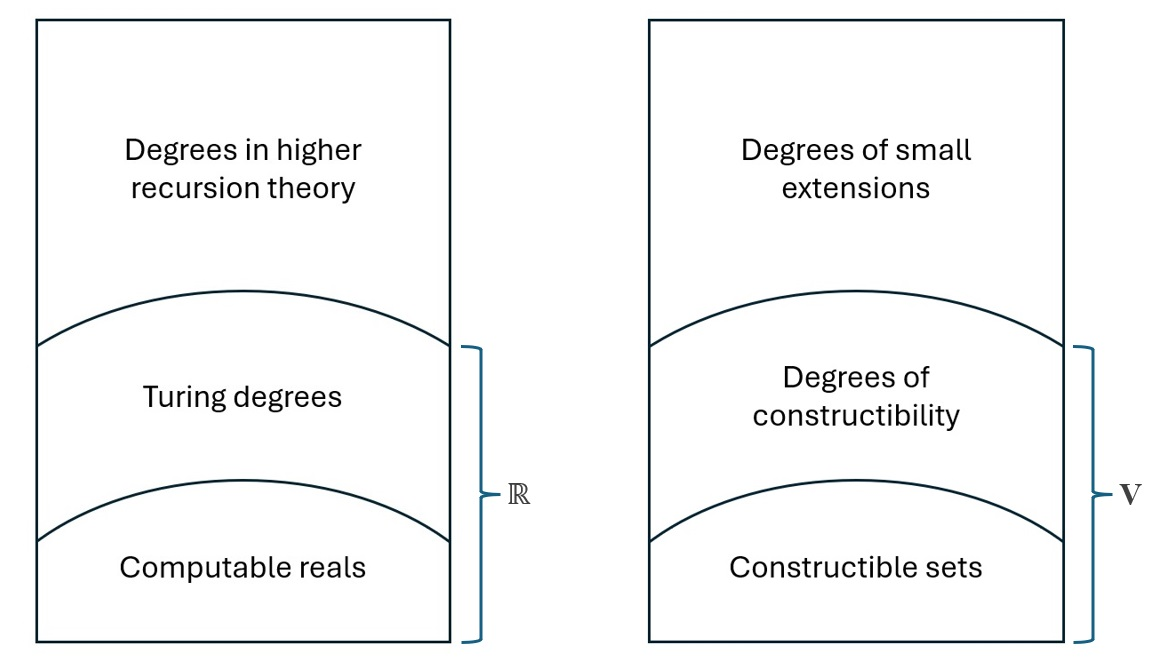
\includegraphics[width=\textwidth]{analogy.jpg}
    \captionsetup{width=0.8\textwidth, format=hang}
    \caption[Comparison between conventional and generalised notions of relative computability]{Comparison between conventional notions of relative computability (left) and our generalised notions (right).}
    \label{analogy}
\end{figure}

Next, we wish to examine (necessarily non-constructive) methods of definably ``accessing'' small extensions of $V$ within $V$, or local methods in short. Set forcing is one such method, and a very well-studied one at that. In an application of set forcing, we pick a partially ordered set --- also known as a forcing notion --- $\mathbb{P} \in V$, and use a filter meeting all dense subsets of $\mathbb{P}$ in $V$ --- termed a $\mathbb{P}$-generic filter over $V$ --- to generate an extension of $V$. So the small extensions of $V$ set forcing brings about via $\mathbb{P}$ are precisely those in
\begin{equation*}
    \{V[g] : g \text{ is a } \mathbb{P} \text{-generic filter over } V\} \text{,}
\end{equation*}
a set definable outside $V$ with $\mathbb{P}$ and its dense subsets in $V$ as parameters. Consequently, one can view set forcing as a recipe in $V$ for generating small extensions of $V$ based only on parameters in $V$. The formal treatment of set forcing inspires a list of desiderata for a local method:
\begin{enumerate}[leftmargin=40pt, label=(DA\arabic*)]
    \item\label{da1} it should be definable in $V$,
    \item\label{da2} it should map parameters to descriptions of how those parameters are used to define generators of small extensions, and
    \item\label{da3} the generators it produces should depend locally on the parameters used to define them. 
\end{enumerate}

A convenient realisation at this juncture is that a recipe and its parameters (or equivalently, the two components of \ref{da2}) can be bundled up into a TCI, since TCIs are basically first-order theories endowed with set constraints that may not be first-order expressible. As in the case of models of standard first-order theories, whether a set $X$ is a model of a TCI $\mathfrak{T}$ depends locally on $X$ and $\mathfrak{T}$. Defining a local method through the language of TCIs and their models thus provides immediate guarantee of \ref{da3}, and is appealing in both its brevity and robustness.

Accompanying the formalisation of local methods, ought to be a notion of relative complexity, a measure which can be utilised to check if one local method is ``more complex'' than another. Akin to relative computability, we want to define relative complexity as a transitive binary relation on the class of all local methods. There is actually a straightforward way to do this: we say method $Y$ is more complex than method $X$ iff the small extensions of $V$ picked out by $Y$ are a non-trivial refinement of those picked out by $X$. Connecting the first-order portion of a TCI with the relative complexity relation we defined, leads to the formulation of a complexity hierarchy --- the local method hierarchy --- very much in line with more notable hierarchies in theoretical computer science (e.g. the arithmetical and polynomial hierarchies).

Leveraging on the forcing framework developed in Section \ref{forframe}, we are able to show that the method of set forcing is exactly $\mathsf{\Sigma_1}$ (or equivalently, as we shall see, $\mathsf{\Pi_2}$) in the local method hierarchy. This is the main takeaway of the work presented in the latter part of this chapter. We follow it up with the analysis of certain witnesses to set forcing being at least as complex as $\mathsf{\Pi_2}$.

By applying an analogue of the Cantor-Bendixson derivative on a specific class of forcing notions, we prove that every TCI $\mathfrak{T} \in \mathsf{\Pi_2}$ either singles out $V$ or picks out continuum-many (as evaluated in the meta-theory) small extensions of $V$. The same is long known to be true for forcing notions: a trivial forcing notion gives $V$ as its sole generic extension, whereas a non-trivial one generates continuum-many generic extensions.

One can think of this chapter as both 
\begin{itemize}
    \item a motivation for, as well as 
    \item a philosophically compelling and coherent repackaging of, 
\end{itemize}
many of the ideas central to Chapter \ref{TCIsec}. 

\section{Degrees of Small Extensions}\label{sect3}

Extending a structure through means of adjoining ``new'' objects is commonly seen in mathematics. Here, ``new'' just means ``existing outside of the structure in question''. For example, a standard course in algebra would talk about field extensions the likes of $\mathbb{Q}[\sqrt{2}]$. In set theory, the subjects of study are models of set theory, often models of $\mathsf{ZFC}$. For convenience, we usually assume such models are countable and transitive. If a \emph{countable transitive model of} $\mathsf{ZFC}$ (henceforth, \emph{CTM}) exists, then extensions of it exist, but due to the complicated closure properties required of a model of $\mathsf{ZFC}$, the proof of their existence is much hairier than that of field extensions. 

It turns out that, whenever $U$ is a CTM and $W$ is an extension of $U$, we can always find an extension of $W$ that is generated over $U$ by a ``small set''. Methods of generating such ``small extensions'' include, but are not limited to, set forcing. In this section, we compare the multiverse of small extensions with the \emph{generic multiverse} born from set forcing, under the assumption that both multiverses have the same centre. We also introduce the idea of \emph{theories with constraints in interpretation} (\emph{TCIs}) to set things up for the next section. 

\subsection{Small Extensions as Degrees}

\begin{rem}
We avoid the usual meta-theoretic concerns regarding forcing and the set-theoretic multiverse by working in the theory 
\begin{equation*}
    \mathsf{ZFC} \ + \text{ ``there is a transitive model of } \mathsf{ZFC}\text{''.}
\end{equation*} 
The existence of CTMs can be proven in this theory.
\end{rem}

\begin{defi}
Given $U$ and $W$, we say $U$ is an \emph{inner model} of $W$ (or equivalently, $W$ is a \emph{outer model} of $U$) iff
\begin{enumerate}[label=(\alph*)]
    \item $U$ and $W$ are CTMs,
    \item $U \subset W$, and
    \item $ORD^U = ORD^W$.
\end{enumerate}
\end{defi}

\begin{defi}\label{def913}
Let $W$ be an outer model of $U$. Then $W$ is a \emph{small extension of} $U$ iff for some $x \in W$, $W$ is the smallest CTM $W'$ satisfying
\begin{enumerate}[label=(\alph*)]
    \item $U \subset W'$, and
    \item $x \in W'$.
\end{enumerate}
In this case, we say, equivalently,
\begin{enumerate}[label=(\arabic*)]
    \item $x$ \emph{generates} $W$ \emph{from} $U$, or
    \item $W$ \emph{is a small extension of} $U$ \emph{generated by} $x$, or
    \item $W = U[x]$.
\end{enumerate}
\end{defi}

The following observation is trivial.

\begin{ob}
The binary relations 
\begin{enumerate}[label=(\arabic*)]
    \item ``being an outer model of'', and
    \item ``being a small extension of''
\end{enumerate}
are both transitive.
\end{ob}

We know that certain sets in outer models can always be used to generate small extensions.

\begin{fact}\label{fact34}
Let $W$ be an outer model of $U$, and $x \in \mathcal{P}(y) \cap W$ for some $y \in U$. Then there is a smallest CTM $W'$ satisfying
\begin{enumerate}[label=(\alph*)]
    \item $U \subset W'$, and
    \item $x \in W'$.
\end{enumerate}
In other words, $U[x]$ exists.
\end{fact}

There is a simple and useful characterisation of small extensions of a CTM.

\begin{prop}\label{prop35}
If $W$ is a small extension of $U$, then for some ordinal $\kappa \in U$, $W$ is generated from $U$ by an unbounded subset of $\kappa$. Furthermore, we can choose $\kappa$ such that
\begin{equation*}
    (U; \in) \models \text{``} \kappa \text{ is a cardinal''.}
\end{equation*}
\end{prop}

\begin{proof}
Let $x \in W$ be such that $W = U[x]$. By the proof of Lemma \ref{setcode}, for some cardinal $\kappa \in W$ there is an unbounded subset $c$ of $\kappa$ in $W$ coding $x$. Since $U$ is an inner model of $W$, $\kappa$ is also a cardinal in $U$. By Fact \ref{fact34}, $U[c]$ exists. Now, $U[c] \subset W$ as $c \in W$; but also $W \subset U[c]$ because $c$ can be decoded in $U[c]$ to give $x$ and $W = U[x]$.
\end{proof}

\begin{defi}
Let $U$ be a CTM. The \emph{outward multiverse centred at} $U$ is the set
\begin{equation*}
    \mathbf{M}(U) := \{W : W \text{ is an outer model of } U\} \text{.}
\end{equation*}
The \emph{small outward multiverse centred at} $U$ is the set
\begin{equation*}
    \mathbf{M}_{S}(U) := \{W : W \text{ is a small extension of } U\} \text{.}
\end{equation*}
\end{defi}

Clearly, $\mathbf{M}_{S}(U) \subset \mathbf{M}(U)$. By Jensen's remarkable result on ``coding the universe'' into a real, $\mathbf{M}_{S}(U)$ is not that much smaller than $\mathbf{M}(U)$.

\begin{fact}[Jensen, \cite{jensencoding}]\label{fact37}
Every CTM has an outer model satisfying 
\begin{equation*}
    \text{``} V = L[r] \text{ for some } r \subset \omega \text{''.}
\end{equation*}
\end{fact}

\begin{prop}
Given a CTM $U$, $(\mathbf{M}_{S}(U), \subset)$ is a cofinal subposet of $(\mathbf{M}(U), \subset)$.
\end{prop}

\begin{proof}
Let $W \in \mathbf{M}(U)$. Then by Fact \ref{fact37}, there is $W' \in \mathbf{M}(U)$ such that $W \subset W'$ and $W'$ satisfies
\begin{equation*}
    \text{``} V = L[r] \text{ for some } r \subset \omega \text{''.}
\end{equation*}
Since $L^{W'} = L^U \subset U$ and indeed $W' = L^{W'}[r]$ for some real $r \in W'$ from the outside, necessarily $W' = U[r]$. But this means $W' \in \mathbf{M}_{S}(U)$.
\end{proof}

We can characterise members $\mathbf{M}_{S}(U)$ in a way that is conducive to the discussion of relative computability.

\begin{prop}\label{prop37}
Let $U$ be a CTM. Then
\begin{align*}
    \mathbf{M}_{S}(U) & = \{U[x] : x \in \bigcup \mathbf{M}(U) \cap \mathcal{P}(U)\} \\
    & = \{U[x] : x \in \bigcup \mathbf{M}(U) \cap \mathcal{P}(ORD^U)\} \text{.}
\end{align*}
\end{prop}

\begin{proof}
By Fact \ref{fact34} and Proposition \ref{prop35}.
\end{proof}

Proposition \ref{prop37} gives us a natural reducibility relation on 
\begin{equation*}
    \mathbf{N}(U) := \bigcup \mathbf{M}(U) \cap \mathcal{P}(ORD^U)
\end{equation*}
given a CTM $U$. 

\begin{defi}\label{def9111}
Let $U$ be a CTM. Define the binary relation $\leq_U$ on $\mathbf{N}(U)$ as follows: for $x, y \in \mathbf{N}(U)$,
\begin{equation*}
    x \leq_U y \iff U[x] \subset U[y] \text{.}
\end{equation*}
Given $x, y \in \mathbf{N}(U)$, write $x \equiv_U y$ iff $x \leq_U y$ and $y \leq_U x$.
\end{defi}

One can easily check that $\leq_U$ is a preorder, so taking its quotient by $\equiv_U$ results in a partial order we shall denote as $(\mathcal{D}(U), \leq_{\mathcal{D}(U)})$.

The case of $(\mathcal{D}(U), \leq_{\mathcal{D}(U)})$ parallels that of the constructibility degrees, in the sense that the former partial order, like the latter one, is isomorphic to a class of set-theoretic universes under inclusion. Specifically, 
\begin{equation*}
   (\mathcal{D}(U), \leq_{\mathcal{D}(U)}) \cong (\mathbf{M}_S(U), \subset) \text{.} 
\end{equation*} 
This motivates viewing $(\mathcal{D}(U), \leq_{\mathcal{D}(U)})$ as degrees of generalised computability over $U$. These degrees are necessarily non-constructible (and indeed, non-constructive) without full access to $U$, if $U$ is not a model of ``$V = L$''. Whereas the ``constructible in'' relation partially orders a partition of an $\in$-model of $\mathsf{ZFC}$ and is definable within said model, the field of $(\mathcal{D}(U), \leq_{\mathcal{D}(U)})$ may not be realisable as a partition of any such model. We thus expect the structure of $(\mathcal{D}(U), \leq_{\mathcal{D}(U)})$ to be much more varied and dependent on $U$, compared to the structure of the constructibility degrees evaluated in $U$. Nevertheless, we will attempt to stratify $(\mathcal{D}(U), \leq_{\mathcal{D}(U)})$.

\begin{rem}\label{rem9112}
The labelling of $(\mathcal{D}(U), \leq_{\mathcal{D}(U)})$ as degrees of generalised computability over $U$ hints at $U$ being some sort of abstract non-deterministic generalised computer that always returns the equivalence class of its input under $\equiv_U$. 

Often, a model of (relative) computation is presented in abstract terms as a definable set of ``computers''. An obvious example: Turing machines, as a model of computation, is the set of all Turing machines. Adopting this notion, we are then justified to think of $U$ as the sole exemplar of the model of relative computation which gives rise to the degree structure $(\mathcal{D}(U), \leq_{\mathcal{D}(U)})$.
\end{rem}

Hereon, we shall analyse and reason about $(\mathcal{D}(U), \leq_{\mathcal{D}(U)})$ by identifying it with $(\mathbf{M}_S(U), \subset)$, so that we can apply set-theoretic arguments and leverage on set-theoretic techniques.

\subsection{The Generic Multiverse}\label{genmul}

The generic multiverse, first coined by Woodin in \cite{woodingen} as a collection of universes of set theory 
\begin{quote}
    ``[closed] under generic extensions (enlargements) and under generic re nements (inner models of a universe which the given universe is a generic extension of)'',
\end{quote}
caught on as a popular subject of study in set theory in the recent decade or so, especially by Hamkins, Friedman, et al. (See e.g. \cite{hamkinsmoving} and \cite{sygeneric}.) As we shall see, there are good reasons for viewing generic multiverses as relatively well-understood analogues of multiverses of small extensions.

In this subsection, comparisons are made between the outward generic multiverse and the small outward multiverse. In particular, simple properties of the outward generic multiverse as a suborder of the small outward multiverse are proven.

\begin{defi}
Define the relation $\leq_F$ on the set of CTMs as follows:
\begin{equation*}
    M \leq_F N \iff N \text{ is a forcing extension of } M \text{.}
\end{equation*}
\end{defi}

\begin{defi}
A \emph{(full) generic multiverse} is any set of CTMs closed under $\leq_F$.
\end{defi}

\begin{defi}
Let $V$ be a CTM. The \emph{(forcing) grounds of} $V$ is the set
\begin{equation*}
    \{W : V \text{ is a forcing extension of } W\} \text{.}
\end{equation*}
\end{defi}

\begin{defi}\label{def9116}
Let $V$ be a CTM. The \emph{outward generic multiverse centred at} $V$ is the set
\begin{equation*}
    \mathbf{M}_F(V) := \{W : W \text{ is a forcing extension of } V\} \text{.}
\end{equation*}
\end{defi} 

Much has been studied about the structure of standard generic multiverses under $\leq_F$, with a particularly strong focus on the forcing grounds of fixed CTMs. On the other hand, there has been less interest in the structure of outward generic multiverses under $\leq_F$, perhaps due to the dearth of low-hanging fruits --- a large part of what is known about this structure are essentially theorems about forcing in the traditional sense.

A careful reader might have noticed the overloading of the notation $\cdot [\cdot]$ to represent both small extensions and forcing extensions. This is intentional, for the latter class is subsumed under the former.

\begin{fact}
For some $\mathbb{P} \in V$, let $g$ be a $\mathbb{P}$-generic filter over a CTM $V$. Then $V[g]$ is the smallest CTM $W$ for which
\begin{enumerate}[label=(\alph*)]
    \item $V \subset W$, and
    \item $g \in W$.
\end{enumerate}
As a consequence, $\mathbf{M}_F(V) \subset \mathbf{M}_S(V)$.
\end{fact}

It turns out that forcing extensions of a CTM $V$ are downward-closed in $\mathbf{M}(V)$ (and thus, also in $\mathbf{M}_S(V)$). This is just a rephrasing of the fact below.

\begin{fact}\label{fact221}
Let $V \subset U \subset W$ be CTMs such that
\begin{itemize}
    \item $W$ is a forcing extension of $V$, 
    \item $U$ is an outer model of $V$, and
    \item $U$ is an inner model of $W$.
\end{itemize}
Then 
\begin{enumerate}[label=(\alph*)]
    \item $U$ is a forcing extension of $V$, and
    \item $W$ is a forcing extension of $U$.
\end{enumerate}
\end{fact}

An immediate follow-up question to the previous two facts is, 
\begin{quote}
    ``Must $\mathbf{M}_F(V)$ always equal $\mathbf{M}_S(V)$?''
\end{quote}
There is an easy argument for the answer being ``no'', if we assume a sufficiently strong large cardinal axiom in addition to $\mathsf{ZFC}$.

\begin{prop}\label{prop318}
Let 
\begin{equation*}
    \mathsf{T} := \mathsf{ZFC} + \text{``}0^{\sharp}\text{ exists''.}
\end{equation*} 
Assume $\mathsf{ZFC} + \text{``there is a transitive model of } T \text{''}$. Then $\mathbf{M}_F(V) \subsetneq \mathbf{M}_S(V)$ for some CTM $V$.
\end{prop}

\begin{proof}
Given the hypothesis of the proposition, there is a CTM $W$ satisfying $\mathsf{T}$. Define 
\begin{gather*}
    V := L^W \\
    U := L[I]^W \text{,}
\end{gather*}
where $I$ is an uncountable set of Silver indiscernibles in $W$ witnessing the fact that $0^{\sharp}$ exists. Then $U$ is a small extension of $V$ generated by $I \in U$ but not a forcing extension of $V$.
\end{proof}

By Proposition \ref{prop318}, it is consistent that $\mathbf{M}_S(V) \setminus \mathbf{M}_F(V)$ is non-trivial --- and includes at least a cone of $(\mathbf{M}_S(V), \subset)$ --- under strong enough assumptions. However, the small outward multiverse example exhibited by the proof of the proposition is undesirable because it is centred at a universe that is by many measures, ``too small'' (e.g. it has a trivial theory of constructibility degrees). 

A much stronger and much more useful statement would be
\begin{equation}\label{eq31p}
    \text{``} \mathbf{M}_F(V) \neq \mathbf{M}_S(V) \text{ for all } V \text{''.}
\end{equation}
Let us sketch how this can be true. We start with a universe $V$, force (with a proper class forcing notion) to an outer model $V[G]$ of $V$ satisfying ``$V[G]$ is not a set forcing extension of $V$'', then apply Fact \ref{fact37} to $V[G]$. The end result is an outer model $W$ of $V[G]$ such that $W = L^V[r]$ for some real $r \in W$. This can even be arranged such that $V$ is a definable class in $W$. Now if $W$ is a set forcing extension of $V$, then so are all intermediate outer models of $V$, including $V[G]$. But we have just ensured $V[G]$ is not a set forcing extension of $V$. 

This argument, which includes a proof of Fact \ref{fact37}, can be formalised in a conservative second order extension of $\mathsf{ZFC}$ (the second-order portion is needed for proper class forcing), so our meta-theory suffices when $V$ is a CTM. We have thus established --- albeit sketchily so --- the following.

\begin{fact}\label{fact319}
(\ref{eq31p}) holds.
\end{fact}

In actuality, we can switch $V$ for any $U \in \mathbf{M}_S(V)$ in the argument above and obtain a stronger conclusion.

\begin{fact}\label{fact229}
Given a CTM $V$,
\begin{equation*}
    (\mathbf{M}_S(V) \setminus \mathbf{M}_F(V), \subset)
\end{equation*}
is a cofinal subposet of $(\mathbf{M}_S(V), \subset)$.
\end{fact}

Intuitively, Facts \ref{fact221} and \ref{fact229} tell us that there are many objects inaccessible by forcing. Do these objects have ``local first-order properties'' not shared by any set in any forcing extension? We shall aim to partially answer this question, through applications of the tools we built in Part \ref{part2}.

\section{Local Method Definitions}

If we look at forcing as a way to uniformly describe by intension members of a subset of $\mathbf{N}(V)$ for some CTM $V$, where the evaluation of intension is done outside $V$, then we quickly realise that said description can be very simple. We essentially just 
\begin{itemize}
    \item shortlist a class of structures in $V$ --- forcing notions augmented with predicates for their dense subsets --- and
    \item describe how we pick substructures --- generic filters --- of these structures outside $V$. 
\end{itemize} 
Note also that the description of each substructure $\mathfrak{A}'$ involves only information about its associated superstructure $\mathfrak{A}$, so we expect every reasonable universe containing $\mathfrak{A}$ to see that $\mathfrak{A}'$ fits the description. This is analogous to (albeit stronger than) the kind of local definablity one would expect the state transition function of a typical machine model of computation to satisfy.

\subsection{Locally Definable Methods of Small Extensions}

This idea of generating new structures outside the universe based locally on recipes defined in the universe can be formalised rather conveniently using the language of TCIs. 

\begin{defi}\label{def320}
Let $V$ be a CTM. A set $X \subset V$ is a $\mathbf{M}_S(V)$ \emph{method definition of small extensions} (henceforth, $\mathbf{M}_S(V)$ \emph{method definition}) iff it is non-empty and contains only TCIs.
\end{defi}

\begin{defi}\label{def323}
If $V$ is a CTM and $\mathfrak{T} \in V$ is a TCI, then the \emph{evaluation of} $\mathfrak{T}$, denoted $\mathrm{Eval}^V(\mathfrak{T})$, is the set
\begin{equation*}
    \{V[\mathcal{M}] : \exists W \ \exists \mathcal{M} \ (W \in \mathbf{M}(V) \wedge \mathcal{M} \in W \wedge \mathcal{M} \models^* \mathfrak{T})\} \text{.}
\end{equation*}
\end{defi}

\begin{defi}\label{def923}
Let $V$ be a CTM. A set $X \subset V$ is a $\mathbf{M}_S(V)$ \emph{local method definition of small extensions} (henceforth, $\mathbf{M}_S(V)$ \emph{local method definition}) iff it is a $\mathbf{M}_S(V)$ method definition and $X$ is definable (possibly as a proper class) in $V$ with parameters in $V$. 
\end{defi}

\begin{rem}\label{rem924}
We can think of any TCI as an abstract generalised computer that works \emph{a priori} independently of $V$ (see Remark \ref{rem9112} for an argument for $V$ being an abstract computer). This is akin to how a pairing of an oracle machine and a set of natural numbers to be used as oracle, is an abstract computer. For instance, given an oracle machine $\Phi$ and a set $A \subset \omega$, $\Phi$ with $A$ as oracle computes some set of natural numbers $B$, in the sense that $\Phi^A = B \subset \omega$. Analogously, the models of a TCI over all outer models of $V$ are the possible sets it can ``compute''. These models are generally not unique due to the non-constructive nature of objects outside $V$. As a result, the ``computations'' carried out by non-trivial TCIs are inherently fuzzy.

Just like how a set computed by some oracle machine with a fixed oracle --- or indeed, a set defined by some formula in the language of arithmetic --- can be used to pick out a Turing degree, we want to have a TCI in $V$ pick out a degree of small extension of $V$. However, just as we do not expect a non-trivial TCI to ``deterministically compute'' a single set, we should also not expect it to isolate a single such degree, due to the outer models themselves being non-constructive. Consequentially, there is also no avoiding fuzziness when we evaluate TCIs to obtain degrees. This is the intuition behind $\mathrm{Eval}^V$ taking TCIs to subsets of $\mathbf{M}_S(V)$, instead of taking TCIs to points in $\mathbf{M}_S(V)$.
\end{rem}

It might not be immediately obvious that whenever there are $W$ and $\mathcal{M}$ for which $\mathcal{M} \in W \in \mathbf{M}(V)$ and $\mathcal{M} \models^* \mathfrak{T}$ for some TCI $\mathfrak{T} \in V$, $V[\mathcal{M}]$ must exist. The next proposition, summarising much of the setup done in Section \ref{GOCon}, shows that one can translate between models of a TCI $\mathfrak{T}$ and subsets of a set associated with $\mathfrak{T}$. Further, this translation can be carried out in an absolute and uniform manner.

\begin{prop}\label{prop322}
There are formulas $\phi$ and $\psi$ in the language of set theory with the following properties: 
\begin{enumerate}[label=(\arabic*)]
    \item $\phi$ and $\psi$ have two and three free variables respectively,
    \item $\phi$ defines a function from the class of all TCIs into the universe,
    \item $\psi$ defines a function from the class
    \begin{equation*}
        \{(\mathfrak{T}, \mathcal{M}) : \mathfrak{T} \text{ is a TCI and } \mathcal{M} \models^* \mathfrak{T}\}
    \end{equation*}
    into the universe,
    \item $\phi$ and $\psi$ are absolute for transitive models of $\mathsf{ZFC}$,
    \item\label{3245} whenever $\mathfrak{T}$ is a TCI, the relation
    \begin{equation*}
        R_{\mathfrak{T}} := \{(\mathcal{M}, x) : \psi(\mathfrak{T}, \mathcal{M}, x)\}
    \end{equation*}
    is one-one, 
    \item\label{3246} for all $\mathfrak{T}$, $\mathcal{M}$ and $x$, $\psi(\mathfrak{T}, \mathcal{M}, x)$ implies there is $\mathcal{L}$ for which $\phi(\mathfrak{T}, \mathcal{L})$ and $x \subset \mathcal{L}$, and
\end{enumerate}
\end{prop}

In the presence of Fact \ref{fact34}, Proposition \ref{prop322} gives validity to Definition \ref{def323}: the function $\mathrm{Eval}^V$ taking TCIs in $V$ to subsets of $\mathbf{M}_S(V)$ actually exists. Fix formulas $\phi$ and $\psi$ as in Proposition \ref{prop322}. Let 
\begin{align*}
    \mathcal{L}_{\mathfrak{T}} := \ & \text{ the unique } \mathcal{L} \text{ for which } \phi(\mathfrak{T}, \mathcal{L}) \text{, and} \\
    \Sigma(\mathfrak{T}, \mathcal{M}) := \ & \text{ the unique } x \text{ for which } \psi(\mathfrak{T}, \mathcal{M}, x) \text{.}
\end{align*}
Given a TCI $\mathfrak{T} = (T, \sigma, \dot{\mathcal{U}}, \vartheta)$ and sets $y, z$ with $\vartheta(\dot{\mathcal{U}}) = (y, z)$, we should think of $\mathcal{L}_{\mathfrak{T}}$ as containing all the possible atomic sentences over $\sigma$ that involve members of $y$ as parameters. Then for any model $\mathcal{M}$ of $\mathfrak{T}$, $\Sigma(\mathfrak{T}, \mathcal{M})$ ($\subset \mathcal{L}_{\mathfrak{T}}$, by \ref{3246} of Proposition \ref{prop322}) can be thought of as the ``$\mathfrak{T}$-specific atomic diagram''  of $\mathcal{M}$. According to \ref{3245} of Proposition \ref{prop322}, we can always recover $\mathcal{M}$ in a transitive model of $\mathsf{ZFC}$ from $\mathfrak{T}$ and $\Sigma(\mathfrak{T}, \mathcal{M})$ alone. As a consequence, 
\begin{equation*}
    V[\mathcal{M}] = V[x] \text{ if } V \text{ is a CTM and } \psi(\mathfrak{T}, \mathcal{M}, x) \text{ for some TCI } \mathfrak{T} \in V \text{.}
\end{equation*}

Observe that we can ``cover'' the entire small outward multiverse with a local method definition.

\begin{prop}\label{prop326}
Let $V$ be a CTM. There is a $\mathbf{M}_S(V)$ local method definition $X$ containing only $\Pi_0$ ($= \Sigma_0$) TCIs such that 
\begin{equation*}
    \bigcup \ ((\mathrm{Eval}^V)" X) = \mathbf{M}_S(V) \text{.}
\end{equation*}
\end{prop}

\begin{proof}
Fix a distinguished unary relation symbol $\dot{\mathcal{U}}$ and let $s \in V$. Define 
\begin{gather*}
    \vartheta_s := \{(\dot{\mathcal{U}}, (s, 0))\} \\
    \mathfrak{T}_s := (\emptyset, \emptyset, \dot{\mathcal{U}}, \vartheta_s) \text{.}
\end{gather*}
Then $\mathfrak{T}_s$ is a $\Pi_0$ TCI, and its models in any outer model $W$ of $V$ are exactly the subsets of $s$ in $W$. We are done by Fact \ref{fact34} if we set $X := \{\mathfrak{T}_s : s \in V\}$.
\end{proof}

To kickstart our journey of formally relating set-theoretic forcing to TCIs, as promised at the end of Section \ref{GOCon}, some recollection is in order. First, recall from Section \ref{GOCon}, 
\begin{itemize}
    \item the abbreviation
    \begin{equation*}
        \mathfrak{A}_{\mathfrak{T}} := (H(|trcl(\mathfrak{T})|^+); \in) \text{,}
    \end{equation*}
    \item Definition \ref{def4212}, and 
    \item Observation \ref{smallvgen}.
\end{itemize}

\begin{ob}\label{ob331}
It is easily verifiable from the definitions of $\mathcal{L}_{\mathfrak{T}}$ and $\mathfrak{A}_{\mathfrak{T}}$ that $\mathcal{L}_{\mathfrak{T}} \in \mathfrak{A}_{\mathfrak{T}}$, so we have $[\mathcal{L}_{\mathfrak{T}}]^{< \omega} \in \mathfrak{A}_{\mathfrak{T}}$ as well.
\end{ob}

Next, recall that by Lemma \ref{gmodelsinfe}, $V$-generic models of a TCI $\mathfrak{T}$ are exactly the models of $\mathfrak{T}$ found in some forcing (i.e. generic) extension of $V$.

Finally, recalling Theorem \ref{revgenmodels}, we wrap up this subsection by demonstrating that forcing can be regarded as a local method definition.

Unless stated otherwise, we work within a fixed CTM $V$ for the rest of this section, so that all mentions of $\mathbf{M}_S(V)$ in (local) method definitions can be conveniently suppressed.

Now, the gist of Theorem \ref{revgenmodels} can be rephrased as the following proposition.

\begin{prop}\label{prop323}
Let $\mathbb{P} = (P, \leq_{\mathbb{P}})$ be a partial order. Then there is a TCI $\mathfrak{T}(\mathbb{P}) = (T, \sigma, \dot{\mathcal{U}}, \vartheta)$ such that for a fixed unary relation symbol $\dot{X} \in \sigma$, if $\mathcal{M}$ is any set in an outer model of $V$, then
\begin{equation*}
    \mathcal{M} \models^* \mathfrak{T}(\mathbb{P}) \iff \{p : \mathcal{M} \models \dot{X}(p)\} \text{ is a } \mathbb{P} \text{-generic filter over } V \text{.}
\end{equation*}
\end{prop}

\begin{cor}\label{cor324}
Forcing is expressible as a local method definition.
\end{cor}

\begin{proof}
The proof of Theorem \ref{revgenmodels} (and thus of Proposition \ref{prop323}) is constructive, and can be made uniform across all possible $\mathbb{P}$ by choosing the symbols $\dot{\mathcal{U}}$, $\dot{\leq}$ and $\dot{G}$ in advance. This allows the function 
\begin{equation*}
    (F : \{\text{forcing notions}\} \longrightarrow V) [\mathbb{P} \mapsto \mathfrak{T}(\mathbb{P})]
\end{equation*}
to be definable in $V$. Obviously, $dom(F)$ is definable in $V$, so $ran(F)$ must be as well. 
\end{proof}

Let us choose a definable function $F$ as in the proof of Corollary \ref{cor324} and name it $\mathfrak{T}(\cdot)$, for later use and reference. Also, we shall use $\mathsf{Fg}$ to denote the local method definition of forcing; in other words,  $\mathsf{Fg} := ran(\mathfrak{T}(\cdot))$.

\subsection{Complexity of Local Method Definitions}\label{ss32}

What does it mean for a definition to be complex? Long, overwrought, convoluted. These are just some synonyms that may come to mind. in general, a more complex definition places more requirements on the object, or the class of objects, it defines. In the former scenario, it makes the object it defines \textit{a priori} less likely to exist; in the latter one, it defines a compratively smaller class of objects. Following this intuition, we formalise a way of comparing between two local method definitions.

\begin{defi}\label{def9210}
Let $X, Y$ be local method definitions of a CTM $V$. We use 
\begin{enumerate}[label=(\arabic*)]
    \item $X \leq^M_w Y$ to denote the statement
    \begin{gather*}
        \text{``for each consistent } \mathfrak{T} \in X \text{ there is } \mathfrak{T}' \in Y \text{ such that} \\
        \emptyset \neq \mathrm{Eval}^V(\mathfrak{T}') \subset \mathrm{Eval}^V(\mathfrak{T}) \text{'',}
    \end{gather*}
    and
    \item $X \leq^M Y$ to denote the statement
    \begin{align*}
        \text{``} & \text{there is a function } F : X \longrightarrow Y \text{ definable in } V \text{ such that} \\ 
        & \emptyset \neq \mathrm{Eval}^V(F(\mathfrak{T})) \subset \mathrm{Eval}^V(\mathfrak{T}) \text{ for all consistent } \mathfrak{T} \in X \text{''.}
    \end{align*}
    When said statement is true, we say $F$ \emph{witnesses} $X \leq^M Y$.
\end{enumerate}
\end{defi}

\begin{defi}
Let $X, Y$ be local method definitions. We say
\begin{enumerate}[label=(\arabic*)]
    \item $X \equiv^M_w Y$ iff $X \leq^M_w Y$ and $Y \leq^M_w X$,
    \item $X \equiv^M Y$ iff $X \leq^M Y$ and $Y \leq^M X$,
    \item $X <^M_w Y$ iff $X \leq^M_w Y$ and $Y \not\leq^M_w X$, and
    \item $X <^M Y$ iff $X \leq^M Y$ and $Y \not\leq^M X$.
\end{enumerate}
\end{defi}

\begin{ob}
\leavevmode
\begin{enumerate}[label=(\arabic*)]
    \item $\leq^M_w$ and $\leq^M$ are transitive relations, so $\equiv^M_w$ and $\equiv^M$ are equivalence relations.
    \item $\leq^M_w$ and $\leq^M$, as subclasses of $V$, are only definable outside $V$, for their definitions require quantification over proper subclasses of $V$. 
    \item Obviously, $X \leq^M Y$ always implies $X \leq^M_w Y$, so $\leq^M_w$ is weaker than $\leq^M$. 
\end{enumerate}
\end{ob}

Intuitively, $Y$ is more complex than $X$ as a definition when $X \leq^M_w Y$ or $X \leq^M Y$, because $Y$ both refines and extends $X$. Refinement occurs because no matter set a description of $X$ picks out, $Y$ contains a description that picks out a smaller non-empty set. Extension occurs because $Y$ may have a description pick out a set that is not covered by any description of $X$. The difference between the two relations then boils down to whether a witness to said refinement and extension exists in $V$.

Figure \ref{intuition} provides one way of visualising $X \leq^M Y$ with witness function $F$.

\begin{figure}[!ht]
    \centering
    \centerline{\hspace{1pt}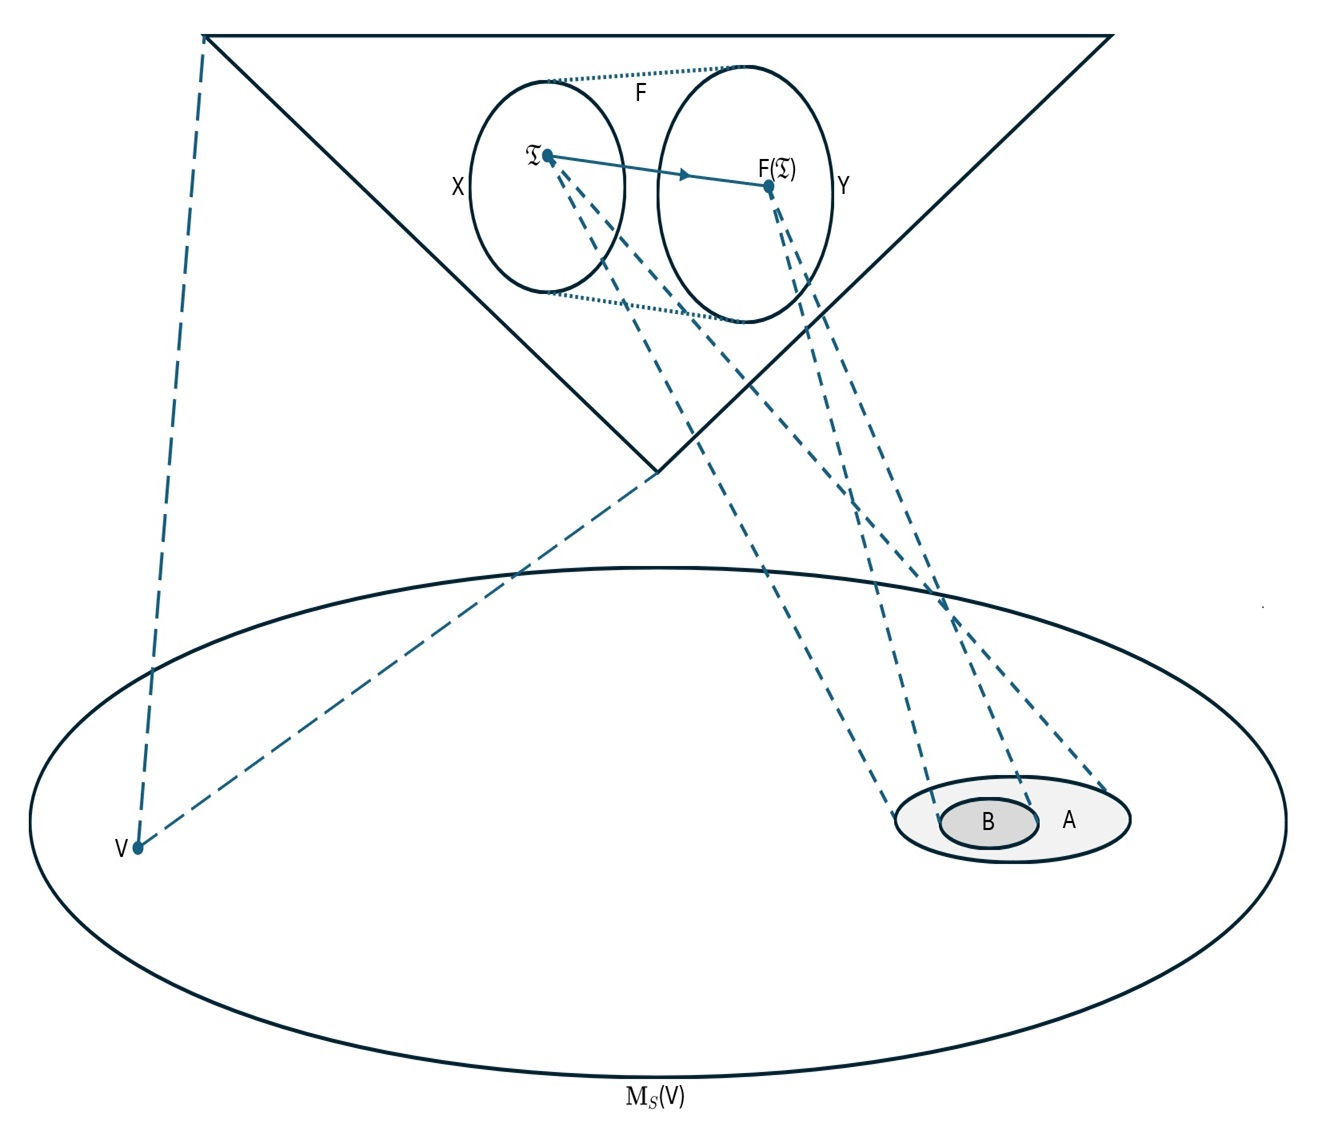
\includegraphics[width=1.05\textwidth]{intuition.jpg}}
    \captionsetup{width=0.8\textwidth, format=hang}
    \caption[Visual representation of a function $F$ witnessing $X \leq^M Y$]{Visual representation of a function $F$ witnessing $X \leq^M Y$, where $X$ and $Y$ are local method definitions. \\ Here, $\mathfrak{T}$ is an arbitrary consistent member of $X$, and \\ $B = \mathrm{Eval}^V(F(\mathfrak{T})) \subset \mathrm{Eval}^V(\mathfrak{T}) = A$.}
    \label{intuition}
\end{figure}

\begin{rem}
Since a model of computation is just a definable set of ``computers'' (as echoed in Remark \ref{rem9112}), it makes sense to view a local method definition $X$ as an abstract model of generalised computation definable in $V$. In this perspective, the following are straightforward implications.
\begin{enumerate}[label=(\arabic*)]
    \item The collection of sets of degrees
    \begin{equation*}
        \{\mathrm{Eval}^V(\mathfrak{T}) : \mathfrak{T} \in X\}
    \end{equation*}
    is precisely the collection of ``fuzzy'' (in the sense elaborated on in Remark \ref{rem924}) degrees picked out by instances of model $X$. This is analogous to the collection of Turing degrees picked out by a definable set of machine-oracle pairs --- for example, the set of Turing degrees picked out by pairing one particular oracle machine with all subsets of $\omega$.
    \item The relations $\leq^M_w$ and $\leq^M$ are designed to compare the complexity between models of computation definable in $V$, after they are uniformly augmented with the computational power of $V$ itself (see Remark \ref{rem9112} again).
\end{enumerate}  

Note that if the degrees picked out by evaluating TCIs were not ``fuzzy'' , then no proper refinement would ever occur, and our interpretations of $\leq^M_w$ and $\leq^M$ would naturally simplify to various extents of ``less powerful''. This suggests that our notions of relative complexity generalise the conventional notions of relative computational power.
\end{rem}

It would be good if $V$ can decide (albeit not uniformly) whether $X \leq^M Y$ for arbitrary local method definitions $X$ and $Y$. Unfortunately, there seems to be no straightforward indication of that: it is not clear if $V$ is always privy to proof of $X \leq^M Y$. For certain pairs $(X, Y)$ though, $X \leq^M Y$ is provable in $\mathsf{ZFC}$, and so $V$ must know it is true.

\begin{prop}\label{prop338}
Let $X, Y$ be local method definitions. If $X \subset Y$, then $X \leq^M Y$.
\end{prop}

\begin{proof}
The identity map on $X$ is definable in $V$ and witnesses $X \leq^M Y$.
\end{proof}

\begin{prop}
There is a greatest local method definition with respect to $\leq^M$.
\end{prop}

\begin{proof}
Let $Y$ be the class of all TCIs. Clearly $Y$ is a local method definition. Moreover, $X \subset Y$ for every local method definition $X$. By Proposition \ref{prop338}, $X \leq^M Y$ for every local method definition $X$.
\end{proof}

\begin{prop}
A local method definition is not smallest with respect to $\leq^M$ iff it contains a consistent TCI.
\end{prop}

\begin{proof}
Clearly, every local method definition containing no consistent TCIs is smallest with respect to $\leq^M$. For the converse, by Proposition \ref{prop326}, it suffices to show that for every $x \in V$, there is a small extension of $V$ not generated by a subset of $x$. But this is implied by the forcing notion $Col(|x|^+, |x|^+)^V$ adding no subsets of $x$ over $V$.
\end{proof}

We now define a natural hierarchy on the class of TCIs.

\begin{defi}\label{def339}
For $n < \omega$, we have the following local method definitions:
\begin{align*}
    \mathsf{\Pi^M_n} := \ & \{\mathfrak{T} : \mathfrak{T} \text{ is a } \Pi_n \text{ TCI}\}
    \\
    \mathsf{\Sigma^M_n} := \ & \{\mathfrak{T} : \mathfrak{T} \text{ is a } \Sigma_n \text{ TCI}\} \text{.}
\end{align*}
\end{defi}

\begin{prop}\label{prop340}
Let $n < \omega$. Then
\begin{enumerate}[label=(\arabic*)]
    \item $\mathsf{\Pi^M_n} \leq^M \mathsf{\Pi^M_{n+1}}$,
    \item $\mathsf{\Sigma^M_n} \leq^M \mathsf{\Sigma^M_{n+1}}$,
    \item $\mathsf{\Pi^M_n} \leq^M \mathsf{\Sigma^M_{n+1}}$, and
    \item $\mathsf{\Sigma^M_n} \leq^M \mathsf{\Pi^M_{n+1}}$.
\end{enumerate}
\end{prop}

\begin{proof}
By Proposition \ref{prop338}.
\end{proof}

By Proposition \ref{prop340}, 
\begin{equation*}
    \{\mathsf{\Pi^M_n} : n < \omega\} \cup \{\mathsf{\Sigma^M_n} : n < \omega\}
\end{equation*}
forms a hierarchy of local method definitions with $\leq^M$-predecessor sets that grow with $n$. We shall call this the \emph{local method hierarchy}.

Mathematics and computer science are replete with hierarchies similar to the local method hierarchy, where syntactic forms of defining formulas are used to categorise sets. Examples include the projective, arithmetical and polynomial hierarchies. If we think of TCIs as augmentations of first-order theories with added constraints that are bounded but not first-order definable, then the local method hierarchy segregates TCIs based only on their first-order parts.

It turns out that most of the $\mathsf{\Pi^M_n}$'s are unnecessary in this hierarchy. 

\begin{thm}\label{prop252'}
Let $n$ satisfy $1 \leq n < \omega$. For every $\mathfrak{T} \in \mathsf{\Pi^M_{n+1}}$ there are
\begin{enumerate}[label=(\arabic*)]
    \item $\mathfrak{T}' \in \mathsf{\Sigma^M_n}$, and
    \item a formula $\theta$ with two free variables,
\end{enumerate}
such that 
\begin{enumerate}[label=(\alph*)]
    \item $\theta$ is absolute for outer models of $V$, and
    \item in every outer model of $V$, $\theta$ defines a bijection from the set of models of $\mathfrak{T}$ into the set of models of $\mathfrak{T}'$.
\end{enumerate}
\end{thm}

\begin{proof}
Let 
\begin{itemize}
    \item $1 \leq n < \omega$,
    \item $\mathfrak{T}  = (T, \sigma, \dot{\mathcal{U}}, \vartheta) \in \mathsf{\Pi^M_{n+1}}$, and 
    \item $\vartheta(\dot{\mathcal{U}}) = (y, z)$.
\end{itemize} 
We shall first construct $\mathfrak{T}' \in \mathsf{\Sigma^M_n}$ from $\mathfrak{T}$. Expand the signature $\sigma$ to $\sigma'$ by adding 
\begin{itemize}
    \item a unary relation symbol $\dot{T}$, as well as
    \item a constant symbol $\dot{c}$ for each $c \in y$, 
\end{itemize}
all of which are new to $\sigma$ and distinct from one another. Define $\vartheta'$ point-wise as follows:
\begin{gather*}
    \vartheta'(\dot{\mathcal{U}}) := (y, 1) \\
    \vartheta'(\dot{X}) := (y', 0) \text{ whenever } \dot{X} \in \sigma \text{ and } \vartheta(\dot{X}) = (y', z') \\
    \vartheta'(\dot{T}) := (y, z) \\
    \vartheta'(\dot{c}) := (\{c\}, 0) \text{ for all } c \in y \text{.}
\end{gather*}

Next, initialise $T^*$ to be 
\begin{align*}
    T & \cup \{\ulcorner \forall x_1 \dots \forall x_k \ \exists x_{k+1} \ (\dot{F}(x_1, \dots, x_k) = x_{k+1}) \urcorner \\
    & \mspace{25mu} : \dot{F} \in \sigma \text{ is a } k \text{-ary function symbol}\} \text{.}
\end{align*}
For each $\dot{X} \in \sigma$, so that $\vartheta(\dot{X})$ is of the form $(y', z')$, do the following.
\begin{enumerate}[label=Case (\arabic*)$_{\dot{X}}$:, leftmargin=70pt]
    \item $\dot{X}$ is a $k$-ary function symbol. Without loss of generality, we can assume $y' \subset y^{k+1}$. Add to $T^*$ every member of the set
    \begin{align*}
        \{ & \ulcorner \dot{X}(\dot{c}_1, \ldots, \dot{c}_k) = \dot{c}_{k+1} \implies \dot{T}(\dot{c}_1) \wedge \ldots \wedge \dot{T}(\dot{c}_{k+1}) \urcorner \\
        & : (c_1, \ldots, c_{k+1}) \in y'\} \text{.}
    \end{align*}
    If in addition, $z' = 1$, then also add to $T^*$ every member of the set
    \begin{align*}
        \{ & \ulcorner \dot{T}(\dot{c}_1) \wedge \ldots \wedge \dot{T}(\dot{c}_{k+1}) \implies \dot{X}(\dot{c}_1, \ldots, \dot{c}_k) = \dot{c}_{k+1} \urcorner \\
        & : (c_1, \ldots, c_{k+1}) \in y'\} \text{.}
    \end{align*}
    \item $\dot{X}$ is a $k$-ary relation symbol. Without loss of generality, we can assume $y' \subset y^k$. Add to $T^*$ every member of the set
    \begin{align*}
        \{ & \ulcorner \dot{X}(\dot{c}_1, \ldots, \dot{c}_k) \implies \dot{T}(\dot{c}_1) \wedge \ldots \wedge \dot{T}(\dot{c}_k) \urcorner \\
        & : (c_1, \ldots, c_k) \in y'\} \text{.}
    \end{align*}
    If in addition, $z' = 1$, then also add to $T^*$ every member of the set
    \begin{align*}
        \{ & \ulcorner \dot{T}(\dot{c}_1) \wedge \ldots \wedge \dot{T}(\dot{c}_k) \implies \dot{X}(\dot{c}_1, \ldots, \dot{c}_k) \urcorner \\
        & : (c_1, \ldots, c_k) \in y'\} \text{.}
    \end{align*}
    \item $\dot{X}$ is a constant symbol. Without loss of generality, we can assume $y' \subset y$. Add to $T^*$ the sentence
    \begin{align*}
        \ulcorner \dot{T}(\dot{X}) \urcorner \text{.}
    \end{align*}
\end{enumerate}
Now $T^*$, like $T$, contains only $\Pi_{n+1}$ sentences.

Fix any formula $\phi \in T^*$. Then $\phi$ is of the form 
\begin{equation*}
    \ulcorner \forall x_1 \dots \forall x_k \ \varphi \urcorner \text{,}
\end{equation*}
where $k < \omega$ and $\varphi$ is a $\Sigma_n$ formula of which leading quantifier --- should it exist --- is not a universal quantifier. Note that such $k$ and $\varphi$ are unique for $\phi$. If $\Vec{a} \in {^{k}{\{\dot{c} : c \in y\}}}$, use $\phi_{\Vec{a}}$ to denote the result of running the following procedure on $\phi$.
\begin{enumerate}[label=(\arabic*)]
    \item For each subformula $\psi$ containing at least one quantifier, in descending order of length (which is necessarily linear due to $\phi$ being in prenex normal form), do as per the cases below.
    \begin{enumerate}[label=Case (\arabic*)$_{\psi}$:, leftmargin=70pt]
        \item $\psi = \ulcorner \forall x \ \psi' \urcorner$ for some $x$ and $\psi'$. In this case, replace $\psi'$ with the string
        \begin{equation*}
            \ulcorner (\dot{T}(x) \implies \psi') \urcorner \text{.}
        \end{equation*}
        \item $\psi = \ulcorner \exists x \ \psi' \urcorner$ for some $x$ and $\psi'$. In this case, replace $\psi'$ with the string
        \begin{equation*}
            \ulcorner (\dot{T}(x) \wedge \psi') \urcorner \text{.}
        \end{equation*}
    \end{enumerate}
    \item For each $i$ such that $1 \leq i \leq k$, remove all instances of the string $\ulcorner \forall x_i \urcorner$.
    \item Substitute $\Vec{a}(i - 1)$ for every instance of $x_i$ whenever $1 \leq i \leq k$.
\end{enumerate}
It is not hard to verify that the aforementioned procedure is well-defined and produces a $\Sigma_n$ sentence over $\sigma'$. As a result, 
\begin{equation*}
    T_{\phi} := \{\phi_{\Vec{a}} : \Vec{a} \in {^{k}{\{\dot{c} : c \in y\}}}\}
\end{equation*}
is a set of $\Sigma_n$ sentences over $\sigma'$. We set 
\begin{equation*}
    T' := \bigcup \{T_{\phi} : \phi \in T^*\} \text{.}
\end{equation*}
so that $\mathfrak{T}' := (T', \sigma', \dot{\mathcal{U}}, \vartheta') \in \mathsf{\Sigma^M_n}$. Then the following hold true in every outer model of $V$.
\begin{enumerate}[label=(T\arabic*)]
    \item\label{316t1} Given any model $\mathcal{M}$ of $\mathfrak{T}'$,
    \begin{equation*}
        (\dot{T}^{\mathcal{M}}; \sigma^{\mathcal{M}})
    \end{equation*} 
    is a model of $\mathfrak{T}$. 
    \item\label{316t2} Every model of $\mathfrak{T}$ can be uniquely and constructively extended and expanded to a model of $\mathfrak{T}'$.
\end{enumerate}
It is clear that the transformations involved in \ref{316t1} and \ref{316t2} are absolute for outer models of $V$.
\end{proof}

An important upshot of Theorem \ref{prop252'} is the corollary below.

\begin{cor}
$\mathsf{\Pi^M_{n+1}} \leq^M \mathsf{\Sigma^M_n}$ for all $n$ satisfying $1 \leq n < \omega$.
\end{cor}

We are interested in how $\mathsf{Fg}$ might fit into the local method hierarchy. To that end, let us first make a simple observation.

\begin{prop}\label{prop343}
$\mathsf{Fg} \leq^M \mathsf{\Sigma^M_1}$.
\end{prop}

\begin{proof}
For all forcing notions $\mathbb{P}$, the TCI $\mathfrak{T}(\mathbb{P})$ is always a member of $\mathsf{\Pi^M_2}$ by the proof of Theorem \ref{revgenmodels} (and thus of Proposition \ref{prop323}). That $\mathfrak{T}(\cdot)$ is definable in $V$ makes it a witness to $\mathsf{Fg} \leq^M \mathsf{\Pi^M_2}$. Theorem \ref{prop252'} then implies $\mathsf{Fg} \leq^M \mathsf{\Sigma^M_1}$.
\end{proof}

\begin{lem}\label{lem344}
Let $\mathfrak{T} \in V$ be a consistent TCI and $\mathbb{P} = (P, \leq_{\mathbb{P}})$ be a forcing notion such that 
\begin{enumerate}[label=(\arabic*)]
    \item\label{3441} $\leq_{\mathbb{P}} \ = \ \supset \cap \ P$,
    \item\label{3442} every member of $P$ is a finite set, and
    \item\label{3443} $\Vdash_{\mathbb{P}}^V$``$\bigcup \dot{G} \subset \mathcal{L}_{\mathfrak{T}}$ and $\dot{G}$ witnesses a $(\mathbb{P}, \dot{V})$-generic model of $\mathfrak{T}$'',  
\end{enumerate}
where $\dot{G}$ and $\dot{V}$ are the canonical names for the generic filter on $\mathbb{P}$ and for the ground model, respectively. Then $\emptyset \neq \mathrm{Eval}^V(\mathfrak{T}(\mathbb{P})) \subset \mathrm{Eval}^V(\mathfrak{T})$.
\end{lem}

\begin{proof}
First, $\mathrm{Eval}^V(\mathfrak{T}(\mathbb{P}))$ is exactly the set of all $\mathbb{P}$-generic extensions of $V$, so $\emptyset \neq \mathrm{Eval}^V(\mathfrak{T}(\mathbb{P}))$. 

Let $U \in \mathrm{Eval}^V(\mathfrak{T}(\mathbb{P}))$, so that $U = V[g]$ for some $\mathbb{P}$-generic filter $g$ over $V$. By \ref{3443}, there is $\mathcal{M} \in U$ such that $\mathcal{M} \models^* \mathfrak{T}$, which implies $V[\mathcal{M}] \subset U$ and $V[\mathcal{M}] \in \mathrm{Eval}^V(\mathfrak{T})$. That 
\begin{equation*}
    \Vdash_{\mathbb{P}}^V \text{``} \bigcup \dot{G} \subset \mathcal{L}_{\mathfrak{T}} \text{''}
\end{equation*}
means $\bigcup g$ is definable from $\mathcal{M}$ in any transitive model of $\mathsf{ZFC}$, so $\bigcup g \in V[\mathcal{M}]$. To show $U \subset V[\mathcal{M}]$, it suffices to show $g$ is recoverable from $\bigcup g$ in $V[\mathcal{M}]$ with the help of parameters in $V$. 

We claim $g = [\bigcup g]^{< \omega} \cap P$. Clearly $g \subset [\bigcup g]^{< \omega} \cap P$ due to \ref{3442}. Next assume $p \in [\bigcup g]^{< \omega} \cap P$. Then for each $x \in p$, there must be some $q_x \in g$ containing $x$. As $p$ is a finite set and $g$ is a filter on $\mathbb{P}$, 
\begin{equation*}
    S := \{q_x : x \in p\}
\end{equation*}
has a common extension, say $q$, in $g$. By \ref{3441}, $p \subset \bigcup S \subset q$, so also $p \in g$. This proves our claim as well as the lemma.
\end{proof}

Lemma \ref{lem344} provides a direction towards proving $\mathsf{\Sigma^M_1} \leq^M \mathsf{Fg}$: we can try to define a function $F$ on $\mathsf{\Sigma^M_1}$ such that whenever $\mathfrak{T} \in \mathsf{\Sigma^M_1}$ is consistent, $F(\mathfrak{T}) = \mathfrak{T}(\mathbb{P})$ for some forcing notion $\mathbb{P}$ satisfying the hypothesis of Lemma \ref{lem344} in conjunction with $\mathfrak{T}$. 

Putting aside $\mathsf{Fg}$ for a moment, let us consider the local method hierarchy in and of itself. Notice that we have neither proven nor disproven anything about the size of
\begin{equation*}
    \{\mathsf{\Pi^M_n} : n < \omega\} \cup \{\mathsf{\Sigma^M_n} : n < \omega\} \text{ modulo } \equiv^M \text{,}
\end{equation*}
or equivalently, 
\begin{equation*}
    \{\mathsf{\Pi^M_1}\} \cup \{\mathsf{\Sigma^M_n} : n < \omega\} \text{ modulo } \equiv^M \text{,}
\end{equation*}
besides the obvious fact that it is countable and non-zero. Indeed, there seems to be no easy way of separating the rungs of the hierarchy as yet. This appears in stark contrast with the more renowned arithmetical and projective hierarchies, where separation happens ``everywhere''. However, by no means is this a reason to dismiss (our definition of) the hierarchy, or discourage the study thereof. One need not look far to find a well-studied hierarchy of the same ilk with the same ``issue'': the polynomial hierarchy, in which separation of any kind is equivalent to $\mathsf{P} \neq \mathsf{NP}$. 

\section{Categorising Forcing}

In this section, we complete what we started in Subsection \ref{ss32}, and associate set forcing with a rung of the local method hierarchy. Additionally, we will study different witnesses to the fact that $\mathsf{\Pi^M_2} \leq^M \mathsf{Fg}$.

\subsection{Forcing is \texorpdfstring{$\Sigma_1$}{Σ-1} (is \texorpdfstring{$\Pi_2$}{Π-2})}

This subsection is dedicated to showing $\mathsf{Fg} \equiv^M \mathsf{\Sigma^M_1}$. One direction of the proof is done in Proposition \ref{prop343}. For the other direction, we will identify a witness to $\mathsf{\Pi^M_2} \leq^M \mathsf{Fg}$. This witness can be defined without referencing any witness to $\mathsf{\Pi^M_2} \leq^M \mathsf{\Sigma^M_1}$.

\begin{defi}
Let $\mathfrak{T} \in V$ be a TCI. Define 
\begin{equation*}
    P(\mathfrak{T}) := \{p \in [\mathcal{L}_{\mathfrak{T}}]^{< \omega} : \exists W \! \in \! \mathbf{M}(V) \ \exists \mathcal{M} \ (\mathcal{M} \in W \text{, } \mathcal{M} \models^* \mathfrak{T} \text{ and } p \subset \Sigma(\mathfrak{T}, \mathcal{M}))\}
\end{equation*}
\end{defi}

It may not be clear that $P(\mathfrak{T})$ is a member of $V$ for arbitrary $\mathfrak{T} \in V$. We prove this in the next lemma.

\begin{defi}
Let $\mathfrak{T} \in V$ be a TCI. Define 
\begin{equation*}
    P'(\mathfrak{T}) := \{p \in [\mathcal{L}_{\mathfrak{T}}]^{< \omega} : \ \Vdash^V_{Col(w, |\mathfrak{A}_{\mathfrak{T}}|)} \exists \mathcal{M} \ (\text{``} \mathcal{M} \models^* \mathfrak{T} \text{ and } p \subset \Sigma(\mathfrak{T}, \mathcal{M}) \text{''})\}
\end{equation*}
\end{defi}

\begin{lem}
Let $\mathfrak{T} \in V$ be a TCI. Then $P(\mathfrak{T}) = P'(\mathfrak{T})$, so there is a definition of $P(\mathfrak{T})$ uniform over all TCIs $\mathfrak{T}$ in $V$.
\end{lem}

\begin{proof}
Noting that $|\mathfrak{A}_{\mathfrak{T}}| = |trcl(\mathfrak{A}_{\mathfrak{T}})|$, this is essentially the proof of Lemma \ref{inout} with different nomenclature.
\end{proof}

\begin{defi}
For each TCI $\mathfrak{T} \in V$, set 
\begin{equation*}
    \mathbb{P}(\mathfrak{T}) := (P(\mathfrak{T}), \supset \cap \ P(\mathfrak{T})) \text{.}
\end{equation*}
\end{defi}

\begin{rem}
Set
\begin{equation*}
    \mathcal{C} := \{\mathfrak{T} : \mathfrak{T} \text{ is a } \Sigma_1 \text{ TCI}\} \text{.}
\end{equation*}
By Theorem \ref{prop252'} and Proposition \ref{prop343}, we can conclude the following:
\begin{enumerate}[label=(\arabic*)]
    \item $\mathcal{C} \subsetneq \{\mathfrak{T} : \mathfrak{T} \text{ is a } \Pi_2 \text{ TCI}\}$, and
    \item for each forcing notion $\mathbb{P}$, there is $\mathfrak{T} \in \mathcal{C}$ for which
    \begin{enumerate}[label=(\alph*)]
        \item $\mathbb{P}$ and $\mathbb{P}(\mathfrak{T})$ are forcing equivalent, and
        \item 
        \!
        $\begin{aligned}[t]
            & \{V[\mathcal{M}] : \mathcal{M} \models^* \mathfrak{T} \text{ in an outer model of } V\} \\
            & \mspace{70mu} = \{V[g] : g \text{ is } \mathbb{P} \text{-generic over } V\} \text{,}
        \end{aligned}$
    \end{enumerate}
    so that also
    \begin{align*}
        & \{V[\mathcal{M}] : \mathcal{M} \models^* \mathfrak{T} \text{ in an outer model of } V\} \\
        & = \{V[g] : g \text{ is } \mathbb{P}(\mathfrak{T}) \text{-generic over } V\} \text{.}
    \end{align*}
\end{enumerate} 
\end{rem}

The definable function $\mathfrak{T} \mapsto \mathfrak{T}(\mathbb{P}(\mathfrak{T}))$, restricted to $\mathsf{\Pi^M_2}$, will be our witness to $\mathsf{\Pi^M_2} \leq^M \mathsf{Fg}$. A trivial observation is that \ref{3441} and \ref{3442} of Proposition \ref{lem344} hold for $\mathbb{P}(\mathfrak{T})$ and $P(\mathfrak{T})$ in place of $\mathbb{P}$ and $P$ respectively. Furthermore, it is always true that
\begin{equation*}
    \Vdash_{\mathbb{P}(\mathfrak{T})} \bigcup \dot{G} \subset \mathcal{L}_{\mathfrak{T}} \text{,}
\end{equation*}
so we are left to prove
\begin{equation}\label{32}
    \Vdash_{\mathbb{P}(\mathfrak{T})} \text{``} \dot{G} \text{ witnesses a } (\mathbb{P}(\mathfrak{T}), \dot{V}) \text{-generic model of } \mathfrak{T} \text{''}
\end{equation}
for every consistent $\Pi_2$ TCI $\mathfrak{T}$. We proceed with this by appealing to the results in Section \ref{forframe}. 

\begin{lem}\label{lem350}
For each $\Pi_2$ TCI $\mathfrak{T}$ there is $\Gamma_{\mathfrak{T}}$ such that
\begin{enumerate}[label=(\arabic*)]
    \item\label{3551} $\Gamma_{\mathfrak{T}}$ contains only $\Pi_2$ $(\mathcal{L}_{\mathfrak{T}})^*_{\mathfrak{A}_{\mathfrak{T}}}$ sentences, and
    \item\label{3552} for every set $x$,
    \begin{equation*}
        \exists \mathcal{M} \ (\mathcal{M} \models^* \mathfrak{T} \text{ and } \Sigma(\mathfrak{T}, \mathcal{M}) = x) \iff x \ \Gamma_{\mathfrak{T}} (\mathcal{L}_{\mathfrak{T}}, \mathfrak{A}_{\mathfrak{T}})\text{-certifies } \emptyset \text{.}
    \end{equation*}
\end{enumerate}
\end{lem}

\begin{proof}
This is implied by Lemmas \ref{mcequiv} and \ref{mcequiv2} (cf. Proposition \ref{prop322}).
\end{proof}

\begin{thm}\label{thm351}
(\ref{32}) holds.
\end{thm}

\begin{proof}
This theorem is essentially a rephrasing of Theorem \ref{genericmodels}.
\end{proof}

It should be emphasised that the proof of Lemmas \ref{mcequiv} and \ref{mcequiv2} (and thus of Lemma \ref{lem350}) provides a uniform way of constructing $\Gamma_{\mathfrak{T}}$ from any TCI $\mathfrak{T}$, such that \ref{3552} of Lemma \ref{lem350} is satisfied. If in addition, $\mathfrak{T}$ is $\Pi_2$, then the $\Gamma_{\mathfrak{T}}$ constructed also satisfies \ref{3551} of Lemma \ref{lem350}. We shall hereby have $\Gamma_{\mathfrak{T}}$ denote the result of the aforementioned construction with $\mathfrak{T}$ as its starting point.

As a corollary, we observe a rather strong failure of the converse of Proposition \ref{prop338}.

\begin{cor}\label{cor356}
There are local method definitions $X$ and $Y$ such that $X <^M Y$ and 
\begin{equation*}
    \bigcup \ ((\mathrm{Eval}^V)" Y)  \subsetneq \bigcup \ ((\mathrm{Eval}^V)" X) \text{.}
\end{equation*}
\end{cor}

\begin{proof}
We formalise and extend the argument sketched in the paragraph immediately following \ref{54qn4}. 

Let $\mathsf{St} := \{\mathfrak{T}_s : s \in V\}$ be as in Proposition \ref{prop326}. By (\ref{eq31p}), 
\begin{equation*}
    \bigcup \ ((\mathrm{Eval}^V)" \mathsf{Fg})  \subsetneq \bigcup \ ((\mathrm{Eval}^V)" \mathsf{St}) \text{.}
\end{equation*}
Since $\mathsf{St} \subset \mathsf{\Pi^M_0}$, by Proposition \ref{prop338} and Theorem \ref{thm351}, $\mathsf{St} \leq^M \mathsf{Fg}$. We are left to show $\mathsf{Fg} \not\leq^M \mathsf{St}$. 

Choose any forcing notion $\mathbb{P}$ satisfying $V \not\in \mathrm{Eval}^V(\mathfrak{T}(\mathbb{P}))$. If $s$ is finite, then $$\mathrm{Eval}^V(\mathfrak{T}_s) = \{V\} \not\subset \mathrm{Eval}^V(\mathfrak{T}(\mathbb{P})) \text{.}$$ Now assume $s$ is infinite, and let $f$ be a bijection from $|s|$ into $s$. Apply an argument similar to that through which (\ref{eq31p}) was justified, to obtain some $r \subset \omega$ such that $L^V[r]$ is an outer model of $V$, but no outer model of $L^V[r]$ is a forcing extension of $V$. Then $V[f" r] \in \mathrm{Eval}^V(\mathfrak{T}_s)$ is an outer model of $L^V[r]$, so $\mathrm{Eval}^V(\mathfrak{T}_s) \not\subset \mathrm{Eval}^V(\mathfrak{T}(\mathbb{P}))$. We have thus proved that $\mathsf{Fg} \not\leq^M_w \mathsf{St}$, and this completes the proof.
\end{proof}

\subsection{A Strengthening}

In this subsection, we build on Theorem \ref{thm351} to achieve a strengthening of the statement ``$\mathsf{\Pi^M_2} \leq^M \mathsf{Fg}$''. This stronger statement appears in the form of Theorem \ref{thm368}. To start, let us prove a proposition which would not look out of place in Chapter \ref{subs24} --- briefly, that a non-empty atomless forcing notion gives rise to many forcing extensions.

\begin{prop}\label{prop359}
Let $V$ be a CTM such that
\begin{equation*}
    V \models \text{``} \mathbb{P} = (P. \leq_{\mathbb{P}}) \text{ is a non-empty atomless forcing notion''.} 
\end{equation*}
Then $|\mathrm{Eval}^V(\mathfrak{T}(\mathbb{P}))| = 2^{\aleph_0}$.
\end{prop}

\begin{proof}
As all members of $\mathrm{Eval}^V(\mathfrak{T}(\mathbb{P}))$ are countable, each one of them contains only countably many $\mathbb{P}$-generic filters over $V$. By Proposition \ref{prop323}, we just need to show there are $2^{\aleph_0}$ many $\mathbb{P}$-generic filters over $V$. 

The idea is to construct a Cantor scheme differentiating the generic filters in question. Outside $V$, there are countably many dense subsets of $\mathbb{P}$, so let $\{D_n : n < \omega\}$ enumerate them. Define members of the set $\{p_s : s \in 2^{< \omega}\}$ such that
\begin{enumerate}[label=(\arabic*)]
    \item\label{3591} $p_{\emptyset} \in P$,
    \item $p_s \in D_n$ if $|s| = n + 1$,
    \item $p_{s_0} \leq_{\mathbb{P}} p_{s_1}$ if $s_1 \subset s_0$, and
    \item\label{3594} $p_{s_0} \ \bot_{\mathbb{P}} \ p_{s_1}$ if $s_1 \not\subset s_0$ and $s_0 \not\subset s_1$.
\end{enumerate}
This can be done by induction on the length of $s$. Choose any condition of $\mathbb{P}$ to be $p_{\emptyset}$. Assume next that $p_s$ has been defined. Since $p_s$ is not an atom of $\mathbb{P}$, we can find $q_0$ and $q_1$ extending $p_s$ in $\mathbb{P}$ such that $q_0 \ \bot_{\mathbb{P}} \ q_1$. The density of $D_{|s|}$ guarantees there are $q'_0, q'_1 \in D_{|s|}$ extending $q_0$ and $q_1$ in $\mathbb{P}$, respectively. Set
\begin{gather*}
    p_{s^\frown (0)} := q'_0 \\
    p_{s^\frown (1)} := q'_1 \text{.}
\end{gather*}
It is not hard to verify \ref{3591} to \ref{3594} hold for the $p_s$s defined as such.

Given $r \in 2^{\omega}$, use $g_r$ to denote the set
\begin{equation*}
    \{q \in P : \exists n < \omega \ (p_{r \restriction n} \leq_{\mathbb{P}} q)\} \text{.}
\end{equation*}
Now $g_r$ is a $\mathbb{P}$-generic filter over $V$ whenever $r \in 2^{\omega}$. If $r_0, r_1 \in 2^{\omega}$ and $r_0 \neq r_1$, then $r_0 \restriction n \neq r_1 \restriction n$ for some $n < \omega$. By \ref{3594} we have $p_{r_0 \restriction n} \ \bot_{\mathbb{P}} \ p_{r_1 \restriction n}$, so $g_{r_0} \neq g_{r_1}$. We are done because obviously, $|2^{\omega}| = 2^{\aleph_0}$.
\end{proof}

By unravelling definitions the way it was done in the proof of Theorem \ref{thm351}, we observe that Theorem \ref{genericdichom} is basically a stronger version of Theorem \ref{thm351}. With this realisation in mind, the strengthening we were aiming for can now be proven.

\begin{thm}\label{thm368}
Fix $\mathfrak{T}^* \in \mathsf{Fg}$. Then there is $F_{\mathfrak{T}^*}$ witnessing $\mathsf{\Pi^M_2} \leq^M \mathsf{Fg}$ such that
\begin{enumerate}[label=(\arabic*)]
    \item $F_{\mathfrak{T}^*}(\mathfrak{T}) = \mathfrak{T}^*$ if $\mathfrak{T}$ is inconsistent,
    \item $F_{\mathfrak{T}^*}(\mathfrak{T}) = \mathfrak{T}((\emptyset, \emptyset))$ if $\mathfrak{T}$ is consistent and all models of $\mathfrak{T}$ are almost finitely determined, and
    \item $F_{\mathfrak{T}^*}(\mathfrak{T}) = \mathfrak{T}(\mathbb{P})$ for some non-empty atomless forcing notion $\mathbb{P}$ if $\mathfrak{T}$ is consistent and not all models of $\mathfrak{T}$ are almost finitely determined.
\end{enumerate}
\end{thm}

\begin{proof}
Define $F_{\mathfrak{T}^*}$ point-wise as follows:
\begin{align*}
    F_{\mathfrak{T}^*}(\mathfrak{T}) :=  
    \begin{cases}
        \mathfrak{T}^* & \text{if } \mathfrak{T} \text{ is inconsistent} \\
        \mathfrak{T}(\mathbb{P}(\mathfrak{T})^{\top}) & \text{otherwise,}
    \end{cases}
\end{align*}
noting Lemma \ref{afdinV}, Theorem \ref{genericdichom} and the fact that $\mathbb{P}(\mathfrak{T})^{\top} = (\emptyset, \emptyset)$ if all models of $\mathfrak{T}$ are almost finitely determined.
\end{proof}

Notice that any $F_{\mathfrak{T}^*}$ satisfying Theorem \ref{thm368} must also satisfy
\begin{equation*}
    |\mathrm{Eval}^V(\mathfrak{T})| = |\mathrm{Eval}^V(F_{\mathfrak{T}^*}(\mathfrak{T}))|
\end{equation*}
for all $\mathfrak{T} \in dom(F_{\mathfrak{T}^*})$. As a corollary, we get a trichotomy for the number of small extensions a $\Pi_2$ TCI can pick out.

\begin{cor}
Let $V$ be a CTM and $\mathfrak{T} \in V$ be a $\Pi_2$ TCI. Then
\begin{enumerate}[label=(\arabic*)]
    \item\label{3701} $\mathrm{Eval}^V(\mathfrak{T}) = \emptyset$ if $\mathfrak{T}$ is inconsistent,
    \item\label{3702} $\mathrm{Eval}^V(\mathfrak{T}) = \{V\}$ if $\mathfrak{T}$ is consistent and all models of $\mathfrak{T}$ are almost finitely determined, and
    \item\label{3703} $|\mathrm{Eval}^V(\mathfrak{T})| = 2^{\aleph_0}$ if $\mathfrak{T}$ is consistent and not all models of $\mathfrak{T}$ are almost finitely determined.
\end{enumerate}
\end{cor}

\begin{proof}
\ref{3701} follows from the definition of $\mathrm{Eval}^V$ and what it means for a TCI to be (in)consistent. \ref{3702} follows from Lemma \ref{afdinV} and \ref{3703} from Proposition \ref{prop359} and Theorem \ref{thm368}.
\end{proof}

\section{Discussion and Questions}

As remarked in Section \ref{genmul}, there have been a multitude of investigations into the $\{\leq_F\}$-theory of generic multiverses. Among the most fruitful of these programmes is usually known by the colourful name of \emph{set-theoretic geology}. In set-theoretic geology, the main subject of investigation is the set of \emph{grounds} of a fixed CTM $U$, equipped with the relation $\leq_F$. We can think of $U$ as specifying a neighbourhood within some (any) generic multiverse containing it. From this point of view, set-theoretic geology aims to study the local properties of generic multiverses.

A fascinating and less-than-obvious aspect of set-theoretic geology, is that the chunk of the generic multiverse central to the topic --- the CTMs $\leq_F$-below $U$ --- can be specified and reasoned about within $U$. 

\begin{thm}[Fuchs-Hamkins-Reitz, \cite{fuchs}]\label{fhr}
There is a first-order formula $\varphi(x, y)$ in the language of set theory such that the following are true.
\begin{enumerate}[label=(\arabic*)]
    \item For every set $r$, the class $$W_r := \{x : \varphi(x, r)\}$$ is a ground of $V$ with $r \in W_r$.
    \item For every ground $N$ of $V$, there is a set $r$ such that $N = W_r$.
\end{enumerate}
\end{thm}

As the proof of Theorem \ref{fhr} given in \cite{fuchs} is constructive and only assumes $\mathsf{ZFC}$, the formula $\varphi$ in question is highly independent of the ambient universe of set theory. Moreover, $\varphi$ is absolute in a rather strong sense.

\begin{thm}[Fuchs-Hamkins-Reitz, \cite{fuchs}]\label{fhr2}
Given the definition of $\{W_r : r \in V\}$ in Theorem \ref{fhr}, the following hold.
\begin{enumerate}[label=(\arabic*)]
    \item If $W'$ is an inner model of $V$ such that $W_r \subset W'$, then $W'$ and $V$ agree on $W_r$.
    \item If $V'$ is a forcing extension of $V$ and $r \in V$, then there is $s \in V$ such that $W_r = W_s$ in $V$ and $V$ and $V'$ agree on $W_s$.
\end{enumerate}
\end{thm}

Should the generic multiverse and and the multiverse of small extension be comparable locally, a great signal of that would be some analogue of Theorem \ref{fhr} for the small extension relation on CTMs.

\begin{defi}
Let $U$ be a CTM. A \emph{small ground of} $U$ is an inner model $W$ of $U$ such that $U$ is a small extension of $W$.
\end{defi}

\begin{ques}
Is there a first-order formula $\varphi(x, y)$ in the language of set theory such that the following hold?
\begin{enumerate}[label=(\arabic*)]
    \item For every set $r$, the class $$S_r := \{x : \varphi(x, r)\}$$ is a small ground of $V$ with $r \in S_r$.
    \item For every small ground $N$ of $V$, there is a set $r$ such that $N = S_r$.
\end{enumerate}
\end{ques}

Even if we were forced to work outside the ambient universe $U$ to reason about its small grounds, there might exist sufficiently general properties about them waiting to be uncovered.

One of the most important theorems in set-theoretic geology is Usuba's result on the downward directed of grounds.

\begin{defi}
\leavevmode
\begin{enumerate}[label=(\arabic*)]
    \item The \emph{downward directed grounds hypothesis} states that whenever $W_1$ and $W_2$ are grounds of $V$, $W_1$ and $W_2$ share a common ground.
    \item Let $\{W_r : r \in V\}$ be as defined in Theorem \ref{fhr}. The \emph{strong downward directed grounds hypothesis} states that whenever $X$ is a set, the members of $$\{W_r : r \in X\}$$ share a common ground.
\end{enumerate}
\end{defi}

\begin{thm}[Usuba, \cite{usuba}]
The strong downward directed grounds hypothesis holds.
\end{thm}

There is a very natural (even naive) adaptation of the downward directed grounds hypothesis for small grounds.

\begin{defi}\label{naiveddg}
The \emph{naive downward directed small grounds hypothesis} states that whenever $U$ is a CTM and $W_1$ and $W_2$ are small grounds of $U$, $W_1$ and $W_2$ share a common small ground.
\end{defi}

We term the hypothesis in Definition \ref{naiveddg} ``naive'' because it can be proven false with little effort, modulo a fact about class forcing.

\begin{fact}\label{naiveddgf}
Let $U$ be a CTM. Writing $L^U$ to be $L$ as defined in $U$, we can extend $L^U$ via class forcing to some outer model $W$ for which $$W \models \forall x \ (\text{``} V \neq L[x] \text{''}) \text{.}$$
\end{fact}

\begin{prop}\label{nddgfalse}
The naive downward directed small grounds hypothesis is false.
\end{prop}

\begin{proof}
Let $W$ be obtained from some CTM $U$ as per Fact \ref{naiveddgf}, so that 
\begin{equation}\label{841}
    W \models \forall x \ (\text{``} V \neq L[x] \text{''}) \text{.}
\end{equation} 
By Fact \ref{fact37}, we can extend $W$ to an outer model $W'$ such that $$W' \models \exists x \ (\text{``} V = L[x] \text{''}) \text{,}$$ which immediately implies $L$ is a small ground of $W'$. Since $L$ is absolute for transitive models of $\mathsf{ZFC}$, 
\begin{itemize}
    \item $W$ and $W'$ agree on $L$, and
    \item $L \subset W$ from the perspective of $W'$, so $W$ is too a small ground of $W'$.
\end{itemize} 
But (\ref{841}), together with the minimality of $L$ in $W$, tells us that $L$ and $W$ share no common small grounds.
\end{proof}

To chip away at the naiveness of the naive downward directed small grounds hypothesis, it is perhaps wise to bring up an alternative presentation of the downward directed grounds hypothesis.

\begin{prop}\label{prop8410}
The downward directed grounds hypothesis holds iff whenever $W_1$ and $W_2$ are grounds of $V$, there is a ground $W_0$ of $V$ such that $W_0 \subset W_1 \cap W_2$.
\end{prop}

\begin{proof}
Immediate from Fact \ref{fact221}.
\end{proof}

Proposition \ref{prop8410} provides an intuitive avenue to modify he naive downward directed small grounds hypothesis, so that it has a chance of being true.

\begin{defi}\label{ddsg}
The \emph{downward directed small grounds hypothesis} states that whenever $U$ is a CTM and $W_1$ and $W_2$ are small grounds of $U$, there is a small ground $W_0$ of $U$ such that $W_0 \subset W_1 \cap W_2$.
\end{defi}

\begin{ques}
Is the downward directed small grounds hypothesis true?
\end{ques}

Notice that the counter-example to the naive downward directed small grounds hypothesis constructed in the proof of Proposition \ref{nddgfalse} --- namely, the triple $(L, W, W')$ --- fails to be a counter-example to the downward directed small grounds hypothesis, since obviously $L \subset L \cap W$. So far, it seems that the construction of a counter-example to the downward directed small grounds hypothesis by any means similar to the aforementioned proof, hinges on the ability to amalgamate two universes incomparable with respect to inclusion through a scheme akin to Jensen's coding-the-universe forcing.

Let us now turn our attention to the relation $\leq^M$ and the local method hierarchy.

So far, every small extension of $V$ we know how to construct either
\begin{itemize}
    \item is a forcing extension of $V$, or
    \item depends on information extracted from a proper-class-sized fragment of $V$, if not more.
\end{itemize} 
Naturally, we might wonder if it is possible to generate small extensions of $V$ based locally on a set in $V$, in a way that differs substantively from set forcing.

\begin{ques}\label{q843}
Is there a TCI $\mathfrak{T}$ such that $\{\mathfrak{T}\} \not\leq^M \mathsf{Fg}$?
\end{ques}

Should Question \ref{q843} be answered in the affirmative, non-trivial separation of the local method hierarchy would become more hopeful. In this case, the following question could serve as our guide towards such a separation.

\begin{ques}\label{q841}
Are there $m, n < \omega$ for which $\mathsf{\Sigma^M_m} \not\equiv^M \mathsf{\Sigma^M_n}$?
\end{ques}

Should Question \ref{q843} be answered in the negative, $\mathsf{Fg}$ would become a greatest local method definition with respect to $\leq^M$, and the local method hierarchy would stop at $\mathsf{\Sigma^M_1}$. In this case, the following question would be key towards fully understanding $\leq^M$.

\begin{ques}\label{q842}
Is it true that $\mathsf{\Pi^M_1} \leq^M \mathsf{\Sigma^M_0}$?
\end{ques}

The proof of Corollary \ref{cor356} intimates that it is not hard to find local method definitions strictly simpler than $\mathsf{Fg}$ among those containing only very simple TCIs --- in the case of this proof, TCIs with the empty theory. One might wonder if such simplicity is a necessary condition.

\begin{ques}\label{q357}
Is there a local method definition $X$ comprising only consistent TCIs, such that
\begin{enumerate}[label=(\arabic*)]
    \item $X \cap \mathsf{\Pi_2} = \emptyset$, and
    \item $X <^M \mathsf{Fg}$?
\end{enumerate}
\end{ques}

In case Question \ref{q357} has an affirmative answer, we can ask if the construction of an example can be generalised to higher rungs of the local method hierarchy, in various manners.

\begin{ques}\label{q417}
Let $n > 2$. Is there a local method definition $X$ comprising only consistent TCIs, such that
\begin{enumerate}[label=(\arabic*)]
    \item $X \cap \mathsf{\Pi_n} = \emptyset$, and
    \item $X <^M \mathsf{Fg}$?
\end{enumerate}
\end{ques}

\begin{ques}\label{q418}
Let $n > 2$. Is there a local method definition $X$ comprising only consistent TCIs, such that
\begin{enumerate}[label=(\arabic*)]
    \item $X \cap \mathsf{\Pi_n} = \emptyset$, and
    \item $X <^M \mathsf{\Pi_n}$?
\end{enumerate}
\end{ques}

Note that both Question \ref{q417} and Question \ref{q418} are in actuality, question schema.

\part{\texorpdfstring{ References}{References}}

\chapter{References}
\printbibliography[heading=none]

\end{document}